\documentclass[twoside]{book}

% Packages required by doxygen
\usepackage{fixltx2e}
\usepackage{calc}
\usepackage{doxygen}
\usepackage[export]{adjustbox} % also loads graphicx
\usepackage{graphicx}
\usepackage[utf8]{inputenc}
\usepackage{makeidx}
\usepackage{multicol}
\usepackage{multirow}
\PassOptionsToPackage{warn}{textcomp}
\usepackage{textcomp}
\usepackage[nointegrals]{wasysym}
\usepackage[table]{xcolor}

% Font selection
\usepackage[T1]{fontenc}
\usepackage[scaled=.90]{helvet}
\usepackage{courier}
\usepackage{amssymb}
\usepackage{sectsty}
\renewcommand{\familydefault}{\sfdefault}
\allsectionsfont{%
  \fontseries{bc}\selectfont%
  \color{darkgray}%
}
\renewcommand{\DoxyLabelFont}{%
  \fontseries{bc}\selectfont%
  \color{darkgray}%
}
\newcommand{\+}{\discretionary{\mbox{\scriptsize$\hookleftarrow$}}{}{}}

% Page & text layout
\usepackage{geometry}
\geometry{%
  a4paper,%
  top=2.5cm,%
  bottom=2.5cm,%
  left=2.5cm,%
  right=2.5cm%
}
\tolerance=750
\hfuzz=15pt
\hbadness=750
\setlength{\emergencystretch}{15pt}
\setlength{\parindent}{0cm}
\setlength{\parskip}{3ex plus 2ex minus 2ex}
\makeatletter
\renewcommand{\paragraph}{%
  \@startsection{paragraph}{4}{0ex}{-1.0ex}{1.0ex}{%
    \normalfont\normalsize\bfseries\SS@parafont%
  }%
}
\renewcommand{\subparagraph}{%
  \@startsection{subparagraph}{5}{0ex}{-1.0ex}{1.0ex}{%
    \normalfont\normalsize\bfseries\SS@subparafont%
  }%
}
\makeatother

% Headers & footers
\usepackage{fancyhdr}
\pagestyle{fancyplain}
\fancyhead[LE]{\fancyplain{}{\bfseries\thepage}}
\fancyhead[CE]{\fancyplain{}{}}
\fancyhead[RE]{\fancyplain{}{\bfseries\leftmark}}
\fancyhead[LO]{\fancyplain{}{\bfseries\rightmark}}
\fancyhead[CO]{\fancyplain{}{}}
\fancyhead[RO]{\fancyplain{}{\bfseries\thepage}}
\fancyfoot[LE]{\fancyplain{}{}}
\fancyfoot[CE]{\fancyplain{}{}}
\fancyfoot[RE]{\fancyplain{}{\bfseries\scriptsize Generated by Doxygen }}
\fancyfoot[LO]{\fancyplain{}{\bfseries\scriptsize Generated by Doxygen }}
\fancyfoot[CO]{\fancyplain{}{}}
\fancyfoot[RO]{\fancyplain{}{}}
\renewcommand{\footrulewidth}{0.4pt}
\renewcommand{\chaptermark}[1]{%
  \markboth{#1}{}%
}
\renewcommand{\sectionmark}[1]{%
  \markright{\thesection\ #1}%
}

% Indices & bibliography
\usepackage{natbib}
\usepackage[titles]{tocloft}
\setcounter{tocdepth}{3}
\setcounter{secnumdepth}{5}
\makeindex

% Hyperlinks (required, but should be loaded last)
\usepackage{ifpdf}
\ifpdf
  \usepackage[pdftex,pagebackref=true]{hyperref}
\else
  \usepackage[ps2pdf,pagebackref=true]{hyperref}
\fi
\hypersetup{%
  colorlinks=true,%
  linkcolor=blue,%
  citecolor=blue,%
  unicode%
}

% Custom commands
\newcommand{\clearemptydoublepage}{%
  \newpage{\pagestyle{empty}\cleardoublepage}%
}

\usepackage{caption}
\captionsetup{labelsep=space,justification=centering,font={bf},singlelinecheck=off,skip=4pt,position=top}

%===== C O N T E N T S =====

\begin{document}

% Titlepage & ToC
\hypersetup{pageanchor=false,
             bookmarksnumbered=true,
             pdfencoding=unicode
            }
\pagenumbering{roman}
\begin{titlepage}
\vspace*{7cm}
\begin{center}%
{\Large Media\+Processors }\\
\vspace*{1cm}
{\large Generated by Doxygen 1.8.11}\\
\end{center}
\end{titlepage}
\clearemptydoublepage
\tableofcontents
\clearemptydoublepage
\pagenumbering{arabic}
\hypersetup{pageanchor=true}

%--- Begin generated contents ---
\chapter{Media\+Processors}
\label{index}\hypertarget{index}{}\input{index}
\chapter{D\+O\+C\+U\+M\+E\+N\+T\+A\+T\+I\+ON}
\label{md_DOCUMENTATION}
\hypertarget{md_DOCUMENTATION}{}
\section*{Processor concept }

The basic idea is to define a generic structure to wrap any multimedia processor type. By \char`\"{}multimedia processor\char`\"{} we mean any encoder, decoder, multiplexer or demultiplexer. Namely, any \char`\"{}codec\char`\"{} or \char`\"{}muxer\char`\"{} will be implemented as a particularization of this generic processor interface, and in consequence, they all will offer the same generic interface/\+A\+PI (despite each particularization may extend the common interface as desired).

A processor defined in this library has two basic forms of interfacing\+:~\newline
 1.-\/ Control (C\+T\+RL) interface;~\newline
 2.-\/ Input/output (I/O) interface.~\newline


The latter is used to send or receive processed data, and may suppose a bit-\/rate as high as desired. This is important to remark, as the I/O interface should carefully take into account fast-\/fetching and efficient data transfers without interruptions.~\newline
 The former suppose insignificant bit-\/rate, but should be unlinked -\/as possible-\/ to the I/O interface; in other words, control commands should not interfere with I/O operations performance.~\newline
 The processor generic implementation provides not only these characteristics, but also\+:~\newline

\begin{DoxyItemize}
\item I/O operations and C\+T\+RL operations can be executed concurrently without any risks (e.\+g. you can delete a processor while other thread is performing I/O operations on it without crashing risk);~\newline

\item C\+T\+RL operations are though to change the processor state (P\+UT operation) asynchronously -\/any-\/time-\/ and concurrently. This may imply changing I/O data characteristics;~\newline

\item C\+T\+RL operations are though to get the processor state (G\+ET operation ) asynchronously and concurrently;~\newline

\item Analogously, through C\+T\+RL operations we may create (P\+O\+ST operation) or delete (D\+E\+L\+E\+TE operation) a processor asynchronously and concurrently.~\newline

\end{DoxyItemize}

In view of the above, the processor A\+PI has the following fundamental operations\+:~\newline

\begin{DoxyEnumerate}
\item Control (C\+T\+RL) interface
\begin{DoxyItemize}
\item P\+O\+ST~\newline

\item D\+E\+L\+E\+TE~\newline

\item G\+ET~\newline

\item P\+UT
\end{DoxyItemize}
\item Input/output (I/O) interface
\begin{DoxyItemize}
\item send~\newline

\item recieve
\end{DoxyItemize}
\end{DoxyEnumerate}

 {\itshape Figure 1\+: The processor structure}

The C\+T\+RL operations, as implemented in this library, use textual information formatted in the Java\+Script Object Notation (J\+S\+ON).~\newline
 The C\+TR interface interoperability philosophy is based on the Representational State Transfer (R\+E\+ST)\+: the processor resources are accessible as textual representations through the G\+ET operation, and may be manipulable using the P\+UT operation.

To analyze the processor A\+PI, it is interesting to have a picture of how a processor fits in a typical application.~\newline
 In the next section we have a brief insight on \hyperlink{md_DOCUMENTATION_How_to_use_a_Processor_the_API}{How to use a Processor}.\hypertarget{md_DOCUMENTATION_How_to_use_a_Processor_the_API}{}\section{How to use a Processor\+: the A\+P\+I }\label{md_DOCUMENTATION_How_to_use_a_Processor_the_API}
A typical application would use a generic processor as follows (refer to the figure 2)\+:~\newline


 {\itshape Figure 2\+: Typical processing flow}


\begin{DoxyItemize}
\item Application prologue\+:
\begin{DoxyEnumerate}
\item Initialize (open) the processors (P\+R\+O\+CS) module to be able to use it through the life of the application (this is done by calling function \textquotesingle{}\hyperlink{procs_8c_af5f91a46882b5706b25327384ba347d8}{procs\+\_\+module\+\_\+open()}\textquotesingle{} only once at the beginning of the app.).
\item Register the processor types you will support in your application. This is performed using the operation \textquotesingle{}P\+R\+O\+C\+S\+\_\+\+R\+E\+G\+I\+S\+T\+E\+R\+\_\+\+T\+Y\+PE\textquotesingle{} provided through the function \textquotesingle{}\hyperlink{procs_8c_a226ac6dfd7598a59b9ceab3a92239a80}{procs\+\_\+module\+\_\+opt()}\textquotesingle{}.~\newline
 By \char`\"{}processor type\char`\"{} we mean, for example, H.\+264 codec, M\+P3 codec, R\+T\+SP format, etc. Note that at this step we are registering the supported types; later we will be able to instantiate any number of codecs/muxers of any of the types that we registered.
\item Create (open) an instance of the P\+R\+O\+CS module using the function \textquotesingle{}\hyperlink{procs_8c_ac44b6ac931afbeadeb7f07b660e30bac}{procs\+\_\+open()}\textquotesingle{} which will return an instance handler. With that single handler will be able to create, manipulate and destroy any instance of any specific processor type.
\item Actually create a processor instance (of any of the registered types) by performing a P\+O\+ST operation on the module handler. This is requested using the operation \textquotesingle{}P\+R\+O\+C\+S\+\_\+\+P\+O\+ST\textquotesingle{} with the function \textquotesingle{}\hyperlink{procs_8c_a7af2e6f2788006cfc96ca8d811922ffa}{procs\+\_\+opt()}\textquotesingle{} and requires specifying the processor type and optional initial settings. ~\newline
 If succeed, a unique processor identifier will be supplied to the calling application. This Id. will be used as an A\+PI parameter to handle the processor instance through the entire life of the application (or until the instance is deleted).~\newline
 When instantiating a processor, the library will transparently initialize and launch the necessary processing threads.
\item Typically launch a producer thread and a consumer thread for processing data (I/O operations). Also, use a control thread to manage control operations (P\+UT, G\+ET) in run-\/time. ~\newline

\end{DoxyEnumerate}
\item Application cyclic\+:
\begin{DoxyEnumerate}
\item Regarding to I/O A\+PI operations (right hand side of figure 2), the producer should use \textquotesingle{}\hyperlink{procs_8c_aef6df524cba850594fa9fa23715ca3af}{procs\+\_\+send\+\_\+frame()}\textquotesingle{} function to put new frames of data into the processor\textquotesingle{}s input F\+I\+FO buffer, and the consumer should use \textquotesingle{}\hyperlink{procs_8c_a5be3851dc586c77c4ac8bb31654a6e2a}{procs\+\_\+recv\+\_\+frame()}\textquotesingle{} to obtain processed frames from the processor\textquotesingle{}s output F\+I\+FO buffer (note that some processors, e.\+g. a muxer, may only implement one of these I/O functions).~\newline
 For the sake of simplifying the I/O interfacing as much as possible, all the processor types (codecs or muxers) use the same unique frame interface for both input and output operations\+: any frame will be represented using the structure \textquotesingle{}\hyperlink{structproc__frame__ctx__s}{proc\+\_\+frame\+\_\+ctx\+\_\+s}\textquotesingle{}.~\newline

\item The control thread may use the function \textquotesingle{}\hyperlink{procs_8c_a7af2e6f2788006cfc96ca8d811922ffa}{procs\+\_\+opt()}\textquotesingle{} to manage the processor options, which are basically the G\+ET (\textquotesingle{}P\+R\+O\+C\+S\+\_\+\+I\+D\+\_\+\+G\+ET\textquotesingle{}) and P\+UT (\textquotesingle{}P\+R\+O\+C\+S\+\_\+\+I\+D\+\_\+\+P\+UT\textquotesingle{}) operations.~\newline
 Despite the representational state can be specific for each processor, the representation clearly separates between state-\/information data (which is unmodifiable) and the available settings (modifiable parameters). Refer to the \hyperlink{md_DOCUMENTATION_How_to_use_a_Processor_the_REST}{corresponding section} below (\char`\"{}\+How to use a Processor\+: the representational state\char`\"{}) for more details. ~\newline

\end{DoxyEnumerate}
\item Application epilogue\+:
\begin{DoxyEnumerate}
\item Delete running processor instance using the function \textquotesingle{}\hyperlink{procs_8c_a7af2e6f2788006cfc96ca8d811922ffa}{procs\+\_\+opt()}\textquotesingle{} to perform a \textquotesingle{}P\+R\+O\+C\+S\+\_\+\+I\+D\+\_\+\+D\+E\+L\+E\+TE\textquotesingle{} operation. The library will transparently unblock I/O operations, join the processor\textquotesingle{}s internal processing threads and release all the related resources.~\newline
 It is important to remark that the {\bfseries processor instance deletion must be performed before trying to join any of the producer or consumer thread}. This is because by deleting a processor we make sure we will not get blocked in an I/O operation.
\item Join our application threads.
\item Delete (close) the instance of the P\+R\+O\+CS module using function \textquotesingle{}\hyperlink{procs_8c_a0806c10ed3203ce53115ffb1a89e83d3}{procs\+\_\+close()}\textquotesingle{}. The handler will be released.
\item Finally, close the P\+R\+O\+CS module using the \textquotesingle{}\hyperlink{procs_8c_a0947527d95117e432f21354103c390a6}{procs\+\_\+module\+\_\+close()}\textquotesingle{} function. ~\newline

\end{DoxyEnumerate}
\end{DoxyItemize}\hypertarget{md_DOCUMENTATION_How_to_use_a_Processor_the_REST}{}\section{The representational state }\label{md_DOCUMENTATION_How_to_use_a_Processor_the_REST}
Considering that any external application can implement and register a private processor type, doing a formal documentation of all the available processor types representational states may be an impossible task. Despite the library defines some common data and settings for video and audio codecs, {\bfseries the easiest -\/and recommendable-\/ way to fetch any processor\textquotesingle{}s R\+E\+ST is to actually \char`\"{}ask\char`\"{} this information to the processor} (request through the A\+PI).~\newline
 The only thing you need to know is the general form of the R\+E\+ST all the processors should comply, which is represented in the following J\+S\+ON string\+:~\newline
 
\begin{DoxyCode}
1 \{
2     "settings":
3     \{
4         ... here you will find the settings ...
5     \},
6     ... anything outside object 'settings' is state-information data -informative, cannot be modified-
7 \}
\end{DoxyCode}


The following sample code shows how to G\+ET a processor\textquotesingle{}s instance R\+E\+ST (see \textquotesingle{}\hyperlink{procs_8c_a7af2e6f2788006cfc96ca8d811922ffa}{procs\+\_\+opt()}\textquotesingle{} function)\+:


\begin{DoxyCode}
1 char *rest\_str= NULL;
2 ...
3 ret\_code= procs\_opt(procs\_ctx, "PROCS\_ID\_GET", proc\_id, &rest\_str);
\end{DoxyCode}


Let\textquotesingle{}s suppose the answer is the following J\+S\+ON string (e.\+g. given by a video encoder)\+:


\begin{DoxyCode}
1 \{
2     ... any data ....
3     "settings": \{
4          "bit\_rate\_output":1024000,
5          "frame\_rate\_output":25,
6          "width\_output":720,
7          "height\_output":576,
8          "gop\_size":25,
9          "conf\_preset":"ultrafast"
10     \}
11 \}
\end{DoxyCode}


Then, all the parameters that can be manipulated in the processor are specified within the \char`\"{}settings\char`\"{} object. If we want to change the output width and height, for example, we can perform a P\+UT operation passing the corresponding parameters either as a query string


\begin{DoxyCode}
1 ret\_code= procs\_opt(procs\_ctx, "PROCS\_ID\_PUT", proc\_id, "width\_output=352&height\_output=288");
\end{DoxyCode}


or as a J\+S\+ON string (both are accepted)


\begin{DoxyCode}
1 ret\_code= procs\_opt(procs\_ctx, "PROCS\_ID\_PUT", proc\_id, 
2         "\{\(\backslash\)"width\_output\(\backslash\)":352,\(\backslash\)"height\_output\(\backslash\)":288\}");
\end{DoxyCode}


Requesting the settings R\+E\+ST to the processor is effective but may be not always self-\/explanatory (parameters are not documented in a R\+E\+ST response). To get formal documentation of each specific processor (any codec or muxer) you will have to go to the processor\textquotesingle{}s code and analyze corresponding settings structure and the associated doxygen specifications.~\newline
 To do that, consider the following example.~\newline
 The video settings which are common to all video codec types (\char`\"{}generic\char`\"{} video codec settings) are defined at the structures \hyperlink{structvideo__settings__enc__ctx__s}{video\+\_\+settings\+\_\+enc\+\_\+ctx\+\_\+s} and \hyperlink{structvideo__settings__dec__ctx__s}{video\+\_\+settings\+\_\+dec\+\_\+ctx\+\_\+s} (encoding and decoding respectively) at the \textquotesingle{}codecs\textquotesingle{} library. Similarly, common audio settings are defined at \hyperlink{structaudio__settings__enc__ctx__s}{audio\+\_\+settings\+\_\+enc\+\_\+ctx\+\_\+s} and \hyperlink{structaudio__settings__dec__ctx__s}{audio\+\_\+settings\+\_\+dec\+\_\+ctx\+\_\+s}.~\newline
 Any video codec is supposed to use this common settings and extend them as desired. As a concrete example, the H.\+264 encoder implemented at \hyperlink{ffmpeg__x264_8c}{ffmpeg\+\_\+x264.\+c} (Media\+Processors\textquotesingle{}s wrapper of the F\+Fmpeg x.\+264 codec facility) extends the video common settings in the structure defined as \hyperlink{structffmpeg__x264__enc__settings__ctx__s}{ffmpeg\+\_\+x264\+\_\+enc\+\_\+settings\+\_\+ctx\+\_\+s}. Then, all the settings for this specific codec are documented at \hyperlink{structffmpeg__x264__enc__settings__ctx__s}{ffmpeg\+\_\+x264\+\_\+enc\+\_\+settings\+\_\+ctx\+\_\+s} and the extended common structure \hyperlink{structvideo__settings__enc__ctx__s}{video\+\_\+settings\+\_\+enc\+\_\+ctx\+\_\+s}.~\newline
 The rest of the codecs implemented in the \textquotesingle{}codecs\textquotesingle{} library use analogue structure extensions as the above mentioned, so you can generalize this rule to see the settings parameters of any codec type implementation.\hypertarget{md_DOCUMENTATION_How_to_use_a_Processor_the_RESTful}{}\section{The R\+E\+S\+Tful H\+T\+T\+P/web-\/services adapter }\label{md_DOCUMENTATION_How_to_use_a_Processor_the_RESTful}
R\+E\+ST philosophy of the A\+PI enables straightforward implementation of an H\+T\+TP web service exposing the C\+T\+RL A\+PI. Figure 3 depicts the basic scheme\+:


\begin{DoxyItemize}
\item First of all, an H\+T\+TP server has to be integrated in the solution (later, you will see a full \href{md_EXAMPLES.html}{\tt example} code running a 3rd party server);
\item The H\+T\+TP server you integrate will offer to your application a kind of Common Gateway Interface (C\+GI). The C\+GI typically exposes\+:
\begin{DoxyItemize}
\item The destination U\+RL of the H\+T\+TP request;
\item The request method (P\+O\+ST, D\+E\+L\+E\+TE, G\+ET or P\+UT);
\item A query string with parameters (if any);
\item Body content if present.
\end{DoxyItemize}
\item The R\+E\+S\+Tful adapter translates the H\+T\+TP request to a corresponding C\+T\+RL A\+PI request, and returns a response back to be used by the server.
\end{DoxyItemize}

Translation of an H\+T\+TP request to a C\+T\+RL A\+PI request is immediate, and is implemented for reference, and for your application, at \hyperlink{procs__api__http_8h}{procs\+\_\+api\+\_\+http.\+h} / \hyperlink{procs__api__http_8c}{procs\+\_\+api\+\_\+http.\+c}.~\newline
 The function \textquotesingle{}\hyperlink{procs__api__http_8c_af95ab7d53c13d03d65d8cd0dacd3463f}{procs\+\_\+api\+\_\+http\+\_\+req\+\_\+handler()}\textquotesingle{} is in charge of translating the H\+T\+TP request and returning the corresponding response.~\newline


 {\itshape Figure 3\+: A R\+E\+S\+Tful H\+T\+T\+P/web-\/services adapter}

\paragraph*{R\+E\+S\+Tful wrapped responses}

The function \textquotesingle{}\hyperlink{procs__api__http_8c_af95ab7d53c13d03d65d8cd0dacd3463f}{procs\+\_\+api\+\_\+http\+\_\+req\+\_\+handler()}\textquotesingle{} adds a J\+S\+ON wrapper object to the response given by the C\+T\+RL A\+PI. This wrapper is a proper adaptation to the H\+T\+TP environment.~\newline
 Because in many web-\/services frameworks (e.\+g. Java\+Script) the H\+T\+TP status response codes can not be easily reached by end-\/developers, a wrapped response is included in the message body with the following properties\+:
\begin{DoxyItemize}
\item code\+: contains the H\+T\+TP response status code as an integer;
\item status\+: contains the text “success”, “fail”, or “error”; where “fail” is for H\+T\+TP status response values from 500-\/599, “error” is for statuses 400-\/499, and “success” is for everything else (e.\+g. 1\+XX, 2\+XX and 3\+XX responses).
\item message\+: only used for “fail” and “error” statuses to contain the error message.
\item data\+: Contains the response body. In the case of “error” or “fail” statuses, data may be set to \textquotesingle{}null\textquotesingle{}.
\end{DoxyItemize}

Schematically, the R\+E\+S\+Tful adapter response has then the following form\+: 
\begin{DoxyCode}
1 \{
2     "code":number,
3     "status":string,
4     "message":string,
5     "data": \{...\} // object returned by PROCS CTR API if any or null.
6 \}
\end{DoxyCode}


\paragraph*{Returning and requesting representation extensions}

For this project R\+E\+S\+Tful specification, services use the file extension \textquotesingle{}.json\textquotesingle{} (e.\+g. all the request will have the form\+: \textquotesingle{}\href{http://server_url:port/my/url/path.json'}{\tt http\+://server\+\_\+url\+:port/my/url/path.\+json\textquotesingle{}}).

\paragraph*{Pluralization}

For this project R\+E\+S\+Tful specification, the use of pluralizations in name nodes is mandatory and generalized.~\newline
 Example\+:~\newline
 For referencing a specific processor with identifier \textquotesingle{}0\textquotesingle{} , we always use (note the plural \textquotesingle{}proc{\bfseries s}\textquotesingle{} at the U\+RL path)\+: 
\begin{DoxyCode}
1 http://server\_url:port/procs/:processor\_id.json
\end{DoxyCode}
 rather than\+:~\newline
 
\begin{DoxyCode}
1 http://server\_url:port/proc/:processor\_id.json
\end{DoxyCode}


\paragraph*{R\+E\+S\+Tful minimal hyper-\/linking practices}

The R\+E\+S\+Tful A\+PI is navigable via its links to the various components of the representation.~\newline
 Example\+:~\newline
 Consider we are running our Media\+Processor based application with a 3rd party H\+T\+TP server with address 127.\+0.\+0.\+1 (\textquotesingle{}localhost\textquotesingle{}) listening to port 8088. By default, the U\+RL base the R\+E\+S\+Tful adapter (\hyperlink{procs__api__http_8h}{procs\+\_\+api\+\_\+http.\+h} / \hyperlink{procs__api__http_8c}{procs\+\_\+api\+\_\+http.\+c}) use is \textquotesingle{}/procs\textquotesingle{}; thus, any remote H\+T\+TP request to our application would have an U\+RL of the form \textquotesingle{}127.\+0.\+0.\+1\+:8088/procs\mbox{[}...\mbox{]}.json\textquotesingle{}.~\newline
 The \textquotesingle{}entrance point\textquotesingle{} of the A\+PI is given by the base U\+RL (\textquotesingle{}/procs\textquotesingle{}); thus, if we perform from a remote H\+T\+TP client the following request\+:~\newline
 
\begin{DoxyCode}
1 GET 127.0.0.1:8088/procs.json
\end{DoxyCode}
 We will have a response similar to the following\+: 
\begin{DoxyCode}
1 \{
2    "code":200,
3    "status":"OK",
4    "message":null,
5    "data":\{
6       "procs":[
7          \{
8             "proc\_id":0,
9             "type\_name":"my\_codec\_type",
10             "links":[
11                \{
12                   "rel":"self",
13                   "href":"/procs/0.json"
14                \}
15             ]
16          \},
17          \{
18             "proc\_id":1,
19             "type\_name":"other\_codec\_type",
20             "links":[
21                \{
22                   "rel":"self",
23                   "href":"/procs/1.json"
24                \}
25             ]
26          \}, ...
27       ]
28    \}
29 \}
\end{DoxyCode}


For navigating through the rest of the resources representations we just need to follow the links; e.\+g. for requesting the state of processor with identifier \textquotesingle{}0\textquotesingle{}\+: 
\begin{DoxyCode}
1 GET 127.0.0.1:8088/procs/0.json
\end{DoxyCode}
 A sample response\+: 
\begin{DoxyCode}
1 \{
2    "code":200,
3    "status":"OK",
4    "message":null,
5    "data":\{
6       "settings":\{
7          "bit\_rate\_output":307200,
8          "frame\_rate\_output":15,
9          "width\_output":352,
10          "height\_output":288,
11          "gop\_size":15,
12          "conf\_preset":null
13       \}
14    \}
15 \}
\end{DoxyCode}


Processor with Id. \textquotesingle{}0\textquotesingle{} has settings; we can manipulate them using the P\+UT method\+: 
\begin{DoxyCode}
1 PUT 127.0.0.1:8088/procs/0.json?width\_output=720&height\_output=480
\end{DoxyCode}


If we request again proessor\textquotesingle{}s state\+: 
\begin{DoxyCode}
1 \{
2    "code":200,
3    "status":"OK",
4    "message":null,
5    "data":\{
6       "settings":\{
7           ...
8          "width\_output":720,
9          "height\_output":480,
10          ...
11       \}
12    \}
13 \}
\end{DoxyCode}


\section*{How to use a Processor\+: hands-\/on }

Please continue with the \href{md_EXAMPLES.html}{\tt examples} documentation. 
\chapter{E\+X\+A\+M\+P\+L\+ES}
\label{md_EXAMPLES}
\hypertarget{md_EXAMPLES}{}
\input{md_EXAMPLES}
\chapter{C\+O\+D\+E\+C\+S\+\_\+\+M\+U\+X\+E\+R\+S\+\_\+\+L\+O\+O\+P\+B\+A\+C\+K\+\_\+\+E\+X\+A\+M\+P\+LE}
\label{md_CODECS_MUXERS_LOOPBACK_EXAMPLE}
\hypertarget{md_CODECS_MUXERS_LOOPBACK_EXAMPLE}{}
\section*{Application code analysis }

The example source code\+: \hyperlink{codecs__muxers__loopback_8c}{codecs\+\_\+muxers\+\_\+loopback.\+c}

This example implements a full video coding and muxing loopback path\+:
\begin{DoxyItemize}
\item Server side\+:
\begin{DoxyItemize}
\item generates a video raw source;
\item encodes the video source (in one of the following\+: H.\+264, M\+P\+E\+G2-\/video or M\+L\+HE);
\item multiplex the video encoded elementary stream in R\+T\+SP session;
\end{DoxyItemize}
\item Client side\+:
\begin{DoxyItemize}
\item de-\/multiplex video elementary stream;
\item decodes the video;
\item renders the video in a frame buffer.
\end{DoxyItemize}
\end{DoxyItemize}

The application flow in this example is analogue to the one shown in \href{md_DOCUMENTATION.html#How_to_use_a_Processor_the_API}{\tt figure 2}, but with the following modified thread scheme\+:
\begin{DoxyItemize}
\item Server side\+:
\begin{DoxyItemize}
\item A \textquotesingle{}producer thread\textquotesingle{} generates raw video and sends raw Y\+UV frames to the video encoder;
\item A \textquotesingle{}multiplexer thread\textquotesingle{} receives encoded frames from video encoder and sends to the multiplexer (that is, to the remote client using the R\+T\+SP session);
\item The main thread is used to execute the H\+T\+TP server listening loop (until an application interruption signal -\/\char`\"{}ctrl+c\char`\"{}-\/ is recieved)
\end{DoxyItemize}
\item Client side\+:
\begin{DoxyItemize}
\item A \textquotesingle{}de-\/multiplexer thread\textquotesingle{} receives the encoded frames from the R\+T\+SP connection, and sends to the video decoder;
\item A \textquotesingle{}consumer thread\textquotesingle{} finally reads the raw video frame from the decoder and renders (using the 3rd party library S\+D\+L2).
\end{DoxyItemize}
\end{DoxyItemize}

\subsubsection*{Initializing application}

Initialization consists in the same steps as the ones enumerated in the \char`\"{}typical application prologue\char`\"{} (see \href{md_DOCUMENTATION.html#How_to_use_a_Processor_the_API}{\tt the A\+PI documentation})\+:


\begin{DoxyEnumerate}
\item Initialize (open) the processors (P\+R\+O\+CS) module (this is done by calling function \textquotesingle{}\hyperlink{procs_8c_af5f91a46882b5706b25327384ba347d8}{procs\+\_\+module\+\_\+open()}\textquotesingle{});
\item Register the processor types we support in the application (performed using the operation \textquotesingle{}P\+R\+O\+C\+S\+\_\+\+R\+E\+G\+I\+S\+T\+E\+R\+\_\+\+T\+Y\+PE\textquotesingle{} provided through the function \textquotesingle{}\hyperlink{procs_8c_a226ac6dfd7598a59b9ceab3a92239a80}{procs\+\_\+module\+\_\+opt()}\textquotesingle{});
\item Create (open) an instance of the P\+R\+O\+CS module (using the function \textquotesingle{}\hyperlink{procs_8c_ac44b6ac931afbeadeb7f07b660e30bac}{procs\+\_\+open()}\textquotesingle{} which returns an instance handler);
\item Creates specific processors instances (using the operation \textquotesingle{}P\+R\+O\+C\+S\+\_\+\+P\+O\+ST\textquotesingle{} with the function \textquotesingle{}\hyperlink{procs_8c_a7af2e6f2788006cfc96ca8d811922ffa}{procs\+\_\+opt()}\textquotesingle{}; a unique processor identifier is supplied for each instance)\+:
\begin{DoxyItemize}
\item Create a video encoder instance
\item Create a video decoder instance
\item Create a R\+T\+SP multiplexor instance
\item Create a R\+T\+SP de-\/multiplexor instance
\end{DoxyItemize}
\end{DoxyEnumerate}

Nevertheless, there are some new considerations when initializing and handling the multiplexer and demultiplexer processors. We have an insight on this in the next subsections.

\paragraph*{Initializing and handling the multiplexer}

After instantiating the multiplexer, we must register all the elementary streams we will be serving (in this example only a video stream is served, but we may add other video or audio streams).~\newline
 This is done using the following A\+PI call\+: 
\begin{DoxyCode}
1 ret\_code= procs\_opt(procs\_ctx, "PROCS\_ID\_ES\_MUX\_REGISTER", mux\_proc\_id, mime\_setting, &rest\_str);
\end{DoxyCode}
 If succeed, the {\bfseries elementary stream identifier} will be returned in a J\+S\+ON of the form\+: 
\begin{DoxyCode}
1 \{"elementary\_stream\_id":number\}
\end{DoxyCode}
 Knowing the elementary stream Id. is essential for multiplexing; is a unique number used to discriminate to which of the multiplexed streams an input frame is to be sent.~\newline


This is implemented in the code of the multiplexer thread (function \textquotesingle{}\hyperlink{codecs__muxers__loopback_8c_a494104de8b24b4783b3e8de4609c761e}{mux\+\_\+thr()}\textquotesingle{}). The important detail to remark is that {\bfseries the elementary stream Id. must be specified in the input frame using the \hyperlink{structproc__frame__ctx__s_a457dcb8ae6440506054f07483f48be1f}{proc\+\_\+frame\+\_\+ctx\+\_\+s\+::es\+\_\+id} field}. 
\begin{DoxyCode}
1 proc\_frame\_ctx->es\_id= thr\_ctx->elem\_strem\_id\_video\_server;
2 ret\_code= procs\_send\_frame(thr\_ctx->procs\_ctx, thr\_ctx->mux\_proc\_id, proc\_frame\_ctx);
\end{DoxyCode}
 If more than one source is used (e.\+g. video and audio), you must use the corresponding elementary stream Id. for sending the frames of each source.

\paragraph*{Initializing and handling the de-\/multiplexer}

Regarding to the de-\/multiplexer initialization, the R\+T\+SP client must be provided with the listening U\+RL in the instantiation (e.\+g. \char`\"{}rtsp\+\_\+url=rtsp\+://127.\+0.\+0.\+1\+:8574/session\char`\"{}).

When handling the de-\/mutiplexer, client application does not know at first instance how many sources are carried in a session. Thus, once the session is established and the multimedia streaming started -\/that is, when receiving the first frame-\/, the de-\/multiplexer A\+PI should be used to know the elementary streams carried and the identifiers assigned to each one. It is important to remark that the elementary streams identifiers used at the multiplexer are decoupled of the ones used at the de-\/multiplexer (in fact, in the case of the R\+T\+SP implementation, the de-\/multiplexer uses the service port as the Id., and the multiplexer use an incrementing counter).~\newline
 We ask then for the state of the demutiplexer when receiving the first frame (see de-\/multiplexer thread function \textquotesingle{}\hyperlink{codecs__muxers__loopback_8c_ae66adca53cb5b2afde52cb2381a2384a}{dmux\+\_\+thr()}\textquotesingle{})\+: 
\begin{DoxyCode}
1 ret\_code= procs\_opt(thr\_ctx->procs\_ctx, "PROCS\_ID\_GET", thr\_ctx->dmux\_proc\_id, &rest\_str);
\end{DoxyCode}
 The answer will be of the form\+: 
\begin{DoxyCode}
1 \{
2    "settings":\{
3       "rtsp\_url":"rtsp://127.0.0.1:8574/session"
4    \},
5    "elementary\_streams":[
6       \{
7          "sdp\_mimetype":"video/MP2V",
8          "port":59160,
9          "elementary\_stream\_id":59160
10       \}
11    ]
12 \}
\end{DoxyCode}
 This response should be parsed to obtain the elementary stream Id. It will be used to identify which decoder/processor to send each received frame (the stream identifier will be specified in the \hyperlink{structproc__frame__ctx__s_a457dcb8ae6440506054f07483f48be1f}{proc\+\_\+frame\+\_\+ctx\+\_\+s\+::es\+\_\+id} fied of the received frame).~\newline
 In this example, we just have one video stream so all the frames received from the de-\/multiplexer will have the same stream Id.

\section*{Running the application }

Just type in a shell\+:

\begin{quote}
L\+D\+\_\+\+L\+I\+B\+R\+A\+R\+Y\+\_\+\+P\+A\+TH=$<$...$>$/\+Media\+Processors\+\_\+selfcontained/\+\_\+install\+\_\+dir\+\_\+x86/lib $<$...$>$/\+Media\+Processors\+\_\+selfcontained/\+\_\+install\+\_\+dir\+\_\+x86/bin/mediaprocs\+\_\+codecs\+\_\+muxers\+\_\+loopback \end{quote}


Example\+: 
\begin{DoxyCode}
1 MediaProcessors\_selfcontained$ LD\_LIBRARY\_PATH=./\_install\_dir\_x86/lib
       ./\_install\_dir\_x86/bin/mediaprocs\_codecs\_muxers\_loopback 
2 Created new TCP socket 4 for connection
3 Starting server...
4 live555\_rtsp.cpp 2290 Got a SDP description: v=0
5 o=- 1508643478136254 1 IN IP4 192.168.1.37
6 s=n/a
7 i=n/a
8 t=0 0
9 a=tool:LIVE555 Streaming Media v2017.07.18
10 a=type:broadcast
11 a=control:*
12 a=range:npt=0-
13 a=x-qt-text-nam:n/a
14 a=x-qt-text-inf:n/a
15 m=video 0 RTP/AVP 96
16 c=IN IP4 0.0.0.0
17 b=AS:3000
18 a=rtpmap:96 mp2v/90000
19 a=control:track1
20 
21 live555\_rtsp.cpp 2358 [URL: 'rtsp://127.0.0.1:8574/session/'] Initiated the sub-session 'video/MP2V'
       (client port[s] 59160, 59161)
22 live555\_rtsp.cpp 2417 [URL: 'rtsp://127.0.0.1:8574/session/'] Set up the sub-session 'video/MP2V' (client
       port[s] 59160, 59161)
23 live555\_rtsp.cpp 2459 [URL: 'rtsp://127.0.0.1:8574/session/'] Started playing session...
\end{DoxyCode}


A window should appear rendering a colorful animation\+:

 {\itshape Figure 4\+: Rendering window; mediaprocs\+\_\+codecs\+\_\+muxers\+\_\+loopback example.}

\subsubsection*{Using the R\+E\+S\+Tful A\+PI}

In the following lines we attach some examples on how to perform R\+E\+S\+Tful requests in run-\/time.~\newline
 For this purpose, we will use \href{https://curl.haxx.se/}{\tt C\+U\+RL} H\+T\+TP client commands from a shell.~\newline


We assume the \textquotesingle{}mediaprocs\+\_\+codecs\+\_\+muxers\+\_\+loopback\textquotesingle{} application is running.

To get the general representation of the running processors, type\+: 
\begin{DoxyCode}
1 $ curl -H "Content-Type: application/json" -X GET -d '\{\}' "127.0.0.1:8088/procs.json"
2 \{
3    "code":200,
4    "status":"OK",
5    "message":null,
6    "data":\{
7       "procs":[
8          \{
9             "proc\_id":0,
10             "proc\_name":"ffmpeg\_m2v\_enc",
11             "links":[
12                \{
13                   "rel":"self",
14                   "href":"/procs/0.json"
15                \}
16             ]
17          \},
18          \{
19             "proc\_id":1,
20             "proc\_name":"ffmpeg\_m2v\_dec",
21             "links":[
22                \{
23                   "rel":"self",
24                   "href":"/procs/1.json"
25                \}
26             ]
27          \},
28          \{
29             "proc\_id":2,
30             "proc\_name":"live555\_rtsp\_mux",
31             "links":[
32                \{
33                   "rel":"self",
34                   "href":"/procs/2.json"
35                \}
36             ]
37          \},
38          \{
39             "proc\_id":3,
40             "proc\_name":"live555\_rtsp\_dmux",
41             "links":[
42                \{
43                   "rel":"self",
44                   "href":"/procs/3.json"
45                \}
46             ]
47          \}
48       ]
49    \}
50 \}
\end{DoxyCode}


In the response above you will find the list of the instantiated processors specifying\+:
\begin{DoxyItemize}
\item the A\+PI identifier corresponding to each processor;
\item the processor name;
\item the link to the processor representational state.
\end{DoxyItemize}

To get the representational state of any of the processors\+: 
\begin{DoxyCode}
1 $curl -H "Content-Type: application/json" -X GET -d '\{\}' "127.0.0.1:8088/procs/0.json"
2 \{
3    "code":200,
4    "status":"OK",
5    "message":null,
6    "data":\{
7       "latency\_avg\_usec":35502,
8       "settings":\{
9          "proc\_name":"ffmpeg\_m2v\_enc",
10          "bit\_rate\_output":307200,
11          "frame\_rate\_output":15,
12          "width\_output":352,
13          "height\_output":288,
14          "gop\_size":15,
15          "conf\_preset":null
16       \}
17    \}
18 \}
\end{DoxyCode}
 
\begin{DoxyCode}
1 $curl -H "Content-Type: application/json" -X GET -d '\{\}' "127.0.0.1:8088/procs/1.json"
2 \{
3    "code":200,
4    "status":"OK",
5    "message":null,
6    "data":\{
7       "latency\_avg\_usec":0,
8       "settings":\{
9          "proc\_name":"ffmpeg\_m2v\_dec"
10       \}
11    \}
12 \}
\end{DoxyCode}
 
\begin{DoxyCode}
1 $curl -H "Content-Type: application/json" -X GET -d '\{\}' "127.0.0.1:8088/procs/2.json"
2 \{
3    "code":200,
4    "status":"OK",
5    "message":null,
6    "data":\{
7       "settings":\{
8          "proc\_name":"live555\_rtsp\_mux",
9          "rtsp\_port":8574,
10          "time\_stamp\_freq":9000,
11          "rtsp\_streaming\_session\_name":"session"
12       \},
13       "elementary\_streams":[
14          \{
15             "sdp\_mimetype":"video/mp2v",
16             "rtp\_timestamp\_freq":9000,
17             "elementary\_stream\_id":0
18          \}
19       ]
20    \}
21 \}
\end{DoxyCode}
 
\begin{DoxyCode}
1 $curl -H "Content-Type: application/json" -X GET -d '\{\}' "127.0.0.1:8088/procs/3.json"
2 \{
3    "code":200,
4    "status":"OK",
5    "message":null,
6    "data":\{
7       "settings":\{
8          "proc\_name":"live555\_rtsp\_dmux",
9          "rtsp\_url":"rtsp://127.0.0.1:8574/session"
10       \},
11       "elementary\_streams":[
12          \{
13             "sdp\_mimetype":"video/MP2V",
14             "port":40014,
15             "elementary\_stream\_id":40014
16          \}
17       ]
18    \}
19 \}
\end{DoxyCode}


If you want to change some of the video encoder parameters, let\textquotesingle{}s say the ouput width and height, do\+: 
\begin{DoxyCode}
1 $curl -X PUT "127.0.0.1:8088/procs/0.json?width\_output=720&height\_output=480"
2 
3 $curl -H "Content-Type: application/json" -X GET -d '\{\}' "127.0.0.1:8088/procs/0.json"
4 \{
5    "code":200,
6    "status":"OK",
7    "message":null,
8    "data":\{
9       "latency\_avg\_usec":40751,
10       "settings":\{
11          "proc\_name":"ffmpeg\_m2v\_enc",
12          "bit\_rate\_output":307200,
13          "frame\_rate\_output":15,
14          "width\_output":720,
15          "height\_output":480,
16          "gop\_size":15,
17          "conf\_preset":null
18       \}
19    \}
20 \}
\end{DoxyCode}


You can even change the processor type on tun time. You have to be very careful of changing both, encoder and decoder sides.~\newline
 In the following code we switch from M\+P\+E\+G2-\/video to H.\+264 video coding\+: 
\begin{DoxyCode}
1 $ curl -X PUT "127.0.0.1:8088/procs/0.json?proc\_name=ffmpeg\_x264\_enc"; curl -X PUT
       "127.0.0.1:8088/procs/1.json?proc\_name=ffmpeg\_x264\_dec";
2 
3 $ curl -H "Content-Type: application/json" -X GET -d '\{\}' "127.0.0.1:8088/procs/0.json"; curl -H
       "Content-Type: application/json" -X GET -d '\{\}' "127.0.0.1:8088/procs/1.json"
4 \{
5    "code":200,
6    "status":"OK",
7    "message":null,
8    "data":\{
9       "latency\_avg\_usec":941490,
10       "settings":\{
11          "proc\_name":"ffmpeg\_x264\_enc",
12          "bit\_rate\_output":307200,
13          "frame\_rate\_output":15,
14          "width\_output":352,
15          "height\_output":288,
16          "gop\_size":15,
17          "conf\_preset":null,
18          "flag\_zerolatency":false
19       \}
20    \}
21 \}
22 \{
23    "code":200,
24    "status":"OK",
25    "message":null,
26    "data":\{
27       "latency\_avg\_usec":0,
28       "settings":\{
29          "proc\_name":"ffmpeg\_x264\_dec"
30       \}
31    \}
32 \}
\end{DoxyCode}


Changing R\+T\+SP multiplexer / de-\/multiplexer settings is also possible. We have to take into account\+:
\begin{DoxyItemize}
\item Any change on the server or client side will break the R\+T\+SP session;
\item Changes on any side, server or client, imply applying proper changes on the other side to successfully restore the R\+T\+SP session;
\item Any change on the server side reset the R\+T\+SP connection. As there is a connection time-\/out of 60 seconds, is very feasible that you would not be able to re-\/use the port. In consequence, if you have to change the server settings, make sure you are also changing the server port.
\end{DoxyItemize}

Get the multiplexer and de-\/mutiplexer representational state\+:


\begin{DoxyCode}
1 $ curl -H "Content-Type: application/json" -X GET -d '\{\}' "127.0.0.1:8088/procs/2.json" && 
2 curl -H "Content-Type: application/json" -X GET -d '\{\}' "127.0.0.1:8088/procs/3.json"
3 \{
4    "code":200,
5    "status":"OK",
6    "message":null,
7    "data":\{
8       "settings":\{
9          "rtsp\_port":8574,
10          "time\_stamp\_freq":9000,
11          "rtsp\_streaming\_session\_name":"session"
12       \},
13       "elementary\_streams":[
14          \{
15             "sdp\_mimetype":"video/mp2v",
16             "rtp\_timestamp\_freq":9000,
17             "elementary\_stream\_id":0
18          \}
19       ]
20    \}
21 \}
22 \{
23    "code":200,
24    "status":"OK",
25    "message":null,
26    "data":\{
27       "settings":\{
28          "rtsp\_url":"rtsp://127.0.0.1:8574/session"
29       \},
30       "elementary\_streams":[
31          \{
32             "sdp\_mimetype":"video/MP2V",
33             "port":40924,
34             "elementary\_stream\_id":40924
35          \}
36       ]
37    \}
38 \}
\end{DoxyCode}


We will change firstly the port and the session name on the client side\+:


\begin{DoxyCode}
1 $ curl -X PUT "127.0.0.1:8088/procs/3.json?rtsp\_url=rtsp://127.0.0.1:8575/session2"
2 $ curl -H "Content-Type: application/json" -X GET -d '\{\}' "127.0.0.1:8088/procs/3.json"
3 \{
4    "code":200,
5    "status":"OK",
6    "message":null,
7    "data":\{
8       "settings":\{
9          "rtsp\_url":"rtsp://127.0.0.1:8575/session2"
10       \},
11       "elementary\_streams":[
12 
13       ]
14    \}
15 \}
\end{DoxyCode}


As can be seen, the new client fail and closes the session. Now we will change the server accordingly, set again the client (to have the effect of restarting it), and check that a new session was successfully established\+:


\begin{DoxyCode}
1 $curl -X PUT "127.0.0.1:8088/procs/2.json?rtsp\_port=8575&rtsp\_streaming\_session\_name=session2"
2 $curl -X PUT "127.0.0.1:8088/procs/3.json?rtsp\_url=rtsp://127.0.0.1:8575/session2"
3 $ curl -H "Content-Type: application/json" -X GET -d '\{\}' "127.0.0.1:8088/procs/3.json"
4 \{
5    "code":200,
6    "status":"OK",
7    "message":null,
8    "data":\{
9       "settings":\{
10          "rtsp\_url":"rtsp://127.0.0.1:8575/session2"
11       \},
12       "elementary\_streams":[
13          \{
14             "sdp\_mimetype":"video/MP2V",
15             "port":32916,
16             "elementary\_stream\_id":32916
17          \}
18       ]
19    \}
20 \}
\end{DoxyCode}
 
\chapter{Hierarchical Index}
\section{Class Hierarchy}
This inheritance list is sorted roughly, but not completely, alphabetically\+:\begin{DoxyCompactList}
\item \contentsline{section}{audio\+\_\+settings\+\_\+dec\+\_\+ctx\+\_\+s}{\pageref{structaudio__settings__dec__ctx__s}}{}
\item \contentsline{section}{audio\+\_\+settings\+\_\+enc\+\_\+ctx\+\_\+s}{\pageref{structaudio__settings__enc__ctx__s}}{}
\item \contentsline{section}{bitparser\+\_\+ctx\+\_\+s}{\pageref{structbitparser__ctx__s}}{}
\item \contentsline{section}{bypass\+\_\+ctx\+\_\+s}{\pageref{structbypass__ctx__s}}{}
\item \contentsline{section}{bypass\+\_\+proc\+\_\+ctx\+\_\+s}{\pageref{structbypass__proc__ctx__s}}{}
\item \contentsline{section}{bypass\+\_\+settings\+\_\+ctx\+\_\+s}{\pageref{structbypass__settings__ctx__s}}{}
\item \contentsline{section}{comm\+\_\+ctx\+\_\+s}{\pageref{structcomm__ctx__s}}{}
\item \contentsline{section}{comm\+\_\+if\+\_\+s}{\pageref{structcomm__if__s}}{}
\item \contentsline{section}{comm\+\_\+module\+\_\+ctx\+\_\+s}{\pageref{structcomm__module__ctx__s}}{}
\item \contentsline{section}{comm\+\_\+udp\+\_\+ctx\+\_\+s}{\pageref{structcomm__udp__ctx__s}}{}
\item \contentsline{section}{ev\+\_\+user\+\_\+data\+\_\+s}{\pageref{structev__user__data__s}}{}
\item \contentsline{section}{fair\+\_\+lock\+\_\+s}{\pageref{structfair__lock__s}}{}
\item \contentsline{section}{ffmpeg\+\_\+audio\+\_\+dec\+\_\+ctx\+\_\+s}{\pageref{structffmpeg__audio__dec__ctx__s}}{}
\item \contentsline{section}{ffmpeg\+\_\+audio\+\_\+enc\+\_\+ctx\+\_\+s}{\pageref{structffmpeg__audio__enc__ctx__s}}{}
\item \contentsline{section}{ffmpeg\+\_\+m2v\+\_\+dec\+\_\+ctx\+\_\+s}{\pageref{structffmpeg__m2v__dec__ctx__s}}{}
\item \contentsline{section}{ffmpeg\+\_\+m2v\+\_\+dec\+\_\+settings\+\_\+ctx\+\_\+s}{\pageref{structffmpeg__m2v__dec__settings__ctx__s}}{}
\item \contentsline{section}{ffmpeg\+\_\+m2v\+\_\+enc\+\_\+ctx\+\_\+s}{\pageref{structffmpeg__m2v__enc__ctx__s}}{}
\item \contentsline{section}{ffmpeg\+\_\+m2v\+\_\+enc\+\_\+settings\+\_\+ctx\+\_\+s}{\pageref{structffmpeg__m2v__enc__settings__ctx__s}}{}
\item \contentsline{section}{ffmpeg\+\_\+mlhe\+\_\+dec\+\_\+ctx\+\_\+s}{\pageref{structffmpeg__mlhe__dec__ctx__s}}{}
\item \contentsline{section}{ffmpeg\+\_\+mlhe\+\_\+dec\+\_\+settings\+\_\+ctx\+\_\+s}{\pageref{structffmpeg__mlhe__dec__settings__ctx__s}}{}
\item \contentsline{section}{ffmpeg\+\_\+mlhe\+\_\+enc\+\_\+ctx\+\_\+s}{\pageref{structffmpeg__mlhe__enc__ctx__s}}{}
\item \contentsline{section}{ffmpeg\+\_\+mlhe\+\_\+enc\+\_\+settings\+\_\+ctx\+\_\+s}{\pageref{structffmpeg__mlhe__enc__settings__ctx__s}}{}
\item \contentsline{section}{ffmpeg\+\_\+mp3\+\_\+dec\+\_\+ctx\+\_\+s}{\pageref{structffmpeg__mp3__dec__ctx__s}}{}
\item \contentsline{section}{ffmpeg\+\_\+mp3\+\_\+dec\+\_\+settings\+\_\+ctx\+\_\+s}{\pageref{structffmpeg__mp3__dec__settings__ctx__s}}{}
\item \contentsline{section}{ffmpeg\+\_\+mp3\+\_\+enc\+\_\+ctx\+\_\+s}{\pageref{structffmpeg__mp3__enc__ctx__s}}{}
\item \contentsline{section}{ffmpeg\+\_\+mp3\+\_\+enc\+\_\+settings\+\_\+ctx\+\_\+s}{\pageref{structffmpeg__mp3__enc__settings__ctx__s}}{}
\item \contentsline{section}{ffmpeg\+\_\+video\+\_\+dec\+\_\+ctx\+\_\+s}{\pageref{structffmpeg__video__dec__ctx__s}}{}
\item \contentsline{section}{ffmpeg\+\_\+video\+\_\+enc\+\_\+ctx\+\_\+s}{\pageref{structffmpeg__video__enc__ctx__s}}{}
\item \contentsline{section}{ffmpeg\+\_\+x264\+\_\+dec\+\_\+ctx\+\_\+s}{\pageref{structffmpeg__x264__dec__ctx__s}}{}
\item \contentsline{section}{ffmpeg\+\_\+x264\+\_\+dec\+\_\+settings\+\_\+ctx\+\_\+s}{\pageref{structffmpeg__x264__dec__settings__ctx__s}}{}
\item \contentsline{section}{ffmpeg\+\_\+x264\+\_\+enc\+\_\+ctx\+\_\+s}{\pageref{structffmpeg__x264__enc__ctx__s}}{}
\item \contentsline{section}{ffmpeg\+\_\+x264\+\_\+enc\+\_\+settings\+\_\+ctx\+\_\+s}{\pageref{structffmpeg__x264__enc__settings__ctx__s}}{}
\item \contentsline{section}{fifo\+\_\+ctx\+\_\+s}{\pageref{structfifo__ctx__s}}{}
\item \contentsline{section}{fifo\+\_\+elem\+\_\+alloc\+\_\+fxn\+\_\+s}{\pageref{structfifo__elem__alloc__fxn__s}}{}
\item \contentsline{section}{fifo\+\_\+elem\+\_\+ctx\+\_\+s}{\pageref{structfifo__elem__ctx__s}}{}
\item Framed\+Source\begin{DoxyCompactList}
\item \contentsline{section}{Simple\+Framed\+Source}{\pageref{classSimpleFramedSource}}{}
\end{DoxyCompactList}
\item \contentsline{section}{interr\+\_\+usleep\+\_\+ctx\+\_\+s}{\pageref{structinterr__usleep__ctx__s}}{}
\item \contentsline{section}{live555\+\_\+rtsp\+\_\+dmux\+\_\+ctx\+\_\+s}{\pageref{structlive555__rtsp__dmux__ctx__s}}{}
\item \contentsline{section}{live555\+\_\+rtsp\+\_\+dmux\+\_\+settings\+\_\+ctx\+\_\+s}{\pageref{structlive555__rtsp__dmux__settings__ctx__s}}{}
\item \contentsline{section}{live555\+\_\+rtsp\+\_\+es\+\_\+mux\+\_\+ctx\+\_\+s}{\pageref{structlive555__rtsp__es__mux__ctx__s}}{}
\item \contentsline{section}{live555\+\_\+rtsp\+\_\+es\+\_\+mux\+\_\+settings\+\_\+ctx\+\_\+s}{\pageref{structlive555__rtsp__es__mux__settings__ctx__s}}{}
\item \contentsline{section}{live555\+\_\+rtsp\+\_\+mux\+\_\+ctx\+\_\+s}{\pageref{structlive555__rtsp__mux__ctx__s}}{}
\item \contentsline{section}{live555\+\_\+rtsp\+\_\+mux\+\_\+settings\+\_\+ctx\+\_\+s}{\pageref{structlive555__rtsp__mux__settings__ctx__s}}{}
\item \contentsline{section}{llist\+\_\+s}{\pageref{structllist__s}}{}
\item \contentsline{section}{log\+\_\+ctx\+\_\+s}{\pageref{structlog__ctx__s}}{}
\item \contentsline{section}{log\+\_\+line\+\_\+ctx\+\_\+s}{\pageref{structlog__line__ctx__s}}{}
\item Media\+Session\begin{DoxyCompactList}
\item \contentsline{section}{Simple\+Client\+Session}{\pageref{classSimpleClientSession}}{}
\end{DoxyCompactList}
\item Media\+Sink\begin{DoxyCompactList}
\item \contentsline{section}{Dummy\+Sink}{\pageref{classDummySink}}{}
\end{DoxyCompactList}
\item Media\+Subsession\begin{DoxyCompactList}
\item \contentsline{section}{Simple\+Client\+Media\+Subsession}{\pageref{classSimpleClientMediaSubsession}}{}
\end{DoxyCompactList}
\item Multi\+Framed\+R\+T\+P\+Sink\begin{DoxyCompactList}
\item \contentsline{section}{Simple\+R\+T\+P\+Sink2}{\pageref{classSimpleRTPSink2}}{}
\end{DoxyCompactList}
\item \contentsline{section}{muxers\+\_\+settings\+\_\+dmux\+\_\+ctx\+\_\+s}{\pageref{structmuxers__settings__dmux__ctx__s}}{}
\item \contentsline{section}{muxers\+\_\+settings\+\_\+mux\+\_\+ctx\+\_\+s}{\pageref{structmuxers__settings__mux__ctx__s}}{}
\item On\+Demand\+Server\+Media\+Subsession\begin{DoxyCompactList}
\item \contentsline{section}{Simple\+Media\+Subsession}{\pageref{classSimpleMediaSubsession}}{}
\end{DoxyCompactList}
\item \contentsline{section}{proc\+\_\+ctx\+\_\+s}{\pageref{structproc__ctx__s}}{}
\item \contentsline{section}{proc\+\_\+frame\+\_\+ctx\+\_\+s}{\pageref{structproc__frame__ctx__s}}{}
\item \contentsline{section}{proc\+\_\+if\+\_\+s}{\pageref{structproc__if__s}}{}
\item \contentsline{section}{proc\+\_\+muxer\+\_\+mux\+\_\+ctx\+\_\+s}{\pageref{structproc__muxer__mux__ctx__s}}{}
\item \contentsline{section}{proc\+\_\+sample\+\_\+fmt\+\_\+lut\+\_\+s}{\pageref{structproc__sample__fmt__lut__s}}{}
\item \contentsline{section}{procs\+\_\+ctx\+\_\+s}{\pageref{structprocs__ctx__s}}{}
\item \contentsline{section}{procs\+\_\+module\+\_\+ctx\+\_\+s}{\pageref{structprocs__module__ctx__s}}{}
\item \contentsline{section}{procs\+\_\+reg\+\_\+elem\+\_\+s}{\pageref{structprocs__reg__elem__s}}{}
\item R\+T\+S\+P\+Client\begin{DoxyCompactList}
\item \contentsline{section}{Simple\+R\+T\+S\+P\+Client}{\pageref{classSimpleRTSPClient}}{}
\end{DoxyCompactList}
\item \contentsline{section}{stat\+\_\+codes\+\_\+lu\+\_\+ctx\+\_\+s}{\pageref{structstat__codes__lu__ctx__s}}{}
\item \contentsline{section}{Stream\+Client\+State}{\pageref{classStreamClientState}}{}
\item \contentsline{section}{thr\+\_\+ctx\+\_\+s}{\pageref{structthr__ctx__s}}{}
\item \contentsline{section}{video\+\_\+settings\+\_\+dec\+\_\+ctx\+\_\+s}{\pageref{structvideo__settings__dec__ctx__s}}{}
\item \contentsline{section}{video\+\_\+settings\+\_\+enc\+\_\+ctx\+\_\+s}{\pageref{structvideo__settings__enc__ctx__s}}{}
\end{DoxyCompactList}

\chapter{Class Index}
\section{Class List}
Here are the classes, structs, unions and interfaces with brief descriptions\+:\begin{DoxyCompactList}
\item\contentsline{section}{\hyperlink{structaudio__settings__dec__ctx__s}{audio\+\_\+settings\+\_\+dec\+\_\+ctx\+\_\+s} }{\pageref{structaudio__settings__dec__ctx__s}}{}
\item\contentsline{section}{\hyperlink{structaudio__settings__enc__ctx__s}{audio\+\_\+settings\+\_\+enc\+\_\+ctx\+\_\+s} }{\pageref{structaudio__settings__enc__ctx__s}}{}
\item\contentsline{section}{\hyperlink{structbitparser__ctx__s}{bitparser\+\_\+ctx\+\_\+s} }{\pageref{structbitparser__ctx__s}}{}
\item\contentsline{section}{\hyperlink{structbypass__ctx__s}{bypass\+\_\+ctx\+\_\+s} }{\pageref{structbypass__ctx__s}}{}
\item\contentsline{section}{\hyperlink{structbypass__proc__ctx__s}{bypass\+\_\+proc\+\_\+ctx\+\_\+s} }{\pageref{structbypass__proc__ctx__s}}{}
\item\contentsline{section}{\hyperlink{structbypass__settings__ctx__s}{bypass\+\_\+settings\+\_\+ctx\+\_\+s} }{\pageref{structbypass__settings__ctx__s}}{}
\item\contentsline{section}{\hyperlink{structcomm__ctx__s}{comm\+\_\+ctx\+\_\+s} }{\pageref{structcomm__ctx__s}}{}
\item\contentsline{section}{\hyperlink{structcomm__if__s}{comm\+\_\+if\+\_\+s} }{\pageref{structcomm__if__s}}{}
\item\contentsline{section}{\hyperlink{structcomm__module__ctx__s}{comm\+\_\+module\+\_\+ctx\+\_\+s} }{\pageref{structcomm__module__ctx__s}}{}
\item\contentsline{section}{\hyperlink{structcomm__udp__ctx__s}{comm\+\_\+udp\+\_\+ctx\+\_\+s} }{\pageref{structcomm__udp__ctx__s}}{}
\item\contentsline{section}{\hyperlink{classDummySink}{Dummy\+Sink} }{\pageref{classDummySink}}{}
\item\contentsline{section}{\hyperlink{structev__user__data__s}{ev\+\_\+user\+\_\+data\+\_\+s} }{\pageref{structev__user__data__s}}{}
\item\contentsline{section}{\hyperlink{structfair__lock__s}{fair\+\_\+lock\+\_\+s} }{\pageref{structfair__lock__s}}{}
\item\contentsline{section}{\hyperlink{structffmpeg__audio__dec__ctx__s}{ffmpeg\+\_\+audio\+\_\+dec\+\_\+ctx\+\_\+s} }{\pageref{structffmpeg__audio__dec__ctx__s}}{}
\item\contentsline{section}{\hyperlink{structffmpeg__audio__enc__ctx__s}{ffmpeg\+\_\+audio\+\_\+enc\+\_\+ctx\+\_\+s} }{\pageref{structffmpeg__audio__enc__ctx__s}}{}
\item\contentsline{section}{\hyperlink{structffmpeg__m2v__dec__ctx__s}{ffmpeg\+\_\+m2v\+\_\+dec\+\_\+ctx\+\_\+s} }{\pageref{structffmpeg__m2v__dec__ctx__s}}{}
\item\contentsline{section}{\hyperlink{structffmpeg__m2v__dec__settings__ctx__s}{ffmpeg\+\_\+m2v\+\_\+dec\+\_\+settings\+\_\+ctx\+\_\+s} }{\pageref{structffmpeg__m2v__dec__settings__ctx__s}}{}
\item\contentsline{section}{\hyperlink{structffmpeg__m2v__enc__ctx__s}{ffmpeg\+\_\+m2v\+\_\+enc\+\_\+ctx\+\_\+s} }{\pageref{structffmpeg__m2v__enc__ctx__s}}{}
\item\contentsline{section}{\hyperlink{structffmpeg__m2v__enc__settings__ctx__s}{ffmpeg\+\_\+m2v\+\_\+enc\+\_\+settings\+\_\+ctx\+\_\+s} }{\pageref{structffmpeg__m2v__enc__settings__ctx__s}}{}
\item\contentsline{section}{\hyperlink{structffmpeg__mlhe__dec__ctx__s}{ffmpeg\+\_\+mlhe\+\_\+dec\+\_\+ctx\+\_\+s} }{\pageref{structffmpeg__mlhe__dec__ctx__s}}{}
\item\contentsline{section}{\hyperlink{structffmpeg__mlhe__dec__settings__ctx__s}{ffmpeg\+\_\+mlhe\+\_\+dec\+\_\+settings\+\_\+ctx\+\_\+s} }{\pageref{structffmpeg__mlhe__dec__settings__ctx__s}}{}
\item\contentsline{section}{\hyperlink{structffmpeg__mlhe__enc__ctx__s}{ffmpeg\+\_\+mlhe\+\_\+enc\+\_\+ctx\+\_\+s} }{\pageref{structffmpeg__mlhe__enc__ctx__s}}{}
\item\contentsline{section}{\hyperlink{structffmpeg__mlhe__enc__settings__ctx__s}{ffmpeg\+\_\+mlhe\+\_\+enc\+\_\+settings\+\_\+ctx\+\_\+s} }{\pageref{structffmpeg__mlhe__enc__settings__ctx__s}}{}
\item\contentsline{section}{\hyperlink{structffmpeg__mp3__dec__ctx__s}{ffmpeg\+\_\+mp3\+\_\+dec\+\_\+ctx\+\_\+s} }{\pageref{structffmpeg__mp3__dec__ctx__s}}{}
\item\contentsline{section}{\hyperlink{structffmpeg__mp3__dec__settings__ctx__s}{ffmpeg\+\_\+mp3\+\_\+dec\+\_\+settings\+\_\+ctx\+\_\+s} }{\pageref{structffmpeg__mp3__dec__settings__ctx__s}}{}
\item\contentsline{section}{\hyperlink{structffmpeg__mp3__enc__ctx__s}{ffmpeg\+\_\+mp3\+\_\+enc\+\_\+ctx\+\_\+s} }{\pageref{structffmpeg__mp3__enc__ctx__s}}{}
\item\contentsline{section}{\hyperlink{structffmpeg__mp3__enc__settings__ctx__s}{ffmpeg\+\_\+mp3\+\_\+enc\+\_\+settings\+\_\+ctx\+\_\+s} }{\pageref{structffmpeg__mp3__enc__settings__ctx__s}}{}
\item\contentsline{section}{\hyperlink{structffmpeg__video__dec__ctx__s}{ffmpeg\+\_\+video\+\_\+dec\+\_\+ctx\+\_\+s} }{\pageref{structffmpeg__video__dec__ctx__s}}{}
\item\contentsline{section}{\hyperlink{structffmpeg__video__enc__ctx__s}{ffmpeg\+\_\+video\+\_\+enc\+\_\+ctx\+\_\+s} }{\pageref{structffmpeg__video__enc__ctx__s}}{}
\item\contentsline{section}{\hyperlink{structffmpeg__x264__dec__ctx__s}{ffmpeg\+\_\+x264\+\_\+dec\+\_\+ctx\+\_\+s} }{\pageref{structffmpeg__x264__dec__ctx__s}}{}
\item\contentsline{section}{\hyperlink{structffmpeg__x264__dec__settings__ctx__s}{ffmpeg\+\_\+x264\+\_\+dec\+\_\+settings\+\_\+ctx\+\_\+s} }{\pageref{structffmpeg__x264__dec__settings__ctx__s}}{}
\item\contentsline{section}{\hyperlink{structffmpeg__x264__enc__ctx__s}{ffmpeg\+\_\+x264\+\_\+enc\+\_\+ctx\+\_\+s} }{\pageref{structffmpeg__x264__enc__ctx__s}}{}
\item\contentsline{section}{\hyperlink{structffmpeg__x264__enc__settings__ctx__s}{ffmpeg\+\_\+x264\+\_\+enc\+\_\+settings\+\_\+ctx\+\_\+s} }{\pageref{structffmpeg__x264__enc__settings__ctx__s}}{}
\item\contentsline{section}{\hyperlink{structfifo__ctx__s}{fifo\+\_\+ctx\+\_\+s} }{\pageref{structfifo__ctx__s}}{}
\item\contentsline{section}{\hyperlink{structfifo__elem__alloc__fxn__s}{fifo\+\_\+elem\+\_\+alloc\+\_\+fxn\+\_\+s} }{\pageref{structfifo__elem__alloc__fxn__s}}{}
\item\contentsline{section}{\hyperlink{structfifo__elem__ctx__s}{fifo\+\_\+elem\+\_\+ctx\+\_\+s} }{\pageref{structfifo__elem__ctx__s}}{}
\item\contentsline{section}{\hyperlink{structinterr__usleep__ctx__s}{interr\+\_\+usleep\+\_\+ctx\+\_\+s} }{\pageref{structinterr__usleep__ctx__s}}{}
\item\contentsline{section}{\hyperlink{structlive555__rtsp__dmux__ctx__s}{live555\+\_\+rtsp\+\_\+dmux\+\_\+ctx\+\_\+s} }{\pageref{structlive555__rtsp__dmux__ctx__s}}{}
\item\contentsline{section}{\hyperlink{structlive555__rtsp__dmux__settings__ctx__s}{live555\+\_\+rtsp\+\_\+dmux\+\_\+settings\+\_\+ctx\+\_\+s} }{\pageref{structlive555__rtsp__dmux__settings__ctx__s}}{}
\item\contentsline{section}{\hyperlink{structlive555__rtsp__es__mux__ctx__s}{live555\+\_\+rtsp\+\_\+es\+\_\+mux\+\_\+ctx\+\_\+s} }{\pageref{structlive555__rtsp__es__mux__ctx__s}}{}
\item\contentsline{section}{\hyperlink{structlive555__rtsp__es__mux__settings__ctx__s}{live555\+\_\+rtsp\+\_\+es\+\_\+mux\+\_\+settings\+\_\+ctx\+\_\+s} }{\pageref{structlive555__rtsp__es__mux__settings__ctx__s}}{}
\item\contentsline{section}{\hyperlink{structlive555__rtsp__mux__ctx__s}{live555\+\_\+rtsp\+\_\+mux\+\_\+ctx\+\_\+s} }{\pageref{structlive555__rtsp__mux__ctx__s}}{}
\item\contentsline{section}{\hyperlink{structlive555__rtsp__mux__settings__ctx__s}{live555\+\_\+rtsp\+\_\+mux\+\_\+settings\+\_\+ctx\+\_\+s} }{\pageref{structlive555__rtsp__mux__settings__ctx__s}}{}
\item\contentsline{section}{\hyperlink{structllist__s}{llist\+\_\+s} }{\pageref{structllist__s}}{}
\item\contentsline{section}{\hyperlink{structlog__ctx__s}{log\+\_\+ctx\+\_\+s} }{\pageref{structlog__ctx__s}}{}
\item\contentsline{section}{\hyperlink{structlog__line__ctx__s}{log\+\_\+line\+\_\+ctx\+\_\+s} }{\pageref{structlog__line__ctx__s}}{}
\item\contentsline{section}{\hyperlink{structmuxers__settings__dmux__ctx__s}{muxers\+\_\+settings\+\_\+dmux\+\_\+ctx\+\_\+s} }{\pageref{structmuxers__settings__dmux__ctx__s}}{}
\item\contentsline{section}{\hyperlink{structmuxers__settings__mux__ctx__s}{muxers\+\_\+settings\+\_\+mux\+\_\+ctx\+\_\+s} }{\pageref{structmuxers__settings__mux__ctx__s}}{}
\item\contentsline{section}{\hyperlink{structproc__ctx__s}{proc\+\_\+ctx\+\_\+s} }{\pageref{structproc__ctx__s}}{}
\item\contentsline{section}{\hyperlink{structproc__frame__ctx__s}{proc\+\_\+frame\+\_\+ctx\+\_\+s} }{\pageref{structproc__frame__ctx__s}}{}
\item\contentsline{section}{\hyperlink{structproc__if__s}{proc\+\_\+if\+\_\+s} }{\pageref{structproc__if__s}}{}
\item\contentsline{section}{\hyperlink{structproc__muxer__mux__ctx__s}{proc\+\_\+muxer\+\_\+mux\+\_\+ctx\+\_\+s} }{\pageref{structproc__muxer__mux__ctx__s}}{}
\item\contentsline{section}{\hyperlink{structproc__sample__fmt__lut__s}{proc\+\_\+sample\+\_\+fmt\+\_\+lut\+\_\+s} }{\pageref{structproc__sample__fmt__lut__s}}{}
\item\contentsline{section}{\hyperlink{structprocs__ctx__s}{procs\+\_\+ctx\+\_\+s} }{\pageref{structprocs__ctx__s}}{}
\item\contentsline{section}{\hyperlink{structprocs__module__ctx__s}{procs\+\_\+module\+\_\+ctx\+\_\+s} }{\pageref{structprocs__module__ctx__s}}{}
\item\contentsline{section}{\hyperlink{structprocs__reg__elem__s}{procs\+\_\+reg\+\_\+elem\+\_\+s} }{\pageref{structprocs__reg__elem__s}}{}
\item\contentsline{section}{\hyperlink{classSimpleClientMediaSubsession}{Simple\+Client\+Media\+Subsession} }{\pageref{classSimpleClientMediaSubsession}}{}
\item\contentsline{section}{\hyperlink{classSimpleClientSession}{Simple\+Client\+Session} }{\pageref{classSimpleClientSession}}{}
\item\contentsline{section}{\hyperlink{classSimpleFramedSource}{Simple\+Framed\+Source} }{\pageref{classSimpleFramedSource}}{}
\item\contentsline{section}{\hyperlink{classSimpleMediaSubsession}{Simple\+Media\+Subsession} }{\pageref{classSimpleMediaSubsession}}{}
\item\contentsline{section}{\hyperlink{classSimpleRTPSink2}{Simple\+R\+T\+P\+Sink2} }{\pageref{classSimpleRTPSink2}}{}
\item\contentsline{section}{\hyperlink{classSimpleRTSPClient}{Simple\+R\+T\+S\+P\+Client} }{\pageref{classSimpleRTSPClient}}{}
\item\contentsline{section}{\hyperlink{structstat__codes__lu__ctx__s}{stat\+\_\+codes\+\_\+lu\+\_\+ctx\+\_\+s} }{\pageref{structstat__codes__lu__ctx__s}}{}
\item\contentsline{section}{\hyperlink{classStreamClientState}{Stream\+Client\+State} }{\pageref{classStreamClientState}}{}
\item\contentsline{section}{\hyperlink{structthr__ctx__s}{thr\+\_\+ctx\+\_\+s} }{\pageref{structthr__ctx__s}}{}
\item\contentsline{section}{\hyperlink{structvideo__settings__dec__ctx__s}{video\+\_\+settings\+\_\+dec\+\_\+ctx\+\_\+s} }{\pageref{structvideo__settings__dec__ctx__s}}{}
\item\contentsline{section}{\hyperlink{structvideo__settings__enc__ctx__s}{video\+\_\+settings\+\_\+enc\+\_\+ctx\+\_\+s} }{\pageref{structvideo__settings__enc__ctx__s}}{}
\end{DoxyCompactList}

\chapter{File Index}
\section{File List}
Here is a list of all documented files with brief descriptions\+:\begin{DoxyCompactList}
\item\contentsline{section}{\hyperlink{audio__settings_8c}{audio\+\_\+settings.\+c} }{\pageref{audio__settings_8c}}{}
\item\contentsline{section}{\hyperlink{audio__settings_8h}{audio\+\_\+settings.\+h} \\*Audio encoder and decoder generic settings }{\pageref{audio__settings_8h}}{}
\item\contentsline{section}{\hyperlink{bitparser_8c}{bitparser.\+c} }{\pageref{bitparser_8c}}{}
\item\contentsline{section}{\hyperlink{bitparser_8h}{bitparser.\+h} \\*Bit parsing module utility }{\pageref{bitparser_8h}}{}
\item\contentsline{section}{\hyperlink{bypass_8c}{bypass.\+c} }{\pageref{bypass_8c}}{}
\item\contentsline{section}{\hyperlink{bypass_8h}{bypass.\+h} \\*\char`\"{}\+Bypass\char`\"{} or dummy processor }{\pageref{bypass_8h}}{}
\item\contentsline{section}{\hyperlink{check__utils_8h}{check\+\_\+utils.\+h} }{\pageref{check__utils_8h}}{}
\item\contentsline{section}{\hyperlink{codecs__muxers__loopback_8c}{codecs\+\_\+muxers\+\_\+loopback.\+c} \\*Complete encoding-\/$>$multiplexing-\/$>$demultiplexing-\/$>$decoding-\/$>$rendering loopback example }{\pageref{codecs__muxers__loopback_8c}}{}
\item\contentsline{section}{\hyperlink{comm_8c}{comm.\+c} }{\pageref{comm_8c}}{}
\item\contentsline{section}{\hyperlink{comm_8h}{comm.\+h} \\*Generic communication module }{\pageref{comm_8h}}{}
\item\contentsline{section}{\hyperlink{comm__udp_8c}{comm\+\_\+udp.\+c} }{\pageref{comm__udp_8c}}{}
\item\contentsline{section}{\hyperlink{comm__udp_8h}{comm\+\_\+udp.\+h} \\*U\+DP communication module }{\pageref{comm__udp_8h}}{}
\item\contentsline{section}{\hyperlink{crc__32__mpeg2_8c}{crc\+\_\+32\+\_\+mpeg2.\+c} }{\pageref{crc__32__mpeg2_8c}}{}
\item\contentsline{section}{\hyperlink{crc__32__mpeg2_8h}{crc\+\_\+32\+\_\+mpeg2.\+h} \\*C\+R\+C-\/32 wrapper module }{\pageref{crc__32__mpeg2_8h}}{}
\item\contentsline{section}{\hyperlink{fair__lock_8c}{fair\+\_\+lock.\+c} }{\pageref{fair__lock_8c}}{}
\item\contentsline{section}{\hyperlink{fair__lock_8h}{fair\+\_\+lock.\+h} }{\pageref{fair__lock_8h}}{}
\item\contentsline{section}{\hyperlink{ffmpeg__audio_8c}{ffmpeg\+\_\+audio.\+c} }{\pageref{ffmpeg__audio_8c}}{}
\item\contentsline{section}{\hyperlink{ffmpeg__audio_8h}{ffmpeg\+\_\+audio.\+h} \\*Generic processor module context (see type proc\+\_\+ctx\+\_\+t) extension for audio encoders and decoders }{\pageref{ffmpeg__audio_8h}}{}
\item\contentsline{section}{\hyperlink{ffmpeg__lhe_8c}{ffmpeg\+\_\+lhe.\+c} }{\pageref{ffmpeg__lhe_8c}}{}
\item\contentsline{section}{\hyperlink{ffmpeg__lhe_8h}{ffmpeg\+\_\+lhe.\+h} \\*F\+Fmpeg L\+H\+E/\+M\+L\+HE video encoder and decoder wrappers }{\pageref{ffmpeg__lhe_8h}}{}
\item\contentsline{section}{\hyperlink{ffmpeg__m2v_8c}{ffmpeg\+\_\+m2v.\+c} }{\pageref{ffmpeg__m2v_8c}}{}
\item\contentsline{section}{\hyperlink{ffmpeg__m2v_8h}{ffmpeg\+\_\+m2v.\+h} \\*F\+Fmpeg mpeg-\/2 video encoder and decoder wrappers }{\pageref{ffmpeg__m2v_8h}}{}
\item\contentsline{section}{\hyperlink{ffmpeg__mp3_8c}{ffmpeg\+\_\+mp3.\+c} }{\pageref{ffmpeg__mp3_8c}}{}
\item\contentsline{section}{\hyperlink{ffmpeg__mp3_8h}{ffmpeg\+\_\+mp3.\+h} \\*F\+Fmpeg M\+P3 audio encoder and decoder wrappers }{\pageref{ffmpeg__mp3_8h}}{}
\item\contentsline{section}{\hyperlink{ffmpeg__video_8c}{ffmpeg\+\_\+video.\+c} }{\pageref{ffmpeg__video_8c}}{}
\item\contentsline{section}{\hyperlink{ffmpeg__video_8h}{ffmpeg\+\_\+video.\+h} \\*Generic processor module context (see type proc\+\_\+ctx\+\_\+t) extension for video encoders and decoders }{\pageref{ffmpeg__video_8h}}{}
\item\contentsline{section}{\hyperlink{ffmpeg__x264_8c}{ffmpeg\+\_\+x264.\+c} }{\pageref{ffmpeg__x264_8c}}{}
\item\contentsline{section}{\hyperlink{ffmpeg__x264_8h}{ffmpeg\+\_\+x264.\+h} \\*F\+Fmpeg x264 video encoder and decoder wrappers }{\pageref{ffmpeg__x264_8h}}{}
\item\contentsline{section}{\hyperlink{fifo_8c}{fifo.\+c} }{\pageref{fifo_8c}}{}
\item\contentsline{section}{\hyperlink{fifo_8h}{fifo.\+h} \\*Simple pointer queue (F\+I\+FO) implementation }{\pageref{fifo_8h}}{}
\item\contentsline{section}{\hyperlink{interr__usleep_8c}{interr\+\_\+usleep.\+c} }{\pageref{interr__usleep_8c}}{}
\item\contentsline{section}{\hyperlink{interr__usleep_8h}{interr\+\_\+usleep.\+h} \\*Interruptible usleep module. This module (\char`\"{}interruptible usleep\char`\"{}) implements a wrapper to the \textquotesingle{}usleep()\textquotesingle{} function to provide the possibility to interrupt the sleep state by \textquotesingle{}unlocking\textquotesingle{} the module instance handler }{\pageref{interr__usleep_8h}}{}
\item\contentsline{section}{\hyperlink{live555__rtsp_8cpp}{live555\+\_\+rtsp.\+cpp} }{\pageref{live555__rtsp_8cpp}}{}
\item\contentsline{section}{\hyperlink{live555__rtsp_8h}{live555\+\_\+rtsp.\+h} \\*Live555 based R\+T\+SP multiplexer and de-\/multiplexer wrappers }{\pageref{live555__rtsp_8h}}{}
\item\contentsline{section}{\hyperlink{llist_8c}{llist.\+c} }{\pageref{llist_8c}}{}
\item\contentsline{section}{\hyperlink{llist_8h}{llist.\+h} \\*Simple linked-\/list utility implementation }{\pageref{llist_8h}}{}
\item\contentsline{section}{{\bfseries log.\+c} }{\pageref{log_8c}}{}
\item\contentsline{section}{{\bfseries log.\+h} }{\pageref{log_8h}}{}
\item\contentsline{section}{\hyperlink{mem__utils_8h}{mem\+\_\+utils.\+h} }{\pageref{mem__utils_8h}}{}
\item\contentsline{section}{\hyperlink{muxers__settings_8c}{muxers\+\_\+settings.\+c} }{\pageref{muxers__settings_8c}}{}
\item\contentsline{section}{\hyperlink{muxers__settings_8h}{muxers\+\_\+settings.\+h} \\*Multiplexers and de-\/multiplexers generic settings }{\pageref{muxers__settings_8h}}{}
\item\contentsline{section}{\hyperlink{proc_8c}{proc.\+c} }{\pageref{proc_8c}}{}
\item\contentsline{section}{\hyperlink{proc_8h}{proc.\+h} \\*Generic processor (P\+R\+OC) module }{\pageref{proc_8h}}{}
\item\contentsline{section}{\hyperlink{proc__frame__2__ffmpeg_8c}{proc\+\_\+frame\+\_\+2\+\_\+ffmpeg.\+c} }{\pageref{proc__frame__2__ffmpeg_8c}}{}
\item\contentsline{section}{\hyperlink{proc__frame__2__ffmpeg_8h}{proc\+\_\+frame\+\_\+2\+\_\+ffmpeg.\+h} \\*Facilities to convert processor\textquotesingle{}s input/output frame to F\+Fmpeg\textquotesingle{}s formats and vice versa }{\pageref{proc__frame__2__ffmpeg_8h}}{}
\item\contentsline{section}{\hyperlink{proc__if_8c}{proc\+\_\+if.\+c} }{\pageref{proc__if_8c}}{}
\item\contentsline{section}{\hyperlink{proc__if_8h}{proc\+\_\+if.\+h} \\*P\+R\+OC interface prototype related definitions and functions }{\pageref{proc__if_8h}}{}
\item\contentsline{section}{\hyperlink{proc__muxer_8c}{proc\+\_\+muxer.\+c} }{\pageref{proc__muxer_8c}}{}
\item\contentsline{section}{\hyperlink{proc__muxer_8h}{proc\+\_\+muxer.\+h} \\*Generic processor module context (see type proc\+\_\+ctx\+\_\+t) extension for multiplexers and de-\/multiplexers }{\pageref{proc__muxer_8h}}{}
\item\contentsline{section}{\hyperlink{procs_8c}{procs.\+c} }{\pageref{procs_8c}}{}
\item\contentsline{section}{\hyperlink{procs_8h}{procs.\+h} \\*Generic processors (P\+R\+OC) module }{\pageref{procs_8h}}{}
\item\contentsline{section}{\hyperlink{procs__api__http_8c}{procs\+\_\+api\+\_\+http.\+c} }{\pageref{procs__api__http_8c}}{}
\item\contentsline{section}{\hyperlink{procs__api__http_8h}{procs\+\_\+api\+\_\+http.\+h} \\*Processors (P\+R\+O\+CS) module H\+T\+TP A\+PI adaptation layer }{\pageref{procs__api__http_8h}}{}
\item\contentsline{section}{\hyperlink{schedule_8c}{schedule.\+c} }{\pageref{schedule_8c}}{}
\item\contentsline{section}{\hyperlink{schedule_8h}{schedule.\+h} }{\pageref{schedule_8h}}{}
\item\contentsline{section}{\hyperlink{stat__codes_8c}{stat\+\_\+codes.\+c} }{\pageref{stat__codes_8c}}{}
\item\contentsline{section}{\hyperlink{stat__codes_8h}{stat\+\_\+codes.\+h} \\*General status codes enumeration }{\pageref{stat__codes_8h}}{}
\item\contentsline{section}{{\bfseries tsudpsend.\+c} }{\pageref{tsudpsend_8c}}{}
\item\contentsline{section}{\hyperlink{tsudpsend_8h}{tsudpsend.\+h} \\*Header file for 3rd party source code \char`\"{}tsudpsend.\+c\char`\"{} }{\pageref{tsudpsend_8h}}{}
\item\contentsline{section}{\hyperlink{uri__parser_8c}{uri\+\_\+parser.\+c} }{\pageref{uri__parser_8c}}{}
\item\contentsline{section}{\hyperlink{uri__parser_8h}{uri\+\_\+parser.\+h} \\*U\+RI parser wrapper }{\pageref{uri__parser_8h}}{}
\item\contentsline{section}{{\bfseries procs/utests/utests.\+cpp} }{\pageref{procs_2utests_2utests_8cpp}}{}
\item\contentsline{section}{{\bfseries codecs/utests/utests.\+cpp} }{\pageref{codecs_2utests_2utests_8cpp}}{}
\item\contentsline{section}{{\bfseries muxers/utests/utests.\+cpp} }{\pageref{muxers_2utests_2utests_8cpp}}{}
\item\contentsline{section}{\hyperlink{utests__encdec1_8cpp}{utests\+\_\+encdec1.\+cpp} \\*Encoding-\/decoding loop-\/back unit testing (test suite \#1). Simple video/audio encoding-\/decoding with P\+R\+O\+CS A\+PI example }{\pageref{utests__encdec1_8cpp}}{}
\item\contentsline{section}{\hyperlink{utests__live555__rtsp_8cpp}{utests\+\_\+live555\+\_\+rtsp.\+cpp} }{\pageref{utests__live555__rtsp_8cpp}}{}
\item\contentsline{section}{\hyperlink{utests__proc_8cpp}{utests\+\_\+proc.\+cpp} \\*Generic processor (P\+R\+OC) module unit testing }{\pageref{utests__proc_8cpp}}{}
\item\contentsline{section}{\hyperlink{utests__proc__if_8cpp}{utests\+\_\+proc\+\_\+if.\+cpp} \\*P\+R\+O\+C-\/\+IF unit testing }{\pageref{utests__proc__if_8cpp}}{}
\item\contentsline{section}{\hyperlink{utests__procs_8cpp}{utests\+\_\+procs.\+cpp} \\*Processors (P\+R\+O\+CS) module unit testing }{\pageref{utests__procs_8cpp}}{}
\item\contentsline{section}{\hyperlink{utests__video__settings_8cpp}{utests\+\_\+video\+\_\+settings.\+cpp} \\*Encoder video setting unit testing }{\pageref{utests__video__settings_8cpp}}{}
\item\contentsline{section}{\hyperlink{video__settings_8c}{video\+\_\+settings.\+c} }{\pageref{video__settings_8c}}{}
\item\contentsline{section}{\hyperlink{video__settings_8h}{video\+\_\+settings.\+h} \\*Video encoder and decoder generic settings }{\pageref{video__settings_8h}}{}
\end{DoxyCompactList}

\chapter{Class Documentation}
\input{structaudio__settings__dec__ctx__s}
\input{structaudio__settings__enc__ctx__s}
\hypertarget{structbitparser__ctx__s}{}\section{bitparser\+\_\+ctx\+\_\+s Struct Reference}
\label{structbitparser__ctx__s}\index{bitparser\+\_\+ctx\+\_\+s@{bitparser\+\_\+ctx\+\_\+s}}
\subsection*{Public Attributes}
\begin{DoxyCompactItemize}
\item 
W\+O\+R\+D\+\_\+T $\ast$ \hyperlink{structbitparser__ctx__s_a61880b79e5e1aaea580c77608246bc04}{buf}
\item 
size\+\_\+t \hyperlink{structbitparser__ctx__s_a994603de6f9d015a3f20766d9e59afa5}{buf\+\_\+size}
\item 
W\+O\+R\+D\+\_\+T \hyperlink{structbitparser__ctx__s_a43a69e23a644cd82a1ed2b416947798a}{bcnt}
\item 
W\+O\+R\+D\+\_\+T \hyperlink{structbitparser__ctx__s_a949e38af43c883fc3dabe70d9085d751}{word0}
\item 
W\+O\+R\+D\+\_\+T \hyperlink{structbitparser__ctx__s_adfd90745c2f12b900e60162c6602c222}{word1}
\item 
W\+O\+R\+D\+\_\+T \hyperlink{structbitparser__ctx__s_a6143b7f13b53e751b33fde7b77486f34}{top}
\end{DoxyCompactItemize}


\subsection{Detailed Description}


Definition at line 51 of file bitparser.\+h.



\subsection{Member Data Documentation}
\index{bitparser\+\_\+ctx\+\_\+s@{bitparser\+\_\+ctx\+\_\+s}!bcnt@{bcnt}}
\index{bcnt@{bcnt}!bitparser\+\_\+ctx\+\_\+s@{bitparser\+\_\+ctx\+\_\+s}}
\subsubsection[{\texorpdfstring{bcnt}{bcnt}}]{\setlength{\rightskip}{0pt plus 5cm}W\+O\+R\+D\+\_\+T bitparser\+\_\+ctx\+\_\+s\+::bcnt}\hypertarget{structbitparser__ctx__s_a43a69e23a644cd82a1ed2b416947798a}{}\label{structbitparser__ctx__s_a43a69e23a644cd82a1ed2b416947798a}
Bit position within parsing buffer (bit-\/counter). 

Definition at line 63 of file bitparser.\+h.

\index{bitparser\+\_\+ctx\+\_\+s@{bitparser\+\_\+ctx\+\_\+s}!buf@{buf}}
\index{buf@{buf}!bitparser\+\_\+ctx\+\_\+s@{bitparser\+\_\+ctx\+\_\+s}}
\subsubsection[{\texorpdfstring{buf}{buf}}]{\setlength{\rightskip}{0pt plus 5cm}W\+O\+R\+D\+\_\+T$\ast$ bitparser\+\_\+ctx\+\_\+s\+::buf}\hypertarget{structbitparser__ctx__s_a61880b79e5e1aaea580c77608246bc04}{}\label{structbitparser__ctx__s_a61880b79e5e1aaea580c77608246bc04}
Pointer to parsing buffer. 

Definition at line 55 of file bitparser.\+h.

\index{bitparser\+\_\+ctx\+\_\+s@{bitparser\+\_\+ctx\+\_\+s}!buf\+\_\+size@{buf\+\_\+size}}
\index{buf\+\_\+size@{buf\+\_\+size}!bitparser\+\_\+ctx\+\_\+s@{bitparser\+\_\+ctx\+\_\+s}}
\subsubsection[{\texorpdfstring{buf\+\_\+size}{buf_size}}]{\setlength{\rightskip}{0pt plus 5cm}size\+\_\+t bitparser\+\_\+ctx\+\_\+s\+::buf\+\_\+size}\hypertarget{structbitparser__ctx__s_a994603de6f9d015a3f20766d9e59afa5}{}\label{structbitparser__ctx__s_a994603de6f9d015a3f20766d9e59afa5}
Parsing buffer size in bytes. 

Definition at line 59 of file bitparser.\+h.

\index{bitparser\+\_\+ctx\+\_\+s@{bitparser\+\_\+ctx\+\_\+s}!top@{top}}
\index{top@{top}!bitparser\+\_\+ctx\+\_\+s@{bitparser\+\_\+ctx\+\_\+s}}
\subsubsection[{\texorpdfstring{top}{top}}]{\setlength{\rightskip}{0pt plus 5cm}W\+O\+R\+D\+\_\+T bitparser\+\_\+ctx\+\_\+s\+::top}\hypertarget{structbitparser__ctx__s_a6143b7f13b53e751b33fde7b77486f34}{}\label{structbitparser__ctx__s_a6143b7f13b53e751b33fde7b77486f34}
Top 32/64 bits of bitstream (bit-\/aligned 32/64-\/bit window, corresponding to bit-\/counter position). 

Definition at line 76 of file bitparser.\+h.

\index{bitparser\+\_\+ctx\+\_\+s@{bitparser\+\_\+ctx\+\_\+s}!word0@{word0}}
\index{word0@{word0}!bitparser\+\_\+ctx\+\_\+s@{bitparser\+\_\+ctx\+\_\+s}}
\subsubsection[{\texorpdfstring{word0}{word0}}]{\setlength{\rightskip}{0pt plus 5cm}W\+O\+R\+D\+\_\+T bitparser\+\_\+ctx\+\_\+s\+::word0}\hypertarget{structbitparser__ctx__s_a949e38af43c883fc3dabe70d9085d751}{}\label{structbitparser__ctx__s_a949e38af43c883fc3dabe70d9085d751}
Word-\/aligned 32/64-\/bit window, corresponding to bit-\/counter position. 

Definition at line 67 of file bitparser.\+h.

\index{bitparser\+\_\+ctx\+\_\+s@{bitparser\+\_\+ctx\+\_\+s}!word1@{word1}}
\index{word1@{word1}!bitparser\+\_\+ctx\+\_\+s@{bitparser\+\_\+ctx\+\_\+s}}
\subsubsection[{\texorpdfstring{word1}{word1}}]{\setlength{\rightskip}{0pt plus 5cm}W\+O\+R\+D\+\_\+T bitparser\+\_\+ctx\+\_\+s\+::word1}\hypertarget{structbitparser__ctx__s_adfd90745c2f12b900e60162c6602c222}{}\label{structbitparser__ctx__s_adfd90745c2f12b900e60162c6602c222}
Next word to \textquotesingle{}word0\textquotesingle{}. 

Definition at line 71 of file bitparser.\+h.



The documentation for this struct was generated from the following file\+:\begin{DoxyCompactItemize}
\item 
\hyperlink{bitparser_8h}{bitparser.\+h}\end{DoxyCompactItemize}

\hypertarget{structbypass__ctx__s}{}\section{bypass\+\_\+ctx\+\_\+s Struct Reference}
\label{structbypass__ctx__s}\index{bypass\+\_\+ctx\+\_\+s@{bypass\+\_\+ctx\+\_\+s}}


Collaboration diagram for bypass\+\_\+ctx\+\_\+s\+:\nopagebreak
\begin{figure}[H]
\begin{center}
\leavevmode
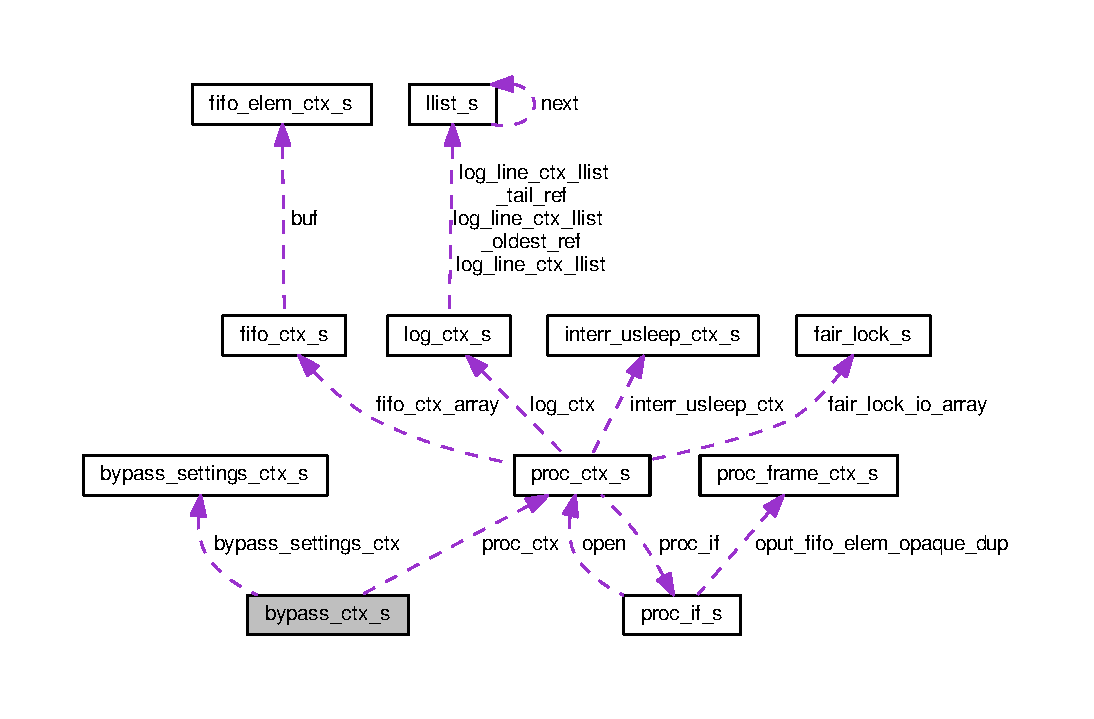
\includegraphics[width=350pt]{structbypass__ctx__s__coll__graph}
\end{center}
\end{figure}
\subsection*{Public Attributes}
\begin{DoxyCompactItemize}
\item 
struct \hyperlink{structproc__ctx__s}{proc\+\_\+ctx\+\_\+s} \hyperlink{structbypass__ctx__s_abc729b752c9d47955160e520a05177fd}{proc\+\_\+ctx}
\item 
volatile struct \hyperlink{structbypass__settings__ctx__s}{bypass\+\_\+settings\+\_\+ctx\+\_\+s} \hyperlink{structbypass__ctx__s_a490fe71a913f9bae1bab3208746d9ab4}{bypass\+\_\+settings\+\_\+ctx}
\end{DoxyCompactItemize}


\subsection{Detailed Description}
Bypass processor context structure. 

Definition at line 52 of file bypass.\+c.



\subsection{Member Data Documentation}
\index{bypass\+\_\+ctx\+\_\+s@{bypass\+\_\+ctx\+\_\+s}!bypass\+\_\+settings\+\_\+ctx@{bypass\+\_\+settings\+\_\+ctx}}
\index{bypass\+\_\+settings\+\_\+ctx@{bypass\+\_\+settings\+\_\+ctx}!bypass\+\_\+ctx\+\_\+s@{bypass\+\_\+ctx\+\_\+s}}
\subsubsection[{\texorpdfstring{bypass\+\_\+settings\+\_\+ctx}{bypass_settings_ctx}}]{\setlength{\rightskip}{0pt plus 5cm}volatile struct {\bf bypass\+\_\+settings\+\_\+ctx\+\_\+s} bypass\+\_\+ctx\+\_\+s\+::bypass\+\_\+settings\+\_\+ctx}\hypertarget{structbypass__ctx__s_a490fe71a913f9bae1bab3208746d9ab4}{}\label{structbypass__ctx__s_a490fe71a913f9bae1bab3208746d9ab4}
Bypass processor settings. 

Definition at line 61 of file bypass.\+c.

\index{bypass\+\_\+ctx\+\_\+s@{bypass\+\_\+ctx\+\_\+s}!proc\+\_\+ctx@{proc\+\_\+ctx}}
\index{proc\+\_\+ctx@{proc\+\_\+ctx}!bypass\+\_\+ctx\+\_\+s@{bypass\+\_\+ctx\+\_\+s}}
\subsubsection[{\texorpdfstring{proc\+\_\+ctx}{proc_ctx}}]{\setlength{\rightskip}{0pt plus 5cm}struct {\bf proc\+\_\+ctx\+\_\+s} bypass\+\_\+ctx\+\_\+s\+::proc\+\_\+ctx}\hypertarget{structbypass__ctx__s_abc729b752c9d47955160e520a05177fd}{}\label{structbypass__ctx__s_abc729b752c9d47955160e520a05177fd}
Generic processor context structure. {\itshape M\+U\+ST} be the first field in order to be able to cast to proc\+\_\+ctx\+\_\+t. 

Definition at line 57 of file bypass.\+c.



The documentation for this struct was generated from the following file\+:\begin{DoxyCompactItemize}
\item 
\hyperlink{bypass_8c}{bypass.\+c}\end{DoxyCompactItemize}

\input{structbypass__proc__ctx__s}
\hypertarget{structbypass__settings__ctx__s}{}\section{bypass\+\_\+settings\+\_\+ctx\+\_\+s Struct Reference}
\label{structbypass__settings__ctx__s}\index{bypass\+\_\+settings\+\_\+ctx\+\_\+s@{bypass\+\_\+settings\+\_\+ctx\+\_\+s}}


\subsection{Detailed Description}
Bypass processor settings context structure. 

Definition at line 45 of file bypass.\+c.



The documentation for this struct was generated from the following file\+:\begin{DoxyCompactItemize}
\item 
\hyperlink{bypass_8c}{bypass.\+c}\end{DoxyCompactItemize}

\hypertarget{structcomm__ctx__s}{}\section{comm\+\_\+ctx\+\_\+s Struct Reference}
\label{structcomm__ctx__s}\index{comm\+\_\+ctx\+\_\+s@{comm\+\_\+ctx\+\_\+s}}


{\ttfamily \#include $<$comm.\+h$>$}



Collaboration diagram for comm\+\_\+ctx\+\_\+s\+:\nopagebreak
\begin{figure}[H]
\begin{center}
\leavevmode
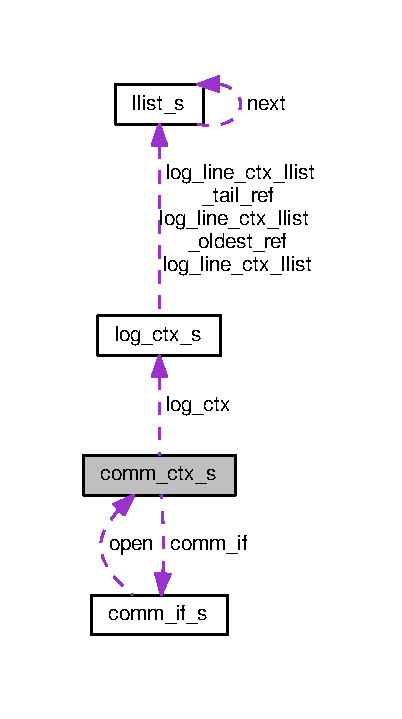
\includegraphics[width=193pt]{structcomm__ctx__s__coll__graph}
\end{center}
\end{figure}
\subsection*{Public Attributes}
\begin{DoxyCompactItemize}
\item 
const \hyperlink{comm_8h_a0d96b9368107e517ea8253837384faf5}{comm\+\_\+if\+\_\+t} $\ast$ \hyperlink{structcomm__ctx__s_ada6c987982f09f27479ce375b5050534}{comm\+\_\+if}
\item 
pthread\+\_\+mutex\+\_\+t \hyperlink{structcomm__ctx__s_a87f4bc5b93d50488325c43f384cb9d61}{api\+\_\+mutex}
\item 
\hyperlink{structlog__ctx__s}{log\+\_\+ctx\+\_\+t} $\ast$ \hyperlink{structcomm__ctx__s_a8ac71b7c3edcbbf9eb98f8668f9fe572}{log\+\_\+ctx}
\item 
\hyperlink{comm_8h_a2604d892f8ab29dfc96bd68e2cc3086f}{comm\+\_\+mode\+\_\+t} \hyperlink{structcomm__ctx__s_a8e47d99809ed21c0d63e53529b3d0596}{comm\+\_\+mode}
\item 
char $\ast$ \hyperlink{structcomm__ctx__s_afa1c9d723a19d1ec55d4ff2e9f8d17e0}{local\+\_\+url}
\item 
char $\ast$ \hyperlink{structcomm__ctx__s_aa5fe745b2131be751f5a0e4528c946d3}{url}
\end{DoxyCompactItemize}


\subsection{Detailed Description}
Communication module instance context structure (\textquotesingle{}handler\textquotesingle{}). 

Definition at line 79 of file comm.\+h.



\subsection{Member Data Documentation}
\index{comm\+\_\+ctx\+\_\+s@{comm\+\_\+ctx\+\_\+s}!api\+\_\+mutex@{api\+\_\+mutex}}
\index{api\+\_\+mutex@{api\+\_\+mutex}!comm\+\_\+ctx\+\_\+s@{comm\+\_\+ctx\+\_\+s}}
\subsubsection[{\texorpdfstring{api\+\_\+mutex}{api_mutex}}]{\setlength{\rightskip}{0pt plus 5cm}pthread\+\_\+mutex\+\_\+t comm\+\_\+ctx\+\_\+s\+::api\+\_\+mutex}\hypertarget{structcomm__ctx__s_a87f4bc5b93d50488325c43f384cb9d61}{}\label{structcomm__ctx__s_a87f4bc5b93d50488325c43f384cb9d61}
Module instance A\+PI mutual exclusion lock. 

Definition at line 87 of file comm.\+h.

\index{comm\+\_\+ctx\+\_\+s@{comm\+\_\+ctx\+\_\+s}!comm\+\_\+if@{comm\+\_\+if}}
\index{comm\+\_\+if@{comm\+\_\+if}!comm\+\_\+ctx\+\_\+s@{comm\+\_\+ctx\+\_\+s}}
\subsubsection[{\texorpdfstring{comm\+\_\+if}{comm_if}}]{\setlength{\rightskip}{0pt plus 5cm}const {\bf comm\+\_\+if\+\_\+t}$\ast$ comm\+\_\+ctx\+\_\+s\+::comm\+\_\+if}\hypertarget{structcomm__ctx__s_ada6c987982f09f27479ce375b5050534}{}\label{structcomm__ctx__s_ada6c987982f09f27479ce375b5050534}
Communication interface structure prototype. 

Definition at line 83 of file comm.\+h.

\index{comm\+\_\+ctx\+\_\+s@{comm\+\_\+ctx\+\_\+s}!comm\+\_\+mode@{comm\+\_\+mode}}
\index{comm\+\_\+mode@{comm\+\_\+mode}!comm\+\_\+ctx\+\_\+s@{comm\+\_\+ctx\+\_\+s}}
\subsubsection[{\texorpdfstring{comm\+\_\+mode}{comm_mode}}]{\setlength{\rightskip}{0pt plus 5cm}{\bf comm\+\_\+mode\+\_\+t} comm\+\_\+ctx\+\_\+s\+::comm\+\_\+mode}\hypertarget{structcomm__ctx__s_a8e47d99809ed21c0d63e53529b3d0596}{}\label{structcomm__ctx__s_a8e47d99809ed21c0d63e53529b3d0596}
Module instance mode. 

Definition at line 95 of file comm.\+h.

\index{comm\+\_\+ctx\+\_\+s@{comm\+\_\+ctx\+\_\+s}!local\+\_\+url@{local\+\_\+url}}
\index{local\+\_\+url@{local\+\_\+url}!comm\+\_\+ctx\+\_\+s@{comm\+\_\+ctx\+\_\+s}}
\subsubsection[{\texorpdfstring{local\+\_\+url}{local_url}}]{\setlength{\rightskip}{0pt plus 5cm}char$\ast$ comm\+\_\+ctx\+\_\+s\+::local\+\_\+url}\hypertarget{structcomm__ctx__s_afa1c9d723a19d1ec55d4ff2e9f8d17e0}{}\label{structcomm__ctx__s_afa1c9d723a19d1ec55d4ff2e9f8d17e0}
Local U\+RL. 

Definition at line 99 of file comm.\+h.

\index{comm\+\_\+ctx\+\_\+s@{comm\+\_\+ctx\+\_\+s}!log\+\_\+ctx@{log\+\_\+ctx}}
\index{log\+\_\+ctx@{log\+\_\+ctx}!comm\+\_\+ctx\+\_\+s@{comm\+\_\+ctx\+\_\+s}}
\subsubsection[{\texorpdfstring{log\+\_\+ctx}{log_ctx}}]{\setlength{\rightskip}{0pt plus 5cm}{\bf log\+\_\+ctx\+\_\+t}$\ast$ comm\+\_\+ctx\+\_\+s\+::log\+\_\+ctx}\hypertarget{structcomm__ctx__s_a8ac71b7c3edcbbf9eb98f8668f9fe572}{}\label{structcomm__ctx__s_a8ac71b7c3edcbbf9eb98f8668f9fe572}
External L\+OG module context structure instance. 

Definition at line 91 of file comm.\+h.

\index{comm\+\_\+ctx\+\_\+s@{comm\+\_\+ctx\+\_\+s}!url@{url}}
\index{url@{url}!comm\+\_\+ctx\+\_\+s@{comm\+\_\+ctx\+\_\+s}}
\subsubsection[{\texorpdfstring{url}{url}}]{\setlength{\rightskip}{0pt plus 5cm}char$\ast$ comm\+\_\+ctx\+\_\+s\+::url}\hypertarget{structcomm__ctx__s_aa5fe745b2131be751f5a0e4528c946d3}{}\label{structcomm__ctx__s_aa5fe745b2131be751f5a0e4528c946d3}
Input/output U\+RL. 

Definition at line 103 of file comm.\+h.



The documentation for this struct was generated from the following file\+:\begin{DoxyCompactItemize}
\item 
\hyperlink{comm_8h}{comm.\+h}\end{DoxyCompactItemize}

\hypertarget{structcomm__if__s}{}\section{comm\+\_\+if\+\_\+s Struct Reference}
\label{structcomm__if__s}\index{comm\+\_\+if\+\_\+s@{comm\+\_\+if\+\_\+s}}


{\ttfamily \#include $<$comm.\+h$>$}



Collaboration diagram for comm\+\_\+if\+\_\+s\+:\nopagebreak
\begin{figure}[H]
\begin{center}
\leavevmode
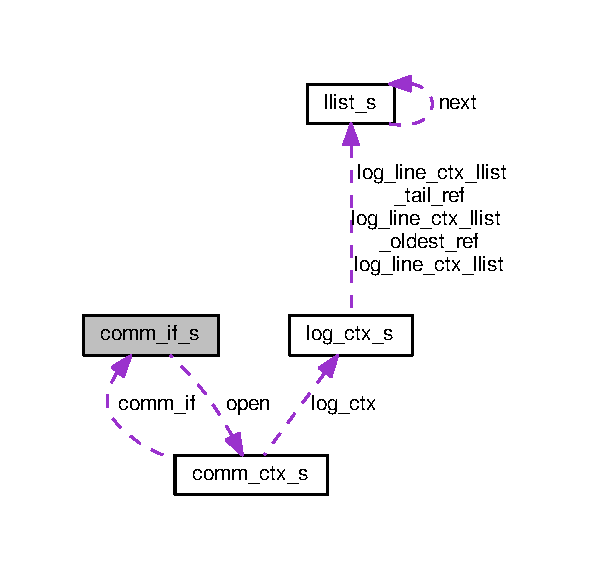
\includegraphics[width=285pt]{structcomm__if__s__coll__graph}
\end{center}
\end{figure}
\subsection*{Public Attributes}
\begin{DoxyCompactItemize}
\item 
char $\ast$ {\bfseries scheme}\hypertarget{structcomm__if__s_a46d130ec366e00c748848f1666bd168e}{}\label{structcomm__if__s_a46d130ec366e00c748848f1666bd168e}

\item 
\hyperlink{comm_8h_aacc0873718a86d8ef4658bad2500d091}{comm\+\_\+ctx\+\_\+t} $\ast$($\ast$ {\bfseries open} )(const char $\ast$url, const char $\ast$local\+\_\+url, \hyperlink{comm_8h_a2604d892f8ab29dfc96bd68e2cc3086f}{comm\+\_\+mode\+\_\+t} comm\+\_\+mode, \hyperlink{structlog__ctx__s}{log\+\_\+ctx\+\_\+t} $\ast$log\+\_\+ctx, va\+\_\+list arg)\hypertarget{structcomm__if__s_ac8bba953c88fa636aeff682e116fa9d1}{}\label{structcomm__if__s_ac8bba953c88fa636aeff682e116fa9d1}

\item 
void($\ast$ {\bfseries close} )(\hyperlink{comm_8h_aacc0873718a86d8ef4658bad2500d091}{comm\+\_\+ctx\+\_\+t} $\ast$$\ast$ref\+\_\+comm\+\_\+ctx)\hypertarget{structcomm__if__s_a077eba49a8a8189a250868920e925956}{}\label{structcomm__if__s_a077eba49a8a8189a250868920e925956}

\item 
int($\ast$ {\bfseries send} )(\hyperlink{comm_8h_aacc0873718a86d8ef4658bad2500d091}{comm\+\_\+ctx\+\_\+t} $\ast$comm\+\_\+ctx, const void $\ast$buf, size\+\_\+t count, struct timeval $\ast$timeout)\hypertarget{structcomm__if__s_aea8ef75cc832cd88f0a8f8fcccc00f48}{}\label{structcomm__if__s_aea8ef75cc832cd88f0a8f8fcccc00f48}

\item 
int($\ast$ {\bfseries recv} )(\hyperlink{comm_8h_aacc0873718a86d8ef4658bad2500d091}{comm\+\_\+ctx\+\_\+t} $\ast$comm\+\_\+ctx, void $\ast$$\ast$ref\+\_\+buf, size\+\_\+t $\ast$ref\+\_\+count, char $\ast$$\ast$ref\+\_\+from, struct timeval $\ast$timeout)\hypertarget{structcomm__if__s_a28e7de5768bc096208c18aaf41c1e2a1}{}\label{structcomm__if__s_a28e7de5768bc096208c18aaf41c1e2a1}

\item 
int($\ast$ {\bfseries unblock} )(\hyperlink{comm_8h_aacc0873718a86d8ef4658bad2500d091}{comm\+\_\+ctx\+\_\+t} $\ast$comm\+\_\+ctx)\hypertarget{structcomm__if__s_ad5d4d1d4399aef10770a07372455ca80}{}\label{structcomm__if__s_ad5d4d1d4399aef10770a07372455ca80}

\end{DoxyCompactItemize}


\subsection{Detailed Description}
Communication protocol interface structure prototype. Each specific communication module implementation will define a static and unambiguous interface of this type. 

Definition at line 64 of file comm.\+h.



The documentation for this struct was generated from the following file\+:\begin{DoxyCompactItemize}
\item 
\hyperlink{comm_8h}{comm.\+h}\end{DoxyCompactItemize}

\hypertarget{structcomm__module__ctx__s}{}\section{comm\+\_\+module\+\_\+ctx\+\_\+s Struct Reference}
\label{structcomm__module__ctx__s}\index{comm\+\_\+module\+\_\+ctx\+\_\+s@{comm\+\_\+module\+\_\+ctx\+\_\+s}}


Collaboration diagram for comm\+\_\+module\+\_\+ctx\+\_\+s\+:\nopagebreak
\begin{figure}[H]
\begin{center}
\leavevmode
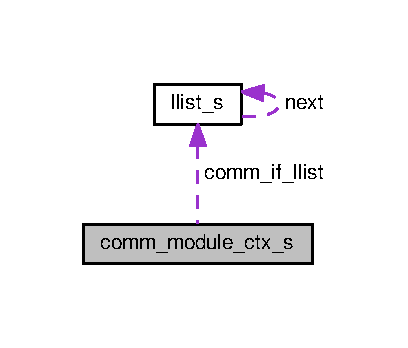
\includegraphics[width=196pt]{structcomm__module__ctx__s__coll__graph}
\end{center}
\end{figure}
\subsection*{Public Attributes}
\begin{DoxyCompactItemize}
\item 
pthread\+\_\+mutex\+\_\+t \hyperlink{structcomm__module__ctx__s_a065cf60f09cc13971556a494dc35425f}{module\+\_\+api\+\_\+mutex}
\item 
\hyperlink{llist_8h_a90862badf6f9cc4e3d6348b7d60ce4f0}{llist\+\_\+t} $\ast$ \hyperlink{structcomm__module__ctx__s_aca7d8c9e08de7feabe5818c35abd2244}{comm\+\_\+if\+\_\+llist}
\end{DoxyCompactItemize}


\subsection{Detailed Description}
Module\textquotesingle{}s context structure. This structure is statically defined in the program. 

Definition at line 62 of file comm.\+c.



\subsection{Member Data Documentation}
\index{comm\+\_\+module\+\_\+ctx\+\_\+s@{comm\+\_\+module\+\_\+ctx\+\_\+s}!comm\+\_\+if\+\_\+llist@{comm\+\_\+if\+\_\+llist}}
\index{comm\+\_\+if\+\_\+llist@{comm\+\_\+if\+\_\+llist}!comm\+\_\+module\+\_\+ctx\+\_\+s@{comm\+\_\+module\+\_\+ctx\+\_\+s}}
\subsubsection[{\texorpdfstring{comm\+\_\+if\+\_\+llist}{comm_if_llist}}]{\setlength{\rightskip}{0pt plus 5cm}{\bf llist\+\_\+t}$\ast$ comm\+\_\+module\+\_\+ctx\+\_\+s\+::comm\+\_\+if\+\_\+llist}\hypertarget{structcomm__module__ctx__s_aca7d8c9e08de7feabe5818c35abd2244}{}\label{structcomm__module__ctx__s_aca7d8c9e08de7feabe5818c35abd2244}
List of supported/registered communication protocols. Each registered protocol will have a static interface (IF) entry in this linked list. \begin{DoxySeeAlso}{See also}
\hyperlink{comm_8h_a0d96b9368107e517ea8253837384faf5}{comm\+\_\+if\+\_\+t} 
\end{DoxySeeAlso}


Definition at line 77 of file comm.\+c.

\index{comm\+\_\+module\+\_\+ctx\+\_\+s@{comm\+\_\+module\+\_\+ctx\+\_\+s}!module\+\_\+api\+\_\+mutex@{module\+\_\+api\+\_\+mutex}}
\index{module\+\_\+api\+\_\+mutex@{module\+\_\+api\+\_\+mutex}!comm\+\_\+module\+\_\+ctx\+\_\+s@{comm\+\_\+module\+\_\+ctx\+\_\+s}}
\subsubsection[{\texorpdfstring{module\+\_\+api\+\_\+mutex}{module_api_mutex}}]{\setlength{\rightskip}{0pt plus 5cm}pthread\+\_\+mutex\+\_\+t comm\+\_\+module\+\_\+ctx\+\_\+s\+::module\+\_\+api\+\_\+mutex}\hypertarget{structcomm__module__ctx__s_a065cf60f09cc13971556a494dc35425f}{}\label{structcomm__module__ctx__s_a065cf60f09cc13971556a494dc35425f}
Module\textquotesingle{}s A\+PI mutual exclusion lock. This lock is used to provide a critical section for external applications to be able to operate concurrently and asynchronously on this module. A\+PI options are available through the function \hyperlink{comm_8c_a21edd1aa9b38d7eadecb70b5f963f437}{comm\+\_\+module\+\_\+opt()}. 

Definition at line 70 of file comm.\+c.



The documentation for this struct was generated from the following file\+:\begin{DoxyCompactItemize}
\item 
\hyperlink{comm_8c}{comm.\+c}\end{DoxyCompactItemize}

\hypertarget{structcomm__udp__ctx__s}{}\section{comm\+\_\+udp\+\_\+ctx\+\_\+s Struct Reference}
\label{structcomm__udp__ctx__s}\index{comm\+\_\+udp\+\_\+ctx\+\_\+s@{comm\+\_\+udp\+\_\+ctx\+\_\+s}}


Collaboration diagram for comm\+\_\+udp\+\_\+ctx\+\_\+s\+:\nopagebreak
\begin{figure}[H]
\begin{center}
\leavevmode
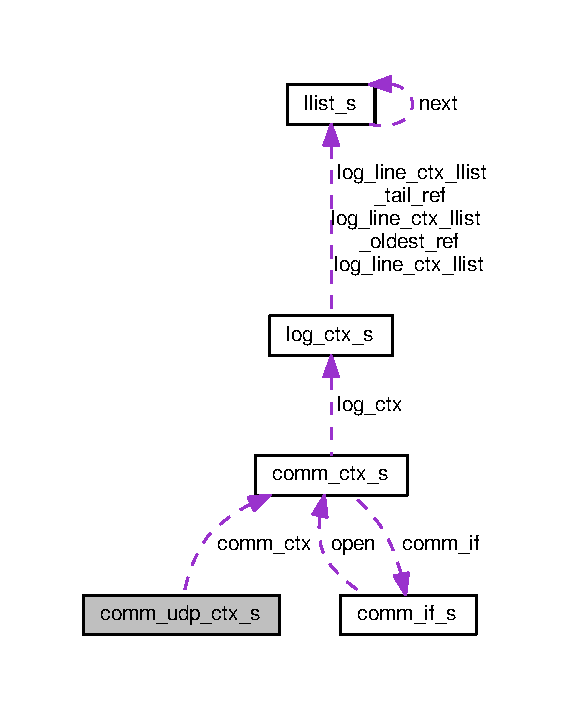
\includegraphics[width=275pt]{structcomm__udp__ctx__s__coll__graph}
\end{center}
\end{figure}
\subsection*{Public Attributes}
\begin{DoxyCompactItemize}
\item 
struct \hyperlink{structcomm__ctx__s}{comm\+\_\+ctx\+\_\+s} \hyperlink{structcomm__udp__ctx__s_a3732c33a70c43d9f270ab912cc23d94b}{comm\+\_\+ctx}
\item 
int \hyperlink{structcomm__udp__ctx__s_a65be1c0c98d73e09419c3507a4c4535b}{fd}
\item 
volatile int \hyperlink{structcomm__udp__ctx__s_a3478e148fc2c7e2a11d0ecf1f064ad27}{flag\+\_\+exit}
\item 
int \hyperlink{structcomm__udp__ctx__s_af98857f20d566dca629dbe52a7f8e57c}{pipe\+\_\+exit\+\_\+signal} \mbox{[}2\mbox{]}
\end{DoxyCompactItemize}


\subsection{Detailed Description}
Module instance context structure 

Definition at line 65 of file comm\+\_\+udp.\+c.



\subsection{Member Data Documentation}
\index{comm\+\_\+udp\+\_\+ctx\+\_\+s@{comm\+\_\+udp\+\_\+ctx\+\_\+s}!comm\+\_\+ctx@{comm\+\_\+ctx}}
\index{comm\+\_\+ctx@{comm\+\_\+ctx}!comm\+\_\+udp\+\_\+ctx\+\_\+s@{comm\+\_\+udp\+\_\+ctx\+\_\+s}}
\subsubsection[{\texorpdfstring{comm\+\_\+ctx}{comm_ctx}}]{\setlength{\rightskip}{0pt plus 5cm}struct {\bf comm\+\_\+ctx\+\_\+s} comm\+\_\+udp\+\_\+ctx\+\_\+s\+::comm\+\_\+ctx}\hypertarget{structcomm__udp__ctx__s_a3732c33a70c43d9f270ab912cc23d94b}{}\label{structcomm__udp__ctx__s_a3732c33a70c43d9f270ab912cc23d94b}
Generic communication interface structure. {\itshape M\+U\+ST} be the first field in order to be able to cast to both comm\+\_\+udp\+\_\+ctx\+\_\+t or comm\+\_\+udp\+\_\+ctx\+\_\+t. 

Definition at line 71 of file comm\+\_\+udp.\+c.

\index{comm\+\_\+udp\+\_\+ctx\+\_\+s@{comm\+\_\+udp\+\_\+ctx\+\_\+s}!fd@{fd}}
\index{fd@{fd}!comm\+\_\+udp\+\_\+ctx\+\_\+s@{comm\+\_\+udp\+\_\+ctx\+\_\+s}}
\subsubsection[{\texorpdfstring{fd}{fd}}]{\setlength{\rightskip}{0pt plus 5cm}int comm\+\_\+udp\+\_\+ctx\+\_\+s\+::fd}\hypertarget{structcomm__udp__ctx__s_a65be1c0c98d73e09419c3507a4c4535b}{}\label{structcomm__udp__ctx__s_a65be1c0c98d73e09419c3507a4c4535b}
Socket file descriptor 

Definition at line 75 of file comm\+\_\+udp.\+c.

\index{comm\+\_\+udp\+\_\+ctx\+\_\+s@{comm\+\_\+udp\+\_\+ctx\+\_\+s}!flag\+\_\+exit@{flag\+\_\+exit}}
\index{flag\+\_\+exit@{flag\+\_\+exit}!comm\+\_\+udp\+\_\+ctx\+\_\+s@{comm\+\_\+udp\+\_\+ctx\+\_\+s}}
\subsubsection[{\texorpdfstring{flag\+\_\+exit}{flag_exit}}]{\setlength{\rightskip}{0pt plus 5cm}volatile int comm\+\_\+udp\+\_\+ctx\+\_\+s\+::flag\+\_\+exit}\hypertarget{structcomm__udp__ctx__s_a3478e148fc2c7e2a11d0ecf1f064ad27}{}\label{structcomm__udp__ctx__s_a3478e148fc2c7e2a11d0ecf1f064ad27}
Exit flag\+: if set to non-\/zero value, module should finish/unblock transactions as fast as possible 

Definition at line 80 of file comm\+\_\+udp.\+c.

\index{comm\+\_\+udp\+\_\+ctx\+\_\+s@{comm\+\_\+udp\+\_\+ctx\+\_\+s}!pipe\+\_\+exit\+\_\+signal@{pipe\+\_\+exit\+\_\+signal}}
\index{pipe\+\_\+exit\+\_\+signal@{pipe\+\_\+exit\+\_\+signal}!comm\+\_\+udp\+\_\+ctx\+\_\+s@{comm\+\_\+udp\+\_\+ctx\+\_\+s}}
\subsubsection[{\texorpdfstring{pipe\+\_\+exit\+\_\+signal}{pipe_exit_signal}}]{\setlength{\rightskip}{0pt plus 5cm}int comm\+\_\+udp\+\_\+ctx\+\_\+s\+::pipe\+\_\+exit\+\_\+signal\mbox{[}2\mbox{]}}\hypertarget{structcomm__udp__ctx__s_af98857f20d566dca629dbe52a7f8e57c}{}\label{structcomm__udp__ctx__s_af98857f20d566dca629dbe52a7f8e57c}
This pipe is used exclusively for the purpose of abruptly closing U\+D\+P-\/com module; the pipe is used to wake-\/up any \textquotesingle{}select()\textquotesingle{} waiting for incoming data. 

Definition at line 86 of file comm\+\_\+udp.\+c.



The documentation for this struct was generated from the following file\+:\begin{DoxyCompactItemize}
\item 
\hyperlink{comm__udp_8c}{comm\+\_\+udp.\+c}\end{DoxyCompactItemize}

\hypertarget{classDummySink}{}\section{Dummy\+Sink Class Reference}
\label{classDummySink}\index{Dummy\+Sink@{Dummy\+Sink}}


Inheritance diagram for Dummy\+Sink\+:\nopagebreak
\begin{figure}[H]
\begin{center}
\leavevmode
\includegraphics[width=151pt]{classDummySink__inherit__graph}
\end{center}
\end{figure}


Collaboration diagram for Dummy\+Sink\+:\nopagebreak
\begin{figure}[H]
\begin{center}
\leavevmode
\includegraphics[width=151pt]{classDummySink__coll__graph}
\end{center}
\end{figure}
\subsection*{Static Public Member Functions}
\begin{DoxyCompactItemize}
\item 
static \hyperlink{classDummySink}{Dummy\+Sink} $\ast$ \hyperlink{classDummySink_af1d373302d3f27791ac565136321765b}{create\+New} (Usage\+Environment \&env, Media\+Subsession \&subsession, \hyperlink{fifo_8c_acf3f21e64cbabccd8420c306740820c1}{fifo\+\_\+ctx\+\_\+t} $\ast$fifo\+\_\+ctx, char const $\ast$stream\+Id=N\+U\+LL, \hyperlink{structlog__ctx__s}{log\+\_\+ctx\+\_\+t} $\ast$log\+\_\+ctx=N\+U\+LL)
\end{DoxyCompactItemize}


\subsection{Detailed Description}
Define a data sink (a subclass of \char`\"{}\+Media\+Sink\char`\"{}) to receive the data for each sub-\/session (i.\+e., each audio or video \textquotesingle{}sub-\/stream\textquotesingle{}). 

Definition at line 504 of file live555\+\_\+rtsp.\+cpp.



\subsection{Member Function Documentation}
\index{Dummy\+Sink@{Dummy\+Sink}!create\+New@{create\+New}}
\index{create\+New@{create\+New}!Dummy\+Sink@{Dummy\+Sink}}
\subsubsection[{\texorpdfstring{create\+New(\+Usage\+Environment \&env, Media\+Subsession \&subsession, fifo\+\_\+ctx\+\_\+t $\ast$fifo\+\_\+ctx, char const $\ast$stream\+Id=\+N\+U\+L\+L, log\+\_\+ctx\+\_\+t $\ast$log\+\_\+ctx=\+N\+U\+L\+L)}{createNew(UsageEnvironment &env, MediaSubsession &subsession, fifo_ctx_t *fifo_ctx, char const *streamId=NULL, log_ctx_t *log_ctx=NULL)}}]{\setlength{\rightskip}{0pt plus 5cm}{\bf Dummy\+Sink} $\ast$ Dummy\+Sink\+::create\+New (
\begin{DoxyParamCaption}
\item[{Usage\+Environment \&}]{env, }
\item[{Media\+Subsession \&}]{subsession, }
\item[{{\bf fifo\+\_\+ctx\+\_\+t} $\ast$}]{fifo\+\_\+ctx, }
\item[{char const $\ast$}]{stream\+Id = {\ttfamily NULL}, }
\item[{{\bf log\+\_\+ctx\+\_\+t} $\ast$}]{log\+\_\+ctx = {\ttfamily NULL}}
\end{DoxyParamCaption}
)\hspace{0.3cm}{\ttfamily [static]}}\hypertarget{classDummySink_af1d373302d3f27791ac565136321765b}{}\label{classDummySink_af1d373302d3f27791ac565136321765b}

\begin{DoxyParams}{Parameters}
{\em env} & \\
\hline
{\em subsession} & Identifies the kind of data that\textquotesingle{}s being received \\
\hline
{\em stream\+Id} & Identifies the stream itself (optional) \\
\hline
\end{DoxyParams}


Definition at line 2999 of file live555\+\_\+rtsp.\+cpp.



The documentation for this class was generated from the following file\+:\begin{DoxyCompactItemize}
\item 
\hyperlink{live555__rtsp_8cpp}{live555\+\_\+rtsp.\+cpp}\end{DoxyCompactItemize}

\input{structev__user__data__s}
\input{structfair__lock__s}
\input{structffmpeg__audio__dec__ctx__s}
\input{structffmpeg__audio__enc__ctx__s}
\input{structffmpeg__m2v__dec__ctx__s}
\input{structffmpeg__m2v__dec__settings__ctx__s}
\input{structffmpeg__m2v__enc__ctx__s}
\input{structffmpeg__m2v__enc__settings__ctx__s}
\input{structffmpeg__mlhe__dec__ctx__s}
\input{structffmpeg__mlhe__dec__settings__ctx__s}
\input{structffmpeg__mlhe__enc__ctx__s}
\input{structffmpeg__mlhe__enc__settings__ctx__s}
\input{structffmpeg__mp3__dec__ctx__s}
\input{structffmpeg__mp3__dec__settings__ctx__s}
\input{structffmpeg__mp3__enc__ctx__s}
\input{structffmpeg__mp3__enc__settings__ctx__s}
\input{structffmpeg__video__dec__ctx__s}
\input{structffmpeg__video__enc__ctx__s}
\input{structffmpeg__x264__dec__ctx__s}
\input{structffmpeg__x264__dec__settings__ctx__s}
\input{structffmpeg__x264__enc__ctx__s}
\input{structffmpeg__x264__enc__settings__ctx__s}
\hypertarget{structfifo__ctx__s}{}\section{fifo\+\_\+ctx\+\_\+s Struct Reference}
\label{structfifo__ctx__s}\index{fifo\+\_\+ctx\+\_\+s@{fifo\+\_\+ctx\+\_\+s}}


Collaboration diagram for fifo\+\_\+ctx\+\_\+s\+:\nopagebreak
\begin{figure}[H]
\begin{center}
\leavevmode
\includegraphics[width=166pt]{structfifo__ctx__s__coll__graph}
\end{center}
\end{figure}
\subsection*{Public Attributes}
\begin{DoxyCompactItemize}
\item 
volatile uint32\+\_\+t \hyperlink{structfifo__ctx__s_a6c86ce21bbd7a84d164d9c5ecf72ac3a}{flags}
\item 
volatile int \hyperlink{structfifo__ctx__s_a4856c98e4576bd328ff3ee4063b1421a}{flag\+\_\+exit}
\item 
char {\bfseries fifo\+\_\+file\+\_\+name} \mbox{[}\hyperlink{fifo_8c_a42708bf618db9ea973b091a2d5bdfa9e}{F\+I\+F\+O\+\_\+\+F\+I\+L\+E\+\_\+\+N\+A\+M\+E\+\_\+\+M\+A\+X\+\_\+\+S\+I\+ZE}\mbox{]}\hypertarget{structfifo__ctx__s_ad94e9742a0fe4eff3cd6bbc9501ca872}{}\label{structfifo__ctx__s_ad94e9742a0fe4eff3cd6bbc9501ca872}

\item 
fifo\+\_\+elem\+\_\+ctx\+\_\+dup\+\_\+fxn\+\_\+t $\ast$ \hyperlink{structfifo__ctx__s_a29fe5cab2bded769f7aff0050877aa65}{elem\+\_\+ctx\+\_\+dup}
\item 
fifo\+\_\+elem\+\_\+ctx\+\_\+release\+\_\+fxn\+\_\+t $\ast$ \hyperlink{structfifo__ctx__s_a5d110b8cfb21fe7f732ba5efc0013d59}{elem\+\_\+ctx\+\_\+release}
\item 
pthread\+\_\+mutex\+\_\+t \hyperlink{structfifo__ctx__s_a27be272ae3fa045dfb5e64778a484725}{api\+\_\+mutex}
\item 
int {\bfseries flag\+\_\+api\+\_\+mutex\+\_\+initialized}\hypertarget{structfifo__ctx__s_a4c003f60d37a471dc9f5bf517df52608}{}\label{structfifo__ctx__s_a4c003f60d37a471dc9f5bf517df52608}

\item 
pthread\+\_\+cond\+\_\+t \hyperlink{structfifo__ctx__s_a3f9e6f9e1505a9f7e1756c212602a9df}{buf\+\_\+put\+\_\+signal}
\item 
int {\bfseries flag\+\_\+buf\+\_\+put\+\_\+signal\+\_\+initialized}\hypertarget{structfifo__ctx__s_adb6724f4e6b09980696d3e71440b8804}{}\label{structfifo__ctx__s_adb6724f4e6b09980696d3e71440b8804}

\item 
pthread\+\_\+cond\+\_\+t \hyperlink{structfifo__ctx__s_af13501e5f83d5d1561bf76577c490f23}{buf\+\_\+get\+\_\+signal}
\item 
int {\bfseries flag\+\_\+buf\+\_\+get\+\_\+signal\+\_\+initialized}\hypertarget{structfifo__ctx__s_af1ee1332ce2af0a6bd6e77e7e99c4ca1}{}\label{structfifo__ctx__s_af1ee1332ce2af0a6bd6e77e7e99c4ca1}

\item 
volatile ssize\+\_\+t \hyperlink{structfifo__ctx__s_a566e90d020d2b7a45b6a8879c63106c2}{slots\+\_\+used\+\_\+cnt}
\item 
volatile ssize\+\_\+t \hyperlink{structfifo__ctx__s_a9661ff316afd08e4eb0919cd02e355ce}{buf\+\_\+level}
\item 
volatile int \hyperlink{structfifo__ctx__s_aa5c17b3a497d655710243cb2c14ef1bf}{input\+\_\+idx}
\item 
volatile int \hyperlink{structfifo__ctx__s_a28fca425f183a3add55c94dcdc5c04e0}{output\+\_\+idx}
\item 
size\+\_\+t \hyperlink{structfifo__ctx__s_a9e7f97c83e08c4dff68c1f4dedb25537}{buf\+\_\+slots\+\_\+max}
\item 
size\+\_\+t \hyperlink{structfifo__ctx__s_ab67621fb3c666a07ada8a20d03e3c26c}{chunk\+\_\+size\+\_\+max}
\item 
\hyperlink{fifo_8c_a3236a0200db719fdeb6d875a415ca7c9}{fifo\+\_\+elem\+\_\+ctx\+\_\+t} \hyperlink{structfifo__ctx__s_aaff82bce9d68fd7f61378270841b4969}{buf} \mbox{[}$\,$\mbox{]}
\end{DoxyCompactItemize}


\subsection{Detailed Description}
F\+I\+FO context structure. 

Definition at line 87 of file fifo.\+c.



\subsection{Member Data Documentation}
\index{fifo\+\_\+ctx\+\_\+s@{fifo\+\_\+ctx\+\_\+s}!api\+\_\+mutex@{api\+\_\+mutex}}
\index{api\+\_\+mutex@{api\+\_\+mutex}!fifo\+\_\+ctx\+\_\+s@{fifo\+\_\+ctx\+\_\+s}}
\subsubsection[{\texorpdfstring{api\+\_\+mutex}{api_mutex}}]{\setlength{\rightskip}{0pt plus 5cm}pthread\+\_\+mutex\+\_\+t fifo\+\_\+ctx\+\_\+s\+::api\+\_\+mutex}\hypertarget{structfifo__ctx__s_a27be272ae3fa045dfb5e64778a484725}{}\label{structfifo__ctx__s_a27be272ae3fa045dfb5e64778a484725}
Module A\+PI mutex. 

Definition at line 119 of file fifo.\+c.

\index{fifo\+\_\+ctx\+\_\+s@{fifo\+\_\+ctx\+\_\+s}!buf@{buf}}
\index{buf@{buf}!fifo\+\_\+ctx\+\_\+s@{fifo\+\_\+ctx\+\_\+s}}
\subsubsection[{\texorpdfstring{buf}{buf}}]{\setlength{\rightskip}{0pt plus 5cm}{\bf fifo\+\_\+elem\+\_\+ctx\+\_\+t} fifo\+\_\+ctx\+\_\+s\+::buf\mbox{[}$\,$\mbox{]}}\hypertarget{structfifo__ctx__s_aaff82bce9d68fd7f61378270841b4969}{}\label{structfifo__ctx__s_aaff82bce9d68fd7f61378270841b4969}
This is a circular buffer of pointers to chunks of data. Instead of managing a single pool of data, the buffer stores pointers to a fixed number of chunk objects, each one holding the reference and the size of each chunk. 

Definition at line 172 of file fifo.\+c.

\index{fifo\+\_\+ctx\+\_\+s@{fifo\+\_\+ctx\+\_\+s}!buf\+\_\+get\+\_\+signal@{buf\+\_\+get\+\_\+signal}}
\index{buf\+\_\+get\+\_\+signal@{buf\+\_\+get\+\_\+signal}!fifo\+\_\+ctx\+\_\+s@{fifo\+\_\+ctx\+\_\+s}}
\subsubsection[{\texorpdfstring{buf\+\_\+get\+\_\+signal}{buf_get_signal}}]{\setlength{\rightskip}{0pt plus 5cm}pthread\+\_\+cond\+\_\+t fifo\+\_\+ctx\+\_\+s\+::buf\+\_\+get\+\_\+signal}\hypertarget{structfifo__ctx__s_af13501e5f83d5d1561bf76577c490f23}{}\label{structfifo__ctx__s_af13501e5f83d5d1561bf76577c490f23}
Signals each time a new chunk is consumed from the F\+I\+FO buffer. 

Definition at line 129 of file fifo.\+c.

\index{fifo\+\_\+ctx\+\_\+s@{fifo\+\_\+ctx\+\_\+s}!buf\+\_\+level@{buf\+\_\+level}}
\index{buf\+\_\+level@{buf\+\_\+level}!fifo\+\_\+ctx\+\_\+s@{fifo\+\_\+ctx\+\_\+s}}
\subsubsection[{\texorpdfstring{buf\+\_\+level}{buf_level}}]{\setlength{\rightskip}{0pt plus 5cm}volatile ssize\+\_\+t fifo\+\_\+ctx\+\_\+s\+::buf\+\_\+level}\hypertarget{structfifo__ctx__s_a9661ff316afd08e4eb0919cd02e355ce}{}\label{structfifo__ctx__s_a9661ff316afd08e4eb0919cd02e355ce}
Summation of all the size values of the chunk-\/buffers that compose the input buffer. Namely, is the overall input buffer level. 

Definition at line 139 of file fifo.\+c.

\index{fifo\+\_\+ctx\+\_\+s@{fifo\+\_\+ctx\+\_\+s}!buf\+\_\+put\+\_\+signal@{buf\+\_\+put\+\_\+signal}}
\index{buf\+\_\+put\+\_\+signal@{buf\+\_\+put\+\_\+signal}!fifo\+\_\+ctx\+\_\+s@{fifo\+\_\+ctx\+\_\+s}}
\subsubsection[{\texorpdfstring{buf\+\_\+put\+\_\+signal}{buf_put_signal}}]{\setlength{\rightskip}{0pt plus 5cm}pthread\+\_\+cond\+\_\+t fifo\+\_\+ctx\+\_\+s\+::buf\+\_\+put\+\_\+signal}\hypertarget{structfifo__ctx__s_a3f9e6f9e1505a9f7e1756c212602a9df}{}\label{structfifo__ctx__s_a3f9e6f9e1505a9f7e1756c212602a9df}
Signals each time a new chunk enters the F\+I\+FO buffer. 

Definition at line 124 of file fifo.\+c.

\index{fifo\+\_\+ctx\+\_\+s@{fifo\+\_\+ctx\+\_\+s}!buf\+\_\+slots\+\_\+max@{buf\+\_\+slots\+\_\+max}}
\index{buf\+\_\+slots\+\_\+max@{buf\+\_\+slots\+\_\+max}!fifo\+\_\+ctx\+\_\+s@{fifo\+\_\+ctx\+\_\+s}}
\subsubsection[{\texorpdfstring{buf\+\_\+slots\+\_\+max}{buf_slots_max}}]{\setlength{\rightskip}{0pt plus 5cm}size\+\_\+t fifo\+\_\+ctx\+\_\+s\+::buf\+\_\+slots\+\_\+max}\hypertarget{structfifo__ctx__s_a9e7f97c83e08c4dff68c1f4dedb25537}{}\label{structfifo__ctx__s_a9e7f97c83e08c4dff68c1f4dedb25537}
Maximum number of element-\/slots (namely, maximum number of possible chunks) of the F\+I\+FO buffer. 

Definition at line 157 of file fifo.\+c.

\index{fifo\+\_\+ctx\+\_\+s@{fifo\+\_\+ctx\+\_\+s}!chunk\+\_\+size\+\_\+max@{chunk\+\_\+size\+\_\+max}}
\index{chunk\+\_\+size\+\_\+max@{chunk\+\_\+size\+\_\+max}!fifo\+\_\+ctx\+\_\+s@{fifo\+\_\+ctx\+\_\+s}}
\subsubsection[{\texorpdfstring{chunk\+\_\+size\+\_\+max}{chunk_size_max}}]{\setlength{\rightskip}{0pt plus 5cm}size\+\_\+t fifo\+\_\+ctx\+\_\+s\+::chunk\+\_\+size\+\_\+max}\hypertarget{structfifo__ctx__s_ab67621fb3c666a07ada8a20d03e3c26c}{}\label{structfifo__ctx__s_ab67621fb3c666a07ada8a20d03e3c26c}
Maximum permitted size of chunks \mbox{[}bytes\mbox{]}. In the case of shared memory, this value {\itshape must} be set greater than zero. Otherwise, setting this value to zero means no limit to input chunk size. 

Definition at line 165 of file fifo.\+c.

\index{fifo\+\_\+ctx\+\_\+s@{fifo\+\_\+ctx\+\_\+s}!elem\+\_\+ctx\+\_\+dup@{elem\+\_\+ctx\+\_\+dup}}
\index{elem\+\_\+ctx\+\_\+dup@{elem\+\_\+ctx\+\_\+dup}!fifo\+\_\+ctx\+\_\+s@{fifo\+\_\+ctx\+\_\+s}}
\subsubsection[{\texorpdfstring{elem\+\_\+ctx\+\_\+dup}{elem_ctx_dup}}]{\setlength{\rightskip}{0pt plus 5cm}fifo\+\_\+elem\+\_\+ctx\+\_\+dup\+\_\+fxn\+\_\+t$\ast$ fifo\+\_\+ctx\+\_\+s\+::elem\+\_\+ctx\+\_\+dup}\hypertarget{structfifo__ctx__s_a29fe5cab2bded769f7aff0050877aa65}{}\label{structfifo__ctx__s_a29fe5cab2bded769f7aff0050877aa65}
Externally defined duplication function. Not applicable when using shared memory. 

Definition at line 110 of file fifo.\+c.

\index{fifo\+\_\+ctx\+\_\+s@{fifo\+\_\+ctx\+\_\+s}!elem\+\_\+ctx\+\_\+release@{elem\+\_\+ctx\+\_\+release}}
\index{elem\+\_\+ctx\+\_\+release@{elem\+\_\+ctx\+\_\+release}!fifo\+\_\+ctx\+\_\+s@{fifo\+\_\+ctx\+\_\+s}}
\subsubsection[{\texorpdfstring{elem\+\_\+ctx\+\_\+release}{elem_ctx_release}}]{\setlength{\rightskip}{0pt plus 5cm}fifo\+\_\+elem\+\_\+ctx\+\_\+release\+\_\+fxn\+\_\+t$\ast$ fifo\+\_\+ctx\+\_\+s\+::elem\+\_\+ctx\+\_\+release}\hypertarget{structfifo__ctx__s_a5d110b8cfb21fe7f732ba5efc0013d59}{}\label{structfifo__ctx__s_a5d110b8cfb21fe7f732ba5efc0013d59}
Externally defined releasing functions. Not applicable when using shared memory. 

Definition at line 115 of file fifo.\+c.

\index{fifo\+\_\+ctx\+\_\+s@{fifo\+\_\+ctx\+\_\+s}!flag\+\_\+exit@{flag\+\_\+exit}}
\index{flag\+\_\+exit@{flag\+\_\+exit}!fifo\+\_\+ctx\+\_\+s@{fifo\+\_\+ctx\+\_\+s}}
\subsubsection[{\texorpdfstring{flag\+\_\+exit}{flag_exit}}]{\setlength{\rightskip}{0pt plus 5cm}volatile int fifo\+\_\+ctx\+\_\+s\+::flag\+\_\+exit}\hypertarget{structfifo__ctx__s_a4856c98e4576bd328ff3ee4063b1421a}{}\label{structfifo__ctx__s_a4856c98e4576bd328ff3ee4063b1421a}
Exit flag\+: if set to non-\/zero value, F\+I\+FO module should finish/unblock transactions as fast as possible 

Definition at line 98 of file fifo.\+c.

\index{fifo\+\_\+ctx\+\_\+s@{fifo\+\_\+ctx\+\_\+s}!flags@{flags}}
\index{flags@{flags}!fifo\+\_\+ctx\+\_\+s@{fifo\+\_\+ctx\+\_\+s}}
\subsubsection[{\texorpdfstring{flags}{flags}}]{\setlength{\rightskip}{0pt plus 5cm}volatile uint32\+\_\+t fifo\+\_\+ctx\+\_\+s\+::flags}\hypertarget{structfifo__ctx__s_a6c86ce21bbd7a84d164d9c5ecf72ac3a}{}\label{structfifo__ctx__s_a6c86ce21bbd7a84d164d9c5ecf72ac3a}
Module flags\+:
\begin{DoxyItemize}
\item F\+I\+F\+O\+\_\+\+O\+\_\+\+N\+O\+N\+B\+L\+O\+CK
\item F\+I\+F\+O\+\_\+\+P\+R\+O\+C\+E\+S\+S\+\_\+\+S\+H\+A\+R\+ED 
\end{DoxyItemize}

Definition at line 93 of file fifo.\+c.

\index{fifo\+\_\+ctx\+\_\+s@{fifo\+\_\+ctx\+\_\+s}!input\+\_\+idx@{input\+\_\+idx}}
\index{input\+\_\+idx@{input\+\_\+idx}!fifo\+\_\+ctx\+\_\+s@{fifo\+\_\+ctx\+\_\+s}}
\subsubsection[{\texorpdfstring{input\+\_\+idx}{input_idx}}]{\setlength{\rightskip}{0pt plus 5cm}volatile int fifo\+\_\+ctx\+\_\+s\+::input\+\_\+idx}\hypertarget{structfifo__ctx__s_aa5c17b3a497d655710243cb2c14ef1bf}{}\label{structfifo__ctx__s_aa5c17b3a497d655710243cb2c14ef1bf}
Receiver chunk-\/buffer index. Each time a chunk-\/buffer is filled with new data, we increment this index to point to the next empty receiving buffer. 

Definition at line 145 of file fifo.\+c.

\index{fifo\+\_\+ctx\+\_\+s@{fifo\+\_\+ctx\+\_\+s}!output\+\_\+idx@{output\+\_\+idx}}
\index{output\+\_\+idx@{output\+\_\+idx}!fifo\+\_\+ctx\+\_\+s@{fifo\+\_\+ctx\+\_\+s}}
\subsubsection[{\texorpdfstring{output\+\_\+idx}{output_idx}}]{\setlength{\rightskip}{0pt plus 5cm}volatile int fifo\+\_\+ctx\+\_\+s\+::output\+\_\+idx}\hypertarget{structfifo__ctx__s_a28fca425f183a3add55c94dcdc5c04e0}{}\label{structfifo__ctx__s_a28fca425f183a3add55c94dcdc5c04e0}
Consumer chunk-\/buffer index. Each time a chunk-\/buffer is consumed (emptied) by a consuming process, we increment this index to point to the next full buffer ready to be processed. 

Definition at line 152 of file fifo.\+c.

\index{fifo\+\_\+ctx\+\_\+s@{fifo\+\_\+ctx\+\_\+s}!slots\+\_\+used\+\_\+cnt@{slots\+\_\+used\+\_\+cnt}}
\index{slots\+\_\+used\+\_\+cnt@{slots\+\_\+used\+\_\+cnt}!fifo\+\_\+ctx\+\_\+s@{fifo\+\_\+ctx\+\_\+s}}
\subsubsection[{\texorpdfstring{slots\+\_\+used\+\_\+cnt}{slots_used_cnt}}]{\setlength{\rightskip}{0pt plus 5cm}volatile ssize\+\_\+t fifo\+\_\+ctx\+\_\+s\+::slots\+\_\+used\+\_\+cnt}\hypertarget{structfifo__ctx__s_a566e90d020d2b7a45b6a8879c63106c2}{}\label{structfifo__ctx__s_a566e90d020d2b7a45b6a8879c63106c2}
Number of slots currently used. 

Definition at line 134 of file fifo.\+c.



The documentation for this struct was generated from the following file\+:\begin{DoxyCompactItemize}
\item 
\hyperlink{fifo_8c}{fifo.\+c}\end{DoxyCompactItemize}

\hypertarget{structfifo__elem__alloc__fxn__s}{}\section{fifo\+\_\+elem\+\_\+alloc\+\_\+fxn\+\_\+s Struct Reference}
\label{structfifo__elem__alloc__fxn__s}\index{fifo\+\_\+elem\+\_\+alloc\+\_\+fxn\+\_\+s@{fifo\+\_\+elem\+\_\+alloc\+\_\+fxn\+\_\+s}}
\subsection*{Public Attributes}
\begin{DoxyCompactItemize}
\item 
fifo\+\_\+elem\+\_\+ctx\+\_\+dup\+\_\+fxn\+\_\+t $\ast$ {\bfseries elem\+\_\+ctx\+\_\+dup}\hypertarget{structfifo__elem__alloc__fxn__s_a914a09124b307aa94af6570833a6d99f}{}\label{structfifo__elem__alloc__fxn__s_a914a09124b307aa94af6570833a6d99f}

\item 
fifo\+\_\+elem\+\_\+ctx\+\_\+release\+\_\+fxn\+\_\+t $\ast$ {\bfseries elem\+\_\+ctx\+\_\+release}\hypertarget{structfifo__elem__alloc__fxn__s_a8e6d7024d5cc660668361013909aed2c}{}\label{structfifo__elem__alloc__fxn__s_a8e6d7024d5cc660668361013909aed2c}

\end{DoxyCompactItemize}


\subsection{Detailed Description}


Definition at line 64 of file fifo.\+h.



The documentation for this struct was generated from the following file\+:\begin{DoxyCompactItemize}
\item 
\hyperlink{fifo_8h}{fifo.\+h}\end{DoxyCompactItemize}

\hypertarget{structfifo__elem__ctx__s}{}\section{fifo\+\_\+elem\+\_\+ctx\+\_\+s Struct Reference}
\label{structfifo__elem__ctx__s}\index{fifo\+\_\+elem\+\_\+ctx\+\_\+s@{fifo\+\_\+elem\+\_\+ctx\+\_\+s}}
\subsection*{Public Attributes}
\begin{DoxyCompactItemize}
\item 
ssize\+\_\+t \hyperlink{structfifo__elem__ctx__s_af24ec8cd7ee7365d825ed9148ff2e50a}{size}
\item 
void $\ast$ \hyperlink{structfifo__elem__ctx__s_ae5add7272abafb06c8bc1a810c4b7719}{elem}
\item 
uint8\+\_\+t \hyperlink{structfifo__elem__ctx__s_a77ec4386ce2ca348e6d9c9ced4fafa92}{shm\+\_\+elem\+\_\+pool} \mbox{[}$\,$\mbox{]}
\end{DoxyCompactItemize}


\subsection{Detailed Description}
F\+I\+FO element context structure. 

Definition at line 67 of file fifo.\+c.



\subsection{Member Data Documentation}
\index{fifo\+\_\+elem\+\_\+ctx\+\_\+s@{fifo\+\_\+elem\+\_\+ctx\+\_\+s}!elem@{elem}}
\index{elem@{elem}!fifo\+\_\+elem\+\_\+ctx\+\_\+s@{fifo\+\_\+elem\+\_\+ctx\+\_\+s}}
\subsubsection[{\texorpdfstring{elem}{elem}}]{\setlength{\rightskip}{0pt plus 5cm}void$\ast$ fifo\+\_\+elem\+\_\+ctx\+\_\+s\+::elem}\hypertarget{structfifo__elem__ctx__s_ae5add7272abafb06c8bc1a810c4b7719}{}\label{structfifo__elem__ctx__s_ae5add7272abafb06c8bc1a810c4b7719}
Element pointer. 

Definition at line 75 of file fifo.\+c.

\index{fifo\+\_\+elem\+\_\+ctx\+\_\+s@{fifo\+\_\+elem\+\_\+ctx\+\_\+s}!shm\+\_\+elem\+\_\+pool@{shm\+\_\+elem\+\_\+pool}}
\index{shm\+\_\+elem\+\_\+pool@{shm\+\_\+elem\+\_\+pool}!fifo\+\_\+elem\+\_\+ctx\+\_\+s@{fifo\+\_\+elem\+\_\+ctx\+\_\+s}}
\subsubsection[{\texorpdfstring{shm\+\_\+elem\+\_\+pool}{shm_elem_pool}}]{\setlength{\rightskip}{0pt plus 5cm}uint8\+\_\+t fifo\+\_\+elem\+\_\+ctx\+\_\+s\+::shm\+\_\+elem\+\_\+pool\mbox{[}$\,$\mbox{]}}\hypertarget{structfifo__elem__ctx__s_a77ec4386ce2ca348e6d9c9ced4fafa92}{}\label{structfifo__elem__ctx__s_a77ec4386ce2ca348e6d9c9ced4fafa92}
Only used in the case of shared memory; \hyperlink{structfifo__elem__ctx__s_ae5add7272abafb06c8bc1a810c4b7719}{fifo\+\_\+elem\+\_\+ctx\+\_\+t\+::elem} will point to this memory pool of a fixed maximum size (\hyperlink{structfifo__elem__ctx__s_af24ec8cd7ee7365d825ed9148ff2e50a}{fifo\+\_\+elem\+\_\+ctx\+\_\+t\+::size} $<$= pool maximum size) 

Definition at line 81 of file fifo.\+c.

\index{fifo\+\_\+elem\+\_\+ctx\+\_\+s@{fifo\+\_\+elem\+\_\+ctx\+\_\+s}!size@{size}}
\index{size@{size}!fifo\+\_\+elem\+\_\+ctx\+\_\+s@{fifo\+\_\+elem\+\_\+ctx\+\_\+s}}
\subsubsection[{\texorpdfstring{size}{size}}]{\setlength{\rightskip}{0pt plus 5cm}ssize\+\_\+t fifo\+\_\+elem\+\_\+ctx\+\_\+s\+::size}\hypertarget{structfifo__elem__ctx__s_af24ec8cd7ee7365d825ed9148ff2e50a}{}\label{structfifo__elem__ctx__s_af24ec8cd7ee7365d825ed9148ff2e50a}
Element size in bytes. 

Definition at line 71 of file fifo.\+c.



The documentation for this struct was generated from the following file\+:\begin{DoxyCompactItemize}
\item 
\hyperlink{fifo_8c}{fifo.\+c}\end{DoxyCompactItemize}

\input{structinterr__usleep__ctx__s}
\input{structlive555__rtsp__dmux__ctx__s}
\input{structlive555__rtsp__dmux__settings__ctx__s}
\input{structlive555__rtsp__es__mux__ctx__s}
\input{structlive555__rtsp__es__mux__settings__ctx__s}
\input{structlive555__rtsp__mux__ctx__s}
\input{structlive555__rtsp__mux__settings__ctx__s}
\input{structllist__s}
\input{structlog__ctx__s}
\input{structlog__line__ctx__s}
\input{structmuxers__settings__dmux__ctx__s}
\input{structmuxers__settings__mux__ctx__s}
\hypertarget{structproc__ctx__s}{}\section{proc\+\_\+ctx\+\_\+s Struct Reference}
\label{structproc__ctx__s}\index{proc\+\_\+ctx\+\_\+s@{proc\+\_\+ctx\+\_\+s}}


{\ttfamily \#include $<$proc.\+h$>$}



Collaboration diagram for proc\+\_\+ctx\+\_\+s\+:\nopagebreak
\begin{figure}[H]
\begin{center}
\leavevmode
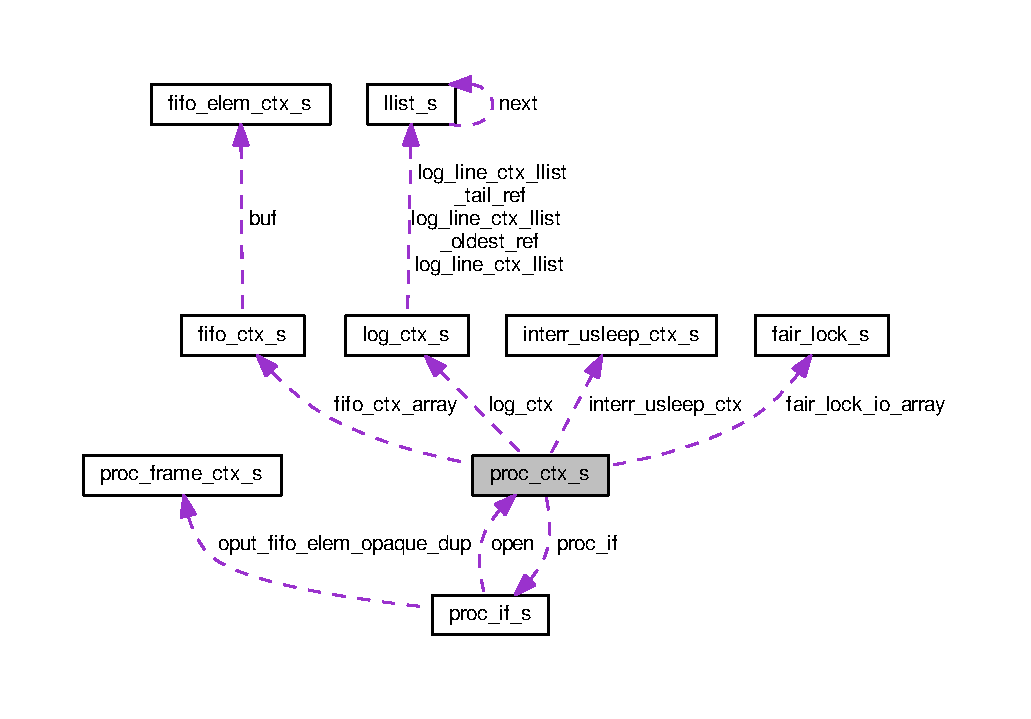
\includegraphics[width=350pt]{structproc__ctx__s__coll__graph}
\end{center}
\end{figure}
\subsection*{Public Attributes}
\begin{DoxyCompactItemize}
\item 
const \hyperlink{proc_8h_a679816cf30e0b7a8f3e7464e67a6a844}{proc\+\_\+if\+\_\+t} $\ast$ \hyperlink{structproc__ctx__s_ae63f720fef21f807ed42fe76806140f6}{proc\+\_\+if}
\item 
int \hyperlink{structproc__ctx__s_a3912d4b5eaffcdaefa00f149ca4a8c63}{proc\+\_\+instance\+\_\+index}
\item 
pthread\+\_\+mutex\+\_\+t \hyperlink{structproc__ctx__s_aea90c57d9b0a303b638a51ce7efa9a1e}{api\+\_\+mutex}
\item 
\hyperlink{structlog__ctx__s}{log\+\_\+ctx\+\_\+t} $\ast$ \hyperlink{structproc__ctx__s_a7c58dee78b4d7834e4c2fe430cd267d5}{log\+\_\+ctx}
\item 
\hyperlink{fifo_8c_acf3f21e64cbabccd8420c306740820c1}{fifo\+\_\+ctx\+\_\+t} $\ast$ \hyperlink{structproc__ctx__s_a3b71d039235f439a87d9ec7d7b5b5549}{fifo\+\_\+ctx\+\_\+array} \mbox{[}P\+R\+O\+C\+\_\+\+I\+O\+\_\+\+N\+UM\mbox{]}
\item 
\hyperlink{structfair__lock__s}{fair\+\_\+lock\+\_\+t} $\ast$ \hyperlink{structproc__ctx__s_a6529e1ba97566c429d658e121bb604bb}{fair\+\_\+lock\+\_\+io\+\_\+array} \mbox{[}P\+R\+O\+C\+\_\+\+I\+O\+\_\+\+N\+UM\mbox{]}
\item 
volatile int \hyperlink{structproc__ctx__s_a86a21b28f6c41f7a9a4cc9586f782d68}{flag\+\_\+exit}
\item 
pthread\+\_\+t \hyperlink{structproc__ctx__s_a09ad60355584215cfeb4d5589ee390b9}{proc\+\_\+thread}
\item 
const void $\ast$($\ast$ \hyperlink{structproc__ctx__s_a1149ce1c28aae8e553c85125e30be661}{start\+\_\+routine} )(void $\ast$)
\end{DoxyCompactItemize}
{\bf }\par
\begin{DoxyCompactItemize}
\item 
volatile uint32\+\_\+t \hyperlink{structproc__ctx__s_a31bad437eed5d81c08a01538416c3639}{bitrate} \mbox{[}P\+R\+O\+C\+\_\+\+I\+O\+\_\+\+N\+UM\mbox{]}
\item 
volatile uint32\+\_\+t {\bfseries acc\+\_\+io\+\_\+bits} \mbox{[}P\+R\+O\+C\+\_\+\+I\+O\+\_\+\+N\+UM\mbox{]}\hypertarget{structproc__ctx__s_a63e59dc7c4a361ca2b52e2354f51c33a}{}\label{structproc__ctx__s_a63e59dc7c4a361ca2b52e2354f51c33a}

\item 
pthread\+\_\+mutex\+\_\+t {\bfseries acc\+\_\+io\+\_\+bits\+\_\+mutex} \mbox{[}P\+R\+O\+C\+\_\+\+I\+O\+\_\+\+N\+UM\mbox{]}\hypertarget{structproc__ctx__s_a486d5806453d8171e298c449c6391c1d}{}\label{structproc__ctx__s_a486d5806453d8171e298c449c6391c1d}

\end{DoxyCompactItemize}

{\bf }\par
\begin{DoxyCompactItemize}
\item 
int64\+\_\+t {\bfseries iput\+\_\+pts\+\_\+array} \mbox{[}2\mbox{]}\mbox{[}\hyperlink{proc_8h_af53db00bc88282285037381807cc5c1d}{I\+P\+U\+T\+\_\+\+P\+T\+S\+\_\+\+A\+R\+R\+A\+Y\+\_\+\+S\+I\+ZE}\mbox{]}\hypertarget{structproc__ctx__s_afe00d8671976a864711e0db2841c5964}{}\label{structproc__ctx__s_afe00d8671976a864711e0db2841c5964}

\item 
volatile int {\bfseries iput\+\_\+pts\+\_\+array\+\_\+idx}\hypertarget{structproc__ctx__s_a143dc31fd44936ccafe2ecdaeef20ad6}{}\label{structproc__ctx__s_a143dc31fd44936ccafe2ecdaeef20ad6}

\end{DoxyCompactItemize}

{\bf }\par
\begin{DoxyCompactItemize}
\item 
volatile int64\+\_\+t \hyperlink{structproc__ctx__s_acdd3cc73dadcf7eb7c70c6e5ffb53293}{latency\+\_\+avg\+\_\+usec}
\item 
volatile int64\+\_\+t {\bfseries latency\+\_\+max\+\_\+usec}\hypertarget{structproc__ctx__s_a5cbe8711ddd1b36a2b203cfc8ef1b01f}{}\label{structproc__ctx__s_a5cbe8711ddd1b36a2b203cfc8ef1b01f}

\item 
volatile int64\+\_\+t {\bfseries latency\+\_\+min\+\_\+usec}\hypertarget{structproc__ctx__s_a0546eedba9aabcc7edc958f1ccc8cd42}{}\label{structproc__ctx__s_a0546eedba9aabcc7edc958f1ccc8cd42}

\item 
volatile int64\+\_\+t {\bfseries acc\+\_\+latency\+\_\+nsec}\hypertarget{structproc__ctx__s_a58e7e20b896b1d74789f2fe9b971fd09}{}\label{structproc__ctx__s_a58e7e20b896b1d74789f2fe9b971fd09}

\item 
volatile int {\bfseries acc\+\_\+latency\+\_\+cnt}\hypertarget{structproc__ctx__s_a3dea6eaed00798ceac47451e5923dc41}{}\label{structproc__ctx__s_a3dea6eaed00798ceac47451e5923dc41}

\item 
pthread\+\_\+mutex\+\_\+t {\bfseries latency\+\_\+mutex}\hypertarget{structproc__ctx__s_ac9705b88786b067a17f84178d52bbce1}{}\label{structproc__ctx__s_ac9705b88786b067a17f84178d52bbce1}

\end{DoxyCompactItemize}

{\bf }\par
\begin{DoxyCompactItemize}
\item 
\hyperlink{interr__usleep_8c_a952a138df6a0c053aa91d931c6c7de57}{interr\+\_\+usleep\+\_\+ctx\+\_\+t} $\ast$ \hyperlink{structproc__ctx__s_ae60a995d574f7f3e1719439b77ea02f9}{interr\+\_\+usleep\+\_\+ctx}
\item 
pthread\+\_\+t \hyperlink{structproc__ctx__s_a9cd9d87dfa63404f23d5571feaefcb71}{stats\+\_\+thread}
\end{DoxyCompactItemize}



\subsection{Detailed Description}
Generic processor (P\+R\+OC) context structure. 

Definition at line 85 of file proc.\+h.



\subsection{Member Data Documentation}
\index{proc\+\_\+ctx\+\_\+s@{proc\+\_\+ctx\+\_\+s}!api\+\_\+mutex@{api\+\_\+mutex}}
\index{api\+\_\+mutex@{api\+\_\+mutex}!proc\+\_\+ctx\+\_\+s@{proc\+\_\+ctx\+\_\+s}}
\subsubsection[{\texorpdfstring{api\+\_\+mutex}{api_mutex}}]{\setlength{\rightskip}{0pt plus 5cm}pthread\+\_\+mutex\+\_\+t proc\+\_\+ctx\+\_\+s\+::api\+\_\+mutex}\hypertarget{structproc__ctx__s_aea90c57d9b0a303b638a51ce7efa9a1e}{}\label{structproc__ctx__s_aea90c57d9b0a303b638a51ce7efa9a1e}
Processor A\+PI mutual exclusion lock. 

Definition at line 99 of file proc.\+h.

\index{proc\+\_\+ctx\+\_\+s@{proc\+\_\+ctx\+\_\+s}!bitrate@{bitrate}}
\index{bitrate@{bitrate}!proc\+\_\+ctx\+\_\+s@{proc\+\_\+ctx\+\_\+s}}
\subsubsection[{\texorpdfstring{bitrate}{bitrate}}]{\setlength{\rightskip}{0pt plus 5cm}volatile uint32\+\_\+t proc\+\_\+ctx\+\_\+s\+::bitrate\mbox{[}P\+R\+O\+C\+\_\+\+I\+O\+\_\+\+N\+UM\mbox{]}}\hypertarget{structproc__ctx__s_a31bad437eed5d81c08a01538416c3639}{}\label{structproc__ctx__s_a31bad437eed5d81c08a01538416c3639}
Bitrate measurement related variables\+:
\begin{DoxyItemize}
\item Input/output bitrate statistics \mbox{[}bits per second\mbox{]};
\item Accumulated bits at input/output interface. These variables are used internally to compute the input and output bitrate statistics periodically;
\item Critical region to acquire or modify \textquotesingle{}acc\+\_\+io\+\_\+bits\mbox{[}\mbox{]}\textquotesingle{} variable field. 
\end{DoxyItemize}

Definition at line 121 of file proc.\+h.

\index{proc\+\_\+ctx\+\_\+s@{proc\+\_\+ctx\+\_\+s}!fair\+\_\+lock\+\_\+io\+\_\+array@{fair\+\_\+lock\+\_\+io\+\_\+array}}
\index{fair\+\_\+lock\+\_\+io\+\_\+array@{fair\+\_\+lock\+\_\+io\+\_\+array}!proc\+\_\+ctx\+\_\+s@{proc\+\_\+ctx\+\_\+s}}
\subsubsection[{\texorpdfstring{fair\+\_\+lock\+\_\+io\+\_\+array}{fair_lock_io_array}}]{\setlength{\rightskip}{0pt plus 5cm}{\bf fair\+\_\+lock\+\_\+t}$\ast$ proc\+\_\+ctx\+\_\+s\+::fair\+\_\+lock\+\_\+io\+\_\+array\mbox{[}P\+R\+O\+C\+\_\+\+I\+O\+\_\+\+N\+UM\mbox{]}}\hypertarget{structproc__ctx__s_a6529e1ba97566c429d658e121bb604bb}{}\label{structproc__ctx__s_a6529e1ba97566c429d658e121bb604bb}
Input/output mutual exclusion locks. 

Definition at line 111 of file proc.\+h.

\index{proc\+\_\+ctx\+\_\+s@{proc\+\_\+ctx\+\_\+s}!fifo\+\_\+ctx\+\_\+array@{fifo\+\_\+ctx\+\_\+array}}
\index{fifo\+\_\+ctx\+\_\+array@{fifo\+\_\+ctx\+\_\+array}!proc\+\_\+ctx\+\_\+s@{proc\+\_\+ctx\+\_\+s}}
\subsubsection[{\texorpdfstring{fifo\+\_\+ctx\+\_\+array}{fifo_ctx_array}}]{\setlength{\rightskip}{0pt plus 5cm}{\bf fifo\+\_\+ctx\+\_\+t}$\ast$ proc\+\_\+ctx\+\_\+s\+::fifo\+\_\+ctx\+\_\+array\mbox{[}P\+R\+O\+C\+\_\+\+I\+O\+\_\+\+N\+UM\mbox{]}}\hypertarget{structproc__ctx__s_a3b71d039235f439a87d9ec7d7b5b5549}{}\label{structproc__ctx__s_a3b71d039235f439a87d9ec7d7b5b5549}
Input/output F\+I\+FO buffers. 

Definition at line 107 of file proc.\+h.

\index{proc\+\_\+ctx\+\_\+s@{proc\+\_\+ctx\+\_\+s}!flag\+\_\+exit@{flag\+\_\+exit}}
\index{flag\+\_\+exit@{flag\+\_\+exit}!proc\+\_\+ctx\+\_\+s@{proc\+\_\+ctx\+\_\+s}}
\subsubsection[{\texorpdfstring{flag\+\_\+exit}{flag_exit}}]{\setlength{\rightskip}{0pt plus 5cm}volatile int proc\+\_\+ctx\+\_\+s\+::flag\+\_\+exit}\hypertarget{structproc__ctx__s_a86a21b28f6c41f7a9a4cc9586f782d68}{}\label{structproc__ctx__s_a86a21b28f6c41f7a9a4cc9586f782d68}
Processing thread exit indicator. Set to non-\/zero to signal processing to abort immediately. 

Definition at line 169 of file proc.\+h.

\index{proc\+\_\+ctx\+\_\+s@{proc\+\_\+ctx\+\_\+s}!interr\+\_\+usleep\+\_\+ctx@{interr\+\_\+usleep\+\_\+ctx}}
\index{interr\+\_\+usleep\+\_\+ctx@{interr\+\_\+usleep\+\_\+ctx}!proc\+\_\+ctx\+\_\+s@{proc\+\_\+ctx\+\_\+s}}
\subsubsection[{\texorpdfstring{interr\+\_\+usleep\+\_\+ctx}{interr_usleep_ctx}}]{\setlength{\rightskip}{0pt plus 5cm}{\bf interr\+\_\+usleep\+\_\+ctx\+\_\+t}$\ast$ proc\+\_\+ctx\+\_\+s\+::interr\+\_\+usleep\+\_\+ctx}\hypertarget{structproc__ctx__s_ae60a995d574f7f3e1719439b77ea02f9}{}\label{structproc__ctx__s_ae60a995d574f7f3e1719439b77ea02f9}
Interruptible u-\/sleep used for periodical statistics thread. 

Definition at line 159 of file proc.\+h.

\index{proc\+\_\+ctx\+\_\+s@{proc\+\_\+ctx\+\_\+s}!latency\+\_\+avg\+\_\+usec@{latency\+\_\+avg\+\_\+usec}}
\index{latency\+\_\+avg\+\_\+usec@{latency\+\_\+avg\+\_\+usec}!proc\+\_\+ctx\+\_\+s@{proc\+\_\+ctx\+\_\+s}}
\subsubsection[{\texorpdfstring{latency\+\_\+avg\+\_\+usec}{latency_avg_usec}}]{\setlength{\rightskip}{0pt plus 5cm}volatile int64\+\_\+t proc\+\_\+ctx\+\_\+s\+::latency\+\_\+avg\+\_\+usec}\hypertarget{structproc__ctx__s_acdd3cc73dadcf7eb7c70c6e5ffb53293}{}\label{structproc__ctx__s_acdd3cc73dadcf7eb7c70c6e5ffb53293}
Latency measurement related variables.
\begin{DoxyItemize}
\item Average latency statistic \mbox{[}microseconds/second\mbox{]} (average value computed in a one-\/second period);
\item Accumulated latency value (addition of individual frame latencies in the average period);
\item Average counter (number of values that are added, used to compute average value);
\item Critical region to acquire or modify these field. 
\end{DoxyItemize}

Definition at line 148 of file proc.\+h.

\index{proc\+\_\+ctx\+\_\+s@{proc\+\_\+ctx\+\_\+s}!log\+\_\+ctx@{log\+\_\+ctx}}
\index{log\+\_\+ctx@{log\+\_\+ctx}!proc\+\_\+ctx\+\_\+s@{proc\+\_\+ctx\+\_\+s}}
\subsubsection[{\texorpdfstring{log\+\_\+ctx}{log_ctx}}]{\setlength{\rightskip}{0pt plus 5cm}{\bf log\+\_\+ctx\+\_\+t}$\ast$ proc\+\_\+ctx\+\_\+s\+::log\+\_\+ctx}\hypertarget{structproc__ctx__s_a7c58dee78b4d7834e4c2fe430cd267d5}{}\label{structproc__ctx__s_a7c58dee78b4d7834e4c2fe430cd267d5}
External L\+OG module context structure instance. 

Definition at line 103 of file proc.\+h.

\index{proc\+\_\+ctx\+\_\+s@{proc\+\_\+ctx\+\_\+s}!proc\+\_\+if@{proc\+\_\+if}}
\index{proc\+\_\+if@{proc\+\_\+if}!proc\+\_\+ctx\+\_\+s@{proc\+\_\+ctx\+\_\+s}}
\subsubsection[{\texorpdfstring{proc\+\_\+if}{proc_if}}]{\setlength{\rightskip}{0pt plus 5cm}const {\bf proc\+\_\+if\+\_\+t}$\ast$ proc\+\_\+ctx\+\_\+s\+::proc\+\_\+if}\hypertarget{structproc__ctx__s_ae63f720fef21f807ed42fe76806140f6}{}\label{structproc__ctx__s_ae63f720fef21f807ed42fe76806140f6}
P\+R\+OC interface structure. 

Definition at line 89 of file proc.\+h.

\index{proc\+\_\+ctx\+\_\+s@{proc\+\_\+ctx\+\_\+s}!proc\+\_\+instance\+\_\+index@{proc\+\_\+instance\+\_\+index}}
\index{proc\+\_\+instance\+\_\+index@{proc\+\_\+instance\+\_\+index}!proc\+\_\+ctx\+\_\+s@{proc\+\_\+ctx\+\_\+s}}
\subsubsection[{\texorpdfstring{proc\+\_\+instance\+\_\+index}{proc_instance_index}}]{\setlength{\rightskip}{0pt plus 5cm}int proc\+\_\+ctx\+\_\+s\+::proc\+\_\+instance\+\_\+index}\hypertarget{structproc__ctx__s_a3912d4b5eaffcdaefa00f149ca4a8c63}{}\label{structproc__ctx__s_a3912d4b5eaffcdaefa00f149ca4a8c63}
Each P\+R\+OC instance is registered in an instance array with a specific index. The idea behind using an array is to fetch as fast as possible the P\+R\+OC instance to perform i/o operations. 

Definition at line 95 of file proc.\+h.

\index{proc\+\_\+ctx\+\_\+s@{proc\+\_\+ctx\+\_\+s}!proc\+\_\+thread@{proc\+\_\+thread}}
\index{proc\+\_\+thread@{proc\+\_\+thread}!proc\+\_\+ctx\+\_\+s@{proc\+\_\+ctx\+\_\+s}}
\subsubsection[{\texorpdfstring{proc\+\_\+thread}{proc_thread}}]{\setlength{\rightskip}{0pt plus 5cm}pthread\+\_\+t proc\+\_\+ctx\+\_\+s\+::proc\+\_\+thread}\hypertarget{structproc__ctx__s_a09ad60355584215cfeb4d5589ee390b9}{}\label{structproc__ctx__s_a09ad60355584215cfeb4d5589ee390b9}
Processing thread. 

Definition at line 173 of file proc.\+h.

\index{proc\+\_\+ctx\+\_\+s@{proc\+\_\+ctx\+\_\+s}!start\+\_\+routine@{start\+\_\+routine}}
\index{start\+\_\+routine@{start\+\_\+routine}!proc\+\_\+ctx\+\_\+s@{proc\+\_\+ctx\+\_\+s}}
\subsubsection[{\texorpdfstring{start\+\_\+routine}{start_routine}}]{\setlength{\rightskip}{0pt plus 5cm}const void$\ast$($\ast$ proc\+\_\+ctx\+\_\+s\+::start\+\_\+routine) (void $\ast$)}\hypertarget{structproc__ctx__s_a1149ce1c28aae8e553c85125e30be661}{}\label{structproc__ctx__s_a1149ce1c28aae8e553c85125e30be661}
Processing thread function reference. It is initialized to point to the predefined module internal processing function \textquotesingle{}proc\+\_\+thr()\textquotesingle{} by default. Nevertheless, this pointer can be rewritten by any specific implementation in the \textquotesingle{}\hyperlink{structproc__if__s_a34999576771394dfb721463c8455ba06}{proc\+\_\+if\+\_\+s\+::open()}\textquotesingle{} callback. 

Definition at line 181 of file proc.\+h.

\index{proc\+\_\+ctx\+\_\+s@{proc\+\_\+ctx\+\_\+s}!stats\+\_\+thread@{stats\+\_\+thread}}
\index{stats\+\_\+thread@{stats\+\_\+thread}!proc\+\_\+ctx\+\_\+s@{proc\+\_\+ctx\+\_\+s}}
\subsubsection[{\texorpdfstring{stats\+\_\+thread}{stats_thread}}]{\setlength{\rightskip}{0pt plus 5cm}pthread\+\_\+t proc\+\_\+ctx\+\_\+s\+::stats\+\_\+thread}\hypertarget{structproc__ctx__s_a9cd9d87dfa63404f23d5571feaefcb71}{}\label{structproc__ctx__s_a9cd9d87dfa63404f23d5571feaefcb71}
Statistics thread. 

Definition at line 163 of file proc.\+h.



The documentation for this struct was generated from the following file\+:\begin{DoxyCompactItemize}
\item 
\hyperlink{proc_8h}{proc.\+h}\end{DoxyCompactItemize}

\input{structproc__frame__ctx__s}
\hypertarget{structproc__if__s}{}\section{proc\+\_\+if\+\_\+s Struct Reference}
\label{structproc__if__s}\index{proc\+\_\+if\+\_\+s@{proc\+\_\+if\+\_\+s}}


{\ttfamily \#include $<$proc\+\_\+if.\+h$>$}



Collaboration diagram for proc\+\_\+if\+\_\+s\+:\nopagebreak
\begin{figure}[H]
\begin{center}
\leavevmode
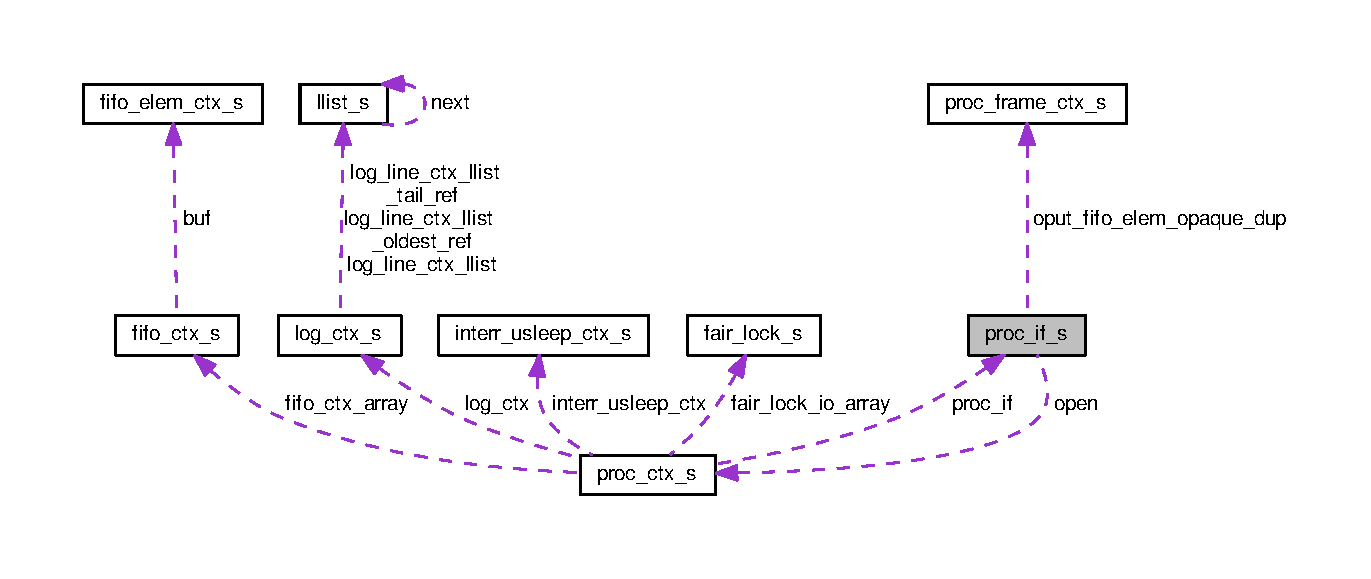
\includegraphics[width=350pt]{structproc__if__s__coll__graph}
\end{center}
\end{figure}
\subsection*{Public Attributes}
\begin{DoxyCompactItemize}
\item 
const char $\ast$ \hyperlink{structproc__if__s_aa284f1d0bdde2fae0b51101f658430ee}{proc\+\_\+name}
\item 
const char $\ast$ \hyperlink{structproc__if__s_a3a8a04d2e81ca4dfa55a8526644dd729}{proc\+\_\+type}
\item 
const char $\ast$ \hyperlink{structproc__if__s_afdb204f8c976ed829466774aaa6cdf89}{proc\+\_\+mime}
\item 
uint64\+\_\+t \hyperlink{structproc__if__s_a657d976a32c34bff11070599b11c2dd7}{flag\+\_\+proc\+\_\+features}
\item 
\hyperlink{proc_8h_ae264f89be30fc03f5053bc16d58cba05}{proc\+\_\+ctx\+\_\+t} $\ast$($\ast$ \hyperlink{structproc__if__s_a34999576771394dfb721463c8455ba06}{open} )(const \hyperlink{proc_8h_a679816cf30e0b7a8f3e7464e67a6a844}{proc\+\_\+if\+\_\+t} $\ast$proc\+\_\+if, const char $\ast$settings\+\_\+str, \hyperlink{structlog__ctx__s}{log\+\_\+ctx\+\_\+t} $\ast$log\+\_\+ctx, va\+\_\+list arg)
\item 
void($\ast$ \hyperlink{structproc__if__s_af5971ac1d09d1c6ec3508c36fb286c19}{close} )(\hyperlink{proc_8h_ae264f89be30fc03f5053bc16d58cba05}{proc\+\_\+ctx\+\_\+t} $\ast$$\ast$ref\+\_\+proc\+\_\+ctx)
\item 
int($\ast$ \hyperlink{structproc__if__s_a0393cc5e598e19951d447a926c364e3f}{send\+\_\+frame} )(\hyperlink{proc_8h_ae264f89be30fc03f5053bc16d58cba05}{proc\+\_\+ctx\+\_\+t} $\ast$proc\+\_\+ctx, const \hyperlink{structproc__frame__ctx__s}{proc\+\_\+frame\+\_\+ctx\+\_\+t} $\ast$proc\+\_\+frame\+\_\+ctx)
\item 
int($\ast$ {\bfseries send\+\_\+frame\+\_\+nodup} )(\hyperlink{proc_8h_ae264f89be30fc03f5053bc16d58cba05}{proc\+\_\+ctx\+\_\+t} $\ast$proc\+\_\+ctx, \hyperlink{structproc__frame__ctx__s}{proc\+\_\+frame\+\_\+ctx\+\_\+t} $\ast$$\ast$ref\+\_\+proc\+\_\+frame\+\_\+ctx)\hypertarget{structproc__if__s_af460a3b26b0717140cc08014b6c63191}{}\label{structproc__if__s_af460a3b26b0717140cc08014b6c63191}

\item 
int($\ast$ \hyperlink{structproc__if__s_a43115b2b1fa63fbfca191c18f28f2fea}{recv\+\_\+frame} )(\hyperlink{proc_8h_ae264f89be30fc03f5053bc16d58cba05}{proc\+\_\+ctx\+\_\+t} $\ast$proc\+\_\+ctx, \hyperlink{structproc__frame__ctx__s}{proc\+\_\+frame\+\_\+ctx\+\_\+t} $\ast$$\ast$ref\+\_\+proc\+\_\+frame\+\_\+ctx)
\item 
int($\ast$ \hyperlink{structproc__if__s_a19d63c8db2cbfb227134f5a5bd5c8561}{unblock} )(\hyperlink{proc_8h_ae264f89be30fc03f5053bc16d58cba05}{proc\+\_\+ctx\+\_\+t} $\ast$proc\+\_\+ctx)
\item 
int($\ast$ \hyperlink{structproc__if__s_acb4d2c240c52904ebd6904f54b1a9b78}{rest\+\_\+put} )(\hyperlink{proc_8h_ae264f89be30fc03f5053bc16d58cba05}{proc\+\_\+ctx\+\_\+t} $\ast$proc\+\_\+ctx, const char $\ast$str)
\item 
int($\ast$ \hyperlink{structproc__if__s_a1e45b33c52b931954f7a0d8a14f0db53}{rest\+\_\+get} )(\hyperlink{proc_8h_ae264f89be30fc03f5053bc16d58cba05}{proc\+\_\+ctx\+\_\+t} $\ast$proc\+\_\+ctx, const \hyperlink{proc__if_8h_a9bea3dae53a91f2a3e3a459d1d3e22b3}{proc\+\_\+if\+\_\+rest\+\_\+fmt\+\_\+t} rest\+\_\+fmt, void $\ast$$\ast$ref\+\_\+reponse)
\item 
int($\ast$ \hyperlink{structproc__if__s_ab67b4061f94b6f15ae40c796b6b33597}{process\+\_\+frame} )(\hyperlink{proc_8h_ae264f89be30fc03f5053bc16d58cba05}{proc\+\_\+ctx\+\_\+t} $\ast$proc\+\_\+ctx, \hyperlink{fifo_8c_acf3f21e64cbabccd8420c306740820c1}{fifo\+\_\+ctx\+\_\+t} $\ast$fifo\+\_\+ctx\+\_\+iput, \hyperlink{fifo_8c_acf3f21e64cbabccd8420c306740820c1}{fifo\+\_\+ctx\+\_\+t} $\ast$fifo\+\_\+ctx\+\_\+oput)
\item 
int($\ast$ \hyperlink{structproc__if__s_a4ca0939d6721f368d2560851197fca36}{opt} )(\hyperlink{proc_8h_ae264f89be30fc03f5053bc16d58cba05}{proc\+\_\+ctx\+\_\+t} $\ast$proc\+\_\+ctx, const char $\ast$tag, va\+\_\+list arg)
\item 
void $\ast$($\ast$ \hyperlink{structproc__if__s_a558cec57df436699d4154775894f2313}{iput\+\_\+fifo\+\_\+elem\+\_\+opaque\+\_\+dup} )(const \hyperlink{structproc__frame__ctx__s}{proc\+\_\+frame\+\_\+ctx\+\_\+t} $\ast$proc\+\_\+frame\+\_\+ctx)
\item 
void($\ast$ \hyperlink{structproc__if__s_aec3bf948ff945ac2f5a4c834ea3b57da}{iput\+\_\+fifo\+\_\+elem\+\_\+opaque\+\_\+release} )(void $\ast$$\ast$ref\+\_\+t)
\item 
\hyperlink{structproc__frame__ctx__s}{proc\+\_\+frame\+\_\+ctx\+\_\+t} $\ast$($\ast$ \hyperlink{structproc__if__s_a7806bbda25988d9ee54f6d0bb143c697}{oput\+\_\+fifo\+\_\+elem\+\_\+opaque\+\_\+dup} )(const void $\ast$t)
\end{DoxyCompactItemize}


\subsection{Detailed Description}
P\+R\+OC interface structure prototype. Each P\+R\+OC type will define a static and unambiguous interface of this type. 

Definition at line 169 of file proc\+\_\+if.\+h.



\subsection{Member Data Documentation}
\index{proc\+\_\+if\+\_\+s@{proc\+\_\+if\+\_\+s}!close@{close}}
\index{close@{close}!proc\+\_\+if\+\_\+s@{proc\+\_\+if\+\_\+s}}
\subsubsection[{\texorpdfstring{close}{close}}]{\setlength{\rightskip}{0pt plus 5cm}void($\ast$ proc\+\_\+if\+\_\+s\+::close) ({\bf proc\+\_\+ctx\+\_\+t} $\ast$$\ast$ref\+\_\+proc\+\_\+ctx)}\hypertarget{structproc__if__s_af5971ac1d09d1c6ec3508c36fb286c19}{}\label{structproc__if__s_af5971ac1d09d1c6ec3508c36fb286c19}
Ends processing thread, de-\/initialize and release the processor (P\+R\+OC) context structure and all the related resources. This callback is mandatory (cannot be N\+U\+LL). 
\begin{DoxyParams}{Parameters}
{\em ref\+\_\+proc\+\_\+ctx} & Reference to the pointer to the processor (P\+R\+OC) context structure to be release, that was obtained in a previous call to the \textquotesingle{}\hyperlink{structproc__if__s_a34999576771394dfb721463c8455ba06}{open()}\textquotesingle{} callback method. Pointer is set to N\+U\+LL on return. \\
\hline
\end{DoxyParams}


Definition at line 217 of file proc\+\_\+if.\+h.

\index{proc\+\_\+if\+\_\+s@{proc\+\_\+if\+\_\+s}!flag\+\_\+proc\+\_\+features@{flag\+\_\+proc\+\_\+features}}
\index{flag\+\_\+proc\+\_\+features@{flag\+\_\+proc\+\_\+features}!proc\+\_\+if\+\_\+s@{proc\+\_\+if\+\_\+s}}
\subsubsection[{\texorpdfstring{flag\+\_\+proc\+\_\+features}{flag_proc_features}}]{\setlength{\rightskip}{0pt plus 5cm}uint64\+\_\+t proc\+\_\+if\+\_\+s\+::flag\+\_\+proc\+\_\+features}\hypertarget{structproc__if__s_a657d976a32c34bff11070599b11c2dd7}{}\label{structproc__if__s_a657d976a32c34bff11070599b11c2dd7}
Processor features flags. 

Definition at line 190 of file proc\+\_\+if.\+h.

\index{proc\+\_\+if\+\_\+s@{proc\+\_\+if\+\_\+s}!iput\+\_\+fifo\+\_\+elem\+\_\+opaque\+\_\+dup@{iput\+\_\+fifo\+\_\+elem\+\_\+opaque\+\_\+dup}}
\index{iput\+\_\+fifo\+\_\+elem\+\_\+opaque\+\_\+dup@{iput\+\_\+fifo\+\_\+elem\+\_\+opaque\+\_\+dup}!proc\+\_\+if\+\_\+s@{proc\+\_\+if\+\_\+s}}
\subsubsection[{\texorpdfstring{iput\+\_\+fifo\+\_\+elem\+\_\+opaque\+\_\+dup}{iput_fifo_elem_opaque_dup}}]{\setlength{\rightskip}{0pt plus 5cm}void$\ast$($\ast$ proc\+\_\+if\+\_\+s\+::iput\+\_\+fifo\+\_\+elem\+\_\+opaque\+\_\+dup) (const {\bf proc\+\_\+frame\+\_\+ctx\+\_\+t} $\ast$proc\+\_\+frame\+\_\+ctx)}\hypertarget{structproc__if__s_a558cec57df436699d4154775894f2313}{}\label{structproc__if__s_a558cec57df436699d4154775894f2313}
This callback is registered in the F\+I\+FO management A\+PI and is used to internally duplicate the input frame structure when it is pushed to the processor input F\+I\+FO. Typically, this callback is used to transform the input type proc\+\_\+frame\+\_\+ctx\+\_\+t to another structure type that will be actually allocated in the F\+I\+FO. This callback is optional, and can be set to N\+U\+LL. In that case, the processor input frame structure is assumed to be of type proc\+\_\+frame\+\_\+ctx\+\_\+t (thus will be duplicated using function \textquotesingle{}\hyperlink{proc__if_8c_a26df07b260850afd03ec73572608a034}{proc\+\_\+frame\+\_\+ctx\+\_\+allocate()}\textquotesingle{}). 
\begin{DoxyParams}{Parameters}
{\em proc\+\_\+frame\+\_\+ctx} & Processor frame context structure (see proc\+\_\+frame\+\_\+ctx\+\_\+t). return Opaque structure (can be private format) duplicating the input frame. This structure will be pushed to the processor input F\+I\+FO. \\
\hline
\end{DoxyParams}


Definition at line 311 of file proc\+\_\+if.\+h.

\index{proc\+\_\+if\+\_\+s@{proc\+\_\+if\+\_\+s}!iput\+\_\+fifo\+\_\+elem\+\_\+opaque\+\_\+release@{iput\+\_\+fifo\+\_\+elem\+\_\+opaque\+\_\+release}}
\index{iput\+\_\+fifo\+\_\+elem\+\_\+opaque\+\_\+release@{iput\+\_\+fifo\+\_\+elem\+\_\+opaque\+\_\+release}!proc\+\_\+if\+\_\+s@{proc\+\_\+if\+\_\+s}}
\subsubsection[{\texorpdfstring{iput\+\_\+fifo\+\_\+elem\+\_\+opaque\+\_\+release}{iput_fifo_elem_opaque_release}}]{\setlength{\rightskip}{0pt plus 5cm}void($\ast$ proc\+\_\+if\+\_\+s\+::iput\+\_\+fifo\+\_\+elem\+\_\+opaque\+\_\+release) (void $\ast$$\ast$ref\+\_\+t)}\hypertarget{structproc__if__s_aec3bf948ff945ac2f5a4c834ea3b57da}{}\label{structproc__if__s_aec3bf948ff945ac2f5a4c834ea3b57da}
This callback is registered in the F\+I\+FO management A\+PI and is complementary to the callback \textquotesingle{}\hyperlink{structproc__if__s_a558cec57df436699d4154775894f2313}{iput\+\_\+fifo\+\_\+elem\+\_\+opaque\+\_\+dup()}\textquotesingle{}\+: it is the function used to release the elements duplicated and stored in the processor input F\+I\+FO using \textquotesingle{}\hyperlink{structproc__if__s_a558cec57df436699d4154775894f2313}{iput\+\_\+fifo\+\_\+elem\+\_\+opaque\+\_\+dup()}\textquotesingle{}. This callback is optional, and can be set to N\+U\+LL. In that case, the processor input frame structure is assumed to be of type proc\+\_\+frame\+\_\+ctx\+\_\+t (thus will be released using function \textquotesingle{}\hyperlink{proc__if_8c_afad6906a6da22ba369b736863c1e204e}{proc\+\_\+frame\+\_\+ctx\+\_\+release()}\textquotesingle{}). 
\begin{DoxyParams}{Parameters}
{\em ref\+\_\+t} & Opaque reference to a pointer to the structure type to be released. \\
\hline
\end{DoxyParams}


Definition at line 324 of file proc\+\_\+if.\+h.

\index{proc\+\_\+if\+\_\+s@{proc\+\_\+if\+\_\+s}!open@{open}}
\index{open@{open}!proc\+\_\+if\+\_\+s@{proc\+\_\+if\+\_\+s}}
\subsubsection[{\texorpdfstring{open}{open}}]{\setlength{\rightskip}{0pt plus 5cm}{\bf proc\+\_\+ctx\+\_\+t}$\ast$($\ast$ proc\+\_\+if\+\_\+s\+::open) (const {\bf proc\+\_\+if\+\_\+t} $\ast$proc\+\_\+if, const char $\ast$settings\+\_\+str, {\bf log\+\_\+ctx\+\_\+t} $\ast$log\+\_\+ctx, va\+\_\+list arg)}\hypertarget{structproc__if__s_a34999576771394dfb721463c8455ba06}{}\label{structproc__if__s_a34999576771394dfb721463c8455ba06}
Allocates specific processor (P\+R\+OC) context structure, initializes, and launches processing thread. This callback is mandatory (cannot be N\+U\+LL). 
\begin{DoxyParams}{Parameters}
{\em proc\+\_\+if} & Pointer to the processor interface structure (static and unambiguous interface of the type of processor we are opening). \\
\hline
{\em settings\+\_\+str} & Character string containing initial settings for the processor. String format can be either a query-\/string or J\+S\+ON. \\
\hline
{\em log\+\_\+ctx} & Pointer to the L\+OG module context structure. \\
\hline
{\em arg} & Variable list of parameters defined by user. \\
\hline
\end{DoxyParams}
\begin{DoxyReturn}{Returns}
Pointer to the processor context structure on success, N\+U\+LL if fails. 
\end{DoxyReturn}


Definition at line 207 of file proc\+\_\+if.\+h.

\index{proc\+\_\+if\+\_\+s@{proc\+\_\+if\+\_\+s}!opt@{opt}}
\index{opt@{opt}!proc\+\_\+if\+\_\+s@{proc\+\_\+if\+\_\+s}}
\subsubsection[{\texorpdfstring{opt}{opt}}]{\setlength{\rightskip}{0pt plus 5cm}int($\ast$ proc\+\_\+if\+\_\+s\+::opt) ({\bf proc\+\_\+ctx\+\_\+t} $\ast$proc\+\_\+ctx, const char $\ast$tag, va\+\_\+list arg)}\hypertarget{structproc__if__s_a4ca0939d6721f368d2560851197fca36}{}\label{structproc__if__s_a4ca0939d6721f368d2560851197fca36}
Request for specific processor options. This callback is optional (can be set to N\+U\+LL). 
\begin{DoxyParams}{Parameters}
{\em proc\+\_\+ctx} & Pointer to the processor (P\+R\+OC) context structure obtained in a previous call to the \textquotesingle{}\hyperlink{structproc__if__s_a34999576771394dfb721463c8455ba06}{open()}\textquotesingle{} callback method. \\
\hline
{\em tag} & Processor option tag, namely, option identifier string. Refer to the specific implementation of this function to see the available options. arg Variable list of parameters according to selected option. Refer to the specific implementation of this function to see the parameters corresponding to each available option. \\
\hline
\end{DoxyParams}
\begin{DoxyReturn}{Returns}
Status code (S\+T\+A\+T\+\_\+\+S\+U\+C\+C\+E\+SS code in case of success, for other code values please refer to .\hyperlink{stat__codes_8h}{stat\+\_\+codes.\+h}). 
\end{DoxyReturn}


Definition at line 295 of file proc\+\_\+if.\+h.

\index{proc\+\_\+if\+\_\+s@{proc\+\_\+if\+\_\+s}!oput\+\_\+fifo\+\_\+elem\+\_\+opaque\+\_\+dup@{oput\+\_\+fifo\+\_\+elem\+\_\+opaque\+\_\+dup}}
\index{oput\+\_\+fifo\+\_\+elem\+\_\+opaque\+\_\+dup@{oput\+\_\+fifo\+\_\+elem\+\_\+opaque\+\_\+dup}!proc\+\_\+if\+\_\+s@{proc\+\_\+if\+\_\+s}}
\subsubsection[{\texorpdfstring{oput\+\_\+fifo\+\_\+elem\+\_\+opaque\+\_\+dup}{oput_fifo_elem_opaque_dup}}]{\setlength{\rightskip}{0pt plus 5cm}{\bf proc\+\_\+frame\+\_\+ctx\+\_\+t}$\ast$($\ast$ proc\+\_\+if\+\_\+s\+::oput\+\_\+fifo\+\_\+elem\+\_\+opaque\+\_\+dup) (const void $\ast$t)}\hypertarget{structproc__if__s_a7806bbda25988d9ee54f6d0bb143c697}{}\label{structproc__if__s_a7806bbda25988d9ee54f6d0bb143c697}
This callback is registered in the F\+I\+FO management A\+PI and is used to internally duplicate the processor\textquotesingle{}s output frame structure when it is pushed into the processor output F\+I\+FO. Typically, this callback is used to transform the processor\textquotesingle{}s opaque output type to the type proc\+\_\+frame\+\_\+ctx\+\_\+t that will be actually allocated in the F\+I\+FO. This callback is optional, and can be set to N\+U\+LL. In that case, the processor output frame structure is assumed to be of type proc\+\_\+frame\+\_\+ctx\+\_\+t (thus will be duplicated using function \textquotesingle{}\hyperlink{proc__if_8c_a26df07b260850afd03ec73572608a034}{proc\+\_\+frame\+\_\+ctx\+\_\+allocate()}\textquotesingle{}). 
\begin{DoxyParams}{Parameters}
{\em t} & Opaque processor\textquotesingle{}s output frame structure. return Processor frame context structure (see proc\+\_\+frame\+\_\+ctx\+\_\+t). This structure will be pushed to the processor output F\+I\+FO. \\
\hline
\end{DoxyParams}


Definition at line 339 of file proc\+\_\+if.\+h.

\index{proc\+\_\+if\+\_\+s@{proc\+\_\+if\+\_\+s}!proc\+\_\+mime@{proc\+\_\+mime}}
\index{proc\+\_\+mime@{proc\+\_\+mime}!proc\+\_\+if\+\_\+s@{proc\+\_\+if\+\_\+s}}
\subsubsection[{\texorpdfstring{proc\+\_\+mime}{proc_mime}}]{\setlength{\rightskip}{0pt plus 5cm}const char$\ast$ proc\+\_\+if\+\_\+s\+::proc\+\_\+mime}\hypertarget{structproc__if__s_afdb204f8c976ed829466774aaa6cdf89}{}\label{structproc__if__s_afdb204f8c976ed829466774aaa6cdf89}
Media type and sub-\/type (formerly known as M\+I\+ME types and sub-\/type). See \href{http://www.iana.org/assignments/media-types/media-types.xhtml}{\tt http\+://www.\+iana.\+org/assignments/media-\/types/media-\/types.\+xhtml}. For muxers we use by default\+: \char`\"{}application/octet-\/stream\char`\"{} This field is mandatory (can not be set to N\+U\+LL). 

Definition at line 186 of file proc\+\_\+if.\+h.

\index{proc\+\_\+if\+\_\+s@{proc\+\_\+if\+\_\+s}!proc\+\_\+name@{proc\+\_\+name}}
\index{proc\+\_\+name@{proc\+\_\+name}!proc\+\_\+if\+\_\+s@{proc\+\_\+if\+\_\+s}}
\subsubsection[{\texorpdfstring{proc\+\_\+name}{proc_name}}]{\setlength{\rightskip}{0pt plus 5cm}const char$\ast$ proc\+\_\+if\+\_\+s\+::proc\+\_\+name}\hypertarget{structproc__if__s_aa284f1d0bdde2fae0b51101f658430ee}{}\label{structproc__if__s_aa284f1d0bdde2fae0b51101f658430ee}
Unambiguous P\+R\+OC identifier name (character string). This field is mandatory (can not be set to N\+U\+LL). 

Definition at line 174 of file proc\+\_\+if.\+h.

\index{proc\+\_\+if\+\_\+s@{proc\+\_\+if\+\_\+s}!proc\+\_\+type@{proc\+\_\+type}}
\index{proc\+\_\+type@{proc\+\_\+type}!proc\+\_\+if\+\_\+s@{proc\+\_\+if\+\_\+s}}
\subsubsection[{\texorpdfstring{proc\+\_\+type}{proc_type}}]{\setlength{\rightskip}{0pt plus 5cm}const char$\ast$ proc\+\_\+if\+\_\+s\+::proc\+\_\+type}\hypertarget{structproc__if__s_a3a8a04d2e81ca4dfa55a8526644dd729}{}\label{structproc__if__s_a3a8a04d2e81ca4dfa55a8526644dd729}
Processor type\+: encoder, decoder, multiplexer, demultiplexer. This field is mandatory (can not be set to N\+U\+LL). 

Definition at line 179 of file proc\+\_\+if.\+h.

\index{proc\+\_\+if\+\_\+s@{proc\+\_\+if\+\_\+s}!process\+\_\+frame@{process\+\_\+frame}}
\index{process\+\_\+frame@{process\+\_\+frame}!proc\+\_\+if\+\_\+s@{proc\+\_\+if\+\_\+s}}
\subsubsection[{\texorpdfstring{process\+\_\+frame}{process_frame}}]{\setlength{\rightskip}{0pt plus 5cm}int($\ast$ proc\+\_\+if\+\_\+s\+::process\+\_\+frame) ({\bf proc\+\_\+ctx\+\_\+t} $\ast$proc\+\_\+ctx, {\bf fifo\+\_\+ctx\+\_\+t} $\ast$fifo\+\_\+ctx\+\_\+iput, {\bf fifo\+\_\+ctx\+\_\+t} $\ast$fifo\+\_\+ctx\+\_\+oput)}\hypertarget{structproc__if__s_ab67b4061f94b6f15ae40c796b6b33597}{}\label{structproc__if__s_ab67b4061f94b6f15ae40c796b6b33597}
Process one frame of data. The frame is read from the input F\+I\+FO buffer and is completely processed. If an output frame is produced, is written to the output F\+I\+FO buffer. This callback is optional (can be set to N\+U\+LL). 
\begin{DoxyParams}{Parameters}
{\em proc\+\_\+ctx} & Pointer to the processor (P\+R\+OC) context structure obtained in a previous call to the \textquotesingle{}\hyperlink{structproc__if__s_a34999576771394dfb721463c8455ba06}{open()}\textquotesingle{} callback method. \\
\hline
{\em fifo\+\_\+ctx\+\_\+iput} & Pointer to the input F\+I\+FO buffer context structure. \\
\hline
{\em fifo\+\_\+ctx\+\_\+oput} & Pointer to the output F\+I\+FO buffer context structure. \\
\hline
\end{DoxyParams}
\begin{DoxyReturn}{Returns}
Status code (S\+T\+A\+T\+\_\+\+S\+U\+C\+C\+E\+SS code in case of success, for other code values please refer to .\hyperlink{stat__codes_8h}{stat\+\_\+codes.\+h}). 
\end{DoxyReturn}


Definition at line 279 of file proc\+\_\+if.\+h.

\index{proc\+\_\+if\+\_\+s@{proc\+\_\+if\+\_\+s}!recv\+\_\+frame@{recv\+\_\+frame}}
\index{recv\+\_\+frame@{recv\+\_\+frame}!proc\+\_\+if\+\_\+s@{proc\+\_\+if\+\_\+s}}
\subsubsection[{\texorpdfstring{recv\+\_\+frame}{recv_frame}}]{\setlength{\rightskip}{0pt plus 5cm}int($\ast$ proc\+\_\+if\+\_\+s\+::recv\+\_\+frame) ({\bf proc\+\_\+ctx\+\_\+t} $\ast$proc\+\_\+ctx, {\bf proc\+\_\+frame\+\_\+ctx\+\_\+t} $\ast$$\ast$ref\+\_\+proc\+\_\+frame\+\_\+ctx)}\hypertarget{structproc__if__s_a43115b2b1fa63fbfca191c18f28f2fea}{}\label{structproc__if__s_a43115b2b1fa63fbfca191c18f28f2fea}
//\+T\+O\+DO This callback is optional (can be set to N\+U\+LL). 

Definition at line 230 of file proc\+\_\+if.\+h.

\index{proc\+\_\+if\+\_\+s@{proc\+\_\+if\+\_\+s}!rest\+\_\+get@{rest\+\_\+get}}
\index{rest\+\_\+get@{rest\+\_\+get}!proc\+\_\+if\+\_\+s@{proc\+\_\+if\+\_\+s}}
\subsubsection[{\texorpdfstring{rest\+\_\+get}{rest_get}}]{\setlength{\rightskip}{0pt plus 5cm}int($\ast$ proc\+\_\+if\+\_\+s\+::rest\+\_\+get) ({\bf proc\+\_\+ctx\+\_\+t} $\ast$proc\+\_\+ctx, const {\bf proc\+\_\+if\+\_\+rest\+\_\+fmt\+\_\+t} rest\+\_\+fmt, void $\ast$$\ast$ref\+\_\+reponse)}\hypertarget{structproc__if__s_a1e45b33c52b931954f7a0d8a14f0db53}{}\label{structproc__if__s_a1e45b33c52b931954f7a0d8a14f0db53}
Get current processor (P\+R\+OC) settings. Settings are returned by argument in a character string in J\+S\+ON format. This method is asynchronous and thread safe. This callback is optional (can be set to N\+U\+LL). 
\begin{DoxyParams}{Parameters}
{\em proc\+\_\+ctx} & Pointer to the processor (P\+R\+OC) context structure obtained in a previous call to the \textquotesingle{}\hyperlink{structproc__if__s_a34999576771394dfb721463c8455ba06}{open()}\textquotesingle{} callback method. \\
\hline
{\em rest\+\_\+fmt} & Indicates the format in which the response data is to be returned. Available formats are enumerated at \textquotesingle{}proc\+\_\+if\+\_\+rest\+\_\+fmt\+\_\+t\textquotesingle{}. \\
\hline
{\em ref\+\_\+reponse} & Reference to the pointer to a data structure returning the processor\textquotesingle{}s representational state (including current settings). The returned data structure is formatted according to what is indicated in the parameter \textquotesingle{}rest\+\_\+fmt\textquotesingle{}. \\
\hline
\end{DoxyParams}
\begin{DoxyReturn}{Returns}
Status code (S\+T\+A\+T\+\_\+\+S\+U\+C\+C\+E\+SS code in case of success, for other code values please refer to .\hyperlink{stat__codes_8h}{stat\+\_\+codes.\+h}). 
\end{DoxyReturn}


Definition at line 265 of file proc\+\_\+if.\+h.

\index{proc\+\_\+if\+\_\+s@{proc\+\_\+if\+\_\+s}!rest\+\_\+put@{rest\+\_\+put}}
\index{rest\+\_\+put@{rest\+\_\+put}!proc\+\_\+if\+\_\+s@{proc\+\_\+if\+\_\+s}}
\subsubsection[{\texorpdfstring{rest\+\_\+put}{rest_put}}]{\setlength{\rightskip}{0pt plus 5cm}int($\ast$ proc\+\_\+if\+\_\+s\+::rest\+\_\+put) ({\bf proc\+\_\+ctx\+\_\+t} $\ast$proc\+\_\+ctx, const char $\ast$str)}\hypertarget{structproc__if__s_acb4d2c240c52904ebd6904f54b1a9b78}{}\label{structproc__if__s_acb4d2c240c52904ebd6904f54b1a9b78}
Put new processor (P\+R\+OC) settings. Parameters can be passed either as a query-\/string or J\+S\+ON. This method is asynchronous and thread safe. This callback is optional (can be set to N\+U\+LL). 
\begin{DoxyParams}{Parameters}
{\em proc\+\_\+ctx} & Pointer to the processor (P\+R\+OC) context structure obtained in a previous call to the \textquotesingle{}\hyperlink{structproc__if__s_a34999576771394dfb721463c8455ba06}{open()}\textquotesingle{} callback method. \\
\hline
{\em str} & Pointer to a character string containing new settings for the processor. String format can be either a query-\/string or J\+S\+ON. \\
\hline
\end{DoxyParams}
\begin{DoxyReturn}{Returns}
Status code (S\+T\+A\+T\+\_\+\+S\+U\+C\+C\+E\+SS code in case of success, for other code values please refer to .\hyperlink{stat__codes_8h}{stat\+\_\+codes.\+h}). 
\end{DoxyReturn}


Definition at line 248 of file proc\+\_\+if.\+h.

\index{proc\+\_\+if\+\_\+s@{proc\+\_\+if\+\_\+s}!send\+\_\+frame@{send\+\_\+frame}}
\index{send\+\_\+frame@{send\+\_\+frame}!proc\+\_\+if\+\_\+s@{proc\+\_\+if\+\_\+s}}
\subsubsection[{\texorpdfstring{send\+\_\+frame}{send_frame}}]{\setlength{\rightskip}{0pt plus 5cm}int($\ast$ proc\+\_\+if\+\_\+s\+::send\+\_\+frame) ({\bf proc\+\_\+ctx\+\_\+t} $\ast$proc\+\_\+ctx, const {\bf proc\+\_\+frame\+\_\+ctx\+\_\+t} $\ast$proc\+\_\+frame\+\_\+ctx)}\hypertarget{structproc__if__s_a0393cc5e598e19951d447a926c364e3f}{}\label{structproc__if__s_a0393cc5e598e19951d447a926c364e3f}
// T\+O\+DO This callback is optional (can be set to N\+U\+LL). 

Definition at line 222 of file proc\+\_\+if.\+h.

\index{proc\+\_\+if\+\_\+s@{proc\+\_\+if\+\_\+s}!unblock@{unblock}}
\index{unblock@{unblock}!proc\+\_\+if\+\_\+s@{proc\+\_\+if\+\_\+s}}
\subsubsection[{\texorpdfstring{unblock}{unblock}}]{\setlength{\rightskip}{0pt plus 5cm}int($\ast$ proc\+\_\+if\+\_\+s\+::unblock) ({\bf proc\+\_\+ctx\+\_\+t} $\ast$proc\+\_\+ctx)}\hypertarget{structproc__if__s_a19d63c8db2cbfb227134f5a5bd5c8561}{}\label{structproc__if__s_a19d63c8db2cbfb227134f5a5bd5c8561}
//\+T\+O\+DO 

Definition at line 235 of file proc\+\_\+if.\+h.



The documentation for this struct was generated from the following file\+:\begin{DoxyCompactItemize}
\item 
\hyperlink{proc__if_8h}{proc\+\_\+if.\+h}\end{DoxyCompactItemize}

\input{structproc__muxer__mux__ctx__s}
\input{structproc__sample__fmt__lut__s}
\hypertarget{structprocs__ctx__s}{}\section{procs\+\_\+ctx\+\_\+s Struct Reference}
\label{structprocs__ctx__s}\index{procs\+\_\+ctx\+\_\+s@{procs\+\_\+ctx\+\_\+s}}


Collaboration diagram for procs\+\_\+ctx\+\_\+s\+:\nopagebreak
\begin{figure}[H]
\begin{center}
\leavevmode
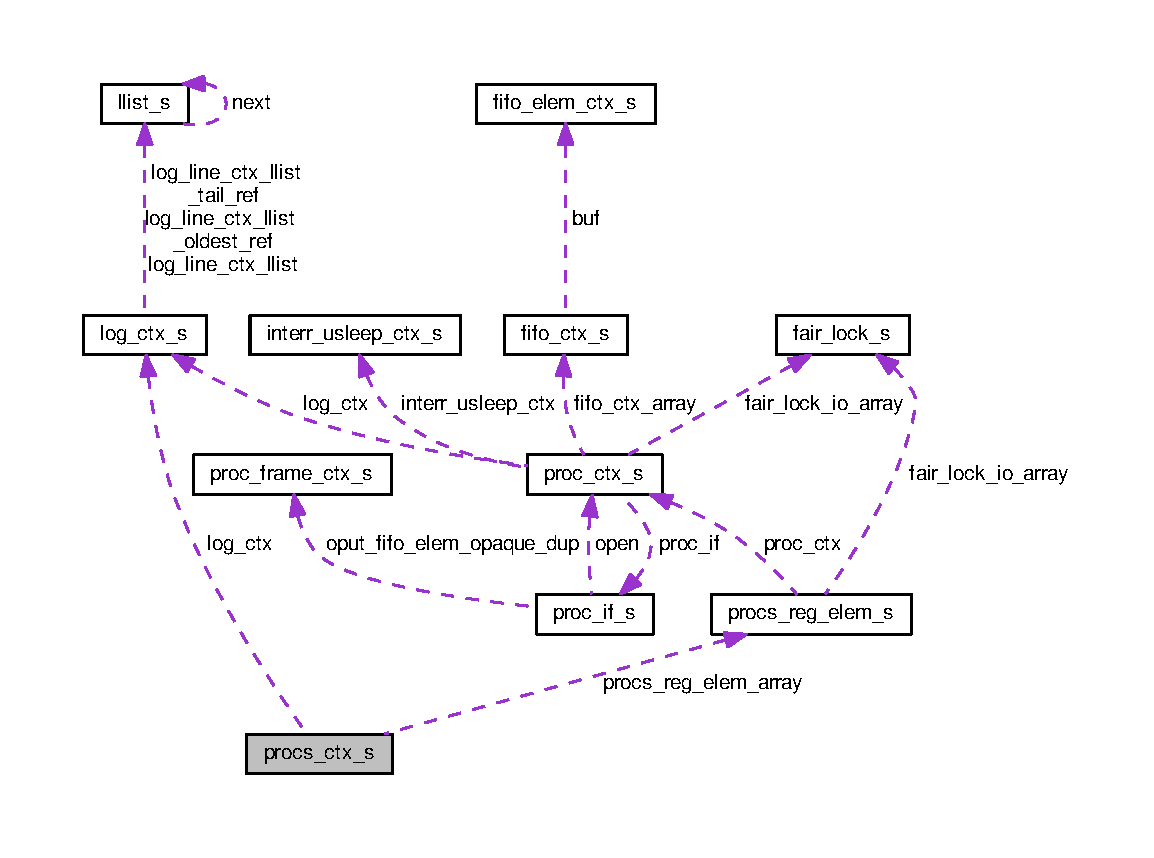
\includegraphics[width=350pt]{structprocs__ctx__s__coll__graph}
\end{center}
\end{figure}
\subsection*{Public Attributes}
\begin{DoxyCompactItemize}
\item 
char \hyperlink{structprocs__ctx__s_a00c43e06f8805e3c392802956a3c0fce}{prefix\+\_\+name} \mbox{[}256\mbox{]}
\item 
char $\ast$ \hyperlink{structprocs__ctx__s_adb507582e7611d94d41bfaafd244b99a}{procs\+\_\+href}
\item 
pthread\+\_\+mutex\+\_\+t \hyperlink{structprocs__ctx__s_a27330c986436226abfa1b5a00b7bdeb1}{api\+\_\+mutex}
\item 
\hyperlink{procs_8c_a63a78f7c86536e71715f3fcef28e11c5}{procs\+\_\+reg\+\_\+elem\+\_\+t} $\ast$ \hyperlink{structprocs__ctx__s_a9ad98a927f0a5585076b32faf26a054d}{procs\+\_\+reg\+\_\+elem\+\_\+array}
\item 
size\+\_\+t \hyperlink{structprocs__ctx__s_a083c965ff29e9b8af9215db80cca7c99}{procs\+\_\+reg\+\_\+elem\+\_\+array\+\_\+size}
\item 
\hyperlink{structlog__ctx__s}{log\+\_\+ctx\+\_\+t} $\ast$ \hyperlink{structprocs__ctx__s_ab5d529e82924052baf26478afca901fa}{log\+\_\+ctx}
\end{DoxyCompactItemize}


\subsection{Detailed Description}
Module\textquotesingle{}s instance context structure. P\+R\+O\+CS module context structure is statically defined in the program. 

Definition at line 172 of file procs.\+c.



\subsection{Member Data Documentation}
\index{procs\+\_\+ctx\+\_\+s@{procs\+\_\+ctx\+\_\+s}!api\+\_\+mutex@{api\+\_\+mutex}}
\index{api\+\_\+mutex@{api\+\_\+mutex}!procs\+\_\+ctx\+\_\+s@{procs\+\_\+ctx\+\_\+s}}
\subsubsection[{\texorpdfstring{api\+\_\+mutex}{api_mutex}}]{\setlength{\rightskip}{0pt plus 5cm}pthread\+\_\+mutex\+\_\+t procs\+\_\+ctx\+\_\+s\+::api\+\_\+mutex}\hypertarget{structprocs__ctx__s_a27330c986436226abfa1b5a00b7bdeb1}{}\label{structprocs__ctx__s_a27330c986436226abfa1b5a00b7bdeb1}
Module\textquotesingle{}s instance A\+PI mutual exclusion lock. This lock is used to provide a critical section for external applications to be able to operate concurrently and asynchronously on this module. A\+PI options are available through the function \hyperlink{procs_8c_a7af2e6f2788006cfc96ca8d811922ffa}{procs\+\_\+opt()}. \begin{DoxySeeAlso}{See also}
\hyperlink{procs_8h_a7af2e6f2788006cfc96ca8d811922ffa}{procs\+\_\+opt} 
\end{DoxySeeAlso}


Definition at line 191 of file procs.\+c.

\index{procs\+\_\+ctx\+\_\+s@{procs\+\_\+ctx\+\_\+s}!log\+\_\+ctx@{log\+\_\+ctx}}
\index{log\+\_\+ctx@{log\+\_\+ctx}!procs\+\_\+ctx\+\_\+s@{procs\+\_\+ctx\+\_\+s}}
\subsubsection[{\texorpdfstring{log\+\_\+ctx}{log_ctx}}]{\setlength{\rightskip}{0pt plus 5cm}{\bf log\+\_\+ctx\+\_\+t}$\ast$ procs\+\_\+ctx\+\_\+s\+::log\+\_\+ctx}\hypertarget{structprocs__ctx__s_ab5d529e82924052baf26478afca901fa}{}\label{structprocs__ctx__s_ab5d529e82924052baf26478afca901fa}
Externally defined L\+OG module instance context structure. 

Definition at line 210 of file procs.\+c.

\index{procs\+\_\+ctx\+\_\+s@{procs\+\_\+ctx\+\_\+s}!prefix\+\_\+name@{prefix\+\_\+name}}
\index{prefix\+\_\+name@{prefix\+\_\+name}!procs\+\_\+ctx\+\_\+s@{procs\+\_\+ctx\+\_\+s}}
\subsubsection[{\texorpdfstring{prefix\+\_\+name}{prefix_name}}]{\setlength{\rightskip}{0pt plus 5cm}char procs\+\_\+ctx\+\_\+s\+::prefix\+\_\+name\mbox{[}256\mbox{]}}\hypertarget{structprocs__ctx__s_a00c43e06f8805e3c392802956a3c0fce}{}\label{structprocs__ctx__s_a00c43e06f8805e3c392802956a3c0fce}
Module\textquotesingle{}s A\+PI R\+E\+ST prefix name (256 characters maximum). This parameter can be set by \textquotesingle{}\hyperlink{procs_8c_ac44b6ac931afbeadeb7f07b660e30bac}{procs\+\_\+open()}\textquotesingle{} function; if not (N\+U\+LL is specified), the default name \char`\"{}procs\char`\"{} is used. 

Definition at line 178 of file procs.\+c.

\index{procs\+\_\+ctx\+\_\+s@{procs\+\_\+ctx\+\_\+s}!procs\+\_\+href@{procs\+\_\+href}}
\index{procs\+\_\+href@{procs\+\_\+href}!procs\+\_\+ctx\+\_\+s@{procs\+\_\+ctx\+\_\+s}}
\subsubsection[{\texorpdfstring{procs\+\_\+href}{procs_href}}]{\setlength{\rightskip}{0pt plus 5cm}char$\ast$ procs\+\_\+ctx\+\_\+s\+::procs\+\_\+href}\hypertarget{structprocs__ctx__s_adb507582e7611d94d41bfaafd244b99a}{}\label{structprocs__ctx__s_adb507582e7611d94d41bfaafd244b99a}
Module\textquotesingle{}s A\+PI R\+E\+ST href attribute specifying the U\+RL path the A\+PI refers to. This parameter is optional (may be N\+U\+LL). 

Definition at line 183 of file procs.\+c.

\index{procs\+\_\+ctx\+\_\+s@{procs\+\_\+ctx\+\_\+s}!procs\+\_\+reg\+\_\+elem\+\_\+array@{procs\+\_\+reg\+\_\+elem\+\_\+array}}
\index{procs\+\_\+reg\+\_\+elem\+\_\+array@{procs\+\_\+reg\+\_\+elem\+\_\+array}!procs\+\_\+ctx\+\_\+s@{procs\+\_\+ctx\+\_\+s}}
\subsubsection[{\texorpdfstring{procs\+\_\+reg\+\_\+elem\+\_\+array}{procs_reg_elem_array}}]{\setlength{\rightskip}{0pt plus 5cm}{\bf procs\+\_\+reg\+\_\+elem\+\_\+t}$\ast$ procs\+\_\+ctx\+\_\+s\+::procs\+\_\+reg\+\_\+elem\+\_\+array}\hypertarget{structprocs__ctx__s_a9ad98a927f0a5585076b32faf26a054d}{}\label{structprocs__ctx__s_a9ad98a927f0a5585076b32faf26a054d}
Array listing the registered processor instances. The idea behind using an array is to have a mean to fast fetch a processor for input (receive) or output (send) operations. This array is defined with a fixed maximum size (set when calling the function \textquotesingle{}\hyperlink{procs_8c_ac44b6ac931afbeadeb7f07b660e30bac}{procs\+\_\+open()}\textquotesingle{}, but limited to a maximum of P\+R\+O\+C\+S\+\_\+\+M\+A\+X\+\_\+\+N\+U\+M\+\_\+\+P\+R\+O\+C\+\_\+\+I\+N\+S\+T\+A\+N\+C\+ES); each element of the array has a set of locks already initialized to enable concurrency. 

Definition at line 201 of file procs.\+c.

\index{procs\+\_\+ctx\+\_\+s@{procs\+\_\+ctx\+\_\+s}!procs\+\_\+reg\+\_\+elem\+\_\+array\+\_\+size@{procs\+\_\+reg\+\_\+elem\+\_\+array\+\_\+size}}
\index{procs\+\_\+reg\+\_\+elem\+\_\+array\+\_\+size@{procs\+\_\+reg\+\_\+elem\+\_\+array\+\_\+size}!procs\+\_\+ctx\+\_\+s@{procs\+\_\+ctx\+\_\+s}}
\subsubsection[{\texorpdfstring{procs\+\_\+reg\+\_\+elem\+\_\+array\+\_\+size}{procs_reg_elem_array_size}}]{\setlength{\rightskip}{0pt plus 5cm}size\+\_\+t procs\+\_\+ctx\+\_\+s\+::procs\+\_\+reg\+\_\+elem\+\_\+array\+\_\+size}\hypertarget{structprocs__ctx__s_a083c965ff29e9b8af9215db80cca7c99}{}\label{structprocs__ctx__s_a083c965ff29e9b8af9215db80cca7c99}
Size of the array of registered processors. See \textquotesingle{}\hyperlink{structprocs__ctx__s_a9ad98a927f0a5585076b32faf26a054d}{procs\+\_\+ctx\+\_\+s\+::procs\+\_\+reg\+\_\+elem\+\_\+array}\textquotesingle{} 

Definition at line 206 of file procs.\+c.



The documentation for this struct was generated from the following file\+:\begin{DoxyCompactItemize}
\item 
\hyperlink{procs_8c}{procs.\+c}\end{DoxyCompactItemize}

\hypertarget{structprocs__module__ctx__s}{}\section{procs\+\_\+module\+\_\+ctx\+\_\+s Struct Reference}
\label{structprocs__module__ctx__s}\index{procs\+\_\+module\+\_\+ctx\+\_\+s@{procs\+\_\+module\+\_\+ctx\+\_\+s}}


Collaboration diagram for procs\+\_\+module\+\_\+ctx\+\_\+s\+:\nopagebreak
\begin{figure}[H]
\begin{center}
\leavevmode
\includegraphics[width=195pt]{structprocs__module__ctx__s__coll__graph}
\end{center}
\end{figure}
\subsection*{Public Attributes}
\begin{DoxyCompactItemize}
\item 
pthread\+\_\+mutex\+\_\+t \hyperlink{structprocs__module__ctx__s_a10c3a0b462ead663af1b117abdfdadaa}{module\+\_\+api\+\_\+mutex}
\item 
\hyperlink{llist_8h_a90862badf6f9cc4e3d6348b7d60ce4f0}{llist\+\_\+t} $\ast$ \hyperlink{structprocs__module__ctx__s_a8a7a2cc3f2ee076ae11b7fdc63645f41}{proc\+\_\+if\+\_\+llist}
\end{DoxyCompactItemize}


\subsection{Detailed Description}
Module\textquotesingle{}s context structure. P\+R\+O\+CS module context structure is statically defined in the program. 

Definition at line 114 of file procs.\+c.



\subsection{Member Data Documentation}
\index{procs\+\_\+module\+\_\+ctx\+\_\+s@{procs\+\_\+module\+\_\+ctx\+\_\+s}!module\+\_\+api\+\_\+mutex@{module\+\_\+api\+\_\+mutex}}
\index{module\+\_\+api\+\_\+mutex@{module\+\_\+api\+\_\+mutex}!procs\+\_\+module\+\_\+ctx\+\_\+s@{procs\+\_\+module\+\_\+ctx\+\_\+s}}
\subsubsection[{\texorpdfstring{module\+\_\+api\+\_\+mutex}{module_api_mutex}}]{\setlength{\rightskip}{0pt plus 5cm}pthread\+\_\+mutex\+\_\+t procs\+\_\+module\+\_\+ctx\+\_\+s\+::module\+\_\+api\+\_\+mutex}\hypertarget{structprocs__module__ctx__s_a10c3a0b462ead663af1b117abdfdadaa}{}\label{structprocs__module__ctx__s_a10c3a0b462ead663af1b117abdfdadaa}
Module\textquotesingle{}s A\+PI mutual exclusion lock. This lock is used to provide a critical section for external applications to be able to operate concurrently and asynchronously on this module. A\+PI options are available through the function \hyperlink{procs_8c_a226ac6dfd7598a59b9ceab3a92239a80}{procs\+\_\+module\+\_\+opt()}. 

Definition at line 122 of file procs.\+c.

\index{procs\+\_\+module\+\_\+ctx\+\_\+s@{procs\+\_\+module\+\_\+ctx\+\_\+s}!proc\+\_\+if\+\_\+llist@{proc\+\_\+if\+\_\+llist}}
\index{proc\+\_\+if\+\_\+llist@{proc\+\_\+if\+\_\+llist}!procs\+\_\+module\+\_\+ctx\+\_\+s@{procs\+\_\+module\+\_\+ctx\+\_\+s}}
\subsubsection[{\texorpdfstring{proc\+\_\+if\+\_\+llist}{proc_if_llist}}]{\setlength{\rightskip}{0pt plus 5cm}{\bf llist\+\_\+t}$\ast$ procs\+\_\+module\+\_\+ctx\+\_\+s\+::proc\+\_\+if\+\_\+llist}\hypertarget{structprocs__module__ctx__s_a8a7a2cc3f2ee076ae11b7fdc63645f41}{}\label{structprocs__module__ctx__s_a8a7a2cc3f2ee076ae11b7fdc63645f41}
List of supported/registered processor types. Each registered processor will have a static interface (IF) entry in this linked list. \begin{DoxySeeAlso}{See also}
\hyperlink{proc__if_8h_a2b6dbff97f4d62e7a7c7674284620929}{proc\+\_\+if\+\_\+t} 
\end{DoxySeeAlso}


Definition at line 129 of file procs.\+c.



The documentation for this struct was generated from the following file\+:\begin{DoxyCompactItemize}
\item 
\hyperlink{procs_8c}{procs.\+c}\end{DoxyCompactItemize}

\hypertarget{structprocs__reg__elem__s}{}\section{procs\+\_\+reg\+\_\+elem\+\_\+s Struct Reference}
\label{structprocs__reg__elem__s}\index{procs\+\_\+reg\+\_\+elem\+\_\+s@{procs\+\_\+reg\+\_\+elem\+\_\+s}}


Collaboration diagram for procs\+\_\+reg\+\_\+elem\+\_\+s\+:\nopagebreak
\begin{figure}[H]
\begin{center}
\leavevmode
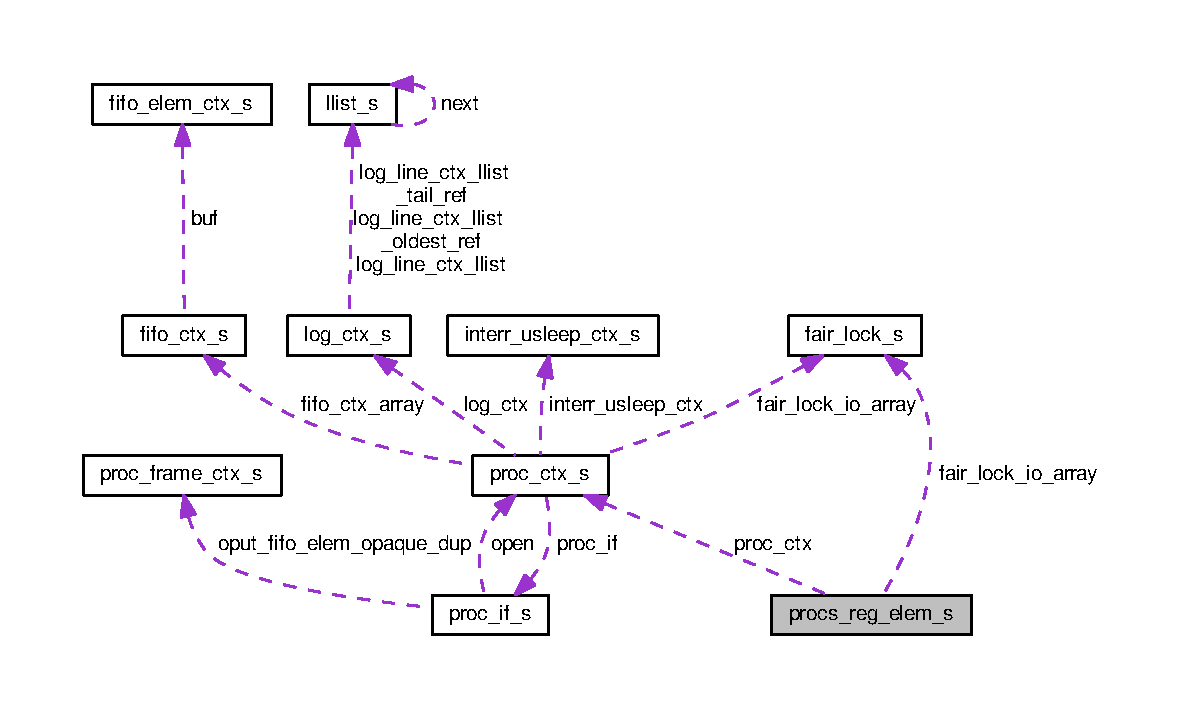
\includegraphics[width=350pt]{structprocs__reg__elem__s__coll__graph}
\end{center}
\end{figure}
\subsection*{Public Attributes}
\begin{DoxyCompactItemize}
\item 
pthread\+\_\+mutex\+\_\+t \hyperlink{structprocs__reg__elem__s_a9b7bb6d12868ba74184d95f1a2fdd2ab}{api\+\_\+mutex}
\item 
\hyperlink{structfair__lock__s}{fair\+\_\+lock\+\_\+t} $\ast$ \hyperlink{structprocs__reg__elem__s_a4de246450a9e79fe65ab600814311c6d}{fair\+\_\+lock\+\_\+io\+\_\+array} \mbox{[}P\+R\+O\+C\+\_\+\+I\+O\+\_\+\+N\+UM\mbox{]}
\item 
\hyperlink{proc_8h_ae264f89be30fc03f5053bc16d58cba05}{proc\+\_\+ctx\+\_\+t} $\ast$ \hyperlink{structprocs__reg__elem__s_aa394ff40393e8ca08c8f4c9b0c965698}{proc\+\_\+ctx}
\end{DoxyCompactItemize}


\subsection{Detailed Description}
Processors registration structure. 

Definition at line 135 of file procs.\+c.



\subsection{Member Data Documentation}
\index{procs\+\_\+reg\+\_\+elem\+\_\+s@{procs\+\_\+reg\+\_\+elem\+\_\+s}!api\+\_\+mutex@{api\+\_\+mutex}}
\index{api\+\_\+mutex@{api\+\_\+mutex}!procs\+\_\+reg\+\_\+elem\+\_\+s@{procs\+\_\+reg\+\_\+elem\+\_\+s}}
\subsubsection[{\texorpdfstring{api\+\_\+mutex}{api_mutex}}]{\setlength{\rightskip}{0pt plus 5cm}pthread\+\_\+mutex\+\_\+t procs\+\_\+reg\+\_\+elem\+\_\+s\+::api\+\_\+mutex}\hypertarget{structprocs__reg__elem__s_a9b7bb6d12868ba74184d95f1a2fdd2ab}{}\label{structprocs__reg__elem__s_a9b7bb6d12868ba74184d95f1a2fdd2ab}
Processor\textquotesingle{}s A\+PI mutual exclusion lock. This lock is used to provide a critical section for external applications to be able to use the processor\textquotesingle{}s A\+PI concurrently and asynchronously on any of the registered processor instances. Processor\textquotesingle{}s A\+PI options are available through the function \textquotesingle{}\hyperlink{proc_8c_a0367a65712bcd2e762ec1e9e3035cb3b}{proc\+\_\+opt()}\textquotesingle{} (see .\hyperlink{proc_8h}{proc.\+h}). This lock is initialized when opening this module, and is kept through the whole life of the module. 

Definition at line 146 of file procs.\+c.

\index{procs\+\_\+reg\+\_\+elem\+\_\+s@{procs\+\_\+reg\+\_\+elem\+\_\+s}!fair\+\_\+lock\+\_\+io\+\_\+array@{fair\+\_\+lock\+\_\+io\+\_\+array}}
\index{fair\+\_\+lock\+\_\+io\+\_\+array@{fair\+\_\+lock\+\_\+io\+\_\+array}!procs\+\_\+reg\+\_\+elem\+\_\+s@{procs\+\_\+reg\+\_\+elem\+\_\+s}}
\subsubsection[{\texorpdfstring{fair\+\_\+lock\+\_\+io\+\_\+array}{fair_lock_io_array}}]{\setlength{\rightskip}{0pt plus 5cm}{\bf fair\+\_\+lock\+\_\+t}$\ast$ procs\+\_\+reg\+\_\+elem\+\_\+s\+::fair\+\_\+lock\+\_\+io\+\_\+array\mbox{[}P\+R\+O\+C\+\_\+\+I\+O\+\_\+\+N\+UM\mbox{]}}\hypertarget{structprocs__reg__elem__s_a4de246450a9e79fe65ab600814311c6d}{}\label{structprocs__reg__elem__s_a4de246450a9e79fe65ab600814311c6d}
A pair of locks used to provide a critical section to execute, in mutual exclusion, the processor\textquotesingle{}s instantiating operations (register/unregister) and the input/output operations (send/receive). These locks are initialized when opening this module, and are kept through the whole life of the module. 

Definition at line 154 of file procs.\+c.

\index{procs\+\_\+reg\+\_\+elem\+\_\+s@{procs\+\_\+reg\+\_\+elem\+\_\+s}!proc\+\_\+ctx@{proc\+\_\+ctx}}
\index{proc\+\_\+ctx@{proc\+\_\+ctx}!procs\+\_\+reg\+\_\+elem\+\_\+s@{procs\+\_\+reg\+\_\+elem\+\_\+s}}
\subsubsection[{\texorpdfstring{proc\+\_\+ctx}{proc_ctx}}]{\setlength{\rightskip}{0pt plus 5cm}{\bf proc\+\_\+ctx\+\_\+t}$\ast$ procs\+\_\+reg\+\_\+elem\+\_\+s\+::proc\+\_\+ctx}\hypertarget{structprocs__reg__elem__s_aa394ff40393e8ca08c8f4c9b0c965698}{}\label{structprocs__reg__elem__s_aa394ff40393e8ca08c8f4c9b0c965698}
Processor context structure. Each instantiated processor will be registered using this pointer, in a registration array. This pointer may be N\+U\+LL in the register, meaning that an empty slot is available for registering new processors. To access a registered processor, this pointer will be fetched from the registration array. \begin{DoxySeeAlso}{See also}
\hyperlink{procs_8c_ad411ade07d8515e93bc2e7abf2b1e765}{procs\+\_\+module\+\_\+ctx\+\_\+t} 

procs\+\_\+reg\+\_\+elem\+\_\+array 
\end{DoxySeeAlso}


Definition at line 165 of file procs.\+c.



The documentation for this struct was generated from the following file\+:\begin{DoxyCompactItemize}
\item 
\hyperlink{procs_8c}{procs.\+c}\end{DoxyCompactItemize}

\input{classSimpleClientMediaSubsession}
\input{classSimpleClientSession}
\hypertarget{classSimpleFramedSource}{}\section{Simple\+Framed\+Source Class Reference}
\label{classSimpleFramedSource}\index{Simple\+Framed\+Source@{Simple\+Framed\+Source}}


Inheritance diagram for Simple\+Framed\+Source\+:\nopagebreak
\begin{figure}[H]
\begin{center}
\leavevmode
\includegraphics[width=190pt]{classSimpleFramedSource__inherit__graph}
\end{center}
\end{figure}


Collaboration diagram for Simple\+Framed\+Source\+:\nopagebreak
\begin{figure}[H]
\begin{center}
\leavevmode
\includegraphics[width=251pt]{classSimpleFramedSource__coll__graph}
\end{center}
\end{figure}
\subsection*{Public Member Functions}
\begin{DoxyCompactItemize}
\item 
void \hyperlink{classSimpleFramedSource_aeadfcbc8eeb78ada43c9c247e6a707af}{deliver\+Frame} ()
\end{DoxyCompactItemize}
\subsection*{Static Public Member Functions}
\begin{DoxyCompactItemize}
\item 
static \hyperlink{classSimpleFramedSource}{Simple\+Framed\+Source} $\ast$ {\bfseries create\+New} (Usage\+Environment \&env, \hyperlink{structlog__ctx__s}{log\+\_\+ctx\+\_\+t} $\ast$log\+\_\+ctx)\hypertarget{classSimpleFramedSource_a3c02f3f751c4298e6940b3745c9202ad}{}\label{classSimpleFramedSource_a3c02f3f751c4298e6940b3745c9202ad}

\end{DoxyCompactItemize}
\subsection*{Public Attributes}
\begin{DoxyCompactItemize}
\item 
\hyperlink{fifo_8c_acf3f21e64cbabccd8420c306740820c1}{fifo\+\_\+ctx\+\_\+t} $\ast$ \hyperlink{classSimpleFramedSource_ab93999240c393d2d3035dc7e5292eb2c}{m\+\_\+fifo\+\_\+ctx}
\item 
volatile Event\+Trigger\+Id \hyperlink{classSimpleFramedSource_a6de7be242a550522e914316487fa112e}{m\+\_\+event\+Trigger\+Id}
\end{DoxyCompactItemize}
\subsection*{Protected Member Functions}
\begin{DoxyCompactItemize}
\item 
{\bfseries Simple\+Framed\+Source} (Usage\+Environment \&, \hyperlink{structlog__ctx__s}{log\+\_\+ctx\+\_\+t} $\ast$)\hypertarget{classSimpleFramedSource_ab1d618908865999c517ad8082657da00}{}\label{classSimpleFramedSource_ab1d618908865999c517ad8082657da00}

\end{DoxyCompactItemize}


\subsection{Detailed Description}
So-\/called \char`\"{}framed-\/source\char`\"{} class prototype. 

Definition at line 324 of file live555\+\_\+rtsp.\+cpp.



\subsection{Member Function Documentation}
\index{Simple\+Framed\+Source@{Simple\+Framed\+Source}!deliver\+Frame@{deliver\+Frame}}
\index{deliver\+Frame@{deliver\+Frame}!Simple\+Framed\+Source@{Simple\+Framed\+Source}}
\subsubsection[{\texorpdfstring{deliver\+Frame()}{deliverFrame()}}]{\setlength{\rightskip}{0pt plus 5cm}void Simple\+Framed\+Source\+::deliver\+Frame (
\begin{DoxyParamCaption}
{}
\end{DoxyParamCaption}
)}\hypertarget{classSimpleFramedSource_aeadfcbc8eeb78ada43c9c247e6a707af}{}\label{classSimpleFramedSource_aeadfcbc8eeb78ada43c9c247e6a707af}
This function is called when new frame data is available from the device.

This function is called when new frame data is available from the device. We deliver this data by copying it to the \textquotesingle{}downstream\textquotesingle{} object, using the following parameters (class members)\+: $\ast$$\ast$$\ast$$\ast$ \textquotesingle{}in\textquotesingle{} parameters (these should {\itshape not} be modified by this function)\+: $\ast$$\ast$ f\+To\+: The frame data is copied to this address. (Note that the variable \char`\"{}f\+To\char`\"{} is {\itshape not} modified. Instead, the frame data is copied to the address pointed to by \char`\"{}f\+To\char`\"{}.) $\ast$$\ast$ f\+Max\+Size\+: This is the maximum number of bytes that can be copied (If the actual frame is larger than this, then it should be truncated, and \char`\"{}f\+Num\+Truncated\+Bytes\char`\"{} set accordingly.) $\ast$$\ast$$\ast$$\ast$$\ast$ \textquotesingle{}out\textquotesingle{} parameters (these are modified by this function)\+: $\ast$$\ast$ f\+Frame\+Size\+: Should be set to the delivered frame size ($<$= f\+Max\+Size). $\ast$$\ast$ f\+Num\+Truncated\+Bytes\+: Should be set iff the delivered frame would have been bigger than \char`\"{}f\+Max\+Size\char`\"{}, in which case it\textquotesingle{}s set to the number of bytes that have been omitted. $\ast$$\ast$ f\+Presentation\+Time\+: Should be set to the frame\textquotesingle{}s presentation time (seconds, microseconds). This time must be aligned with \textquotesingle{}wall-\/clock time\textquotesingle{} -\/i.\+e., the time that you would get by calling \char`\"{}gettimeofday()\char`\"{}. $\ast$$\ast$ f\+Duration\+In\+Microseconds\+: Should be set to the frame\textquotesingle{}s duration, if known. If, however, the device is a \textquotesingle{}live source\textquotesingle{} (e.\+g., encoded from a camera or microphone), then we probably don\textquotesingle{}t need to set this variable, because -\/in this case-\/ data will never arrive \textquotesingle{}early\textquotesingle{}. 

Definition at line 1879 of file live555\+\_\+rtsp.\+cpp.



\subsection{Member Data Documentation}
\index{Simple\+Framed\+Source@{Simple\+Framed\+Source}!m\+\_\+event\+Trigger\+Id@{m\+\_\+event\+Trigger\+Id}}
\index{m\+\_\+event\+Trigger\+Id@{m\+\_\+event\+Trigger\+Id}!Simple\+Framed\+Source@{Simple\+Framed\+Source}}
\subsubsection[{\texorpdfstring{m\+\_\+event\+Trigger\+Id}{m_eventTriggerId}}]{\setlength{\rightskip}{0pt plus 5cm}volatile Event\+Trigger\+Id Simple\+Framed\+Source\+::m\+\_\+event\+Trigger\+Id}\hypertarget{classSimpleFramedSource_a6de7be242a550522e914316487fa112e}{}\label{classSimpleFramedSource_a6de7be242a550522e914316487fa112e}
Unambiguous frame consuming method event trigger identifier. 

Definition at line 341 of file live555\+\_\+rtsp.\+cpp.

\index{Simple\+Framed\+Source@{Simple\+Framed\+Source}!m\+\_\+fifo\+\_\+ctx@{m\+\_\+fifo\+\_\+ctx}}
\index{m\+\_\+fifo\+\_\+ctx@{m\+\_\+fifo\+\_\+ctx}!Simple\+Framed\+Source@{Simple\+Framed\+Source}}
\subsubsection[{\texorpdfstring{m\+\_\+fifo\+\_\+ctx}{m_fifo_ctx}}]{\setlength{\rightskip}{0pt plus 5cm}{\bf fifo\+\_\+ctx\+\_\+t}$\ast$ Simple\+Framed\+Source\+::m\+\_\+fifo\+\_\+ctx}\hypertarget{classSimpleFramedSource_ab93999240c393d2d3035dc7e5292eb2c}{}\label{classSimpleFramedSource_ab93999240c393d2d3035dc7e5292eb2c}
Input frames F\+I\+FO buffer. 

Definition at line 337 of file live555\+\_\+rtsp.\+cpp.



The documentation for this class was generated from the following file\+:\begin{DoxyCompactItemize}
\item 
\hyperlink{live555__rtsp_8cpp}{live555\+\_\+rtsp.\+cpp}\end{DoxyCompactItemize}

\input{classSimpleMediaSubsession}
\input{classSimpleRTPSink2}
\hypertarget{classSimpleRTSPClient}{}\section{Simple\+R\+T\+S\+P\+Client Class Reference}
\label{classSimpleRTSPClient}\index{Simple\+R\+T\+S\+P\+Client@{Simple\+R\+T\+S\+P\+Client}}


Inheritance diagram for Simple\+R\+T\+S\+P\+Client\+:\nopagebreak
\begin{figure}[H]
\begin{center}
\leavevmode
\includegraphics[width=179pt]{classSimpleRTSPClient__inherit__graph}
\end{center}
\end{figure}


Collaboration diagram for Simple\+R\+T\+S\+P\+Client\+:\nopagebreak
\begin{figure}[H]
\begin{center}
\leavevmode
\includegraphics[width=350pt]{classSimpleRTSPClient__coll__graph}
\end{center}
\end{figure}
\subsection*{Static Public Member Functions}
\begin{DoxyCompactItemize}
\item 
static \hyperlink{classSimpleRTSPClient}{Simple\+R\+T\+S\+P\+Client} $\ast$ {\bfseries create\+New} (Usage\+Environment \&env, char const $\ast$rtsp\+U\+RL, volatile int $\ast$ref\+\_\+flag\+\_\+exit, \hyperlink{fifo_8c_acf3f21e64cbabccd8420c306740820c1}{fifo\+\_\+ctx\+\_\+t} $\ast$fifo\+\_\+ctx, int verbosity\+Level=0, char const $\ast$application\+Name=N\+U\+LL, port\+Num\+Bits tunnel\+Over\+H\+T\+T\+P\+Port\+Num=0, \hyperlink{structlog__ctx__s}{log\+\_\+ctx\+\_\+t} $\ast$log\+\_\+ctx=N\+U\+LL)\hypertarget{classSimpleRTSPClient_a8568e983f40d2992964ca3875b79b643}{}\label{classSimpleRTSPClient_a8568e983f40d2992964ca3875b79b643}

\end{DoxyCompactItemize}
\subsection*{Public Attributes}
\begin{DoxyCompactItemize}
\item 
\hyperlink{classStreamClientState}{Stream\+Client\+State} {\bfseries stream\+Client\+State}\hypertarget{classSimpleRTSPClient_a44482bf42e2aec10d383fed5d9e2d128}{}\label{classSimpleRTSPClient_a44482bf42e2aec10d383fed5d9e2d128}

\item 
volatile int $\ast$ {\bfseries m\+\_\+ref\+\_\+flag\+\_\+exit}\hypertarget{classSimpleRTSPClient_a40c26da532ddbc1d36c60688fc3cb35c}{}\label{classSimpleRTSPClient_a40c26da532ddbc1d36c60688fc3cb35c}

\item 
\hyperlink{structlog__ctx__s}{log\+\_\+ctx\+\_\+t} $\ast$ {\bfseries m\+\_\+log\+\_\+ctx}\hypertarget{classSimpleRTSPClient_afb0a7189511a5433a152136a3ec90cc7}{}\label{classSimpleRTSPClient_afb0a7189511a5433a152136a3ec90cc7}

\item 
\hyperlink{fifo_8c_acf3f21e64cbabccd8420c306740820c1}{fifo\+\_\+ctx\+\_\+t} $\ast$ {\bfseries m\+\_\+fifo\+\_\+ctx}\hypertarget{classSimpleRTSPClient_abc2f811a9accfb7c6f50f3a240f33d09}{}\label{classSimpleRTSPClient_abc2f811a9accfb7c6f50f3a240f33d09}

\end{DoxyCompactItemize}
\subsection*{Protected Member Functions}
\begin{DoxyCompactItemize}
\item 
{\bfseries Simple\+R\+T\+S\+P\+Client} (Usage\+Environment \&env, char const $\ast$rtsp\+U\+RL, volatile int $\ast$ref\+\_\+flag\+\_\+exit, \hyperlink{fifo_8c_acf3f21e64cbabccd8420c306740820c1}{fifo\+\_\+ctx\+\_\+t} $\ast$fifo\+\_\+ctx, int verbosity\+Level, char const $\ast$application\+Name, port\+Num\+Bits tunnel\+Over\+H\+T\+T\+P\+Port\+Num, \hyperlink{structlog__ctx__s}{log\+\_\+ctx\+\_\+t} $\ast$log\+\_\+ctx=N\+U\+LL)\hypertarget{classSimpleRTSPClient_acc028f7094149456d884b347f720b663}{}\label{classSimpleRTSPClient_acc028f7094149456d884b347f720b663}

\end{DoxyCompactItemize}


\subsection{Detailed Description}
This class inherits R\+T\+S\+P\+Client with the objective of adding a \hyperlink{classStreamClientState}{Stream\+Client\+State} as a member for each stream, as other private variables. 

Definition at line 480 of file live555\+\_\+rtsp.\+cpp.



The documentation for this class was generated from the following file\+:\begin{DoxyCompactItemize}
\item 
\hyperlink{live555__rtsp_8cpp}{live555\+\_\+rtsp.\+cpp}\end{DoxyCompactItemize}

\input{structstat__codes__lu__ctx__s}
\input{classStreamClientState}
\input{structthr__ctx__s}
\input{structvideo__settings__dec__ctx__s}
\input{structvideo__settings__enc__ctx__s}
\chapter{File Documentation}
\input{audio__settings_8c}
\input{audio__settings_8h}
\hypertarget{bitparser_8c}{}\section{bitparser.\+c File Reference}
\label{bitparser_8c}\index{bitparser.\+c@{bitparser.\+c}}
{\ttfamily \#include \char`\"{}bitparser.\+h\char`\"{}}\\*
{\ttfamily \#include $<$stdlib.\+h$>$}\\*
{\ttfamily \#include $<$string.\+h$>$}\\*
{\ttfamily \#include $<$stdint.\+h$>$}\\*
{\ttfamily \#include $<$endian.\+h$>$}\\*
{\ttfamily \#include \char`\"{}log.\+h\char`\"{}}\\*
{\ttfamily \#include \char`\"{}stat\+\_\+codes.\+h\char`\"{}}\\*
{\ttfamily \#include \char`\"{}check\+\_\+utils.\+h\char`\"{}}\\*
Include dependency graph for bitparser.\+c\+:\nopagebreak
\begin{figure}[H]
\begin{center}
\leavevmode
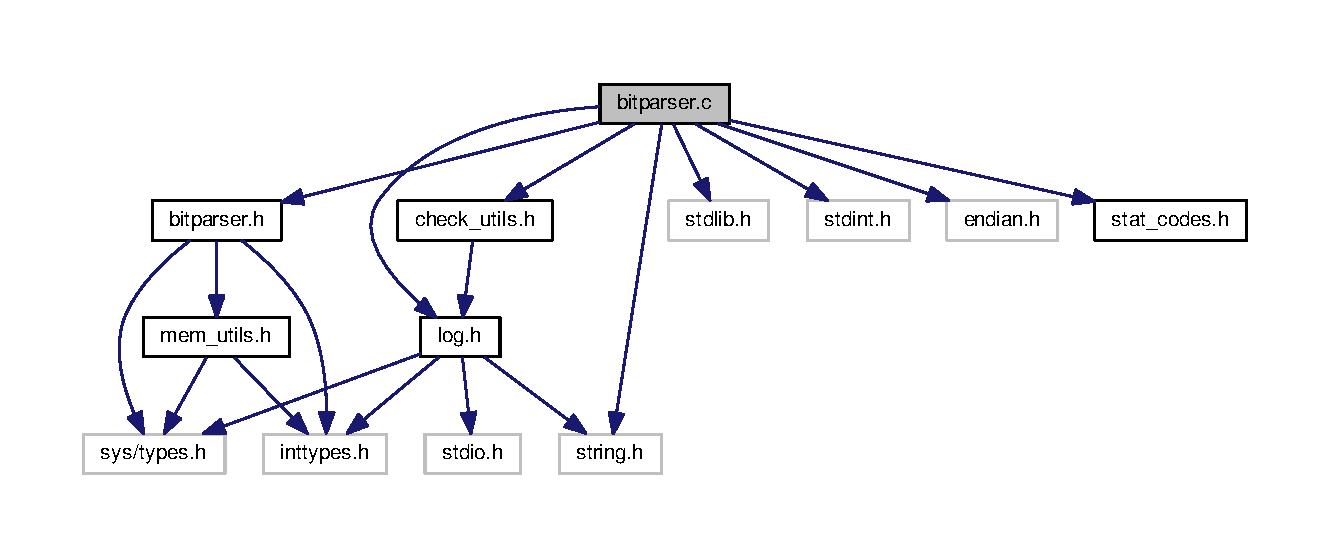
\includegraphics[width=350pt]{bitparser_8c__incl}
\end{center}
\end{figure}
\subsection*{Macros}
\begin{DoxyCompactItemize}
\item 
\#define {\bfseries L\+OG}(...)\hypertarget{bitparser_8c_a3577749fb48d57a158b8ac1a0b3ab57e}{}\label{bitparser_8c_a3577749fb48d57a158b8ac1a0b3ab57e}

\item 
\#define {\bfseries S\+HL}(x,  y)~( ((x) $<$$<$ (y)) )\hypertarget{bitparser_8c_a80eab7d0e8f0448b76dd9f531383091c}{}\label{bitparser_8c_a80eab7d0e8f0448b76dd9f531383091c}

\item 
\#define {\bfseries S\+HR}(x,  y)~( ((y) \& D\+P\+A\+T\+HW) ? 0 \+: ((x) $>$$>$ (y)) )\hypertarget{bitparser_8c_a44b9891b1dfe126cee07835e15379e5e}{}\label{bitparser_8c_a44b9891b1dfe126cee07835e15379e5e}

\item 
\#define {\bfseries G\+L\+B\+I\+C\+\_\+\+E\+N\+D\+I\+AN}\hypertarget{bitparser_8c_aae7be4c29a9a93d88877ee8aa1b6711f}{}\label{bitparser_8c_aae7be4c29a9a93d88877ee8aa1b6711f}

\item 
\#define {\bfseries S\+W\+A\+P2}(x)~be16toh(x)\hypertarget{bitparser_8c_af43b8a3b1b980b36b07ded4e3f4f322d}{}\label{bitparser_8c_af43b8a3b1b980b36b07ded4e3f4f322d}

\item 
\#define {\bfseries S\+W\+A\+P4}(x)~be32toh(x)\hypertarget{bitparser_8c_aa8de42bd4c7b9bec58163c664aa29e28}{}\label{bitparser_8c_aa8de42bd4c7b9bec58163c664aa29e28}

\item 
\#define {\bfseries S\+W\+A\+P8}(x)~be64toh(x)\hypertarget{bitparser_8c_a5229d89ff2d909df696cbe04830bb62a}{}\label{bitparser_8c_a5229d89ff2d909df696cbe04830bb62a}

\item 
\#define {\bfseries I\+S\+\_\+\+P\+O\+W\+\_\+\+O\+F\+\_\+2}(x)
\end{DoxyCompactItemize}
\subsection*{Functions}
\begin{DoxyCompactItemize}
\item 
\hyperlink{structbitparser__ctx__s}{bitparser\+\_\+ctx\+\_\+t} $\ast$ \hyperlink{bitparser_8c_af26ccd7d3d277e8954f62897894d4d39}{bitparser\+\_\+open} (void $\ast$buf, size\+\_\+t buf\+\_\+size)
\item 
void \hyperlink{bitparser_8c_ab50b395e7d30cff122fbbe148b3004b9}{bitparser\+\_\+close} (\hyperlink{structbitparser__ctx__s}{bitparser\+\_\+ctx\+\_\+t} $\ast$$\ast$ref\+\_\+bitparser\+\_\+ctx)
\item 
void \hyperlink{bitparser_8c_ac61c1322cb8aab746f8618b29341d133}{bitparser\+\_\+flush} (\hyperlink{structbitparser__ctx__s}{bitparser\+\_\+ctx\+\_\+t} $\ast$bitparser\+\_\+ctx, size\+\_\+t n)
\item 
W\+O\+R\+D\+\_\+T \hyperlink{bitparser_8c_a844fac9f2863568e995dacaf42b14673}{bitparser\+\_\+get} (\hyperlink{structbitparser__ctx__s}{bitparser\+\_\+ctx\+\_\+t} $\ast$bitparser\+\_\+ctx, size\+\_\+t n)
\item 
W\+O\+R\+D\+\_\+T \hyperlink{bitparser_8c_a24545011cfb691796f436ea716ca3e56}{bitparser\+\_\+show} (\hyperlink{structbitparser__ctx__s}{bitparser\+\_\+ctx\+\_\+t} $\ast$bitparser\+\_\+ctx, size\+\_\+t n)
\item 
void $\ast$ \hyperlink{bitparser_8c_afbf0a52141277133963b46a7b3ffbe83}{bitparser\+\_\+copy\+\_\+bytes} (\hyperlink{structbitparser__ctx__s}{bitparser\+\_\+ctx\+\_\+t} $\ast$bitparser\+\_\+ctx, size\+\_\+t cnt)
\item 
void \hyperlink{bitparser_8c_aab7a3581adfca72d040447b208366cff}{bitparser\+\_\+align\+\_\+2byte} (\hyperlink{structbitparser__ctx__s}{bitparser\+\_\+ctx\+\_\+t} $\ast$bitparser\+\_\+ctx)
\end{DoxyCompactItemize}


\subsection{Detailed Description}
\begin{DoxyAuthor}{Author}
Rafael Antoniello 
\end{DoxyAuthor}


\subsection{Macro Definition Documentation}
\index{bitparser.\+c@{bitparser.\+c}!I\+S\+\_\+\+P\+O\+W\+\_\+\+O\+F\+\_\+2@{I\+S\+\_\+\+P\+O\+W\+\_\+\+O\+F\+\_\+2}}
\index{I\+S\+\_\+\+P\+O\+W\+\_\+\+O\+F\+\_\+2@{I\+S\+\_\+\+P\+O\+W\+\_\+\+O\+F\+\_\+2}!bitparser.\+c@{bitparser.\+c}}
\subsubsection[{\texorpdfstring{I\+S\+\_\+\+P\+O\+W\+\_\+\+O\+F\+\_\+2}{IS_POW_OF_2}}]{\setlength{\rightskip}{0pt plus 5cm}\#define I\+S\+\_\+\+P\+O\+W\+\_\+\+O\+F\+\_\+2(
\begin{DoxyParamCaption}
\item[{}]{x}
\end{DoxyParamCaption}
)}\hypertarget{bitparser_8c_ab103a0aa2d1cc3000e0e7833362d8813}{}\label{bitparser_8c_ab103a0aa2d1cc3000e0e7833362d8813}
{\bfseries Value\+:}
\begin{DoxyCode}
(\(\backslash\)
        ((x)!= 0)&& (((x)& ((x)- 1))== 0)\(\backslash\)
        )
\end{DoxyCode}


Definition at line 76 of file bitparser.\+c.



\subsection{Function Documentation}
\index{bitparser.\+c@{bitparser.\+c}!bitparser\+\_\+align\+\_\+2byte@{bitparser\+\_\+align\+\_\+2byte}}
\index{bitparser\+\_\+align\+\_\+2byte@{bitparser\+\_\+align\+\_\+2byte}!bitparser.\+c@{bitparser.\+c}}
\subsubsection[{\texorpdfstring{bitparser\+\_\+align\+\_\+2byte(bitparser\+\_\+ctx\+\_\+t $\ast$bitparser\+\_\+ctx)}{bitparser_align_2byte(bitparser_ctx_t *bitparser_ctx)}}]{\setlength{\rightskip}{0pt plus 5cm}void bitparser\+\_\+align\+\_\+2byte (
\begin{DoxyParamCaption}
\item[{{\bf bitparser\+\_\+ctx\+\_\+t} $\ast$}]{bitparser\+\_\+ctx}
\end{DoxyParamCaption}
)}\hypertarget{bitparser_8c_aab7a3581adfca72d040447b208366cff}{}\label{bitparser_8c_aab7a3581adfca72d040447b208366cff}
Align bit parser to the next byte boundary 
\begin{DoxyParams}{Parameters}
{\em bitparser\+\_\+ctx} & Pointer to bit-\/parser context structure. \\
\hline
\end{DoxyParams}


Definition at line 217 of file bitparser.\+c.

\index{bitparser.\+c@{bitparser.\+c}!bitparser\+\_\+close@{bitparser\+\_\+close}}
\index{bitparser\+\_\+close@{bitparser\+\_\+close}!bitparser.\+c@{bitparser.\+c}}
\subsubsection[{\texorpdfstring{bitparser\+\_\+close(bitparser\+\_\+ctx\+\_\+t $\ast$$\ast$ref\+\_\+bitparser\+\_\+ctx)}{bitparser_close(bitparser_ctx_t **ref_bitparser_ctx)}}]{\setlength{\rightskip}{0pt plus 5cm}void bitparser\+\_\+close (
\begin{DoxyParamCaption}
\item[{{\bf bitparser\+\_\+ctx\+\_\+t} $\ast$$\ast$}]{ref\+\_\+bitparser\+\_\+ctx}
\end{DoxyParamCaption}
)}\hypertarget{bitparser_8c_ab50b395e7d30cff122fbbe148b3004b9}{}\label{bitparser_8c_ab50b395e7d30cff122fbbe148b3004b9}
// F\+I\+X\+M\+E!! 

Definition at line 115 of file bitparser.\+c.

\index{bitparser.\+c@{bitparser.\+c}!bitparser\+\_\+copy\+\_\+bytes@{bitparser\+\_\+copy\+\_\+bytes}}
\index{bitparser\+\_\+copy\+\_\+bytes@{bitparser\+\_\+copy\+\_\+bytes}!bitparser.\+c@{bitparser.\+c}}
\subsubsection[{\texorpdfstring{bitparser\+\_\+copy\+\_\+bytes(bitparser\+\_\+ctx\+\_\+t $\ast$bitparser\+\_\+ctx, size\+\_\+t cnt)}{bitparser_copy_bytes(bitparser_ctx_t *bitparser_ctx, size_t cnt)}}]{\setlength{\rightskip}{0pt plus 5cm}void$\ast$ bitparser\+\_\+copy\+\_\+bytes (
\begin{DoxyParamCaption}
\item[{{\bf bitparser\+\_\+ctx\+\_\+t} $\ast$}]{bitparser\+\_\+ctx, }
\item[{size\+\_\+t}]{cnt}
\end{DoxyParamCaption}
)}\hypertarget{bitparser_8c_afbf0a52141277133963b46a7b3ffbe83}{}\label{bitparser_8c_afbf0a52141277133963b46a7b3ffbe83}
Copy \textquotesingle{}cnt\textquotesingle{} bytes from bit-\/parser internal buffer to a dynamically (heap) allocated memory. Important\+: note that this function requires copy operation to be byte aligned; thus, this function copies the byte block corresponding to the current value of the internal bit-\/counter. 
\begin{DoxyParams}{Parameters}
{\em bitparser\+\_\+ctx} & Pointer to bit-\/parser context structure \\
\hline
{\em cnt} & Number of bytes to copy \\
\hline
\end{DoxyParams}
\begin{DoxyReturn}{Returns}
Pointer to the copy allocation. The allocation should be freed later by the caller. 
\end{DoxyReturn}


Definition at line 186 of file bitparser.\+c.

\index{bitparser.\+c@{bitparser.\+c}!bitparser\+\_\+flush@{bitparser\+\_\+flush}}
\index{bitparser\+\_\+flush@{bitparser\+\_\+flush}!bitparser.\+c@{bitparser.\+c}}
\subsubsection[{\texorpdfstring{bitparser\+\_\+flush(bitparser\+\_\+ctx\+\_\+t $\ast$bitparser\+\_\+ctx, size\+\_\+t n)}{bitparser_flush(bitparser_ctx_t *bitparser_ctx, size_t n)}}]{\setlength{\rightskip}{0pt plus 5cm}void bitparser\+\_\+flush (
\begin{DoxyParamCaption}
\item[{{\bf bitparser\+\_\+ctx\+\_\+t} $\ast$}]{bitparser\+\_\+ctx, }
\item[{size\+\_\+t}]{n}
\end{DoxyParamCaption}
)}\hypertarget{bitparser_8c_ac61c1322cb8aab746f8618b29341d133}{}\label{bitparser_8c_ac61c1322cb8aab746f8618b29341d133}
Flush next n bits out of buffer (Advance internal bit-\/counter by \textquotesingle{}n\textquotesingle{} bits). 
\begin{DoxyParams}{Parameters}
{\em bitparser\+\_\+ctx} & Pointer to bit-\/parser context structure \\
\hline
{\em n} & number of bits to flush. \\
\hline
\end{DoxyParams}


Definition at line 129 of file bitparser.\+c.

\index{bitparser.\+c@{bitparser.\+c}!bitparser\+\_\+get@{bitparser\+\_\+get}}
\index{bitparser\+\_\+get@{bitparser\+\_\+get}!bitparser.\+c@{bitparser.\+c}}
\subsubsection[{\texorpdfstring{bitparser\+\_\+get(bitparser\+\_\+ctx\+\_\+t $\ast$bitparser\+\_\+ctx, size\+\_\+t n)}{bitparser_get(bitparser_ctx_t *bitparser_ctx, size_t n)}}]{\setlength{\rightskip}{0pt plus 5cm}W\+O\+R\+D\+\_\+T bitparser\+\_\+get (
\begin{DoxyParamCaption}
\item[{{\bf bitparser\+\_\+ctx\+\_\+t} $\ast$}]{bitparser\+\_\+ctx, }
\item[{size\+\_\+t}]{n}
\end{DoxyParamCaption}
)}\hypertarget{bitparser_8c_a844fac9f2863568e995dacaf42b14673}{}\label{bitparser_8c_a844fac9f2863568e995dacaf42b14673}
Get next n bits right aligned in an unsigned 32/64-\/bit word. Bits are \char`\"{}flushed\char`\"{} from internal buffer, incrementing internal bit counter. 
\begin{DoxyParams}{Parameters}
{\em bitparser\+\_\+ctx} & Pointer to bit-\/parser context structure \\
\hline
{\em n} & Number of bits to get (internal bit counter is incremented by \textquotesingle{}n\textquotesingle{}) \\
\hline
\end{DoxyParams}
\begin{DoxyReturn}{Returns}
Unsigned 32/64-\/bit word showing next n bits right aligned (stream bits are ordered from left to right). 
\end{DoxyReturn}


Definition at line 163 of file bitparser.\+c.

\index{bitparser.\+c@{bitparser.\+c}!bitparser\+\_\+open@{bitparser\+\_\+open}}
\index{bitparser\+\_\+open@{bitparser\+\_\+open}!bitparser.\+c@{bitparser.\+c}}
\subsubsection[{\texorpdfstring{bitparser\+\_\+open(void $\ast$buf, size\+\_\+t buf\+\_\+size)}{bitparser_open(void *buf, size_t buf_size)}}]{\setlength{\rightskip}{0pt plus 5cm}{\bf bitparser\+\_\+ctx\+\_\+t}$\ast$ bitparser\+\_\+open (
\begin{DoxyParamCaption}
\item[{void $\ast$}]{buf, }
\item[{size\+\_\+t}]{buf\+\_\+size}
\end{DoxyParamCaption}
)}\hypertarget{bitparser_8c_af26ccd7d3d277e8954f62897894d4d39}{}\label{bitparser_8c_af26ccd7d3d277e8954f62897894d4d39}
//\+F\+I\+X\+M\+E!! Initializes the bit-\/parser context attributes, getting ready for parsing. 
\begin{DoxyParams}{Parameters}
{\em bitparser\+\_\+ctx} & Pointer to bit-\/parser context structure \\
\hline
{\em buf} & Pointer to buffer to be parsed. \\
\hline
{\em buf\+\_\+size} & Parsing buffer size in bytes. Value M\+U\+ST be a multiple of 8. \\
\hline
\end{DoxyParams}
\begin{DoxyReturn}{Returns}
Status code (refer to \textquotesingle{}stat\+\_\+codes\+\_\+ctx\+\_\+t\textquotesingle{} type). 
\end{DoxyReturn}
\begin{DoxySeeAlso}{See also}
stat\+\_\+codes\+\_\+ctx\+\_\+t 
\end{DoxySeeAlso}


Definition at line 82 of file bitparser.\+c.

\index{bitparser.\+c@{bitparser.\+c}!bitparser\+\_\+show@{bitparser\+\_\+show}}
\index{bitparser\+\_\+show@{bitparser\+\_\+show}!bitparser.\+c@{bitparser.\+c}}
\subsubsection[{\texorpdfstring{bitparser\+\_\+show(bitparser\+\_\+ctx\+\_\+t $\ast$bitparser\+\_\+ctx, size\+\_\+t n)}{bitparser_show(bitparser_ctx_t *bitparser_ctx, size_t n)}}]{\setlength{\rightskip}{0pt plus 5cm}W\+O\+R\+D\+\_\+T bitparser\+\_\+show (
\begin{DoxyParamCaption}
\item[{{\bf bitparser\+\_\+ctx\+\_\+t} $\ast$}]{bitparser\+\_\+ctx, }
\item[{size\+\_\+t}]{n}
\end{DoxyParamCaption}
)}\hypertarget{bitparser_8c_a24545011cfb691796f436ea716ca3e56}{}\label{bitparser_8c_a24545011cfb691796f436ea716ca3e56}
Show next n bits right aligned in an unsigned 32/64-\/bit word. Internal buffer bit counter is not modified (namely, consecutive identical calls to this function will return the same value). 
\begin{DoxyParams}{Parameters}
{\em bitparser\+\_\+ctx} & Pointer to bit-\/parser context structure \\
\hline
{\em n} & Number of bits to show \\
\hline
\end{DoxyParams}
\begin{DoxyReturn}{Returns}
Unsigned 32/64-\/bit word showing next n bits right aligned (stream bits are ordered from left to right). 
\end{DoxyReturn}


Definition at line 175 of file bitparser.\+c.


\hypertarget{bitparser_8h}{}\section{bitparser.\+h File Reference}
\label{bitparser_8h}\index{bitparser.\+h@{bitparser.\+h}}


Bit parsing module utility.  


{\ttfamily \#include $<$sys/types.\+h$>$}\\*
{\ttfamily \#include $<$inttypes.\+h$>$}\\*
{\ttfamily \#include \char`\"{}mem\+\_\+utils.\+h\char`\"{}}\\*
Include dependency graph for bitparser.\+h\+:\nopagebreak
\begin{figure}[H]
\begin{center}
\leavevmode
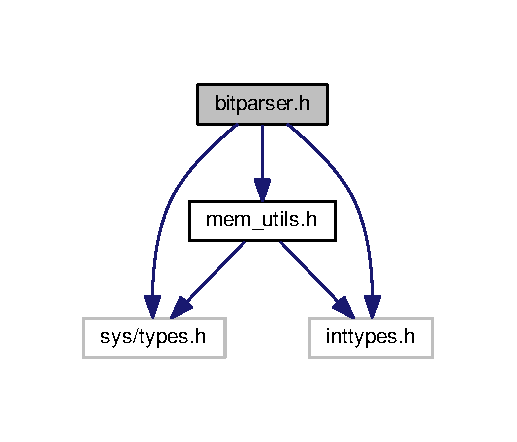
\includegraphics[width=248pt]{bitparser_8h__incl}
\end{center}
\end{figure}
This graph shows which files directly or indirectly include this file\+:\nopagebreak
\begin{figure}[H]
\begin{center}
\leavevmode
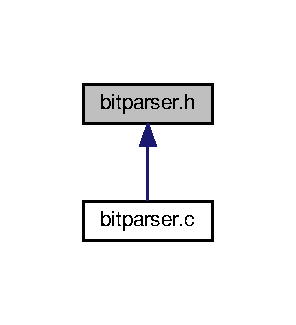
\includegraphics[width=142pt]{bitparser_8h__dep__incl}
\end{center}
\end{figure}
\subsection*{Classes}
\begin{DoxyCompactItemize}
\item 
struct \hyperlink{structbitparser__ctx__s}{bitparser\+\_\+ctx\+\_\+s}
\end{DoxyCompactItemize}
\subsection*{Macros}
\begin{DoxyCompactItemize}
\item 
\#define \hyperlink{bitparser_8h_a6211570943b20529b90b1f0c27df21c1}{L\+I\+T\+T\+L\+E\+E\+N\+D\+I\+AN}
\end{DoxyCompactItemize}
\subsection*{Typedefs}
\begin{DoxyCompactItemize}
\item 
typedef struct \hyperlink{structbitparser__ctx__s}{bitparser\+\_\+ctx\+\_\+s} {\bfseries bitparser\+\_\+ctx\+\_\+t}\hypertarget{bitparser_8h_a2e9afa7411b124d20a519bae84be53d9}{}\label{bitparser_8h_a2e9afa7411b124d20a519bae84be53d9}

\end{DoxyCompactItemize}
\subsection*{Functions}
\begin{DoxyCompactItemize}
\item 
\hyperlink{structbitparser__ctx__s}{bitparser\+\_\+ctx\+\_\+t} $\ast$ \hyperlink{bitparser_8h_af26ccd7d3d277e8954f62897894d4d39}{bitparser\+\_\+open} (void $\ast$buf, size\+\_\+t buf\+\_\+size)
\item 
void \hyperlink{bitparser_8h_ab50b395e7d30cff122fbbe148b3004b9}{bitparser\+\_\+close} (\hyperlink{structbitparser__ctx__s}{bitparser\+\_\+ctx\+\_\+t} $\ast$$\ast$ref\+\_\+bitparser\+\_\+ctx)
\item 
void \hyperlink{bitparser_8h_ac61c1322cb8aab746f8618b29341d133}{bitparser\+\_\+flush} (\hyperlink{structbitparser__ctx__s}{bitparser\+\_\+ctx\+\_\+t} $\ast$bitparser\+\_\+ctx, size\+\_\+t n)
\item 
W\+O\+R\+D\+\_\+T \hyperlink{bitparser_8h_a844fac9f2863568e995dacaf42b14673}{bitparser\+\_\+get} (\hyperlink{structbitparser__ctx__s}{bitparser\+\_\+ctx\+\_\+t} $\ast$bitparser\+\_\+ctx, size\+\_\+t n)
\item 
W\+O\+R\+D\+\_\+T \hyperlink{bitparser_8h_a24545011cfb691796f436ea716ca3e56}{bitparser\+\_\+show} (\hyperlink{structbitparser__ctx__s}{bitparser\+\_\+ctx\+\_\+t} $\ast$bitparser\+\_\+ctx, size\+\_\+t n)
\item 
void $\ast$ \hyperlink{bitparser_8h_afbf0a52141277133963b46a7b3ffbe83}{bitparser\+\_\+copy\+\_\+bytes} (\hyperlink{structbitparser__ctx__s}{bitparser\+\_\+ctx\+\_\+t} $\ast$bitparser\+\_\+ctx, size\+\_\+t cnt)
\item 
void \hyperlink{bitparser_8h_aab7a3581adfca72d040447b208366cff}{bitparser\+\_\+align\+\_\+2byte} (\hyperlink{structbitparser__ctx__s}{bitparser\+\_\+ctx\+\_\+t} $\ast$bitparser\+\_\+ctx)
\end{DoxyCompactItemize}


\subsection{Detailed Description}
Bit parsing module utility. 

\begin{DoxyAuthor}{Author}
Rafael Antoniello 
\end{DoxyAuthor}


\subsection{Macro Definition Documentation}
\index{bitparser.\+h@{bitparser.\+h}!L\+I\+T\+T\+L\+E\+E\+N\+D\+I\+AN@{L\+I\+T\+T\+L\+E\+E\+N\+D\+I\+AN}}
\index{L\+I\+T\+T\+L\+E\+E\+N\+D\+I\+AN@{L\+I\+T\+T\+L\+E\+E\+N\+D\+I\+AN}!bitparser.\+h@{bitparser.\+h}}
\subsubsection[{\texorpdfstring{L\+I\+T\+T\+L\+E\+E\+N\+D\+I\+AN}{LITTLEENDIAN}}]{\setlength{\rightskip}{0pt plus 5cm}\#define L\+I\+T\+T\+L\+E\+E\+N\+D\+I\+AN}\hypertarget{bitparser_8h_a6211570943b20529b90b1f0c27df21c1}{}\label{bitparser_8h_a6211570943b20529b90b1f0c27df21c1}
Endianess\+: define either little (un-\/comment definition below) or big endian (comment definition). 

Definition at line 49 of file bitparser.\+h.



\subsection{Function Documentation}
\index{bitparser.\+h@{bitparser.\+h}!bitparser\+\_\+align\+\_\+2byte@{bitparser\+\_\+align\+\_\+2byte}}
\index{bitparser\+\_\+align\+\_\+2byte@{bitparser\+\_\+align\+\_\+2byte}!bitparser.\+h@{bitparser.\+h}}
\subsubsection[{\texorpdfstring{bitparser\+\_\+align\+\_\+2byte(bitparser\+\_\+ctx\+\_\+t $\ast$bitparser\+\_\+ctx)}{bitparser_align_2byte(bitparser_ctx_t *bitparser_ctx)}}]{\setlength{\rightskip}{0pt plus 5cm}void bitparser\+\_\+align\+\_\+2byte (
\begin{DoxyParamCaption}
\item[{{\bf bitparser\+\_\+ctx\+\_\+t} $\ast$}]{bitparser\+\_\+ctx}
\end{DoxyParamCaption}
)}\hypertarget{bitparser_8h_aab7a3581adfca72d040447b208366cff}{}\label{bitparser_8h_aab7a3581adfca72d040447b208366cff}
Align bit parser to the next byte boundary 
\begin{DoxyParams}{Parameters}
{\em bitparser\+\_\+ctx} & Pointer to bit-\/parser context structure. \\
\hline
\end{DoxyParams}


Definition at line 217 of file bitparser.\+c.

\index{bitparser.\+h@{bitparser.\+h}!bitparser\+\_\+close@{bitparser\+\_\+close}}
\index{bitparser\+\_\+close@{bitparser\+\_\+close}!bitparser.\+h@{bitparser.\+h}}
\subsubsection[{\texorpdfstring{bitparser\+\_\+close(bitparser\+\_\+ctx\+\_\+t $\ast$$\ast$ref\+\_\+bitparser\+\_\+ctx)}{bitparser_close(bitparser_ctx_t **ref_bitparser_ctx)}}]{\setlength{\rightskip}{0pt plus 5cm}void bitparser\+\_\+close (
\begin{DoxyParamCaption}
\item[{{\bf bitparser\+\_\+ctx\+\_\+t} $\ast$$\ast$}]{ref\+\_\+bitparser\+\_\+ctx}
\end{DoxyParamCaption}
)}\hypertarget{bitparser_8h_ab50b395e7d30cff122fbbe148b3004b9}{}\label{bitparser_8h_ab50b395e7d30cff122fbbe148b3004b9}
// F\+I\+X\+M\+E!! 

Definition at line 115 of file bitparser.\+c.

\index{bitparser.\+h@{bitparser.\+h}!bitparser\+\_\+copy\+\_\+bytes@{bitparser\+\_\+copy\+\_\+bytes}}
\index{bitparser\+\_\+copy\+\_\+bytes@{bitparser\+\_\+copy\+\_\+bytes}!bitparser.\+h@{bitparser.\+h}}
\subsubsection[{\texorpdfstring{bitparser\+\_\+copy\+\_\+bytes(bitparser\+\_\+ctx\+\_\+t $\ast$bitparser\+\_\+ctx, size\+\_\+t cnt)}{bitparser_copy_bytes(bitparser_ctx_t *bitparser_ctx, size_t cnt)}}]{\setlength{\rightskip}{0pt plus 5cm}void$\ast$ bitparser\+\_\+copy\+\_\+bytes (
\begin{DoxyParamCaption}
\item[{{\bf bitparser\+\_\+ctx\+\_\+t} $\ast$}]{bitparser\+\_\+ctx, }
\item[{size\+\_\+t}]{cnt}
\end{DoxyParamCaption}
)}\hypertarget{bitparser_8h_afbf0a52141277133963b46a7b3ffbe83}{}\label{bitparser_8h_afbf0a52141277133963b46a7b3ffbe83}
Copy \textquotesingle{}cnt\textquotesingle{} bytes from bit-\/parser internal buffer to a dynamically (heap) allocated memory. Important\+: note that this function requires copy operation to be byte aligned; thus, this function copies the byte block corresponding to the current value of the internal bit-\/counter. 
\begin{DoxyParams}{Parameters}
{\em bitparser\+\_\+ctx} & Pointer to bit-\/parser context structure \\
\hline
{\em cnt} & Number of bytes to copy \\
\hline
\end{DoxyParams}
\begin{DoxyReturn}{Returns}
Pointer to the copy allocation. The allocation should be freed later by the caller. 
\end{DoxyReturn}


Definition at line 186 of file bitparser.\+c.

\index{bitparser.\+h@{bitparser.\+h}!bitparser\+\_\+flush@{bitparser\+\_\+flush}}
\index{bitparser\+\_\+flush@{bitparser\+\_\+flush}!bitparser.\+h@{bitparser.\+h}}
\subsubsection[{\texorpdfstring{bitparser\+\_\+flush(bitparser\+\_\+ctx\+\_\+t $\ast$bitparser\+\_\+ctx, size\+\_\+t n)}{bitparser_flush(bitparser_ctx_t *bitparser_ctx, size_t n)}}]{\setlength{\rightskip}{0pt plus 5cm}void bitparser\+\_\+flush (
\begin{DoxyParamCaption}
\item[{{\bf bitparser\+\_\+ctx\+\_\+t} $\ast$}]{bitparser\+\_\+ctx, }
\item[{size\+\_\+t}]{n}
\end{DoxyParamCaption}
)}\hypertarget{bitparser_8h_ac61c1322cb8aab746f8618b29341d133}{}\label{bitparser_8h_ac61c1322cb8aab746f8618b29341d133}
Flush next n bits out of buffer (Advance internal bit-\/counter by \textquotesingle{}n\textquotesingle{} bits). 
\begin{DoxyParams}{Parameters}
{\em bitparser\+\_\+ctx} & Pointer to bit-\/parser context structure \\
\hline
{\em n} & number of bits to flush. \\
\hline
\end{DoxyParams}


Definition at line 129 of file bitparser.\+c.

\index{bitparser.\+h@{bitparser.\+h}!bitparser\+\_\+get@{bitparser\+\_\+get}}
\index{bitparser\+\_\+get@{bitparser\+\_\+get}!bitparser.\+h@{bitparser.\+h}}
\subsubsection[{\texorpdfstring{bitparser\+\_\+get(bitparser\+\_\+ctx\+\_\+t $\ast$bitparser\+\_\+ctx, size\+\_\+t n)}{bitparser_get(bitparser_ctx_t *bitparser_ctx, size_t n)}}]{\setlength{\rightskip}{0pt plus 5cm}W\+O\+R\+D\+\_\+T bitparser\+\_\+get (
\begin{DoxyParamCaption}
\item[{{\bf bitparser\+\_\+ctx\+\_\+t} $\ast$}]{bitparser\+\_\+ctx, }
\item[{size\+\_\+t}]{n}
\end{DoxyParamCaption}
)}\hypertarget{bitparser_8h_a844fac9f2863568e995dacaf42b14673}{}\label{bitparser_8h_a844fac9f2863568e995dacaf42b14673}
Get next n bits right aligned in an unsigned 32/64-\/bit word. Bits are \char`\"{}flushed\char`\"{} from internal buffer, incrementing internal bit counter. 
\begin{DoxyParams}{Parameters}
{\em bitparser\+\_\+ctx} & Pointer to bit-\/parser context structure \\
\hline
{\em n} & Number of bits to get (internal bit counter is incremented by \textquotesingle{}n\textquotesingle{}) \\
\hline
\end{DoxyParams}
\begin{DoxyReturn}{Returns}
Unsigned 32/64-\/bit word showing next n bits right aligned (stream bits are ordered from left to right). 
\end{DoxyReturn}


Definition at line 163 of file bitparser.\+c.

\index{bitparser.\+h@{bitparser.\+h}!bitparser\+\_\+open@{bitparser\+\_\+open}}
\index{bitparser\+\_\+open@{bitparser\+\_\+open}!bitparser.\+h@{bitparser.\+h}}
\subsubsection[{\texorpdfstring{bitparser\+\_\+open(void $\ast$buf, size\+\_\+t buf\+\_\+size)}{bitparser_open(void *buf, size_t buf_size)}}]{\setlength{\rightskip}{0pt plus 5cm}{\bf bitparser\+\_\+ctx\+\_\+t}$\ast$ bitparser\+\_\+open (
\begin{DoxyParamCaption}
\item[{void $\ast$}]{buf, }
\item[{size\+\_\+t}]{buf\+\_\+size}
\end{DoxyParamCaption}
)}\hypertarget{bitparser_8h_af26ccd7d3d277e8954f62897894d4d39}{}\label{bitparser_8h_af26ccd7d3d277e8954f62897894d4d39}
//\+F\+I\+X\+M\+E!! Initializes the bit-\/parser context attributes, getting ready for parsing. 
\begin{DoxyParams}{Parameters}
{\em bitparser\+\_\+ctx} & Pointer to bit-\/parser context structure \\
\hline
{\em buf} & Pointer to buffer to be parsed. \\
\hline
{\em buf\+\_\+size} & Parsing buffer size in bytes. Value M\+U\+ST be a multiple of 8. \\
\hline
\end{DoxyParams}
\begin{DoxyReturn}{Returns}
Status code (refer to \textquotesingle{}stat\+\_\+codes\+\_\+ctx\+\_\+t\textquotesingle{} type). 
\end{DoxyReturn}
\begin{DoxySeeAlso}{See also}
stat\+\_\+codes\+\_\+ctx\+\_\+t 
\end{DoxySeeAlso}


Definition at line 82 of file bitparser.\+c.

\index{bitparser.\+h@{bitparser.\+h}!bitparser\+\_\+show@{bitparser\+\_\+show}}
\index{bitparser\+\_\+show@{bitparser\+\_\+show}!bitparser.\+h@{bitparser.\+h}}
\subsubsection[{\texorpdfstring{bitparser\+\_\+show(bitparser\+\_\+ctx\+\_\+t $\ast$bitparser\+\_\+ctx, size\+\_\+t n)}{bitparser_show(bitparser_ctx_t *bitparser_ctx, size_t n)}}]{\setlength{\rightskip}{0pt plus 5cm}W\+O\+R\+D\+\_\+T bitparser\+\_\+show (
\begin{DoxyParamCaption}
\item[{{\bf bitparser\+\_\+ctx\+\_\+t} $\ast$}]{bitparser\+\_\+ctx, }
\item[{size\+\_\+t}]{n}
\end{DoxyParamCaption}
)}\hypertarget{bitparser_8h_a24545011cfb691796f436ea716ca3e56}{}\label{bitparser_8h_a24545011cfb691796f436ea716ca3e56}
Show next n bits right aligned in an unsigned 32/64-\/bit word. Internal buffer bit counter is not modified (namely, consecutive identical calls to this function will return the same value). 
\begin{DoxyParams}{Parameters}
{\em bitparser\+\_\+ctx} & Pointer to bit-\/parser context structure \\
\hline
{\em n} & Number of bits to show \\
\hline
\end{DoxyParams}
\begin{DoxyReturn}{Returns}
Unsigned 32/64-\/bit word showing next n bits right aligned (stream bits are ordered from left to right). 
\end{DoxyReturn}


Definition at line 175 of file bitparser.\+c.


\hypertarget{bypass_8c}{}\section{bypass.\+c File Reference}
\label{bypass_8c}\index{bypass.\+c@{bypass.\+c}}
{\ttfamily \#include \char`\"{}bypass.\+h\char`\"{}}\\*
{\ttfamily \#include $<$stdlib.\+h$>$}\\*
{\ttfamily \#include $<$unistd.\+h$>$}\\*
{\ttfamily \#include $<$string.\+h$>$}\\*
{\ttfamily \#include $<$pthread.\+h$>$}\\*
{\ttfamily \#include $<$libcjson/c\+J\+S\+O\+N.\+h$>$}\\*
{\ttfamily \#include $<$libmediaprocsutils/log.\+h$>$}\\*
{\ttfamily \#include $<$libmediaprocsutils/stat\+\_\+codes.\+h$>$}\\*
{\ttfamily \#include $<$libmediaprocsutils/check\+\_\+utils.\+h$>$}\\*
{\ttfamily \#include $<$libmediaprocsutils/fifo.\+h$>$}\\*
{\ttfamily \#include $<$libmediaprocs/proc\+\_\+if.\+h$>$}\\*
{\ttfamily \#include $<$libmediaprocs/proc.\+h$>$}\\*
Include dependency graph for bypass.\+c\+:\nopagebreak
\begin{figure}[H]
\begin{center}
\leavevmode
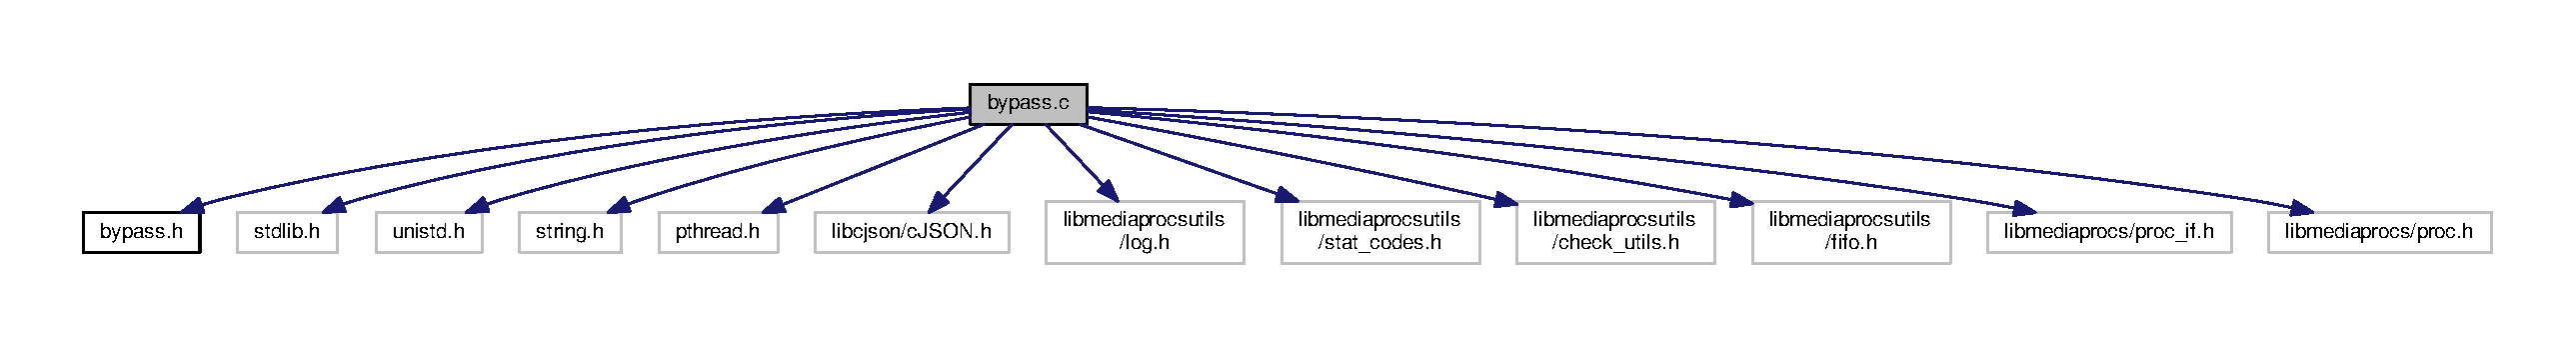
\includegraphics[width=350pt]{bypass_8c__incl}
\end{center}
\end{figure}
\subsection*{Classes}
\begin{DoxyCompactItemize}
\item 
struct \hyperlink{structbypass__settings__ctx__s}{bypass\+\_\+settings\+\_\+ctx\+\_\+s}
\item 
struct \hyperlink{structbypass__ctx__s}{bypass\+\_\+ctx\+\_\+s}
\end{DoxyCompactItemize}
\subsection*{Typedefs}
\begin{DoxyCompactItemize}
\item 
typedef struct \hyperlink{structbypass__settings__ctx__s}{bypass\+\_\+settings\+\_\+ctx\+\_\+s} \hyperlink{bypass_8c_a36f41e7b435b7b49cd23e7506e42e7c0}{bypass\+\_\+settings\+\_\+ctx\+\_\+t}
\item 
typedef struct \hyperlink{structbypass__ctx__s}{bypass\+\_\+ctx\+\_\+s} \hyperlink{bypass_8c_a9a5d0d7e68f66eaa1afed1fded1cd1c2}{bypass\+\_\+ctx\+\_\+t}
\end{DoxyCompactItemize}
\subsection*{Functions}
\begin{DoxyCompactItemize}
\item 
static \hyperlink{proc_8h_ae264f89be30fc03f5053bc16d58cba05}{proc\+\_\+ctx\+\_\+t} $\ast$ \hyperlink{bypass_8c_a13e7300dab549ef116086ba693c40bce}{bypass\+\_\+open} (const \hyperlink{proc_8h_a679816cf30e0b7a8f3e7464e67a6a844}{proc\+\_\+if\+\_\+t} $\ast$proc\+\_\+if, const char $\ast$settings\+\_\+str, \hyperlink{structlog__ctx__s}{log\+\_\+ctx\+\_\+t} $\ast$log\+\_\+ctx, va\+\_\+list arg)
\item 
static void \hyperlink{bypass_8c_a357ded261525987762d1cdde4169a873}{bypass\+\_\+close} (\hyperlink{proc_8h_ae264f89be30fc03f5053bc16d58cba05}{proc\+\_\+ctx\+\_\+t} $\ast$$\ast$ref\+\_\+proc\+\_\+ctx)
\item 
static int \hyperlink{bypass_8c_a43b4dc7aaf4b148b02818c1565707b80}{bypass\+\_\+process\+\_\+frame} (\hyperlink{proc_8h_ae264f89be30fc03f5053bc16d58cba05}{proc\+\_\+ctx\+\_\+t} $\ast$proc\+\_\+ctx, \hyperlink{fifo_8c_acf3f21e64cbabccd8420c306740820c1}{fifo\+\_\+ctx\+\_\+t} $\ast$iput\+\_\+fifo\+\_\+ctx, \hyperlink{fifo_8c_acf3f21e64cbabccd8420c306740820c1}{fifo\+\_\+ctx\+\_\+t} $\ast$oput\+\_\+fifo\+\_\+ctx)
\item 
static int \hyperlink{bypass_8c_ae15807b95ca7fb1c3f262ec5827d8f8d}{bypass\+\_\+rest\+\_\+put} (\hyperlink{proc_8h_ae264f89be30fc03f5053bc16d58cba05}{proc\+\_\+ctx\+\_\+t} $\ast$proc\+\_\+ctx, const char $\ast$str)
\item 
static int \hyperlink{bypass_8c_a02d52ff6844e3ac59b8d444086970afd}{bypass\+\_\+rest\+\_\+get} (\hyperlink{proc_8h_ae264f89be30fc03f5053bc16d58cba05}{proc\+\_\+ctx\+\_\+t} $\ast$proc\+\_\+ctx, const \hyperlink{proc__if_8h_a9bea3dae53a91f2a3e3a459d1d3e22b3}{proc\+\_\+if\+\_\+rest\+\_\+fmt\+\_\+t} rest\+\_\+fmt, void $\ast$$\ast$ref\+\_\+reponse)
\item 
static int \hyperlink{bypass_8c_ab88482b5ab6911459af79dec957e33f6}{bypass\+\_\+settings\+\_\+ctx\+\_\+init} (volatile \hyperlink{bypass_8c_a36f41e7b435b7b49cd23e7506e42e7c0}{bypass\+\_\+settings\+\_\+ctx\+\_\+t} $\ast$bypass\+\_\+settings\+\_\+ctx, \hyperlink{structlog__ctx__s}{log\+\_\+ctx\+\_\+t} $\ast$log\+\_\+ctx)
\item 
static void \hyperlink{bypass_8c_a434a20a7415b5204c0dcdd0afab196a2}{bypass\+\_\+settings\+\_\+ctx\+\_\+deinit} (volatile \hyperlink{bypass_8c_a36f41e7b435b7b49cd23e7506e42e7c0}{bypass\+\_\+settings\+\_\+ctx\+\_\+t} $\ast$bypass\+\_\+settings\+\_\+ctx, \hyperlink{structlog__ctx__s}{log\+\_\+ctx\+\_\+t} $\ast$log\+\_\+ctx)
\end{DoxyCompactItemize}
\subsection*{Variables}
\begin{DoxyCompactItemize}
\item 
const \hyperlink{proc_8h_a679816cf30e0b7a8f3e7464e67a6a844}{proc\+\_\+if\+\_\+t} \hyperlink{bypass_8c_a26ad3ea6371ce8e95085aedabc0e4a40}{proc\+\_\+if\+\_\+bypass}
\end{DoxyCompactItemize}


\subsection{Detailed Description}
\begin{DoxyAuthor}{Author}
Rafael Antoniello 
\end{DoxyAuthor}


\subsection{Typedef Documentation}
\index{bypass.\+c@{bypass.\+c}!bypass\+\_\+ctx\+\_\+t@{bypass\+\_\+ctx\+\_\+t}}
\index{bypass\+\_\+ctx\+\_\+t@{bypass\+\_\+ctx\+\_\+t}!bypass.\+c@{bypass.\+c}}
\subsubsection[{\texorpdfstring{bypass\+\_\+ctx\+\_\+t}{bypass_ctx_t}}]{\setlength{\rightskip}{0pt plus 5cm}typedef struct {\bf bypass\+\_\+ctx\+\_\+s}  {\bf bypass\+\_\+ctx\+\_\+t}}\hypertarget{bypass_8c_a9a5d0d7e68f66eaa1afed1fded1cd1c2}{}\label{bypass_8c_a9a5d0d7e68f66eaa1afed1fded1cd1c2}
Bypass processor context structure. \index{bypass.\+c@{bypass.\+c}!bypass\+\_\+settings\+\_\+ctx\+\_\+t@{bypass\+\_\+settings\+\_\+ctx\+\_\+t}}
\index{bypass\+\_\+settings\+\_\+ctx\+\_\+t@{bypass\+\_\+settings\+\_\+ctx\+\_\+t}!bypass.\+c@{bypass.\+c}}
\subsubsection[{\texorpdfstring{bypass\+\_\+settings\+\_\+ctx\+\_\+t}{bypass_settings_ctx_t}}]{\setlength{\rightskip}{0pt plus 5cm}typedef struct {\bf bypass\+\_\+settings\+\_\+ctx\+\_\+s}  {\bf bypass\+\_\+settings\+\_\+ctx\+\_\+t}}\hypertarget{bypass_8c_a36f41e7b435b7b49cd23e7506e42e7c0}{}\label{bypass_8c_a36f41e7b435b7b49cd23e7506e42e7c0}
Bypass processor settings context structure. 

\subsection{Function Documentation}
\index{bypass.\+c@{bypass.\+c}!bypass\+\_\+close@{bypass\+\_\+close}}
\index{bypass\+\_\+close@{bypass\+\_\+close}!bypass.\+c@{bypass.\+c}}
\subsubsection[{\texorpdfstring{bypass\+\_\+close(proc\+\_\+ctx\+\_\+t $\ast$$\ast$ref\+\_\+proc\+\_\+ctx)}{bypass_close(proc_ctx_t **ref_proc_ctx)}}]{\setlength{\rightskip}{0pt plus 5cm}static void bypass\+\_\+close (
\begin{DoxyParamCaption}
\item[{{\bf proc\+\_\+ctx\+\_\+t} $\ast$$\ast$}]{ref\+\_\+proc\+\_\+ctx}
\end{DoxyParamCaption}
)\hspace{0.3cm}{\ttfamily [static]}}\hypertarget{bypass_8c_a357ded261525987762d1cdde4169a873}{}\label{bypass_8c_a357ded261525987762d1cdde4169a873}
Implements the \hyperlink{structproc__if__s_af5971ac1d09d1c6ec3508c36fb286c19}{proc\+\_\+if\+\_\+s\+::close} callback. See .\hyperlink{proc__if_8h}{proc\+\_\+if.\+h} for further details. 

Definition at line 146 of file bypass.\+c.

\index{bypass.\+c@{bypass.\+c}!bypass\+\_\+open@{bypass\+\_\+open}}
\index{bypass\+\_\+open@{bypass\+\_\+open}!bypass.\+c@{bypass.\+c}}
\subsubsection[{\texorpdfstring{bypass\+\_\+open(const proc\+\_\+if\+\_\+t $\ast$proc\+\_\+if, const char $\ast$settings\+\_\+str, log\+\_\+ctx\+\_\+t $\ast$log\+\_\+ctx, va\+\_\+list arg)}{bypass_open(const proc_if_t *proc_if, const char *settings_str, log_ctx_t *log_ctx, va_list arg)}}]{\setlength{\rightskip}{0pt plus 5cm}static {\bf proc\+\_\+ctx\+\_\+t} $\ast$ bypass\+\_\+open (
\begin{DoxyParamCaption}
\item[{const {\bf proc\+\_\+if\+\_\+t} $\ast$}]{proc\+\_\+if, }
\item[{const char $\ast$}]{settings\+\_\+str, }
\item[{{\bf log\+\_\+ctx\+\_\+t} $\ast$}]{log\+\_\+ctx, }
\item[{va\+\_\+list}]{arg}
\end{DoxyParamCaption}
)\hspace{0.3cm}{\ttfamily [static]}}\hypertarget{bypass_8c_a13e7300dab549ef116086ba693c40bce}{}\label{bypass_8c_a13e7300dab549ef116086ba693c40bce}
Implements the \hyperlink{structproc__if__s_a34999576771394dfb721463c8455ba06}{proc\+\_\+if\+\_\+s\+::open} callback. See .\hyperlink{proc__if_8h}{proc\+\_\+if.\+h} for further details. 

Definition at line 107 of file bypass.\+c.

\index{bypass.\+c@{bypass.\+c}!bypass\+\_\+process\+\_\+frame@{bypass\+\_\+process\+\_\+frame}}
\index{bypass\+\_\+process\+\_\+frame@{bypass\+\_\+process\+\_\+frame}!bypass.\+c@{bypass.\+c}}
\subsubsection[{\texorpdfstring{bypass\+\_\+process\+\_\+frame(proc\+\_\+ctx\+\_\+t $\ast$proc\+\_\+ctx, fifo\+\_\+ctx\+\_\+t $\ast$iput\+\_\+fifo\+\_\+ctx, fifo\+\_\+ctx\+\_\+t $\ast$oput\+\_\+fifo\+\_\+ctx)}{bypass_process_frame(proc_ctx_t *proc_ctx, fifo_ctx_t *iput_fifo_ctx, fifo_ctx_t *oput_fifo_ctx)}}]{\setlength{\rightskip}{0pt plus 5cm}static int bypass\+\_\+process\+\_\+frame (
\begin{DoxyParamCaption}
\item[{{\bf proc\+\_\+ctx\+\_\+t} $\ast$}]{proc\+\_\+ctx, }
\item[{{\bf fifo\+\_\+ctx\+\_\+t} $\ast$}]{iput\+\_\+fifo\+\_\+ctx, }
\item[{{\bf fifo\+\_\+ctx\+\_\+t} $\ast$}]{oput\+\_\+fifo\+\_\+ctx}
\end{DoxyParamCaption}
)\hspace{0.3cm}{\ttfamily [static]}}\hypertarget{bypass_8c_a43b4dc7aaf4b148b02818c1565707b80}{}\label{bypass_8c_a43b4dc7aaf4b148b02818c1565707b80}
Implements the \hyperlink{structproc__if__s_ab67b4061f94b6f15ae40c796b6b33597}{proc\+\_\+if\+\_\+s\+::process\+\_\+frame} callback. See .\hyperlink{proc__if_8h}{proc\+\_\+if.\+h} for further details. 

Definition at line 170 of file bypass.\+c.

\index{bypass.\+c@{bypass.\+c}!bypass\+\_\+rest\+\_\+get@{bypass\+\_\+rest\+\_\+get}}
\index{bypass\+\_\+rest\+\_\+get@{bypass\+\_\+rest\+\_\+get}!bypass.\+c@{bypass.\+c}}
\subsubsection[{\texorpdfstring{bypass\+\_\+rest\+\_\+get(proc\+\_\+ctx\+\_\+t $\ast$proc\+\_\+ctx, const proc\+\_\+if\+\_\+rest\+\_\+fmt\+\_\+t rest\+\_\+fmt, void $\ast$$\ast$ref\+\_\+reponse)}{bypass_rest_get(proc_ctx_t *proc_ctx, const proc_if_rest_fmt_t rest_fmt, void **ref_reponse)}}]{\setlength{\rightskip}{0pt plus 5cm}static int bypass\+\_\+rest\+\_\+get (
\begin{DoxyParamCaption}
\item[{{\bf proc\+\_\+ctx\+\_\+t} $\ast$}]{proc\+\_\+ctx, }
\item[{const {\bf proc\+\_\+if\+\_\+rest\+\_\+fmt\+\_\+t}}]{rest\+\_\+fmt, }
\item[{void $\ast$$\ast$}]{ref\+\_\+reponse}
\end{DoxyParamCaption}
)\hspace{0.3cm}{\ttfamily [static]}}\hypertarget{bypass_8c_a02d52ff6844e3ac59b8d444086970afd}{}\label{bypass_8c_a02d52ff6844e3ac59b8d444086970afd}
Implements the \hyperlink{structproc__if__s_a1e45b33c52b931954f7a0d8a14f0db53}{proc\+\_\+if\+\_\+s\+::rest\+\_\+get} callback. See .\hyperlink{proc__if_8h}{proc\+\_\+if.\+h} for further details. 

Definition at line 241 of file bypass.\+c.

\index{bypass.\+c@{bypass.\+c}!bypass\+\_\+rest\+\_\+put@{bypass\+\_\+rest\+\_\+put}}
\index{bypass\+\_\+rest\+\_\+put@{bypass\+\_\+rest\+\_\+put}!bypass.\+c@{bypass.\+c}}
\subsubsection[{\texorpdfstring{bypass\+\_\+rest\+\_\+put(proc\+\_\+ctx\+\_\+t $\ast$proc\+\_\+ctx, const char $\ast$str)}{bypass_rest_put(proc_ctx_t *proc_ctx, const char *str)}}]{\setlength{\rightskip}{0pt plus 5cm}static int bypass\+\_\+rest\+\_\+put (
\begin{DoxyParamCaption}
\item[{{\bf proc\+\_\+ctx\+\_\+t} $\ast$}]{proc\+\_\+ctx, }
\item[{const char $\ast$}]{str}
\end{DoxyParamCaption}
)\hspace{0.3cm}{\ttfamily [static]}}\hypertarget{bypass_8c_ae15807b95ca7fb1c3f262ec5827d8f8d}{}\label{bypass_8c_ae15807b95ca7fb1c3f262ec5827d8f8d}
Implements the \hyperlink{structproc__if__s_acb4d2c240c52904ebd6904f54b1a9b78}{proc\+\_\+if\+\_\+s\+::rest\+\_\+put} callback. See .\hyperlink{proc__if_8h}{proc\+\_\+if.\+h} for further details. 

Definition at line 215 of file bypass.\+c.

\index{bypass.\+c@{bypass.\+c}!bypass\+\_\+settings\+\_\+ctx\+\_\+deinit@{bypass\+\_\+settings\+\_\+ctx\+\_\+deinit}}
\index{bypass\+\_\+settings\+\_\+ctx\+\_\+deinit@{bypass\+\_\+settings\+\_\+ctx\+\_\+deinit}!bypass.\+c@{bypass.\+c}}
\subsubsection[{\texorpdfstring{bypass\+\_\+settings\+\_\+ctx\+\_\+deinit(volatile bypass\+\_\+settings\+\_\+ctx\+\_\+t $\ast$bypass\+\_\+settings\+\_\+ctx, log\+\_\+ctx\+\_\+t $\ast$log\+\_\+ctx)}{bypass_settings_ctx_deinit(volatile bypass_settings_ctx_t *bypass_settings_ctx, log_ctx_t *log_ctx)}}]{\setlength{\rightskip}{0pt plus 5cm}static void bypass\+\_\+settings\+\_\+ctx\+\_\+deinit (
\begin{DoxyParamCaption}
\item[{volatile {\bf bypass\+\_\+settings\+\_\+ctx\+\_\+t} $\ast$}]{bypass\+\_\+settings\+\_\+ctx, }
\item[{{\bf log\+\_\+ctx\+\_\+t} $\ast$}]{log\+\_\+ctx}
\end{DoxyParamCaption}
)\hspace{0.3cm}{\ttfamily [static]}}\hypertarget{bypass_8c_a434a20a7415b5204c0dcdd0afab196a2}{}\label{bypass_8c_a434a20a7415b5204c0dcdd0afab196a2}
Release specific bypass processor settings (allocated in heap memory). 
\begin{DoxyParams}{Parameters}
{\em bypass\+\_\+settings\+\_\+ctx} & \\
\hline
{\em log\+\_\+ctx} & \\
\hline
\end{DoxyParams}


Definition at line 352 of file bypass.\+c.

\index{bypass.\+c@{bypass.\+c}!bypass\+\_\+settings\+\_\+ctx\+\_\+init@{bypass\+\_\+settings\+\_\+ctx\+\_\+init}}
\index{bypass\+\_\+settings\+\_\+ctx\+\_\+init@{bypass\+\_\+settings\+\_\+ctx\+\_\+init}!bypass.\+c@{bypass.\+c}}
\subsubsection[{\texorpdfstring{bypass\+\_\+settings\+\_\+ctx\+\_\+init(volatile bypass\+\_\+settings\+\_\+ctx\+\_\+t $\ast$bypass\+\_\+settings\+\_\+ctx, log\+\_\+ctx\+\_\+t $\ast$log\+\_\+ctx)}{bypass_settings_ctx_init(volatile bypass_settings_ctx_t *bypass_settings_ctx, log_ctx_t *log_ctx)}}]{\setlength{\rightskip}{0pt plus 5cm}static int bypass\+\_\+settings\+\_\+ctx\+\_\+init (
\begin{DoxyParamCaption}
\item[{volatile {\bf bypass\+\_\+settings\+\_\+ctx\+\_\+t} $\ast$}]{bypass\+\_\+settings\+\_\+ctx, }
\item[{{\bf log\+\_\+ctx\+\_\+t} $\ast$}]{log\+\_\+ctx}
\end{DoxyParamCaption}
)\hspace{0.3cm}{\ttfamily [static]}}\hypertarget{bypass_8c_ab88482b5ab6911459af79dec957e33f6}{}\label{bypass_8c_ab88482b5ab6911459af79dec957e33f6}
Initialize specific bypass processor settings to defaults. 
\begin{DoxyParams}{Parameters}
{\em bypass\+\_\+settings\+\_\+ctx} & \\
\hline
{\em log\+\_\+ctx} & \\
\hline
\end{DoxyParams}
\begin{DoxyReturn}{Returns}
Status code (S\+T\+A\+T\+\_\+\+S\+U\+C\+C\+E\+SS code in case of success, for other code values please refer to .\hyperlink{stat__codes_8h}{stat\+\_\+codes.\+h}). 
\end{DoxyReturn}


Definition at line 332 of file bypass.\+c.



\subsection{Variable Documentation}
\index{bypass.\+c@{bypass.\+c}!proc\+\_\+if\+\_\+bypass@{proc\+\_\+if\+\_\+bypass}}
\index{proc\+\_\+if\+\_\+bypass@{proc\+\_\+if\+\_\+bypass}!bypass.\+c@{bypass.\+c}}
\subsubsection[{\texorpdfstring{proc\+\_\+if\+\_\+bypass}{proc_if_bypass}}]{\setlength{\rightskip}{0pt plus 5cm}const {\bf proc\+\_\+if\+\_\+t} proc\+\_\+if\+\_\+bypass}\hypertarget{bypass_8c_a26ad3ea6371ce8e95085aedabc0e4a40}{}\label{bypass_8c_a26ad3ea6371ce8e95085aedabc0e4a40}
{\bfseries Initial value\+:}
\begin{DoxyCode}
=
\{
    \textcolor{stringliteral}{"bypass"}, \textcolor{stringliteral}{"bypass"}, \textcolor{stringliteral}{"video/bypass"},
    (uint64\_t)(PROC\_FEATURE\_BITRATE|PROC\_FEATURE\_REGISTER\_PTS),
    \hyperlink{bypass_8c_a13e7300dab549ef116086ba693c40bce}{bypass\_open},
    \hyperlink{bypass_8c_a357ded261525987762d1cdde4169a873}{bypass\_close},
    proc\_send\_frame\_default1,
    NULL, 
    proc\_recv\_frame\_default1,
    NULL, 
    \hyperlink{bypass_8c_ae15807b95ca7fb1c3f262ec5827d8f8d}{bypass\_rest\_put},
    \hyperlink{bypass_8c_a02d52ff6844e3ac59b8d444086970afd}{bypass\_rest\_get},
    \hyperlink{bypass_8c_a43b4dc7aaf4b148b02818c1565707b80}{bypass\_process\_frame},
    NULL, 
    (\textcolor{keywordtype}{void}*(*)(\textcolor{keyword}{const} \hyperlink{structproc__frame__ctx__s}{proc\_frame\_ctx\_t}*))\hyperlink{proc__if_8c_a778c0de8151b30abc17305131d149932}{proc\_frame\_ctx\_dup},
    (void(*)(\textcolor{keywordtype}{void}**))\hyperlink{proc__if_8c_afad6906a6da22ba369b736863c1e204e}{proc\_frame\_ctx\_release},
    (\hyperlink{structproc__frame__ctx__s}{proc\_frame\_ctx\_t}*(*)(\textcolor{keyword}{const} \textcolor{keywordtype}{void}*))proc\_frame\_ctx\_dup
\}
\end{DoxyCode}
Processor interface implementing the \char`\"{}bypass\char`\"{} processor. 

Definition at line 84 of file bypass.\+c.


\hypertarget{bypass_8h}{}\section{bypass.\+h File Reference}
\label{bypass_8h}\index{bypass.\+h@{bypass.\+h}}


\char`\"{}\+Bypass\char`\"{} or dummy processor.  


This graph shows which files directly or indirectly include this file\+:\nopagebreak
\begin{figure}[H]
\begin{center}
\leavevmode
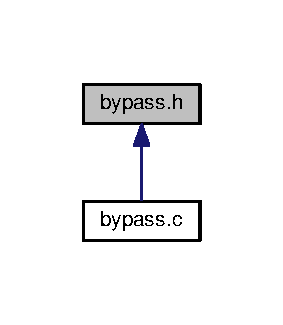
\includegraphics[width=136pt]{bypass_8h__dep__incl}
\end{center}
\end{figure}
\subsection*{Typedefs}
\begin{DoxyCompactItemize}
\item 
typedef struct \hyperlink{structproc__if__s}{proc\+\_\+if\+\_\+s} {\bfseries proc\+\_\+if\+\_\+t}\hypertarget{bypass_8h_a679816cf30e0b7a8f3e7464e67a6a844}{}\label{bypass_8h_a679816cf30e0b7a8f3e7464e67a6a844}

\end{DoxyCompactItemize}
\subsection*{Variables}
\begin{DoxyCompactItemize}
\item 
const \hyperlink{proc_8h_a679816cf30e0b7a8f3e7464e67a6a844}{proc\+\_\+if\+\_\+t} \hyperlink{bypass_8h_a26ad3ea6371ce8e95085aedabc0e4a40}{proc\+\_\+if\+\_\+bypass}
\end{DoxyCompactItemize}


\subsection{Detailed Description}
\char`\"{}\+Bypass\char`\"{} or dummy processor. 

\begin{DoxyAuthor}{Author}
Rafael Antoniello 
\end{DoxyAuthor}


\subsection{Variable Documentation}
\index{bypass.\+h@{bypass.\+h}!proc\+\_\+if\+\_\+bypass@{proc\+\_\+if\+\_\+bypass}}
\index{proc\+\_\+if\+\_\+bypass@{proc\+\_\+if\+\_\+bypass}!bypass.\+h@{bypass.\+h}}
\subsubsection[{\texorpdfstring{proc\+\_\+if\+\_\+bypass}{proc_if_bypass}}]{\setlength{\rightskip}{0pt plus 5cm}const {\bf proc\+\_\+if\+\_\+t} proc\+\_\+if\+\_\+bypass}\hypertarget{bypass_8h_a26ad3ea6371ce8e95085aedabc0e4a40}{}\label{bypass_8h_a26ad3ea6371ce8e95085aedabc0e4a40}
Processor interface implementing the \char`\"{}bypass\char`\"{} processor. 

Definition at line 84 of file bypass.\+c.


\input{check__utils_8h}
\input{codecs__muxers__loopback_8c}
\hypertarget{comm_8c}{}\section{comm.\+c File Reference}
\label{comm_8c}\index{comm.\+c@{comm.\+c}}
{\ttfamily \#include \char`\"{}comm.\+h\char`\"{}}\\*
{\ttfamily \#include $<$stdio.\+h$>$}\\*
{\ttfamily \#include $<$stdlib.\+h$>$}\\*
{\ttfamily \#include $<$unistd.\+h$>$}\\*
{\ttfamily \#include $<$stdarg.\+h$>$}\\*
{\ttfamily \#include $<$string.\+h$>$}\\*
{\ttfamily \#include $<$errno.\+h$>$}\\*
{\ttfamily \#include $<$ctype.\+h$>$}\\*
{\ttfamily \#include \char`\"{}log.\+h\char`\"{}}\\*
{\ttfamily \#include \char`\"{}stat\+\_\+codes.\+h\char`\"{}}\\*
{\ttfamily \#include \char`\"{}check\+\_\+utils.\+h\char`\"{}}\\*
{\ttfamily \#include \char`\"{}llist.\+h\char`\"{}}\\*
{\ttfamily \#include \char`\"{}uri\+\_\+parser.\+h\char`\"{}}\\*
Include dependency graph for comm.\+c\+:\nopagebreak
\begin{figure}[H]
\begin{center}
\leavevmode
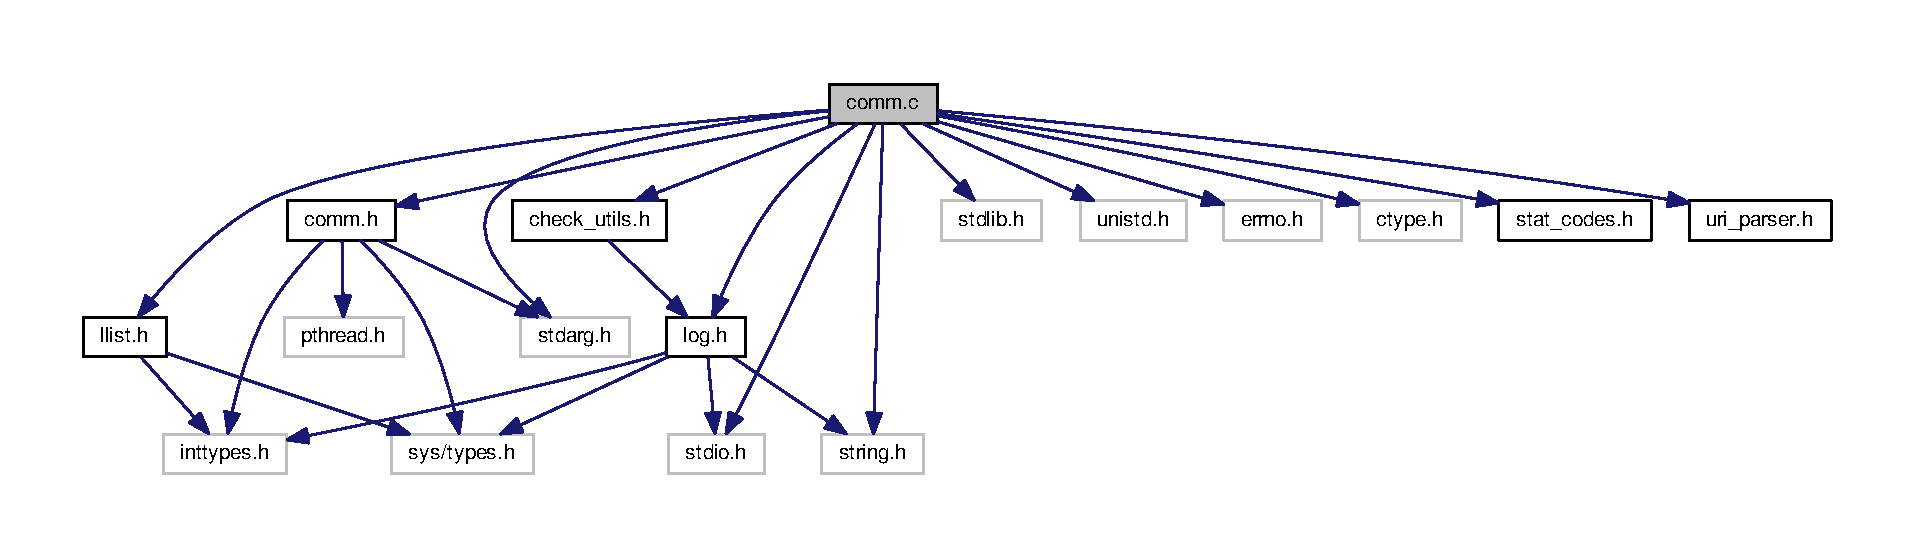
\includegraphics[width=350pt]{comm_8c__incl}
\end{center}
\end{figure}
\subsection*{Classes}
\begin{DoxyCompactItemize}
\item 
struct \hyperlink{structcomm__module__ctx__s}{comm\+\_\+module\+\_\+ctx\+\_\+s}
\end{DoxyCompactItemize}
\subsection*{Macros}
\begin{DoxyCompactItemize}
\item 
\#define \hyperlink{comm_8c_a914faae84f39085695352bd45c0fca62}{T\+A\+G\+\_\+\+IS}(T\+AG)~(strcmp(tag, T\+AG)== 0)
\end{DoxyCompactItemize}
\subsection*{Typedefs}
\begin{DoxyCompactItemize}
\item 
typedef struct \hyperlink{structcomm__module__ctx__s}{comm\+\_\+module\+\_\+ctx\+\_\+s} \hyperlink{comm_8c_abc3d2a47ed9132f55cd4eb04eea887ca}{comm\+\_\+module\+\_\+ctx\+\_\+t}
\end{DoxyCompactItemize}
\subsection*{Functions}
\begin{DoxyCompactItemize}
\item 
static int {\bfseries register\+\_\+comm\+\_\+if} (const \hyperlink{comm_8h_a0d96b9368107e517ea8253837384faf5}{comm\+\_\+if\+\_\+t} $\ast$comm\+\_\+if, \hyperlink{structlog__ctx__s}{log\+\_\+ctx\+\_\+t} $\ast$log\+\_\+ctx)\hypertarget{comm_8c_afe16ef1909e95cf2453c79586192059e}{}\label{comm_8c_afe16ef1909e95cf2453c79586192059e}

\item 
static int {\bfseries unregister\+\_\+comm\+\_\+if} (const char $\ast$scheme, \hyperlink{structlog__ctx__s}{log\+\_\+ctx\+\_\+t} $\ast$log\+\_\+ctx)\hypertarget{comm_8c_aa07542f1ac62b837ba6826eb32e8aa86}{}\label{comm_8c_aa07542f1ac62b837ba6826eb32e8aa86}

\item 
static const \hyperlink{comm_8h_a0d96b9368107e517ea8253837384faf5}{comm\+\_\+if\+\_\+t} $\ast$ {\bfseries get\+\_\+comm\+\_\+if\+\_\+by\+\_\+scheme} (const char $\ast$scheme, \hyperlink{structlog__ctx__s}{log\+\_\+ctx\+\_\+t} $\ast$log\+\_\+ctx)\hypertarget{comm_8c_a51f1531d55a566c3a257a090fdb8661b}{}\label{comm_8c_a51f1531d55a566c3a257a090fdb8661b}

\item 
static \hyperlink{comm_8h_a0d96b9368107e517ea8253837384faf5}{comm\+\_\+if\+\_\+t} $\ast$ {\bfseries comm\+\_\+if\+\_\+allocate} ()\hypertarget{comm_8c_ab7ed47b0d519325f019e749283f5a77b}{}\label{comm_8c_ab7ed47b0d519325f019e749283f5a77b}

\item 
static \hyperlink{comm_8h_a0d96b9368107e517ea8253837384faf5}{comm\+\_\+if\+\_\+t} $\ast$ {\bfseries comm\+\_\+if\+\_\+dup} (const \hyperlink{comm_8h_a0d96b9368107e517ea8253837384faf5}{comm\+\_\+if\+\_\+t} $\ast$comm\+\_\+if\+\_\+arg)\hypertarget{comm_8c_aff6d47fc99c839f92323326442418b26}{}\label{comm_8c_aff6d47fc99c839f92323326442418b26}

\item 
static void {\bfseries comm\+\_\+if\+\_\+release} (\hyperlink{comm_8h_a0d96b9368107e517ea8253837384faf5}{comm\+\_\+if\+\_\+t} $\ast$$\ast$ref\+\_\+comm\+\_\+if)\hypertarget{comm_8c_a927db50c5290cd490859963386f1db55}{}\label{comm_8c_a927db50c5290cd490859963386f1db55}

\item 
static int {\bfseries comm\+\_\+module\+\_\+url\+\_\+probe} (const char $\ast$url)\hypertarget{comm_8c_a7252feeae2a2320007aaab89f3f0f1a0}{}\label{comm_8c_a7252feeae2a2320007aaab89f3f0f1a0}

\item 
int \hyperlink{comm_8c_a80ab733009abbbe6feec774dff3485b3}{comm\+\_\+module\+\_\+open} (\hyperlink{structlog__ctx__s}{log\+\_\+ctx\+\_\+t} $\ast$log\+\_\+ctx)
\item 
void \hyperlink{comm_8c_ae7235878eac99238a0c19ac7e0672413}{comm\+\_\+module\+\_\+close} ()
\item 
int \hyperlink{comm_8c_a21edd1aa9b38d7eadecb70b5f963f437}{comm\+\_\+module\+\_\+opt} (const char $\ast$tag,...)
\item 
\hyperlink{comm_8h_aacc0873718a86d8ef4658bad2500d091}{comm\+\_\+ctx\+\_\+t} $\ast$ {\bfseries comm\+\_\+open} (const char $\ast$url, const char $\ast$local\+\_\+url, \hyperlink{comm_8h_a2604d892f8ab29dfc96bd68e2cc3086f}{comm\+\_\+mode\+\_\+t} comm\+\_\+mode, \hyperlink{structlog__ctx__s}{log\+\_\+ctx\+\_\+t} $\ast$log\+\_\+ctx,...)\hypertarget{comm_8c_a1b4ee842a6dbaefc66a776808aa331ca}{}\label{comm_8c_a1b4ee842a6dbaefc66a776808aa331ca}

\item 
void {\bfseries comm\+\_\+close} (\hyperlink{comm_8h_aacc0873718a86d8ef4658bad2500d091}{comm\+\_\+ctx\+\_\+t} $\ast$$\ast$ref\+\_\+comm\+\_\+ctx)\hypertarget{comm_8c_a9215f79ed7599d103cd2a8b9be4835d1}{}\label{comm_8c_a9215f79ed7599d103cd2a8b9be4835d1}

\item 
int {\bfseries comm\+\_\+send} (\hyperlink{comm_8h_aacc0873718a86d8ef4658bad2500d091}{comm\+\_\+ctx\+\_\+t} $\ast$comm\+\_\+ctx, const void $\ast$buf, size\+\_\+t count, struct timeval $\ast$timeout)\hypertarget{comm_8c_a4d493ddf6a804a2e03be3a5cf8980af0}{}\label{comm_8c_a4d493ddf6a804a2e03be3a5cf8980af0}

\item 
int {\bfseries comm\+\_\+recv} (\hyperlink{comm_8h_aacc0873718a86d8ef4658bad2500d091}{comm\+\_\+ctx\+\_\+t} $\ast$comm\+\_\+ctx, void $\ast$$\ast$ref\+\_\+buf, size\+\_\+t $\ast$ref\+\_\+count, char $\ast$$\ast$ref\+\_\+from, struct timeval $\ast$timeout)\hypertarget{comm_8c_afe57fe056dcf3c4f4966d0ee404c4985}{}\label{comm_8c_afe57fe056dcf3c4f4966d0ee404c4985}

\item 
int {\bfseries comm\+\_\+unblock} (\hyperlink{comm_8h_aacc0873718a86d8ef4658bad2500d091}{comm\+\_\+ctx\+\_\+t} $\ast$comm\+\_\+ctx)\hypertarget{comm_8c_a0a472f3879b3e2ea6f9575775d4a7191}{}\label{comm_8c_a0a472f3879b3e2ea6f9575775d4a7191}

\item 
int {\bfseries comm\+\_\+open\+\_\+external} (pthread\+\_\+mutex\+\_\+t $\ast$comm\+\_\+ctx\+\_\+mutex\+\_\+external, const char $\ast$url, const char $\ast$local\+\_\+url, \hyperlink{comm_8h_a2604d892f8ab29dfc96bd68e2cc3086f}{comm\+\_\+mode\+\_\+t} comm\+\_\+mode, \hyperlink{structlog__ctx__s}{log\+\_\+ctx\+\_\+t} $\ast$log\+\_\+ctx, \hyperlink{comm_8h_aacc0873718a86d8ef4658bad2500d091}{comm\+\_\+ctx\+\_\+t} $\ast$$\ast$ref\+\_\+comm\+\_\+ctx,...)\hypertarget{comm_8c_a67e1b0e92ba8fff6319e179bd80364f7}{}\label{comm_8c_a67e1b0e92ba8fff6319e179bd80364f7}

\item 
void {\bfseries comm\+\_\+close\+\_\+external} (pthread\+\_\+mutex\+\_\+t $\ast$comm\+\_\+ctx\+\_\+mutex\+\_\+external, \hyperlink{comm_8h_aacc0873718a86d8ef4658bad2500d091}{comm\+\_\+ctx\+\_\+t} $\ast$$\ast$ref\+\_\+comm\+\_\+ctx, \hyperlink{structlog__ctx__s}{log\+\_\+ctx\+\_\+t} $\ast$log\+\_\+ctx)\hypertarget{comm_8c_a2309f8c1635f6b334f2b22982ae80627}{}\label{comm_8c_a2309f8c1635f6b334f2b22982ae80627}

\item 
int {\bfseries comm\+\_\+reset\+\_\+external} (pthread\+\_\+mutex\+\_\+t $\ast$comm\+\_\+ctx\+\_\+mutex\+\_\+external, const char $\ast$new\+\_\+url, const char $\ast$local\+\_\+url, \hyperlink{comm_8h_a2604d892f8ab29dfc96bd68e2cc3086f}{comm\+\_\+mode\+\_\+t} comm\+\_\+mode, \hyperlink{structlog__ctx__s}{log\+\_\+ctx\+\_\+t} $\ast$log\+\_\+ctx, \hyperlink{comm_8h_aacc0873718a86d8ef4658bad2500d091}{comm\+\_\+ctx\+\_\+t} $\ast$$\ast$ref\+\_\+comm\+\_\+ctx\+\_\+curr,...)\hypertarget{comm_8c_a09186e043867c111cc9acbc5307e3173}{}\label{comm_8c_a09186e043867c111cc9acbc5307e3173}

\item 
int {\bfseries comm\+\_\+recv\+\_\+external} (pthread\+\_\+mutex\+\_\+t $\ast$comm\+\_\+ctx\+\_\+mutex\+\_\+external, \hyperlink{comm_8h_aacc0873718a86d8ef4658bad2500d091}{comm\+\_\+ctx\+\_\+t} $\ast$$\ast$ref\+\_\+comm\+\_\+ctx, void $\ast$$\ast$ref\+\_\+buf, size\+\_\+t $\ast$ref\+\_\+count, char $\ast$$\ast$ref\+\_\+from, struct timeval $\ast$timeout, \hyperlink{structlog__ctx__s}{log\+\_\+ctx\+\_\+t} $\ast$log\+\_\+ctx)\hypertarget{comm_8c_a8e0f63e9aba94ec4dbd092bdbc35716c}{}\label{comm_8c_a8e0f63e9aba94ec4dbd092bdbc35716c}

\end{DoxyCompactItemize}
\subsection*{Variables}
\begin{DoxyCompactItemize}
\item 
static \hyperlink{comm_8c_abc3d2a47ed9132f55cd4eb04eea887ca}{comm\+\_\+module\+\_\+ctx\+\_\+t} $\ast$ \hyperlink{comm_8c_a6652e587b89a4c651dc23cd378c1d626}{comm\+\_\+module\+\_\+ctx} = N\+U\+LL
\end{DoxyCompactItemize}


\subsection{Detailed Description}
\begin{DoxyAuthor}{Author}
Rafael Antoniello 
\end{DoxyAuthor}


\subsection{Macro Definition Documentation}
\index{comm.\+c@{comm.\+c}!T\+A\+G\+\_\+\+IS@{T\+A\+G\+\_\+\+IS}}
\index{T\+A\+G\+\_\+\+IS@{T\+A\+G\+\_\+\+IS}!comm.\+c@{comm.\+c}}
\subsubsection[{\texorpdfstring{T\+A\+G\+\_\+\+IS}{TAG_IS}}]{\setlength{\rightskip}{0pt plus 5cm}\#define T\+A\+G\+\_\+\+IS(
\begin{DoxyParamCaption}
\item[{}]{T\+AG}
\end{DoxyParamCaption}
)~(strcmp(tag, T\+AG)== 0)}\hypertarget{comm_8c_a914faae84f39085695352bd45c0fca62}{}\label{comm_8c_a914faae84f39085695352bd45c0fca62}
Returns non-\/zero if \textquotesingle{}tag\textquotesingle{} string is equal to given T\+AG string. 

Definition at line 56 of file comm.\+c.



\subsection{Typedef Documentation}
\index{comm.\+c@{comm.\+c}!comm\+\_\+module\+\_\+ctx\+\_\+t@{comm\+\_\+module\+\_\+ctx\+\_\+t}}
\index{comm\+\_\+module\+\_\+ctx\+\_\+t@{comm\+\_\+module\+\_\+ctx\+\_\+t}!comm.\+c@{comm.\+c}}
\subsubsection[{\texorpdfstring{comm\+\_\+module\+\_\+ctx\+\_\+t}{comm_module_ctx_t}}]{\setlength{\rightskip}{0pt plus 5cm}typedef struct {\bf comm\+\_\+module\+\_\+ctx\+\_\+s}  {\bf comm\+\_\+module\+\_\+ctx\+\_\+t}}\hypertarget{comm_8c_abc3d2a47ed9132f55cd4eb04eea887ca}{}\label{comm_8c_abc3d2a47ed9132f55cd4eb04eea887ca}
Module\textquotesingle{}s context structure. This structure is statically defined in the program. 

\subsection{Function Documentation}
\index{comm.\+c@{comm.\+c}!comm\+\_\+module\+\_\+close@{comm\+\_\+module\+\_\+close}}
\index{comm\+\_\+module\+\_\+close@{comm\+\_\+module\+\_\+close}!comm.\+c@{comm.\+c}}
\subsubsection[{\texorpdfstring{comm\+\_\+module\+\_\+close()}{comm_module_close()}}]{\setlength{\rightskip}{0pt plus 5cm}void comm\+\_\+module\+\_\+close (
\begin{DoxyParamCaption}
{}
\end{DoxyParamCaption}
)}\hypertarget{comm_8c_ae7235878eac99238a0c19ac7e0672413}{}\label{comm_8c_ae7235878eac99238a0c19ac7e0672413}
Close communication module. This is a global function and should be called only once at the end of the life of the application. 

Definition at line 129 of file comm.\+c.

\index{comm.\+c@{comm.\+c}!comm\+\_\+module\+\_\+open@{comm\+\_\+module\+\_\+open}}
\index{comm\+\_\+module\+\_\+open@{comm\+\_\+module\+\_\+open}!comm.\+c@{comm.\+c}}
\subsubsection[{\texorpdfstring{comm\+\_\+module\+\_\+open(log\+\_\+ctx\+\_\+t $\ast$log\+\_\+ctx)}{comm_module_open(log_ctx_t *log_ctx)}}]{\setlength{\rightskip}{0pt plus 5cm}int comm\+\_\+module\+\_\+open (
\begin{DoxyParamCaption}
\item[{{\bf log\+\_\+ctx\+\_\+t} $\ast$}]{log\+\_\+ctx}
\end{DoxyParamCaption}
)}\hypertarget{comm_8c_a80ab733009abbbe6feec774dff3485b3}{}\label{comm_8c_a80ab733009abbbe6feec774dff3485b3}
Open communication module. This is a global function and should be called only once at the very beginning and during the life of the application. 
\begin{DoxyParams}{Parameters}
{\em log\+\_\+ctx} & Pointer to a externally defined L\+OG module context structure. \\
\hline
\end{DoxyParams}
\begin{DoxyReturn}{Returns}
Status code (S\+T\+A\+T\+\_\+\+S\+U\+C\+C\+E\+SS code in case of success, for other code values please refer to .\hyperlink{stat__codes_8h}{stat\+\_\+codes.\+h}). 
\end{DoxyReturn}


Definition at line 101 of file comm.\+c.

\index{comm.\+c@{comm.\+c}!comm\+\_\+module\+\_\+opt@{comm\+\_\+module\+\_\+opt}}
\index{comm\+\_\+module\+\_\+opt@{comm\+\_\+module\+\_\+opt}!comm.\+c@{comm.\+c}}
\subsubsection[{\texorpdfstring{comm\+\_\+module\+\_\+opt(const char $\ast$tag,...)}{comm_module_opt(const char *tag,...)}}]{\setlength{\rightskip}{0pt plus 5cm}int comm\+\_\+module\+\_\+opt (
\begin{DoxyParamCaption}
\item[{const char $\ast$}]{tag, }
\item[{}]{...}
\end{DoxyParamCaption}
)}\hypertarget{comm_8c_a21edd1aa9b38d7eadecb70b5f963f437}{}\label{comm_8c_a21edd1aa9b38d7eadecb70b5f963f437}
Communication module options. This function represents the A\+PI of the communication module. This function is thread-\/safe and can be called concurrently.


\begin{DoxyParams}{Parameters}
{\em tag} & Option tag, namely, option identifier string. The following options are available\+:
\begin{DoxyEnumerate}
\item \char`\"{}\+C\+O\+M\+M\+\_\+\+R\+E\+G\+I\+S\+T\+E\+R\+\_\+\+P\+R\+O\+T\+O\char`\"{}
\item \char`\"{}\+C\+O\+M\+M\+\_\+\+U\+N\+R\+E\+G\+I\+S\+T\+E\+R\+\_\+\+P\+R\+O\+T\+O\char`\"{}
\end{DoxyEnumerate}\\
\hline
{\em ...} & Variable list of parameters according to selected option. Refer to {\bfseries Tags description} below to see the different additional parameters corresponding to each option tag. \\
\hline
\end{DoxyParams}
\begin{DoxyReturn}{Returns}
Status code (S\+T\+A\+T\+\_\+\+S\+U\+C\+C\+E\+SS code in case of success, for other code values please refer to .\hyperlink{stat__codes_8h}{stat\+\_\+codes.\+h}).
\end{DoxyReturn}
\paragraph*{Tags description (additional variable arguments per tag)}


\begin{DoxyItemize}
\item {\bfseries Tag \char`\"{}\+C\+O\+M\+M\+\_\+\+R\+E\+G\+I\+S\+T\+E\+R\+\_\+\+P\+R\+O\+T\+O\char`\"{}\+:}~\newline
 Register the interface of an specific communication protocol.~\newline
 Additional variable arguments for function \hyperlink{comm_8h_a21edd1aa9b38d7eadecb70b5f963f437}{comm\+\_\+module\+\_\+opt()} are\+:~\newline
 
\begin{DoxyParams}{Parameters}
{\em comm\+\_\+if} & Pointer to the protocol interface structure (static and unambiguous interface implementation of the type \textquotesingle{}comm\+\_\+if\+\_\+t\textquotesingle{}). Code example\+: 
\begin{DoxyCode}
1 ...
2 const comm\_if\_t comm\_if\_udp= \{
3     "udp",
4     comm\_udp\_open,
5     comm\_udp\_close,
6     comm\_udp\_send,
7     comm\_udp\_recv,
8     comm\_udp\_unblock
9 \};
10 ...
11 ret\_code= comm\_module\_opt("COMM\_REGISTER\_PROTO", &comm\_if\_udp);
\end{DoxyCode}
\\
\hline
\end{DoxyParams}

\item {\bfseries Tag \char`\"{}\+C\+O\+M\+M\+\_\+\+U\+N\+R\+E\+G\+I\+S\+T\+E\+R\+\_\+\+P\+R\+O\+T\+O\char`\"{}\+:}~\newline
 Unregister the interface of an specific communication protocol.~\newline
 Additional variable arguments for function \hyperlink{comm_8h_a21edd1aa9b38d7eadecb70b5f963f437}{comm\+\_\+module\+\_\+opt()} are\+:~\newline
 
\begin{DoxyParams}{Parameters}
{\em scheme} & Pointer to a character string with the unambiguous protocol scheme name (for example\+: \char`\"{}udp\char`\"{}, \char`\"{}file\char`\"{}, ...). Code example\+: 
\begin{DoxyCode}
1 ret\_code= comm\_module\_opt("COMM\_UNREGISTER\_PROTO", "udp");
\end{DoxyCode}
 \\
\hline
\end{DoxyParams}

\end{DoxyItemize}

Definition at line 150 of file comm.\+c.



\subsection{Variable Documentation}
\index{comm.\+c@{comm.\+c}!comm\+\_\+module\+\_\+ctx@{comm\+\_\+module\+\_\+ctx}}
\index{comm\+\_\+module\+\_\+ctx@{comm\+\_\+module\+\_\+ctx}!comm.\+c@{comm.\+c}}
\subsubsection[{\texorpdfstring{comm\+\_\+module\+\_\+ctx}{comm_module_ctx}}]{\setlength{\rightskip}{0pt plus 5cm}{\bf comm\+\_\+module\+\_\+ctx\+\_\+t}$\ast$ comm\+\_\+module\+\_\+ctx = N\+U\+LL\hspace{0.3cm}{\ttfamily [static]}}\hypertarget{comm_8c_a6652e587b89a4c651dc23cd378c1d626}{}\label{comm_8c_a6652e587b89a4c651dc23cd378c1d626}
Communication module static instance. 

Definition at line 99 of file comm.\+c.


\hypertarget{comm_8h}{}\section{comm.\+h File Reference}
\label{comm_8h}\index{comm.\+h@{comm.\+h}}


Generic communication module.  


{\ttfamily \#include $<$sys/types.\+h$>$}\\*
{\ttfamily \#include $<$inttypes.\+h$>$}\\*
{\ttfamily \#include $<$pthread.\+h$>$}\\*
{\ttfamily \#include $<$stdarg.\+h$>$}\\*
Include dependency graph for comm.\+h\+:\nopagebreak
\begin{figure}[H]
\begin{center}
\leavevmode
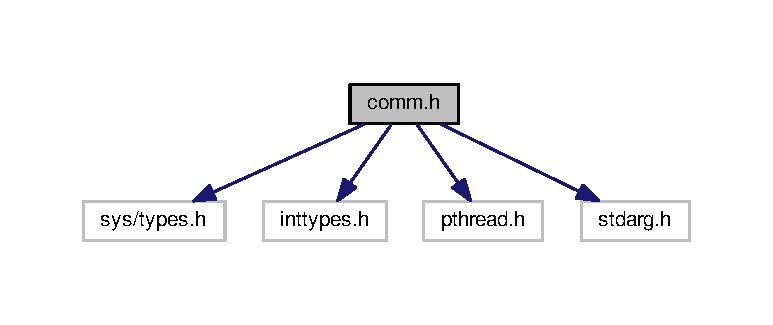
\includegraphics[width=350pt]{comm_8h__incl}
\end{center}
\end{figure}
This graph shows which files directly or indirectly include this file\+:\nopagebreak
\begin{figure}[H]
\begin{center}
\leavevmode
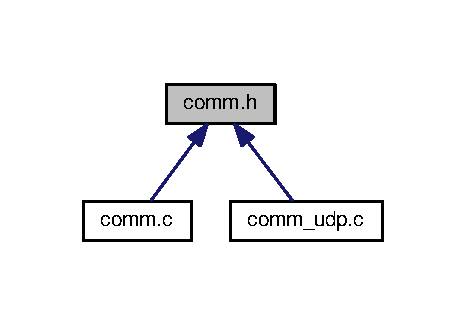
\includegraphics[width=224pt]{comm_8h__dep__incl}
\end{center}
\end{figure}
\subsection*{Classes}
\begin{DoxyCompactItemize}
\item 
struct \hyperlink{structcomm__if__s}{comm\+\_\+if\+\_\+s}
\item 
struct \hyperlink{structcomm__ctx__s}{comm\+\_\+ctx\+\_\+s}
\end{DoxyCompactItemize}
\subsection*{Typedefs}
\begin{DoxyCompactItemize}
\item 
typedef struct \hyperlink{structlog__ctx__s}{log\+\_\+ctx\+\_\+s} {\bfseries log\+\_\+ctx\+\_\+t}\hypertarget{comm_8h_a01e036219a22bb5933ddbc277cee8776}{}\label{comm_8h_a01e036219a22bb5933ddbc277cee8776}

\item 
typedef struct \hyperlink{structcomm__ctx__s}{comm\+\_\+ctx\+\_\+s} \hyperlink{comm_8h_aacc0873718a86d8ef4658bad2500d091}{comm\+\_\+ctx\+\_\+t}
\item 
typedef enum \hyperlink{comm_8h_a1d692d7421c4351b2aaf92b823bb7e29}{comm\+\_\+mode\+\_\+enum} \hyperlink{comm_8h_a2604d892f8ab29dfc96bd68e2cc3086f}{comm\+\_\+mode\+\_\+t}
\item 
typedef struct \hyperlink{structcomm__if__s}{comm\+\_\+if\+\_\+s} \hyperlink{comm_8h_a0d96b9368107e517ea8253837384faf5}{comm\+\_\+if\+\_\+t}
\end{DoxyCompactItemize}
\subsection*{Enumerations}
\begin{DoxyCompactItemize}
\item 
enum \hyperlink{comm_8h_a1d692d7421c4351b2aaf92b823bb7e29}{comm\+\_\+mode\+\_\+enum} \{ {\bfseries C\+O\+M\+M\+\_\+\+M\+O\+D\+E\+\_\+\+I\+P\+UT} = 0, 
{\bfseries C\+O\+M\+M\+\_\+\+M\+O\+D\+E\+\_\+\+O\+P\+UT}, 
{\bfseries C\+O\+M\+M\+\_\+\+M\+O\+D\+E\+\_\+\+M\+AX}
 \}
\end{DoxyCompactItemize}
\subsection*{Functions}
\begin{DoxyCompactItemize}
\item 
int \hyperlink{comm_8h_a80ab733009abbbe6feec774dff3485b3}{comm\+\_\+module\+\_\+open} (\hyperlink{structlog__ctx__s}{log\+\_\+ctx\+\_\+t} $\ast$log\+\_\+ctx)
\item 
void \hyperlink{comm_8h_ae7235878eac99238a0c19ac7e0672413}{comm\+\_\+module\+\_\+close} ()
\item 
int \hyperlink{comm_8h_a21edd1aa9b38d7eadecb70b5f963f437}{comm\+\_\+module\+\_\+opt} (const char $\ast$tag,...)
\item 
\hyperlink{comm_8h_aacc0873718a86d8ef4658bad2500d091}{comm\+\_\+ctx\+\_\+t} $\ast$ {\bfseries comm\+\_\+open} (const char $\ast$url, const char $\ast$local\+\_\+url, \hyperlink{comm_8h_a2604d892f8ab29dfc96bd68e2cc3086f}{comm\+\_\+mode\+\_\+t} comm\+\_\+mode, \hyperlink{structlog__ctx__s}{log\+\_\+ctx\+\_\+t} $\ast$log\+\_\+ctx,...)\hypertarget{comm_8h_a1b4ee842a6dbaefc66a776808aa331ca}{}\label{comm_8h_a1b4ee842a6dbaefc66a776808aa331ca}

\item 
void {\bfseries comm\+\_\+close} (\hyperlink{comm_8h_aacc0873718a86d8ef4658bad2500d091}{comm\+\_\+ctx\+\_\+t} $\ast$$\ast$ref\+\_\+comm\+\_\+ctx)\hypertarget{comm_8h_a9215f79ed7599d103cd2a8b9be4835d1}{}\label{comm_8h_a9215f79ed7599d103cd2a8b9be4835d1}

\item 
int {\bfseries comm\+\_\+send} (\hyperlink{comm_8h_aacc0873718a86d8ef4658bad2500d091}{comm\+\_\+ctx\+\_\+t} $\ast$comm\+\_\+ctx, const void $\ast$buf, size\+\_\+t count, struct timeval $\ast$timeout)\hypertarget{comm_8h_a4d493ddf6a804a2e03be3a5cf8980af0}{}\label{comm_8h_a4d493ddf6a804a2e03be3a5cf8980af0}

\item 
int {\bfseries comm\+\_\+recv} (\hyperlink{comm_8h_aacc0873718a86d8ef4658bad2500d091}{comm\+\_\+ctx\+\_\+t} $\ast$comm\+\_\+ctx, void $\ast$$\ast$ref\+\_\+buf, size\+\_\+t $\ast$ref\+\_\+count, char $\ast$$\ast$ref\+\_\+from, struct timeval $\ast$timeout)\hypertarget{comm_8h_afe57fe056dcf3c4f4966d0ee404c4985}{}\label{comm_8h_afe57fe056dcf3c4f4966d0ee404c4985}

\item 
int {\bfseries comm\+\_\+unblock} (\hyperlink{comm_8h_aacc0873718a86d8ef4658bad2500d091}{comm\+\_\+ctx\+\_\+t} $\ast$comm\+\_\+ctx)\hypertarget{comm_8h_a0a472f3879b3e2ea6f9575775d4a7191}{}\label{comm_8h_a0a472f3879b3e2ea6f9575775d4a7191}

\item 
int {\bfseries comm\+\_\+open\+\_\+external} (pthread\+\_\+mutex\+\_\+t $\ast$comm\+\_\+ctx\+\_\+mutex\+\_\+external, const char $\ast$url, const char $\ast$local\+\_\+url, \hyperlink{comm_8h_a2604d892f8ab29dfc96bd68e2cc3086f}{comm\+\_\+mode\+\_\+t} comm\+\_\+mode, \hyperlink{structlog__ctx__s}{log\+\_\+ctx\+\_\+t} $\ast$log\+\_\+ctx, \hyperlink{comm_8h_aacc0873718a86d8ef4658bad2500d091}{comm\+\_\+ctx\+\_\+t} $\ast$$\ast$ref\+\_\+comm\+\_\+ctx,...)\hypertarget{comm_8h_a67e1b0e92ba8fff6319e179bd80364f7}{}\label{comm_8h_a67e1b0e92ba8fff6319e179bd80364f7}

\item 
void {\bfseries comm\+\_\+close\+\_\+external} (pthread\+\_\+mutex\+\_\+t $\ast$comm\+\_\+ctx\+\_\+mutex\+\_\+external, \hyperlink{comm_8h_aacc0873718a86d8ef4658bad2500d091}{comm\+\_\+ctx\+\_\+t} $\ast$$\ast$ref\+\_\+comm\+\_\+ctx, \hyperlink{structlog__ctx__s}{log\+\_\+ctx\+\_\+t} $\ast$log\+\_\+ctx)\hypertarget{comm_8h_a2309f8c1635f6b334f2b22982ae80627}{}\label{comm_8h_a2309f8c1635f6b334f2b22982ae80627}

\item 
int {\bfseries comm\+\_\+reset\+\_\+external} (pthread\+\_\+mutex\+\_\+t $\ast$comm\+\_\+ctx\+\_\+mutex\+\_\+external, const char $\ast$new\+\_\+url, const char $\ast$local\+\_\+url, \hyperlink{comm_8h_a2604d892f8ab29dfc96bd68e2cc3086f}{comm\+\_\+mode\+\_\+t} comm\+\_\+mode, \hyperlink{structlog__ctx__s}{log\+\_\+ctx\+\_\+t} $\ast$log\+\_\+ctx, \hyperlink{comm_8h_aacc0873718a86d8ef4658bad2500d091}{comm\+\_\+ctx\+\_\+t} $\ast$$\ast$ref\+\_\+comm\+\_\+ctx\+\_\+curr,...)\hypertarget{comm_8h_a09186e043867c111cc9acbc5307e3173}{}\label{comm_8h_a09186e043867c111cc9acbc5307e3173}

\item 
int {\bfseries comm\+\_\+recv\+\_\+external} (pthread\+\_\+mutex\+\_\+t $\ast$comm\+\_\+ctx\+\_\+mutex\+\_\+external, \hyperlink{comm_8h_aacc0873718a86d8ef4658bad2500d091}{comm\+\_\+ctx\+\_\+t} $\ast$$\ast$ref\+\_\+comm\+\_\+ctx, void $\ast$$\ast$ref\+\_\+buf, size\+\_\+t $\ast$ref\+\_\+count, char $\ast$$\ast$ref\+\_\+from, struct timeval $\ast$timeout, \hyperlink{structlog__ctx__s}{log\+\_\+ctx\+\_\+t} $\ast$log\+\_\+ctx)\hypertarget{comm_8h_a8e0f63e9aba94ec4dbd092bdbc35716c}{}\label{comm_8h_a8e0f63e9aba94ec4dbd092bdbc35716c}

\end{DoxyCompactItemize}


\subsection{Detailed Description}
Generic communication module. 

\begin{DoxyAuthor}{Author}
Rafael Antoniello 
\end{DoxyAuthor}


\subsection{Typedef Documentation}
\index{comm.\+h@{comm.\+h}!comm\+\_\+ctx\+\_\+t@{comm\+\_\+ctx\+\_\+t}}
\index{comm\+\_\+ctx\+\_\+t@{comm\+\_\+ctx\+\_\+t}!comm.\+h@{comm.\+h}}
\subsubsection[{\texorpdfstring{comm\+\_\+ctx\+\_\+t}{comm_ctx_t}}]{\setlength{\rightskip}{0pt plus 5cm}typedef struct {\bf comm\+\_\+ctx\+\_\+s} {\bf comm\+\_\+ctx\+\_\+t}}\hypertarget{comm_8h_aacc0873718a86d8ef4658bad2500d091}{}\label{comm_8h_aacc0873718a86d8ef4658bad2500d091}
Communication module instance context structure (\textquotesingle{}handler\textquotesingle{}). 

Definition at line 48 of file comm.\+h.

\index{comm.\+h@{comm.\+h}!comm\+\_\+if\+\_\+t@{comm\+\_\+if\+\_\+t}}
\index{comm\+\_\+if\+\_\+t@{comm\+\_\+if\+\_\+t}!comm.\+h@{comm.\+h}}
\subsubsection[{\texorpdfstring{comm\+\_\+if\+\_\+t}{comm_if_t}}]{\setlength{\rightskip}{0pt plus 5cm}typedef struct {\bf comm\+\_\+if\+\_\+s}  {\bf comm\+\_\+if\+\_\+t}}\hypertarget{comm_8h_a0d96b9368107e517ea8253837384faf5}{}\label{comm_8h_a0d96b9368107e517ea8253837384faf5}
Communication protocol interface structure prototype. Each specific communication module implementation will define a static and unambiguous interface of this type. \index{comm.\+h@{comm.\+h}!comm\+\_\+mode\+\_\+t@{comm\+\_\+mode\+\_\+t}}
\index{comm\+\_\+mode\+\_\+t@{comm\+\_\+mode\+\_\+t}!comm.\+h@{comm.\+h}}
\subsubsection[{\texorpdfstring{comm\+\_\+mode\+\_\+t}{comm_mode_t}}]{\setlength{\rightskip}{0pt plus 5cm}typedef enum {\bf comm\+\_\+mode\+\_\+enum}  {\bf comm\+\_\+mode\+\_\+t}}\hypertarget{comm_8h_a2604d892f8ab29dfc96bd68e2cc3086f}{}\label{comm_8h_a2604d892f8ab29dfc96bd68e2cc3086f}
Indicates the communication module instance mode\+: input or output. 

\subsection{Enumeration Type Documentation}
\index{comm.\+h@{comm.\+h}!comm\+\_\+mode\+\_\+enum@{comm\+\_\+mode\+\_\+enum}}
\index{comm\+\_\+mode\+\_\+enum@{comm\+\_\+mode\+\_\+enum}!comm.\+h@{comm.\+h}}
\subsubsection[{\texorpdfstring{comm\+\_\+mode\+\_\+enum}{comm_mode_enum}}]{\setlength{\rightskip}{0pt plus 5cm}enum {\bf comm\+\_\+mode\+\_\+enum}}\hypertarget{comm_8h_a1d692d7421c4351b2aaf92b823bb7e29}{}\label{comm_8h_a1d692d7421c4351b2aaf92b823bb7e29}
Indicates the communication module instance mode\+: input or output. 

Definition at line 53 of file comm.\+h.



\subsection{Function Documentation}
\index{comm.\+h@{comm.\+h}!comm\+\_\+module\+\_\+close@{comm\+\_\+module\+\_\+close}}
\index{comm\+\_\+module\+\_\+close@{comm\+\_\+module\+\_\+close}!comm.\+h@{comm.\+h}}
\subsubsection[{\texorpdfstring{comm\+\_\+module\+\_\+close()}{comm_module_close()}}]{\setlength{\rightskip}{0pt plus 5cm}void comm\+\_\+module\+\_\+close (
\begin{DoxyParamCaption}
{}
\end{DoxyParamCaption}
)}\hypertarget{comm_8h_ae7235878eac99238a0c19ac7e0672413}{}\label{comm_8h_ae7235878eac99238a0c19ac7e0672413}
Close communication module. This is a global function and should be called only once at the end of the life of the application. 

Definition at line 129 of file comm.\+c.

\index{comm.\+h@{comm.\+h}!comm\+\_\+module\+\_\+open@{comm\+\_\+module\+\_\+open}}
\index{comm\+\_\+module\+\_\+open@{comm\+\_\+module\+\_\+open}!comm.\+h@{comm.\+h}}
\subsubsection[{\texorpdfstring{comm\+\_\+module\+\_\+open(log\+\_\+ctx\+\_\+t $\ast$log\+\_\+ctx)}{comm_module_open(log_ctx_t *log_ctx)}}]{\setlength{\rightskip}{0pt plus 5cm}int comm\+\_\+module\+\_\+open (
\begin{DoxyParamCaption}
\item[{{\bf log\+\_\+ctx\+\_\+t} $\ast$}]{log\+\_\+ctx}
\end{DoxyParamCaption}
)}\hypertarget{comm_8h_a80ab733009abbbe6feec774dff3485b3}{}\label{comm_8h_a80ab733009abbbe6feec774dff3485b3}
Open communication module. This is a global function and should be called only once at the very beginning and during the life of the application. 
\begin{DoxyParams}{Parameters}
{\em log\+\_\+ctx} & Pointer to a externally defined L\+OG module context structure. \\
\hline
\end{DoxyParams}
\begin{DoxyReturn}{Returns}
Status code (S\+T\+A\+T\+\_\+\+S\+U\+C\+C\+E\+SS code in case of success, for other code values please refer to .\hyperlink{stat__codes_8h}{stat\+\_\+codes.\+h}). 
\end{DoxyReturn}


Definition at line 101 of file comm.\+c.

\index{comm.\+h@{comm.\+h}!comm\+\_\+module\+\_\+opt@{comm\+\_\+module\+\_\+opt}}
\index{comm\+\_\+module\+\_\+opt@{comm\+\_\+module\+\_\+opt}!comm.\+h@{comm.\+h}}
\subsubsection[{\texorpdfstring{comm\+\_\+module\+\_\+opt(const char $\ast$tag,...)}{comm_module_opt(const char *tag,...)}}]{\setlength{\rightskip}{0pt plus 5cm}int comm\+\_\+module\+\_\+opt (
\begin{DoxyParamCaption}
\item[{const char $\ast$}]{tag, }
\item[{}]{...}
\end{DoxyParamCaption}
)}\hypertarget{comm_8h_a21edd1aa9b38d7eadecb70b5f963f437}{}\label{comm_8h_a21edd1aa9b38d7eadecb70b5f963f437}
Communication module options. This function represents the A\+PI of the communication module. This function is thread-\/safe and can be called concurrently.


\begin{DoxyParams}{Parameters}
{\em tag} & Option tag, namely, option identifier string. The following options are available\+:
\begin{DoxyEnumerate}
\item \char`\"{}\+C\+O\+M\+M\+\_\+\+R\+E\+G\+I\+S\+T\+E\+R\+\_\+\+P\+R\+O\+T\+O\char`\"{}
\item \char`\"{}\+C\+O\+M\+M\+\_\+\+U\+N\+R\+E\+G\+I\+S\+T\+E\+R\+\_\+\+P\+R\+O\+T\+O\char`\"{}
\end{DoxyEnumerate}\\
\hline
{\em ...} & Variable list of parameters according to selected option. Refer to {\bfseries Tags description} below to see the different additional parameters corresponding to each option tag. \\
\hline
\end{DoxyParams}
\begin{DoxyReturn}{Returns}
Status code (S\+T\+A\+T\+\_\+\+S\+U\+C\+C\+E\+SS code in case of success, for other code values please refer to .\hyperlink{stat__codes_8h}{stat\+\_\+codes.\+h}).
\end{DoxyReturn}
\paragraph*{Tags description (additional variable arguments per tag)}


\begin{DoxyItemize}
\item {\bfseries Tag \char`\"{}\+C\+O\+M\+M\+\_\+\+R\+E\+G\+I\+S\+T\+E\+R\+\_\+\+P\+R\+O\+T\+O\char`\"{}\+:}~\newline
 Register the interface of an specific communication protocol.~\newline
 Additional variable arguments for function \hyperlink{comm_8h_a21edd1aa9b38d7eadecb70b5f963f437}{comm\+\_\+module\+\_\+opt()} are\+:~\newline
 
\begin{DoxyParams}{Parameters}
{\em comm\+\_\+if} & Pointer to the protocol interface structure (static and unambiguous interface implementation of the type \textquotesingle{}comm\+\_\+if\+\_\+t\textquotesingle{}). Code example\+: 
\begin{DoxyCode}
1 ...
2 const comm\_if\_t comm\_if\_udp= \{
3     "udp",
4     comm\_udp\_open,
5     comm\_udp\_close,
6     comm\_udp\_send,
7     comm\_udp\_recv,
8     comm\_udp\_unblock
9 \};
10 ...
11 ret\_code= comm\_module\_opt("COMM\_REGISTER\_PROTO", &comm\_if\_udp);
\end{DoxyCode}
\\
\hline
\end{DoxyParams}

\item {\bfseries Tag \char`\"{}\+C\+O\+M\+M\+\_\+\+U\+N\+R\+E\+G\+I\+S\+T\+E\+R\+\_\+\+P\+R\+O\+T\+O\char`\"{}\+:}~\newline
 Unregister the interface of an specific communication protocol.~\newline
 Additional variable arguments for function \hyperlink{comm_8h_a21edd1aa9b38d7eadecb70b5f963f437}{comm\+\_\+module\+\_\+opt()} are\+:~\newline
 
\begin{DoxyParams}{Parameters}
{\em scheme} & Pointer to a character string with the unambiguous protocol scheme name (for example\+: \char`\"{}udp\char`\"{}, \char`\"{}file\char`\"{}, ...). Code example\+: 
\begin{DoxyCode}
1 ret\_code= comm\_module\_opt("COMM\_UNREGISTER\_PROTO", "udp");
\end{DoxyCode}
 \\
\hline
\end{DoxyParams}

\end{DoxyItemize}

Definition at line 150 of file comm.\+c.


\hypertarget{comm__udp_8c}{}\section{comm\+\_\+udp.\+c File Reference}
\label{comm__udp_8c}\index{comm\+\_\+udp.\+c@{comm\+\_\+udp.\+c}}
{\ttfamily \#include \char`\"{}comm\+\_\+udp.\+h\char`\"{}}\\*
{\ttfamily \#include $<$stdlib.\+h$>$}\\*
{\ttfamily \#include $<$unistd.\+h$>$}\\*
{\ttfamily \#include $<$fcntl.\+h$>$}\\*
{\ttfamily \#include $<$sys/select.\+h$>$}\\*
{\ttfamily \#include $<$sys/socket.\+h$>$}\\*
{\ttfamily \#include $<$sys/un.\+h$>$}\\*
{\ttfamily \#include $<$errno.\+h$>$}\\*
{\ttfamily \#include $<$sys/types.\+h$>$}\\*
{\ttfamily \#include $<$inttypes.\+h$>$}\\*
{\ttfamily \#include $<$pthread.\+h$>$}\\*
{\ttfamily \#include $<$arpa/inet.\+h$>$}\\*
{\ttfamily \#include $<$sys/ioctl.\+h$>$}\\*
{\ttfamily \#include \char`\"{}check\+\_\+utils.\+h\char`\"{}}\\*
{\ttfamily \#include \char`\"{}log.\+h\char`\"{}}\\*
{\ttfamily \#include \char`\"{}stat\+\_\+codes.\+h\char`\"{}}\\*
{\ttfamily \#include \char`\"{}comm.\+h\char`\"{}}\\*
{\ttfamily \#include \char`\"{}uri\+\_\+parser.\+h\char`\"{}}\\*
Include dependency graph for comm\+\_\+udp.\+c\+:\nopagebreak
\begin{figure}[H]
\begin{center}
\leavevmode
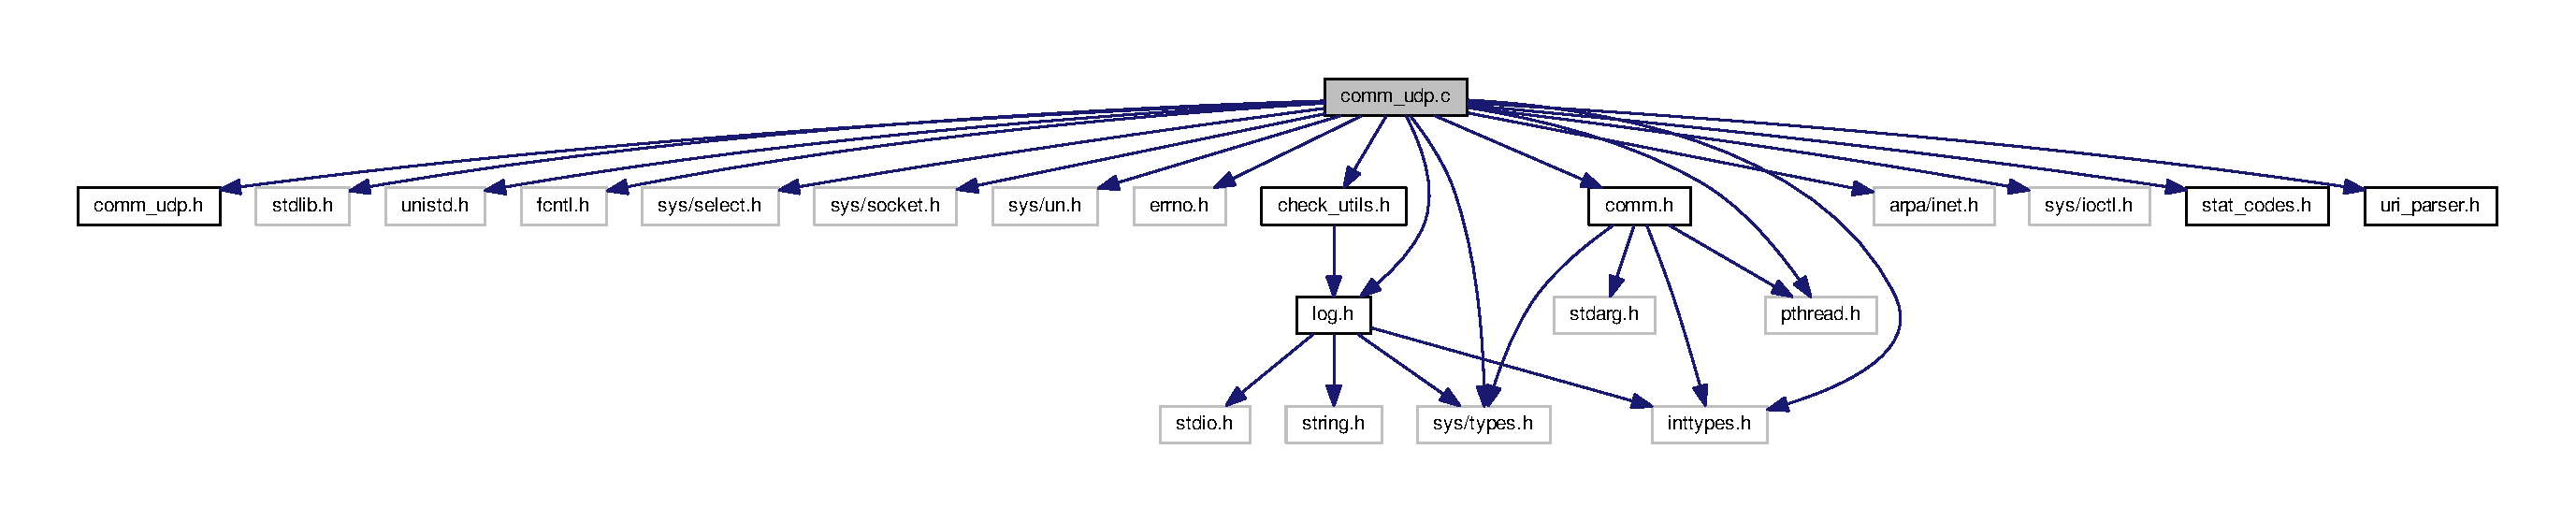
\includegraphics[width=350pt]{comm__udp_8c__incl}
\end{center}
\end{figure}
\subsection*{Classes}
\begin{DoxyCompactItemize}
\item 
struct \hyperlink{structcomm__udp__ctx__s}{comm\+\_\+udp\+\_\+ctx\+\_\+s}
\end{DoxyCompactItemize}
\subsection*{Macros}
\begin{DoxyCompactItemize}
\item 
\#define {\bfseries U\+D\+P\+\_\+\+C\+O\+M\+\_\+\+A\+D\+D\+R\+\_\+\+I\+S\+\_\+\+M\+U\+L\+T\+I\+C\+A\+ST}(addr)~I\+N\+\_\+\+M\+U\+L\+T\+I\+C\+A\+ST(htonl(addr))\hypertarget{comm__udp_8c_aa480ce3132c5b5d02061a7c0f183cb03}{}\label{comm__udp_8c_aa480ce3132c5b5d02061a7c0f183cb03}

\item 
\#define {\bfseries U\+D\+P\+\_\+\+C\+O\+M\+\_\+\+S\+O\+C\+K\+E\+T\+\_\+\+P\+R\+OT}~0\hypertarget{comm__udp_8c_aad39c4356310fc76a0e4429737fceac5}{}\label{comm__udp_8c_aad39c4356310fc76a0e4429737fceac5}

\item 
\#define {\bfseries U\+D\+P\+\_\+\+C\+O\+M\+\_\+\+D\+A\+T\+A\+G\+R\+A\+M\+\_\+\+B\+U\+F\+\_\+\+S\+I\+ZE}~(1024$\ast$1024$\ast$1024)\hypertarget{comm__udp_8c_a090368090d1eec4f9bf5f8c21e7bbbc3}{}\label{comm__udp_8c_a090368090d1eec4f9bf5f8c21e7bbbc3}

\end{DoxyCompactItemize}
\subsection*{Typedefs}
\begin{DoxyCompactItemize}
\item 
typedef struct \hyperlink{structcomm__udp__ctx__s}{comm\+\_\+udp\+\_\+ctx\+\_\+s} \hyperlink{comm__udp_8c_a6868f181bf22f0eaf2215d207f640428}{comm\+\_\+udp\+\_\+ctx\+\_\+t}
\end{DoxyCompactItemize}
\subsection*{Functions}
\begin{DoxyCompactItemize}
\item 
static \hyperlink{comm_8h_aacc0873718a86d8ef4658bad2500d091}{comm\+\_\+ctx\+\_\+t} $\ast$ {\bfseries comm\+\_\+udp\+\_\+open} (const char $\ast$url, const char $\ast$local\+\_\+url, \hyperlink{comm_8h_a2604d892f8ab29dfc96bd68e2cc3086f}{comm\+\_\+mode\+\_\+t} comm\+\_\+mode, \hyperlink{structlog__ctx__s}{log\+\_\+ctx\+\_\+t} $\ast$log\+\_\+ctx, va\+\_\+list arg)\hypertarget{comm__udp_8c_a033354dd1c48e420a26d52d540190e33}{}\label{comm__udp_8c_a033354dd1c48e420a26d52d540190e33}

\item 
static void {\bfseries comm\+\_\+udp\+\_\+close} (\hyperlink{comm_8h_aacc0873718a86d8ef4658bad2500d091}{comm\+\_\+ctx\+\_\+t} $\ast$$\ast$ref\+\_\+comm\+\_\+ctx)\hypertarget{comm__udp_8c_aabf0267a4b626412315fb0489ec342b8}{}\label{comm__udp_8c_aabf0267a4b626412315fb0489ec342b8}

\item 
static int {\bfseries comm\+\_\+udp\+\_\+send} (\hyperlink{comm_8h_aacc0873718a86d8ef4658bad2500d091}{comm\+\_\+ctx\+\_\+t} $\ast$comm\+\_\+ctx, const void $\ast$buf, size\+\_\+t count, struct timeval $\ast$timeout)\hypertarget{comm__udp_8c_a9a56fbbef77beab59be0f33a4bc00a34}{}\label{comm__udp_8c_a9a56fbbef77beab59be0f33a4bc00a34}

\item 
static int {\bfseries comm\+\_\+udp\+\_\+recv} (\hyperlink{comm_8h_aacc0873718a86d8ef4658bad2500d091}{comm\+\_\+ctx\+\_\+t} $\ast$comm\+\_\+ctx, void $\ast$$\ast$ref\+\_\+buf, size\+\_\+t $\ast$ref\+\_\+count, char $\ast$$\ast$ref\+\_\+from, struct timeval $\ast$timeout)\hypertarget{comm__udp_8c_a10563f454cef040d14edd5e7f04995a3}{}\label{comm__udp_8c_a10563f454cef040d14edd5e7f04995a3}

\item 
static int {\bfseries comm\+\_\+udp\+\_\+unblock} (\hyperlink{comm_8h_aacc0873718a86d8ef4658bad2500d091}{comm\+\_\+ctx\+\_\+t} $\ast$comm\+\_\+ctx)\hypertarget{comm__udp_8c_a84259e04cb1798e00e96587580d7d2f1}{}\label{comm__udp_8c_a84259e04cb1798e00e96587580d7d2f1}

\end{DoxyCompactItemize}
\subsection*{Variables}
\begin{DoxyCompactItemize}
\item 
const \hyperlink{comm_8h_a0d96b9368107e517ea8253837384faf5}{comm\+\_\+if\+\_\+t} \hyperlink{comm__udp_8c_abe388ee9ce49cba04e7c1adabf5ed9bc}{comm\+\_\+if\+\_\+udp}
\end{DoxyCompactItemize}


\subsection{Detailed Description}
\begin{DoxyAuthor}{Author}
Rafael Antoniello 
\end{DoxyAuthor}


\subsection{Typedef Documentation}
\index{comm\+\_\+udp.\+c@{comm\+\_\+udp.\+c}!comm\+\_\+udp\+\_\+ctx\+\_\+t@{comm\+\_\+udp\+\_\+ctx\+\_\+t}}
\index{comm\+\_\+udp\+\_\+ctx\+\_\+t@{comm\+\_\+udp\+\_\+ctx\+\_\+t}!comm\+\_\+udp.\+c@{comm\+\_\+udp.\+c}}
\subsubsection[{\texorpdfstring{comm\+\_\+udp\+\_\+ctx\+\_\+t}{comm_udp_ctx_t}}]{\setlength{\rightskip}{0pt plus 5cm}typedef struct {\bf comm\+\_\+udp\+\_\+ctx\+\_\+s}  {\bf comm\+\_\+udp\+\_\+ctx\+\_\+t}}\hypertarget{comm__udp_8c_a6868f181bf22f0eaf2215d207f640428}{}\label{comm__udp_8c_a6868f181bf22f0eaf2215d207f640428}
Module instance context structure 

\subsection{Variable Documentation}
\index{comm\+\_\+udp.\+c@{comm\+\_\+udp.\+c}!comm\+\_\+if\+\_\+udp@{comm\+\_\+if\+\_\+udp}}
\index{comm\+\_\+if\+\_\+udp@{comm\+\_\+if\+\_\+udp}!comm\+\_\+udp.\+c@{comm\+\_\+udp.\+c}}
\subsubsection[{\texorpdfstring{comm\+\_\+if\+\_\+udp}{comm_if_udp}}]{\setlength{\rightskip}{0pt plus 5cm}const {\bf comm\+\_\+if\+\_\+t} comm\+\_\+if\+\_\+udp}\hypertarget{comm__udp_8c_abe388ee9ce49cba04e7c1adabf5ed9bc}{}\label{comm__udp_8c_abe388ee9ce49cba04e7c1adabf5ed9bc}
{\bfseries Initial value\+:}
\begin{DoxyCode}
=
\{
    \textcolor{stringliteral}{"udp"},
    comm\_udp\_open,
    comm\_udp\_close,
    comm\_udp\_send,
    comm\_udp\_recv,
    comm\_udp\_unblock
\}
\end{DoxyCode}
Communication protocol interface implementing the User Data Protocol (U\+DP). 

Definition at line 102 of file comm\+\_\+udp.\+c.


\hypertarget{comm__udp_8h}{}\section{comm\+\_\+udp.\+h File Reference}
\label{comm__udp_8h}\index{comm\+\_\+udp.\+h@{comm\+\_\+udp.\+h}}


U\+DP communication module.  


This graph shows which files directly or indirectly include this file\+:\nopagebreak
\begin{figure}[H]
\begin{center}
\leavevmode
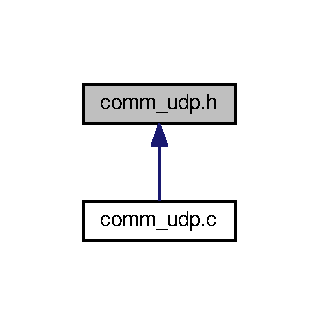
\includegraphics[width=153pt]{comm__udp_8h__dep__incl}
\end{center}
\end{figure}
\subsection*{Macros}
\begin{DoxyCompactItemize}
\item 
\#define \hyperlink{comm__udp_8h_ad2f8a5125fb9d8d152cf744c3876cd9d}{U\+D\+P\+\_\+\+C\+O\+M\+\_\+\+R\+E\+C\+V\+\_\+\+D\+G\+R\+A\+M\+\_\+\+M\+A\+X\+S\+I\+ZE}~2048
\end{DoxyCompactItemize}
\subsection*{Typedefs}
\begin{DoxyCompactItemize}
\item 
typedef struct \hyperlink{structcomm__if__s}{comm\+\_\+if\+\_\+s} {\bfseries comm\+\_\+if\+\_\+t}\hypertarget{comm__udp_8h_a27d1db6ede9956a35097bfc2a70f1991}{}\label{comm__udp_8h_a27d1db6ede9956a35097bfc2a70f1991}

\end{DoxyCompactItemize}
\subsection*{Variables}
\begin{DoxyCompactItemize}
\item 
const \hyperlink{comm_8h_a0d96b9368107e517ea8253837384faf5}{comm\+\_\+if\+\_\+t} \hyperlink{comm__udp_8h_abe388ee9ce49cba04e7c1adabf5ed9bc}{comm\+\_\+if\+\_\+udp}
\end{DoxyCompactItemize}


\subsection{Detailed Description}
U\+DP communication module. 

\begin{DoxyAuthor}{Author}
Rafael Antoniello 
\end{DoxyAuthor}


\subsection{Macro Definition Documentation}
\index{comm\+\_\+udp.\+h@{comm\+\_\+udp.\+h}!U\+D\+P\+\_\+\+C\+O\+M\+\_\+\+R\+E\+C\+V\+\_\+\+D\+G\+R\+A\+M\+\_\+\+M\+A\+X\+S\+I\+ZE@{U\+D\+P\+\_\+\+C\+O\+M\+\_\+\+R\+E\+C\+V\+\_\+\+D\+G\+R\+A\+M\+\_\+\+M\+A\+X\+S\+I\+ZE}}
\index{U\+D\+P\+\_\+\+C\+O\+M\+\_\+\+R\+E\+C\+V\+\_\+\+D\+G\+R\+A\+M\+\_\+\+M\+A\+X\+S\+I\+ZE@{U\+D\+P\+\_\+\+C\+O\+M\+\_\+\+R\+E\+C\+V\+\_\+\+D\+G\+R\+A\+M\+\_\+\+M\+A\+X\+S\+I\+ZE}!comm\+\_\+udp.\+h@{comm\+\_\+udp.\+h}}
\subsubsection[{\texorpdfstring{U\+D\+P\+\_\+\+C\+O\+M\+\_\+\+R\+E\+C\+V\+\_\+\+D\+G\+R\+A\+M\+\_\+\+M\+A\+X\+S\+I\+ZE}{UDP_COM_RECV_DGRAM_MAXSIZE}}]{\setlength{\rightskip}{0pt plus 5cm}\#define U\+D\+P\+\_\+\+C\+O\+M\+\_\+\+R\+E\+C\+V\+\_\+\+D\+G\+R\+A\+M\+\_\+\+M\+A\+X\+S\+I\+ZE~2048}\hypertarget{comm__udp_8h_ad2f8a5125fb9d8d152cf744c3876cd9d}{}\label{comm__udp_8h_ad2f8a5125fb9d8d152cf744c3876cd9d}
Maximum datagram size that can be received. 

Definition at line 44 of file comm\+\_\+udp.\+h.



\subsection{Variable Documentation}
\index{comm\+\_\+udp.\+h@{comm\+\_\+udp.\+h}!comm\+\_\+if\+\_\+udp@{comm\+\_\+if\+\_\+udp}}
\index{comm\+\_\+if\+\_\+udp@{comm\+\_\+if\+\_\+udp}!comm\+\_\+udp.\+h@{comm\+\_\+udp.\+h}}
\subsubsection[{\texorpdfstring{comm\+\_\+if\+\_\+udp}{comm_if_udp}}]{\setlength{\rightskip}{0pt plus 5cm}const {\bf comm\+\_\+if\+\_\+t} comm\+\_\+if\+\_\+udp}\hypertarget{comm__udp_8h_abe388ee9ce49cba04e7c1adabf5ed9bc}{}\label{comm__udp_8h_abe388ee9ce49cba04e7c1adabf5ed9bc}
Communication protocol interface implementing the User Data Protocol (U\+DP). 

Definition at line 102 of file comm\+\_\+udp.\+c.


\hypertarget{crc__32__mpeg2_8c}{}\section{crc\+\_\+32\+\_\+mpeg2.\+c File Reference}
\label{crc__32__mpeg2_8c}\index{crc\+\_\+32\+\_\+mpeg2.\+c@{crc\+\_\+32\+\_\+mpeg2.\+c}}
{\ttfamily \#include \char`\"{}crc\+\_\+32\+\_\+mpeg2.\+h\char`\"{}}\\*
{\ttfamily \#include $<$libmediaprocscrc/crc.\+h$>$}\\*
Include dependency graph for crc\+\_\+32\+\_\+mpeg2.\+c\+:\nopagebreak
\begin{figure}[H]
\begin{center}
\leavevmode
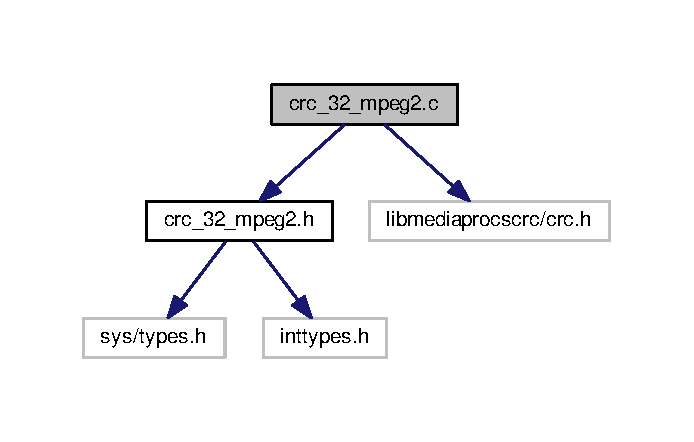
\includegraphics[width=333pt]{crc__32__mpeg2_8c__incl}
\end{center}
\end{figure}
\subsection*{Functions}
\begin{DoxyCompactItemize}
\item 
uint32\+\_\+t \hyperlink{crc__32__mpeg2_8c_ab4514110fdcfe3fc996d8fe71288b2a0}{crc\+\_\+32\+\_\+mpeg2} (uint8\+\_\+t $\ast$buf, uint16\+\_\+t size)
\end{DoxyCompactItemize}


\subsection{Detailed Description}
\begin{DoxyAuthor}{Author}
Rafael Antoniello 
\end{DoxyAuthor}


\subsection{Function Documentation}
\index{crc\+\_\+32\+\_\+mpeg2.\+c@{crc\+\_\+32\+\_\+mpeg2.\+c}!crc\+\_\+32\+\_\+mpeg2@{crc\+\_\+32\+\_\+mpeg2}}
\index{crc\+\_\+32\+\_\+mpeg2@{crc\+\_\+32\+\_\+mpeg2}!crc\+\_\+32\+\_\+mpeg2.\+c@{crc\+\_\+32\+\_\+mpeg2.\+c}}
\subsubsection[{\texorpdfstring{crc\+\_\+32\+\_\+mpeg2(uint8\+\_\+t $\ast$buf, uint16\+\_\+t size)}{crc_32_mpeg2(uint8_t *buf, uint16_t size)}}]{\setlength{\rightskip}{0pt plus 5cm}uint32\+\_\+t crc\+\_\+32\+\_\+mpeg2 (
\begin{DoxyParamCaption}
\item[{uint8\+\_\+t $\ast$}]{buf, }
\item[{uint16\+\_\+t}]{size}
\end{DoxyParamCaption}
)}\hypertarget{crc__32__mpeg2_8c_ab4514110fdcfe3fc996d8fe71288b2a0}{}\label{crc__32__mpeg2_8c_ab4514110fdcfe3fc996d8fe71288b2a0}
Check C\+R\+C-\/32 (3rd party library wrapper). 
\begin{DoxyParams}{Parameters}
{\em buf} & Input buffer pointer \\
\hline
{\em size} & Input buffer size in bytes \\
\hline
\end{DoxyParams}
\begin{DoxyReturn}{Returns}
C\+R\+C32 computation, as defined int I\+S\+O/\+I\+EC 13818-\/1, Annex A. 
\end{DoxyReturn}


Definition at line 38 of file crc\+\_\+32\+\_\+mpeg2.\+c.


\hypertarget{crc__32__mpeg2_8h}{}\section{crc\+\_\+32\+\_\+mpeg2.\+h File Reference}
\label{crc__32__mpeg2_8h}\index{crc\+\_\+32\+\_\+mpeg2.\+h@{crc\+\_\+32\+\_\+mpeg2.\+h}}


C\+R\+C-\/32 wrapper module.  


{\ttfamily \#include $<$sys/types.\+h$>$}\\*
{\ttfamily \#include $<$inttypes.\+h$>$}\\*
Include dependency graph for crc\+\_\+32\+\_\+mpeg2.\+h\+:\nopagebreak
\begin{figure}[H]
\begin{center}
\leavevmode
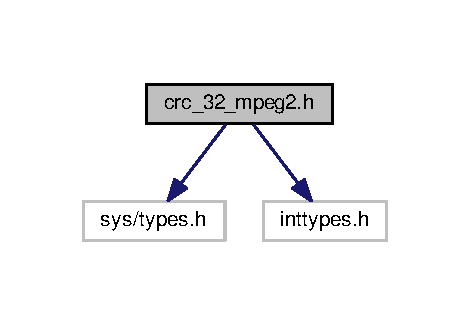
\includegraphics[width=226pt]{crc__32__mpeg2_8h__incl}
\end{center}
\end{figure}
This graph shows which files directly or indirectly include this file\+:\nopagebreak
\begin{figure}[H]
\begin{center}
\leavevmode
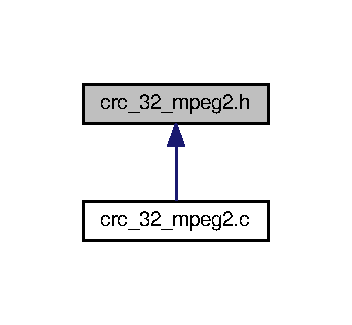
\includegraphics[width=169pt]{crc__32__mpeg2_8h__dep__incl}
\end{center}
\end{figure}
\subsection*{Functions}
\begin{DoxyCompactItemize}
\item 
uint32\+\_\+t \hyperlink{crc__32__mpeg2_8h_ab4514110fdcfe3fc996d8fe71288b2a0}{crc\+\_\+32\+\_\+mpeg2} (uint8\+\_\+t $\ast$buf, uint16\+\_\+t size)
\end{DoxyCompactItemize}


\subsection{Detailed Description}
C\+R\+C-\/32 wrapper module. 

\begin{DoxyAuthor}{Author}
Rafael Antoniello 
\end{DoxyAuthor}


\subsection{Function Documentation}
\index{crc\+\_\+32\+\_\+mpeg2.\+h@{crc\+\_\+32\+\_\+mpeg2.\+h}!crc\+\_\+32\+\_\+mpeg2@{crc\+\_\+32\+\_\+mpeg2}}
\index{crc\+\_\+32\+\_\+mpeg2@{crc\+\_\+32\+\_\+mpeg2}!crc\+\_\+32\+\_\+mpeg2.\+h@{crc\+\_\+32\+\_\+mpeg2.\+h}}
\subsubsection[{\texorpdfstring{crc\+\_\+32\+\_\+mpeg2(uint8\+\_\+t $\ast$buf, uint16\+\_\+t size)}{crc_32_mpeg2(uint8_t *buf, uint16_t size)}}]{\setlength{\rightskip}{0pt plus 5cm}uint32\+\_\+t crc\+\_\+32\+\_\+mpeg2 (
\begin{DoxyParamCaption}
\item[{uint8\+\_\+t $\ast$}]{buf, }
\item[{uint16\+\_\+t}]{size}
\end{DoxyParamCaption}
)}\hypertarget{crc__32__mpeg2_8h_ab4514110fdcfe3fc996d8fe71288b2a0}{}\label{crc__32__mpeg2_8h_ab4514110fdcfe3fc996d8fe71288b2a0}
Check C\+R\+C-\/32 (3rd party library wrapper). 
\begin{DoxyParams}{Parameters}
{\em buf} & Input buffer pointer \\
\hline
{\em size} & Input buffer size in bytes \\
\hline
\end{DoxyParams}
\begin{DoxyReturn}{Returns}
C\+R\+C32 computation, as defined int I\+S\+O/\+I\+EC 13818-\/1, Annex A. 
\end{DoxyReturn}


Definition at line 38 of file crc\+\_\+32\+\_\+mpeg2.\+c.


\input{fair__lock_8c}
\input{fair__lock_8h}
\hypertarget{ffmpeg__audio_8c}{}\section{ffmpeg\+\_\+audio.\+c File Reference}
\label{ffmpeg__audio_8c}\index{ffmpeg\+\_\+audio.\+c@{ffmpeg\+\_\+audio.\+c}}
{\ttfamily \#include \char`\"{}ffmpeg\+\_\+audio.\+h\char`\"{}}\\*
{\ttfamily \#include $<$stdlib.\+h$>$}\\*
{\ttfamily \#include $<$unistd.\+h$>$}\\*
{\ttfamily \#include $<$string.\+h$>$}\\*
{\ttfamily \#include $<$pthread.\+h$>$}\\*
{\ttfamily \#include $<$libavformat/avformat.\+h$>$}\\*
{\ttfamily \#include $<$libavcodec/avcodec.\+h$>$}\\*
{\ttfamily \#include $<$libavutil/mathematics.\+h$>$}\\*
{\ttfamily \#include $<$libavutil/opt.\+h$>$}\\*
{\ttfamily \#include $<$libswscale/swscale.\+h$>$}\\*
{\ttfamily \#include $<$libmediaprocsutils/log.\+h$>$}\\*
{\ttfamily \#include $<$libmediaprocsutils/stat\+\_\+codes.\+h$>$}\\*
{\ttfamily \#include $<$libmediaprocsutils/check\+\_\+utils.\+h$>$}\\*
{\ttfamily \#include $<$libmediaprocsutils/fair\+\_\+lock.\+h$>$}\\*
{\ttfamily \#include $<$libmediaprocsutils/fifo.\+h$>$}\\*
{\ttfamily \#include $<$libmediaprocs/proc\+\_\+if.\+h$>$}\\*
{\ttfamily \#include $<$libmediaprocs/proc.\+h$>$}\\*
{\ttfamily \#include \char`\"{}audio\+\_\+settings.\+h\char`\"{}}\\*
Include dependency graph for ffmpeg\+\_\+audio.\+c\+:\nopagebreak
\begin{figure}[H]
\begin{center}
\leavevmode
\includegraphics[width=350pt]{ffmpeg__audio_8c__incl}
\end{center}
\end{figure}
\subsection*{Macros}
\begin{DoxyCompactItemize}
\item 
\#define {\bfseries L\+O\+O\+P\+\_\+\+G\+U\+A\+R\+D\+\_\+\+M\+AX}~20\hypertarget{ffmpeg__audio_8c_aad7b6adebd4d452b00e9e0b5cec22cce}{}\label{ffmpeg__audio_8c_aad7b6adebd4d452b00e9e0b5cec22cce}

\end{DoxyCompactItemize}
\subsection*{Functions}
\begin{DoxyCompactItemize}
\item 
int \hyperlink{ffmpeg__audio_8c_a5ea9904072e0f6d4d8541c7b2e6aa9b1}{ffmpeg\+\_\+audio\+\_\+enc\+\_\+ctx\+\_\+init} (\hyperlink{ffmpeg__audio_8h_af0c12772b557383de7013dd6027c9159}{ffmpeg\+\_\+audio\+\_\+enc\+\_\+ctx\+\_\+t} $\ast$ffmpeg\+\_\+audio\+\_\+enc\+\_\+ctx, int avcodecid, const \hyperlink{audio__settings_8h_aef531d4a6946038cff191e1bd2f04e91}{audio\+\_\+settings\+\_\+enc\+\_\+ctx\+\_\+t} $\ast$audio\+\_\+settings\+\_\+enc\+\_\+ctx, \hyperlink{structlog__ctx__s}{log\+\_\+ctx\+\_\+t} $\ast$log\+\_\+ctx)
\item 
void \hyperlink{ffmpeg__audio_8c_aa637324b98054a600615fee6daef5210}{ffmpeg\+\_\+audio\+\_\+enc\+\_\+ctx\+\_\+deinit} (\hyperlink{ffmpeg__audio_8h_af0c12772b557383de7013dd6027c9159}{ffmpeg\+\_\+audio\+\_\+enc\+\_\+ctx\+\_\+t} $\ast$ffmpeg\+\_\+audio\+\_\+enc\+\_\+ctx, \hyperlink{structlog__ctx__s}{log\+\_\+ctx\+\_\+t} $\ast$log\+\_\+ctx)
\item 
int \hyperlink{ffmpeg__audio_8c_ac5fff0cac63a5f7321d1a5f5f5651cc3}{ffmpeg\+\_\+audio\+\_\+enc\+\_\+frame} (\hyperlink{ffmpeg__audio_8h_af0c12772b557383de7013dd6027c9159}{ffmpeg\+\_\+audio\+\_\+enc\+\_\+ctx\+\_\+t} $\ast$ffmpeg\+\_\+audio\+\_\+enc\+\_\+ctx, A\+V\+Frame $\ast$avframe\+\_\+iput, \hyperlink{fifo_8c_acf3f21e64cbabccd8420c306740820c1}{fifo\+\_\+ctx\+\_\+t} $\ast$oput\+\_\+fifo\+\_\+ctx, \hyperlink{structlog__ctx__s}{log\+\_\+ctx\+\_\+t} $\ast$log\+\_\+ctx)
\item 
int \hyperlink{ffmpeg__audio_8c_a536a23cea72fb5fe9c85a36c94f675eb}{ffmpeg\+\_\+audio\+\_\+dec\+\_\+ctx\+\_\+init} (\hyperlink{ffmpeg__audio_8h_a0c3f685b68ceba5d1e0b2d449f1c9ab9}{ffmpeg\+\_\+audio\+\_\+dec\+\_\+ctx\+\_\+t} $\ast$ffmpeg\+\_\+audio\+\_\+dec\+\_\+ctx, int avcodecid, const \hyperlink{audio__settings_8h_a1ec2b2e83ade2c4fc33cfb910bc007ad}{audio\+\_\+settings\+\_\+dec\+\_\+ctx\+\_\+t} $\ast$audio\+\_\+settings\+\_\+dec\+\_\+ctx, \hyperlink{structlog__ctx__s}{log\+\_\+ctx\+\_\+t} $\ast$log\+\_\+ctx)
\item 
void \hyperlink{ffmpeg__audio_8c_a8894753c3491a559764c560a0298d769}{ffmpeg\+\_\+audio\+\_\+dec\+\_\+ctx\+\_\+deinit} (\hyperlink{ffmpeg__audio_8h_a0c3f685b68ceba5d1e0b2d449f1c9ab9}{ffmpeg\+\_\+audio\+\_\+dec\+\_\+ctx\+\_\+t} $\ast$ffmpeg\+\_\+audio\+\_\+dec\+\_\+ctx, \hyperlink{structlog__ctx__s}{log\+\_\+ctx\+\_\+t} $\ast$log\+\_\+ctx)
\item 
int \hyperlink{ffmpeg__audio_8c_acef47e1a651e9b2d2ce572411832da3d}{ffmpeg\+\_\+audio\+\_\+dec\+\_\+frame} (\hyperlink{ffmpeg__audio_8h_a0c3f685b68ceba5d1e0b2d449f1c9ab9}{ffmpeg\+\_\+audio\+\_\+dec\+\_\+ctx\+\_\+t} $\ast$ffmpeg\+\_\+audio\+\_\+dec\+\_\+ctx, A\+V\+Packet $\ast$avpacket\+\_\+iput, \hyperlink{fifo_8c_acf3f21e64cbabccd8420c306740820c1}{fifo\+\_\+ctx\+\_\+t} $\ast$oput\+\_\+fifo\+\_\+ctx, \hyperlink{structlog__ctx__s}{log\+\_\+ctx\+\_\+t} $\ast$log\+\_\+ctx)
\item 
void \hyperlink{ffmpeg__audio_8c_aea2fe752df5b895e05beaa30aa7a4422}{ffmpeg\+\_\+audio\+\_\+reset\+\_\+on\+\_\+new\+\_\+settings} (\hyperlink{proc_8h_ae264f89be30fc03f5053bc16d58cba05}{proc\+\_\+ctx\+\_\+t} $\ast$proc\+\_\+ctx, volatile void $\ast$audio\+\_\+settings\+\_\+opaque, int flag\+\_\+is\+\_\+encoder, \hyperlink{structlog__ctx__s}{log\+\_\+ctx\+\_\+t} $\ast$log\+\_\+ctx)
\end{DoxyCompactItemize}


\subsection{Detailed Description}
\begin{DoxyAuthor}{Author}
Rafael Antoniello 
\end{DoxyAuthor}


\subsection{Function Documentation}
\index{ffmpeg\+\_\+audio.\+c@{ffmpeg\+\_\+audio.\+c}!ffmpeg\+\_\+audio\+\_\+dec\+\_\+ctx\+\_\+deinit@{ffmpeg\+\_\+audio\+\_\+dec\+\_\+ctx\+\_\+deinit}}
\index{ffmpeg\+\_\+audio\+\_\+dec\+\_\+ctx\+\_\+deinit@{ffmpeg\+\_\+audio\+\_\+dec\+\_\+ctx\+\_\+deinit}!ffmpeg\+\_\+audio.\+c@{ffmpeg\+\_\+audio.\+c}}
\subsubsection[{\texorpdfstring{ffmpeg\+\_\+audio\+\_\+dec\+\_\+ctx\+\_\+deinit(ffmpeg\+\_\+audio\+\_\+dec\+\_\+ctx\+\_\+t $\ast$ffmpeg\+\_\+audio\+\_\+dec\+\_\+ctx, log\+\_\+ctx\+\_\+t $\ast$log\+\_\+ctx)}{ffmpeg_audio_dec_ctx_deinit(ffmpeg_audio_dec_ctx_t *ffmpeg_audio_dec_ctx, log_ctx_t *log_ctx)}}]{\setlength{\rightskip}{0pt plus 5cm}void ffmpeg\+\_\+audio\+\_\+dec\+\_\+ctx\+\_\+deinit (
\begin{DoxyParamCaption}
\item[{{\bf ffmpeg\+\_\+audio\+\_\+dec\+\_\+ctx\+\_\+t} $\ast$}]{ffmpeg\+\_\+audio\+\_\+dec\+\_\+ctx, }
\item[{{\bf log\+\_\+ctx\+\_\+t} $\ast$}]{log\+\_\+ctx}
\end{DoxyParamCaption}
)}\hypertarget{ffmpeg__audio_8c_a8894753c3491a559764c560a0298d769}{}\label{ffmpeg__audio_8c_a8894753c3491a559764c560a0298d769}
De-\/initialize F\+Fmpeg\textquotesingle{}s audio decoding common context structure previously allocated by a call to \textquotesingle{}\hyperlink{ffmpeg__audio_8h_a536a23cea72fb5fe9c85a36c94f675eb}{ffmpeg\+\_\+audio\+\_\+dec\+\_\+ctx\+\_\+init()}\textquotesingle{}. This function release any heap-\/allocated field or structure member. 
\begin{DoxyParams}{Parameters}
{\em ffmpeg\+\_\+audio\+\_\+dec\+\_\+ctx} & Pointer to the audio decoding common context structure to be de-\/initialized. \\
\hline
{\em log\+\_\+ctx} & Externally defined L\+OG module context structure. \\
\hline
\end{DoxyParams}


Definition at line 301 of file ffmpeg\+\_\+audio.\+c.

\index{ffmpeg\+\_\+audio.\+c@{ffmpeg\+\_\+audio.\+c}!ffmpeg\+\_\+audio\+\_\+dec\+\_\+ctx\+\_\+init@{ffmpeg\+\_\+audio\+\_\+dec\+\_\+ctx\+\_\+init}}
\index{ffmpeg\+\_\+audio\+\_\+dec\+\_\+ctx\+\_\+init@{ffmpeg\+\_\+audio\+\_\+dec\+\_\+ctx\+\_\+init}!ffmpeg\+\_\+audio.\+c@{ffmpeg\+\_\+audio.\+c}}
\subsubsection[{\texorpdfstring{ffmpeg\+\_\+audio\+\_\+dec\+\_\+ctx\+\_\+init(ffmpeg\+\_\+audio\+\_\+dec\+\_\+ctx\+\_\+t $\ast$ffmpeg\+\_\+audio\+\_\+dec\+\_\+ctx, int avcodecid, const audio\+\_\+settings\+\_\+dec\+\_\+ctx\+\_\+t $\ast$audio\+\_\+settings\+\_\+dec\+\_\+ctx, log\+\_\+ctx\+\_\+t $\ast$log\+\_\+ctx)}{ffmpeg_audio_dec_ctx_init(ffmpeg_audio_dec_ctx_t *ffmpeg_audio_dec_ctx, int avcodecid, const audio_settings_dec_ctx_t *audio_settings_dec_ctx, log_ctx_t *log_ctx)}}]{\setlength{\rightskip}{0pt plus 5cm}int ffmpeg\+\_\+audio\+\_\+dec\+\_\+ctx\+\_\+init (
\begin{DoxyParamCaption}
\item[{{\bf ffmpeg\+\_\+audio\+\_\+dec\+\_\+ctx\+\_\+t} $\ast$}]{ffmpeg\+\_\+audio\+\_\+dec\+\_\+ctx, }
\item[{int}]{avcodecid, }
\item[{const {\bf audio\+\_\+settings\+\_\+dec\+\_\+ctx\+\_\+t} $\ast$}]{audio\+\_\+settings\+\_\+dec\+\_\+ctx, }
\item[{{\bf log\+\_\+ctx\+\_\+t} $\ast$}]{log\+\_\+ctx}
\end{DoxyParamCaption}
)}\hypertarget{ffmpeg__audio_8c_a536a23cea72fb5fe9c85a36c94f675eb}{}\label{ffmpeg__audio_8c_a536a23cea72fb5fe9c85a36c94f675eb}
Initialize F\+Fmpeg\textquotesingle{}s audio decoding common context structure. 
\begin{DoxyParams}{Parameters}
{\em ffmpeg\+\_\+audio\+\_\+dec\+\_\+ctx} & Pointer to the audio decoding common context structure to be initialized. \\
\hline
{\em avcodecid} & Unambiguous decoder identifier (namely, the decoder type Id.). \\
\hline
{\em audio\+\_\+settings\+\_\+dec\+\_\+ctx} & Pointer to the initial generic audio decoder settings context structure. \\
\hline
{\em log\+\_\+ctx} & Externally defined L\+OG module context structure. \\
\hline
\end{DoxyParams}
\begin{DoxyReturn}{Returns}
Status code (S\+T\+A\+T\+\_\+\+S\+U\+C\+C\+E\+SS code in case of success, for other code values please refer to .\hyperlink{stat__codes_8h}{stat\+\_\+codes.\+h}). 
\end{DoxyReturn}


Definition at line 229 of file ffmpeg\+\_\+audio.\+c.

\index{ffmpeg\+\_\+audio.\+c@{ffmpeg\+\_\+audio.\+c}!ffmpeg\+\_\+audio\+\_\+dec\+\_\+frame@{ffmpeg\+\_\+audio\+\_\+dec\+\_\+frame}}
\index{ffmpeg\+\_\+audio\+\_\+dec\+\_\+frame@{ffmpeg\+\_\+audio\+\_\+dec\+\_\+frame}!ffmpeg\+\_\+audio.\+c@{ffmpeg\+\_\+audio.\+c}}
\subsubsection[{\texorpdfstring{ffmpeg\+\_\+audio\+\_\+dec\+\_\+frame(ffmpeg\+\_\+audio\+\_\+dec\+\_\+ctx\+\_\+t $\ast$ffmpeg\+\_\+audio\+\_\+dec\+\_\+ctx, A\+V\+Packet $\ast$avpacket\+\_\+iput, fifo\+\_\+ctx\+\_\+t $\ast$oput\+\_\+fifo\+\_\+ctx, log\+\_\+ctx\+\_\+t $\ast$log\+\_\+ctx)}{ffmpeg_audio_dec_frame(ffmpeg_audio_dec_ctx_t *ffmpeg_audio_dec_ctx, AVPacket *avpacket_iput, fifo_ctx_t *oput_fifo_ctx, log_ctx_t *log_ctx)}}]{\setlength{\rightskip}{0pt plus 5cm}int ffmpeg\+\_\+audio\+\_\+dec\+\_\+frame (
\begin{DoxyParamCaption}
\item[{{\bf ffmpeg\+\_\+audio\+\_\+dec\+\_\+ctx\+\_\+t} $\ast$}]{ffmpeg\+\_\+audio\+\_\+dec\+\_\+ctx, }
\item[{A\+V\+Packet $\ast$}]{avpacket\+\_\+iput, }
\item[{{\bf fifo\+\_\+ctx\+\_\+t} $\ast$}]{oput\+\_\+fifo\+\_\+ctx, }
\item[{{\bf log\+\_\+ctx\+\_\+t} $\ast$}]{log\+\_\+ctx}
\end{DoxyParamCaption}
)}\hypertarget{ffmpeg__audio_8c_acef47e1a651e9b2d2ce572411832da3d}{}\label{ffmpeg__audio_8c_acef47e1a651e9b2d2ce572411832da3d}
Decode a complete audio frame. If an output frame is produced, is written to the output F\+I\+FO buffer. 
\begin{DoxyParams}{Parameters}
{\em ffmpeg\+\_\+audio\+\_\+dec\+\_\+ctx} & Pointer to the audio decoding common context structure. \\
\hline
{\em avpacket\+\_\+iput} & Pointer to the (F\+Fmpeg\textquotesingle{}s) input packet structure. \\
\hline
{\em oput\+\_\+fifo\+\_\+ctx} & Pointer to the output F\+I\+FO buffer context structure. \\
\hline
{\em log\+\_\+ctx} & Externally defined L\+OG module context structure. \\
\hline
\end{DoxyParams}
\begin{DoxyReturn}{Returns}
Status code (S\+T\+A\+T\+\_\+\+S\+U\+C\+C\+E\+SS code in case of success, for other code values please refer to .\hyperlink{stat__codes_8h}{stat\+\_\+codes.\+h}). 
\end{DoxyReturn}


Definition at line 311 of file ffmpeg\+\_\+audio.\+c.

\index{ffmpeg\+\_\+audio.\+c@{ffmpeg\+\_\+audio.\+c}!ffmpeg\+\_\+audio\+\_\+enc\+\_\+ctx\+\_\+deinit@{ffmpeg\+\_\+audio\+\_\+enc\+\_\+ctx\+\_\+deinit}}
\index{ffmpeg\+\_\+audio\+\_\+enc\+\_\+ctx\+\_\+deinit@{ffmpeg\+\_\+audio\+\_\+enc\+\_\+ctx\+\_\+deinit}!ffmpeg\+\_\+audio.\+c@{ffmpeg\+\_\+audio.\+c}}
\subsubsection[{\texorpdfstring{ffmpeg\+\_\+audio\+\_\+enc\+\_\+ctx\+\_\+deinit(ffmpeg\+\_\+audio\+\_\+enc\+\_\+ctx\+\_\+t $\ast$ffmpeg\+\_\+audio\+\_\+enc\+\_\+ctx, log\+\_\+ctx\+\_\+t $\ast$log\+\_\+ctx)}{ffmpeg_audio_enc_ctx_deinit(ffmpeg_audio_enc_ctx_t *ffmpeg_audio_enc_ctx, log_ctx_t *log_ctx)}}]{\setlength{\rightskip}{0pt plus 5cm}void ffmpeg\+\_\+audio\+\_\+enc\+\_\+ctx\+\_\+deinit (
\begin{DoxyParamCaption}
\item[{{\bf ffmpeg\+\_\+audio\+\_\+enc\+\_\+ctx\+\_\+t} $\ast$}]{ffmpeg\+\_\+audio\+\_\+enc\+\_\+ctx, }
\item[{{\bf log\+\_\+ctx\+\_\+t} $\ast$}]{log\+\_\+ctx}
\end{DoxyParamCaption}
)}\hypertarget{ffmpeg__audio_8c_aa637324b98054a600615fee6daef5210}{}\label{ffmpeg__audio_8c_aa637324b98054a600615fee6daef5210}
De-\/initialize F\+Fmpeg\textquotesingle{}s audio encoding common context structure previously allocated by a call to \textquotesingle{}\hyperlink{ffmpeg__audio_8h_a5ea9904072e0f6d4d8541c7b2e6aa9b1}{ffmpeg\+\_\+audio\+\_\+enc\+\_\+ctx\+\_\+init()}\textquotesingle{}. This function release any heap-\/allocated field or structure member. 
\begin{DoxyParams}{Parameters}
{\em ffmpeg\+\_\+audio\+\_\+enc\+\_\+ctx} & Pointer to the audio encoding common context structure to be de-\/initialized. \\
\hline
{\em log\+\_\+ctx} & Externally defined L\+OG module context structure. \\
\hline
\end{DoxyParams}


Definition at line 139 of file ffmpeg\+\_\+audio.\+c.

\index{ffmpeg\+\_\+audio.\+c@{ffmpeg\+\_\+audio.\+c}!ffmpeg\+\_\+audio\+\_\+enc\+\_\+ctx\+\_\+init@{ffmpeg\+\_\+audio\+\_\+enc\+\_\+ctx\+\_\+init}}
\index{ffmpeg\+\_\+audio\+\_\+enc\+\_\+ctx\+\_\+init@{ffmpeg\+\_\+audio\+\_\+enc\+\_\+ctx\+\_\+init}!ffmpeg\+\_\+audio.\+c@{ffmpeg\+\_\+audio.\+c}}
\subsubsection[{\texorpdfstring{ffmpeg\+\_\+audio\+\_\+enc\+\_\+ctx\+\_\+init(ffmpeg\+\_\+audio\+\_\+enc\+\_\+ctx\+\_\+t $\ast$ffmpeg\+\_\+audio\+\_\+enc\+\_\+ctx, int avcodecid, const audio\+\_\+settings\+\_\+enc\+\_\+ctx\+\_\+t $\ast$audio\+\_\+settings\+\_\+enc\+\_\+ctx, log\+\_\+ctx\+\_\+t $\ast$log\+\_\+ctx)}{ffmpeg_audio_enc_ctx_init(ffmpeg_audio_enc_ctx_t *ffmpeg_audio_enc_ctx, int avcodecid, const audio_settings_enc_ctx_t *audio_settings_enc_ctx, log_ctx_t *log_ctx)}}]{\setlength{\rightskip}{0pt plus 5cm}int ffmpeg\+\_\+audio\+\_\+enc\+\_\+ctx\+\_\+init (
\begin{DoxyParamCaption}
\item[{{\bf ffmpeg\+\_\+audio\+\_\+enc\+\_\+ctx\+\_\+t} $\ast$}]{ffmpeg\+\_\+audio\+\_\+enc\+\_\+ctx, }
\item[{int}]{avcodecid, }
\item[{const {\bf audio\+\_\+settings\+\_\+enc\+\_\+ctx\+\_\+t} $\ast$}]{audio\+\_\+settings\+\_\+enc\+\_\+ctx, }
\item[{{\bf log\+\_\+ctx\+\_\+t} $\ast$}]{log\+\_\+ctx}
\end{DoxyParamCaption}
)}\hypertarget{ffmpeg__audio_8c_a5ea9904072e0f6d4d8541c7b2e6aa9b1}{}\label{ffmpeg__audio_8c_a5ea9904072e0f6d4d8541c7b2e6aa9b1}
Initialize F\+Fmpeg\textquotesingle{}s audio encoding common context structure. 
\begin{DoxyParams}{Parameters}
{\em ffmpeg\+\_\+audio\+\_\+enc\+\_\+ctx} & Pointer to the audio encoding common context structure to be initialized. \\
\hline
{\em avcodecid} & Unambiguous encoder identifier (namely, the encoder type Id.). \\
\hline
{\em audio\+\_\+settings\+\_\+enc\+\_\+ctx} & Pointer to the initial generic audio encoder settings context structure. \\
\hline
{\em log\+\_\+ctx} & Externally defined L\+OG module context structure. \\
\hline
\end{DoxyParams}
\begin{DoxyReturn}{Returns}
Status code (S\+T\+A\+T\+\_\+\+S\+U\+C\+C\+E\+SS code in case of success, for other code values please refer to .\hyperlink{stat__codes_8h}{stat\+\_\+codes.\+h}). 
\end{DoxyReturn}


Definition at line 55 of file ffmpeg\+\_\+audio.\+c.

\index{ffmpeg\+\_\+audio.\+c@{ffmpeg\+\_\+audio.\+c}!ffmpeg\+\_\+audio\+\_\+enc\+\_\+frame@{ffmpeg\+\_\+audio\+\_\+enc\+\_\+frame}}
\index{ffmpeg\+\_\+audio\+\_\+enc\+\_\+frame@{ffmpeg\+\_\+audio\+\_\+enc\+\_\+frame}!ffmpeg\+\_\+audio.\+c@{ffmpeg\+\_\+audio.\+c}}
\subsubsection[{\texorpdfstring{ffmpeg\+\_\+audio\+\_\+enc\+\_\+frame(ffmpeg\+\_\+audio\+\_\+enc\+\_\+ctx\+\_\+t $\ast$ffmpeg\+\_\+audio\+\_\+enc\+\_\+ctx, A\+V\+Frame $\ast$avframe\+\_\+iput, fifo\+\_\+ctx\+\_\+t $\ast$oput\+\_\+fifo\+\_\+ctx, log\+\_\+ctx\+\_\+t $\ast$log\+\_\+ctx)}{ffmpeg_audio_enc_frame(ffmpeg_audio_enc_ctx_t *ffmpeg_audio_enc_ctx, AVFrame *avframe_iput, fifo_ctx_t *oput_fifo_ctx, log_ctx_t *log_ctx)}}]{\setlength{\rightskip}{0pt plus 5cm}int ffmpeg\+\_\+audio\+\_\+enc\+\_\+frame (
\begin{DoxyParamCaption}
\item[{{\bf ffmpeg\+\_\+audio\+\_\+enc\+\_\+ctx\+\_\+t} $\ast$}]{ffmpeg\+\_\+audio\+\_\+enc\+\_\+ctx, }
\item[{A\+V\+Frame $\ast$}]{avframe\+\_\+iput, }
\item[{{\bf fifo\+\_\+ctx\+\_\+t} $\ast$}]{oput\+\_\+fifo\+\_\+ctx, }
\item[{{\bf log\+\_\+ctx\+\_\+t} $\ast$}]{log\+\_\+ctx}
\end{DoxyParamCaption}
)}\hypertarget{ffmpeg__audio_8c_ac5fff0cac63a5f7321d1a5f5f5651cc3}{}\label{ffmpeg__audio_8c_ac5fff0cac63a5f7321d1a5f5f5651cc3}
Encode a complete audio frame. If an output frame is produced, is written to the output F\+I\+FO buffer. 
\begin{DoxyParams}{Parameters}
{\em ffmpeg\+\_\+audio\+\_\+enc\+\_\+ctx} & Pointer to the audio encoding common context structure. \\
\hline
{\em avframe\+\_\+iput} & Pointer to the (F\+Fmpeg\textquotesingle{}s) input frame structure. \\
\hline
{\em oput\+\_\+fifo\+\_\+ctx} & Pointer to the output F\+I\+FO buffer context structure. \\
\hline
{\em log\+\_\+ctx} & Externally defined L\+OG module context structure. \\
\hline
\end{DoxyParams}
\begin{DoxyReturn}{Returns}
Status code (S\+T\+A\+T\+\_\+\+S\+U\+C\+C\+E\+SS code in case of success, for other code values please refer to .\hyperlink{stat__codes_8h}{stat\+\_\+codes.\+h}). 
\end{DoxyReturn}


Definition at line 149 of file ffmpeg\+\_\+audio.\+c.

\index{ffmpeg\+\_\+audio.\+c@{ffmpeg\+\_\+audio.\+c}!ffmpeg\+\_\+audio\+\_\+reset\+\_\+on\+\_\+new\+\_\+settings@{ffmpeg\+\_\+audio\+\_\+reset\+\_\+on\+\_\+new\+\_\+settings}}
\index{ffmpeg\+\_\+audio\+\_\+reset\+\_\+on\+\_\+new\+\_\+settings@{ffmpeg\+\_\+audio\+\_\+reset\+\_\+on\+\_\+new\+\_\+settings}!ffmpeg\+\_\+audio.\+c@{ffmpeg\+\_\+audio.\+c}}
\subsubsection[{\texorpdfstring{ffmpeg\+\_\+audio\+\_\+reset\+\_\+on\+\_\+new\+\_\+settings(proc\+\_\+ctx\+\_\+t $\ast$proc\+\_\+ctx, volatile void $\ast$audio\+\_\+settings\+\_\+opaque, int flag\+\_\+is\+\_\+encoder, log\+\_\+ctx\+\_\+t $\ast$log\+\_\+ctx)}{ffmpeg_audio_reset_on_new_settings(proc_ctx_t *proc_ctx, volatile void *audio_settings_opaque, int flag_is_encoder, log_ctx_t *log_ctx)}}]{\setlength{\rightskip}{0pt plus 5cm}void ffmpeg\+\_\+audio\+\_\+reset\+\_\+on\+\_\+new\+\_\+settings (
\begin{DoxyParamCaption}
\item[{{\bf proc\+\_\+ctx\+\_\+t} $\ast$}]{proc\+\_\+ctx, }
\item[{volatile void $\ast$}]{audio\+\_\+settings\+\_\+opaque, }
\item[{int}]{flag\+\_\+is\+\_\+encoder, }
\item[{{\bf log\+\_\+ctx\+\_\+t} $\ast$}]{log\+\_\+ctx}
\end{DoxyParamCaption}
)}\hypertarget{ffmpeg__audio_8c_aea2fe752df5b895e05beaa30aa7a4422}{}\label{ffmpeg__audio_8c_aea2fe752df5b895e05beaa30aa7a4422}
F\+Fmpeg audio C\+O\+D\+E\+CS are not generally designed to accept changing settings on run-\/time. Thus, we have to reset (that is, de-\/initialize and re-\/initialize) the C\+O\+D\+EC to set new settings while running the processor. 
\begin{DoxyParams}{Parameters}
{\em proc\+\_\+ctx} & Pointer to the processor (P\+R\+OC) context structure \\
\hline
{\em audio\+\_\+settings\+\_\+opaque} & Opaque pointer to be casted either to an encoder or decoder audio settings context structure. \\
\hline
{\em flag\+\_\+is\+\_\+encoder} & Set to non-\/zero to signal that we are resetting an encoder, set to zero to identify a decoder. \\
\hline
{\em log\+\_\+ctx} & Pointer to the L\+OG module context structure. \\
\hline
\end{DoxyParams}


Definition at line 392 of file ffmpeg\+\_\+audio.\+c.


\hypertarget{ffmpeg__audio_8h}{}\section{ffmpeg\+\_\+audio.\+h File Reference}
\label{ffmpeg__audio_8h}\index{ffmpeg\+\_\+audio.\+h@{ffmpeg\+\_\+audio.\+h}}


Generic processor module context (see type proc\+\_\+ctx\+\_\+t) extension for audio encoders and decoders.  


{\ttfamily \#include $<$libmediaprocsutils/mem\+\_\+utils.\+h$>$}\\*
{\ttfamily \#include $<$libmediaprocs/proc.\+h$>$}\\*
Include dependency graph for ffmpeg\+\_\+audio.\+h\+:\nopagebreak
\begin{figure}[H]
\begin{center}
\leavevmode
\includegraphics[width=300pt]{ffmpeg__audio_8h__incl}
\end{center}
\end{figure}
This graph shows which files directly or indirectly include this file\+:\nopagebreak
\begin{figure}[H]
\begin{center}
\leavevmode
\includegraphics[width=260pt]{ffmpeg__audio_8h__dep__incl}
\end{center}
\end{figure}
\subsection*{Classes}
\begin{DoxyCompactItemize}
\item 
struct \hyperlink{structffmpeg__audio__enc__ctx__s}{ffmpeg\+\_\+audio\+\_\+enc\+\_\+ctx\+\_\+s}
\item 
struct \hyperlink{structffmpeg__audio__dec__ctx__s}{ffmpeg\+\_\+audio\+\_\+dec\+\_\+ctx\+\_\+s}
\end{DoxyCompactItemize}
\subsection*{Typedefs}
\begin{DoxyCompactItemize}
\item 
typedef struct A\+V\+Codec {\bfseries A\+V\+Codec}\hypertarget{ffmpeg__audio_8h_a87fe4be69cf6184ee6e6f96828de9735}{}\label{ffmpeg__audio_8h_a87fe4be69cf6184ee6e6f96828de9735}

\item 
typedef struct A\+V\+Codec\+Context {\bfseries A\+V\+Codec\+Context}\hypertarget{ffmpeg__audio_8h_ac9ee855329a1cfa5ebbbf2f819a39a6a}{}\label{ffmpeg__audio_8h_ac9ee855329a1cfa5ebbbf2f819a39a6a}

\item 
typedef struct A\+V\+Frame {\bfseries A\+V\+Frame}\hypertarget{ffmpeg__audio_8h_adb9d87a8956751b4fd71791105d65c52}{}\label{ffmpeg__audio_8h_adb9d87a8956751b4fd71791105d65c52}

\item 
typedef struct A\+V\+Packet {\bfseries A\+V\+Packet}\hypertarget{ffmpeg__audio_8h_a95fb1cffcaba889eaca3b985c811991b}{}\label{ffmpeg__audio_8h_a95fb1cffcaba889eaca3b985c811991b}

\item 
typedef struct \hyperlink{structaudio__settings__enc__ctx__s}{audio\+\_\+settings\+\_\+enc\+\_\+ctx\+\_\+s} {\bfseries audio\+\_\+settings\+\_\+enc\+\_\+ctx\+\_\+t}\hypertarget{ffmpeg__audio_8h_a3e020bcff532baef0cc2c3b29a167ce6}{}\label{ffmpeg__audio_8h_a3e020bcff532baef0cc2c3b29a167ce6}

\item 
typedef struct \hyperlink{structaudio__settings__dec__ctx__s}{audio\+\_\+settings\+\_\+dec\+\_\+ctx\+\_\+s} {\bfseries audio\+\_\+settings\+\_\+dec\+\_\+ctx\+\_\+t}\hypertarget{ffmpeg__audio_8h_a80b71f003a523e226fe728f26a5b7fc4}{}\label{ffmpeg__audio_8h_a80b71f003a523e226fe728f26a5b7fc4}

\item 
typedef struct \hyperlink{structffmpeg__audio__enc__ctx__s}{ffmpeg\+\_\+audio\+\_\+enc\+\_\+ctx\+\_\+s} \hyperlink{ffmpeg__audio_8h_af0c12772b557383de7013dd6027c9159}{ffmpeg\+\_\+audio\+\_\+enc\+\_\+ctx\+\_\+t}
\item 
typedef struct \hyperlink{structffmpeg__audio__dec__ctx__s}{ffmpeg\+\_\+audio\+\_\+dec\+\_\+ctx\+\_\+s} \hyperlink{ffmpeg__audio_8h_a0c3f685b68ceba5d1e0b2d449f1c9ab9}{ffmpeg\+\_\+audio\+\_\+dec\+\_\+ctx\+\_\+t}
\end{DoxyCompactItemize}
\subsection*{Functions}
\begin{DoxyCompactItemize}
\item 
int \hyperlink{ffmpeg__audio_8h_a5ea9904072e0f6d4d8541c7b2e6aa9b1}{ffmpeg\+\_\+audio\+\_\+enc\+\_\+ctx\+\_\+init} (\hyperlink{ffmpeg__audio_8h_af0c12772b557383de7013dd6027c9159}{ffmpeg\+\_\+audio\+\_\+enc\+\_\+ctx\+\_\+t} $\ast$ffmpeg\+\_\+audio\+\_\+enc\+\_\+ctx, int avcodecid, const \hyperlink{audio__settings_8h_aef531d4a6946038cff191e1bd2f04e91}{audio\+\_\+settings\+\_\+enc\+\_\+ctx\+\_\+t} $\ast$audio\+\_\+settings\+\_\+enc\+\_\+ctx, \hyperlink{structlog__ctx__s}{log\+\_\+ctx\+\_\+t} $\ast$log\+\_\+ctx)
\item 
void \hyperlink{ffmpeg__audio_8h_aa637324b98054a600615fee6daef5210}{ffmpeg\+\_\+audio\+\_\+enc\+\_\+ctx\+\_\+deinit} (\hyperlink{ffmpeg__audio_8h_af0c12772b557383de7013dd6027c9159}{ffmpeg\+\_\+audio\+\_\+enc\+\_\+ctx\+\_\+t} $\ast$ffmpeg\+\_\+audio\+\_\+enc\+\_\+ctx, \hyperlink{structlog__ctx__s}{log\+\_\+ctx\+\_\+t} $\ast$log\+\_\+ctx)
\item 
int \hyperlink{ffmpeg__audio_8h_ac5fff0cac63a5f7321d1a5f5f5651cc3}{ffmpeg\+\_\+audio\+\_\+enc\+\_\+frame} (\hyperlink{ffmpeg__audio_8h_af0c12772b557383de7013dd6027c9159}{ffmpeg\+\_\+audio\+\_\+enc\+\_\+ctx\+\_\+t} $\ast$ffmpeg\+\_\+audio\+\_\+enc\+\_\+ctx, A\+V\+Frame $\ast$avframe\+\_\+iput, \hyperlink{fifo_8c_acf3f21e64cbabccd8420c306740820c1}{fifo\+\_\+ctx\+\_\+t} $\ast$oput\+\_\+fifo\+\_\+ctx, \hyperlink{structlog__ctx__s}{log\+\_\+ctx\+\_\+t} $\ast$log\+\_\+ctx)
\item 
int \hyperlink{ffmpeg__audio_8h_a536a23cea72fb5fe9c85a36c94f675eb}{ffmpeg\+\_\+audio\+\_\+dec\+\_\+ctx\+\_\+init} (\hyperlink{ffmpeg__audio_8h_a0c3f685b68ceba5d1e0b2d449f1c9ab9}{ffmpeg\+\_\+audio\+\_\+dec\+\_\+ctx\+\_\+t} $\ast$ffmpeg\+\_\+audio\+\_\+dec\+\_\+ctx, int avcodecid, const \hyperlink{audio__settings_8h_a1ec2b2e83ade2c4fc33cfb910bc007ad}{audio\+\_\+settings\+\_\+dec\+\_\+ctx\+\_\+t} $\ast$audio\+\_\+settings\+\_\+dec\+\_\+ctx, \hyperlink{structlog__ctx__s}{log\+\_\+ctx\+\_\+t} $\ast$log\+\_\+ctx)
\item 
void \hyperlink{ffmpeg__audio_8h_a8894753c3491a559764c560a0298d769}{ffmpeg\+\_\+audio\+\_\+dec\+\_\+ctx\+\_\+deinit} (\hyperlink{ffmpeg__audio_8h_a0c3f685b68ceba5d1e0b2d449f1c9ab9}{ffmpeg\+\_\+audio\+\_\+dec\+\_\+ctx\+\_\+t} $\ast$ffmpeg\+\_\+audio\+\_\+dec\+\_\+ctx, \hyperlink{structlog__ctx__s}{log\+\_\+ctx\+\_\+t} $\ast$log\+\_\+ctx)
\item 
int \hyperlink{ffmpeg__audio_8h_acef47e1a651e9b2d2ce572411832da3d}{ffmpeg\+\_\+audio\+\_\+dec\+\_\+frame} (\hyperlink{ffmpeg__audio_8h_a0c3f685b68ceba5d1e0b2d449f1c9ab9}{ffmpeg\+\_\+audio\+\_\+dec\+\_\+ctx\+\_\+t} $\ast$ffmpeg\+\_\+audio\+\_\+dec\+\_\+ctx, A\+V\+Packet $\ast$avpacket\+\_\+iput, \hyperlink{fifo_8c_acf3f21e64cbabccd8420c306740820c1}{fifo\+\_\+ctx\+\_\+t} $\ast$oput\+\_\+fifo\+\_\+ctx, \hyperlink{structlog__ctx__s}{log\+\_\+ctx\+\_\+t} $\ast$log\+\_\+ctx)
\item 
void \hyperlink{ffmpeg__audio_8h_aea2fe752df5b895e05beaa30aa7a4422}{ffmpeg\+\_\+audio\+\_\+reset\+\_\+on\+\_\+new\+\_\+settings} (\hyperlink{proc_8h_ae264f89be30fc03f5053bc16d58cba05}{proc\+\_\+ctx\+\_\+t} $\ast$proc\+\_\+ctx, volatile void $\ast$audio\+\_\+settings\+\_\+opaque, int flag\+\_\+is\+\_\+encoder, \hyperlink{structlog__ctx__s}{log\+\_\+ctx\+\_\+t} $\ast$log\+\_\+ctx)
\end{DoxyCompactItemize}


\subsection{Detailed Description}
Generic processor module context (see type proc\+\_\+ctx\+\_\+t) extension for audio encoders and decoders. 

\begin{DoxyAuthor}{Author}
Rafael Antoniello 
\end{DoxyAuthor}


\subsection{Typedef Documentation}
\index{ffmpeg\+\_\+audio.\+h@{ffmpeg\+\_\+audio.\+h}!ffmpeg\+\_\+audio\+\_\+dec\+\_\+ctx\+\_\+t@{ffmpeg\+\_\+audio\+\_\+dec\+\_\+ctx\+\_\+t}}
\index{ffmpeg\+\_\+audio\+\_\+dec\+\_\+ctx\+\_\+t@{ffmpeg\+\_\+audio\+\_\+dec\+\_\+ctx\+\_\+t}!ffmpeg\+\_\+audio.\+h@{ffmpeg\+\_\+audio.\+h}}
\subsubsection[{\texorpdfstring{ffmpeg\+\_\+audio\+\_\+dec\+\_\+ctx\+\_\+t}{ffmpeg_audio_dec_ctx_t}}]{\setlength{\rightskip}{0pt plus 5cm}typedef struct {\bf ffmpeg\+\_\+audio\+\_\+dec\+\_\+ctx\+\_\+s}  {\bf ffmpeg\+\_\+audio\+\_\+dec\+\_\+ctx\+\_\+t}}\hypertarget{ffmpeg__audio_8h_a0c3f685b68ceba5d1e0b2d449f1c9ab9}{}\label{ffmpeg__audio_8h_a0c3f685b68ceba5d1e0b2d449f1c9ab9}
F\+Fmpeg audio decoding common context structure. \index{ffmpeg\+\_\+audio.\+h@{ffmpeg\+\_\+audio.\+h}!ffmpeg\+\_\+audio\+\_\+enc\+\_\+ctx\+\_\+t@{ffmpeg\+\_\+audio\+\_\+enc\+\_\+ctx\+\_\+t}}
\index{ffmpeg\+\_\+audio\+\_\+enc\+\_\+ctx\+\_\+t@{ffmpeg\+\_\+audio\+\_\+enc\+\_\+ctx\+\_\+t}!ffmpeg\+\_\+audio.\+h@{ffmpeg\+\_\+audio.\+h}}
\subsubsection[{\texorpdfstring{ffmpeg\+\_\+audio\+\_\+enc\+\_\+ctx\+\_\+t}{ffmpeg_audio_enc_ctx_t}}]{\setlength{\rightskip}{0pt plus 5cm}typedef struct {\bf ffmpeg\+\_\+audio\+\_\+enc\+\_\+ctx\+\_\+s}  {\bf ffmpeg\+\_\+audio\+\_\+enc\+\_\+ctx\+\_\+t}}\hypertarget{ffmpeg__audio_8h_af0c12772b557383de7013dd6027c9159}{}\label{ffmpeg__audio_8h_af0c12772b557383de7013dd6027c9159}
F\+Fmpeg audio encoding common context structure. 

\subsection{Function Documentation}
\index{ffmpeg\+\_\+audio.\+h@{ffmpeg\+\_\+audio.\+h}!ffmpeg\+\_\+audio\+\_\+dec\+\_\+ctx\+\_\+deinit@{ffmpeg\+\_\+audio\+\_\+dec\+\_\+ctx\+\_\+deinit}}
\index{ffmpeg\+\_\+audio\+\_\+dec\+\_\+ctx\+\_\+deinit@{ffmpeg\+\_\+audio\+\_\+dec\+\_\+ctx\+\_\+deinit}!ffmpeg\+\_\+audio.\+h@{ffmpeg\+\_\+audio.\+h}}
\subsubsection[{\texorpdfstring{ffmpeg\+\_\+audio\+\_\+dec\+\_\+ctx\+\_\+deinit(ffmpeg\+\_\+audio\+\_\+dec\+\_\+ctx\+\_\+t $\ast$ffmpeg\+\_\+audio\+\_\+dec\+\_\+ctx, log\+\_\+ctx\+\_\+t $\ast$log\+\_\+ctx)}{ffmpeg_audio_dec_ctx_deinit(ffmpeg_audio_dec_ctx_t *ffmpeg_audio_dec_ctx, log_ctx_t *log_ctx)}}]{\setlength{\rightskip}{0pt plus 5cm}void ffmpeg\+\_\+audio\+\_\+dec\+\_\+ctx\+\_\+deinit (
\begin{DoxyParamCaption}
\item[{{\bf ffmpeg\+\_\+audio\+\_\+dec\+\_\+ctx\+\_\+t} $\ast$}]{ffmpeg\+\_\+audio\+\_\+dec\+\_\+ctx, }
\item[{{\bf log\+\_\+ctx\+\_\+t} $\ast$}]{log\+\_\+ctx}
\end{DoxyParamCaption}
)}\hypertarget{ffmpeg__audio_8h_a8894753c3491a559764c560a0298d769}{}\label{ffmpeg__audio_8h_a8894753c3491a559764c560a0298d769}
De-\/initialize F\+Fmpeg\textquotesingle{}s audio decoding common context structure previously allocated by a call to \textquotesingle{}\hyperlink{ffmpeg__audio_8h_a536a23cea72fb5fe9c85a36c94f675eb}{ffmpeg\+\_\+audio\+\_\+dec\+\_\+ctx\+\_\+init()}\textquotesingle{}. This function release any heap-\/allocated field or structure member. 
\begin{DoxyParams}{Parameters}
{\em ffmpeg\+\_\+audio\+\_\+dec\+\_\+ctx} & Pointer to the audio decoding common context structure to be de-\/initialized. \\
\hline
{\em log\+\_\+ctx} & Externally defined L\+OG module context structure. \\
\hline
\end{DoxyParams}


Definition at line 301 of file ffmpeg\+\_\+audio.\+c.

\index{ffmpeg\+\_\+audio.\+h@{ffmpeg\+\_\+audio.\+h}!ffmpeg\+\_\+audio\+\_\+dec\+\_\+ctx\+\_\+init@{ffmpeg\+\_\+audio\+\_\+dec\+\_\+ctx\+\_\+init}}
\index{ffmpeg\+\_\+audio\+\_\+dec\+\_\+ctx\+\_\+init@{ffmpeg\+\_\+audio\+\_\+dec\+\_\+ctx\+\_\+init}!ffmpeg\+\_\+audio.\+h@{ffmpeg\+\_\+audio.\+h}}
\subsubsection[{\texorpdfstring{ffmpeg\+\_\+audio\+\_\+dec\+\_\+ctx\+\_\+init(ffmpeg\+\_\+audio\+\_\+dec\+\_\+ctx\+\_\+t $\ast$ffmpeg\+\_\+audio\+\_\+dec\+\_\+ctx, int avcodecid, const audio\+\_\+settings\+\_\+dec\+\_\+ctx\+\_\+t $\ast$audio\+\_\+settings\+\_\+dec\+\_\+ctx, log\+\_\+ctx\+\_\+t $\ast$log\+\_\+ctx)}{ffmpeg_audio_dec_ctx_init(ffmpeg_audio_dec_ctx_t *ffmpeg_audio_dec_ctx, int avcodecid, const audio_settings_dec_ctx_t *audio_settings_dec_ctx, log_ctx_t *log_ctx)}}]{\setlength{\rightskip}{0pt plus 5cm}int ffmpeg\+\_\+audio\+\_\+dec\+\_\+ctx\+\_\+init (
\begin{DoxyParamCaption}
\item[{{\bf ffmpeg\+\_\+audio\+\_\+dec\+\_\+ctx\+\_\+t} $\ast$}]{ffmpeg\+\_\+audio\+\_\+dec\+\_\+ctx, }
\item[{int}]{avcodecid, }
\item[{const {\bf audio\+\_\+settings\+\_\+dec\+\_\+ctx\+\_\+t} $\ast$}]{audio\+\_\+settings\+\_\+dec\+\_\+ctx, }
\item[{{\bf log\+\_\+ctx\+\_\+t} $\ast$}]{log\+\_\+ctx}
\end{DoxyParamCaption}
)}\hypertarget{ffmpeg__audio_8h_a536a23cea72fb5fe9c85a36c94f675eb}{}\label{ffmpeg__audio_8h_a536a23cea72fb5fe9c85a36c94f675eb}
Initialize F\+Fmpeg\textquotesingle{}s audio decoding common context structure. 
\begin{DoxyParams}{Parameters}
{\em ffmpeg\+\_\+audio\+\_\+dec\+\_\+ctx} & Pointer to the audio decoding common context structure to be initialized. \\
\hline
{\em avcodecid} & Unambiguous decoder identifier (namely, the decoder type Id.). \\
\hline
{\em audio\+\_\+settings\+\_\+dec\+\_\+ctx} & Pointer to the initial generic audio decoder settings context structure. \\
\hline
{\em log\+\_\+ctx} & Externally defined L\+OG module context structure. \\
\hline
\end{DoxyParams}
\begin{DoxyReturn}{Returns}
Status code (S\+T\+A\+T\+\_\+\+S\+U\+C\+C\+E\+SS code in case of success, for other code values please refer to .\hyperlink{stat__codes_8h}{stat\+\_\+codes.\+h}). 
\end{DoxyReturn}


Definition at line 229 of file ffmpeg\+\_\+audio.\+c.

\index{ffmpeg\+\_\+audio.\+h@{ffmpeg\+\_\+audio.\+h}!ffmpeg\+\_\+audio\+\_\+dec\+\_\+frame@{ffmpeg\+\_\+audio\+\_\+dec\+\_\+frame}}
\index{ffmpeg\+\_\+audio\+\_\+dec\+\_\+frame@{ffmpeg\+\_\+audio\+\_\+dec\+\_\+frame}!ffmpeg\+\_\+audio.\+h@{ffmpeg\+\_\+audio.\+h}}
\subsubsection[{\texorpdfstring{ffmpeg\+\_\+audio\+\_\+dec\+\_\+frame(ffmpeg\+\_\+audio\+\_\+dec\+\_\+ctx\+\_\+t $\ast$ffmpeg\+\_\+audio\+\_\+dec\+\_\+ctx, A\+V\+Packet $\ast$avpacket\+\_\+iput, fifo\+\_\+ctx\+\_\+t $\ast$oput\+\_\+fifo\+\_\+ctx, log\+\_\+ctx\+\_\+t $\ast$log\+\_\+ctx)}{ffmpeg_audio_dec_frame(ffmpeg_audio_dec_ctx_t *ffmpeg_audio_dec_ctx, AVPacket *avpacket_iput, fifo_ctx_t *oput_fifo_ctx, log_ctx_t *log_ctx)}}]{\setlength{\rightskip}{0pt plus 5cm}int ffmpeg\+\_\+audio\+\_\+dec\+\_\+frame (
\begin{DoxyParamCaption}
\item[{{\bf ffmpeg\+\_\+audio\+\_\+dec\+\_\+ctx\+\_\+t} $\ast$}]{ffmpeg\+\_\+audio\+\_\+dec\+\_\+ctx, }
\item[{A\+V\+Packet $\ast$}]{avpacket\+\_\+iput, }
\item[{{\bf fifo\+\_\+ctx\+\_\+t} $\ast$}]{oput\+\_\+fifo\+\_\+ctx, }
\item[{{\bf log\+\_\+ctx\+\_\+t} $\ast$}]{log\+\_\+ctx}
\end{DoxyParamCaption}
)}\hypertarget{ffmpeg__audio_8h_acef47e1a651e9b2d2ce572411832da3d}{}\label{ffmpeg__audio_8h_acef47e1a651e9b2d2ce572411832da3d}
Decode a complete audio frame. If an output frame is produced, is written to the output F\+I\+FO buffer. 
\begin{DoxyParams}{Parameters}
{\em ffmpeg\+\_\+audio\+\_\+dec\+\_\+ctx} & Pointer to the audio decoding common context structure. \\
\hline
{\em avpacket\+\_\+iput} & Pointer to the (F\+Fmpeg\textquotesingle{}s) input packet structure. \\
\hline
{\em oput\+\_\+fifo\+\_\+ctx} & Pointer to the output F\+I\+FO buffer context structure. \\
\hline
{\em log\+\_\+ctx} & Externally defined L\+OG module context structure. \\
\hline
\end{DoxyParams}
\begin{DoxyReturn}{Returns}
Status code (S\+T\+A\+T\+\_\+\+S\+U\+C\+C\+E\+SS code in case of success, for other code values please refer to .\hyperlink{stat__codes_8h}{stat\+\_\+codes.\+h}). 
\end{DoxyReturn}


Definition at line 311 of file ffmpeg\+\_\+audio.\+c.

\index{ffmpeg\+\_\+audio.\+h@{ffmpeg\+\_\+audio.\+h}!ffmpeg\+\_\+audio\+\_\+enc\+\_\+ctx\+\_\+deinit@{ffmpeg\+\_\+audio\+\_\+enc\+\_\+ctx\+\_\+deinit}}
\index{ffmpeg\+\_\+audio\+\_\+enc\+\_\+ctx\+\_\+deinit@{ffmpeg\+\_\+audio\+\_\+enc\+\_\+ctx\+\_\+deinit}!ffmpeg\+\_\+audio.\+h@{ffmpeg\+\_\+audio.\+h}}
\subsubsection[{\texorpdfstring{ffmpeg\+\_\+audio\+\_\+enc\+\_\+ctx\+\_\+deinit(ffmpeg\+\_\+audio\+\_\+enc\+\_\+ctx\+\_\+t $\ast$ffmpeg\+\_\+audio\+\_\+enc\+\_\+ctx, log\+\_\+ctx\+\_\+t $\ast$log\+\_\+ctx)}{ffmpeg_audio_enc_ctx_deinit(ffmpeg_audio_enc_ctx_t *ffmpeg_audio_enc_ctx, log_ctx_t *log_ctx)}}]{\setlength{\rightskip}{0pt plus 5cm}void ffmpeg\+\_\+audio\+\_\+enc\+\_\+ctx\+\_\+deinit (
\begin{DoxyParamCaption}
\item[{{\bf ffmpeg\+\_\+audio\+\_\+enc\+\_\+ctx\+\_\+t} $\ast$}]{ffmpeg\+\_\+audio\+\_\+enc\+\_\+ctx, }
\item[{{\bf log\+\_\+ctx\+\_\+t} $\ast$}]{log\+\_\+ctx}
\end{DoxyParamCaption}
)}\hypertarget{ffmpeg__audio_8h_aa637324b98054a600615fee6daef5210}{}\label{ffmpeg__audio_8h_aa637324b98054a600615fee6daef5210}
De-\/initialize F\+Fmpeg\textquotesingle{}s audio encoding common context structure previously allocated by a call to \textquotesingle{}\hyperlink{ffmpeg__audio_8h_a5ea9904072e0f6d4d8541c7b2e6aa9b1}{ffmpeg\+\_\+audio\+\_\+enc\+\_\+ctx\+\_\+init()}\textquotesingle{}. This function release any heap-\/allocated field or structure member. 
\begin{DoxyParams}{Parameters}
{\em ffmpeg\+\_\+audio\+\_\+enc\+\_\+ctx} & Pointer to the audio encoding common context structure to be de-\/initialized. \\
\hline
{\em log\+\_\+ctx} & Externally defined L\+OG module context structure. \\
\hline
\end{DoxyParams}


Definition at line 139 of file ffmpeg\+\_\+audio.\+c.

\index{ffmpeg\+\_\+audio.\+h@{ffmpeg\+\_\+audio.\+h}!ffmpeg\+\_\+audio\+\_\+enc\+\_\+ctx\+\_\+init@{ffmpeg\+\_\+audio\+\_\+enc\+\_\+ctx\+\_\+init}}
\index{ffmpeg\+\_\+audio\+\_\+enc\+\_\+ctx\+\_\+init@{ffmpeg\+\_\+audio\+\_\+enc\+\_\+ctx\+\_\+init}!ffmpeg\+\_\+audio.\+h@{ffmpeg\+\_\+audio.\+h}}
\subsubsection[{\texorpdfstring{ffmpeg\+\_\+audio\+\_\+enc\+\_\+ctx\+\_\+init(ffmpeg\+\_\+audio\+\_\+enc\+\_\+ctx\+\_\+t $\ast$ffmpeg\+\_\+audio\+\_\+enc\+\_\+ctx, int avcodecid, const audio\+\_\+settings\+\_\+enc\+\_\+ctx\+\_\+t $\ast$audio\+\_\+settings\+\_\+enc\+\_\+ctx, log\+\_\+ctx\+\_\+t $\ast$log\+\_\+ctx)}{ffmpeg_audio_enc_ctx_init(ffmpeg_audio_enc_ctx_t *ffmpeg_audio_enc_ctx, int avcodecid, const audio_settings_enc_ctx_t *audio_settings_enc_ctx, log_ctx_t *log_ctx)}}]{\setlength{\rightskip}{0pt plus 5cm}int ffmpeg\+\_\+audio\+\_\+enc\+\_\+ctx\+\_\+init (
\begin{DoxyParamCaption}
\item[{{\bf ffmpeg\+\_\+audio\+\_\+enc\+\_\+ctx\+\_\+t} $\ast$}]{ffmpeg\+\_\+audio\+\_\+enc\+\_\+ctx, }
\item[{int}]{avcodecid, }
\item[{const {\bf audio\+\_\+settings\+\_\+enc\+\_\+ctx\+\_\+t} $\ast$}]{audio\+\_\+settings\+\_\+enc\+\_\+ctx, }
\item[{{\bf log\+\_\+ctx\+\_\+t} $\ast$}]{log\+\_\+ctx}
\end{DoxyParamCaption}
)}\hypertarget{ffmpeg__audio_8h_a5ea9904072e0f6d4d8541c7b2e6aa9b1}{}\label{ffmpeg__audio_8h_a5ea9904072e0f6d4d8541c7b2e6aa9b1}
Initialize F\+Fmpeg\textquotesingle{}s audio encoding common context structure. 
\begin{DoxyParams}{Parameters}
{\em ffmpeg\+\_\+audio\+\_\+enc\+\_\+ctx} & Pointer to the audio encoding common context structure to be initialized. \\
\hline
{\em avcodecid} & Unambiguous encoder identifier (namely, the encoder type Id.). \\
\hline
{\em audio\+\_\+settings\+\_\+enc\+\_\+ctx} & Pointer to the initial generic audio encoder settings context structure. \\
\hline
{\em log\+\_\+ctx} & Externally defined L\+OG module context structure. \\
\hline
\end{DoxyParams}
\begin{DoxyReturn}{Returns}
Status code (S\+T\+A\+T\+\_\+\+S\+U\+C\+C\+E\+SS code in case of success, for other code values please refer to .\hyperlink{stat__codes_8h}{stat\+\_\+codes.\+h}). 
\end{DoxyReturn}


Definition at line 55 of file ffmpeg\+\_\+audio.\+c.

\index{ffmpeg\+\_\+audio.\+h@{ffmpeg\+\_\+audio.\+h}!ffmpeg\+\_\+audio\+\_\+enc\+\_\+frame@{ffmpeg\+\_\+audio\+\_\+enc\+\_\+frame}}
\index{ffmpeg\+\_\+audio\+\_\+enc\+\_\+frame@{ffmpeg\+\_\+audio\+\_\+enc\+\_\+frame}!ffmpeg\+\_\+audio.\+h@{ffmpeg\+\_\+audio.\+h}}
\subsubsection[{\texorpdfstring{ffmpeg\+\_\+audio\+\_\+enc\+\_\+frame(ffmpeg\+\_\+audio\+\_\+enc\+\_\+ctx\+\_\+t $\ast$ffmpeg\+\_\+audio\+\_\+enc\+\_\+ctx, A\+V\+Frame $\ast$avframe\+\_\+iput, fifo\+\_\+ctx\+\_\+t $\ast$oput\+\_\+fifo\+\_\+ctx, log\+\_\+ctx\+\_\+t $\ast$log\+\_\+ctx)}{ffmpeg_audio_enc_frame(ffmpeg_audio_enc_ctx_t *ffmpeg_audio_enc_ctx, AVFrame *avframe_iput, fifo_ctx_t *oput_fifo_ctx, log_ctx_t *log_ctx)}}]{\setlength{\rightskip}{0pt plus 5cm}int ffmpeg\+\_\+audio\+\_\+enc\+\_\+frame (
\begin{DoxyParamCaption}
\item[{{\bf ffmpeg\+\_\+audio\+\_\+enc\+\_\+ctx\+\_\+t} $\ast$}]{ffmpeg\+\_\+audio\+\_\+enc\+\_\+ctx, }
\item[{A\+V\+Frame $\ast$}]{avframe\+\_\+iput, }
\item[{{\bf fifo\+\_\+ctx\+\_\+t} $\ast$}]{oput\+\_\+fifo\+\_\+ctx, }
\item[{{\bf log\+\_\+ctx\+\_\+t} $\ast$}]{log\+\_\+ctx}
\end{DoxyParamCaption}
)}\hypertarget{ffmpeg__audio_8h_ac5fff0cac63a5f7321d1a5f5f5651cc3}{}\label{ffmpeg__audio_8h_ac5fff0cac63a5f7321d1a5f5f5651cc3}
Encode a complete audio frame. If an output frame is produced, is written to the output F\+I\+FO buffer. 
\begin{DoxyParams}{Parameters}
{\em ffmpeg\+\_\+audio\+\_\+enc\+\_\+ctx} & Pointer to the audio encoding common context structure. \\
\hline
{\em avframe\+\_\+iput} & Pointer to the (F\+Fmpeg\textquotesingle{}s) input frame structure. \\
\hline
{\em oput\+\_\+fifo\+\_\+ctx} & Pointer to the output F\+I\+FO buffer context structure. \\
\hline
{\em log\+\_\+ctx} & Externally defined L\+OG module context structure. \\
\hline
\end{DoxyParams}
\begin{DoxyReturn}{Returns}
Status code (S\+T\+A\+T\+\_\+\+S\+U\+C\+C\+E\+SS code in case of success, for other code values please refer to .\hyperlink{stat__codes_8h}{stat\+\_\+codes.\+h}). 
\end{DoxyReturn}


Definition at line 149 of file ffmpeg\+\_\+audio.\+c.

\index{ffmpeg\+\_\+audio.\+h@{ffmpeg\+\_\+audio.\+h}!ffmpeg\+\_\+audio\+\_\+reset\+\_\+on\+\_\+new\+\_\+settings@{ffmpeg\+\_\+audio\+\_\+reset\+\_\+on\+\_\+new\+\_\+settings}}
\index{ffmpeg\+\_\+audio\+\_\+reset\+\_\+on\+\_\+new\+\_\+settings@{ffmpeg\+\_\+audio\+\_\+reset\+\_\+on\+\_\+new\+\_\+settings}!ffmpeg\+\_\+audio.\+h@{ffmpeg\+\_\+audio.\+h}}
\subsubsection[{\texorpdfstring{ffmpeg\+\_\+audio\+\_\+reset\+\_\+on\+\_\+new\+\_\+settings(proc\+\_\+ctx\+\_\+t $\ast$proc\+\_\+ctx, volatile void $\ast$audio\+\_\+settings\+\_\+opaque, int flag\+\_\+is\+\_\+encoder, log\+\_\+ctx\+\_\+t $\ast$log\+\_\+ctx)}{ffmpeg_audio_reset_on_new_settings(proc_ctx_t *proc_ctx, volatile void *audio_settings_opaque, int flag_is_encoder, log_ctx_t *log_ctx)}}]{\setlength{\rightskip}{0pt plus 5cm}void ffmpeg\+\_\+audio\+\_\+reset\+\_\+on\+\_\+new\+\_\+settings (
\begin{DoxyParamCaption}
\item[{{\bf proc\+\_\+ctx\+\_\+t} $\ast$}]{proc\+\_\+ctx, }
\item[{volatile void $\ast$}]{audio\+\_\+settings\+\_\+opaque, }
\item[{int}]{flag\+\_\+is\+\_\+encoder, }
\item[{{\bf log\+\_\+ctx\+\_\+t} $\ast$}]{log\+\_\+ctx}
\end{DoxyParamCaption}
)}\hypertarget{ffmpeg__audio_8h_aea2fe752df5b895e05beaa30aa7a4422}{}\label{ffmpeg__audio_8h_aea2fe752df5b895e05beaa30aa7a4422}
F\+Fmpeg audio C\+O\+D\+E\+CS are not generally designed to accept changing settings on run-\/time. Thus, we have to reset (that is, de-\/initialize and re-\/initialize) the C\+O\+D\+EC to set new settings while running the processor. 
\begin{DoxyParams}{Parameters}
{\em proc\+\_\+ctx} & Pointer to the processor (P\+R\+OC) context structure \\
\hline
{\em audio\+\_\+settings\+\_\+opaque} & Opaque pointer to be casted either to an encoder or decoder audio settings context structure. \\
\hline
{\em flag\+\_\+is\+\_\+encoder} & Set to non-\/zero to signal that we are resetting an encoder, set to zero to identify a decoder. \\
\hline
{\em log\+\_\+ctx} & Pointer to the L\+OG module context structure. \\
\hline
\end{DoxyParams}


Definition at line 392 of file ffmpeg\+\_\+audio.\+c.


\hypertarget{ffmpeg__lhe_8c}{}\section{ffmpeg\+\_\+lhe.\+c File Reference}
\label{ffmpeg__lhe_8c}\index{ffmpeg\+\_\+lhe.\+c@{ffmpeg\+\_\+lhe.\+c}}
{\ttfamily \#include \char`\"{}ffmpeg\+\_\+lhe.\+h\char`\"{}}\\*
{\ttfamily \#include $<$stdlib.\+h$>$}\\*
{\ttfamily \#include $<$unistd.\+h$>$}\\*
{\ttfamily \#include $<$string.\+h$>$}\\*
{\ttfamily \#include $<$pthread.\+h$>$}\\*
{\ttfamily \#include $<$libcjson/c\+J\+S\+O\+N.\+h$>$}\\*
{\ttfamily \#include $<$libavcodec/avcodec.\+h$>$}\\*
{\ttfamily \#include $<$libmediaprocsutils/log.\+h$>$}\\*
{\ttfamily \#include $<$libmediaprocsutils/stat\+\_\+codes.\+h$>$}\\*
{\ttfamily \#include $<$libmediaprocsutils/check\+\_\+utils.\+h$>$}\\*
{\ttfamily \#include $<$libmediaprocsutils/fifo.\+h$>$}\\*
{\ttfamily \#include $<$libmediaprocs/proc\+\_\+if.\+h$>$}\\*
{\ttfamily \#include $<$libmediaprocs/proc.\+h$>$}\\*
{\ttfamily \#include \char`\"{}ffmpeg\+\_\+video.\+h\char`\"{}}\\*
{\ttfamily \#include \char`\"{}proc\+\_\+frame\+\_\+2\+\_\+ffmpeg.\+h\char`\"{}}\\*
{\ttfamily \#include \char`\"{}video\+\_\+settings.\+h\char`\"{}}\\*
Include dependency graph for ffmpeg\+\_\+lhe.\+c\+:\nopagebreak
\begin{figure}[H]
\begin{center}
\leavevmode
\includegraphics[width=350pt]{ffmpeg__lhe_8c__incl}
\end{center}
\end{figure}
\subsection*{Classes}
\begin{DoxyCompactItemize}
\item 
struct \hyperlink{structffmpeg__mlhe__enc__settings__ctx__s}{ffmpeg\+\_\+mlhe\+\_\+enc\+\_\+settings\+\_\+ctx\+\_\+s}
\item 
struct \hyperlink{structffmpeg__mlhe__enc__ctx__s}{ffmpeg\+\_\+mlhe\+\_\+enc\+\_\+ctx\+\_\+s}
\item 
struct \hyperlink{structffmpeg__mlhe__dec__settings__ctx__s}{ffmpeg\+\_\+mlhe\+\_\+dec\+\_\+settings\+\_\+ctx\+\_\+s}
\item 
struct \hyperlink{structffmpeg__mlhe__dec__ctx__s}{ffmpeg\+\_\+mlhe\+\_\+dec\+\_\+ctx\+\_\+s}
\end{DoxyCompactItemize}
\subsection*{Typedefs}
\begin{DoxyCompactItemize}
\item 
typedef struct \hyperlink{structffmpeg__mlhe__enc__settings__ctx__s}{ffmpeg\+\_\+mlhe\+\_\+enc\+\_\+settings\+\_\+ctx\+\_\+s} \hyperlink{ffmpeg__lhe_8c_a55c173fcde8ba6bc155cd5418c84a68e}{ffmpeg\+\_\+mlhe\+\_\+enc\+\_\+settings\+\_\+ctx\+\_\+t}
\item 
typedef struct \hyperlink{structffmpeg__mlhe__enc__ctx__s}{ffmpeg\+\_\+mlhe\+\_\+enc\+\_\+ctx\+\_\+s} \hyperlink{ffmpeg__lhe_8c_af1f7cc08adea619651425fdfe09ab910}{ffmpeg\+\_\+mlhe\+\_\+enc\+\_\+ctx\+\_\+t}
\item 
typedef struct \hyperlink{structffmpeg__mlhe__dec__settings__ctx__s}{ffmpeg\+\_\+mlhe\+\_\+dec\+\_\+settings\+\_\+ctx\+\_\+s} \hyperlink{ffmpeg__lhe_8c_a44d72055fe52df011901c284616eae2a}{ffmpeg\+\_\+mlhe\+\_\+dec\+\_\+settings\+\_\+ctx\+\_\+t}
\item 
typedef struct \hyperlink{structffmpeg__mlhe__dec__ctx__s}{ffmpeg\+\_\+mlhe\+\_\+dec\+\_\+ctx\+\_\+s} \hyperlink{ffmpeg__lhe_8c_a2d949ca257434f0733329c4cfed48861}{ffmpeg\+\_\+mlhe\+\_\+dec\+\_\+ctx\+\_\+t}
\end{DoxyCompactItemize}
\subsection*{Functions}
\begin{DoxyCompactItemize}
\item 
static \hyperlink{proc_8h_ae264f89be30fc03f5053bc16d58cba05}{proc\+\_\+ctx\+\_\+t} $\ast$ \hyperlink{ffmpeg__lhe_8c_a8095dff6bb2d48531d3adca53c94a729}{ffmpeg\+\_\+mlhe\+\_\+enc\+\_\+open} (const \hyperlink{proc_8h_a679816cf30e0b7a8f3e7464e67a6a844}{proc\+\_\+if\+\_\+t} $\ast$proc\+\_\+if, const char $\ast$settings\+\_\+str, \hyperlink{structlog__ctx__s}{log\+\_\+ctx\+\_\+t} $\ast$log\+\_\+ctx, va\+\_\+list arg)
\item 
static void \hyperlink{ffmpeg__lhe_8c_a7c3965125f6687c380083ce32cb8b490}{ffmpeg\+\_\+mlhe\+\_\+enc\+\_\+close} (\hyperlink{proc_8h_ae264f89be30fc03f5053bc16d58cba05}{proc\+\_\+ctx\+\_\+t} $\ast$$\ast$ref\+\_\+proc\+\_\+ctx)
\item 
static int \hyperlink{ffmpeg__lhe_8c_afb8b8eea326e99096a58b2afadfbd010}{ffmpeg\+\_\+mlhe\+\_\+enc\+\_\+process\+\_\+frame} (\hyperlink{proc_8h_ae264f89be30fc03f5053bc16d58cba05}{proc\+\_\+ctx\+\_\+t} $\ast$proc\+\_\+ctx, \hyperlink{fifo_8c_acf3f21e64cbabccd8420c306740820c1}{fifo\+\_\+ctx\+\_\+t} $\ast$iput\+\_\+fifo\+\_\+ctx, \hyperlink{fifo_8c_acf3f21e64cbabccd8420c306740820c1}{fifo\+\_\+ctx\+\_\+t} $\ast$oput\+\_\+fifo\+\_\+ctx)
\item 
static int \hyperlink{ffmpeg__lhe_8c_a9facd2616190dc1775553be925358903}{ffmpeg\+\_\+mlhe\+\_\+enc\+\_\+rest\+\_\+put} (\hyperlink{proc_8h_ae264f89be30fc03f5053bc16d58cba05}{proc\+\_\+ctx\+\_\+t} $\ast$proc\+\_\+ctx, const char $\ast$str)
\item 
static int \hyperlink{ffmpeg__lhe_8c_ad129fc512e3f00ce7f524ec04fc85d5d}{ffmpeg\+\_\+mlhe\+\_\+enc\+\_\+rest\+\_\+get} (\hyperlink{proc_8h_ae264f89be30fc03f5053bc16d58cba05}{proc\+\_\+ctx\+\_\+t} $\ast$proc\+\_\+ctx, const \hyperlink{proc__if_8h_a9bea3dae53a91f2a3e3a459d1d3e22b3}{proc\+\_\+if\+\_\+rest\+\_\+fmt\+\_\+t} rest\+\_\+fmt, void $\ast$$\ast$ref\+\_\+reponse)
\item 
static int \hyperlink{ffmpeg__lhe_8c_a931fb5c8db9820eef114e904b7c90a04}{ffmpeg\+\_\+mlhe\+\_\+enc\+\_\+settings\+\_\+ctx\+\_\+init} (volatile \hyperlink{ffmpeg__lhe_8c_a55c173fcde8ba6bc155cd5418c84a68e}{ffmpeg\+\_\+mlhe\+\_\+enc\+\_\+settings\+\_\+ctx\+\_\+t} $\ast$ffmpeg\+\_\+mlhe\+\_\+enc\+\_\+settings\+\_\+ctx, \hyperlink{structlog__ctx__s}{log\+\_\+ctx\+\_\+t} $\ast$log\+\_\+ctx)
\item 
static void \hyperlink{ffmpeg__lhe_8c_a533805b602af3766d5880f68270ac12b}{ffmpeg\+\_\+mlhe\+\_\+enc\+\_\+settings\+\_\+ctx\+\_\+deinit} (volatile \hyperlink{ffmpeg__lhe_8c_a55c173fcde8ba6bc155cd5418c84a68e}{ffmpeg\+\_\+mlhe\+\_\+enc\+\_\+settings\+\_\+ctx\+\_\+t} $\ast$ffmpeg\+\_\+mlhe\+\_\+enc\+\_\+settings\+\_\+ctx, \hyperlink{structlog__ctx__s}{log\+\_\+ctx\+\_\+t} $\ast$log\+\_\+ctx)
\item 
static \hyperlink{proc_8h_ae264f89be30fc03f5053bc16d58cba05}{proc\+\_\+ctx\+\_\+t} $\ast$ \hyperlink{ffmpeg__lhe_8c_a02c043c86d7c1e4a3ed60ff912b97658}{ffmpeg\+\_\+mlhe\+\_\+dec\+\_\+open} (const \hyperlink{proc_8h_a679816cf30e0b7a8f3e7464e67a6a844}{proc\+\_\+if\+\_\+t} $\ast$proc\+\_\+if, const char $\ast$settings\+\_\+str, \hyperlink{structlog__ctx__s}{log\+\_\+ctx\+\_\+t} $\ast$log\+\_\+ctx, va\+\_\+list arg)
\item 
static void \hyperlink{ffmpeg__lhe_8c_adb87987cdc7fbf0daa9330da5702b2c6}{ffmpeg\+\_\+mlhe\+\_\+dec\+\_\+close} (\hyperlink{proc_8h_ae264f89be30fc03f5053bc16d58cba05}{proc\+\_\+ctx\+\_\+t} $\ast$$\ast$ref\+\_\+proc\+\_\+ctx)
\item 
static int \hyperlink{ffmpeg__lhe_8c_abb1b4b89f28a67306e95135da4d50ead}{ffmpeg\+\_\+mlhe\+\_\+dec\+\_\+process\+\_\+frame} (\hyperlink{proc_8h_ae264f89be30fc03f5053bc16d58cba05}{proc\+\_\+ctx\+\_\+t} $\ast$proc\+\_\+ctx, \hyperlink{fifo_8c_acf3f21e64cbabccd8420c306740820c1}{fifo\+\_\+ctx\+\_\+t} $\ast$iput\+\_\+fifo\+\_\+ctx, \hyperlink{fifo_8c_acf3f21e64cbabccd8420c306740820c1}{fifo\+\_\+ctx\+\_\+t} $\ast$oput\+\_\+fifo\+\_\+ctx)
\item 
static int \hyperlink{ffmpeg__lhe_8c_ab9c8cba295cf19a1db8d795b15d2a2ed}{ffmpeg\+\_\+mlhe\+\_\+dec\+\_\+rest\+\_\+put} (\hyperlink{proc_8h_ae264f89be30fc03f5053bc16d58cba05}{proc\+\_\+ctx\+\_\+t} $\ast$proc\+\_\+ctx, const char $\ast$str)
\item 
static int \hyperlink{ffmpeg__lhe_8c_a137d8f70166a78111f6622ceac38865d}{ffmpeg\+\_\+mlhe\+\_\+dec\+\_\+rest\+\_\+get} (\hyperlink{proc_8h_ae264f89be30fc03f5053bc16d58cba05}{proc\+\_\+ctx\+\_\+t} $\ast$proc\+\_\+ctx, const \hyperlink{proc__if_8h_a9bea3dae53a91f2a3e3a459d1d3e22b3}{proc\+\_\+if\+\_\+rest\+\_\+fmt\+\_\+t} rest\+\_\+fmt, void $\ast$$\ast$ref\+\_\+reponse)
\item 
static int \hyperlink{ffmpeg__lhe_8c_ad6b8426ad7bf1fc4de964a47bf2810b4}{ffmpeg\+\_\+mlhe\+\_\+dec\+\_\+settings\+\_\+ctx\+\_\+init} (volatile \hyperlink{ffmpeg__lhe_8c_a44d72055fe52df011901c284616eae2a}{ffmpeg\+\_\+mlhe\+\_\+dec\+\_\+settings\+\_\+ctx\+\_\+t} $\ast$ffmpeg\+\_\+mlhe\+\_\+dec\+\_\+settings\+\_\+ctx, \hyperlink{structlog__ctx__s}{log\+\_\+ctx\+\_\+t} $\ast$log\+\_\+ctx)
\item 
static void \hyperlink{ffmpeg__lhe_8c_a314e992925ff490025c9dab16e70baed}{ffmpeg\+\_\+mlhe\+\_\+dec\+\_\+settings\+\_\+ctx\+\_\+deinit} (volatile \hyperlink{ffmpeg__lhe_8c_a44d72055fe52df011901c284616eae2a}{ffmpeg\+\_\+mlhe\+\_\+dec\+\_\+settings\+\_\+ctx\+\_\+t} $\ast$ffmpeg\+\_\+mlhe\+\_\+dec\+\_\+settings\+\_\+ctx, \hyperlink{structlog__ctx__s}{log\+\_\+ctx\+\_\+t} $\ast$log\+\_\+ctx)
\end{DoxyCompactItemize}
\subsection*{Variables}
\begin{DoxyCompactItemize}
\item 
const \hyperlink{proc_8h_a679816cf30e0b7a8f3e7464e67a6a844}{proc\+\_\+if\+\_\+t} \hyperlink{ffmpeg__lhe_8c_af27fe5a20b677a0c5e025e5f8e62204d}{proc\+\_\+if\+\_\+ffmpeg\+\_\+mlhe\+\_\+enc}
\item 
const \hyperlink{proc_8h_a679816cf30e0b7a8f3e7464e67a6a844}{proc\+\_\+if\+\_\+t} \hyperlink{ffmpeg__lhe_8c_a5566fd0c30b728e714035a88f9462d9f}{proc\+\_\+if\+\_\+ffmpeg\+\_\+mlhe\+\_\+dec}
\end{DoxyCompactItemize}


\subsection{Detailed Description}
\begin{DoxyAuthor}{Author}
Rafael Antoniello 
\end{DoxyAuthor}


\subsection{Typedef Documentation}
\index{ffmpeg\+\_\+lhe.\+c@{ffmpeg\+\_\+lhe.\+c}!ffmpeg\+\_\+mlhe\+\_\+dec\+\_\+ctx\+\_\+t@{ffmpeg\+\_\+mlhe\+\_\+dec\+\_\+ctx\+\_\+t}}
\index{ffmpeg\+\_\+mlhe\+\_\+dec\+\_\+ctx\+\_\+t@{ffmpeg\+\_\+mlhe\+\_\+dec\+\_\+ctx\+\_\+t}!ffmpeg\+\_\+lhe.\+c@{ffmpeg\+\_\+lhe.\+c}}
\subsubsection[{\texorpdfstring{ffmpeg\+\_\+mlhe\+\_\+dec\+\_\+ctx\+\_\+t}{ffmpeg_mlhe_dec_ctx_t}}]{\setlength{\rightskip}{0pt plus 5cm}typedef struct {\bf ffmpeg\+\_\+mlhe\+\_\+dec\+\_\+ctx\+\_\+s}  {\bf ffmpeg\+\_\+mlhe\+\_\+dec\+\_\+ctx\+\_\+t}}\hypertarget{ffmpeg__lhe_8c_a2d949ca257434f0733329c4cfed48861}{}\label{ffmpeg__lhe_8c_a2d949ca257434f0733329c4cfed48861}
F\+Fmpeg\textquotesingle{}s M\+L\+HE video decoder wrapper context structure. \index{ffmpeg\+\_\+lhe.\+c@{ffmpeg\+\_\+lhe.\+c}!ffmpeg\+\_\+mlhe\+\_\+dec\+\_\+settings\+\_\+ctx\+\_\+t@{ffmpeg\+\_\+mlhe\+\_\+dec\+\_\+settings\+\_\+ctx\+\_\+t}}
\index{ffmpeg\+\_\+mlhe\+\_\+dec\+\_\+settings\+\_\+ctx\+\_\+t@{ffmpeg\+\_\+mlhe\+\_\+dec\+\_\+settings\+\_\+ctx\+\_\+t}!ffmpeg\+\_\+lhe.\+c@{ffmpeg\+\_\+lhe.\+c}}
\subsubsection[{\texorpdfstring{ffmpeg\+\_\+mlhe\+\_\+dec\+\_\+settings\+\_\+ctx\+\_\+t}{ffmpeg_mlhe_dec_settings_ctx_t}}]{\setlength{\rightskip}{0pt plus 5cm}typedef struct {\bf ffmpeg\+\_\+mlhe\+\_\+dec\+\_\+settings\+\_\+ctx\+\_\+s}  {\bf ffmpeg\+\_\+mlhe\+\_\+dec\+\_\+settings\+\_\+ctx\+\_\+t}}\hypertarget{ffmpeg__lhe_8c_a44d72055fe52df011901c284616eae2a}{}\label{ffmpeg__lhe_8c_a44d72055fe52df011901c284616eae2a}
F\+Fmpeg\textquotesingle{}s M\+L\+HE video decoder settings context structure. \index{ffmpeg\+\_\+lhe.\+c@{ffmpeg\+\_\+lhe.\+c}!ffmpeg\+\_\+mlhe\+\_\+enc\+\_\+ctx\+\_\+t@{ffmpeg\+\_\+mlhe\+\_\+enc\+\_\+ctx\+\_\+t}}
\index{ffmpeg\+\_\+mlhe\+\_\+enc\+\_\+ctx\+\_\+t@{ffmpeg\+\_\+mlhe\+\_\+enc\+\_\+ctx\+\_\+t}!ffmpeg\+\_\+lhe.\+c@{ffmpeg\+\_\+lhe.\+c}}
\subsubsection[{\texorpdfstring{ffmpeg\+\_\+mlhe\+\_\+enc\+\_\+ctx\+\_\+t}{ffmpeg_mlhe_enc_ctx_t}}]{\setlength{\rightskip}{0pt plus 5cm}typedef struct {\bf ffmpeg\+\_\+mlhe\+\_\+enc\+\_\+ctx\+\_\+s}  {\bf ffmpeg\+\_\+mlhe\+\_\+enc\+\_\+ctx\+\_\+t}}\hypertarget{ffmpeg__lhe_8c_af1f7cc08adea619651425fdfe09ab910}{}\label{ffmpeg__lhe_8c_af1f7cc08adea619651425fdfe09ab910}
F\+Fmpeg\textquotesingle{}s M\+L\+HE video encoder wrapper context structure. \index{ffmpeg\+\_\+lhe.\+c@{ffmpeg\+\_\+lhe.\+c}!ffmpeg\+\_\+mlhe\+\_\+enc\+\_\+settings\+\_\+ctx\+\_\+t@{ffmpeg\+\_\+mlhe\+\_\+enc\+\_\+settings\+\_\+ctx\+\_\+t}}
\index{ffmpeg\+\_\+mlhe\+\_\+enc\+\_\+settings\+\_\+ctx\+\_\+t@{ffmpeg\+\_\+mlhe\+\_\+enc\+\_\+settings\+\_\+ctx\+\_\+t}!ffmpeg\+\_\+lhe.\+c@{ffmpeg\+\_\+lhe.\+c}}
\subsubsection[{\texorpdfstring{ffmpeg\+\_\+mlhe\+\_\+enc\+\_\+settings\+\_\+ctx\+\_\+t}{ffmpeg_mlhe_enc_settings_ctx_t}}]{\setlength{\rightskip}{0pt plus 5cm}typedef struct {\bf ffmpeg\+\_\+mlhe\+\_\+enc\+\_\+settings\+\_\+ctx\+\_\+s}  {\bf ffmpeg\+\_\+mlhe\+\_\+enc\+\_\+settings\+\_\+ctx\+\_\+t}}\hypertarget{ffmpeg__lhe_8c_a55c173fcde8ba6bc155cd5418c84a68e}{}\label{ffmpeg__lhe_8c_a55c173fcde8ba6bc155cd5418c84a68e}
F\+Fmpeg\textquotesingle{}s M\+L\+HE video encoder settings context structure. 

\subsection{Function Documentation}
\index{ffmpeg\+\_\+lhe.\+c@{ffmpeg\+\_\+lhe.\+c}!ffmpeg\+\_\+mlhe\+\_\+dec\+\_\+close@{ffmpeg\+\_\+mlhe\+\_\+dec\+\_\+close}}
\index{ffmpeg\+\_\+mlhe\+\_\+dec\+\_\+close@{ffmpeg\+\_\+mlhe\+\_\+dec\+\_\+close}!ffmpeg\+\_\+lhe.\+c@{ffmpeg\+\_\+lhe.\+c}}
\subsubsection[{\texorpdfstring{ffmpeg\+\_\+mlhe\+\_\+dec\+\_\+close(proc\+\_\+ctx\+\_\+t $\ast$$\ast$ref\+\_\+proc\+\_\+ctx)}{ffmpeg_mlhe_dec_close(proc_ctx_t **ref_proc_ctx)}}]{\setlength{\rightskip}{0pt plus 5cm}static void ffmpeg\+\_\+mlhe\+\_\+dec\+\_\+close (
\begin{DoxyParamCaption}
\item[{{\bf proc\+\_\+ctx\+\_\+t} $\ast$$\ast$}]{ref\+\_\+proc\+\_\+ctx}
\end{DoxyParamCaption}
)\hspace{0.3cm}{\ttfamily [static]}}\hypertarget{ffmpeg__lhe_8c_adb87987cdc7fbf0daa9330da5702b2c6}{}\label{ffmpeg__lhe_8c_adb87987cdc7fbf0daa9330da5702b2c6}
Implements the \hyperlink{structproc__if__s_af5971ac1d09d1c6ec3508c36fb286c19}{proc\+\_\+if\+\_\+s\+::close} callback. See .\hyperlink{proc__if_8h}{proc\+\_\+if.\+h} for further details. 

Definition at line 584 of file ffmpeg\+\_\+lhe.\+c.

\index{ffmpeg\+\_\+lhe.\+c@{ffmpeg\+\_\+lhe.\+c}!ffmpeg\+\_\+mlhe\+\_\+dec\+\_\+open@{ffmpeg\+\_\+mlhe\+\_\+dec\+\_\+open}}
\index{ffmpeg\+\_\+mlhe\+\_\+dec\+\_\+open@{ffmpeg\+\_\+mlhe\+\_\+dec\+\_\+open}!ffmpeg\+\_\+lhe.\+c@{ffmpeg\+\_\+lhe.\+c}}
\subsubsection[{\texorpdfstring{ffmpeg\+\_\+mlhe\+\_\+dec\+\_\+open(const proc\+\_\+if\+\_\+t $\ast$proc\+\_\+if, const char $\ast$settings\+\_\+str, log\+\_\+ctx\+\_\+t $\ast$log\+\_\+ctx, va\+\_\+list arg)}{ffmpeg_mlhe_dec_open(const proc_if_t *proc_if, const char *settings_str, log_ctx_t *log_ctx, va_list arg)}}]{\setlength{\rightskip}{0pt plus 5cm}static {\bf proc\+\_\+ctx\+\_\+t} $\ast$ ffmpeg\+\_\+mlhe\+\_\+dec\+\_\+open (
\begin{DoxyParamCaption}
\item[{const {\bf proc\+\_\+if\+\_\+t} $\ast$}]{proc\+\_\+if, }
\item[{const char $\ast$}]{settings\+\_\+str, }
\item[{{\bf log\+\_\+ctx\+\_\+t} $\ast$}]{log\+\_\+ctx, }
\item[{va\+\_\+list}]{arg}
\end{DoxyParamCaption}
)\hspace{0.3cm}{\ttfamily [static]}}\hypertarget{ffmpeg__lhe_8c_a02c043c86d7c1e4a3ed60ff912b97658}{}\label{ffmpeg__lhe_8c_a02c043c86d7c1e4a3ed60ff912b97658}
Implements the \hyperlink{structproc__if__s_a34999576771394dfb721463c8455ba06}{proc\+\_\+if\+\_\+s\+::open} callback. See .\hyperlink{proc__if_8h}{proc\+\_\+if.\+h} for further details. 

Definition at line 525 of file ffmpeg\+\_\+lhe.\+c.

\index{ffmpeg\+\_\+lhe.\+c@{ffmpeg\+\_\+lhe.\+c}!ffmpeg\+\_\+mlhe\+\_\+dec\+\_\+process\+\_\+frame@{ffmpeg\+\_\+mlhe\+\_\+dec\+\_\+process\+\_\+frame}}
\index{ffmpeg\+\_\+mlhe\+\_\+dec\+\_\+process\+\_\+frame@{ffmpeg\+\_\+mlhe\+\_\+dec\+\_\+process\+\_\+frame}!ffmpeg\+\_\+lhe.\+c@{ffmpeg\+\_\+lhe.\+c}}
\subsubsection[{\texorpdfstring{ffmpeg\+\_\+mlhe\+\_\+dec\+\_\+process\+\_\+frame(proc\+\_\+ctx\+\_\+t $\ast$proc\+\_\+ctx, fifo\+\_\+ctx\+\_\+t $\ast$iput\+\_\+fifo\+\_\+ctx, fifo\+\_\+ctx\+\_\+t $\ast$oput\+\_\+fifo\+\_\+ctx)}{ffmpeg_mlhe_dec_process_frame(proc_ctx_t *proc_ctx, fifo_ctx_t *iput_fifo_ctx, fifo_ctx_t *oput_fifo_ctx)}}]{\setlength{\rightskip}{0pt plus 5cm}static int ffmpeg\+\_\+mlhe\+\_\+dec\+\_\+process\+\_\+frame (
\begin{DoxyParamCaption}
\item[{{\bf proc\+\_\+ctx\+\_\+t} $\ast$}]{proc\+\_\+ctx, }
\item[{{\bf fifo\+\_\+ctx\+\_\+t} $\ast$}]{iput\+\_\+fifo\+\_\+ctx, }
\item[{{\bf fifo\+\_\+ctx\+\_\+t} $\ast$}]{oput\+\_\+fifo\+\_\+ctx}
\end{DoxyParamCaption}
)\hspace{0.3cm}{\ttfamily [static]}}\hypertarget{ffmpeg__lhe_8c_abb1b4b89f28a67306e95135da4d50ead}{}\label{ffmpeg__lhe_8c_abb1b4b89f28a67306e95135da4d50ead}
Implements the \hyperlink{structproc__if__s_ab67b4061f94b6f15ae40c796b6b33597}{proc\+\_\+if\+\_\+s\+::process\+\_\+frame} callback. See .\hyperlink{proc__if_8h}{proc\+\_\+if.\+h} for further details. 

Definition at line 615 of file ffmpeg\+\_\+lhe.\+c.

\index{ffmpeg\+\_\+lhe.\+c@{ffmpeg\+\_\+lhe.\+c}!ffmpeg\+\_\+mlhe\+\_\+dec\+\_\+rest\+\_\+get@{ffmpeg\+\_\+mlhe\+\_\+dec\+\_\+rest\+\_\+get}}
\index{ffmpeg\+\_\+mlhe\+\_\+dec\+\_\+rest\+\_\+get@{ffmpeg\+\_\+mlhe\+\_\+dec\+\_\+rest\+\_\+get}!ffmpeg\+\_\+lhe.\+c@{ffmpeg\+\_\+lhe.\+c}}
\subsubsection[{\texorpdfstring{ffmpeg\+\_\+mlhe\+\_\+dec\+\_\+rest\+\_\+get(proc\+\_\+ctx\+\_\+t $\ast$proc\+\_\+ctx, const proc\+\_\+if\+\_\+rest\+\_\+fmt\+\_\+t rest\+\_\+fmt, void $\ast$$\ast$ref\+\_\+reponse)}{ffmpeg_mlhe_dec_rest_get(proc_ctx_t *proc_ctx, const proc_if_rest_fmt_t rest_fmt, void **ref_reponse)}}]{\setlength{\rightskip}{0pt plus 5cm}static int ffmpeg\+\_\+mlhe\+\_\+dec\+\_\+rest\+\_\+get (
\begin{DoxyParamCaption}
\item[{{\bf proc\+\_\+ctx\+\_\+t} $\ast$}]{proc\+\_\+ctx, }
\item[{const {\bf proc\+\_\+if\+\_\+rest\+\_\+fmt\+\_\+t}}]{rest\+\_\+fmt, }
\item[{void $\ast$$\ast$}]{ref\+\_\+reponse}
\end{DoxyParamCaption}
)\hspace{0.3cm}{\ttfamily [static]}}\hypertarget{ffmpeg__lhe_8c_a137d8f70166a78111f6622ceac38865d}{}\label{ffmpeg__lhe_8c_a137d8f70166a78111f6622ceac38865d}
Implements the \hyperlink{structproc__if__s_a1e45b33c52b931954f7a0d8a14f0db53}{proc\+\_\+if\+\_\+s\+::rest\+\_\+get} callback. See .\hyperlink{proc__if_8h}{proc\+\_\+if.\+h} for further details. 

Definition at line 703 of file ffmpeg\+\_\+lhe.\+c.

\index{ffmpeg\+\_\+lhe.\+c@{ffmpeg\+\_\+lhe.\+c}!ffmpeg\+\_\+mlhe\+\_\+dec\+\_\+rest\+\_\+put@{ffmpeg\+\_\+mlhe\+\_\+dec\+\_\+rest\+\_\+put}}
\index{ffmpeg\+\_\+mlhe\+\_\+dec\+\_\+rest\+\_\+put@{ffmpeg\+\_\+mlhe\+\_\+dec\+\_\+rest\+\_\+put}!ffmpeg\+\_\+lhe.\+c@{ffmpeg\+\_\+lhe.\+c}}
\subsubsection[{\texorpdfstring{ffmpeg\+\_\+mlhe\+\_\+dec\+\_\+rest\+\_\+put(proc\+\_\+ctx\+\_\+t $\ast$proc\+\_\+ctx, const char $\ast$str)}{ffmpeg_mlhe_dec_rest_put(proc_ctx_t *proc_ctx, const char *str)}}]{\setlength{\rightskip}{0pt plus 5cm}static int ffmpeg\+\_\+mlhe\+\_\+dec\+\_\+rest\+\_\+put (
\begin{DoxyParamCaption}
\item[{{\bf proc\+\_\+ctx\+\_\+t} $\ast$}]{proc\+\_\+ctx, }
\item[{const char $\ast$}]{str}
\end{DoxyParamCaption}
)\hspace{0.3cm}{\ttfamily [static]}}\hypertarget{ffmpeg__lhe_8c_ab9c8cba295cf19a1db8d795b15d2a2ed}{}\label{ffmpeg__lhe_8c_ab9c8cba295cf19a1db8d795b15d2a2ed}
Implements the \hyperlink{structproc__if__s_acb4d2c240c52904ebd6904f54b1a9b78}{proc\+\_\+if\+\_\+s\+::rest\+\_\+put} callback. See .\hyperlink{proc__if_8h}{proc\+\_\+if.\+h} for further details. 

Definition at line 661 of file ffmpeg\+\_\+lhe.\+c.

\index{ffmpeg\+\_\+lhe.\+c@{ffmpeg\+\_\+lhe.\+c}!ffmpeg\+\_\+mlhe\+\_\+dec\+\_\+settings\+\_\+ctx\+\_\+deinit@{ffmpeg\+\_\+mlhe\+\_\+dec\+\_\+settings\+\_\+ctx\+\_\+deinit}}
\index{ffmpeg\+\_\+mlhe\+\_\+dec\+\_\+settings\+\_\+ctx\+\_\+deinit@{ffmpeg\+\_\+mlhe\+\_\+dec\+\_\+settings\+\_\+ctx\+\_\+deinit}!ffmpeg\+\_\+lhe.\+c@{ffmpeg\+\_\+lhe.\+c}}
\subsubsection[{\texorpdfstring{ffmpeg\+\_\+mlhe\+\_\+dec\+\_\+settings\+\_\+ctx\+\_\+deinit(volatile ffmpeg\+\_\+mlhe\+\_\+dec\+\_\+settings\+\_\+ctx\+\_\+t $\ast$ffmpeg\+\_\+mlhe\+\_\+dec\+\_\+settings\+\_\+ctx, log\+\_\+ctx\+\_\+t $\ast$log\+\_\+ctx)}{ffmpeg_mlhe_dec_settings_ctx_deinit(volatile ffmpeg_mlhe_dec_settings_ctx_t *ffmpeg_mlhe_dec_settings_ctx, log_ctx_t *log_ctx)}}]{\setlength{\rightskip}{0pt plus 5cm}static void ffmpeg\+\_\+mlhe\+\_\+dec\+\_\+settings\+\_\+ctx\+\_\+deinit (
\begin{DoxyParamCaption}
\item[{volatile {\bf ffmpeg\+\_\+mlhe\+\_\+dec\+\_\+settings\+\_\+ctx\+\_\+t} $\ast$}]{ffmpeg\+\_\+mlhe\+\_\+dec\+\_\+settings\+\_\+ctx, }
\item[{{\bf log\+\_\+ctx\+\_\+t} $\ast$}]{log\+\_\+ctx}
\end{DoxyParamCaption}
)\hspace{0.3cm}{\ttfamily [static]}}\hypertarget{ffmpeg__lhe_8c_a314e992925ff490025c9dab16e70baed}{}\label{ffmpeg__lhe_8c_a314e992925ff490025c9dab16e70baed}
Release specific M\+L\+HE decoder settings (allocated in heap memory). 
\begin{DoxyParams}{Parameters}
{\em ffmpeg\+\_\+mlhe\+\_\+dec\+\_\+settings\+\_\+ctx} & \\
\hline
{\em log\+\_\+ctx} & \\
\hline
\end{DoxyParams}


Definition at line 834 of file ffmpeg\+\_\+lhe.\+c.

\index{ffmpeg\+\_\+lhe.\+c@{ffmpeg\+\_\+lhe.\+c}!ffmpeg\+\_\+mlhe\+\_\+dec\+\_\+settings\+\_\+ctx\+\_\+init@{ffmpeg\+\_\+mlhe\+\_\+dec\+\_\+settings\+\_\+ctx\+\_\+init}}
\index{ffmpeg\+\_\+mlhe\+\_\+dec\+\_\+settings\+\_\+ctx\+\_\+init@{ffmpeg\+\_\+mlhe\+\_\+dec\+\_\+settings\+\_\+ctx\+\_\+init}!ffmpeg\+\_\+lhe.\+c@{ffmpeg\+\_\+lhe.\+c}}
\subsubsection[{\texorpdfstring{ffmpeg\+\_\+mlhe\+\_\+dec\+\_\+settings\+\_\+ctx\+\_\+init(volatile ffmpeg\+\_\+mlhe\+\_\+dec\+\_\+settings\+\_\+ctx\+\_\+t $\ast$ffmpeg\+\_\+mlhe\+\_\+dec\+\_\+settings\+\_\+ctx, log\+\_\+ctx\+\_\+t $\ast$log\+\_\+ctx)}{ffmpeg_mlhe_dec_settings_ctx_init(volatile ffmpeg_mlhe_dec_settings_ctx_t *ffmpeg_mlhe_dec_settings_ctx, log_ctx_t *log_ctx)}}]{\setlength{\rightskip}{0pt plus 5cm}static int ffmpeg\+\_\+mlhe\+\_\+dec\+\_\+settings\+\_\+ctx\+\_\+init (
\begin{DoxyParamCaption}
\item[{volatile {\bf ffmpeg\+\_\+mlhe\+\_\+dec\+\_\+settings\+\_\+ctx\+\_\+t} $\ast$}]{ffmpeg\+\_\+mlhe\+\_\+dec\+\_\+settings\+\_\+ctx, }
\item[{{\bf log\+\_\+ctx\+\_\+t} $\ast$}]{log\+\_\+ctx}
\end{DoxyParamCaption}
)\hspace{0.3cm}{\ttfamily [static]}}\hypertarget{ffmpeg__lhe_8c_ad6b8426ad7bf1fc4de964a47bf2810b4}{}\label{ffmpeg__lhe_8c_ad6b8426ad7bf1fc4de964a47bf2810b4}
Initialize specific M\+L\+HE decoder settings to defaults. 
\begin{DoxyParams}{Parameters}
{\em ffmpeg\+\_\+mlhe\+\_\+dec\+\_\+settings\+\_\+ctx} & \\
\hline
{\em log\+\_\+ctx} & \\
\hline
\end{DoxyParams}
\begin{DoxyReturn}{Returns}
Status code (S\+T\+A\+T\+\_\+\+S\+U\+C\+C\+E\+SS code in case of success, for other code values please refer to .\hyperlink{stat__codes_8h}{stat\+\_\+codes.\+h}). 
\end{DoxyReturn}


Definition at line 804 of file ffmpeg\+\_\+lhe.\+c.

\index{ffmpeg\+\_\+lhe.\+c@{ffmpeg\+\_\+lhe.\+c}!ffmpeg\+\_\+mlhe\+\_\+enc\+\_\+close@{ffmpeg\+\_\+mlhe\+\_\+enc\+\_\+close}}
\index{ffmpeg\+\_\+mlhe\+\_\+enc\+\_\+close@{ffmpeg\+\_\+mlhe\+\_\+enc\+\_\+close}!ffmpeg\+\_\+lhe.\+c@{ffmpeg\+\_\+lhe.\+c}}
\subsubsection[{\texorpdfstring{ffmpeg\+\_\+mlhe\+\_\+enc\+\_\+close(proc\+\_\+ctx\+\_\+t $\ast$$\ast$ref\+\_\+proc\+\_\+ctx)}{ffmpeg_mlhe_enc_close(proc_ctx_t **ref_proc_ctx)}}]{\setlength{\rightskip}{0pt plus 5cm}static void ffmpeg\+\_\+mlhe\+\_\+enc\+\_\+close (
\begin{DoxyParamCaption}
\item[{{\bf proc\+\_\+ctx\+\_\+t} $\ast$$\ast$}]{ref\+\_\+proc\+\_\+ctx}
\end{DoxyParamCaption}
)\hspace{0.3cm}{\ttfamily [static]}}\hypertarget{ffmpeg__lhe_8c_a7c3965125f6687c380083ce32cb8b490}{}\label{ffmpeg__lhe_8c_a7c3965125f6687c380083ce32cb8b490}
Implements the \hyperlink{structproc__if__s_af5971ac1d09d1c6ec3508c36fb286c19}{proc\+\_\+if\+\_\+s\+::close} callback. See .\hyperlink{proc__if_8h}{proc\+\_\+if.\+h} for further details. 

Definition at line 248 of file ffmpeg\+\_\+lhe.\+c.

\index{ffmpeg\+\_\+lhe.\+c@{ffmpeg\+\_\+lhe.\+c}!ffmpeg\+\_\+mlhe\+\_\+enc\+\_\+open@{ffmpeg\+\_\+mlhe\+\_\+enc\+\_\+open}}
\index{ffmpeg\+\_\+mlhe\+\_\+enc\+\_\+open@{ffmpeg\+\_\+mlhe\+\_\+enc\+\_\+open}!ffmpeg\+\_\+lhe.\+c@{ffmpeg\+\_\+lhe.\+c}}
\subsubsection[{\texorpdfstring{ffmpeg\+\_\+mlhe\+\_\+enc\+\_\+open(const proc\+\_\+if\+\_\+t $\ast$proc\+\_\+if, const char $\ast$settings\+\_\+str, log\+\_\+ctx\+\_\+t $\ast$log\+\_\+ctx, va\+\_\+list arg)}{ffmpeg_mlhe_enc_open(const proc_if_t *proc_if, const char *settings_str, log_ctx_t *log_ctx, va_list arg)}}]{\setlength{\rightskip}{0pt plus 5cm}static {\bf proc\+\_\+ctx\+\_\+t} $\ast$ ffmpeg\+\_\+mlhe\+\_\+enc\+\_\+open (
\begin{DoxyParamCaption}
\item[{const {\bf proc\+\_\+if\+\_\+t} $\ast$}]{proc\+\_\+if, }
\item[{const char $\ast$}]{settings\+\_\+str, }
\item[{{\bf log\+\_\+ctx\+\_\+t} $\ast$}]{log\+\_\+ctx, }
\item[{va\+\_\+list}]{arg}
\end{DoxyParamCaption}
)\hspace{0.3cm}{\ttfamily [static]}}\hypertarget{ffmpeg__lhe_8c_a8095dff6bb2d48531d3adca53c94a729}{}\label{ffmpeg__lhe_8c_a8095dff6bb2d48531d3adca53c94a729}
Implements the \hyperlink{structproc__if__s_a34999576771394dfb721463c8455ba06}{proc\+\_\+if\+\_\+s\+::open} callback. See .\hyperlink{proc__if_8h}{proc\+\_\+if.\+h} for further details. 

Definition at line 189 of file ffmpeg\+\_\+lhe.\+c.

\index{ffmpeg\+\_\+lhe.\+c@{ffmpeg\+\_\+lhe.\+c}!ffmpeg\+\_\+mlhe\+\_\+enc\+\_\+process\+\_\+frame@{ffmpeg\+\_\+mlhe\+\_\+enc\+\_\+process\+\_\+frame}}
\index{ffmpeg\+\_\+mlhe\+\_\+enc\+\_\+process\+\_\+frame@{ffmpeg\+\_\+mlhe\+\_\+enc\+\_\+process\+\_\+frame}!ffmpeg\+\_\+lhe.\+c@{ffmpeg\+\_\+lhe.\+c}}
\subsubsection[{\texorpdfstring{ffmpeg\+\_\+mlhe\+\_\+enc\+\_\+process\+\_\+frame(proc\+\_\+ctx\+\_\+t $\ast$proc\+\_\+ctx, fifo\+\_\+ctx\+\_\+t $\ast$iput\+\_\+fifo\+\_\+ctx, fifo\+\_\+ctx\+\_\+t $\ast$oput\+\_\+fifo\+\_\+ctx)}{ffmpeg_mlhe_enc_process_frame(proc_ctx_t *proc_ctx, fifo_ctx_t *iput_fifo_ctx, fifo_ctx_t *oput_fifo_ctx)}}]{\setlength{\rightskip}{0pt plus 5cm}static int ffmpeg\+\_\+mlhe\+\_\+enc\+\_\+process\+\_\+frame (
\begin{DoxyParamCaption}
\item[{{\bf proc\+\_\+ctx\+\_\+t} $\ast$}]{proc\+\_\+ctx, }
\item[{{\bf fifo\+\_\+ctx\+\_\+t} $\ast$}]{iput\+\_\+fifo\+\_\+ctx, }
\item[{{\bf fifo\+\_\+ctx\+\_\+t} $\ast$}]{oput\+\_\+fifo\+\_\+ctx}
\end{DoxyParamCaption}
)\hspace{0.3cm}{\ttfamily [static]}}\hypertarget{ffmpeg__lhe_8c_afb8b8eea326e99096a58b2afadfbd010}{}\label{ffmpeg__lhe_8c_afb8b8eea326e99096a58b2afadfbd010}
Implements the \hyperlink{structproc__if__s_ab67b4061f94b6f15ae40c796b6b33597}{proc\+\_\+if\+\_\+s\+::process\+\_\+frame} callback. See .\hyperlink{proc__if_8h}{proc\+\_\+if.\+h} for further details. 

Definition at line 280 of file ffmpeg\+\_\+lhe.\+c.

\index{ffmpeg\+\_\+lhe.\+c@{ffmpeg\+\_\+lhe.\+c}!ffmpeg\+\_\+mlhe\+\_\+enc\+\_\+rest\+\_\+get@{ffmpeg\+\_\+mlhe\+\_\+enc\+\_\+rest\+\_\+get}}
\index{ffmpeg\+\_\+mlhe\+\_\+enc\+\_\+rest\+\_\+get@{ffmpeg\+\_\+mlhe\+\_\+enc\+\_\+rest\+\_\+get}!ffmpeg\+\_\+lhe.\+c@{ffmpeg\+\_\+lhe.\+c}}
\subsubsection[{\texorpdfstring{ffmpeg\+\_\+mlhe\+\_\+enc\+\_\+rest\+\_\+get(proc\+\_\+ctx\+\_\+t $\ast$proc\+\_\+ctx, const proc\+\_\+if\+\_\+rest\+\_\+fmt\+\_\+t rest\+\_\+fmt, void $\ast$$\ast$ref\+\_\+reponse)}{ffmpeg_mlhe_enc_rest_get(proc_ctx_t *proc_ctx, const proc_if_rest_fmt_t rest_fmt, void **ref_reponse)}}]{\setlength{\rightskip}{0pt plus 5cm}static int ffmpeg\+\_\+mlhe\+\_\+enc\+\_\+rest\+\_\+get (
\begin{DoxyParamCaption}
\item[{{\bf proc\+\_\+ctx\+\_\+t} $\ast$}]{proc\+\_\+ctx, }
\item[{const {\bf proc\+\_\+if\+\_\+rest\+\_\+fmt\+\_\+t}}]{rest\+\_\+fmt, }
\item[{void $\ast$$\ast$}]{ref\+\_\+reponse}
\end{DoxyParamCaption}
)\hspace{0.3cm}{\ttfamily [static]}}\hypertarget{ffmpeg__lhe_8c_ad129fc512e3f00ce7f524ec04fc85d5d}{}\label{ffmpeg__lhe_8c_ad129fc512e3f00ce7f524ec04fc85d5d}
Implements the \hyperlink{structproc__if__s_a1e45b33c52b931954f7a0d8a14f0db53}{proc\+\_\+if\+\_\+s\+::rest\+\_\+get} callback. See .\hyperlink{proc__if_8h}{proc\+\_\+if.\+h} for further details. 

Definition at line 368 of file ffmpeg\+\_\+lhe.\+c.

\index{ffmpeg\+\_\+lhe.\+c@{ffmpeg\+\_\+lhe.\+c}!ffmpeg\+\_\+mlhe\+\_\+enc\+\_\+rest\+\_\+put@{ffmpeg\+\_\+mlhe\+\_\+enc\+\_\+rest\+\_\+put}}
\index{ffmpeg\+\_\+mlhe\+\_\+enc\+\_\+rest\+\_\+put@{ffmpeg\+\_\+mlhe\+\_\+enc\+\_\+rest\+\_\+put}!ffmpeg\+\_\+lhe.\+c@{ffmpeg\+\_\+lhe.\+c}}
\subsubsection[{\texorpdfstring{ffmpeg\+\_\+mlhe\+\_\+enc\+\_\+rest\+\_\+put(proc\+\_\+ctx\+\_\+t $\ast$proc\+\_\+ctx, const char $\ast$str)}{ffmpeg_mlhe_enc_rest_put(proc_ctx_t *proc_ctx, const char *str)}}]{\setlength{\rightskip}{0pt plus 5cm}static int ffmpeg\+\_\+mlhe\+\_\+enc\+\_\+rest\+\_\+put (
\begin{DoxyParamCaption}
\item[{{\bf proc\+\_\+ctx\+\_\+t} $\ast$}]{proc\+\_\+ctx, }
\item[{const char $\ast$}]{str}
\end{DoxyParamCaption}
)\hspace{0.3cm}{\ttfamily [static]}}\hypertarget{ffmpeg__lhe_8c_a9facd2616190dc1775553be925358903}{}\label{ffmpeg__lhe_8c_a9facd2616190dc1775553be925358903}
Implements the \hyperlink{structproc__if__s_acb4d2c240c52904ebd6904f54b1a9b78}{proc\+\_\+if\+\_\+s\+::rest\+\_\+put} callback. See .\hyperlink{proc__if_8h}{proc\+\_\+if.\+h} for further details. 

Definition at line 326 of file ffmpeg\+\_\+lhe.\+c.

\index{ffmpeg\+\_\+lhe.\+c@{ffmpeg\+\_\+lhe.\+c}!ffmpeg\+\_\+mlhe\+\_\+enc\+\_\+settings\+\_\+ctx\+\_\+deinit@{ffmpeg\+\_\+mlhe\+\_\+enc\+\_\+settings\+\_\+ctx\+\_\+deinit}}
\index{ffmpeg\+\_\+mlhe\+\_\+enc\+\_\+settings\+\_\+ctx\+\_\+deinit@{ffmpeg\+\_\+mlhe\+\_\+enc\+\_\+settings\+\_\+ctx\+\_\+deinit}!ffmpeg\+\_\+lhe.\+c@{ffmpeg\+\_\+lhe.\+c}}
\subsubsection[{\texorpdfstring{ffmpeg\+\_\+mlhe\+\_\+enc\+\_\+settings\+\_\+ctx\+\_\+deinit(volatile ffmpeg\+\_\+mlhe\+\_\+enc\+\_\+settings\+\_\+ctx\+\_\+t $\ast$ffmpeg\+\_\+mlhe\+\_\+enc\+\_\+settings\+\_\+ctx, log\+\_\+ctx\+\_\+t $\ast$log\+\_\+ctx)}{ffmpeg_mlhe_enc_settings_ctx_deinit(volatile ffmpeg_mlhe_enc_settings_ctx_t *ffmpeg_mlhe_enc_settings_ctx, log_ctx_t *log_ctx)}}]{\setlength{\rightskip}{0pt plus 5cm}static void ffmpeg\+\_\+mlhe\+\_\+enc\+\_\+settings\+\_\+ctx\+\_\+deinit (
\begin{DoxyParamCaption}
\item[{volatile {\bf ffmpeg\+\_\+mlhe\+\_\+enc\+\_\+settings\+\_\+ctx\+\_\+t} $\ast$}]{ffmpeg\+\_\+mlhe\+\_\+enc\+\_\+settings\+\_\+ctx, }
\item[{{\bf log\+\_\+ctx\+\_\+t} $\ast$}]{log\+\_\+ctx}
\end{DoxyParamCaption}
)\hspace{0.3cm}{\ttfamily [static]}}\hypertarget{ffmpeg__lhe_8c_a533805b602af3766d5880f68270ac12b}{}\label{ffmpeg__lhe_8c_a533805b602af3766d5880f68270ac12b}
Release specific M\+L\+HE video encoder settings (allocated in heap memory). 
\begin{DoxyParams}{Parameters}
{\em ffmpeg\+\_\+mlhe\+\_\+enc\+\_\+settings\+\_\+ctx} & \\
\hline
{\em log\+\_\+ctx} & \\
\hline
\end{DoxyParams}


Definition at line 501 of file ffmpeg\+\_\+lhe.\+c.

\index{ffmpeg\+\_\+lhe.\+c@{ffmpeg\+\_\+lhe.\+c}!ffmpeg\+\_\+mlhe\+\_\+enc\+\_\+settings\+\_\+ctx\+\_\+init@{ffmpeg\+\_\+mlhe\+\_\+enc\+\_\+settings\+\_\+ctx\+\_\+init}}
\index{ffmpeg\+\_\+mlhe\+\_\+enc\+\_\+settings\+\_\+ctx\+\_\+init@{ffmpeg\+\_\+mlhe\+\_\+enc\+\_\+settings\+\_\+ctx\+\_\+init}!ffmpeg\+\_\+lhe.\+c@{ffmpeg\+\_\+lhe.\+c}}
\subsubsection[{\texorpdfstring{ffmpeg\+\_\+mlhe\+\_\+enc\+\_\+settings\+\_\+ctx\+\_\+init(volatile ffmpeg\+\_\+mlhe\+\_\+enc\+\_\+settings\+\_\+ctx\+\_\+t $\ast$ffmpeg\+\_\+mlhe\+\_\+enc\+\_\+settings\+\_\+ctx, log\+\_\+ctx\+\_\+t $\ast$log\+\_\+ctx)}{ffmpeg_mlhe_enc_settings_ctx_init(volatile ffmpeg_mlhe_enc_settings_ctx_t *ffmpeg_mlhe_enc_settings_ctx, log_ctx_t *log_ctx)}}]{\setlength{\rightskip}{0pt plus 5cm}static int ffmpeg\+\_\+mlhe\+\_\+enc\+\_\+settings\+\_\+ctx\+\_\+init (
\begin{DoxyParamCaption}
\item[{volatile {\bf ffmpeg\+\_\+mlhe\+\_\+enc\+\_\+settings\+\_\+ctx\+\_\+t} $\ast$}]{ffmpeg\+\_\+mlhe\+\_\+enc\+\_\+settings\+\_\+ctx, }
\item[{{\bf log\+\_\+ctx\+\_\+t} $\ast$}]{log\+\_\+ctx}
\end{DoxyParamCaption}
)\hspace{0.3cm}{\ttfamily [static]}}\hypertarget{ffmpeg__lhe_8c_a931fb5c8db9820eef114e904b7c90a04}{}\label{ffmpeg__lhe_8c_a931fb5c8db9820eef114e904b7c90a04}
Initialize specific M\+L\+HE video encoder settings to defaults. 
\begin{DoxyParams}{Parameters}
{\em ffmpeg\+\_\+mlhe\+\_\+enc\+\_\+settings\+\_\+ctx} & \\
\hline
{\em log\+\_\+ctx} & \\
\hline
\end{DoxyParams}
\begin{DoxyReturn}{Returns}
Status code (S\+T\+A\+T\+\_\+\+S\+U\+C\+C\+E\+SS code in case of success, for other code values please refer to .\hyperlink{stat__codes_8h}{stat\+\_\+codes.\+h}). 
\end{DoxyReturn}


Definition at line 471 of file ffmpeg\+\_\+lhe.\+c.



\subsection{Variable Documentation}
\index{ffmpeg\+\_\+lhe.\+c@{ffmpeg\+\_\+lhe.\+c}!proc\+\_\+if\+\_\+ffmpeg\+\_\+mlhe\+\_\+dec@{proc\+\_\+if\+\_\+ffmpeg\+\_\+mlhe\+\_\+dec}}
\index{proc\+\_\+if\+\_\+ffmpeg\+\_\+mlhe\+\_\+dec@{proc\+\_\+if\+\_\+ffmpeg\+\_\+mlhe\+\_\+dec}!ffmpeg\+\_\+lhe.\+c@{ffmpeg\+\_\+lhe.\+c}}
\subsubsection[{\texorpdfstring{proc\+\_\+if\+\_\+ffmpeg\+\_\+mlhe\+\_\+dec}{proc_if_ffmpeg_mlhe_dec}}]{\setlength{\rightskip}{0pt plus 5cm}const {\bf proc\+\_\+if\+\_\+t} proc\+\_\+if\+\_\+ffmpeg\+\_\+mlhe\+\_\+dec}\hypertarget{ffmpeg__lhe_8c_a5566fd0c30b728e714035a88f9462d9f}{}\label{ffmpeg__lhe_8c_a5566fd0c30b728e714035a88f9462d9f}
{\bfseries Initial value\+:}
\begin{DoxyCode}
=
\{
    \textcolor{stringliteral}{"ffmpeg\_mlhe\_dec"}, \textcolor{stringliteral}{"decoder"}, \textcolor{stringliteral}{"video/mlhe"},
    (uint64\_t)(PROC\_FEATURE\_BITRATE|PROC\_FEATURE\_REGISTER\_PTS|
            PROC\_FEATURE\_LATENCY),
    \hyperlink{ffmpeg__lhe_8c_a02c043c86d7c1e4a3ed60ff912b97658}{ffmpeg\_mlhe\_dec\_open},
    \hyperlink{ffmpeg__lhe_8c_adb87987cdc7fbf0daa9330da5702b2c6}{ffmpeg\_mlhe\_dec\_close},
    proc\_send\_frame\_default1,
    NULL, 
    proc\_recv\_frame\_default1,
    NULL, 
    \hyperlink{ffmpeg__lhe_8c_ab9c8cba295cf19a1db8d795b15d2a2ed}{ffmpeg\_mlhe\_dec\_rest\_put},
    \hyperlink{ffmpeg__lhe_8c_a137d8f70166a78111f6622ceac38865d}{ffmpeg\_mlhe\_dec\_rest\_get},
    \hyperlink{ffmpeg__lhe_8c_abb1b4b89f28a67306e95135da4d50ead}{ffmpeg\_mlhe\_dec\_process\_frame},
    NULL, 
    \hyperlink{proc__frame__2__ffmpeg_8c_acb3d4d9ac806277ea13a3defb9b713e6}{proc\_frame\_ctx\_2\_avpacket},
    \hyperlink{proc__frame__2__ffmpeg_8c_ae5f9c15b2836c55b1700cfa46d93561a}{avpacket\_release},
    \hyperlink{proc__frame__2__ffmpeg_8c_a5503874261922271f21d9f0367a488a9}{avframe\_2\_proc\_frame\_ctx}
\}
\end{DoxyCode}
Processor interface implementing the F\+Fmpeg wrapper of the M\+L\+HE video decoder. 

Definition at line 165 of file ffmpeg\+\_\+lhe.\+c.

\index{ffmpeg\+\_\+lhe.\+c@{ffmpeg\+\_\+lhe.\+c}!proc\+\_\+if\+\_\+ffmpeg\+\_\+mlhe\+\_\+enc@{proc\+\_\+if\+\_\+ffmpeg\+\_\+mlhe\+\_\+enc}}
\index{proc\+\_\+if\+\_\+ffmpeg\+\_\+mlhe\+\_\+enc@{proc\+\_\+if\+\_\+ffmpeg\+\_\+mlhe\+\_\+enc}!ffmpeg\+\_\+lhe.\+c@{ffmpeg\+\_\+lhe.\+c}}
\subsubsection[{\texorpdfstring{proc\+\_\+if\+\_\+ffmpeg\+\_\+mlhe\+\_\+enc}{proc_if_ffmpeg_mlhe_enc}}]{\setlength{\rightskip}{0pt plus 5cm}const {\bf proc\+\_\+if\+\_\+t} proc\+\_\+if\+\_\+ffmpeg\+\_\+mlhe\+\_\+enc}\hypertarget{ffmpeg__lhe_8c_af27fe5a20b677a0c5e025e5f8e62204d}{}\label{ffmpeg__lhe_8c_af27fe5a20b677a0c5e025e5f8e62204d}
{\bfseries Initial value\+:}
\begin{DoxyCode}
=
\{
    \textcolor{stringliteral}{"ffmpeg\_mlhe\_enc"}, \textcolor{stringliteral}{"encoder"}, \textcolor{stringliteral}{"video/mlhe"},
    (uint64\_t)(PROC\_FEATURE\_BITRATE|PROC\_FEATURE\_REGISTER\_PTS|
            PROC\_FEATURE\_LATENCY),
    \hyperlink{ffmpeg__lhe_8c_a8095dff6bb2d48531d3adca53c94a729}{ffmpeg\_mlhe\_enc\_open},
    \hyperlink{ffmpeg__lhe_8c_a7c3965125f6687c380083ce32cb8b490}{ffmpeg\_mlhe\_enc\_close},
    proc\_send\_frame\_default1,
    NULL, 
    proc\_recv\_frame\_default1,
    NULL, 
    \hyperlink{ffmpeg__lhe_8c_a9facd2616190dc1775553be925358903}{ffmpeg\_mlhe\_enc\_rest\_put},
    \hyperlink{ffmpeg__lhe_8c_ad129fc512e3f00ce7f524ec04fc85d5d}{ffmpeg\_mlhe\_enc\_rest\_get},
    \hyperlink{ffmpeg__lhe_8c_afb8b8eea326e99096a58b2afadfbd010}{ffmpeg\_mlhe\_enc\_process\_frame},
    NULL, 
    \hyperlink{proc__frame__2__ffmpeg_8c_a74d29920bec0c25b8de6cb1cf45394a1}{proc\_frame\_ctx\_2\_avframe},
    \hyperlink{proc__frame__2__ffmpeg_8c_a718a5032653c7ba0fdc8a8902280cf61}{avframe\_release},
    \hyperlink{proc__frame__2__ffmpeg_8c_ab049c67853c60811be20a9feeaea9e6b}{avpacket\_2\_proc\_frame\_ctx}
\}
\end{DoxyCode}
Processor interface implementing the F\+Fmpeg wrapper of the L\+HE video encoder. Processor interface implementing the F\+Fmpeg wrapper of the L\+HE video decoder. Processor interface implementing the F\+Fmpeg wrapper of the M\+L\+HE video encoder. 

Definition at line 145 of file ffmpeg\+\_\+lhe.\+c.


\hypertarget{ffmpeg__lhe_8h}{}\section{ffmpeg\+\_\+lhe.\+h File Reference}
\label{ffmpeg__lhe_8h}\index{ffmpeg\+\_\+lhe.\+h@{ffmpeg\+\_\+lhe.\+h}}


F\+Fmpeg L\+H\+E/\+M\+L\+HE video encoder and decoder wrappers.  


This graph shows which files directly or indirectly include this file\+:\nopagebreak
\begin{figure}[H]
\begin{center}
\leavevmode
\includegraphics[width=276pt]{ffmpeg__lhe_8h__dep__incl}
\end{center}
\end{figure}
\subsection*{Typedefs}
\begin{DoxyCompactItemize}
\item 
typedef struct \hyperlink{structproc__if__s}{proc\+\_\+if\+\_\+s} {\bfseries proc\+\_\+if\+\_\+t}\hypertarget{ffmpeg__lhe_8h_a679816cf30e0b7a8f3e7464e67a6a844}{}\label{ffmpeg__lhe_8h_a679816cf30e0b7a8f3e7464e67a6a844}

\end{DoxyCompactItemize}
\subsection*{Variables}
\begin{DoxyCompactItemize}
\item 
const \hyperlink{proc_8h_a679816cf30e0b7a8f3e7464e67a6a844}{proc\+\_\+if\+\_\+t} \hyperlink{ffmpeg__lhe_8h_af27fe5a20b677a0c5e025e5f8e62204d}{proc\+\_\+if\+\_\+ffmpeg\+\_\+mlhe\+\_\+enc}
\item 
const \hyperlink{proc_8h_a679816cf30e0b7a8f3e7464e67a6a844}{proc\+\_\+if\+\_\+t} \hyperlink{ffmpeg__lhe_8h_a5566fd0c30b728e714035a88f9462d9f}{proc\+\_\+if\+\_\+ffmpeg\+\_\+mlhe\+\_\+dec}
\end{DoxyCompactItemize}


\subsection{Detailed Description}
F\+Fmpeg L\+H\+E/\+M\+L\+HE video encoder and decoder wrappers. 

\begin{DoxyAuthor}{Author}
Rafael Antoniello 
\end{DoxyAuthor}


\subsection{Variable Documentation}
\index{ffmpeg\+\_\+lhe.\+h@{ffmpeg\+\_\+lhe.\+h}!proc\+\_\+if\+\_\+ffmpeg\+\_\+mlhe\+\_\+dec@{proc\+\_\+if\+\_\+ffmpeg\+\_\+mlhe\+\_\+dec}}
\index{proc\+\_\+if\+\_\+ffmpeg\+\_\+mlhe\+\_\+dec@{proc\+\_\+if\+\_\+ffmpeg\+\_\+mlhe\+\_\+dec}!ffmpeg\+\_\+lhe.\+h@{ffmpeg\+\_\+lhe.\+h}}
\subsubsection[{\texorpdfstring{proc\+\_\+if\+\_\+ffmpeg\+\_\+mlhe\+\_\+dec}{proc_if_ffmpeg_mlhe_dec}}]{\setlength{\rightskip}{0pt plus 5cm}const {\bf proc\+\_\+if\+\_\+t} proc\+\_\+if\+\_\+ffmpeg\+\_\+mlhe\+\_\+dec}\hypertarget{ffmpeg__lhe_8h_a5566fd0c30b728e714035a88f9462d9f}{}\label{ffmpeg__lhe_8h_a5566fd0c30b728e714035a88f9462d9f}
Processor interface implementing the F\+Fmpeg wrapper of the M\+L\+HE video decoder. 

Definition at line 165 of file ffmpeg\+\_\+lhe.\+c.

\index{ffmpeg\+\_\+lhe.\+h@{ffmpeg\+\_\+lhe.\+h}!proc\+\_\+if\+\_\+ffmpeg\+\_\+mlhe\+\_\+enc@{proc\+\_\+if\+\_\+ffmpeg\+\_\+mlhe\+\_\+enc}}
\index{proc\+\_\+if\+\_\+ffmpeg\+\_\+mlhe\+\_\+enc@{proc\+\_\+if\+\_\+ffmpeg\+\_\+mlhe\+\_\+enc}!ffmpeg\+\_\+lhe.\+h@{ffmpeg\+\_\+lhe.\+h}}
\subsubsection[{\texorpdfstring{proc\+\_\+if\+\_\+ffmpeg\+\_\+mlhe\+\_\+enc}{proc_if_ffmpeg_mlhe_enc}}]{\setlength{\rightskip}{0pt plus 5cm}const {\bf proc\+\_\+if\+\_\+t} proc\+\_\+if\+\_\+ffmpeg\+\_\+mlhe\+\_\+enc}\hypertarget{ffmpeg__lhe_8h_af27fe5a20b677a0c5e025e5f8e62204d}{}\label{ffmpeg__lhe_8h_af27fe5a20b677a0c5e025e5f8e62204d}
Processor interface implementing the F\+Fmpeg wrapper of the L\+HE video encoder. Processor interface implementing the F\+Fmpeg wrapper of the L\+HE video decoder. Processor interface implementing the F\+Fmpeg wrapper of the M\+L\+HE video encoder. 

Definition at line 145 of file ffmpeg\+\_\+lhe.\+c.


\hypertarget{ffmpeg__m2v_8c}{}\section{ffmpeg\+\_\+m2v.\+c File Reference}
\label{ffmpeg__m2v_8c}\index{ffmpeg\+\_\+m2v.\+c@{ffmpeg\+\_\+m2v.\+c}}
{\ttfamily \#include \char`\"{}ffmpeg\+\_\+m2v.\+h\char`\"{}}\\*
{\ttfamily \#include $<$stdlib.\+h$>$}\\*
{\ttfamily \#include $<$unistd.\+h$>$}\\*
{\ttfamily \#include $<$string.\+h$>$}\\*
{\ttfamily \#include $<$pthread.\+h$>$}\\*
{\ttfamily \#include $<$libcjson/c\+J\+S\+O\+N.\+h$>$}\\*
{\ttfamily \#include $<$libavcodec/avcodec.\+h$>$}\\*
{\ttfamily \#include $<$libmediaprocsutils/log.\+h$>$}\\*
{\ttfamily \#include $<$libmediaprocsutils/stat\+\_\+codes.\+h$>$}\\*
{\ttfamily \#include $<$libmediaprocsutils/check\+\_\+utils.\+h$>$}\\*
{\ttfamily \#include $<$libmediaprocsutils/fifo.\+h$>$}\\*
{\ttfamily \#include $<$libmediaprocs/proc\+\_\+if.\+h$>$}\\*
{\ttfamily \#include $<$libmediaprocs/proc.\+h$>$}\\*
{\ttfamily \#include \char`\"{}ffmpeg\+\_\+video.\+h\char`\"{}}\\*
{\ttfamily \#include \char`\"{}proc\+\_\+frame\+\_\+2\+\_\+ffmpeg.\+h\char`\"{}}\\*
{\ttfamily \#include \char`\"{}video\+\_\+settings.\+h\char`\"{}}\\*
Include dependency graph for ffmpeg\+\_\+m2v.\+c\+:\nopagebreak
\begin{figure}[H]
\begin{center}
\leavevmode
\includegraphics[width=350pt]{ffmpeg__m2v_8c__incl}
\end{center}
\end{figure}
\subsection*{Classes}
\begin{DoxyCompactItemize}
\item 
struct \hyperlink{structffmpeg__m2v__enc__settings__ctx__s}{ffmpeg\+\_\+m2v\+\_\+enc\+\_\+settings\+\_\+ctx\+\_\+s}
\item 
struct \hyperlink{structffmpeg__m2v__enc__ctx__s}{ffmpeg\+\_\+m2v\+\_\+enc\+\_\+ctx\+\_\+s}
\item 
struct \hyperlink{structffmpeg__m2v__dec__settings__ctx__s}{ffmpeg\+\_\+m2v\+\_\+dec\+\_\+settings\+\_\+ctx\+\_\+s}
\item 
struct \hyperlink{structffmpeg__m2v__dec__ctx__s}{ffmpeg\+\_\+m2v\+\_\+dec\+\_\+ctx\+\_\+s}
\end{DoxyCompactItemize}
\subsection*{Typedefs}
\begin{DoxyCompactItemize}
\item 
typedef struct \hyperlink{structffmpeg__m2v__enc__settings__ctx__s}{ffmpeg\+\_\+m2v\+\_\+enc\+\_\+settings\+\_\+ctx\+\_\+s} \hyperlink{ffmpeg__m2v_8c_ab70a455310929f44033bea30f8e08f54}{ffmpeg\+\_\+m2v\+\_\+enc\+\_\+settings\+\_\+ctx\+\_\+t}
\item 
typedef struct \hyperlink{structffmpeg__m2v__enc__ctx__s}{ffmpeg\+\_\+m2v\+\_\+enc\+\_\+ctx\+\_\+s} \hyperlink{ffmpeg__m2v_8c_a077161e6f3888c29207a5786f360e36a}{ffmpeg\+\_\+m2v\+\_\+enc\+\_\+ctx\+\_\+t}
\item 
typedef struct \hyperlink{structffmpeg__m2v__dec__settings__ctx__s}{ffmpeg\+\_\+m2v\+\_\+dec\+\_\+settings\+\_\+ctx\+\_\+s} \hyperlink{ffmpeg__m2v_8c_a36771ffeb3b7d36349ac226a71ab7b14}{ffmpeg\+\_\+m2v\+\_\+dec\+\_\+settings\+\_\+ctx\+\_\+t}
\item 
typedef struct \hyperlink{structffmpeg__m2v__dec__ctx__s}{ffmpeg\+\_\+m2v\+\_\+dec\+\_\+ctx\+\_\+s} \hyperlink{ffmpeg__m2v_8c_a8e2d24f9782fdb4d25263e167992bd62}{ffmpeg\+\_\+m2v\+\_\+dec\+\_\+ctx\+\_\+t}
\end{DoxyCompactItemize}
\subsection*{Functions}
\begin{DoxyCompactItemize}
\item 
static \hyperlink{proc_8h_ae264f89be30fc03f5053bc16d58cba05}{proc\+\_\+ctx\+\_\+t} $\ast$ \hyperlink{ffmpeg__m2v_8c_af46f6399a6bb346e72675ca6248796b6}{ffmpeg\+\_\+m2v\+\_\+enc\+\_\+open} (const \hyperlink{proc_8h_a679816cf30e0b7a8f3e7464e67a6a844}{proc\+\_\+if\+\_\+t} $\ast$proc\+\_\+if, const char $\ast$settings\+\_\+str, \hyperlink{structlog__ctx__s}{log\+\_\+ctx\+\_\+t} $\ast$log\+\_\+ctx, va\+\_\+list arg)
\item 
static void \hyperlink{ffmpeg__m2v_8c_a363291f5ee3e4e719822364e32f64e62}{ffmpeg\+\_\+m2v\+\_\+enc\+\_\+close} (\hyperlink{proc_8h_ae264f89be30fc03f5053bc16d58cba05}{proc\+\_\+ctx\+\_\+t} $\ast$$\ast$ref\+\_\+proc\+\_\+ctx)
\item 
static int \hyperlink{ffmpeg__m2v_8c_aa88b6e20e0f2a4ebef3d3bca7114f8cf}{ffmpeg\+\_\+m2v\+\_\+enc\+\_\+process\+\_\+frame} (\hyperlink{proc_8h_ae264f89be30fc03f5053bc16d58cba05}{proc\+\_\+ctx\+\_\+t} $\ast$proc\+\_\+ctx, \hyperlink{fifo_8c_acf3f21e64cbabccd8420c306740820c1}{fifo\+\_\+ctx\+\_\+t} $\ast$iput\+\_\+fifo\+\_\+ctx, \hyperlink{fifo_8c_acf3f21e64cbabccd8420c306740820c1}{fifo\+\_\+ctx\+\_\+t} $\ast$oput\+\_\+fifo\+\_\+ctx)
\item 
static int \hyperlink{ffmpeg__m2v_8c_a8698f484c2734b422e0d31883e808b0a}{ffmpeg\+\_\+m2v\+\_\+enc\+\_\+rest\+\_\+put} (\hyperlink{proc_8h_ae264f89be30fc03f5053bc16d58cba05}{proc\+\_\+ctx\+\_\+t} $\ast$proc\+\_\+ctx, const char $\ast$str)
\item 
static int \hyperlink{ffmpeg__m2v_8c_a76f4ce2f493f3d9a4de663f5deecb632}{ffmpeg\+\_\+m2v\+\_\+enc\+\_\+rest\+\_\+get} (\hyperlink{proc_8h_ae264f89be30fc03f5053bc16d58cba05}{proc\+\_\+ctx\+\_\+t} $\ast$proc\+\_\+ctx, const \hyperlink{proc__if_8h_a9bea3dae53a91f2a3e3a459d1d3e22b3}{proc\+\_\+if\+\_\+rest\+\_\+fmt\+\_\+t} rest\+\_\+fmt, void $\ast$$\ast$ref\+\_\+reponse)
\item 
static int \hyperlink{ffmpeg__m2v_8c_a10f3447b10b028bfb6937445f61d9a0d}{ffmpeg\+\_\+m2v\+\_\+enc\+\_\+settings\+\_\+ctx\+\_\+init} (volatile \hyperlink{ffmpeg__m2v_8c_ab70a455310929f44033bea30f8e08f54}{ffmpeg\+\_\+m2v\+\_\+enc\+\_\+settings\+\_\+ctx\+\_\+t} $\ast$ffmpeg\+\_\+m2v\+\_\+enc\+\_\+settings\+\_\+ctx, \hyperlink{structlog__ctx__s}{log\+\_\+ctx\+\_\+t} $\ast$log\+\_\+ctx)
\item 
static void \hyperlink{ffmpeg__m2v_8c_ada33f6c1099d077a0dffb64295ad2a3a}{ffmpeg\+\_\+m2v\+\_\+enc\+\_\+settings\+\_\+ctx\+\_\+deinit} (volatile \hyperlink{ffmpeg__m2v_8c_ab70a455310929f44033bea30f8e08f54}{ffmpeg\+\_\+m2v\+\_\+enc\+\_\+settings\+\_\+ctx\+\_\+t} $\ast$ffmpeg\+\_\+m2v\+\_\+enc\+\_\+settings\+\_\+ctx, \hyperlink{structlog__ctx__s}{log\+\_\+ctx\+\_\+t} $\ast$log\+\_\+ctx)
\item 
static \hyperlink{proc_8h_ae264f89be30fc03f5053bc16d58cba05}{proc\+\_\+ctx\+\_\+t} $\ast$ \hyperlink{ffmpeg__m2v_8c_ac41429949b9d9187db63f78aa4a6be32}{ffmpeg\+\_\+m2v\+\_\+dec\+\_\+open} (const \hyperlink{proc_8h_a679816cf30e0b7a8f3e7464e67a6a844}{proc\+\_\+if\+\_\+t} $\ast$proc\+\_\+if, const char $\ast$settings\+\_\+str, \hyperlink{structlog__ctx__s}{log\+\_\+ctx\+\_\+t} $\ast$log\+\_\+ctx, va\+\_\+list arg)
\item 
static void \hyperlink{ffmpeg__m2v_8c_a4466e1e865b0f9dd31113dbf315ee709}{ffmpeg\+\_\+m2v\+\_\+dec\+\_\+close} (\hyperlink{proc_8h_ae264f89be30fc03f5053bc16d58cba05}{proc\+\_\+ctx\+\_\+t} $\ast$$\ast$ref\+\_\+proc\+\_\+ctx)
\item 
static int \hyperlink{ffmpeg__m2v_8c_a4231a716edc84aa40e766be5dc1fdc77}{ffmpeg\+\_\+m2v\+\_\+dec\+\_\+process\+\_\+frame} (\hyperlink{proc_8h_ae264f89be30fc03f5053bc16d58cba05}{proc\+\_\+ctx\+\_\+t} $\ast$proc\+\_\+ctx, \hyperlink{fifo_8c_acf3f21e64cbabccd8420c306740820c1}{fifo\+\_\+ctx\+\_\+t} $\ast$iput\+\_\+fifo\+\_\+ctx, \hyperlink{fifo_8c_acf3f21e64cbabccd8420c306740820c1}{fifo\+\_\+ctx\+\_\+t} $\ast$oput\+\_\+fifo\+\_\+ctx)
\item 
static int \hyperlink{ffmpeg__m2v_8c_aa76bfc90c9a6c0c0f289a6170261d467}{ffmpeg\+\_\+m2v\+\_\+dec\+\_\+rest\+\_\+put} (\hyperlink{proc_8h_ae264f89be30fc03f5053bc16d58cba05}{proc\+\_\+ctx\+\_\+t} $\ast$proc\+\_\+ctx, const char $\ast$str)
\item 
static int \hyperlink{ffmpeg__m2v_8c_a3d5c22ebc7d356ef008c267f20478363}{ffmpeg\+\_\+m2v\+\_\+dec\+\_\+rest\+\_\+get} (\hyperlink{proc_8h_ae264f89be30fc03f5053bc16d58cba05}{proc\+\_\+ctx\+\_\+t} $\ast$proc\+\_\+ctx, const \hyperlink{proc__if_8h_a9bea3dae53a91f2a3e3a459d1d3e22b3}{proc\+\_\+if\+\_\+rest\+\_\+fmt\+\_\+t} rest\+\_\+fmt, void $\ast$$\ast$ref\+\_\+reponse)
\item 
static int \hyperlink{ffmpeg__m2v_8c_af39aeab690641b749d64fafcb9b8c2c9}{ffmpeg\+\_\+m2v\+\_\+dec\+\_\+settings\+\_\+ctx\+\_\+init} (volatile \hyperlink{ffmpeg__m2v_8c_a36771ffeb3b7d36349ac226a71ab7b14}{ffmpeg\+\_\+m2v\+\_\+dec\+\_\+settings\+\_\+ctx\+\_\+t} $\ast$ffmpeg\+\_\+m2v\+\_\+dec\+\_\+settings\+\_\+ctx, \hyperlink{structlog__ctx__s}{log\+\_\+ctx\+\_\+t} $\ast$log\+\_\+ctx)
\item 
static void \hyperlink{ffmpeg__m2v_8c_affc33de80a6ae9dda2fb7707427e89eb}{ffmpeg\+\_\+m2v\+\_\+dec\+\_\+settings\+\_\+ctx\+\_\+deinit} (volatile \hyperlink{ffmpeg__m2v_8c_a36771ffeb3b7d36349ac226a71ab7b14}{ffmpeg\+\_\+m2v\+\_\+dec\+\_\+settings\+\_\+ctx\+\_\+t} $\ast$ffmpeg\+\_\+m2v\+\_\+dec\+\_\+settings\+\_\+ctx, \hyperlink{structlog__ctx__s}{log\+\_\+ctx\+\_\+t} $\ast$log\+\_\+ctx)
\end{DoxyCompactItemize}
\subsection*{Variables}
\begin{DoxyCompactItemize}
\item 
const \hyperlink{proc_8h_a679816cf30e0b7a8f3e7464e67a6a844}{proc\+\_\+if\+\_\+t} \hyperlink{ffmpeg__m2v_8c_abe2ad66ced29874a8c169d0666d73a9b}{proc\+\_\+if\+\_\+ffmpeg\+\_\+m2v\+\_\+enc}
\item 
const \hyperlink{proc_8h_a679816cf30e0b7a8f3e7464e67a6a844}{proc\+\_\+if\+\_\+t} \hyperlink{ffmpeg__m2v_8c_a7783fa7340b1c4ed27bad9a24825d761}{proc\+\_\+if\+\_\+ffmpeg\+\_\+m2v\+\_\+dec}
\end{DoxyCompactItemize}


\subsection{Detailed Description}
\begin{DoxyAuthor}{Author}
Rafael Antoniello 
\end{DoxyAuthor}


\subsection{Typedef Documentation}
\index{ffmpeg\+\_\+m2v.\+c@{ffmpeg\+\_\+m2v.\+c}!ffmpeg\+\_\+m2v\+\_\+dec\+\_\+ctx\+\_\+t@{ffmpeg\+\_\+m2v\+\_\+dec\+\_\+ctx\+\_\+t}}
\index{ffmpeg\+\_\+m2v\+\_\+dec\+\_\+ctx\+\_\+t@{ffmpeg\+\_\+m2v\+\_\+dec\+\_\+ctx\+\_\+t}!ffmpeg\+\_\+m2v.\+c@{ffmpeg\+\_\+m2v.\+c}}
\subsubsection[{\texorpdfstring{ffmpeg\+\_\+m2v\+\_\+dec\+\_\+ctx\+\_\+t}{ffmpeg_m2v_dec_ctx_t}}]{\setlength{\rightskip}{0pt plus 5cm}typedef struct {\bf ffmpeg\+\_\+m2v\+\_\+dec\+\_\+ctx\+\_\+s}  {\bf ffmpeg\+\_\+m2v\+\_\+dec\+\_\+ctx\+\_\+t}}\hypertarget{ffmpeg__m2v_8c_a8e2d24f9782fdb4d25263e167992bd62}{}\label{ffmpeg__m2v_8c_a8e2d24f9782fdb4d25263e167992bd62}
F\+Fmpeg\textquotesingle{}s M\+P\+E\+G-\/2 video decoder wrapper context structure. \index{ffmpeg\+\_\+m2v.\+c@{ffmpeg\+\_\+m2v.\+c}!ffmpeg\+\_\+m2v\+\_\+dec\+\_\+settings\+\_\+ctx\+\_\+t@{ffmpeg\+\_\+m2v\+\_\+dec\+\_\+settings\+\_\+ctx\+\_\+t}}
\index{ffmpeg\+\_\+m2v\+\_\+dec\+\_\+settings\+\_\+ctx\+\_\+t@{ffmpeg\+\_\+m2v\+\_\+dec\+\_\+settings\+\_\+ctx\+\_\+t}!ffmpeg\+\_\+m2v.\+c@{ffmpeg\+\_\+m2v.\+c}}
\subsubsection[{\texorpdfstring{ffmpeg\+\_\+m2v\+\_\+dec\+\_\+settings\+\_\+ctx\+\_\+t}{ffmpeg_m2v_dec_settings_ctx_t}}]{\setlength{\rightskip}{0pt plus 5cm}typedef struct {\bf ffmpeg\+\_\+m2v\+\_\+dec\+\_\+settings\+\_\+ctx\+\_\+s}  {\bf ffmpeg\+\_\+m2v\+\_\+dec\+\_\+settings\+\_\+ctx\+\_\+t}}\hypertarget{ffmpeg__m2v_8c_a36771ffeb3b7d36349ac226a71ab7b14}{}\label{ffmpeg__m2v_8c_a36771ffeb3b7d36349ac226a71ab7b14}
F\+Fmpeg\textquotesingle{}s M\+P\+E\+G-\/2 video decoder settings context structure. \index{ffmpeg\+\_\+m2v.\+c@{ffmpeg\+\_\+m2v.\+c}!ffmpeg\+\_\+m2v\+\_\+enc\+\_\+ctx\+\_\+t@{ffmpeg\+\_\+m2v\+\_\+enc\+\_\+ctx\+\_\+t}}
\index{ffmpeg\+\_\+m2v\+\_\+enc\+\_\+ctx\+\_\+t@{ffmpeg\+\_\+m2v\+\_\+enc\+\_\+ctx\+\_\+t}!ffmpeg\+\_\+m2v.\+c@{ffmpeg\+\_\+m2v.\+c}}
\subsubsection[{\texorpdfstring{ffmpeg\+\_\+m2v\+\_\+enc\+\_\+ctx\+\_\+t}{ffmpeg_m2v_enc_ctx_t}}]{\setlength{\rightskip}{0pt plus 5cm}typedef struct {\bf ffmpeg\+\_\+m2v\+\_\+enc\+\_\+ctx\+\_\+s}  {\bf ffmpeg\+\_\+m2v\+\_\+enc\+\_\+ctx\+\_\+t}}\hypertarget{ffmpeg__m2v_8c_a077161e6f3888c29207a5786f360e36a}{}\label{ffmpeg__m2v_8c_a077161e6f3888c29207a5786f360e36a}
F\+Fmpeg\textquotesingle{}s M\+P\+E\+G-\/2 video encoder wrapper context structure. \index{ffmpeg\+\_\+m2v.\+c@{ffmpeg\+\_\+m2v.\+c}!ffmpeg\+\_\+m2v\+\_\+enc\+\_\+settings\+\_\+ctx\+\_\+t@{ffmpeg\+\_\+m2v\+\_\+enc\+\_\+settings\+\_\+ctx\+\_\+t}}
\index{ffmpeg\+\_\+m2v\+\_\+enc\+\_\+settings\+\_\+ctx\+\_\+t@{ffmpeg\+\_\+m2v\+\_\+enc\+\_\+settings\+\_\+ctx\+\_\+t}!ffmpeg\+\_\+m2v.\+c@{ffmpeg\+\_\+m2v.\+c}}
\subsubsection[{\texorpdfstring{ffmpeg\+\_\+m2v\+\_\+enc\+\_\+settings\+\_\+ctx\+\_\+t}{ffmpeg_m2v_enc_settings_ctx_t}}]{\setlength{\rightskip}{0pt plus 5cm}typedef struct {\bf ffmpeg\+\_\+m2v\+\_\+enc\+\_\+settings\+\_\+ctx\+\_\+s}  {\bf ffmpeg\+\_\+m2v\+\_\+enc\+\_\+settings\+\_\+ctx\+\_\+t}}\hypertarget{ffmpeg__m2v_8c_ab70a455310929f44033bea30f8e08f54}{}\label{ffmpeg__m2v_8c_ab70a455310929f44033bea30f8e08f54}
F\+Fmpeg\textquotesingle{}s M\+P\+E\+G-\/2 video encoder settings context structure. 

\subsection{Function Documentation}
\index{ffmpeg\+\_\+m2v.\+c@{ffmpeg\+\_\+m2v.\+c}!ffmpeg\+\_\+m2v\+\_\+dec\+\_\+close@{ffmpeg\+\_\+m2v\+\_\+dec\+\_\+close}}
\index{ffmpeg\+\_\+m2v\+\_\+dec\+\_\+close@{ffmpeg\+\_\+m2v\+\_\+dec\+\_\+close}!ffmpeg\+\_\+m2v.\+c@{ffmpeg\+\_\+m2v.\+c}}
\subsubsection[{\texorpdfstring{ffmpeg\+\_\+m2v\+\_\+dec\+\_\+close(proc\+\_\+ctx\+\_\+t $\ast$$\ast$ref\+\_\+proc\+\_\+ctx)}{ffmpeg_m2v_dec_close(proc_ctx_t **ref_proc_ctx)}}]{\setlength{\rightskip}{0pt plus 5cm}static void ffmpeg\+\_\+m2v\+\_\+dec\+\_\+close (
\begin{DoxyParamCaption}
\item[{{\bf proc\+\_\+ctx\+\_\+t} $\ast$$\ast$}]{ref\+\_\+proc\+\_\+ctx}
\end{DoxyParamCaption}
)\hspace{0.3cm}{\ttfamily [static]}}\hypertarget{ffmpeg__m2v_8c_a4466e1e865b0f9dd31113dbf315ee709}{}\label{ffmpeg__m2v_8c_a4466e1e865b0f9dd31113dbf315ee709}
Implements the \hyperlink{structproc__if__s_af5971ac1d09d1c6ec3508c36fb286c19}{proc\+\_\+if\+\_\+s\+::close} callback. See .\hyperlink{proc__if_8h}{proc\+\_\+if.\+h} for further details. 

Definition at line 584 of file ffmpeg\+\_\+m2v.\+c.

\index{ffmpeg\+\_\+m2v.\+c@{ffmpeg\+\_\+m2v.\+c}!ffmpeg\+\_\+m2v\+\_\+dec\+\_\+open@{ffmpeg\+\_\+m2v\+\_\+dec\+\_\+open}}
\index{ffmpeg\+\_\+m2v\+\_\+dec\+\_\+open@{ffmpeg\+\_\+m2v\+\_\+dec\+\_\+open}!ffmpeg\+\_\+m2v.\+c@{ffmpeg\+\_\+m2v.\+c}}
\subsubsection[{\texorpdfstring{ffmpeg\+\_\+m2v\+\_\+dec\+\_\+open(const proc\+\_\+if\+\_\+t $\ast$proc\+\_\+if, const char $\ast$settings\+\_\+str, log\+\_\+ctx\+\_\+t $\ast$log\+\_\+ctx, va\+\_\+list arg)}{ffmpeg_m2v_dec_open(const proc_if_t *proc_if, const char *settings_str, log_ctx_t *log_ctx, va_list arg)}}]{\setlength{\rightskip}{0pt plus 5cm}static {\bf proc\+\_\+ctx\+\_\+t} $\ast$ ffmpeg\+\_\+m2v\+\_\+dec\+\_\+open (
\begin{DoxyParamCaption}
\item[{const {\bf proc\+\_\+if\+\_\+t} $\ast$}]{proc\+\_\+if, }
\item[{const char $\ast$}]{settings\+\_\+str, }
\item[{{\bf log\+\_\+ctx\+\_\+t} $\ast$}]{log\+\_\+ctx, }
\item[{va\+\_\+list}]{arg}
\end{DoxyParamCaption}
)\hspace{0.3cm}{\ttfamily [static]}}\hypertarget{ffmpeg__m2v_8c_ac41429949b9d9187db63f78aa4a6be32}{}\label{ffmpeg__m2v_8c_ac41429949b9d9187db63f78aa4a6be32}
Implements the \hyperlink{structproc__if__s_a34999576771394dfb721463c8455ba06}{proc\+\_\+if\+\_\+s\+::open} callback. See .\hyperlink{proc__if_8h}{proc\+\_\+if.\+h} for further details. 

Definition at line 525 of file ffmpeg\+\_\+m2v.\+c.

\index{ffmpeg\+\_\+m2v.\+c@{ffmpeg\+\_\+m2v.\+c}!ffmpeg\+\_\+m2v\+\_\+dec\+\_\+process\+\_\+frame@{ffmpeg\+\_\+m2v\+\_\+dec\+\_\+process\+\_\+frame}}
\index{ffmpeg\+\_\+m2v\+\_\+dec\+\_\+process\+\_\+frame@{ffmpeg\+\_\+m2v\+\_\+dec\+\_\+process\+\_\+frame}!ffmpeg\+\_\+m2v.\+c@{ffmpeg\+\_\+m2v.\+c}}
\subsubsection[{\texorpdfstring{ffmpeg\+\_\+m2v\+\_\+dec\+\_\+process\+\_\+frame(proc\+\_\+ctx\+\_\+t $\ast$proc\+\_\+ctx, fifo\+\_\+ctx\+\_\+t $\ast$iput\+\_\+fifo\+\_\+ctx, fifo\+\_\+ctx\+\_\+t $\ast$oput\+\_\+fifo\+\_\+ctx)}{ffmpeg_m2v_dec_process_frame(proc_ctx_t *proc_ctx, fifo_ctx_t *iput_fifo_ctx, fifo_ctx_t *oput_fifo_ctx)}}]{\setlength{\rightskip}{0pt plus 5cm}static int ffmpeg\+\_\+m2v\+\_\+dec\+\_\+process\+\_\+frame (
\begin{DoxyParamCaption}
\item[{{\bf proc\+\_\+ctx\+\_\+t} $\ast$}]{proc\+\_\+ctx, }
\item[{{\bf fifo\+\_\+ctx\+\_\+t} $\ast$}]{iput\+\_\+fifo\+\_\+ctx, }
\item[{{\bf fifo\+\_\+ctx\+\_\+t} $\ast$}]{oput\+\_\+fifo\+\_\+ctx}
\end{DoxyParamCaption}
)\hspace{0.3cm}{\ttfamily [static]}}\hypertarget{ffmpeg__m2v_8c_a4231a716edc84aa40e766be5dc1fdc77}{}\label{ffmpeg__m2v_8c_a4231a716edc84aa40e766be5dc1fdc77}
Implements the \hyperlink{structproc__if__s_ab67b4061f94b6f15ae40c796b6b33597}{proc\+\_\+if\+\_\+s\+::process\+\_\+frame} callback. See .\hyperlink{proc__if_8h}{proc\+\_\+if.\+h} for further details. 

Definition at line 615 of file ffmpeg\+\_\+m2v.\+c.

\index{ffmpeg\+\_\+m2v.\+c@{ffmpeg\+\_\+m2v.\+c}!ffmpeg\+\_\+m2v\+\_\+dec\+\_\+rest\+\_\+get@{ffmpeg\+\_\+m2v\+\_\+dec\+\_\+rest\+\_\+get}}
\index{ffmpeg\+\_\+m2v\+\_\+dec\+\_\+rest\+\_\+get@{ffmpeg\+\_\+m2v\+\_\+dec\+\_\+rest\+\_\+get}!ffmpeg\+\_\+m2v.\+c@{ffmpeg\+\_\+m2v.\+c}}
\subsubsection[{\texorpdfstring{ffmpeg\+\_\+m2v\+\_\+dec\+\_\+rest\+\_\+get(proc\+\_\+ctx\+\_\+t $\ast$proc\+\_\+ctx, const proc\+\_\+if\+\_\+rest\+\_\+fmt\+\_\+t rest\+\_\+fmt, void $\ast$$\ast$ref\+\_\+reponse)}{ffmpeg_m2v_dec_rest_get(proc_ctx_t *proc_ctx, const proc_if_rest_fmt_t rest_fmt, void **ref_reponse)}}]{\setlength{\rightskip}{0pt plus 5cm}static int ffmpeg\+\_\+m2v\+\_\+dec\+\_\+rest\+\_\+get (
\begin{DoxyParamCaption}
\item[{{\bf proc\+\_\+ctx\+\_\+t} $\ast$}]{proc\+\_\+ctx, }
\item[{const {\bf proc\+\_\+if\+\_\+rest\+\_\+fmt\+\_\+t}}]{rest\+\_\+fmt, }
\item[{void $\ast$$\ast$}]{ref\+\_\+reponse}
\end{DoxyParamCaption}
)\hspace{0.3cm}{\ttfamily [static]}}\hypertarget{ffmpeg__m2v_8c_a3d5c22ebc7d356ef008c267f20478363}{}\label{ffmpeg__m2v_8c_a3d5c22ebc7d356ef008c267f20478363}
Implements the \hyperlink{structproc__if__s_a1e45b33c52b931954f7a0d8a14f0db53}{proc\+\_\+if\+\_\+s\+::rest\+\_\+get} callback. See .\hyperlink{proc__if_8h}{proc\+\_\+if.\+h} for further details. 

Definition at line 703 of file ffmpeg\+\_\+m2v.\+c.

\index{ffmpeg\+\_\+m2v.\+c@{ffmpeg\+\_\+m2v.\+c}!ffmpeg\+\_\+m2v\+\_\+dec\+\_\+rest\+\_\+put@{ffmpeg\+\_\+m2v\+\_\+dec\+\_\+rest\+\_\+put}}
\index{ffmpeg\+\_\+m2v\+\_\+dec\+\_\+rest\+\_\+put@{ffmpeg\+\_\+m2v\+\_\+dec\+\_\+rest\+\_\+put}!ffmpeg\+\_\+m2v.\+c@{ffmpeg\+\_\+m2v.\+c}}
\subsubsection[{\texorpdfstring{ffmpeg\+\_\+m2v\+\_\+dec\+\_\+rest\+\_\+put(proc\+\_\+ctx\+\_\+t $\ast$proc\+\_\+ctx, const char $\ast$str)}{ffmpeg_m2v_dec_rest_put(proc_ctx_t *proc_ctx, const char *str)}}]{\setlength{\rightskip}{0pt plus 5cm}static int ffmpeg\+\_\+m2v\+\_\+dec\+\_\+rest\+\_\+put (
\begin{DoxyParamCaption}
\item[{{\bf proc\+\_\+ctx\+\_\+t} $\ast$}]{proc\+\_\+ctx, }
\item[{const char $\ast$}]{str}
\end{DoxyParamCaption}
)\hspace{0.3cm}{\ttfamily [static]}}\hypertarget{ffmpeg__m2v_8c_aa76bfc90c9a6c0c0f289a6170261d467}{}\label{ffmpeg__m2v_8c_aa76bfc90c9a6c0c0f289a6170261d467}
Implements the \hyperlink{structproc__if__s_acb4d2c240c52904ebd6904f54b1a9b78}{proc\+\_\+if\+\_\+s\+::rest\+\_\+put} callback. See .\hyperlink{proc__if_8h}{proc\+\_\+if.\+h} for further details. 

Definition at line 661 of file ffmpeg\+\_\+m2v.\+c.

\index{ffmpeg\+\_\+m2v.\+c@{ffmpeg\+\_\+m2v.\+c}!ffmpeg\+\_\+m2v\+\_\+dec\+\_\+settings\+\_\+ctx\+\_\+deinit@{ffmpeg\+\_\+m2v\+\_\+dec\+\_\+settings\+\_\+ctx\+\_\+deinit}}
\index{ffmpeg\+\_\+m2v\+\_\+dec\+\_\+settings\+\_\+ctx\+\_\+deinit@{ffmpeg\+\_\+m2v\+\_\+dec\+\_\+settings\+\_\+ctx\+\_\+deinit}!ffmpeg\+\_\+m2v.\+c@{ffmpeg\+\_\+m2v.\+c}}
\subsubsection[{\texorpdfstring{ffmpeg\+\_\+m2v\+\_\+dec\+\_\+settings\+\_\+ctx\+\_\+deinit(volatile ffmpeg\+\_\+m2v\+\_\+dec\+\_\+settings\+\_\+ctx\+\_\+t $\ast$ffmpeg\+\_\+m2v\+\_\+dec\+\_\+settings\+\_\+ctx, log\+\_\+ctx\+\_\+t $\ast$log\+\_\+ctx)}{ffmpeg_m2v_dec_settings_ctx_deinit(volatile ffmpeg_m2v_dec_settings_ctx_t *ffmpeg_m2v_dec_settings_ctx, log_ctx_t *log_ctx)}}]{\setlength{\rightskip}{0pt plus 5cm}static void ffmpeg\+\_\+m2v\+\_\+dec\+\_\+settings\+\_\+ctx\+\_\+deinit (
\begin{DoxyParamCaption}
\item[{volatile {\bf ffmpeg\+\_\+m2v\+\_\+dec\+\_\+settings\+\_\+ctx\+\_\+t} $\ast$}]{ffmpeg\+\_\+m2v\+\_\+dec\+\_\+settings\+\_\+ctx, }
\item[{{\bf log\+\_\+ctx\+\_\+t} $\ast$}]{log\+\_\+ctx}
\end{DoxyParamCaption}
)\hspace{0.3cm}{\ttfamily [static]}}\hypertarget{ffmpeg__m2v_8c_affc33de80a6ae9dda2fb7707427e89eb}{}\label{ffmpeg__m2v_8c_affc33de80a6ae9dda2fb7707427e89eb}
Release specific M\+P\+E\+G-\/2 decoder settings (allocated in heap memory). 
\begin{DoxyParams}{Parameters}
{\em ffmpeg\+\_\+m2v\+\_\+dec\+\_\+settings\+\_\+ctx} & \\
\hline
{\em log\+\_\+ctx} & \\
\hline
\end{DoxyParams}


Definition at line 834 of file ffmpeg\+\_\+m2v.\+c.

\index{ffmpeg\+\_\+m2v.\+c@{ffmpeg\+\_\+m2v.\+c}!ffmpeg\+\_\+m2v\+\_\+dec\+\_\+settings\+\_\+ctx\+\_\+init@{ffmpeg\+\_\+m2v\+\_\+dec\+\_\+settings\+\_\+ctx\+\_\+init}}
\index{ffmpeg\+\_\+m2v\+\_\+dec\+\_\+settings\+\_\+ctx\+\_\+init@{ffmpeg\+\_\+m2v\+\_\+dec\+\_\+settings\+\_\+ctx\+\_\+init}!ffmpeg\+\_\+m2v.\+c@{ffmpeg\+\_\+m2v.\+c}}
\subsubsection[{\texorpdfstring{ffmpeg\+\_\+m2v\+\_\+dec\+\_\+settings\+\_\+ctx\+\_\+init(volatile ffmpeg\+\_\+m2v\+\_\+dec\+\_\+settings\+\_\+ctx\+\_\+t $\ast$ffmpeg\+\_\+m2v\+\_\+dec\+\_\+settings\+\_\+ctx, log\+\_\+ctx\+\_\+t $\ast$log\+\_\+ctx)}{ffmpeg_m2v_dec_settings_ctx_init(volatile ffmpeg_m2v_dec_settings_ctx_t *ffmpeg_m2v_dec_settings_ctx, log_ctx_t *log_ctx)}}]{\setlength{\rightskip}{0pt plus 5cm}static int ffmpeg\+\_\+m2v\+\_\+dec\+\_\+settings\+\_\+ctx\+\_\+init (
\begin{DoxyParamCaption}
\item[{volatile {\bf ffmpeg\+\_\+m2v\+\_\+dec\+\_\+settings\+\_\+ctx\+\_\+t} $\ast$}]{ffmpeg\+\_\+m2v\+\_\+dec\+\_\+settings\+\_\+ctx, }
\item[{{\bf log\+\_\+ctx\+\_\+t} $\ast$}]{log\+\_\+ctx}
\end{DoxyParamCaption}
)\hspace{0.3cm}{\ttfamily [static]}}\hypertarget{ffmpeg__m2v_8c_af39aeab690641b749d64fafcb9b8c2c9}{}\label{ffmpeg__m2v_8c_af39aeab690641b749d64fafcb9b8c2c9}
Initialize specific M\+P\+E\+G-\/2 decoder settings to defaults. 
\begin{DoxyParams}{Parameters}
{\em ffmpeg\+\_\+m2v\+\_\+dec\+\_\+settings\+\_\+ctx} & \\
\hline
{\em log\+\_\+ctx} & \\
\hline
\end{DoxyParams}
\begin{DoxyReturn}{Returns}
Status code (S\+T\+A\+T\+\_\+\+S\+U\+C\+C\+E\+SS code in case of success, for other code values please refer to .\hyperlink{stat__codes_8h}{stat\+\_\+codes.\+h}). 
\end{DoxyReturn}


Definition at line 804 of file ffmpeg\+\_\+m2v.\+c.

\index{ffmpeg\+\_\+m2v.\+c@{ffmpeg\+\_\+m2v.\+c}!ffmpeg\+\_\+m2v\+\_\+enc\+\_\+close@{ffmpeg\+\_\+m2v\+\_\+enc\+\_\+close}}
\index{ffmpeg\+\_\+m2v\+\_\+enc\+\_\+close@{ffmpeg\+\_\+m2v\+\_\+enc\+\_\+close}!ffmpeg\+\_\+m2v.\+c@{ffmpeg\+\_\+m2v.\+c}}
\subsubsection[{\texorpdfstring{ffmpeg\+\_\+m2v\+\_\+enc\+\_\+close(proc\+\_\+ctx\+\_\+t $\ast$$\ast$ref\+\_\+proc\+\_\+ctx)}{ffmpeg_m2v_enc_close(proc_ctx_t **ref_proc_ctx)}}]{\setlength{\rightskip}{0pt plus 5cm}static void ffmpeg\+\_\+m2v\+\_\+enc\+\_\+close (
\begin{DoxyParamCaption}
\item[{{\bf proc\+\_\+ctx\+\_\+t} $\ast$$\ast$}]{ref\+\_\+proc\+\_\+ctx}
\end{DoxyParamCaption}
)\hspace{0.3cm}{\ttfamily [static]}}\hypertarget{ffmpeg__m2v_8c_a363291f5ee3e4e719822364e32f64e62}{}\label{ffmpeg__m2v_8c_a363291f5ee3e4e719822364e32f64e62}
Implements the \hyperlink{structproc__if__s_af5971ac1d09d1c6ec3508c36fb286c19}{proc\+\_\+if\+\_\+s\+::close} callback. See .\hyperlink{proc__if_8h}{proc\+\_\+if.\+h} for further details. 

Definition at line 248 of file ffmpeg\+\_\+m2v.\+c.

\index{ffmpeg\+\_\+m2v.\+c@{ffmpeg\+\_\+m2v.\+c}!ffmpeg\+\_\+m2v\+\_\+enc\+\_\+open@{ffmpeg\+\_\+m2v\+\_\+enc\+\_\+open}}
\index{ffmpeg\+\_\+m2v\+\_\+enc\+\_\+open@{ffmpeg\+\_\+m2v\+\_\+enc\+\_\+open}!ffmpeg\+\_\+m2v.\+c@{ffmpeg\+\_\+m2v.\+c}}
\subsubsection[{\texorpdfstring{ffmpeg\+\_\+m2v\+\_\+enc\+\_\+open(const proc\+\_\+if\+\_\+t $\ast$proc\+\_\+if, const char $\ast$settings\+\_\+str, log\+\_\+ctx\+\_\+t $\ast$log\+\_\+ctx, va\+\_\+list arg)}{ffmpeg_m2v_enc_open(const proc_if_t *proc_if, const char *settings_str, log_ctx_t *log_ctx, va_list arg)}}]{\setlength{\rightskip}{0pt plus 5cm}static {\bf proc\+\_\+ctx\+\_\+t} $\ast$ ffmpeg\+\_\+m2v\+\_\+enc\+\_\+open (
\begin{DoxyParamCaption}
\item[{const {\bf proc\+\_\+if\+\_\+t} $\ast$}]{proc\+\_\+if, }
\item[{const char $\ast$}]{settings\+\_\+str, }
\item[{{\bf log\+\_\+ctx\+\_\+t} $\ast$}]{log\+\_\+ctx, }
\item[{va\+\_\+list}]{arg}
\end{DoxyParamCaption}
)\hspace{0.3cm}{\ttfamily [static]}}\hypertarget{ffmpeg__m2v_8c_af46f6399a6bb346e72675ca6248796b6}{}\label{ffmpeg__m2v_8c_af46f6399a6bb346e72675ca6248796b6}
Implements the \hyperlink{structproc__if__s_a34999576771394dfb721463c8455ba06}{proc\+\_\+if\+\_\+s\+::open} callback. See .\hyperlink{proc__if_8h}{proc\+\_\+if.\+h} for further details. 

Definition at line 189 of file ffmpeg\+\_\+m2v.\+c.

\index{ffmpeg\+\_\+m2v.\+c@{ffmpeg\+\_\+m2v.\+c}!ffmpeg\+\_\+m2v\+\_\+enc\+\_\+process\+\_\+frame@{ffmpeg\+\_\+m2v\+\_\+enc\+\_\+process\+\_\+frame}}
\index{ffmpeg\+\_\+m2v\+\_\+enc\+\_\+process\+\_\+frame@{ffmpeg\+\_\+m2v\+\_\+enc\+\_\+process\+\_\+frame}!ffmpeg\+\_\+m2v.\+c@{ffmpeg\+\_\+m2v.\+c}}
\subsubsection[{\texorpdfstring{ffmpeg\+\_\+m2v\+\_\+enc\+\_\+process\+\_\+frame(proc\+\_\+ctx\+\_\+t $\ast$proc\+\_\+ctx, fifo\+\_\+ctx\+\_\+t $\ast$iput\+\_\+fifo\+\_\+ctx, fifo\+\_\+ctx\+\_\+t $\ast$oput\+\_\+fifo\+\_\+ctx)}{ffmpeg_m2v_enc_process_frame(proc_ctx_t *proc_ctx, fifo_ctx_t *iput_fifo_ctx, fifo_ctx_t *oput_fifo_ctx)}}]{\setlength{\rightskip}{0pt plus 5cm}static int ffmpeg\+\_\+m2v\+\_\+enc\+\_\+process\+\_\+frame (
\begin{DoxyParamCaption}
\item[{{\bf proc\+\_\+ctx\+\_\+t} $\ast$}]{proc\+\_\+ctx, }
\item[{{\bf fifo\+\_\+ctx\+\_\+t} $\ast$}]{iput\+\_\+fifo\+\_\+ctx, }
\item[{{\bf fifo\+\_\+ctx\+\_\+t} $\ast$}]{oput\+\_\+fifo\+\_\+ctx}
\end{DoxyParamCaption}
)\hspace{0.3cm}{\ttfamily [static]}}\hypertarget{ffmpeg__m2v_8c_aa88b6e20e0f2a4ebef3d3bca7114f8cf}{}\label{ffmpeg__m2v_8c_aa88b6e20e0f2a4ebef3d3bca7114f8cf}
Implements the \hyperlink{structproc__if__s_ab67b4061f94b6f15ae40c796b6b33597}{proc\+\_\+if\+\_\+s\+::process\+\_\+frame} callback. See .\hyperlink{proc__if_8h}{proc\+\_\+if.\+h} for further details. 

Definition at line 280 of file ffmpeg\+\_\+m2v.\+c.

\index{ffmpeg\+\_\+m2v.\+c@{ffmpeg\+\_\+m2v.\+c}!ffmpeg\+\_\+m2v\+\_\+enc\+\_\+rest\+\_\+get@{ffmpeg\+\_\+m2v\+\_\+enc\+\_\+rest\+\_\+get}}
\index{ffmpeg\+\_\+m2v\+\_\+enc\+\_\+rest\+\_\+get@{ffmpeg\+\_\+m2v\+\_\+enc\+\_\+rest\+\_\+get}!ffmpeg\+\_\+m2v.\+c@{ffmpeg\+\_\+m2v.\+c}}
\subsubsection[{\texorpdfstring{ffmpeg\+\_\+m2v\+\_\+enc\+\_\+rest\+\_\+get(proc\+\_\+ctx\+\_\+t $\ast$proc\+\_\+ctx, const proc\+\_\+if\+\_\+rest\+\_\+fmt\+\_\+t rest\+\_\+fmt, void $\ast$$\ast$ref\+\_\+reponse)}{ffmpeg_m2v_enc_rest_get(proc_ctx_t *proc_ctx, const proc_if_rest_fmt_t rest_fmt, void **ref_reponse)}}]{\setlength{\rightskip}{0pt plus 5cm}static int ffmpeg\+\_\+m2v\+\_\+enc\+\_\+rest\+\_\+get (
\begin{DoxyParamCaption}
\item[{{\bf proc\+\_\+ctx\+\_\+t} $\ast$}]{proc\+\_\+ctx, }
\item[{const {\bf proc\+\_\+if\+\_\+rest\+\_\+fmt\+\_\+t}}]{rest\+\_\+fmt, }
\item[{void $\ast$$\ast$}]{ref\+\_\+reponse}
\end{DoxyParamCaption}
)\hspace{0.3cm}{\ttfamily [static]}}\hypertarget{ffmpeg__m2v_8c_a76f4ce2f493f3d9a4de663f5deecb632}{}\label{ffmpeg__m2v_8c_a76f4ce2f493f3d9a4de663f5deecb632}
Implements the \hyperlink{structproc__if__s_a1e45b33c52b931954f7a0d8a14f0db53}{proc\+\_\+if\+\_\+s\+::rest\+\_\+get} callback. See .\hyperlink{proc__if_8h}{proc\+\_\+if.\+h} for further details. 

Definition at line 368 of file ffmpeg\+\_\+m2v.\+c.

\index{ffmpeg\+\_\+m2v.\+c@{ffmpeg\+\_\+m2v.\+c}!ffmpeg\+\_\+m2v\+\_\+enc\+\_\+rest\+\_\+put@{ffmpeg\+\_\+m2v\+\_\+enc\+\_\+rest\+\_\+put}}
\index{ffmpeg\+\_\+m2v\+\_\+enc\+\_\+rest\+\_\+put@{ffmpeg\+\_\+m2v\+\_\+enc\+\_\+rest\+\_\+put}!ffmpeg\+\_\+m2v.\+c@{ffmpeg\+\_\+m2v.\+c}}
\subsubsection[{\texorpdfstring{ffmpeg\+\_\+m2v\+\_\+enc\+\_\+rest\+\_\+put(proc\+\_\+ctx\+\_\+t $\ast$proc\+\_\+ctx, const char $\ast$str)}{ffmpeg_m2v_enc_rest_put(proc_ctx_t *proc_ctx, const char *str)}}]{\setlength{\rightskip}{0pt plus 5cm}static int ffmpeg\+\_\+m2v\+\_\+enc\+\_\+rest\+\_\+put (
\begin{DoxyParamCaption}
\item[{{\bf proc\+\_\+ctx\+\_\+t} $\ast$}]{proc\+\_\+ctx, }
\item[{const char $\ast$}]{str}
\end{DoxyParamCaption}
)\hspace{0.3cm}{\ttfamily [static]}}\hypertarget{ffmpeg__m2v_8c_a8698f484c2734b422e0d31883e808b0a}{}\label{ffmpeg__m2v_8c_a8698f484c2734b422e0d31883e808b0a}
Implements the \hyperlink{structproc__if__s_acb4d2c240c52904ebd6904f54b1a9b78}{proc\+\_\+if\+\_\+s\+::rest\+\_\+put} callback. See .\hyperlink{proc__if_8h}{proc\+\_\+if.\+h} for further details. 

Definition at line 326 of file ffmpeg\+\_\+m2v.\+c.

\index{ffmpeg\+\_\+m2v.\+c@{ffmpeg\+\_\+m2v.\+c}!ffmpeg\+\_\+m2v\+\_\+enc\+\_\+settings\+\_\+ctx\+\_\+deinit@{ffmpeg\+\_\+m2v\+\_\+enc\+\_\+settings\+\_\+ctx\+\_\+deinit}}
\index{ffmpeg\+\_\+m2v\+\_\+enc\+\_\+settings\+\_\+ctx\+\_\+deinit@{ffmpeg\+\_\+m2v\+\_\+enc\+\_\+settings\+\_\+ctx\+\_\+deinit}!ffmpeg\+\_\+m2v.\+c@{ffmpeg\+\_\+m2v.\+c}}
\subsubsection[{\texorpdfstring{ffmpeg\+\_\+m2v\+\_\+enc\+\_\+settings\+\_\+ctx\+\_\+deinit(volatile ffmpeg\+\_\+m2v\+\_\+enc\+\_\+settings\+\_\+ctx\+\_\+t $\ast$ffmpeg\+\_\+m2v\+\_\+enc\+\_\+settings\+\_\+ctx, log\+\_\+ctx\+\_\+t $\ast$log\+\_\+ctx)}{ffmpeg_m2v_enc_settings_ctx_deinit(volatile ffmpeg_m2v_enc_settings_ctx_t *ffmpeg_m2v_enc_settings_ctx, log_ctx_t *log_ctx)}}]{\setlength{\rightskip}{0pt plus 5cm}static void ffmpeg\+\_\+m2v\+\_\+enc\+\_\+settings\+\_\+ctx\+\_\+deinit (
\begin{DoxyParamCaption}
\item[{volatile {\bf ffmpeg\+\_\+m2v\+\_\+enc\+\_\+settings\+\_\+ctx\+\_\+t} $\ast$}]{ffmpeg\+\_\+m2v\+\_\+enc\+\_\+settings\+\_\+ctx, }
\item[{{\bf log\+\_\+ctx\+\_\+t} $\ast$}]{log\+\_\+ctx}
\end{DoxyParamCaption}
)\hspace{0.3cm}{\ttfamily [static]}}\hypertarget{ffmpeg__m2v_8c_ada33f6c1099d077a0dffb64295ad2a3a}{}\label{ffmpeg__m2v_8c_ada33f6c1099d077a0dffb64295ad2a3a}
Release specific M\+P\+E\+G-\/2 video encoder settings (allocated in heap memory). 
\begin{DoxyParams}{Parameters}
{\em ffmpeg\+\_\+m2v\+\_\+enc\+\_\+settings\+\_\+ctx} & \\
\hline
{\em log\+\_\+ctx} & \\
\hline
\end{DoxyParams}


Definition at line 501 of file ffmpeg\+\_\+m2v.\+c.

\index{ffmpeg\+\_\+m2v.\+c@{ffmpeg\+\_\+m2v.\+c}!ffmpeg\+\_\+m2v\+\_\+enc\+\_\+settings\+\_\+ctx\+\_\+init@{ffmpeg\+\_\+m2v\+\_\+enc\+\_\+settings\+\_\+ctx\+\_\+init}}
\index{ffmpeg\+\_\+m2v\+\_\+enc\+\_\+settings\+\_\+ctx\+\_\+init@{ffmpeg\+\_\+m2v\+\_\+enc\+\_\+settings\+\_\+ctx\+\_\+init}!ffmpeg\+\_\+m2v.\+c@{ffmpeg\+\_\+m2v.\+c}}
\subsubsection[{\texorpdfstring{ffmpeg\+\_\+m2v\+\_\+enc\+\_\+settings\+\_\+ctx\+\_\+init(volatile ffmpeg\+\_\+m2v\+\_\+enc\+\_\+settings\+\_\+ctx\+\_\+t $\ast$ffmpeg\+\_\+m2v\+\_\+enc\+\_\+settings\+\_\+ctx, log\+\_\+ctx\+\_\+t $\ast$log\+\_\+ctx)}{ffmpeg_m2v_enc_settings_ctx_init(volatile ffmpeg_m2v_enc_settings_ctx_t *ffmpeg_m2v_enc_settings_ctx, log_ctx_t *log_ctx)}}]{\setlength{\rightskip}{0pt plus 5cm}static int ffmpeg\+\_\+m2v\+\_\+enc\+\_\+settings\+\_\+ctx\+\_\+init (
\begin{DoxyParamCaption}
\item[{volatile {\bf ffmpeg\+\_\+m2v\+\_\+enc\+\_\+settings\+\_\+ctx\+\_\+t} $\ast$}]{ffmpeg\+\_\+m2v\+\_\+enc\+\_\+settings\+\_\+ctx, }
\item[{{\bf log\+\_\+ctx\+\_\+t} $\ast$}]{log\+\_\+ctx}
\end{DoxyParamCaption}
)\hspace{0.3cm}{\ttfamily [static]}}\hypertarget{ffmpeg__m2v_8c_a10f3447b10b028bfb6937445f61d9a0d}{}\label{ffmpeg__m2v_8c_a10f3447b10b028bfb6937445f61d9a0d}
Initialize specific M\+P\+E\+G-\/2 video encoder settings to defaults. 
\begin{DoxyParams}{Parameters}
{\em ffmpeg\+\_\+m2v\+\_\+enc\+\_\+settings\+\_\+ctx} & \\
\hline
{\em log\+\_\+ctx} & \\
\hline
\end{DoxyParams}
\begin{DoxyReturn}{Returns}
Status code (S\+T\+A\+T\+\_\+\+S\+U\+C\+C\+E\+SS code in case of success, for other code values please refer to .\hyperlink{stat__codes_8h}{stat\+\_\+codes.\+h}). 
\end{DoxyReturn}


Definition at line 471 of file ffmpeg\+\_\+m2v.\+c.



\subsection{Variable Documentation}
\index{ffmpeg\+\_\+m2v.\+c@{ffmpeg\+\_\+m2v.\+c}!proc\+\_\+if\+\_\+ffmpeg\+\_\+m2v\+\_\+dec@{proc\+\_\+if\+\_\+ffmpeg\+\_\+m2v\+\_\+dec}}
\index{proc\+\_\+if\+\_\+ffmpeg\+\_\+m2v\+\_\+dec@{proc\+\_\+if\+\_\+ffmpeg\+\_\+m2v\+\_\+dec}!ffmpeg\+\_\+m2v.\+c@{ffmpeg\+\_\+m2v.\+c}}
\subsubsection[{\texorpdfstring{proc\+\_\+if\+\_\+ffmpeg\+\_\+m2v\+\_\+dec}{proc_if_ffmpeg_m2v_dec}}]{\setlength{\rightskip}{0pt plus 5cm}const {\bf proc\+\_\+if\+\_\+t} proc\+\_\+if\+\_\+ffmpeg\+\_\+m2v\+\_\+dec}\hypertarget{ffmpeg__m2v_8c_a7783fa7340b1c4ed27bad9a24825d761}{}\label{ffmpeg__m2v_8c_a7783fa7340b1c4ed27bad9a24825d761}
{\bfseries Initial value\+:}
\begin{DoxyCode}
=
\{
    \textcolor{stringliteral}{"ffmpeg\_m2v\_dec"}, \textcolor{stringliteral}{"decoder"}, \textcolor{stringliteral}{"video/MPV"},
    (uint64\_t)(PROC\_FEATURE\_BITRATE|PROC\_FEATURE\_REGISTER\_PTS|
            PROC\_FEATURE\_LATENCY),
    \hyperlink{ffmpeg__m2v_8c_ac41429949b9d9187db63f78aa4a6be32}{ffmpeg\_m2v\_dec\_open},
    \hyperlink{ffmpeg__m2v_8c_a4466e1e865b0f9dd31113dbf315ee709}{ffmpeg\_m2v\_dec\_close},
    proc\_send\_frame\_default1,
    NULL, 
    proc\_recv\_frame\_default1,
    NULL, 
    \hyperlink{ffmpeg__m2v_8c_aa76bfc90c9a6c0c0f289a6170261d467}{ffmpeg\_m2v\_dec\_rest\_put},
    \hyperlink{ffmpeg__m2v_8c_a3d5c22ebc7d356ef008c267f20478363}{ffmpeg\_m2v\_dec\_rest\_get},
    \hyperlink{ffmpeg__m2v_8c_a4231a716edc84aa40e766be5dc1fdc77}{ffmpeg\_m2v\_dec\_process\_frame},
    NULL, 
    \hyperlink{proc__frame__2__ffmpeg_8c_acb3d4d9ac806277ea13a3defb9b713e6}{proc\_frame\_ctx\_2\_avpacket},
    \hyperlink{proc__frame__2__ffmpeg_8c_ae5f9c15b2836c55b1700cfa46d93561a}{avpacket\_release},
    \hyperlink{proc__frame__2__ffmpeg_8c_a5503874261922271f21d9f0367a488a9}{avframe\_2\_proc\_frame\_ctx}
\}
\end{DoxyCode}
Processor interface implementing the F\+Fmpeg wrapper of the M\+P\+E\+G-\/2 video decoder. 

Definition at line 165 of file ffmpeg\+\_\+m2v.\+c.

\index{ffmpeg\+\_\+m2v.\+c@{ffmpeg\+\_\+m2v.\+c}!proc\+\_\+if\+\_\+ffmpeg\+\_\+m2v\+\_\+enc@{proc\+\_\+if\+\_\+ffmpeg\+\_\+m2v\+\_\+enc}}
\index{proc\+\_\+if\+\_\+ffmpeg\+\_\+m2v\+\_\+enc@{proc\+\_\+if\+\_\+ffmpeg\+\_\+m2v\+\_\+enc}!ffmpeg\+\_\+m2v.\+c@{ffmpeg\+\_\+m2v.\+c}}
\subsubsection[{\texorpdfstring{proc\+\_\+if\+\_\+ffmpeg\+\_\+m2v\+\_\+enc}{proc_if_ffmpeg_m2v_enc}}]{\setlength{\rightskip}{0pt plus 5cm}const {\bf proc\+\_\+if\+\_\+t} proc\+\_\+if\+\_\+ffmpeg\+\_\+m2v\+\_\+enc}\hypertarget{ffmpeg__m2v_8c_abe2ad66ced29874a8c169d0666d73a9b}{}\label{ffmpeg__m2v_8c_abe2ad66ced29874a8c169d0666d73a9b}
{\bfseries Initial value\+:}
\begin{DoxyCode}
=
\{
    \textcolor{stringliteral}{"ffmpeg\_m2v\_enc"}, \textcolor{stringliteral}{"encoder"}, \textcolor{stringliteral}{"video/MPV"},
    (uint64\_t)(PROC\_FEATURE\_BITRATE|PROC\_FEATURE\_REGISTER\_PTS|
            PROC\_FEATURE\_LATENCY),
    \hyperlink{ffmpeg__m2v_8c_af46f6399a6bb346e72675ca6248796b6}{ffmpeg\_m2v\_enc\_open},
    \hyperlink{ffmpeg__m2v_8c_a363291f5ee3e4e719822364e32f64e62}{ffmpeg\_m2v\_enc\_close},
    proc\_send\_frame\_default1,
    NULL, 
    proc\_recv\_frame\_default1,
    NULL, 
    \hyperlink{ffmpeg__m2v_8c_a8698f484c2734b422e0d31883e808b0a}{ffmpeg\_m2v\_enc\_rest\_put},
    \hyperlink{ffmpeg__m2v_8c_a76f4ce2f493f3d9a4de663f5deecb632}{ffmpeg\_m2v\_enc\_rest\_get},
    \hyperlink{ffmpeg__m2v_8c_aa88b6e20e0f2a4ebef3d3bca7114f8cf}{ffmpeg\_m2v\_enc\_process\_frame},
    NULL, 
    \hyperlink{proc__frame__2__ffmpeg_8c_a74d29920bec0c25b8de6cb1cf45394a1}{proc\_frame\_ctx\_2\_avframe},
    \hyperlink{proc__frame__2__ffmpeg_8c_a718a5032653c7ba0fdc8a8902280cf61}{avframe\_release},
    \hyperlink{proc__frame__2__ffmpeg_8c_ab049c67853c60811be20a9feeaea9e6b}{avpacket\_2\_proc\_frame\_ctx}
\}
\end{DoxyCode}
Processor interface implementing the F\+Fmpeg wrapper of the M\+P\+E\+G-\/2 video encoder. 

Definition at line 145 of file ffmpeg\+\_\+m2v.\+c.


\hypertarget{ffmpeg__m2v_8h}{}\section{ffmpeg\+\_\+m2v.\+h File Reference}
\label{ffmpeg__m2v_8h}\index{ffmpeg\+\_\+m2v.\+h@{ffmpeg\+\_\+m2v.\+h}}


F\+Fmpeg mpeg-\/2 video encoder and decoder wrappers.  


This graph shows which files directly or indirectly include this file\+:\nopagebreak
\begin{figure}[H]
\begin{center}
\leavevmode
\includegraphics[width=282pt]{ffmpeg__m2v_8h__dep__incl}
\end{center}
\end{figure}
\subsection*{Typedefs}
\begin{DoxyCompactItemize}
\item 
typedef struct \hyperlink{structproc__if__s}{proc\+\_\+if\+\_\+s} {\bfseries proc\+\_\+if\+\_\+t}\hypertarget{ffmpeg__m2v_8h_a679816cf30e0b7a8f3e7464e67a6a844}{}\label{ffmpeg__m2v_8h_a679816cf30e0b7a8f3e7464e67a6a844}

\end{DoxyCompactItemize}
\subsection*{Variables}
\begin{DoxyCompactItemize}
\item 
const \hyperlink{proc_8h_a679816cf30e0b7a8f3e7464e67a6a844}{proc\+\_\+if\+\_\+t} \hyperlink{ffmpeg__m2v_8h_abe2ad66ced29874a8c169d0666d73a9b}{proc\+\_\+if\+\_\+ffmpeg\+\_\+m2v\+\_\+enc}
\item 
const \hyperlink{proc_8h_a679816cf30e0b7a8f3e7464e67a6a844}{proc\+\_\+if\+\_\+t} \hyperlink{ffmpeg__m2v_8h_a7783fa7340b1c4ed27bad9a24825d761}{proc\+\_\+if\+\_\+ffmpeg\+\_\+m2v\+\_\+dec}
\end{DoxyCompactItemize}


\subsection{Detailed Description}
F\+Fmpeg mpeg-\/2 video encoder and decoder wrappers. 

\begin{DoxyAuthor}{Author}
Rafael Antoniello 
\end{DoxyAuthor}


\subsection{Variable Documentation}
\index{ffmpeg\+\_\+m2v.\+h@{ffmpeg\+\_\+m2v.\+h}!proc\+\_\+if\+\_\+ffmpeg\+\_\+m2v\+\_\+dec@{proc\+\_\+if\+\_\+ffmpeg\+\_\+m2v\+\_\+dec}}
\index{proc\+\_\+if\+\_\+ffmpeg\+\_\+m2v\+\_\+dec@{proc\+\_\+if\+\_\+ffmpeg\+\_\+m2v\+\_\+dec}!ffmpeg\+\_\+m2v.\+h@{ffmpeg\+\_\+m2v.\+h}}
\subsubsection[{\texorpdfstring{proc\+\_\+if\+\_\+ffmpeg\+\_\+m2v\+\_\+dec}{proc_if_ffmpeg_m2v_dec}}]{\setlength{\rightskip}{0pt plus 5cm}const {\bf proc\+\_\+if\+\_\+t} proc\+\_\+if\+\_\+ffmpeg\+\_\+m2v\+\_\+dec}\hypertarget{ffmpeg__m2v_8h_a7783fa7340b1c4ed27bad9a24825d761}{}\label{ffmpeg__m2v_8h_a7783fa7340b1c4ed27bad9a24825d761}
Processor interface implementing the F\+Fmpeg wrapper of the M\+P\+E\+G-\/2 video decoder. 

Definition at line 165 of file ffmpeg\+\_\+m2v.\+c.

\index{ffmpeg\+\_\+m2v.\+h@{ffmpeg\+\_\+m2v.\+h}!proc\+\_\+if\+\_\+ffmpeg\+\_\+m2v\+\_\+enc@{proc\+\_\+if\+\_\+ffmpeg\+\_\+m2v\+\_\+enc}}
\index{proc\+\_\+if\+\_\+ffmpeg\+\_\+m2v\+\_\+enc@{proc\+\_\+if\+\_\+ffmpeg\+\_\+m2v\+\_\+enc}!ffmpeg\+\_\+m2v.\+h@{ffmpeg\+\_\+m2v.\+h}}
\subsubsection[{\texorpdfstring{proc\+\_\+if\+\_\+ffmpeg\+\_\+m2v\+\_\+enc}{proc_if_ffmpeg_m2v_enc}}]{\setlength{\rightskip}{0pt plus 5cm}const {\bf proc\+\_\+if\+\_\+t} proc\+\_\+if\+\_\+ffmpeg\+\_\+m2v\+\_\+enc}\hypertarget{ffmpeg__m2v_8h_abe2ad66ced29874a8c169d0666d73a9b}{}\label{ffmpeg__m2v_8h_abe2ad66ced29874a8c169d0666d73a9b}
Processor interface implementing the F\+Fmpeg wrapper of the M\+P\+E\+G-\/2 video encoder. 

Definition at line 145 of file ffmpeg\+\_\+m2v.\+c.


\hypertarget{ffmpeg__mp3_8c}{}\section{ffmpeg\+\_\+mp3.\+c File Reference}
\label{ffmpeg__mp3_8c}\index{ffmpeg\+\_\+mp3.\+c@{ffmpeg\+\_\+mp3.\+c}}
{\ttfamily \#include \char`\"{}ffmpeg\+\_\+mp3.\+h\char`\"{}}\\*
{\ttfamily \#include $<$stdlib.\+h$>$}\\*
{\ttfamily \#include $<$unistd.\+h$>$}\\*
{\ttfamily \#include $<$string.\+h$>$}\\*
{\ttfamily \#include $<$pthread.\+h$>$}\\*
{\ttfamily \#include $<$libcjson/c\+J\+S\+O\+N.\+h$>$}\\*
{\ttfamily \#include $<$libavcodec/avcodec.\+h$>$}\\*
{\ttfamily \#include $<$libmediaprocsutils/log.\+h$>$}\\*
{\ttfamily \#include $<$libmediaprocsutils/stat\+\_\+codes.\+h$>$}\\*
{\ttfamily \#include $<$libmediaprocsutils/check\+\_\+utils.\+h$>$}\\*
{\ttfamily \#include $<$libmediaprocsutils/fifo.\+h$>$}\\*
{\ttfamily \#include $<$libmediaprocs/proc\+\_\+if.\+h$>$}\\*
{\ttfamily \#include $<$libmediaprocs/proc.\+h$>$}\\*
{\ttfamily \#include \char`\"{}audio\+\_\+settings.\+h\char`\"{}}\\*
{\ttfamily \#include \char`\"{}ffmpeg\+\_\+audio.\+h\char`\"{}}\\*
{\ttfamily \#include \char`\"{}proc\+\_\+frame\+\_\+2\+\_\+ffmpeg.\+h\char`\"{}}\\*
Include dependency graph for ffmpeg\+\_\+mp3.\+c\+:\nopagebreak
\begin{figure}[H]
\begin{center}
\leavevmode
\includegraphics[width=350pt]{ffmpeg__mp3_8c__incl}
\end{center}
\end{figure}
\subsection*{Classes}
\begin{DoxyCompactItemize}
\item 
struct \hyperlink{structffmpeg__mp3__enc__settings__ctx__s}{ffmpeg\+\_\+mp3\+\_\+enc\+\_\+settings\+\_\+ctx\+\_\+s}
\item 
struct \hyperlink{structffmpeg__mp3__enc__ctx__s}{ffmpeg\+\_\+mp3\+\_\+enc\+\_\+ctx\+\_\+s}
\item 
struct \hyperlink{structffmpeg__mp3__dec__settings__ctx__s}{ffmpeg\+\_\+mp3\+\_\+dec\+\_\+settings\+\_\+ctx\+\_\+s}
\item 
struct \hyperlink{structffmpeg__mp3__dec__ctx__s}{ffmpeg\+\_\+mp3\+\_\+dec\+\_\+ctx\+\_\+s}
\end{DoxyCompactItemize}
\subsection*{Typedefs}
\begin{DoxyCompactItemize}
\item 
typedef struct \hyperlink{structffmpeg__mp3__enc__settings__ctx__s}{ffmpeg\+\_\+mp3\+\_\+enc\+\_\+settings\+\_\+ctx\+\_\+s} \hyperlink{ffmpeg__mp3_8c_ad92d42e141f2b48061489f64e20482c1}{ffmpeg\+\_\+mp3\+\_\+enc\+\_\+settings\+\_\+ctx\+\_\+t}
\item 
typedef struct \hyperlink{structffmpeg__mp3__enc__ctx__s}{ffmpeg\+\_\+mp3\+\_\+enc\+\_\+ctx\+\_\+s} \hyperlink{ffmpeg__mp3_8c_adb0de30eec510e8709bcc0ad8a76e630}{ffmpeg\+\_\+mp3\+\_\+enc\+\_\+ctx\+\_\+t}
\item 
typedef struct \hyperlink{structffmpeg__mp3__dec__settings__ctx__s}{ffmpeg\+\_\+mp3\+\_\+dec\+\_\+settings\+\_\+ctx\+\_\+s} \hyperlink{ffmpeg__mp3_8c_ab1404684894961c95bce4b2c7d9a3de1}{ffmpeg\+\_\+mp3\+\_\+dec\+\_\+settings\+\_\+ctx\+\_\+t}
\item 
typedef struct \hyperlink{structffmpeg__mp3__dec__ctx__s}{ffmpeg\+\_\+mp3\+\_\+dec\+\_\+ctx\+\_\+s} \hyperlink{ffmpeg__mp3_8c_a1461dfa8641630c12958c53dc593b352}{ffmpeg\+\_\+mp3\+\_\+dec\+\_\+ctx\+\_\+t}
\end{DoxyCompactItemize}
\subsection*{Functions}
\begin{DoxyCompactItemize}
\item 
static \hyperlink{proc_8h_ae264f89be30fc03f5053bc16d58cba05}{proc\+\_\+ctx\+\_\+t} $\ast$ \hyperlink{ffmpeg__mp3_8c_a247b1f3ac3f11df65bc3d38d3003f170}{ffmpeg\+\_\+mp3\+\_\+enc\+\_\+open} (const \hyperlink{proc_8h_a679816cf30e0b7a8f3e7464e67a6a844}{proc\+\_\+if\+\_\+t} $\ast$proc\+\_\+if, const char $\ast$settings\+\_\+str, \hyperlink{structlog__ctx__s}{log\+\_\+ctx\+\_\+t} $\ast$log\+\_\+ctx, va\+\_\+list arg)
\item 
static void \hyperlink{ffmpeg__mp3_8c_a273c46fc24b6e7879ea1d80f52289660}{ffmpeg\+\_\+mp3\+\_\+enc\+\_\+close} (\hyperlink{proc_8h_ae264f89be30fc03f5053bc16d58cba05}{proc\+\_\+ctx\+\_\+t} $\ast$$\ast$ref\+\_\+proc\+\_\+ctx)
\item 
static int \hyperlink{ffmpeg__mp3_8c_aa7acad013192c12385170d968fc1d383}{ffmpeg\+\_\+mp3\+\_\+enc\+\_\+process\+\_\+frame} (\hyperlink{proc_8h_ae264f89be30fc03f5053bc16d58cba05}{proc\+\_\+ctx\+\_\+t} $\ast$proc\+\_\+ctx, \hyperlink{fifo_8c_acf3f21e64cbabccd8420c306740820c1}{fifo\+\_\+ctx\+\_\+t} $\ast$iput\+\_\+fifo\+\_\+ctx, \hyperlink{fifo_8c_acf3f21e64cbabccd8420c306740820c1}{fifo\+\_\+ctx\+\_\+t} $\ast$oput\+\_\+fifo\+\_\+ctx)
\item 
static int \hyperlink{ffmpeg__mp3_8c_a91464d10b66b4d462d114de1b161616f}{ffmpeg\+\_\+mp3\+\_\+enc\+\_\+rest\+\_\+put} (\hyperlink{proc_8h_ae264f89be30fc03f5053bc16d58cba05}{proc\+\_\+ctx\+\_\+t} $\ast$proc\+\_\+ctx, const char $\ast$str)
\item 
static int \hyperlink{ffmpeg__mp3_8c_aa083b4a33e63834da56bc6795d3776b3}{ffmpeg\+\_\+mp3\+\_\+enc\+\_\+rest\+\_\+get} (\hyperlink{proc_8h_ae264f89be30fc03f5053bc16d58cba05}{proc\+\_\+ctx\+\_\+t} $\ast$proc\+\_\+ctx, const \hyperlink{proc__if_8h_a9bea3dae53a91f2a3e3a459d1d3e22b3}{proc\+\_\+if\+\_\+rest\+\_\+fmt\+\_\+t} rest\+\_\+fmt, void $\ast$$\ast$ref\+\_\+reponse)
\item 
static int \hyperlink{ffmpeg__mp3_8c_a412dc8f8e08ab44dd471c019aa00e090}{ffmpeg\+\_\+mp3\+\_\+enc\+\_\+settings\+\_\+ctx\+\_\+init} (volatile \hyperlink{ffmpeg__mp3_8c_ad92d42e141f2b48061489f64e20482c1}{ffmpeg\+\_\+mp3\+\_\+enc\+\_\+settings\+\_\+ctx\+\_\+t} $\ast$ffmpeg\+\_\+mp3\+\_\+enc\+\_\+settings\+\_\+ctx, \hyperlink{structlog__ctx__s}{log\+\_\+ctx\+\_\+t} $\ast$log\+\_\+ctx)
\item 
static void \hyperlink{ffmpeg__mp3_8c_a7be4100ef6c0a74429fb9eed5893f173}{ffmpeg\+\_\+mp3\+\_\+enc\+\_\+settings\+\_\+ctx\+\_\+deinit} (volatile \hyperlink{ffmpeg__mp3_8c_ad92d42e141f2b48061489f64e20482c1}{ffmpeg\+\_\+mp3\+\_\+enc\+\_\+settings\+\_\+ctx\+\_\+t} $\ast$ffmpeg\+\_\+mp3\+\_\+enc\+\_\+settings\+\_\+ctx, \hyperlink{structlog__ctx__s}{log\+\_\+ctx\+\_\+t} $\ast$log\+\_\+ctx)
\item 
static \hyperlink{proc_8h_ae264f89be30fc03f5053bc16d58cba05}{proc\+\_\+ctx\+\_\+t} $\ast$ \hyperlink{ffmpeg__mp3_8c_a51410148edf2d39f42b15f3163886758}{ffmpeg\+\_\+mp3\+\_\+dec\+\_\+open} (const \hyperlink{proc_8h_a679816cf30e0b7a8f3e7464e67a6a844}{proc\+\_\+if\+\_\+t} $\ast$proc\+\_\+if, const char $\ast$settings\+\_\+str, \hyperlink{structlog__ctx__s}{log\+\_\+ctx\+\_\+t} $\ast$log\+\_\+ctx, va\+\_\+list arg)
\item 
static void \hyperlink{ffmpeg__mp3_8c_ac2da6bc2c7c7ba87a4d63053df3cebe0}{ffmpeg\+\_\+mp3\+\_\+dec\+\_\+close} (\hyperlink{proc_8h_ae264f89be30fc03f5053bc16d58cba05}{proc\+\_\+ctx\+\_\+t} $\ast$$\ast$ref\+\_\+proc\+\_\+ctx)
\item 
static int \hyperlink{ffmpeg__mp3_8c_abbd7f0e6b07579f8a0270f732a4b4914}{ffmpeg\+\_\+mp3\+\_\+dec\+\_\+process\+\_\+frame} (\hyperlink{proc_8h_ae264f89be30fc03f5053bc16d58cba05}{proc\+\_\+ctx\+\_\+t} $\ast$proc\+\_\+ctx, \hyperlink{fifo_8c_acf3f21e64cbabccd8420c306740820c1}{fifo\+\_\+ctx\+\_\+t} $\ast$iput\+\_\+fifo\+\_\+ctx, \hyperlink{fifo_8c_acf3f21e64cbabccd8420c306740820c1}{fifo\+\_\+ctx\+\_\+t} $\ast$oput\+\_\+fifo\+\_\+ctx)
\item 
static int \hyperlink{ffmpeg__mp3_8c_a8e14a2ea8afec78386690451991b073a}{ffmpeg\+\_\+mp3\+\_\+dec\+\_\+rest\+\_\+put} (\hyperlink{proc_8h_ae264f89be30fc03f5053bc16d58cba05}{proc\+\_\+ctx\+\_\+t} $\ast$proc\+\_\+ctx, const char $\ast$str)
\item 
static int \hyperlink{ffmpeg__mp3_8c_a9d97ca83f8f5eaa0579de244fc963a93}{ffmpeg\+\_\+mp3\+\_\+dec\+\_\+rest\+\_\+get} (\hyperlink{proc_8h_ae264f89be30fc03f5053bc16d58cba05}{proc\+\_\+ctx\+\_\+t} $\ast$proc\+\_\+ctx, const \hyperlink{proc__if_8h_a9bea3dae53a91f2a3e3a459d1d3e22b3}{proc\+\_\+if\+\_\+rest\+\_\+fmt\+\_\+t} rest\+\_\+fmt, void $\ast$$\ast$ref\+\_\+reponse)
\item 
static int \hyperlink{ffmpeg__mp3_8c_a7294177fc0b707da14fc98dfda6df5ce}{ffmpeg\+\_\+mp3\+\_\+dec\+\_\+settings\+\_\+ctx\+\_\+init} (volatile \hyperlink{ffmpeg__mp3_8c_ab1404684894961c95bce4b2c7d9a3de1}{ffmpeg\+\_\+mp3\+\_\+dec\+\_\+settings\+\_\+ctx\+\_\+t} $\ast$ffmpeg\+\_\+mp3\+\_\+dec\+\_\+settings\+\_\+ctx, \hyperlink{structlog__ctx__s}{log\+\_\+ctx\+\_\+t} $\ast$log\+\_\+ctx)
\item 
static void \hyperlink{ffmpeg__mp3_8c_acd0edd373527458a48cfc551176e0ebd}{ffmpeg\+\_\+mp3\+\_\+dec\+\_\+settings\+\_\+ctx\+\_\+deinit} (volatile \hyperlink{ffmpeg__mp3_8c_ab1404684894961c95bce4b2c7d9a3de1}{ffmpeg\+\_\+mp3\+\_\+dec\+\_\+settings\+\_\+ctx\+\_\+t} $\ast$ffmpeg\+\_\+mp3\+\_\+dec\+\_\+settings\+\_\+ctx, \hyperlink{structlog__ctx__s}{log\+\_\+ctx\+\_\+t} $\ast$log\+\_\+ctx)
\end{DoxyCompactItemize}
\subsection*{Variables}
\begin{DoxyCompactItemize}
\item 
const \hyperlink{proc_8h_a679816cf30e0b7a8f3e7464e67a6a844}{proc\+\_\+if\+\_\+t} \hyperlink{ffmpeg__mp3_8c_a907ff2786aa7a6e06b748150d16dc93f}{proc\+\_\+if\+\_\+ffmpeg\+\_\+mp3\+\_\+enc}
\item 
const \hyperlink{proc_8h_a679816cf30e0b7a8f3e7464e67a6a844}{proc\+\_\+if\+\_\+t} \hyperlink{ffmpeg__mp3_8c_a569f1f1d5fe3f070f4f5bb6af029f6a6}{proc\+\_\+if\+\_\+ffmpeg\+\_\+mp3\+\_\+dec}
\end{DoxyCompactItemize}


\subsection{Detailed Description}
\begin{DoxyAuthor}{Author}
Rafael Antoniello 
\end{DoxyAuthor}


\subsection{Typedef Documentation}
\index{ffmpeg\+\_\+mp3.\+c@{ffmpeg\+\_\+mp3.\+c}!ffmpeg\+\_\+mp3\+\_\+dec\+\_\+ctx\+\_\+t@{ffmpeg\+\_\+mp3\+\_\+dec\+\_\+ctx\+\_\+t}}
\index{ffmpeg\+\_\+mp3\+\_\+dec\+\_\+ctx\+\_\+t@{ffmpeg\+\_\+mp3\+\_\+dec\+\_\+ctx\+\_\+t}!ffmpeg\+\_\+mp3.\+c@{ffmpeg\+\_\+mp3.\+c}}
\subsubsection[{\texorpdfstring{ffmpeg\+\_\+mp3\+\_\+dec\+\_\+ctx\+\_\+t}{ffmpeg_mp3_dec_ctx_t}}]{\setlength{\rightskip}{0pt plus 5cm}typedef struct {\bf ffmpeg\+\_\+mp3\+\_\+dec\+\_\+ctx\+\_\+s}  {\bf ffmpeg\+\_\+mp3\+\_\+dec\+\_\+ctx\+\_\+t}}\hypertarget{ffmpeg__mp3_8c_a1461dfa8641630c12958c53dc593b352}{}\label{ffmpeg__mp3_8c_a1461dfa8641630c12958c53dc593b352}
F\+Fmpeg\textquotesingle{}s M\+P3 audio decoder context structure. \index{ffmpeg\+\_\+mp3.\+c@{ffmpeg\+\_\+mp3.\+c}!ffmpeg\+\_\+mp3\+\_\+dec\+\_\+settings\+\_\+ctx\+\_\+t@{ffmpeg\+\_\+mp3\+\_\+dec\+\_\+settings\+\_\+ctx\+\_\+t}}
\index{ffmpeg\+\_\+mp3\+\_\+dec\+\_\+settings\+\_\+ctx\+\_\+t@{ffmpeg\+\_\+mp3\+\_\+dec\+\_\+settings\+\_\+ctx\+\_\+t}!ffmpeg\+\_\+mp3.\+c@{ffmpeg\+\_\+mp3.\+c}}
\subsubsection[{\texorpdfstring{ffmpeg\+\_\+mp3\+\_\+dec\+\_\+settings\+\_\+ctx\+\_\+t}{ffmpeg_mp3_dec_settings_ctx_t}}]{\setlength{\rightskip}{0pt plus 5cm}typedef struct {\bf ffmpeg\+\_\+mp3\+\_\+dec\+\_\+settings\+\_\+ctx\+\_\+s}  {\bf ffmpeg\+\_\+mp3\+\_\+dec\+\_\+settings\+\_\+ctx\+\_\+t}}\hypertarget{ffmpeg__mp3_8c_ab1404684894961c95bce4b2c7d9a3de1}{}\label{ffmpeg__mp3_8c_ab1404684894961c95bce4b2c7d9a3de1}
F\+Fmpeg\textquotesingle{}s M\+P3 audio decoder settings context structure. \index{ffmpeg\+\_\+mp3.\+c@{ffmpeg\+\_\+mp3.\+c}!ffmpeg\+\_\+mp3\+\_\+enc\+\_\+ctx\+\_\+t@{ffmpeg\+\_\+mp3\+\_\+enc\+\_\+ctx\+\_\+t}}
\index{ffmpeg\+\_\+mp3\+\_\+enc\+\_\+ctx\+\_\+t@{ffmpeg\+\_\+mp3\+\_\+enc\+\_\+ctx\+\_\+t}!ffmpeg\+\_\+mp3.\+c@{ffmpeg\+\_\+mp3.\+c}}
\subsubsection[{\texorpdfstring{ffmpeg\+\_\+mp3\+\_\+enc\+\_\+ctx\+\_\+t}{ffmpeg_mp3_enc_ctx_t}}]{\setlength{\rightskip}{0pt plus 5cm}typedef struct {\bf ffmpeg\+\_\+mp3\+\_\+enc\+\_\+ctx\+\_\+s}  {\bf ffmpeg\+\_\+mp3\+\_\+enc\+\_\+ctx\+\_\+t}}\hypertarget{ffmpeg__mp3_8c_adb0de30eec510e8709bcc0ad8a76e630}{}\label{ffmpeg__mp3_8c_adb0de30eec510e8709bcc0ad8a76e630}
F\+Fmpeg\textquotesingle{}s M\+P3 audio encoder context structure. \index{ffmpeg\+\_\+mp3.\+c@{ffmpeg\+\_\+mp3.\+c}!ffmpeg\+\_\+mp3\+\_\+enc\+\_\+settings\+\_\+ctx\+\_\+t@{ffmpeg\+\_\+mp3\+\_\+enc\+\_\+settings\+\_\+ctx\+\_\+t}}
\index{ffmpeg\+\_\+mp3\+\_\+enc\+\_\+settings\+\_\+ctx\+\_\+t@{ffmpeg\+\_\+mp3\+\_\+enc\+\_\+settings\+\_\+ctx\+\_\+t}!ffmpeg\+\_\+mp3.\+c@{ffmpeg\+\_\+mp3.\+c}}
\subsubsection[{\texorpdfstring{ffmpeg\+\_\+mp3\+\_\+enc\+\_\+settings\+\_\+ctx\+\_\+t}{ffmpeg_mp3_enc_settings_ctx_t}}]{\setlength{\rightskip}{0pt plus 5cm}typedef struct {\bf ffmpeg\+\_\+mp3\+\_\+enc\+\_\+settings\+\_\+ctx\+\_\+s}  {\bf ffmpeg\+\_\+mp3\+\_\+enc\+\_\+settings\+\_\+ctx\+\_\+t}}\hypertarget{ffmpeg__mp3_8c_ad92d42e141f2b48061489f64e20482c1}{}\label{ffmpeg__mp3_8c_ad92d42e141f2b48061489f64e20482c1}
F\+Fmpeg\textquotesingle{}s M\+P3 audio encoder settings context structure. 

\subsection{Function Documentation}
\index{ffmpeg\+\_\+mp3.\+c@{ffmpeg\+\_\+mp3.\+c}!ffmpeg\+\_\+mp3\+\_\+dec\+\_\+close@{ffmpeg\+\_\+mp3\+\_\+dec\+\_\+close}}
\index{ffmpeg\+\_\+mp3\+\_\+dec\+\_\+close@{ffmpeg\+\_\+mp3\+\_\+dec\+\_\+close}!ffmpeg\+\_\+mp3.\+c@{ffmpeg\+\_\+mp3.\+c}}
\subsubsection[{\texorpdfstring{ffmpeg\+\_\+mp3\+\_\+dec\+\_\+close(proc\+\_\+ctx\+\_\+t $\ast$$\ast$ref\+\_\+proc\+\_\+ctx)}{ffmpeg_mp3_dec_close(proc_ctx_t **ref_proc_ctx)}}]{\setlength{\rightskip}{0pt plus 5cm}static void ffmpeg\+\_\+mp3\+\_\+dec\+\_\+close (
\begin{DoxyParamCaption}
\item[{{\bf proc\+\_\+ctx\+\_\+t} $\ast$$\ast$}]{ref\+\_\+proc\+\_\+ctx}
\end{DoxyParamCaption}
)\hspace{0.3cm}{\ttfamily [static]}}\hypertarget{ffmpeg__mp3_8c_ac2da6bc2c7c7ba87a4d63053df3cebe0}{}\label{ffmpeg__mp3_8c_ac2da6bc2c7c7ba87a4d63053df3cebe0}
Implements the \hyperlink{structproc__if__s_af5971ac1d09d1c6ec3508c36fb286c19}{proc\+\_\+if\+\_\+s\+::close} callback. See .\hyperlink{proc__if_8h}{proc\+\_\+if.\+h} for further details. 

Definition at line 582 of file ffmpeg\+\_\+mp3.\+c.

\index{ffmpeg\+\_\+mp3.\+c@{ffmpeg\+\_\+mp3.\+c}!ffmpeg\+\_\+mp3\+\_\+dec\+\_\+open@{ffmpeg\+\_\+mp3\+\_\+dec\+\_\+open}}
\index{ffmpeg\+\_\+mp3\+\_\+dec\+\_\+open@{ffmpeg\+\_\+mp3\+\_\+dec\+\_\+open}!ffmpeg\+\_\+mp3.\+c@{ffmpeg\+\_\+mp3.\+c}}
\subsubsection[{\texorpdfstring{ffmpeg\+\_\+mp3\+\_\+dec\+\_\+open(const proc\+\_\+if\+\_\+t $\ast$proc\+\_\+if, const char $\ast$settings\+\_\+str, log\+\_\+ctx\+\_\+t $\ast$log\+\_\+ctx, va\+\_\+list arg)}{ffmpeg_mp3_dec_open(const proc_if_t *proc_if, const char *settings_str, log_ctx_t *log_ctx, va_list arg)}}]{\setlength{\rightskip}{0pt plus 5cm}static {\bf proc\+\_\+ctx\+\_\+t} $\ast$ ffmpeg\+\_\+mp3\+\_\+dec\+\_\+open (
\begin{DoxyParamCaption}
\item[{const {\bf proc\+\_\+if\+\_\+t} $\ast$}]{proc\+\_\+if, }
\item[{const char $\ast$}]{settings\+\_\+str, }
\item[{{\bf log\+\_\+ctx\+\_\+t} $\ast$}]{log\+\_\+ctx, }
\item[{va\+\_\+list}]{arg}
\end{DoxyParamCaption}
)\hspace{0.3cm}{\ttfamily [static]}}\hypertarget{ffmpeg__mp3_8c_a51410148edf2d39f42b15f3163886758}{}\label{ffmpeg__mp3_8c_a51410148edf2d39f42b15f3163886758}
Implements the \hyperlink{structproc__if__s_a34999576771394dfb721463c8455ba06}{proc\+\_\+if\+\_\+s\+::open} callback. See .\hyperlink{proc__if_8h}{proc\+\_\+if.\+h} for further details. 

Definition at line 523 of file ffmpeg\+\_\+mp3.\+c.

\index{ffmpeg\+\_\+mp3.\+c@{ffmpeg\+\_\+mp3.\+c}!ffmpeg\+\_\+mp3\+\_\+dec\+\_\+process\+\_\+frame@{ffmpeg\+\_\+mp3\+\_\+dec\+\_\+process\+\_\+frame}}
\index{ffmpeg\+\_\+mp3\+\_\+dec\+\_\+process\+\_\+frame@{ffmpeg\+\_\+mp3\+\_\+dec\+\_\+process\+\_\+frame}!ffmpeg\+\_\+mp3.\+c@{ffmpeg\+\_\+mp3.\+c}}
\subsubsection[{\texorpdfstring{ffmpeg\+\_\+mp3\+\_\+dec\+\_\+process\+\_\+frame(proc\+\_\+ctx\+\_\+t $\ast$proc\+\_\+ctx, fifo\+\_\+ctx\+\_\+t $\ast$iput\+\_\+fifo\+\_\+ctx, fifo\+\_\+ctx\+\_\+t $\ast$oput\+\_\+fifo\+\_\+ctx)}{ffmpeg_mp3_dec_process_frame(proc_ctx_t *proc_ctx, fifo_ctx_t *iput_fifo_ctx, fifo_ctx_t *oput_fifo_ctx)}}]{\setlength{\rightskip}{0pt plus 5cm}static int ffmpeg\+\_\+mp3\+\_\+dec\+\_\+process\+\_\+frame (
\begin{DoxyParamCaption}
\item[{{\bf proc\+\_\+ctx\+\_\+t} $\ast$}]{proc\+\_\+ctx, }
\item[{{\bf fifo\+\_\+ctx\+\_\+t} $\ast$}]{iput\+\_\+fifo\+\_\+ctx, }
\item[{{\bf fifo\+\_\+ctx\+\_\+t} $\ast$}]{oput\+\_\+fifo\+\_\+ctx}
\end{DoxyParamCaption}
)\hspace{0.3cm}{\ttfamily [static]}}\hypertarget{ffmpeg__mp3_8c_abbd7f0e6b07579f8a0270f732a4b4914}{}\label{ffmpeg__mp3_8c_abbd7f0e6b07579f8a0270f732a4b4914}
Implements the \hyperlink{structproc__if__s_ab67b4061f94b6f15ae40c796b6b33597}{proc\+\_\+if\+\_\+s\+::process\+\_\+frame} callback. See .\hyperlink{proc__if_8h}{proc\+\_\+if.\+h} for further details. 

Definition at line 613 of file ffmpeg\+\_\+mp3.\+c.

\index{ffmpeg\+\_\+mp3.\+c@{ffmpeg\+\_\+mp3.\+c}!ffmpeg\+\_\+mp3\+\_\+dec\+\_\+rest\+\_\+get@{ffmpeg\+\_\+mp3\+\_\+dec\+\_\+rest\+\_\+get}}
\index{ffmpeg\+\_\+mp3\+\_\+dec\+\_\+rest\+\_\+get@{ffmpeg\+\_\+mp3\+\_\+dec\+\_\+rest\+\_\+get}!ffmpeg\+\_\+mp3.\+c@{ffmpeg\+\_\+mp3.\+c}}
\subsubsection[{\texorpdfstring{ffmpeg\+\_\+mp3\+\_\+dec\+\_\+rest\+\_\+get(proc\+\_\+ctx\+\_\+t $\ast$proc\+\_\+ctx, const proc\+\_\+if\+\_\+rest\+\_\+fmt\+\_\+t rest\+\_\+fmt, void $\ast$$\ast$ref\+\_\+reponse)}{ffmpeg_mp3_dec_rest_get(proc_ctx_t *proc_ctx, const proc_if_rest_fmt_t rest_fmt, void **ref_reponse)}}]{\setlength{\rightskip}{0pt plus 5cm}static int ffmpeg\+\_\+mp3\+\_\+dec\+\_\+rest\+\_\+get (
\begin{DoxyParamCaption}
\item[{{\bf proc\+\_\+ctx\+\_\+t} $\ast$}]{proc\+\_\+ctx, }
\item[{const {\bf proc\+\_\+if\+\_\+rest\+\_\+fmt\+\_\+t}}]{rest\+\_\+fmt, }
\item[{void $\ast$$\ast$}]{ref\+\_\+reponse}
\end{DoxyParamCaption}
)\hspace{0.3cm}{\ttfamily [static]}}\hypertarget{ffmpeg__mp3_8c_a9d97ca83f8f5eaa0579de244fc963a93}{}\label{ffmpeg__mp3_8c_a9d97ca83f8f5eaa0579de244fc963a93}
Implements the \hyperlink{structproc__if__s_a1e45b33c52b931954f7a0d8a14f0db53}{proc\+\_\+if\+\_\+s\+::rest\+\_\+get} callback. See .\hyperlink{proc__if_8h}{proc\+\_\+if.\+h} for further details. 

Definition at line 701 of file ffmpeg\+\_\+mp3.\+c.

\index{ffmpeg\+\_\+mp3.\+c@{ffmpeg\+\_\+mp3.\+c}!ffmpeg\+\_\+mp3\+\_\+dec\+\_\+rest\+\_\+put@{ffmpeg\+\_\+mp3\+\_\+dec\+\_\+rest\+\_\+put}}
\index{ffmpeg\+\_\+mp3\+\_\+dec\+\_\+rest\+\_\+put@{ffmpeg\+\_\+mp3\+\_\+dec\+\_\+rest\+\_\+put}!ffmpeg\+\_\+mp3.\+c@{ffmpeg\+\_\+mp3.\+c}}
\subsubsection[{\texorpdfstring{ffmpeg\+\_\+mp3\+\_\+dec\+\_\+rest\+\_\+put(proc\+\_\+ctx\+\_\+t $\ast$proc\+\_\+ctx, const char $\ast$str)}{ffmpeg_mp3_dec_rest_put(proc_ctx_t *proc_ctx, const char *str)}}]{\setlength{\rightskip}{0pt plus 5cm}static int ffmpeg\+\_\+mp3\+\_\+dec\+\_\+rest\+\_\+put (
\begin{DoxyParamCaption}
\item[{{\bf proc\+\_\+ctx\+\_\+t} $\ast$}]{proc\+\_\+ctx, }
\item[{const char $\ast$}]{str}
\end{DoxyParamCaption}
)\hspace{0.3cm}{\ttfamily [static]}}\hypertarget{ffmpeg__mp3_8c_a8e14a2ea8afec78386690451991b073a}{}\label{ffmpeg__mp3_8c_a8e14a2ea8afec78386690451991b073a}
Implements the \hyperlink{structproc__if__s_acb4d2c240c52904ebd6904f54b1a9b78}{proc\+\_\+if\+\_\+s\+::rest\+\_\+put} callback. See .\hyperlink{proc__if_8h}{proc\+\_\+if.\+h} for further details. 

Definition at line 659 of file ffmpeg\+\_\+mp3.\+c.

\index{ffmpeg\+\_\+mp3.\+c@{ffmpeg\+\_\+mp3.\+c}!ffmpeg\+\_\+mp3\+\_\+dec\+\_\+settings\+\_\+ctx\+\_\+deinit@{ffmpeg\+\_\+mp3\+\_\+dec\+\_\+settings\+\_\+ctx\+\_\+deinit}}
\index{ffmpeg\+\_\+mp3\+\_\+dec\+\_\+settings\+\_\+ctx\+\_\+deinit@{ffmpeg\+\_\+mp3\+\_\+dec\+\_\+settings\+\_\+ctx\+\_\+deinit}!ffmpeg\+\_\+mp3.\+c@{ffmpeg\+\_\+mp3.\+c}}
\subsubsection[{\texorpdfstring{ffmpeg\+\_\+mp3\+\_\+dec\+\_\+settings\+\_\+ctx\+\_\+deinit(volatile ffmpeg\+\_\+mp3\+\_\+dec\+\_\+settings\+\_\+ctx\+\_\+t $\ast$ffmpeg\+\_\+mp3\+\_\+dec\+\_\+settings\+\_\+ctx, log\+\_\+ctx\+\_\+t $\ast$log\+\_\+ctx)}{ffmpeg_mp3_dec_settings_ctx_deinit(volatile ffmpeg_mp3_dec_settings_ctx_t *ffmpeg_mp3_dec_settings_ctx, log_ctx_t *log_ctx)}}]{\setlength{\rightskip}{0pt plus 5cm}static void ffmpeg\+\_\+mp3\+\_\+dec\+\_\+settings\+\_\+ctx\+\_\+deinit (
\begin{DoxyParamCaption}
\item[{volatile {\bf ffmpeg\+\_\+mp3\+\_\+dec\+\_\+settings\+\_\+ctx\+\_\+t} $\ast$}]{ffmpeg\+\_\+mp3\+\_\+dec\+\_\+settings\+\_\+ctx, }
\item[{{\bf log\+\_\+ctx\+\_\+t} $\ast$}]{log\+\_\+ctx}
\end{DoxyParamCaption}
)\hspace{0.3cm}{\ttfamily [static]}}\hypertarget{ffmpeg__mp3_8c_acd0edd373527458a48cfc551176e0ebd}{}\label{ffmpeg__mp3_8c_acd0edd373527458a48cfc551176e0ebd}
Release specific M\+P3 decoder settings (allocated in heap memory). 
\begin{DoxyParams}{Parameters}
{\em ffmpeg\+\_\+mp3\+\_\+dec\+\_\+settings\+\_\+ctx} & \\
\hline
{\em log\+\_\+ctx} & \\
\hline
\end{DoxyParams}


Definition at line 832 of file ffmpeg\+\_\+mp3.\+c.

\index{ffmpeg\+\_\+mp3.\+c@{ffmpeg\+\_\+mp3.\+c}!ffmpeg\+\_\+mp3\+\_\+dec\+\_\+settings\+\_\+ctx\+\_\+init@{ffmpeg\+\_\+mp3\+\_\+dec\+\_\+settings\+\_\+ctx\+\_\+init}}
\index{ffmpeg\+\_\+mp3\+\_\+dec\+\_\+settings\+\_\+ctx\+\_\+init@{ffmpeg\+\_\+mp3\+\_\+dec\+\_\+settings\+\_\+ctx\+\_\+init}!ffmpeg\+\_\+mp3.\+c@{ffmpeg\+\_\+mp3.\+c}}
\subsubsection[{\texorpdfstring{ffmpeg\+\_\+mp3\+\_\+dec\+\_\+settings\+\_\+ctx\+\_\+init(volatile ffmpeg\+\_\+mp3\+\_\+dec\+\_\+settings\+\_\+ctx\+\_\+t $\ast$ffmpeg\+\_\+mp3\+\_\+dec\+\_\+settings\+\_\+ctx, log\+\_\+ctx\+\_\+t $\ast$log\+\_\+ctx)}{ffmpeg_mp3_dec_settings_ctx_init(volatile ffmpeg_mp3_dec_settings_ctx_t *ffmpeg_mp3_dec_settings_ctx, log_ctx_t *log_ctx)}}]{\setlength{\rightskip}{0pt plus 5cm}static int ffmpeg\+\_\+mp3\+\_\+dec\+\_\+settings\+\_\+ctx\+\_\+init (
\begin{DoxyParamCaption}
\item[{volatile {\bf ffmpeg\+\_\+mp3\+\_\+dec\+\_\+settings\+\_\+ctx\+\_\+t} $\ast$}]{ffmpeg\+\_\+mp3\+\_\+dec\+\_\+settings\+\_\+ctx, }
\item[{{\bf log\+\_\+ctx\+\_\+t} $\ast$}]{log\+\_\+ctx}
\end{DoxyParamCaption}
)\hspace{0.3cm}{\ttfamily [static]}}\hypertarget{ffmpeg__mp3_8c_a7294177fc0b707da14fc98dfda6df5ce}{}\label{ffmpeg__mp3_8c_a7294177fc0b707da14fc98dfda6df5ce}
Initialize specific M\+P3 decoder settings to defaults. 
\begin{DoxyParams}{Parameters}
{\em ffmpeg\+\_\+mp3\+\_\+dec\+\_\+settings\+\_\+ctx} & \\
\hline
{\em log\+\_\+ctx} & \\
\hline
\end{DoxyParams}
\begin{DoxyReturn}{Returns}
Status code (S\+T\+A\+T\+\_\+\+S\+U\+C\+C\+E\+SS code in case of success, for other code values please refer to .\hyperlink{stat__codes_8h}{stat\+\_\+codes.\+h}). 
\end{DoxyReturn}


Definition at line 802 of file ffmpeg\+\_\+mp3.\+c.

\index{ffmpeg\+\_\+mp3.\+c@{ffmpeg\+\_\+mp3.\+c}!ffmpeg\+\_\+mp3\+\_\+enc\+\_\+close@{ffmpeg\+\_\+mp3\+\_\+enc\+\_\+close}}
\index{ffmpeg\+\_\+mp3\+\_\+enc\+\_\+close@{ffmpeg\+\_\+mp3\+\_\+enc\+\_\+close}!ffmpeg\+\_\+mp3.\+c@{ffmpeg\+\_\+mp3.\+c}}
\subsubsection[{\texorpdfstring{ffmpeg\+\_\+mp3\+\_\+enc\+\_\+close(proc\+\_\+ctx\+\_\+t $\ast$$\ast$ref\+\_\+proc\+\_\+ctx)}{ffmpeg_mp3_enc_close(proc_ctx_t **ref_proc_ctx)}}]{\setlength{\rightskip}{0pt plus 5cm}static void ffmpeg\+\_\+mp3\+\_\+enc\+\_\+close (
\begin{DoxyParamCaption}
\item[{{\bf proc\+\_\+ctx\+\_\+t} $\ast$$\ast$}]{ref\+\_\+proc\+\_\+ctx}
\end{DoxyParamCaption}
)\hspace{0.3cm}{\ttfamily [static]}}\hypertarget{ffmpeg__mp3_8c_a273c46fc24b6e7879ea1d80f52289660}{}\label{ffmpeg__mp3_8c_a273c46fc24b6e7879ea1d80f52289660}
Implements the \hyperlink{structproc__if__s_af5971ac1d09d1c6ec3508c36fb286c19}{proc\+\_\+if\+\_\+s\+::close} callback. See .\hyperlink{proc__if_8h}{proc\+\_\+if.\+h} for further details. 

Definition at line 248 of file ffmpeg\+\_\+mp3.\+c.

\index{ffmpeg\+\_\+mp3.\+c@{ffmpeg\+\_\+mp3.\+c}!ffmpeg\+\_\+mp3\+\_\+enc\+\_\+open@{ffmpeg\+\_\+mp3\+\_\+enc\+\_\+open}}
\index{ffmpeg\+\_\+mp3\+\_\+enc\+\_\+open@{ffmpeg\+\_\+mp3\+\_\+enc\+\_\+open}!ffmpeg\+\_\+mp3.\+c@{ffmpeg\+\_\+mp3.\+c}}
\subsubsection[{\texorpdfstring{ffmpeg\+\_\+mp3\+\_\+enc\+\_\+open(const proc\+\_\+if\+\_\+t $\ast$proc\+\_\+if, const char $\ast$settings\+\_\+str, log\+\_\+ctx\+\_\+t $\ast$log\+\_\+ctx, va\+\_\+list arg)}{ffmpeg_mp3_enc_open(const proc_if_t *proc_if, const char *settings_str, log_ctx_t *log_ctx, va_list arg)}}]{\setlength{\rightskip}{0pt plus 5cm}static {\bf proc\+\_\+ctx\+\_\+t} $\ast$ ffmpeg\+\_\+mp3\+\_\+enc\+\_\+open (
\begin{DoxyParamCaption}
\item[{const {\bf proc\+\_\+if\+\_\+t} $\ast$}]{proc\+\_\+if, }
\item[{const char $\ast$}]{settings\+\_\+str, }
\item[{{\bf log\+\_\+ctx\+\_\+t} $\ast$}]{log\+\_\+ctx, }
\item[{va\+\_\+list}]{arg}
\end{DoxyParamCaption}
)\hspace{0.3cm}{\ttfamily [static]}}\hypertarget{ffmpeg__mp3_8c_a247b1f3ac3f11df65bc3d38d3003f170}{}\label{ffmpeg__mp3_8c_a247b1f3ac3f11df65bc3d38d3003f170}
Implements the \hyperlink{structproc__if__s_a34999576771394dfb721463c8455ba06}{proc\+\_\+if\+\_\+s\+::open} callback. See .\hyperlink{proc__if_8h}{proc\+\_\+if.\+h} for further details. 

Definition at line 189 of file ffmpeg\+\_\+mp3.\+c.

\index{ffmpeg\+\_\+mp3.\+c@{ffmpeg\+\_\+mp3.\+c}!ffmpeg\+\_\+mp3\+\_\+enc\+\_\+process\+\_\+frame@{ffmpeg\+\_\+mp3\+\_\+enc\+\_\+process\+\_\+frame}}
\index{ffmpeg\+\_\+mp3\+\_\+enc\+\_\+process\+\_\+frame@{ffmpeg\+\_\+mp3\+\_\+enc\+\_\+process\+\_\+frame}!ffmpeg\+\_\+mp3.\+c@{ffmpeg\+\_\+mp3.\+c}}
\subsubsection[{\texorpdfstring{ffmpeg\+\_\+mp3\+\_\+enc\+\_\+process\+\_\+frame(proc\+\_\+ctx\+\_\+t $\ast$proc\+\_\+ctx, fifo\+\_\+ctx\+\_\+t $\ast$iput\+\_\+fifo\+\_\+ctx, fifo\+\_\+ctx\+\_\+t $\ast$oput\+\_\+fifo\+\_\+ctx)}{ffmpeg_mp3_enc_process_frame(proc_ctx_t *proc_ctx, fifo_ctx_t *iput_fifo_ctx, fifo_ctx_t *oput_fifo_ctx)}}]{\setlength{\rightskip}{0pt plus 5cm}static int ffmpeg\+\_\+mp3\+\_\+enc\+\_\+process\+\_\+frame (
\begin{DoxyParamCaption}
\item[{{\bf proc\+\_\+ctx\+\_\+t} $\ast$}]{proc\+\_\+ctx, }
\item[{{\bf fifo\+\_\+ctx\+\_\+t} $\ast$}]{iput\+\_\+fifo\+\_\+ctx, }
\item[{{\bf fifo\+\_\+ctx\+\_\+t} $\ast$}]{oput\+\_\+fifo\+\_\+ctx}
\end{DoxyParamCaption}
)\hspace{0.3cm}{\ttfamily [static]}}\hypertarget{ffmpeg__mp3_8c_aa7acad013192c12385170d968fc1d383}{}\label{ffmpeg__mp3_8c_aa7acad013192c12385170d968fc1d383}
Implements the \hyperlink{structproc__if__s_ab67b4061f94b6f15ae40c796b6b33597}{proc\+\_\+if\+\_\+s\+::process\+\_\+frame} callback. See .\hyperlink{proc__if_8h}{proc\+\_\+if.\+h} for further details. 

Definition at line 280 of file ffmpeg\+\_\+mp3.\+c.

\index{ffmpeg\+\_\+mp3.\+c@{ffmpeg\+\_\+mp3.\+c}!ffmpeg\+\_\+mp3\+\_\+enc\+\_\+rest\+\_\+get@{ffmpeg\+\_\+mp3\+\_\+enc\+\_\+rest\+\_\+get}}
\index{ffmpeg\+\_\+mp3\+\_\+enc\+\_\+rest\+\_\+get@{ffmpeg\+\_\+mp3\+\_\+enc\+\_\+rest\+\_\+get}!ffmpeg\+\_\+mp3.\+c@{ffmpeg\+\_\+mp3.\+c}}
\subsubsection[{\texorpdfstring{ffmpeg\+\_\+mp3\+\_\+enc\+\_\+rest\+\_\+get(proc\+\_\+ctx\+\_\+t $\ast$proc\+\_\+ctx, const proc\+\_\+if\+\_\+rest\+\_\+fmt\+\_\+t rest\+\_\+fmt, void $\ast$$\ast$ref\+\_\+reponse)}{ffmpeg_mp3_enc_rest_get(proc_ctx_t *proc_ctx, const proc_if_rest_fmt_t rest_fmt, void **ref_reponse)}}]{\setlength{\rightskip}{0pt plus 5cm}static int ffmpeg\+\_\+mp3\+\_\+enc\+\_\+rest\+\_\+get (
\begin{DoxyParamCaption}
\item[{{\bf proc\+\_\+ctx\+\_\+t} $\ast$}]{proc\+\_\+ctx, }
\item[{const {\bf proc\+\_\+if\+\_\+rest\+\_\+fmt\+\_\+t}}]{rest\+\_\+fmt, }
\item[{void $\ast$$\ast$}]{ref\+\_\+reponse}
\end{DoxyParamCaption}
)\hspace{0.3cm}{\ttfamily [static]}}\hypertarget{ffmpeg__mp3_8c_aa083b4a33e63834da56bc6795d3776b3}{}\label{ffmpeg__mp3_8c_aa083b4a33e63834da56bc6795d3776b3}
Implements the \hyperlink{structproc__if__s_a1e45b33c52b931954f7a0d8a14f0db53}{proc\+\_\+if\+\_\+s\+::rest\+\_\+get} callback. See .\hyperlink{proc__if_8h}{proc\+\_\+if.\+h} for further details. 

Definition at line 368 of file ffmpeg\+\_\+mp3.\+c.

\index{ffmpeg\+\_\+mp3.\+c@{ffmpeg\+\_\+mp3.\+c}!ffmpeg\+\_\+mp3\+\_\+enc\+\_\+rest\+\_\+put@{ffmpeg\+\_\+mp3\+\_\+enc\+\_\+rest\+\_\+put}}
\index{ffmpeg\+\_\+mp3\+\_\+enc\+\_\+rest\+\_\+put@{ffmpeg\+\_\+mp3\+\_\+enc\+\_\+rest\+\_\+put}!ffmpeg\+\_\+mp3.\+c@{ffmpeg\+\_\+mp3.\+c}}
\subsubsection[{\texorpdfstring{ffmpeg\+\_\+mp3\+\_\+enc\+\_\+rest\+\_\+put(proc\+\_\+ctx\+\_\+t $\ast$proc\+\_\+ctx, const char $\ast$str)}{ffmpeg_mp3_enc_rest_put(proc_ctx_t *proc_ctx, const char *str)}}]{\setlength{\rightskip}{0pt plus 5cm}static int ffmpeg\+\_\+mp3\+\_\+enc\+\_\+rest\+\_\+put (
\begin{DoxyParamCaption}
\item[{{\bf proc\+\_\+ctx\+\_\+t} $\ast$}]{proc\+\_\+ctx, }
\item[{const char $\ast$}]{str}
\end{DoxyParamCaption}
)\hspace{0.3cm}{\ttfamily [static]}}\hypertarget{ffmpeg__mp3_8c_a91464d10b66b4d462d114de1b161616f}{}\label{ffmpeg__mp3_8c_a91464d10b66b4d462d114de1b161616f}
Implements the \hyperlink{structproc__if__s_acb4d2c240c52904ebd6904f54b1a9b78}{proc\+\_\+if\+\_\+s\+::rest\+\_\+put} callback. See .\hyperlink{proc__if_8h}{proc\+\_\+if.\+h} for further details. 

Definition at line 326 of file ffmpeg\+\_\+mp3.\+c.

\index{ffmpeg\+\_\+mp3.\+c@{ffmpeg\+\_\+mp3.\+c}!ffmpeg\+\_\+mp3\+\_\+enc\+\_\+settings\+\_\+ctx\+\_\+deinit@{ffmpeg\+\_\+mp3\+\_\+enc\+\_\+settings\+\_\+ctx\+\_\+deinit}}
\index{ffmpeg\+\_\+mp3\+\_\+enc\+\_\+settings\+\_\+ctx\+\_\+deinit@{ffmpeg\+\_\+mp3\+\_\+enc\+\_\+settings\+\_\+ctx\+\_\+deinit}!ffmpeg\+\_\+mp3.\+c@{ffmpeg\+\_\+mp3.\+c}}
\subsubsection[{\texorpdfstring{ffmpeg\+\_\+mp3\+\_\+enc\+\_\+settings\+\_\+ctx\+\_\+deinit(volatile ffmpeg\+\_\+mp3\+\_\+enc\+\_\+settings\+\_\+ctx\+\_\+t $\ast$ffmpeg\+\_\+mp3\+\_\+enc\+\_\+settings\+\_\+ctx, log\+\_\+ctx\+\_\+t $\ast$log\+\_\+ctx)}{ffmpeg_mp3_enc_settings_ctx_deinit(volatile ffmpeg_mp3_enc_settings_ctx_t *ffmpeg_mp3_enc_settings_ctx, log_ctx_t *log_ctx)}}]{\setlength{\rightskip}{0pt plus 5cm}static void ffmpeg\+\_\+mp3\+\_\+enc\+\_\+settings\+\_\+ctx\+\_\+deinit (
\begin{DoxyParamCaption}
\item[{volatile {\bf ffmpeg\+\_\+mp3\+\_\+enc\+\_\+settings\+\_\+ctx\+\_\+t} $\ast$}]{ffmpeg\+\_\+mp3\+\_\+enc\+\_\+settings\+\_\+ctx, }
\item[{{\bf log\+\_\+ctx\+\_\+t} $\ast$}]{log\+\_\+ctx}
\end{DoxyParamCaption}
)\hspace{0.3cm}{\ttfamily [static]}}\hypertarget{ffmpeg__mp3_8c_a7be4100ef6c0a74429fb9eed5893f173}{}\label{ffmpeg__mp3_8c_a7be4100ef6c0a74429fb9eed5893f173}
Release specific M\+P3 audio encoder settings (allocated in heap memory). 
\begin{DoxyParams}{Parameters}
{\em ffmpeg\+\_\+mp3\+\_\+enc\+\_\+settings\+\_\+ctx} & \\
\hline
{\em log\+\_\+ctx} & \\
\hline
\end{DoxyParams}


Definition at line 499 of file ffmpeg\+\_\+mp3.\+c.

\index{ffmpeg\+\_\+mp3.\+c@{ffmpeg\+\_\+mp3.\+c}!ffmpeg\+\_\+mp3\+\_\+enc\+\_\+settings\+\_\+ctx\+\_\+init@{ffmpeg\+\_\+mp3\+\_\+enc\+\_\+settings\+\_\+ctx\+\_\+init}}
\index{ffmpeg\+\_\+mp3\+\_\+enc\+\_\+settings\+\_\+ctx\+\_\+init@{ffmpeg\+\_\+mp3\+\_\+enc\+\_\+settings\+\_\+ctx\+\_\+init}!ffmpeg\+\_\+mp3.\+c@{ffmpeg\+\_\+mp3.\+c}}
\subsubsection[{\texorpdfstring{ffmpeg\+\_\+mp3\+\_\+enc\+\_\+settings\+\_\+ctx\+\_\+init(volatile ffmpeg\+\_\+mp3\+\_\+enc\+\_\+settings\+\_\+ctx\+\_\+t $\ast$ffmpeg\+\_\+mp3\+\_\+enc\+\_\+settings\+\_\+ctx, log\+\_\+ctx\+\_\+t $\ast$log\+\_\+ctx)}{ffmpeg_mp3_enc_settings_ctx_init(volatile ffmpeg_mp3_enc_settings_ctx_t *ffmpeg_mp3_enc_settings_ctx, log_ctx_t *log_ctx)}}]{\setlength{\rightskip}{0pt plus 5cm}static int ffmpeg\+\_\+mp3\+\_\+enc\+\_\+settings\+\_\+ctx\+\_\+init (
\begin{DoxyParamCaption}
\item[{volatile {\bf ffmpeg\+\_\+mp3\+\_\+enc\+\_\+settings\+\_\+ctx\+\_\+t} $\ast$}]{ffmpeg\+\_\+mp3\+\_\+enc\+\_\+settings\+\_\+ctx, }
\item[{{\bf log\+\_\+ctx\+\_\+t} $\ast$}]{log\+\_\+ctx}
\end{DoxyParamCaption}
)\hspace{0.3cm}{\ttfamily [static]}}\hypertarget{ffmpeg__mp3_8c_a412dc8f8e08ab44dd471c019aa00e090}{}\label{ffmpeg__mp3_8c_a412dc8f8e08ab44dd471c019aa00e090}
Initialize specific M\+P3 audio encoder settings to defaults. 
\begin{DoxyParams}{Parameters}
{\em ffmpeg\+\_\+mp3\+\_\+enc\+\_\+settings\+\_\+ctx} & \\
\hline
{\em log\+\_\+ctx} & \\
\hline
\end{DoxyParams}
\begin{DoxyReturn}{Returns}
Status code (S\+T\+A\+T\+\_\+\+S\+U\+C\+C\+E\+SS code in case of success, for other code values please refer to .\hyperlink{stat__codes_8h}{stat\+\_\+codes.\+h}). 
\end{DoxyReturn}


Definition at line 469 of file ffmpeg\+\_\+mp3.\+c.



\subsection{Variable Documentation}
\index{ffmpeg\+\_\+mp3.\+c@{ffmpeg\+\_\+mp3.\+c}!proc\+\_\+if\+\_\+ffmpeg\+\_\+mp3\+\_\+dec@{proc\+\_\+if\+\_\+ffmpeg\+\_\+mp3\+\_\+dec}}
\index{proc\+\_\+if\+\_\+ffmpeg\+\_\+mp3\+\_\+dec@{proc\+\_\+if\+\_\+ffmpeg\+\_\+mp3\+\_\+dec}!ffmpeg\+\_\+mp3.\+c@{ffmpeg\+\_\+mp3.\+c}}
\subsubsection[{\texorpdfstring{proc\+\_\+if\+\_\+ffmpeg\+\_\+mp3\+\_\+dec}{proc_if_ffmpeg_mp3_dec}}]{\setlength{\rightskip}{0pt plus 5cm}const {\bf proc\+\_\+if\+\_\+t} proc\+\_\+if\+\_\+ffmpeg\+\_\+mp3\+\_\+dec}\hypertarget{ffmpeg__mp3_8c_a569f1f1d5fe3f070f4f5bb6af029f6a6}{}\label{ffmpeg__mp3_8c_a569f1f1d5fe3f070f4f5bb6af029f6a6}
{\bfseries Initial value\+:}
\begin{DoxyCode}
=
\{
    \textcolor{stringliteral}{"ffmpeg\_mp3\_dec"}, \textcolor{stringliteral}{"decoder"}, \textcolor{stringliteral}{"audio/MPA"},
    (uint64\_t)(PROC\_FEATURE\_BITRATE|PROC\_FEATURE\_REGISTER\_PTS|
            PROC\_FEATURE\_LATENCY),
    \hyperlink{ffmpeg__mp3_8c_a51410148edf2d39f42b15f3163886758}{ffmpeg\_mp3\_dec\_open},
    \hyperlink{ffmpeg__mp3_8c_ac2da6bc2c7c7ba87a4d63053df3cebe0}{ffmpeg\_mp3\_dec\_close},
    proc\_send\_frame\_default1,
    NULL, 
    proc\_recv\_frame\_default1,
    NULL, 
    \hyperlink{ffmpeg__mp3_8c_a8e14a2ea8afec78386690451991b073a}{ffmpeg\_mp3\_dec\_rest\_put},
    \hyperlink{ffmpeg__mp3_8c_a9d97ca83f8f5eaa0579de244fc963a93}{ffmpeg\_mp3\_dec\_rest\_get},
    \hyperlink{ffmpeg__mp3_8c_abbd7f0e6b07579f8a0270f732a4b4914}{ffmpeg\_mp3\_dec\_process\_frame},
    NULL, 
    \hyperlink{proc__frame__2__ffmpeg_8c_acb3d4d9ac806277ea13a3defb9b713e6}{proc\_frame\_ctx\_2\_avpacket},
    \hyperlink{proc__frame__2__ffmpeg_8c_ae5f9c15b2836c55b1700cfa46d93561a}{avpacket\_release},
    \hyperlink{proc__frame__2__ffmpeg_8c_a5503874261922271f21d9f0367a488a9}{avframe\_2\_proc\_frame\_ctx}
\}
\end{DoxyCode}
Processor interface implementing the F\+Fmpeg wrapper of the M\+P3 decoder. 

Definition at line 165 of file ffmpeg\+\_\+mp3.\+c.

\index{ffmpeg\+\_\+mp3.\+c@{ffmpeg\+\_\+mp3.\+c}!proc\+\_\+if\+\_\+ffmpeg\+\_\+mp3\+\_\+enc@{proc\+\_\+if\+\_\+ffmpeg\+\_\+mp3\+\_\+enc}}
\index{proc\+\_\+if\+\_\+ffmpeg\+\_\+mp3\+\_\+enc@{proc\+\_\+if\+\_\+ffmpeg\+\_\+mp3\+\_\+enc}!ffmpeg\+\_\+mp3.\+c@{ffmpeg\+\_\+mp3.\+c}}
\subsubsection[{\texorpdfstring{proc\+\_\+if\+\_\+ffmpeg\+\_\+mp3\+\_\+enc}{proc_if_ffmpeg_mp3_enc}}]{\setlength{\rightskip}{0pt plus 5cm}const {\bf proc\+\_\+if\+\_\+t} proc\+\_\+if\+\_\+ffmpeg\+\_\+mp3\+\_\+enc}\hypertarget{ffmpeg__mp3_8c_a907ff2786aa7a6e06b748150d16dc93f}{}\label{ffmpeg__mp3_8c_a907ff2786aa7a6e06b748150d16dc93f}
{\bfseries Initial value\+:}
\begin{DoxyCode}
=
\{
    \textcolor{stringliteral}{"ffmpeg\_mp3\_enc"}, \textcolor{stringliteral}{"encoder"}, \textcolor{stringliteral}{"audio/MPA"},
    (uint64\_t)(PROC\_FEATURE\_BITRATE|PROC\_FEATURE\_REGISTER\_PTS|
            PROC\_FEATURE\_LATENCY),
    \hyperlink{ffmpeg__mp3_8c_a247b1f3ac3f11df65bc3d38d3003f170}{ffmpeg\_mp3\_enc\_open},
    \hyperlink{ffmpeg__mp3_8c_a273c46fc24b6e7879ea1d80f52289660}{ffmpeg\_mp3\_enc\_close},
    proc\_send\_frame\_default1,
    NULL, 
    proc\_recv\_frame\_default1,
    NULL, 
    \hyperlink{ffmpeg__mp3_8c_a91464d10b66b4d462d114de1b161616f}{ffmpeg\_mp3\_enc\_rest\_put},
    \hyperlink{ffmpeg__mp3_8c_aa083b4a33e63834da56bc6795d3776b3}{ffmpeg\_mp3\_enc\_rest\_get},
    \hyperlink{ffmpeg__mp3_8c_aa7acad013192c12385170d968fc1d383}{ffmpeg\_mp3\_enc\_process\_frame},
    NULL, 
    \hyperlink{proc__frame__2__ffmpeg_8c_a74d29920bec0c25b8de6cb1cf45394a1}{proc\_frame\_ctx\_2\_avframe},
    \hyperlink{proc__frame__2__ffmpeg_8c_a718a5032653c7ba0fdc8a8902280cf61}{avframe\_release},
    \hyperlink{proc__frame__2__ffmpeg_8c_ab049c67853c60811be20a9feeaea9e6b}{avpacket\_2\_proc\_frame\_ctx}
\}
\end{DoxyCode}
Processor interface implementing the F\+Fmpeg wrapper of the M\+P3 encoder. 

Definition at line 145 of file ffmpeg\+\_\+mp3.\+c.


\hypertarget{ffmpeg__mp3_8h}{}\section{ffmpeg\+\_\+mp3.\+h File Reference}
\label{ffmpeg__mp3_8h}\index{ffmpeg\+\_\+mp3.\+h@{ffmpeg\+\_\+mp3.\+h}}


F\+Fmpeg M\+P3 audio encoder and decoder wrappers.  


This graph shows which files directly or indirectly include this file\+:\nopagebreak
\begin{figure}[H]
\begin{center}
\leavevmode
\includegraphics[width=282pt]{ffmpeg__mp3_8h__dep__incl}
\end{center}
\end{figure}
\subsection*{Typedefs}
\begin{DoxyCompactItemize}
\item 
typedef struct \hyperlink{structproc__if__s}{proc\+\_\+if\+\_\+s} {\bfseries proc\+\_\+if\+\_\+t}\hypertarget{ffmpeg__mp3_8h_a679816cf30e0b7a8f3e7464e67a6a844}{}\label{ffmpeg__mp3_8h_a679816cf30e0b7a8f3e7464e67a6a844}

\end{DoxyCompactItemize}
\subsection*{Variables}
\begin{DoxyCompactItemize}
\item 
const \hyperlink{proc_8h_a679816cf30e0b7a8f3e7464e67a6a844}{proc\+\_\+if\+\_\+t} \hyperlink{ffmpeg__mp3_8h_a907ff2786aa7a6e06b748150d16dc93f}{proc\+\_\+if\+\_\+ffmpeg\+\_\+mp3\+\_\+enc}
\item 
const \hyperlink{proc_8h_a679816cf30e0b7a8f3e7464e67a6a844}{proc\+\_\+if\+\_\+t} \hyperlink{ffmpeg__mp3_8h_a569f1f1d5fe3f070f4f5bb6af029f6a6}{proc\+\_\+if\+\_\+ffmpeg\+\_\+mp3\+\_\+dec}
\end{DoxyCompactItemize}


\subsection{Detailed Description}
F\+Fmpeg M\+P3 audio encoder and decoder wrappers. 

\begin{DoxyAuthor}{Author}
Rafael Antoniello 
\end{DoxyAuthor}


\subsection{Variable Documentation}
\index{ffmpeg\+\_\+mp3.\+h@{ffmpeg\+\_\+mp3.\+h}!proc\+\_\+if\+\_\+ffmpeg\+\_\+mp3\+\_\+dec@{proc\+\_\+if\+\_\+ffmpeg\+\_\+mp3\+\_\+dec}}
\index{proc\+\_\+if\+\_\+ffmpeg\+\_\+mp3\+\_\+dec@{proc\+\_\+if\+\_\+ffmpeg\+\_\+mp3\+\_\+dec}!ffmpeg\+\_\+mp3.\+h@{ffmpeg\+\_\+mp3.\+h}}
\subsubsection[{\texorpdfstring{proc\+\_\+if\+\_\+ffmpeg\+\_\+mp3\+\_\+dec}{proc_if_ffmpeg_mp3_dec}}]{\setlength{\rightskip}{0pt plus 5cm}const {\bf proc\+\_\+if\+\_\+t} proc\+\_\+if\+\_\+ffmpeg\+\_\+mp3\+\_\+dec}\hypertarget{ffmpeg__mp3_8h_a569f1f1d5fe3f070f4f5bb6af029f6a6}{}\label{ffmpeg__mp3_8h_a569f1f1d5fe3f070f4f5bb6af029f6a6}
Processor interface implementing the F\+Fmpeg wrapper of the M\+P3 decoder. 

Definition at line 165 of file ffmpeg\+\_\+mp3.\+c.

\index{ffmpeg\+\_\+mp3.\+h@{ffmpeg\+\_\+mp3.\+h}!proc\+\_\+if\+\_\+ffmpeg\+\_\+mp3\+\_\+enc@{proc\+\_\+if\+\_\+ffmpeg\+\_\+mp3\+\_\+enc}}
\index{proc\+\_\+if\+\_\+ffmpeg\+\_\+mp3\+\_\+enc@{proc\+\_\+if\+\_\+ffmpeg\+\_\+mp3\+\_\+enc}!ffmpeg\+\_\+mp3.\+h@{ffmpeg\+\_\+mp3.\+h}}
\subsubsection[{\texorpdfstring{proc\+\_\+if\+\_\+ffmpeg\+\_\+mp3\+\_\+enc}{proc_if_ffmpeg_mp3_enc}}]{\setlength{\rightskip}{0pt plus 5cm}const {\bf proc\+\_\+if\+\_\+t} proc\+\_\+if\+\_\+ffmpeg\+\_\+mp3\+\_\+enc}\hypertarget{ffmpeg__mp3_8h_a907ff2786aa7a6e06b748150d16dc93f}{}\label{ffmpeg__mp3_8h_a907ff2786aa7a6e06b748150d16dc93f}
Processor interface implementing the F\+Fmpeg wrapper of the M\+P3 encoder. 

Definition at line 145 of file ffmpeg\+\_\+mp3.\+c.


\hypertarget{ffmpeg__video_8c}{}\section{ffmpeg\+\_\+video.\+c File Reference}
\label{ffmpeg__video_8c}\index{ffmpeg\+\_\+video.\+c@{ffmpeg\+\_\+video.\+c}}
{\ttfamily \#include \char`\"{}ffmpeg\+\_\+video.\+h\char`\"{}}\\*
{\ttfamily \#include $<$stdlib.\+h$>$}\\*
{\ttfamily \#include $<$unistd.\+h$>$}\\*
{\ttfamily \#include $<$string.\+h$>$}\\*
{\ttfamily \#include $<$pthread.\+h$>$}\\*
{\ttfamily \#include $<$libavformat/avformat.\+h$>$}\\*
{\ttfamily \#include $<$libavcodec/avcodec.\+h$>$}\\*
{\ttfamily \#include $<$libavutil/mathematics.\+h$>$}\\*
{\ttfamily \#include $<$libavutil/opt.\+h$>$}\\*
{\ttfamily \#include $<$libswscale/swscale.\+h$>$}\\*
{\ttfamily \#include $<$libmediaprocsutils/log.\+h$>$}\\*
{\ttfamily \#include $<$libmediaprocsutils/stat\+\_\+codes.\+h$>$}\\*
{\ttfamily \#include $<$libmediaprocsutils/check\+\_\+utils.\+h$>$}\\*
{\ttfamily \#include $<$libmediaprocsutils/fair\+\_\+lock.\+h$>$}\\*
{\ttfamily \#include $<$libmediaprocsutils/fifo.\+h$>$}\\*
{\ttfamily \#include $<$libmediaprocs/proc\+\_\+if.\+h$>$}\\*
{\ttfamily \#include $<$libmediaprocs/proc.\+h$>$}\\*
{\ttfamily \#include \char`\"{}proc\+\_\+frame\+\_\+2\+\_\+ffmpeg.\+h\char`\"{}}\\*
{\ttfamily \#include \char`\"{}video\+\_\+settings.\+h\char`\"{}}\\*
Include dependency graph for ffmpeg\+\_\+video.\+c\+:\nopagebreak
\begin{figure}[H]
\begin{center}
\leavevmode
\includegraphics[width=350pt]{ffmpeg__video_8c__incl}
\end{center}
\end{figure}
\subsection*{Functions}
\begin{DoxyCompactItemize}
\item 
int \hyperlink{ffmpeg__video_8c_aef28d7e1c59b6ab290f7ff77ae81f0b7}{ffmpeg\+\_\+video\+\_\+enc\+\_\+ctx\+\_\+init} (\hyperlink{ffmpeg__video_8h_a9a43ab8a2600ec5e8e121e2cd263e9b6}{ffmpeg\+\_\+video\+\_\+enc\+\_\+ctx\+\_\+t} $\ast$ffmpeg\+\_\+video\+\_\+enc\+\_\+ctx, int avcodecid, const \hyperlink{structvideo__settings__enc__ctx__s}{video\+\_\+settings\+\_\+enc\+\_\+ctx\+\_\+t} $\ast$video\+\_\+settings\+\_\+enc\+\_\+ctx, \hyperlink{structlog__ctx__s}{log\+\_\+ctx\+\_\+t} $\ast$log\+\_\+ctx)
\item 
void \hyperlink{ffmpeg__video_8c_aa1fddf7245012f7442cbc5fb5384913a}{ffmpeg\+\_\+video\+\_\+enc\+\_\+ctx\+\_\+deinit} (\hyperlink{ffmpeg__video_8h_a9a43ab8a2600ec5e8e121e2cd263e9b6}{ffmpeg\+\_\+video\+\_\+enc\+\_\+ctx\+\_\+t} $\ast$ffmpeg\+\_\+video\+\_\+enc\+\_\+ctx, \hyperlink{structlog__ctx__s}{log\+\_\+ctx\+\_\+t} $\ast$log\+\_\+ctx)
\item 
int \hyperlink{ffmpeg__video_8c_a542e763436a285385842d0dc7955e1c9}{ffmpeg\+\_\+video\+\_\+enc\+\_\+frame} (\hyperlink{ffmpeg__video_8h_a9a43ab8a2600ec5e8e121e2cd263e9b6}{ffmpeg\+\_\+video\+\_\+enc\+\_\+ctx\+\_\+t} $\ast$ffmpeg\+\_\+video\+\_\+enc\+\_\+ctx, A\+V\+Frame $\ast$avframe\+\_\+iput, \hyperlink{fifo_8c_acf3f21e64cbabccd8420c306740820c1}{fifo\+\_\+ctx\+\_\+t} $\ast$oput\+\_\+fifo\+\_\+ctx, \hyperlink{structlog__ctx__s}{log\+\_\+ctx\+\_\+t} $\ast$log\+\_\+ctx)
\item 
int \hyperlink{ffmpeg__video_8c_aa528e81f0d2fccef8595aa7d122d70a9}{ffmpeg\+\_\+video\+\_\+dec\+\_\+ctx\+\_\+init} (\hyperlink{ffmpeg__video_8h_aa87546d64b28ad11fab8bc9979aa9e5a}{ffmpeg\+\_\+video\+\_\+dec\+\_\+ctx\+\_\+t} $\ast$ffmpeg\+\_\+video\+\_\+dec\+\_\+ctx, int avcodecid, const \hyperlink{structvideo__settings__dec__ctx__s}{video\+\_\+settings\+\_\+dec\+\_\+ctx\+\_\+t} $\ast$video\+\_\+settings\+\_\+dec\+\_\+ctx, \hyperlink{structlog__ctx__s}{log\+\_\+ctx\+\_\+t} $\ast$log\+\_\+ctx)
\item 
void \hyperlink{ffmpeg__video_8c_ab11c523c9c7ee6212742491a86e32861}{ffmpeg\+\_\+video\+\_\+dec\+\_\+ctx\+\_\+deinit} (\hyperlink{ffmpeg__video_8h_aa87546d64b28ad11fab8bc9979aa9e5a}{ffmpeg\+\_\+video\+\_\+dec\+\_\+ctx\+\_\+t} $\ast$ffmpeg\+\_\+video\+\_\+dec\+\_\+ctx, \hyperlink{structlog__ctx__s}{log\+\_\+ctx\+\_\+t} $\ast$log\+\_\+ctx)
\item 
int \hyperlink{ffmpeg__video_8c_a413cae7bccb082aadb8236d3907c2c7e}{ffmpeg\+\_\+video\+\_\+dec\+\_\+frame} (\hyperlink{ffmpeg__video_8h_aa87546d64b28ad11fab8bc9979aa9e5a}{ffmpeg\+\_\+video\+\_\+dec\+\_\+ctx\+\_\+t} $\ast$ffmpeg\+\_\+video\+\_\+dec\+\_\+ctx, A\+V\+Packet $\ast$avpacket\+\_\+iput, \hyperlink{fifo_8c_acf3f21e64cbabccd8420c306740820c1}{fifo\+\_\+ctx\+\_\+t} $\ast$oput\+\_\+fifo\+\_\+ctx, \hyperlink{structlog__ctx__s}{log\+\_\+ctx\+\_\+t} $\ast$log\+\_\+ctx)
\item 
void \hyperlink{ffmpeg__video_8c_ab757013d4419b49968d2bf42f86110d9}{ffmpeg\+\_\+video\+\_\+reset\+\_\+on\+\_\+new\+\_\+settings} (\hyperlink{proc_8h_ae264f89be30fc03f5053bc16d58cba05}{proc\+\_\+ctx\+\_\+t} $\ast$proc\+\_\+ctx, volatile void $\ast$video\+\_\+settings\+\_\+opaque, int flag\+\_\+is\+\_\+encoder, \hyperlink{structlog__ctx__s}{log\+\_\+ctx\+\_\+t} $\ast$log\+\_\+ctx)
\end{DoxyCompactItemize}


\subsection{Detailed Description}
\begin{DoxyAuthor}{Author}
Rafael Antoniello 
\end{DoxyAuthor}


\subsection{Function Documentation}
\index{ffmpeg\+\_\+video.\+c@{ffmpeg\+\_\+video.\+c}!ffmpeg\+\_\+video\+\_\+dec\+\_\+ctx\+\_\+deinit@{ffmpeg\+\_\+video\+\_\+dec\+\_\+ctx\+\_\+deinit}}
\index{ffmpeg\+\_\+video\+\_\+dec\+\_\+ctx\+\_\+deinit@{ffmpeg\+\_\+video\+\_\+dec\+\_\+ctx\+\_\+deinit}!ffmpeg\+\_\+video.\+c@{ffmpeg\+\_\+video.\+c}}
\subsubsection[{\texorpdfstring{ffmpeg\+\_\+video\+\_\+dec\+\_\+ctx\+\_\+deinit(ffmpeg\+\_\+video\+\_\+dec\+\_\+ctx\+\_\+t $\ast$ffmpeg\+\_\+video\+\_\+dec\+\_\+ctx, log\+\_\+ctx\+\_\+t $\ast$log\+\_\+ctx)}{ffmpeg_video_dec_ctx_deinit(ffmpeg_video_dec_ctx_t *ffmpeg_video_dec_ctx, log_ctx_t *log_ctx)}}]{\setlength{\rightskip}{0pt plus 5cm}void ffmpeg\+\_\+video\+\_\+dec\+\_\+ctx\+\_\+deinit (
\begin{DoxyParamCaption}
\item[{{\bf ffmpeg\+\_\+video\+\_\+dec\+\_\+ctx\+\_\+t} $\ast$}]{ffmpeg\+\_\+video\+\_\+dec\+\_\+ctx, }
\item[{{\bf log\+\_\+ctx\+\_\+t} $\ast$}]{log\+\_\+ctx}
\end{DoxyParamCaption}
)}\hypertarget{ffmpeg__video_8c_ab11c523c9c7ee6212742491a86e32861}{}\label{ffmpeg__video_8c_ab11c523c9c7ee6212742491a86e32861}
De-\/initialize F\+Fmpeg\textquotesingle{}s video decoding common context structure previously allocated by a call to \textquotesingle{}\hyperlink{ffmpeg__video_8h_aa528e81f0d2fccef8595aa7d122d70a9}{ffmpeg\+\_\+video\+\_\+dec\+\_\+ctx\+\_\+init()}\textquotesingle{}. This function release any heap-\/allocated field or structure member. 
\begin{DoxyParams}{Parameters}
{\em ffmpeg\+\_\+video\+\_\+dec\+\_\+ctx} & Pointer to the video decoding common context structure to be de-\/initialized. \\
\hline
{\em log\+\_\+ctx} & Externally defined L\+OG module context structure. \\
\hline
\end{DoxyParams}


Definition at line 403 of file ffmpeg\+\_\+video.\+c.

\index{ffmpeg\+\_\+video.\+c@{ffmpeg\+\_\+video.\+c}!ffmpeg\+\_\+video\+\_\+dec\+\_\+ctx\+\_\+init@{ffmpeg\+\_\+video\+\_\+dec\+\_\+ctx\+\_\+init}}
\index{ffmpeg\+\_\+video\+\_\+dec\+\_\+ctx\+\_\+init@{ffmpeg\+\_\+video\+\_\+dec\+\_\+ctx\+\_\+init}!ffmpeg\+\_\+video.\+c@{ffmpeg\+\_\+video.\+c}}
\subsubsection[{\texorpdfstring{ffmpeg\+\_\+video\+\_\+dec\+\_\+ctx\+\_\+init(ffmpeg\+\_\+video\+\_\+dec\+\_\+ctx\+\_\+t $\ast$ffmpeg\+\_\+video\+\_\+dec\+\_\+ctx, int avcodecid, const video\+\_\+settings\+\_\+dec\+\_\+ctx\+\_\+t $\ast$video\+\_\+settings\+\_\+dec\+\_\+ctx, log\+\_\+ctx\+\_\+t $\ast$log\+\_\+ctx)}{ffmpeg_video_dec_ctx_init(ffmpeg_video_dec_ctx_t *ffmpeg_video_dec_ctx, int avcodecid, const video_settings_dec_ctx_t *video_settings_dec_ctx, log_ctx_t *log_ctx)}}]{\setlength{\rightskip}{0pt plus 5cm}int ffmpeg\+\_\+video\+\_\+dec\+\_\+ctx\+\_\+init (
\begin{DoxyParamCaption}
\item[{{\bf ffmpeg\+\_\+video\+\_\+dec\+\_\+ctx\+\_\+t} $\ast$}]{ffmpeg\+\_\+video\+\_\+dec\+\_\+ctx, }
\item[{int}]{avcodecid, }
\item[{const {\bf video\+\_\+settings\+\_\+dec\+\_\+ctx\+\_\+t} $\ast$}]{video\+\_\+settings\+\_\+dec\+\_\+ctx, }
\item[{{\bf log\+\_\+ctx\+\_\+t} $\ast$}]{log\+\_\+ctx}
\end{DoxyParamCaption}
)}\hypertarget{ffmpeg__video_8c_aa528e81f0d2fccef8595aa7d122d70a9}{}\label{ffmpeg__video_8c_aa528e81f0d2fccef8595aa7d122d70a9}
Initialize F\+Fmpeg\textquotesingle{}s video decoding common context structure. 
\begin{DoxyParams}{Parameters}
{\em ffmpeg\+\_\+video\+\_\+dec\+\_\+ctx} & Pointer to the video decoding common context structure to be initialized. \\
\hline
{\em avcodecid} & Unambiguous decoder identifier (namely, the decoder type Id.). \\
\hline
{\em video\+\_\+settings\+\_\+dec\+\_\+ctx} & Pointer to the initial generic video decoder settings context structure. \\
\hline
{\em log\+\_\+ctx} & Externally defined L\+OG module context structure. \\
\hline
\end{DoxyParams}
\begin{DoxyReturn}{Returns}
Status code (S\+T\+A\+T\+\_\+\+S\+U\+C\+C\+E\+SS code in case of success, for other code values please refer to .\hyperlink{stat__codes_8h}{stat\+\_\+codes.\+h}). 
\end{DoxyReturn}


Definition at line 348 of file ffmpeg\+\_\+video.\+c.

\index{ffmpeg\+\_\+video.\+c@{ffmpeg\+\_\+video.\+c}!ffmpeg\+\_\+video\+\_\+dec\+\_\+frame@{ffmpeg\+\_\+video\+\_\+dec\+\_\+frame}}
\index{ffmpeg\+\_\+video\+\_\+dec\+\_\+frame@{ffmpeg\+\_\+video\+\_\+dec\+\_\+frame}!ffmpeg\+\_\+video.\+c@{ffmpeg\+\_\+video.\+c}}
\subsubsection[{\texorpdfstring{ffmpeg\+\_\+video\+\_\+dec\+\_\+frame(ffmpeg\+\_\+video\+\_\+dec\+\_\+ctx\+\_\+t $\ast$ffmpeg\+\_\+video\+\_\+dec\+\_\+ctx, A\+V\+Packet $\ast$avpacket\+\_\+iput, fifo\+\_\+ctx\+\_\+t $\ast$oput\+\_\+fifo\+\_\+ctx, log\+\_\+ctx\+\_\+t $\ast$log\+\_\+ctx)}{ffmpeg_video_dec_frame(ffmpeg_video_dec_ctx_t *ffmpeg_video_dec_ctx, AVPacket *avpacket_iput, fifo_ctx_t *oput_fifo_ctx, log_ctx_t *log_ctx)}}]{\setlength{\rightskip}{0pt plus 5cm}int ffmpeg\+\_\+video\+\_\+dec\+\_\+frame (
\begin{DoxyParamCaption}
\item[{{\bf ffmpeg\+\_\+video\+\_\+dec\+\_\+ctx\+\_\+t} $\ast$}]{ffmpeg\+\_\+video\+\_\+dec\+\_\+ctx, }
\item[{A\+V\+Packet $\ast$}]{avpacket\+\_\+iput, }
\item[{{\bf fifo\+\_\+ctx\+\_\+t} $\ast$}]{oput\+\_\+fifo\+\_\+ctx, }
\item[{{\bf log\+\_\+ctx\+\_\+t} $\ast$}]{log\+\_\+ctx}
\end{DoxyParamCaption}
)}\hypertarget{ffmpeg__video_8c_a413cae7bccb082aadb8236d3907c2c7e}{}\label{ffmpeg__video_8c_a413cae7bccb082aadb8236d3907c2c7e}
Decode a complete video frame. If an output frame is produced, is written to the output F\+I\+FO buffer. 
\begin{DoxyParams}{Parameters}
{\em ffmpeg\+\_\+video\+\_\+dec\+\_\+ctx} & Pointer to the video decoding common context structure. \\
\hline
{\em avpacket\+\_\+iput} & Pointer to the (F\+Fmpeg\textquotesingle{}s) input packet structure. \\
\hline
{\em oput\+\_\+fifo\+\_\+ctx} & Pointer to the output F\+I\+FO buffer context structure. \\
\hline
{\em log\+\_\+ctx} & Externally defined L\+OG module context structure. \\
\hline
\end{DoxyParams}
\begin{DoxyReturn}{Returns}
Status code (S\+T\+A\+T\+\_\+\+S\+U\+C\+C\+E\+SS code in case of success, for other code values please refer to .\hyperlink{stat__codes_8h}{stat\+\_\+codes.\+h}). 
\end{DoxyReturn}


Definition at line 413 of file ffmpeg\+\_\+video.\+c.

\index{ffmpeg\+\_\+video.\+c@{ffmpeg\+\_\+video.\+c}!ffmpeg\+\_\+video\+\_\+enc\+\_\+ctx\+\_\+deinit@{ffmpeg\+\_\+video\+\_\+enc\+\_\+ctx\+\_\+deinit}}
\index{ffmpeg\+\_\+video\+\_\+enc\+\_\+ctx\+\_\+deinit@{ffmpeg\+\_\+video\+\_\+enc\+\_\+ctx\+\_\+deinit}!ffmpeg\+\_\+video.\+c@{ffmpeg\+\_\+video.\+c}}
\subsubsection[{\texorpdfstring{ffmpeg\+\_\+video\+\_\+enc\+\_\+ctx\+\_\+deinit(ffmpeg\+\_\+video\+\_\+enc\+\_\+ctx\+\_\+t $\ast$ffmpeg\+\_\+video\+\_\+enc\+\_\+ctx, log\+\_\+ctx\+\_\+t $\ast$log\+\_\+ctx)}{ffmpeg_video_enc_ctx_deinit(ffmpeg_video_enc_ctx_t *ffmpeg_video_enc_ctx, log_ctx_t *log_ctx)}}]{\setlength{\rightskip}{0pt plus 5cm}void ffmpeg\+\_\+video\+\_\+enc\+\_\+ctx\+\_\+deinit (
\begin{DoxyParamCaption}
\item[{{\bf ffmpeg\+\_\+video\+\_\+enc\+\_\+ctx\+\_\+t} $\ast$}]{ffmpeg\+\_\+video\+\_\+enc\+\_\+ctx, }
\item[{{\bf log\+\_\+ctx\+\_\+t} $\ast$}]{log\+\_\+ctx}
\end{DoxyParamCaption}
)}\hypertarget{ffmpeg__video_8c_aa1fddf7245012f7442cbc5fb5384913a}{}\label{ffmpeg__video_8c_aa1fddf7245012f7442cbc5fb5384913a}
De-\/initialize F\+Fmpeg\textquotesingle{}s video encoding common context structure previously allocated by a call to \textquotesingle{}\hyperlink{ffmpeg__video_8h_aef28d7e1c59b6ab290f7ff77ae81f0b7}{ffmpeg\+\_\+video\+\_\+enc\+\_\+ctx\+\_\+init()}\textquotesingle{}. This function release any heap-\/allocated field or structure member. 
\begin{DoxyParams}{Parameters}
{\em ffmpeg\+\_\+video\+\_\+enc\+\_\+ctx} & Pointer to the video encoding common context structure to be de-\/initialized. \\
\hline
{\em log\+\_\+ctx} & Externally defined L\+OG module context structure. \\
\hline
\end{DoxyParams}


Definition at line 163 of file ffmpeg\+\_\+video.\+c.

\index{ffmpeg\+\_\+video.\+c@{ffmpeg\+\_\+video.\+c}!ffmpeg\+\_\+video\+\_\+enc\+\_\+ctx\+\_\+init@{ffmpeg\+\_\+video\+\_\+enc\+\_\+ctx\+\_\+init}}
\index{ffmpeg\+\_\+video\+\_\+enc\+\_\+ctx\+\_\+init@{ffmpeg\+\_\+video\+\_\+enc\+\_\+ctx\+\_\+init}!ffmpeg\+\_\+video.\+c@{ffmpeg\+\_\+video.\+c}}
\subsubsection[{\texorpdfstring{ffmpeg\+\_\+video\+\_\+enc\+\_\+ctx\+\_\+init(ffmpeg\+\_\+video\+\_\+enc\+\_\+ctx\+\_\+t $\ast$ffmpeg\+\_\+video\+\_\+enc\+\_\+ctx, int avcodecid, const video\+\_\+settings\+\_\+enc\+\_\+ctx\+\_\+t $\ast$video\+\_\+settings\+\_\+enc\+\_\+ctx, log\+\_\+ctx\+\_\+t $\ast$log\+\_\+ctx)}{ffmpeg_video_enc_ctx_init(ffmpeg_video_enc_ctx_t *ffmpeg_video_enc_ctx, int avcodecid, const video_settings_enc_ctx_t *video_settings_enc_ctx, log_ctx_t *log_ctx)}}]{\setlength{\rightskip}{0pt plus 5cm}int ffmpeg\+\_\+video\+\_\+enc\+\_\+ctx\+\_\+init (
\begin{DoxyParamCaption}
\item[{{\bf ffmpeg\+\_\+video\+\_\+enc\+\_\+ctx\+\_\+t} $\ast$}]{ffmpeg\+\_\+video\+\_\+enc\+\_\+ctx, }
\item[{int}]{avcodecid, }
\item[{const {\bf video\+\_\+settings\+\_\+enc\+\_\+ctx\+\_\+t} $\ast$}]{video\+\_\+settings\+\_\+enc\+\_\+ctx, }
\item[{{\bf log\+\_\+ctx\+\_\+t} $\ast$}]{log\+\_\+ctx}
\end{DoxyParamCaption}
)}\hypertarget{ffmpeg__video_8c_aef28d7e1c59b6ab290f7ff77ae81f0b7}{}\label{ffmpeg__video_8c_aef28d7e1c59b6ab290f7ff77ae81f0b7}
Initialize F\+Fmpeg\textquotesingle{}s video encoding common context structure. 
\begin{DoxyParams}{Parameters}
{\em ffmpeg\+\_\+video\+\_\+enc\+\_\+ctx} & Pointer to the video encoding common context structure to be initialized. \\
\hline
{\em avcodecid} & Unambiguous encoder identifier (namely, the encoder type Id.). \\
\hline
{\em video\+\_\+settings\+\_\+enc\+\_\+ctx} & Pointer to the initial generic video encoder settings context structure. \\
\hline
{\em log\+\_\+ctx} & Externally defined L\+OG module context structure. \\
\hline
\end{DoxyParams}
\begin{DoxyReturn}{Returns}
Status code (S\+T\+A\+T\+\_\+\+S\+U\+C\+C\+E\+SS code in case of success, for other code values please refer to .\hyperlink{stat__codes_8h}{stat\+\_\+codes.\+h}). 
\end{DoxyReturn}


Definition at line 53 of file ffmpeg\+\_\+video.\+c.

\index{ffmpeg\+\_\+video.\+c@{ffmpeg\+\_\+video.\+c}!ffmpeg\+\_\+video\+\_\+enc\+\_\+frame@{ffmpeg\+\_\+video\+\_\+enc\+\_\+frame}}
\index{ffmpeg\+\_\+video\+\_\+enc\+\_\+frame@{ffmpeg\+\_\+video\+\_\+enc\+\_\+frame}!ffmpeg\+\_\+video.\+c@{ffmpeg\+\_\+video.\+c}}
\subsubsection[{\texorpdfstring{ffmpeg\+\_\+video\+\_\+enc\+\_\+frame(ffmpeg\+\_\+video\+\_\+enc\+\_\+ctx\+\_\+t $\ast$ffmpeg\+\_\+video\+\_\+enc\+\_\+ctx, A\+V\+Frame $\ast$avframe\+\_\+iput, fifo\+\_\+ctx\+\_\+t $\ast$oput\+\_\+fifo\+\_\+ctx, log\+\_\+ctx\+\_\+t $\ast$log\+\_\+ctx)}{ffmpeg_video_enc_frame(ffmpeg_video_enc_ctx_t *ffmpeg_video_enc_ctx, AVFrame *avframe_iput, fifo_ctx_t *oput_fifo_ctx, log_ctx_t *log_ctx)}}]{\setlength{\rightskip}{0pt plus 5cm}int ffmpeg\+\_\+video\+\_\+enc\+\_\+frame (
\begin{DoxyParamCaption}
\item[{{\bf ffmpeg\+\_\+video\+\_\+enc\+\_\+ctx\+\_\+t} $\ast$}]{ffmpeg\+\_\+video\+\_\+enc\+\_\+ctx, }
\item[{A\+V\+Frame $\ast$}]{avframe\+\_\+iput, }
\item[{{\bf fifo\+\_\+ctx\+\_\+t} $\ast$}]{oput\+\_\+fifo\+\_\+ctx, }
\item[{{\bf log\+\_\+ctx\+\_\+t} $\ast$}]{log\+\_\+ctx}
\end{DoxyParamCaption}
)}\hypertarget{ffmpeg__video_8c_a542e763436a285385842d0dc7955e1c9}{}\label{ffmpeg__video_8c_a542e763436a285385842d0dc7955e1c9}
Encode a complete video frame. If an output frame is produced, is written to the output F\+I\+FO buffer. 
\begin{DoxyParams}{Parameters}
{\em ffmpeg\+\_\+video\+\_\+enc\+\_\+ctx} & Pointer to the video encoding common context structure. \\
\hline
{\em avframe\+\_\+iput} & Pointer to the (F\+Fmpeg\textquotesingle{}s) input frame structure. \\
\hline
{\em oput\+\_\+fifo\+\_\+ctx} & Pointer to the output F\+I\+FO buffer context structure. \\
\hline
{\em log\+\_\+ctx} & Externally defined L\+OG module context structure. \\
\hline
\end{DoxyParams}
\begin{DoxyReturn}{Returns}
Status code (S\+T\+A\+T\+\_\+\+S\+U\+C\+C\+E\+SS code in case of success, for other code values please refer to .\hyperlink{stat__codes_8h}{stat\+\_\+codes.\+h}). 
\end{DoxyReturn}


Definition at line 186 of file ffmpeg\+\_\+video.\+c.

\index{ffmpeg\+\_\+video.\+c@{ffmpeg\+\_\+video.\+c}!ffmpeg\+\_\+video\+\_\+reset\+\_\+on\+\_\+new\+\_\+settings@{ffmpeg\+\_\+video\+\_\+reset\+\_\+on\+\_\+new\+\_\+settings}}
\index{ffmpeg\+\_\+video\+\_\+reset\+\_\+on\+\_\+new\+\_\+settings@{ffmpeg\+\_\+video\+\_\+reset\+\_\+on\+\_\+new\+\_\+settings}!ffmpeg\+\_\+video.\+c@{ffmpeg\+\_\+video.\+c}}
\subsubsection[{\texorpdfstring{ffmpeg\+\_\+video\+\_\+reset\+\_\+on\+\_\+new\+\_\+settings(proc\+\_\+ctx\+\_\+t $\ast$proc\+\_\+ctx, volatile void $\ast$video\+\_\+settings\+\_\+opaque, int flag\+\_\+is\+\_\+encoder, log\+\_\+ctx\+\_\+t $\ast$log\+\_\+ctx)}{ffmpeg_video_reset_on_new_settings(proc_ctx_t *proc_ctx, volatile void *video_settings_opaque, int flag_is_encoder, log_ctx_t *log_ctx)}}]{\setlength{\rightskip}{0pt plus 5cm}void ffmpeg\+\_\+video\+\_\+reset\+\_\+on\+\_\+new\+\_\+settings (
\begin{DoxyParamCaption}
\item[{{\bf proc\+\_\+ctx\+\_\+t} $\ast$}]{proc\+\_\+ctx, }
\item[{volatile void $\ast$}]{video\+\_\+settings\+\_\+opaque, }
\item[{int}]{flag\+\_\+is\+\_\+encoder, }
\item[{{\bf log\+\_\+ctx\+\_\+t} $\ast$}]{log\+\_\+ctx}
\end{DoxyParamCaption}
)}\hypertarget{ffmpeg__video_8c_ab757013d4419b49968d2bf42f86110d9}{}\label{ffmpeg__video_8c_ab757013d4419b49968d2bf42f86110d9}
F\+Fmpeg video C\+O\+D\+E\+CS are not generally designed to accept changing settings on run-\/time. Thus, we have to reset (that is, de-\/initialize and re-\/initialize) the C\+O\+D\+EC to set new settings while running the processor. 
\begin{DoxyParams}{Parameters}
{\em proc\+\_\+ctx} & Pointer to the processor (P\+R\+OC) context structure \\
\hline
{\em video\+\_\+settings\+\_\+opaque} & Opaque pointer to be casted either to an encoder or decoder video settings context structure. \\
\hline
{\em flag\+\_\+is\+\_\+encoder} & Set to non-\/zero to signal that we are resetting an encoder, set to zero to identify a decoder. \\
\hline
{\em log\+\_\+ctx} & Pointer to the L\+OG module context structure. \\
\hline
\end{DoxyParams}


Definition at line 496 of file ffmpeg\+\_\+video.\+c.


\hypertarget{ffmpeg__video_8h}{}\section{ffmpeg\+\_\+video.\+h File Reference}
\label{ffmpeg__video_8h}\index{ffmpeg\+\_\+video.\+h@{ffmpeg\+\_\+video.\+h}}


Generic processor module context (see type proc\+\_\+ctx\+\_\+t) extension for video encoders and decoders.  


{\ttfamily \#include $<$libmediaprocsutils/mem\+\_\+utils.\+h$>$}\\*
{\ttfamily \#include $<$libmediaprocs/proc.\+h$>$}\\*
Include dependency graph for ffmpeg\+\_\+video.\+h\+:\nopagebreak
\begin{figure}[H]
\begin{center}
\leavevmode
\includegraphics[width=300pt]{ffmpeg__video_8h__incl}
\end{center}
\end{figure}
This graph shows which files directly or indirectly include this file\+:\nopagebreak
\begin{figure}[H]
\begin{center}
\leavevmode
\includegraphics[width=350pt]{ffmpeg__video_8h__dep__incl}
\end{center}
\end{figure}
\subsection*{Classes}
\begin{DoxyCompactItemize}
\item 
struct \hyperlink{structffmpeg__video__enc__ctx__s}{ffmpeg\+\_\+video\+\_\+enc\+\_\+ctx\+\_\+s}
\item 
struct \hyperlink{structffmpeg__video__dec__ctx__s}{ffmpeg\+\_\+video\+\_\+dec\+\_\+ctx\+\_\+s}
\end{DoxyCompactItemize}
\subsection*{Macros}
\begin{DoxyCompactItemize}
\item 
\#define {\bfseries S\+C\+A\+L\+E\+\_\+\+F\+L\+A\+GS}~S\+W\+S\+\_\+\+B\+I\+C\+U\+B\+IC\hypertarget{ffmpeg__video_8h_ab746bcb79e75e498c4925ccd72a34f63}{}\label{ffmpeg__video_8h_ab746bcb79e75e498c4925ccd72a34f63}

\end{DoxyCompactItemize}
\subsection*{Typedefs}
\begin{DoxyCompactItemize}
\item 
typedef struct A\+V\+Codec {\bfseries A\+V\+Codec}\hypertarget{ffmpeg__video_8h_a87fe4be69cf6184ee6e6f96828de9735}{}\label{ffmpeg__video_8h_a87fe4be69cf6184ee6e6f96828de9735}

\item 
typedef struct A\+V\+Codec\+Context {\bfseries A\+V\+Codec\+Context}\hypertarget{ffmpeg__video_8h_ac9ee855329a1cfa5ebbbf2f819a39a6a}{}\label{ffmpeg__video_8h_ac9ee855329a1cfa5ebbbf2f819a39a6a}

\item 
typedef struct A\+V\+Frame {\bfseries A\+V\+Frame}\hypertarget{ffmpeg__video_8h_adb9d87a8956751b4fd71791105d65c52}{}\label{ffmpeg__video_8h_adb9d87a8956751b4fd71791105d65c52}

\item 
typedef struct A\+V\+Packet {\bfseries A\+V\+Packet}\hypertarget{ffmpeg__video_8h_a95fb1cffcaba889eaca3b985c811991b}{}\label{ffmpeg__video_8h_a95fb1cffcaba889eaca3b985c811991b}

\item 
typedef struct A\+V\+Dictionary {\bfseries A\+V\+Dictionary}\hypertarget{ffmpeg__video_8h_a1d7cc0833bee918994a600556410315f}{}\label{ffmpeg__video_8h_a1d7cc0833bee918994a600556410315f}

\item 
typedef struct Sws\+Context {\bfseries Sws\+Context}\hypertarget{ffmpeg__video_8h_aeb9ece6befd951821db249a4964db4d9}{}\label{ffmpeg__video_8h_aeb9ece6befd951821db249a4964db4d9}

\item 
typedef struct \hyperlink{structvideo__settings__enc__ctx__s}{video\+\_\+settings\+\_\+enc\+\_\+ctx\+\_\+s} {\bfseries video\+\_\+settings\+\_\+enc\+\_\+ctx\+\_\+t}\hypertarget{ffmpeg__video_8h_a31ee447f58d346f83910ee8e281c9d6e}{}\label{ffmpeg__video_8h_a31ee447f58d346f83910ee8e281c9d6e}

\item 
typedef struct \hyperlink{structvideo__settings__dec__ctx__s}{video\+\_\+settings\+\_\+dec\+\_\+ctx\+\_\+s} {\bfseries video\+\_\+settings\+\_\+dec\+\_\+ctx\+\_\+t}\hypertarget{ffmpeg__video_8h_ab92024c7c9429ec8fcbb7873e4d26d28}{}\label{ffmpeg__video_8h_ab92024c7c9429ec8fcbb7873e4d26d28}

\item 
typedef struct \hyperlink{structffmpeg__video__enc__ctx__s}{ffmpeg\+\_\+video\+\_\+enc\+\_\+ctx\+\_\+s} \hyperlink{ffmpeg__video_8h_a9a43ab8a2600ec5e8e121e2cd263e9b6}{ffmpeg\+\_\+video\+\_\+enc\+\_\+ctx\+\_\+t}
\item 
typedef struct \hyperlink{structffmpeg__video__dec__ctx__s}{ffmpeg\+\_\+video\+\_\+dec\+\_\+ctx\+\_\+s} \hyperlink{ffmpeg__video_8h_aa87546d64b28ad11fab8bc9979aa9e5a}{ffmpeg\+\_\+video\+\_\+dec\+\_\+ctx\+\_\+t}
\end{DoxyCompactItemize}
\subsection*{Functions}
\begin{DoxyCompactItemize}
\item 
int \hyperlink{ffmpeg__video_8h_aef28d7e1c59b6ab290f7ff77ae81f0b7}{ffmpeg\+\_\+video\+\_\+enc\+\_\+ctx\+\_\+init} (\hyperlink{ffmpeg__video_8h_a9a43ab8a2600ec5e8e121e2cd263e9b6}{ffmpeg\+\_\+video\+\_\+enc\+\_\+ctx\+\_\+t} $\ast$ffmpeg\+\_\+video\+\_\+enc\+\_\+ctx, int avcodecid, const \hyperlink{structvideo__settings__enc__ctx__s}{video\+\_\+settings\+\_\+enc\+\_\+ctx\+\_\+t} $\ast$video\+\_\+settings\+\_\+enc\+\_\+ctx, \hyperlink{structlog__ctx__s}{log\+\_\+ctx\+\_\+t} $\ast$log\+\_\+ctx)
\item 
void \hyperlink{ffmpeg__video_8h_aa1fddf7245012f7442cbc5fb5384913a}{ffmpeg\+\_\+video\+\_\+enc\+\_\+ctx\+\_\+deinit} (\hyperlink{ffmpeg__video_8h_a9a43ab8a2600ec5e8e121e2cd263e9b6}{ffmpeg\+\_\+video\+\_\+enc\+\_\+ctx\+\_\+t} $\ast$ffmpeg\+\_\+video\+\_\+enc\+\_\+ctx, \hyperlink{structlog__ctx__s}{log\+\_\+ctx\+\_\+t} $\ast$log\+\_\+ctx)
\item 
int \hyperlink{ffmpeg__video_8h_a542e763436a285385842d0dc7955e1c9}{ffmpeg\+\_\+video\+\_\+enc\+\_\+frame} (\hyperlink{ffmpeg__video_8h_a9a43ab8a2600ec5e8e121e2cd263e9b6}{ffmpeg\+\_\+video\+\_\+enc\+\_\+ctx\+\_\+t} $\ast$ffmpeg\+\_\+video\+\_\+enc\+\_\+ctx, A\+V\+Frame $\ast$avframe\+\_\+iput, \hyperlink{fifo_8c_acf3f21e64cbabccd8420c306740820c1}{fifo\+\_\+ctx\+\_\+t} $\ast$oput\+\_\+fifo\+\_\+ctx, \hyperlink{structlog__ctx__s}{log\+\_\+ctx\+\_\+t} $\ast$log\+\_\+ctx)
\item 
int \hyperlink{ffmpeg__video_8h_aa528e81f0d2fccef8595aa7d122d70a9}{ffmpeg\+\_\+video\+\_\+dec\+\_\+ctx\+\_\+init} (\hyperlink{ffmpeg__video_8h_aa87546d64b28ad11fab8bc9979aa9e5a}{ffmpeg\+\_\+video\+\_\+dec\+\_\+ctx\+\_\+t} $\ast$ffmpeg\+\_\+video\+\_\+dec\+\_\+ctx, int avcodecid, const \hyperlink{structvideo__settings__dec__ctx__s}{video\+\_\+settings\+\_\+dec\+\_\+ctx\+\_\+t} $\ast$video\+\_\+settings\+\_\+dec\+\_\+ctx, \hyperlink{structlog__ctx__s}{log\+\_\+ctx\+\_\+t} $\ast$log\+\_\+ctx)
\item 
void \hyperlink{ffmpeg__video_8h_ab11c523c9c7ee6212742491a86e32861}{ffmpeg\+\_\+video\+\_\+dec\+\_\+ctx\+\_\+deinit} (\hyperlink{ffmpeg__video_8h_aa87546d64b28ad11fab8bc9979aa9e5a}{ffmpeg\+\_\+video\+\_\+dec\+\_\+ctx\+\_\+t} $\ast$ffmpeg\+\_\+video\+\_\+dec\+\_\+ctx, \hyperlink{structlog__ctx__s}{log\+\_\+ctx\+\_\+t} $\ast$log\+\_\+ctx)
\item 
int \hyperlink{ffmpeg__video_8h_a413cae7bccb082aadb8236d3907c2c7e}{ffmpeg\+\_\+video\+\_\+dec\+\_\+frame} (\hyperlink{ffmpeg__video_8h_aa87546d64b28ad11fab8bc9979aa9e5a}{ffmpeg\+\_\+video\+\_\+dec\+\_\+ctx\+\_\+t} $\ast$ffmpeg\+\_\+video\+\_\+dec\+\_\+ctx, A\+V\+Packet $\ast$avpacket\+\_\+iput, \hyperlink{fifo_8c_acf3f21e64cbabccd8420c306740820c1}{fifo\+\_\+ctx\+\_\+t} $\ast$oput\+\_\+fifo\+\_\+ctx, \hyperlink{structlog__ctx__s}{log\+\_\+ctx\+\_\+t} $\ast$log\+\_\+ctx)
\item 
void \hyperlink{ffmpeg__video_8h_ab757013d4419b49968d2bf42f86110d9}{ffmpeg\+\_\+video\+\_\+reset\+\_\+on\+\_\+new\+\_\+settings} (\hyperlink{proc_8h_ae264f89be30fc03f5053bc16d58cba05}{proc\+\_\+ctx\+\_\+t} $\ast$proc\+\_\+ctx, volatile void $\ast$video\+\_\+settings\+\_\+opaque, int flag\+\_\+is\+\_\+encoder, \hyperlink{structlog__ctx__s}{log\+\_\+ctx\+\_\+t} $\ast$log\+\_\+ctx)
\end{DoxyCompactItemize}


\subsection{Detailed Description}
Generic processor module context (see type proc\+\_\+ctx\+\_\+t) extension for video encoders and decoders. 

\begin{DoxyAuthor}{Author}
Rafael Antoniello 
\end{DoxyAuthor}


\subsection{Typedef Documentation}
\index{ffmpeg\+\_\+video.\+h@{ffmpeg\+\_\+video.\+h}!ffmpeg\+\_\+video\+\_\+dec\+\_\+ctx\+\_\+t@{ffmpeg\+\_\+video\+\_\+dec\+\_\+ctx\+\_\+t}}
\index{ffmpeg\+\_\+video\+\_\+dec\+\_\+ctx\+\_\+t@{ffmpeg\+\_\+video\+\_\+dec\+\_\+ctx\+\_\+t}!ffmpeg\+\_\+video.\+h@{ffmpeg\+\_\+video.\+h}}
\subsubsection[{\texorpdfstring{ffmpeg\+\_\+video\+\_\+dec\+\_\+ctx\+\_\+t}{ffmpeg_video_dec_ctx_t}}]{\setlength{\rightskip}{0pt plus 5cm}typedef struct {\bf ffmpeg\+\_\+video\+\_\+dec\+\_\+ctx\+\_\+s}  {\bf ffmpeg\+\_\+video\+\_\+dec\+\_\+ctx\+\_\+t}}\hypertarget{ffmpeg__video_8h_aa87546d64b28ad11fab8bc9979aa9e5a}{}\label{ffmpeg__video_8h_aa87546d64b28ad11fab8bc9979aa9e5a}
F\+Fmpeg video decoding common context structure. \index{ffmpeg\+\_\+video.\+h@{ffmpeg\+\_\+video.\+h}!ffmpeg\+\_\+video\+\_\+enc\+\_\+ctx\+\_\+t@{ffmpeg\+\_\+video\+\_\+enc\+\_\+ctx\+\_\+t}}
\index{ffmpeg\+\_\+video\+\_\+enc\+\_\+ctx\+\_\+t@{ffmpeg\+\_\+video\+\_\+enc\+\_\+ctx\+\_\+t}!ffmpeg\+\_\+video.\+h@{ffmpeg\+\_\+video.\+h}}
\subsubsection[{\texorpdfstring{ffmpeg\+\_\+video\+\_\+enc\+\_\+ctx\+\_\+t}{ffmpeg_video_enc_ctx_t}}]{\setlength{\rightskip}{0pt plus 5cm}typedef struct {\bf ffmpeg\+\_\+video\+\_\+enc\+\_\+ctx\+\_\+s}  {\bf ffmpeg\+\_\+video\+\_\+enc\+\_\+ctx\+\_\+t}}\hypertarget{ffmpeg__video_8h_a9a43ab8a2600ec5e8e121e2cd263e9b6}{}\label{ffmpeg__video_8h_a9a43ab8a2600ec5e8e121e2cd263e9b6}
F\+Fmpeg video encoding common context structure. 

\subsection{Function Documentation}
\index{ffmpeg\+\_\+video.\+h@{ffmpeg\+\_\+video.\+h}!ffmpeg\+\_\+video\+\_\+dec\+\_\+ctx\+\_\+deinit@{ffmpeg\+\_\+video\+\_\+dec\+\_\+ctx\+\_\+deinit}}
\index{ffmpeg\+\_\+video\+\_\+dec\+\_\+ctx\+\_\+deinit@{ffmpeg\+\_\+video\+\_\+dec\+\_\+ctx\+\_\+deinit}!ffmpeg\+\_\+video.\+h@{ffmpeg\+\_\+video.\+h}}
\subsubsection[{\texorpdfstring{ffmpeg\+\_\+video\+\_\+dec\+\_\+ctx\+\_\+deinit(ffmpeg\+\_\+video\+\_\+dec\+\_\+ctx\+\_\+t $\ast$ffmpeg\+\_\+video\+\_\+dec\+\_\+ctx, log\+\_\+ctx\+\_\+t $\ast$log\+\_\+ctx)}{ffmpeg_video_dec_ctx_deinit(ffmpeg_video_dec_ctx_t *ffmpeg_video_dec_ctx, log_ctx_t *log_ctx)}}]{\setlength{\rightskip}{0pt plus 5cm}void ffmpeg\+\_\+video\+\_\+dec\+\_\+ctx\+\_\+deinit (
\begin{DoxyParamCaption}
\item[{{\bf ffmpeg\+\_\+video\+\_\+dec\+\_\+ctx\+\_\+t} $\ast$}]{ffmpeg\+\_\+video\+\_\+dec\+\_\+ctx, }
\item[{{\bf log\+\_\+ctx\+\_\+t} $\ast$}]{log\+\_\+ctx}
\end{DoxyParamCaption}
)}\hypertarget{ffmpeg__video_8h_ab11c523c9c7ee6212742491a86e32861}{}\label{ffmpeg__video_8h_ab11c523c9c7ee6212742491a86e32861}
De-\/initialize F\+Fmpeg\textquotesingle{}s video decoding common context structure previously allocated by a call to \textquotesingle{}\hyperlink{ffmpeg__video_8h_aa528e81f0d2fccef8595aa7d122d70a9}{ffmpeg\+\_\+video\+\_\+dec\+\_\+ctx\+\_\+init()}\textquotesingle{}. This function release any heap-\/allocated field or structure member. 
\begin{DoxyParams}{Parameters}
{\em ffmpeg\+\_\+video\+\_\+dec\+\_\+ctx} & Pointer to the video decoding common context structure to be de-\/initialized. \\
\hline
{\em log\+\_\+ctx} & Externally defined L\+OG module context structure. \\
\hline
\end{DoxyParams}


Definition at line 403 of file ffmpeg\+\_\+video.\+c.

\index{ffmpeg\+\_\+video.\+h@{ffmpeg\+\_\+video.\+h}!ffmpeg\+\_\+video\+\_\+dec\+\_\+ctx\+\_\+init@{ffmpeg\+\_\+video\+\_\+dec\+\_\+ctx\+\_\+init}}
\index{ffmpeg\+\_\+video\+\_\+dec\+\_\+ctx\+\_\+init@{ffmpeg\+\_\+video\+\_\+dec\+\_\+ctx\+\_\+init}!ffmpeg\+\_\+video.\+h@{ffmpeg\+\_\+video.\+h}}
\subsubsection[{\texorpdfstring{ffmpeg\+\_\+video\+\_\+dec\+\_\+ctx\+\_\+init(ffmpeg\+\_\+video\+\_\+dec\+\_\+ctx\+\_\+t $\ast$ffmpeg\+\_\+video\+\_\+dec\+\_\+ctx, int avcodecid, const video\+\_\+settings\+\_\+dec\+\_\+ctx\+\_\+t $\ast$video\+\_\+settings\+\_\+dec\+\_\+ctx, log\+\_\+ctx\+\_\+t $\ast$log\+\_\+ctx)}{ffmpeg_video_dec_ctx_init(ffmpeg_video_dec_ctx_t *ffmpeg_video_dec_ctx, int avcodecid, const video_settings_dec_ctx_t *video_settings_dec_ctx, log_ctx_t *log_ctx)}}]{\setlength{\rightskip}{0pt plus 5cm}int ffmpeg\+\_\+video\+\_\+dec\+\_\+ctx\+\_\+init (
\begin{DoxyParamCaption}
\item[{{\bf ffmpeg\+\_\+video\+\_\+dec\+\_\+ctx\+\_\+t} $\ast$}]{ffmpeg\+\_\+video\+\_\+dec\+\_\+ctx, }
\item[{int}]{avcodecid, }
\item[{const {\bf video\+\_\+settings\+\_\+dec\+\_\+ctx\+\_\+t} $\ast$}]{video\+\_\+settings\+\_\+dec\+\_\+ctx, }
\item[{{\bf log\+\_\+ctx\+\_\+t} $\ast$}]{log\+\_\+ctx}
\end{DoxyParamCaption}
)}\hypertarget{ffmpeg__video_8h_aa528e81f0d2fccef8595aa7d122d70a9}{}\label{ffmpeg__video_8h_aa528e81f0d2fccef8595aa7d122d70a9}
Initialize F\+Fmpeg\textquotesingle{}s video decoding common context structure. 
\begin{DoxyParams}{Parameters}
{\em ffmpeg\+\_\+video\+\_\+dec\+\_\+ctx} & Pointer to the video decoding common context structure to be initialized. \\
\hline
{\em avcodecid} & Unambiguous decoder identifier (namely, the decoder type Id.). \\
\hline
{\em video\+\_\+settings\+\_\+dec\+\_\+ctx} & Pointer to the initial generic video decoder settings context structure. \\
\hline
{\em log\+\_\+ctx} & Externally defined L\+OG module context structure. \\
\hline
\end{DoxyParams}
\begin{DoxyReturn}{Returns}
Status code (S\+T\+A\+T\+\_\+\+S\+U\+C\+C\+E\+SS code in case of success, for other code values please refer to .\hyperlink{stat__codes_8h}{stat\+\_\+codes.\+h}). 
\end{DoxyReturn}


Definition at line 348 of file ffmpeg\+\_\+video.\+c.

\index{ffmpeg\+\_\+video.\+h@{ffmpeg\+\_\+video.\+h}!ffmpeg\+\_\+video\+\_\+dec\+\_\+frame@{ffmpeg\+\_\+video\+\_\+dec\+\_\+frame}}
\index{ffmpeg\+\_\+video\+\_\+dec\+\_\+frame@{ffmpeg\+\_\+video\+\_\+dec\+\_\+frame}!ffmpeg\+\_\+video.\+h@{ffmpeg\+\_\+video.\+h}}
\subsubsection[{\texorpdfstring{ffmpeg\+\_\+video\+\_\+dec\+\_\+frame(ffmpeg\+\_\+video\+\_\+dec\+\_\+ctx\+\_\+t $\ast$ffmpeg\+\_\+video\+\_\+dec\+\_\+ctx, A\+V\+Packet $\ast$avpacket\+\_\+iput, fifo\+\_\+ctx\+\_\+t $\ast$oput\+\_\+fifo\+\_\+ctx, log\+\_\+ctx\+\_\+t $\ast$log\+\_\+ctx)}{ffmpeg_video_dec_frame(ffmpeg_video_dec_ctx_t *ffmpeg_video_dec_ctx, AVPacket *avpacket_iput, fifo_ctx_t *oput_fifo_ctx, log_ctx_t *log_ctx)}}]{\setlength{\rightskip}{0pt plus 5cm}int ffmpeg\+\_\+video\+\_\+dec\+\_\+frame (
\begin{DoxyParamCaption}
\item[{{\bf ffmpeg\+\_\+video\+\_\+dec\+\_\+ctx\+\_\+t} $\ast$}]{ffmpeg\+\_\+video\+\_\+dec\+\_\+ctx, }
\item[{A\+V\+Packet $\ast$}]{avpacket\+\_\+iput, }
\item[{{\bf fifo\+\_\+ctx\+\_\+t} $\ast$}]{oput\+\_\+fifo\+\_\+ctx, }
\item[{{\bf log\+\_\+ctx\+\_\+t} $\ast$}]{log\+\_\+ctx}
\end{DoxyParamCaption}
)}\hypertarget{ffmpeg__video_8h_a413cae7bccb082aadb8236d3907c2c7e}{}\label{ffmpeg__video_8h_a413cae7bccb082aadb8236d3907c2c7e}
Decode a complete video frame. If an output frame is produced, is written to the output F\+I\+FO buffer. 
\begin{DoxyParams}{Parameters}
{\em ffmpeg\+\_\+video\+\_\+dec\+\_\+ctx} & Pointer to the video decoding common context structure. \\
\hline
{\em avpacket\+\_\+iput} & Pointer to the (F\+Fmpeg\textquotesingle{}s) input packet structure. \\
\hline
{\em oput\+\_\+fifo\+\_\+ctx} & Pointer to the output F\+I\+FO buffer context structure. \\
\hline
{\em log\+\_\+ctx} & Externally defined L\+OG module context structure. \\
\hline
\end{DoxyParams}
\begin{DoxyReturn}{Returns}
Status code (S\+T\+A\+T\+\_\+\+S\+U\+C\+C\+E\+SS code in case of success, for other code values please refer to .\hyperlink{stat__codes_8h}{stat\+\_\+codes.\+h}). 
\end{DoxyReturn}


Definition at line 413 of file ffmpeg\+\_\+video.\+c.

\index{ffmpeg\+\_\+video.\+h@{ffmpeg\+\_\+video.\+h}!ffmpeg\+\_\+video\+\_\+enc\+\_\+ctx\+\_\+deinit@{ffmpeg\+\_\+video\+\_\+enc\+\_\+ctx\+\_\+deinit}}
\index{ffmpeg\+\_\+video\+\_\+enc\+\_\+ctx\+\_\+deinit@{ffmpeg\+\_\+video\+\_\+enc\+\_\+ctx\+\_\+deinit}!ffmpeg\+\_\+video.\+h@{ffmpeg\+\_\+video.\+h}}
\subsubsection[{\texorpdfstring{ffmpeg\+\_\+video\+\_\+enc\+\_\+ctx\+\_\+deinit(ffmpeg\+\_\+video\+\_\+enc\+\_\+ctx\+\_\+t $\ast$ffmpeg\+\_\+video\+\_\+enc\+\_\+ctx, log\+\_\+ctx\+\_\+t $\ast$log\+\_\+ctx)}{ffmpeg_video_enc_ctx_deinit(ffmpeg_video_enc_ctx_t *ffmpeg_video_enc_ctx, log_ctx_t *log_ctx)}}]{\setlength{\rightskip}{0pt plus 5cm}void ffmpeg\+\_\+video\+\_\+enc\+\_\+ctx\+\_\+deinit (
\begin{DoxyParamCaption}
\item[{{\bf ffmpeg\+\_\+video\+\_\+enc\+\_\+ctx\+\_\+t} $\ast$}]{ffmpeg\+\_\+video\+\_\+enc\+\_\+ctx, }
\item[{{\bf log\+\_\+ctx\+\_\+t} $\ast$}]{log\+\_\+ctx}
\end{DoxyParamCaption}
)}\hypertarget{ffmpeg__video_8h_aa1fddf7245012f7442cbc5fb5384913a}{}\label{ffmpeg__video_8h_aa1fddf7245012f7442cbc5fb5384913a}
De-\/initialize F\+Fmpeg\textquotesingle{}s video encoding common context structure previously allocated by a call to \textquotesingle{}\hyperlink{ffmpeg__video_8h_aef28d7e1c59b6ab290f7ff77ae81f0b7}{ffmpeg\+\_\+video\+\_\+enc\+\_\+ctx\+\_\+init()}\textquotesingle{}. This function release any heap-\/allocated field or structure member. 
\begin{DoxyParams}{Parameters}
{\em ffmpeg\+\_\+video\+\_\+enc\+\_\+ctx} & Pointer to the video encoding common context structure to be de-\/initialized. \\
\hline
{\em log\+\_\+ctx} & Externally defined L\+OG module context structure. \\
\hline
\end{DoxyParams}


Definition at line 163 of file ffmpeg\+\_\+video.\+c.

\index{ffmpeg\+\_\+video.\+h@{ffmpeg\+\_\+video.\+h}!ffmpeg\+\_\+video\+\_\+enc\+\_\+ctx\+\_\+init@{ffmpeg\+\_\+video\+\_\+enc\+\_\+ctx\+\_\+init}}
\index{ffmpeg\+\_\+video\+\_\+enc\+\_\+ctx\+\_\+init@{ffmpeg\+\_\+video\+\_\+enc\+\_\+ctx\+\_\+init}!ffmpeg\+\_\+video.\+h@{ffmpeg\+\_\+video.\+h}}
\subsubsection[{\texorpdfstring{ffmpeg\+\_\+video\+\_\+enc\+\_\+ctx\+\_\+init(ffmpeg\+\_\+video\+\_\+enc\+\_\+ctx\+\_\+t $\ast$ffmpeg\+\_\+video\+\_\+enc\+\_\+ctx, int avcodecid, const video\+\_\+settings\+\_\+enc\+\_\+ctx\+\_\+t $\ast$video\+\_\+settings\+\_\+enc\+\_\+ctx, log\+\_\+ctx\+\_\+t $\ast$log\+\_\+ctx)}{ffmpeg_video_enc_ctx_init(ffmpeg_video_enc_ctx_t *ffmpeg_video_enc_ctx, int avcodecid, const video_settings_enc_ctx_t *video_settings_enc_ctx, log_ctx_t *log_ctx)}}]{\setlength{\rightskip}{0pt plus 5cm}int ffmpeg\+\_\+video\+\_\+enc\+\_\+ctx\+\_\+init (
\begin{DoxyParamCaption}
\item[{{\bf ffmpeg\+\_\+video\+\_\+enc\+\_\+ctx\+\_\+t} $\ast$}]{ffmpeg\+\_\+video\+\_\+enc\+\_\+ctx, }
\item[{int}]{avcodecid, }
\item[{const {\bf video\+\_\+settings\+\_\+enc\+\_\+ctx\+\_\+t} $\ast$}]{video\+\_\+settings\+\_\+enc\+\_\+ctx, }
\item[{{\bf log\+\_\+ctx\+\_\+t} $\ast$}]{log\+\_\+ctx}
\end{DoxyParamCaption}
)}\hypertarget{ffmpeg__video_8h_aef28d7e1c59b6ab290f7ff77ae81f0b7}{}\label{ffmpeg__video_8h_aef28d7e1c59b6ab290f7ff77ae81f0b7}
Initialize F\+Fmpeg\textquotesingle{}s video encoding common context structure. 
\begin{DoxyParams}{Parameters}
{\em ffmpeg\+\_\+video\+\_\+enc\+\_\+ctx} & Pointer to the video encoding common context structure to be initialized. \\
\hline
{\em avcodecid} & Unambiguous encoder identifier (namely, the encoder type Id.). \\
\hline
{\em video\+\_\+settings\+\_\+enc\+\_\+ctx} & Pointer to the initial generic video encoder settings context structure. \\
\hline
{\em log\+\_\+ctx} & Externally defined L\+OG module context structure. \\
\hline
\end{DoxyParams}
\begin{DoxyReturn}{Returns}
Status code (S\+T\+A\+T\+\_\+\+S\+U\+C\+C\+E\+SS code in case of success, for other code values please refer to .\hyperlink{stat__codes_8h}{stat\+\_\+codes.\+h}). 
\end{DoxyReturn}


Definition at line 53 of file ffmpeg\+\_\+video.\+c.

\index{ffmpeg\+\_\+video.\+h@{ffmpeg\+\_\+video.\+h}!ffmpeg\+\_\+video\+\_\+enc\+\_\+frame@{ffmpeg\+\_\+video\+\_\+enc\+\_\+frame}}
\index{ffmpeg\+\_\+video\+\_\+enc\+\_\+frame@{ffmpeg\+\_\+video\+\_\+enc\+\_\+frame}!ffmpeg\+\_\+video.\+h@{ffmpeg\+\_\+video.\+h}}
\subsubsection[{\texorpdfstring{ffmpeg\+\_\+video\+\_\+enc\+\_\+frame(ffmpeg\+\_\+video\+\_\+enc\+\_\+ctx\+\_\+t $\ast$ffmpeg\+\_\+video\+\_\+enc\+\_\+ctx, A\+V\+Frame $\ast$avframe\+\_\+iput, fifo\+\_\+ctx\+\_\+t $\ast$oput\+\_\+fifo\+\_\+ctx, log\+\_\+ctx\+\_\+t $\ast$log\+\_\+ctx)}{ffmpeg_video_enc_frame(ffmpeg_video_enc_ctx_t *ffmpeg_video_enc_ctx, AVFrame *avframe_iput, fifo_ctx_t *oput_fifo_ctx, log_ctx_t *log_ctx)}}]{\setlength{\rightskip}{0pt plus 5cm}int ffmpeg\+\_\+video\+\_\+enc\+\_\+frame (
\begin{DoxyParamCaption}
\item[{{\bf ffmpeg\+\_\+video\+\_\+enc\+\_\+ctx\+\_\+t} $\ast$}]{ffmpeg\+\_\+video\+\_\+enc\+\_\+ctx, }
\item[{A\+V\+Frame $\ast$}]{avframe\+\_\+iput, }
\item[{{\bf fifo\+\_\+ctx\+\_\+t} $\ast$}]{oput\+\_\+fifo\+\_\+ctx, }
\item[{{\bf log\+\_\+ctx\+\_\+t} $\ast$}]{log\+\_\+ctx}
\end{DoxyParamCaption}
)}\hypertarget{ffmpeg__video_8h_a542e763436a285385842d0dc7955e1c9}{}\label{ffmpeg__video_8h_a542e763436a285385842d0dc7955e1c9}
Encode a complete video frame. If an output frame is produced, is written to the output F\+I\+FO buffer. 
\begin{DoxyParams}{Parameters}
{\em ffmpeg\+\_\+video\+\_\+enc\+\_\+ctx} & Pointer to the video encoding common context structure. \\
\hline
{\em avframe\+\_\+iput} & Pointer to the (F\+Fmpeg\textquotesingle{}s) input frame structure. \\
\hline
{\em oput\+\_\+fifo\+\_\+ctx} & Pointer to the output F\+I\+FO buffer context structure. \\
\hline
{\em log\+\_\+ctx} & Externally defined L\+OG module context structure. \\
\hline
\end{DoxyParams}
\begin{DoxyReturn}{Returns}
Status code (S\+T\+A\+T\+\_\+\+S\+U\+C\+C\+E\+SS code in case of success, for other code values please refer to .\hyperlink{stat__codes_8h}{stat\+\_\+codes.\+h}). 
\end{DoxyReturn}


Definition at line 186 of file ffmpeg\+\_\+video.\+c.

\index{ffmpeg\+\_\+video.\+h@{ffmpeg\+\_\+video.\+h}!ffmpeg\+\_\+video\+\_\+reset\+\_\+on\+\_\+new\+\_\+settings@{ffmpeg\+\_\+video\+\_\+reset\+\_\+on\+\_\+new\+\_\+settings}}
\index{ffmpeg\+\_\+video\+\_\+reset\+\_\+on\+\_\+new\+\_\+settings@{ffmpeg\+\_\+video\+\_\+reset\+\_\+on\+\_\+new\+\_\+settings}!ffmpeg\+\_\+video.\+h@{ffmpeg\+\_\+video.\+h}}
\subsubsection[{\texorpdfstring{ffmpeg\+\_\+video\+\_\+reset\+\_\+on\+\_\+new\+\_\+settings(proc\+\_\+ctx\+\_\+t $\ast$proc\+\_\+ctx, volatile void $\ast$video\+\_\+settings\+\_\+opaque, int flag\+\_\+is\+\_\+encoder, log\+\_\+ctx\+\_\+t $\ast$log\+\_\+ctx)}{ffmpeg_video_reset_on_new_settings(proc_ctx_t *proc_ctx, volatile void *video_settings_opaque, int flag_is_encoder, log_ctx_t *log_ctx)}}]{\setlength{\rightskip}{0pt plus 5cm}void ffmpeg\+\_\+video\+\_\+reset\+\_\+on\+\_\+new\+\_\+settings (
\begin{DoxyParamCaption}
\item[{{\bf proc\+\_\+ctx\+\_\+t} $\ast$}]{proc\+\_\+ctx, }
\item[{volatile void $\ast$}]{video\+\_\+settings\+\_\+opaque, }
\item[{int}]{flag\+\_\+is\+\_\+encoder, }
\item[{{\bf log\+\_\+ctx\+\_\+t} $\ast$}]{log\+\_\+ctx}
\end{DoxyParamCaption}
)}\hypertarget{ffmpeg__video_8h_ab757013d4419b49968d2bf42f86110d9}{}\label{ffmpeg__video_8h_ab757013d4419b49968d2bf42f86110d9}
F\+Fmpeg video C\+O\+D\+E\+CS are not generally designed to accept changing settings on run-\/time. Thus, we have to reset (that is, de-\/initialize and re-\/initialize) the C\+O\+D\+EC to set new settings while running the processor. 
\begin{DoxyParams}{Parameters}
{\em proc\+\_\+ctx} & Pointer to the processor (P\+R\+OC) context structure \\
\hline
{\em video\+\_\+settings\+\_\+opaque} & Opaque pointer to be casted either to an encoder or decoder video settings context structure. \\
\hline
{\em flag\+\_\+is\+\_\+encoder} & Set to non-\/zero to signal that we are resetting an encoder, set to zero to identify a decoder. \\
\hline
{\em log\+\_\+ctx} & Pointer to the L\+OG module context structure. \\
\hline
\end{DoxyParams}


Definition at line 496 of file ffmpeg\+\_\+video.\+c.


\hypertarget{ffmpeg__x264_8c}{}\section{ffmpeg\+\_\+x264.\+c File Reference}
\label{ffmpeg__x264_8c}\index{ffmpeg\+\_\+x264.\+c@{ffmpeg\+\_\+x264.\+c}}
{\ttfamily \#include \char`\"{}ffmpeg\+\_\+x264.\+h\char`\"{}}\\*
{\ttfamily \#include $<$stdlib.\+h$>$}\\*
{\ttfamily \#include $<$unistd.\+h$>$}\\*
{\ttfamily \#include $<$string.\+h$>$}\\*
{\ttfamily \#include $<$pthread.\+h$>$}\\*
{\ttfamily \#include $<$libcjson/c\+J\+S\+O\+N.\+h$>$}\\*
{\ttfamily \#include $<$libmediaprocsutils/uri\+\_\+parser.\+h$>$}\\*
{\ttfamily \#include $<$libavcodec/avcodec.\+h$>$}\\*
{\ttfamily \#include $<$libmediaprocsutils/log.\+h$>$}\\*
{\ttfamily \#include $<$libmediaprocsutils/stat\+\_\+codes.\+h$>$}\\*
{\ttfamily \#include $<$libmediaprocsutils/check\+\_\+utils.\+h$>$}\\*
{\ttfamily \#include $<$libmediaprocsutils/fifo.\+h$>$}\\*
{\ttfamily \#include $<$libmediaprocs/proc\+\_\+if.\+h$>$}\\*
{\ttfamily \#include $<$libmediaprocs/proc.\+h$>$}\\*
{\ttfamily \#include \char`\"{}ffmpeg\+\_\+video.\+h\char`\"{}}\\*
{\ttfamily \#include \char`\"{}proc\+\_\+frame\+\_\+2\+\_\+ffmpeg.\+h\char`\"{}}\\*
{\ttfamily \#include \char`\"{}video\+\_\+settings.\+h\char`\"{}}\\*
Include dependency graph for ffmpeg\+\_\+x264.\+c\+:\nopagebreak
\begin{figure}[H]
\begin{center}
\leavevmode
\includegraphics[width=350pt]{ffmpeg__x264_8c__incl}
\end{center}
\end{figure}
\subsection*{Classes}
\begin{DoxyCompactItemize}
\item 
struct \hyperlink{structffmpeg__x264__enc__settings__ctx__s}{ffmpeg\+\_\+x264\+\_\+enc\+\_\+settings\+\_\+ctx\+\_\+s}
\item 
struct \hyperlink{structffmpeg__x264__enc__ctx__s}{ffmpeg\+\_\+x264\+\_\+enc\+\_\+ctx\+\_\+s}
\item 
struct \hyperlink{structffmpeg__x264__dec__settings__ctx__s}{ffmpeg\+\_\+x264\+\_\+dec\+\_\+settings\+\_\+ctx\+\_\+s}
\item 
struct \hyperlink{structffmpeg__x264__dec__ctx__s}{ffmpeg\+\_\+x264\+\_\+dec\+\_\+ctx\+\_\+s}
\end{DoxyCompactItemize}
\subsection*{Typedefs}
\begin{DoxyCompactItemize}
\item 
typedef struct \hyperlink{structffmpeg__x264__enc__settings__ctx__s}{ffmpeg\+\_\+x264\+\_\+enc\+\_\+settings\+\_\+ctx\+\_\+s} \hyperlink{ffmpeg__x264_8c_abeeec8a26d11549a0a10cd39057ddace}{ffmpeg\+\_\+x264\+\_\+enc\+\_\+settings\+\_\+ctx\+\_\+t}
\item 
typedef struct \hyperlink{structffmpeg__x264__enc__ctx__s}{ffmpeg\+\_\+x264\+\_\+enc\+\_\+ctx\+\_\+s} \hyperlink{ffmpeg__x264_8c_ae6bae728553333835c8d058c170fca8f}{ffmpeg\+\_\+x264\+\_\+enc\+\_\+ctx\+\_\+t}
\item 
typedef struct \hyperlink{structffmpeg__x264__dec__settings__ctx__s}{ffmpeg\+\_\+x264\+\_\+dec\+\_\+settings\+\_\+ctx\+\_\+s} \hyperlink{ffmpeg__x264_8c_ab6c23267c0cc6a10190149225a24e5e3}{ffmpeg\+\_\+x264\+\_\+dec\+\_\+settings\+\_\+ctx\+\_\+t}
\item 
typedef struct \hyperlink{structffmpeg__x264__dec__ctx__s}{ffmpeg\+\_\+x264\+\_\+dec\+\_\+ctx\+\_\+s} \hyperlink{ffmpeg__x264_8c_a28b75dc72ba98e70f5c087f0d1a7ff01}{ffmpeg\+\_\+x264\+\_\+dec\+\_\+ctx\+\_\+t}
\end{DoxyCompactItemize}
\subsection*{Functions}
\begin{DoxyCompactItemize}
\item 
static \hyperlink{proc_8h_ae264f89be30fc03f5053bc16d58cba05}{proc\+\_\+ctx\+\_\+t} $\ast$ \hyperlink{ffmpeg__x264_8c_a86e4d3fde303a71b25964ab54133ec68}{ffmpeg\+\_\+x264\+\_\+enc\+\_\+open} (const \hyperlink{proc_8h_a679816cf30e0b7a8f3e7464e67a6a844}{proc\+\_\+if\+\_\+t} $\ast$proc\+\_\+if, const char $\ast$settings\+\_\+str, \hyperlink{structlog__ctx__s}{log\+\_\+ctx\+\_\+t} $\ast$log\+\_\+ctx, va\+\_\+list arg)
\item 
static void \hyperlink{ffmpeg__x264_8c_a1da68596d0c2f10605a6a0830b996c07}{ffmpeg\+\_\+x264\+\_\+enc\+\_\+close} (\hyperlink{proc_8h_ae264f89be30fc03f5053bc16d58cba05}{proc\+\_\+ctx\+\_\+t} $\ast$$\ast$ref\+\_\+proc\+\_\+ctx)
\item 
static int \hyperlink{ffmpeg__x264_8c_a261d9af751369524a2c233baf10ef154}{ffmpeg\+\_\+x264\+\_\+enc\+\_\+process\+\_\+frame} (\hyperlink{proc_8h_ae264f89be30fc03f5053bc16d58cba05}{proc\+\_\+ctx\+\_\+t} $\ast$proc\+\_\+ctx, \hyperlink{fifo_8c_acf3f21e64cbabccd8420c306740820c1}{fifo\+\_\+ctx\+\_\+t} $\ast$iput\+\_\+fifo\+\_\+ctx, \hyperlink{fifo_8c_acf3f21e64cbabccd8420c306740820c1}{fifo\+\_\+ctx\+\_\+t} $\ast$oput\+\_\+fifo\+\_\+ctx)
\item 
static int \hyperlink{ffmpeg__x264_8c_a3a8cedbbedb206d21e9e4eea447fc02a}{ffmpeg\+\_\+x264\+\_\+enc\+\_\+rest\+\_\+put} (\hyperlink{proc_8h_ae264f89be30fc03f5053bc16d58cba05}{proc\+\_\+ctx\+\_\+t} $\ast$proc\+\_\+ctx, const char $\ast$str)
\item 
static int \hyperlink{ffmpeg__x264_8c_a93ade72563d866e4354905e6250787dd}{ffmpeg\+\_\+x264\+\_\+enc\+\_\+rest\+\_\+get} (\hyperlink{proc_8h_ae264f89be30fc03f5053bc16d58cba05}{proc\+\_\+ctx\+\_\+t} $\ast$proc\+\_\+ctx, const \hyperlink{proc__if_8h_a9bea3dae53a91f2a3e3a459d1d3e22b3}{proc\+\_\+if\+\_\+rest\+\_\+fmt\+\_\+t} rest\+\_\+fmt, void $\ast$$\ast$ref\+\_\+reponse)
\item 
static int \hyperlink{ffmpeg__x264_8c_a971be3a151d53bb6f715429458df2f94}{ffmpeg\+\_\+x264\+\_\+enc\+\_\+settings\+\_\+ctx\+\_\+init} (volatile \hyperlink{ffmpeg__x264_8c_abeeec8a26d11549a0a10cd39057ddace}{ffmpeg\+\_\+x264\+\_\+enc\+\_\+settings\+\_\+ctx\+\_\+t} $\ast$ffmpeg\+\_\+x264\+\_\+enc\+\_\+settings\+\_\+ctx, \hyperlink{structlog__ctx__s}{log\+\_\+ctx\+\_\+t} $\ast$log\+\_\+ctx)
\item 
static void \hyperlink{ffmpeg__x264_8c_a45fc9ceaa179c94dcdb49a11fe696f4b}{ffmpeg\+\_\+x264\+\_\+enc\+\_\+settings\+\_\+ctx\+\_\+deinit} (volatile \hyperlink{ffmpeg__x264_8c_abeeec8a26d11549a0a10cd39057ddace}{ffmpeg\+\_\+x264\+\_\+enc\+\_\+settings\+\_\+ctx\+\_\+t} $\ast$ffmpeg\+\_\+x264\+\_\+enc\+\_\+settings\+\_\+ctx, \hyperlink{structlog__ctx__s}{log\+\_\+ctx\+\_\+t} $\ast$log\+\_\+ctx)
\item 
static \hyperlink{proc_8h_ae264f89be30fc03f5053bc16d58cba05}{proc\+\_\+ctx\+\_\+t} $\ast$ \hyperlink{ffmpeg__x264_8c_a1a7324b724b792fcdfc763b74b048c53}{ffmpeg\+\_\+x264\+\_\+dec\+\_\+open} (const \hyperlink{proc_8h_a679816cf30e0b7a8f3e7464e67a6a844}{proc\+\_\+if\+\_\+t} $\ast$proc\+\_\+if, const char $\ast$settings\+\_\+str, \hyperlink{structlog__ctx__s}{log\+\_\+ctx\+\_\+t} $\ast$log\+\_\+ctx, va\+\_\+list arg)
\item 
static void \hyperlink{ffmpeg__x264_8c_ad51aa4678caf150230bb8f0696df40d9}{ffmpeg\+\_\+x264\+\_\+dec\+\_\+close} (\hyperlink{proc_8h_ae264f89be30fc03f5053bc16d58cba05}{proc\+\_\+ctx\+\_\+t} $\ast$$\ast$ref\+\_\+proc\+\_\+ctx)
\item 
static int \hyperlink{ffmpeg__x264_8c_adfd2aa30ac6f4edefd59ff99d3ab58e1}{ffmpeg\+\_\+x264\+\_\+dec\+\_\+process\+\_\+frame} (\hyperlink{proc_8h_ae264f89be30fc03f5053bc16d58cba05}{proc\+\_\+ctx\+\_\+t} $\ast$proc\+\_\+ctx, \hyperlink{fifo_8c_acf3f21e64cbabccd8420c306740820c1}{fifo\+\_\+ctx\+\_\+t} $\ast$iput\+\_\+fifo\+\_\+ctx, \hyperlink{fifo_8c_acf3f21e64cbabccd8420c306740820c1}{fifo\+\_\+ctx\+\_\+t} $\ast$oput\+\_\+fifo\+\_\+ctx)
\item 
static int \hyperlink{ffmpeg__x264_8c_a4e985585f97641e8362201b9c339b7ba}{ffmpeg\+\_\+x264\+\_\+dec\+\_\+rest\+\_\+put} (\hyperlink{proc_8h_ae264f89be30fc03f5053bc16d58cba05}{proc\+\_\+ctx\+\_\+t} $\ast$proc\+\_\+ctx, const char $\ast$str)
\item 
static int \hyperlink{ffmpeg__x264_8c_a58aed65fb9afb7a7f1c4c139f21377e4}{ffmpeg\+\_\+x264\+\_\+dec\+\_\+rest\+\_\+get} (\hyperlink{proc_8h_ae264f89be30fc03f5053bc16d58cba05}{proc\+\_\+ctx\+\_\+t} $\ast$proc\+\_\+ctx, const \hyperlink{proc__if_8h_a9bea3dae53a91f2a3e3a459d1d3e22b3}{proc\+\_\+if\+\_\+rest\+\_\+fmt\+\_\+t} rest\+\_\+fmt, void $\ast$$\ast$ref\+\_\+reponse)
\item 
static int \hyperlink{ffmpeg__x264_8c_a905ff0cb89c6dde5065eb3e31dcf81b6}{ffmpeg\+\_\+x264\+\_\+dec\+\_\+settings\+\_\+ctx\+\_\+init} (volatile \hyperlink{ffmpeg__x264_8c_ab6c23267c0cc6a10190149225a24e5e3}{ffmpeg\+\_\+x264\+\_\+dec\+\_\+settings\+\_\+ctx\+\_\+t} $\ast$ffmpeg\+\_\+x264\+\_\+dec\+\_\+settings\+\_\+ctx, \hyperlink{structlog__ctx__s}{log\+\_\+ctx\+\_\+t} $\ast$log\+\_\+ctx)
\item 
static void \hyperlink{ffmpeg__x264_8c_a719948c1c070bde7d618c1e511a01266}{ffmpeg\+\_\+x264\+\_\+dec\+\_\+settings\+\_\+ctx\+\_\+deinit} (volatile \hyperlink{ffmpeg__x264_8c_ab6c23267c0cc6a10190149225a24e5e3}{ffmpeg\+\_\+x264\+\_\+dec\+\_\+settings\+\_\+ctx\+\_\+t} $\ast$ffmpeg\+\_\+x264\+\_\+dec\+\_\+settings\+\_\+ctx, \hyperlink{structlog__ctx__s}{log\+\_\+ctx\+\_\+t} $\ast$log\+\_\+ctx)
\end{DoxyCompactItemize}
\subsection*{Variables}
\begin{DoxyCompactItemize}
\item 
const \hyperlink{proc_8h_a679816cf30e0b7a8f3e7464e67a6a844}{proc\+\_\+if\+\_\+t} \hyperlink{ffmpeg__x264_8c_ab6fa690b5d746af3ab24c571115a99e1}{proc\+\_\+if\+\_\+ffmpeg\+\_\+x264\+\_\+enc}
\item 
const \hyperlink{proc_8h_a679816cf30e0b7a8f3e7464e67a6a844}{proc\+\_\+if\+\_\+t} \hyperlink{ffmpeg__x264_8c_a87b35b3f9ec31b0f94c43043c5e21744}{proc\+\_\+if\+\_\+ffmpeg\+\_\+x264\+\_\+dec}
\end{DoxyCompactItemize}


\subsection{Detailed Description}
\begin{DoxyAuthor}{Author}
Rafael Antoniello 
\end{DoxyAuthor}


\subsection{Typedef Documentation}
\index{ffmpeg\+\_\+x264.\+c@{ffmpeg\+\_\+x264.\+c}!ffmpeg\+\_\+x264\+\_\+dec\+\_\+ctx\+\_\+t@{ffmpeg\+\_\+x264\+\_\+dec\+\_\+ctx\+\_\+t}}
\index{ffmpeg\+\_\+x264\+\_\+dec\+\_\+ctx\+\_\+t@{ffmpeg\+\_\+x264\+\_\+dec\+\_\+ctx\+\_\+t}!ffmpeg\+\_\+x264.\+c@{ffmpeg\+\_\+x264.\+c}}
\subsubsection[{\texorpdfstring{ffmpeg\+\_\+x264\+\_\+dec\+\_\+ctx\+\_\+t}{ffmpeg_x264_dec_ctx_t}}]{\setlength{\rightskip}{0pt plus 5cm}typedef struct {\bf ffmpeg\+\_\+x264\+\_\+dec\+\_\+ctx\+\_\+s}  {\bf ffmpeg\+\_\+x264\+\_\+dec\+\_\+ctx\+\_\+t}}\hypertarget{ffmpeg__x264_8c_a28b75dc72ba98e70f5c087f0d1a7ff01}{}\label{ffmpeg__x264_8c_a28b75dc72ba98e70f5c087f0d1a7ff01}
F\+Fmpeg\textquotesingle{}s x264 video decoder wrapper context structure. \index{ffmpeg\+\_\+x264.\+c@{ffmpeg\+\_\+x264.\+c}!ffmpeg\+\_\+x264\+\_\+dec\+\_\+settings\+\_\+ctx\+\_\+t@{ffmpeg\+\_\+x264\+\_\+dec\+\_\+settings\+\_\+ctx\+\_\+t}}
\index{ffmpeg\+\_\+x264\+\_\+dec\+\_\+settings\+\_\+ctx\+\_\+t@{ffmpeg\+\_\+x264\+\_\+dec\+\_\+settings\+\_\+ctx\+\_\+t}!ffmpeg\+\_\+x264.\+c@{ffmpeg\+\_\+x264.\+c}}
\subsubsection[{\texorpdfstring{ffmpeg\+\_\+x264\+\_\+dec\+\_\+settings\+\_\+ctx\+\_\+t}{ffmpeg_x264_dec_settings_ctx_t}}]{\setlength{\rightskip}{0pt plus 5cm}typedef struct {\bf ffmpeg\+\_\+x264\+\_\+dec\+\_\+settings\+\_\+ctx\+\_\+s}  {\bf ffmpeg\+\_\+x264\+\_\+dec\+\_\+settings\+\_\+ctx\+\_\+t}}\hypertarget{ffmpeg__x264_8c_ab6c23267c0cc6a10190149225a24e5e3}{}\label{ffmpeg__x264_8c_ab6c23267c0cc6a10190149225a24e5e3}
F\+Fmpeg\textquotesingle{}s x264 video decoder settings context structure. \index{ffmpeg\+\_\+x264.\+c@{ffmpeg\+\_\+x264.\+c}!ffmpeg\+\_\+x264\+\_\+enc\+\_\+ctx\+\_\+t@{ffmpeg\+\_\+x264\+\_\+enc\+\_\+ctx\+\_\+t}}
\index{ffmpeg\+\_\+x264\+\_\+enc\+\_\+ctx\+\_\+t@{ffmpeg\+\_\+x264\+\_\+enc\+\_\+ctx\+\_\+t}!ffmpeg\+\_\+x264.\+c@{ffmpeg\+\_\+x264.\+c}}
\subsubsection[{\texorpdfstring{ffmpeg\+\_\+x264\+\_\+enc\+\_\+ctx\+\_\+t}{ffmpeg_x264_enc_ctx_t}}]{\setlength{\rightskip}{0pt plus 5cm}typedef struct {\bf ffmpeg\+\_\+x264\+\_\+enc\+\_\+ctx\+\_\+s}  {\bf ffmpeg\+\_\+x264\+\_\+enc\+\_\+ctx\+\_\+t}}\hypertarget{ffmpeg__x264_8c_ae6bae728553333835c8d058c170fca8f}{}\label{ffmpeg__x264_8c_ae6bae728553333835c8d058c170fca8f}
F\+Fmpeg\textquotesingle{}s x264 video encoder wrapper context structure. \index{ffmpeg\+\_\+x264.\+c@{ffmpeg\+\_\+x264.\+c}!ffmpeg\+\_\+x264\+\_\+enc\+\_\+settings\+\_\+ctx\+\_\+t@{ffmpeg\+\_\+x264\+\_\+enc\+\_\+settings\+\_\+ctx\+\_\+t}}
\index{ffmpeg\+\_\+x264\+\_\+enc\+\_\+settings\+\_\+ctx\+\_\+t@{ffmpeg\+\_\+x264\+\_\+enc\+\_\+settings\+\_\+ctx\+\_\+t}!ffmpeg\+\_\+x264.\+c@{ffmpeg\+\_\+x264.\+c}}
\subsubsection[{\texorpdfstring{ffmpeg\+\_\+x264\+\_\+enc\+\_\+settings\+\_\+ctx\+\_\+t}{ffmpeg_x264_enc_settings_ctx_t}}]{\setlength{\rightskip}{0pt plus 5cm}typedef struct {\bf ffmpeg\+\_\+x264\+\_\+enc\+\_\+settings\+\_\+ctx\+\_\+s}  {\bf ffmpeg\+\_\+x264\+\_\+enc\+\_\+settings\+\_\+ctx\+\_\+t}}\hypertarget{ffmpeg__x264_8c_abeeec8a26d11549a0a10cd39057ddace}{}\label{ffmpeg__x264_8c_abeeec8a26d11549a0a10cd39057ddace}
F\+Fmpeg\textquotesingle{}s x264 video encoder settings context structure. 

\subsection{Function Documentation}
\index{ffmpeg\+\_\+x264.\+c@{ffmpeg\+\_\+x264.\+c}!ffmpeg\+\_\+x264\+\_\+dec\+\_\+close@{ffmpeg\+\_\+x264\+\_\+dec\+\_\+close}}
\index{ffmpeg\+\_\+x264\+\_\+dec\+\_\+close@{ffmpeg\+\_\+x264\+\_\+dec\+\_\+close}!ffmpeg\+\_\+x264.\+c@{ffmpeg\+\_\+x264.\+c}}
\subsubsection[{\texorpdfstring{ffmpeg\+\_\+x264\+\_\+dec\+\_\+close(proc\+\_\+ctx\+\_\+t $\ast$$\ast$ref\+\_\+proc\+\_\+ctx)}{ffmpeg_x264_dec_close(proc_ctx_t **ref_proc_ctx)}}]{\setlength{\rightskip}{0pt plus 5cm}static void ffmpeg\+\_\+x264\+\_\+dec\+\_\+close (
\begin{DoxyParamCaption}
\item[{{\bf proc\+\_\+ctx\+\_\+t} $\ast$$\ast$}]{ref\+\_\+proc\+\_\+ctx}
\end{DoxyParamCaption}
)\hspace{0.3cm}{\ttfamily [static]}}\hypertarget{ffmpeg__x264_8c_ad51aa4678caf150230bb8f0696df40d9}{}\label{ffmpeg__x264_8c_ad51aa4678caf150230bb8f0696df40d9}
Implements the \hyperlink{structproc__if__s_af5971ac1d09d1c6ec3508c36fb286c19}{proc\+\_\+if\+\_\+s\+::close} callback. See .\hyperlink{proc__if_8h}{proc\+\_\+if.\+h} for further details. 

Definition at line 650 of file ffmpeg\+\_\+x264.\+c.

\index{ffmpeg\+\_\+x264.\+c@{ffmpeg\+\_\+x264.\+c}!ffmpeg\+\_\+x264\+\_\+dec\+\_\+open@{ffmpeg\+\_\+x264\+\_\+dec\+\_\+open}}
\index{ffmpeg\+\_\+x264\+\_\+dec\+\_\+open@{ffmpeg\+\_\+x264\+\_\+dec\+\_\+open}!ffmpeg\+\_\+x264.\+c@{ffmpeg\+\_\+x264.\+c}}
\subsubsection[{\texorpdfstring{ffmpeg\+\_\+x264\+\_\+dec\+\_\+open(const proc\+\_\+if\+\_\+t $\ast$proc\+\_\+if, const char $\ast$settings\+\_\+str, log\+\_\+ctx\+\_\+t $\ast$log\+\_\+ctx, va\+\_\+list arg)}{ffmpeg_x264_dec_open(const proc_if_t *proc_if, const char *settings_str, log_ctx_t *log_ctx, va_list arg)}}]{\setlength{\rightskip}{0pt plus 5cm}static {\bf proc\+\_\+ctx\+\_\+t} $\ast$ ffmpeg\+\_\+x264\+\_\+dec\+\_\+open (
\begin{DoxyParamCaption}
\item[{const {\bf proc\+\_\+if\+\_\+t} $\ast$}]{proc\+\_\+if, }
\item[{const char $\ast$}]{settings\+\_\+str, }
\item[{{\bf log\+\_\+ctx\+\_\+t} $\ast$}]{log\+\_\+ctx, }
\item[{va\+\_\+list}]{arg}
\end{DoxyParamCaption}
)\hspace{0.3cm}{\ttfamily [static]}}\hypertarget{ffmpeg__x264_8c_a1a7324b724b792fcdfc763b74b048c53}{}\label{ffmpeg__x264_8c_a1a7324b724b792fcdfc763b74b048c53}
Implements the \hyperlink{structproc__if__s_a34999576771394dfb721463c8455ba06}{proc\+\_\+if\+\_\+s\+::open} callback. See .\hyperlink{proc__if_8h}{proc\+\_\+if.\+h} for further details. 

Definition at line 591 of file ffmpeg\+\_\+x264.\+c.

\index{ffmpeg\+\_\+x264.\+c@{ffmpeg\+\_\+x264.\+c}!ffmpeg\+\_\+x264\+\_\+dec\+\_\+process\+\_\+frame@{ffmpeg\+\_\+x264\+\_\+dec\+\_\+process\+\_\+frame}}
\index{ffmpeg\+\_\+x264\+\_\+dec\+\_\+process\+\_\+frame@{ffmpeg\+\_\+x264\+\_\+dec\+\_\+process\+\_\+frame}!ffmpeg\+\_\+x264.\+c@{ffmpeg\+\_\+x264.\+c}}
\subsubsection[{\texorpdfstring{ffmpeg\+\_\+x264\+\_\+dec\+\_\+process\+\_\+frame(proc\+\_\+ctx\+\_\+t $\ast$proc\+\_\+ctx, fifo\+\_\+ctx\+\_\+t $\ast$iput\+\_\+fifo\+\_\+ctx, fifo\+\_\+ctx\+\_\+t $\ast$oput\+\_\+fifo\+\_\+ctx)}{ffmpeg_x264_dec_process_frame(proc_ctx_t *proc_ctx, fifo_ctx_t *iput_fifo_ctx, fifo_ctx_t *oput_fifo_ctx)}}]{\setlength{\rightskip}{0pt plus 5cm}static int ffmpeg\+\_\+x264\+\_\+dec\+\_\+process\+\_\+frame (
\begin{DoxyParamCaption}
\item[{{\bf proc\+\_\+ctx\+\_\+t} $\ast$}]{proc\+\_\+ctx, }
\item[{{\bf fifo\+\_\+ctx\+\_\+t} $\ast$}]{iput\+\_\+fifo\+\_\+ctx, }
\item[{{\bf fifo\+\_\+ctx\+\_\+t} $\ast$}]{oput\+\_\+fifo\+\_\+ctx}
\end{DoxyParamCaption}
)\hspace{0.3cm}{\ttfamily [static]}}\hypertarget{ffmpeg__x264_8c_adfd2aa30ac6f4edefd59ff99d3ab58e1}{}\label{ffmpeg__x264_8c_adfd2aa30ac6f4edefd59ff99d3ab58e1}
Implements the \hyperlink{structproc__if__s_ab67b4061f94b6f15ae40c796b6b33597}{proc\+\_\+if\+\_\+s\+::process\+\_\+frame} callback. See .\hyperlink{proc__if_8h}{proc\+\_\+if.\+h} for further details. 

Definition at line 681 of file ffmpeg\+\_\+x264.\+c.

\index{ffmpeg\+\_\+x264.\+c@{ffmpeg\+\_\+x264.\+c}!ffmpeg\+\_\+x264\+\_\+dec\+\_\+rest\+\_\+get@{ffmpeg\+\_\+x264\+\_\+dec\+\_\+rest\+\_\+get}}
\index{ffmpeg\+\_\+x264\+\_\+dec\+\_\+rest\+\_\+get@{ffmpeg\+\_\+x264\+\_\+dec\+\_\+rest\+\_\+get}!ffmpeg\+\_\+x264.\+c@{ffmpeg\+\_\+x264.\+c}}
\subsubsection[{\texorpdfstring{ffmpeg\+\_\+x264\+\_\+dec\+\_\+rest\+\_\+get(proc\+\_\+ctx\+\_\+t $\ast$proc\+\_\+ctx, const proc\+\_\+if\+\_\+rest\+\_\+fmt\+\_\+t rest\+\_\+fmt, void $\ast$$\ast$ref\+\_\+reponse)}{ffmpeg_x264_dec_rest_get(proc_ctx_t *proc_ctx, const proc_if_rest_fmt_t rest_fmt, void **ref_reponse)}}]{\setlength{\rightskip}{0pt plus 5cm}static int ffmpeg\+\_\+x264\+\_\+dec\+\_\+rest\+\_\+get (
\begin{DoxyParamCaption}
\item[{{\bf proc\+\_\+ctx\+\_\+t} $\ast$}]{proc\+\_\+ctx, }
\item[{const {\bf proc\+\_\+if\+\_\+rest\+\_\+fmt\+\_\+t}}]{rest\+\_\+fmt, }
\item[{void $\ast$$\ast$}]{ref\+\_\+reponse}
\end{DoxyParamCaption}
)\hspace{0.3cm}{\ttfamily [static]}}\hypertarget{ffmpeg__x264_8c_a58aed65fb9afb7a7f1c4c139f21377e4}{}\label{ffmpeg__x264_8c_a58aed65fb9afb7a7f1c4c139f21377e4}
Implements the \hyperlink{structproc__if__s_a1e45b33c52b931954f7a0d8a14f0db53}{proc\+\_\+if\+\_\+s\+::rest\+\_\+get} callback. See .\hyperlink{proc__if_8h}{proc\+\_\+if.\+h} for further details. 

Definition at line 769 of file ffmpeg\+\_\+x264.\+c.

\index{ffmpeg\+\_\+x264.\+c@{ffmpeg\+\_\+x264.\+c}!ffmpeg\+\_\+x264\+\_\+dec\+\_\+rest\+\_\+put@{ffmpeg\+\_\+x264\+\_\+dec\+\_\+rest\+\_\+put}}
\index{ffmpeg\+\_\+x264\+\_\+dec\+\_\+rest\+\_\+put@{ffmpeg\+\_\+x264\+\_\+dec\+\_\+rest\+\_\+put}!ffmpeg\+\_\+x264.\+c@{ffmpeg\+\_\+x264.\+c}}
\subsubsection[{\texorpdfstring{ffmpeg\+\_\+x264\+\_\+dec\+\_\+rest\+\_\+put(proc\+\_\+ctx\+\_\+t $\ast$proc\+\_\+ctx, const char $\ast$str)}{ffmpeg_x264_dec_rest_put(proc_ctx_t *proc_ctx, const char *str)}}]{\setlength{\rightskip}{0pt plus 5cm}static int ffmpeg\+\_\+x264\+\_\+dec\+\_\+rest\+\_\+put (
\begin{DoxyParamCaption}
\item[{{\bf proc\+\_\+ctx\+\_\+t} $\ast$}]{proc\+\_\+ctx, }
\item[{const char $\ast$}]{str}
\end{DoxyParamCaption}
)\hspace{0.3cm}{\ttfamily [static]}}\hypertarget{ffmpeg__x264_8c_a4e985585f97641e8362201b9c339b7ba}{}\label{ffmpeg__x264_8c_a4e985585f97641e8362201b9c339b7ba}
Implements the \hyperlink{structproc__if__s_acb4d2c240c52904ebd6904f54b1a9b78}{proc\+\_\+if\+\_\+s\+::rest\+\_\+put} callback. See .\hyperlink{proc__if_8h}{proc\+\_\+if.\+h} for further details. 

Definition at line 727 of file ffmpeg\+\_\+x264.\+c.

\index{ffmpeg\+\_\+x264.\+c@{ffmpeg\+\_\+x264.\+c}!ffmpeg\+\_\+x264\+\_\+dec\+\_\+settings\+\_\+ctx\+\_\+deinit@{ffmpeg\+\_\+x264\+\_\+dec\+\_\+settings\+\_\+ctx\+\_\+deinit}}
\index{ffmpeg\+\_\+x264\+\_\+dec\+\_\+settings\+\_\+ctx\+\_\+deinit@{ffmpeg\+\_\+x264\+\_\+dec\+\_\+settings\+\_\+ctx\+\_\+deinit}!ffmpeg\+\_\+x264.\+c@{ffmpeg\+\_\+x264.\+c}}
\subsubsection[{\texorpdfstring{ffmpeg\+\_\+x264\+\_\+dec\+\_\+settings\+\_\+ctx\+\_\+deinit(volatile ffmpeg\+\_\+x264\+\_\+dec\+\_\+settings\+\_\+ctx\+\_\+t $\ast$ffmpeg\+\_\+x264\+\_\+dec\+\_\+settings\+\_\+ctx, log\+\_\+ctx\+\_\+t $\ast$log\+\_\+ctx)}{ffmpeg_x264_dec_settings_ctx_deinit(volatile ffmpeg_x264_dec_settings_ctx_t *ffmpeg_x264_dec_settings_ctx, log_ctx_t *log_ctx)}}]{\setlength{\rightskip}{0pt plus 5cm}static void ffmpeg\+\_\+x264\+\_\+dec\+\_\+settings\+\_\+ctx\+\_\+deinit (
\begin{DoxyParamCaption}
\item[{volatile {\bf ffmpeg\+\_\+x264\+\_\+dec\+\_\+settings\+\_\+ctx\+\_\+t} $\ast$}]{ffmpeg\+\_\+x264\+\_\+dec\+\_\+settings\+\_\+ctx, }
\item[{{\bf log\+\_\+ctx\+\_\+t} $\ast$}]{log\+\_\+ctx}
\end{DoxyParamCaption}
)\hspace{0.3cm}{\ttfamily [static]}}\hypertarget{ffmpeg__x264_8c_a719948c1c070bde7d618c1e511a01266}{}\label{ffmpeg__x264_8c_a719948c1c070bde7d618c1e511a01266}
Release specific x264 decoder settings (allocated in heap memory). 
\begin{DoxyParams}{Parameters}
{\em ffmpeg\+\_\+x264\+\_\+dec\+\_\+settings\+\_\+ctx} & \\
\hline
{\em log\+\_\+ctx} & \\
\hline
\end{DoxyParams}


Definition at line 900 of file ffmpeg\+\_\+x264.\+c.

\index{ffmpeg\+\_\+x264.\+c@{ffmpeg\+\_\+x264.\+c}!ffmpeg\+\_\+x264\+\_\+dec\+\_\+settings\+\_\+ctx\+\_\+init@{ffmpeg\+\_\+x264\+\_\+dec\+\_\+settings\+\_\+ctx\+\_\+init}}
\index{ffmpeg\+\_\+x264\+\_\+dec\+\_\+settings\+\_\+ctx\+\_\+init@{ffmpeg\+\_\+x264\+\_\+dec\+\_\+settings\+\_\+ctx\+\_\+init}!ffmpeg\+\_\+x264.\+c@{ffmpeg\+\_\+x264.\+c}}
\subsubsection[{\texorpdfstring{ffmpeg\+\_\+x264\+\_\+dec\+\_\+settings\+\_\+ctx\+\_\+init(volatile ffmpeg\+\_\+x264\+\_\+dec\+\_\+settings\+\_\+ctx\+\_\+t $\ast$ffmpeg\+\_\+x264\+\_\+dec\+\_\+settings\+\_\+ctx, log\+\_\+ctx\+\_\+t $\ast$log\+\_\+ctx)}{ffmpeg_x264_dec_settings_ctx_init(volatile ffmpeg_x264_dec_settings_ctx_t *ffmpeg_x264_dec_settings_ctx, log_ctx_t *log_ctx)}}]{\setlength{\rightskip}{0pt plus 5cm}static int ffmpeg\+\_\+x264\+\_\+dec\+\_\+settings\+\_\+ctx\+\_\+init (
\begin{DoxyParamCaption}
\item[{volatile {\bf ffmpeg\+\_\+x264\+\_\+dec\+\_\+settings\+\_\+ctx\+\_\+t} $\ast$}]{ffmpeg\+\_\+x264\+\_\+dec\+\_\+settings\+\_\+ctx, }
\item[{{\bf log\+\_\+ctx\+\_\+t} $\ast$}]{log\+\_\+ctx}
\end{DoxyParamCaption}
)\hspace{0.3cm}{\ttfamily [static]}}\hypertarget{ffmpeg__x264_8c_a905ff0cb89c6dde5065eb3e31dcf81b6}{}\label{ffmpeg__x264_8c_a905ff0cb89c6dde5065eb3e31dcf81b6}
Initialize specific x264 decoder settings to defaults. 
\begin{DoxyParams}{Parameters}
{\em ffmpeg\+\_\+x264\+\_\+dec\+\_\+settings\+\_\+ctx} & \\
\hline
{\em log\+\_\+ctx} & \\
\hline
\end{DoxyParams}
\begin{DoxyReturn}{Returns}
Status code (S\+T\+A\+T\+\_\+\+S\+U\+C\+C\+E\+SS code in case of success, for other code values please refer to .\hyperlink{stat__codes_8h}{stat\+\_\+codes.\+h}). 
\end{DoxyReturn}


Definition at line 870 of file ffmpeg\+\_\+x264.\+c.

\index{ffmpeg\+\_\+x264.\+c@{ffmpeg\+\_\+x264.\+c}!ffmpeg\+\_\+x264\+\_\+enc\+\_\+close@{ffmpeg\+\_\+x264\+\_\+enc\+\_\+close}}
\index{ffmpeg\+\_\+x264\+\_\+enc\+\_\+close@{ffmpeg\+\_\+x264\+\_\+enc\+\_\+close}!ffmpeg\+\_\+x264.\+c@{ffmpeg\+\_\+x264.\+c}}
\subsubsection[{\texorpdfstring{ffmpeg\+\_\+x264\+\_\+enc\+\_\+close(proc\+\_\+ctx\+\_\+t $\ast$$\ast$ref\+\_\+proc\+\_\+ctx)}{ffmpeg_x264_enc_close(proc_ctx_t **ref_proc_ctx)}}]{\setlength{\rightskip}{0pt plus 5cm}static void ffmpeg\+\_\+x264\+\_\+enc\+\_\+close (
\begin{DoxyParamCaption}
\item[{{\bf proc\+\_\+ctx\+\_\+t} $\ast$$\ast$}]{ref\+\_\+proc\+\_\+ctx}
\end{DoxyParamCaption}
)\hspace{0.3cm}{\ttfamily [static]}}\hypertarget{ffmpeg__x264_8c_a1da68596d0c2f10605a6a0830b996c07}{}\label{ffmpeg__x264_8c_a1da68596d0c2f10605a6a0830b996c07}
Implements the \hyperlink{structproc__if__s_af5971ac1d09d1c6ec3508c36fb286c19}{proc\+\_\+if\+\_\+s\+::close} callback. See .\hyperlink{proc__if_8h}{proc\+\_\+if.\+h} for further details. 

Definition at line 253 of file ffmpeg\+\_\+x264.\+c.

\index{ffmpeg\+\_\+x264.\+c@{ffmpeg\+\_\+x264.\+c}!ffmpeg\+\_\+x264\+\_\+enc\+\_\+open@{ffmpeg\+\_\+x264\+\_\+enc\+\_\+open}}
\index{ffmpeg\+\_\+x264\+\_\+enc\+\_\+open@{ffmpeg\+\_\+x264\+\_\+enc\+\_\+open}!ffmpeg\+\_\+x264.\+c@{ffmpeg\+\_\+x264.\+c}}
\subsubsection[{\texorpdfstring{ffmpeg\+\_\+x264\+\_\+enc\+\_\+open(const proc\+\_\+if\+\_\+t $\ast$proc\+\_\+if, const char $\ast$settings\+\_\+str, log\+\_\+ctx\+\_\+t $\ast$log\+\_\+ctx, va\+\_\+list arg)}{ffmpeg_x264_enc_open(const proc_if_t *proc_if, const char *settings_str, log_ctx_t *log_ctx, va_list arg)}}]{\setlength{\rightskip}{0pt plus 5cm}static {\bf proc\+\_\+ctx\+\_\+t} $\ast$ ffmpeg\+\_\+x264\+\_\+enc\+\_\+open (
\begin{DoxyParamCaption}
\item[{const {\bf proc\+\_\+if\+\_\+t} $\ast$}]{proc\+\_\+if, }
\item[{const char $\ast$}]{settings\+\_\+str, }
\item[{{\bf log\+\_\+ctx\+\_\+t} $\ast$}]{log\+\_\+ctx, }
\item[{va\+\_\+list}]{arg}
\end{DoxyParamCaption}
)\hspace{0.3cm}{\ttfamily [static]}}\hypertarget{ffmpeg__x264_8c_a86e4d3fde303a71b25964ab54133ec68}{}\label{ffmpeg__x264_8c_a86e4d3fde303a71b25964ab54133ec68}
Implements the \hyperlink{structproc__if__s_a34999576771394dfb721463c8455ba06}{proc\+\_\+if\+\_\+s\+::open} callback. See .\hyperlink{proc__if_8h}{proc\+\_\+if.\+h} for further details. 

Definition at line 194 of file ffmpeg\+\_\+x264.\+c.

\index{ffmpeg\+\_\+x264.\+c@{ffmpeg\+\_\+x264.\+c}!ffmpeg\+\_\+x264\+\_\+enc\+\_\+process\+\_\+frame@{ffmpeg\+\_\+x264\+\_\+enc\+\_\+process\+\_\+frame}}
\index{ffmpeg\+\_\+x264\+\_\+enc\+\_\+process\+\_\+frame@{ffmpeg\+\_\+x264\+\_\+enc\+\_\+process\+\_\+frame}!ffmpeg\+\_\+x264.\+c@{ffmpeg\+\_\+x264.\+c}}
\subsubsection[{\texorpdfstring{ffmpeg\+\_\+x264\+\_\+enc\+\_\+process\+\_\+frame(proc\+\_\+ctx\+\_\+t $\ast$proc\+\_\+ctx, fifo\+\_\+ctx\+\_\+t $\ast$iput\+\_\+fifo\+\_\+ctx, fifo\+\_\+ctx\+\_\+t $\ast$oput\+\_\+fifo\+\_\+ctx)}{ffmpeg_x264_enc_process_frame(proc_ctx_t *proc_ctx, fifo_ctx_t *iput_fifo_ctx, fifo_ctx_t *oput_fifo_ctx)}}]{\setlength{\rightskip}{0pt plus 5cm}static int ffmpeg\+\_\+x264\+\_\+enc\+\_\+process\+\_\+frame (
\begin{DoxyParamCaption}
\item[{{\bf proc\+\_\+ctx\+\_\+t} $\ast$}]{proc\+\_\+ctx, }
\item[{{\bf fifo\+\_\+ctx\+\_\+t} $\ast$}]{iput\+\_\+fifo\+\_\+ctx, }
\item[{{\bf fifo\+\_\+ctx\+\_\+t} $\ast$}]{oput\+\_\+fifo\+\_\+ctx}
\end{DoxyParamCaption}
)\hspace{0.3cm}{\ttfamily [static]}}\hypertarget{ffmpeg__x264_8c_a261d9af751369524a2c233baf10ef154}{}\label{ffmpeg__x264_8c_a261d9af751369524a2c233baf10ef154}
Implements the \hyperlink{structproc__if__s_ab67b4061f94b6f15ae40c796b6b33597}{proc\+\_\+if\+\_\+s\+::process\+\_\+frame} callback. See .\hyperlink{proc__if_8h}{proc\+\_\+if.\+h} for further details. 

Definition at line 284 of file ffmpeg\+\_\+x264.\+c.

\index{ffmpeg\+\_\+x264.\+c@{ffmpeg\+\_\+x264.\+c}!ffmpeg\+\_\+x264\+\_\+enc\+\_\+rest\+\_\+get@{ffmpeg\+\_\+x264\+\_\+enc\+\_\+rest\+\_\+get}}
\index{ffmpeg\+\_\+x264\+\_\+enc\+\_\+rest\+\_\+get@{ffmpeg\+\_\+x264\+\_\+enc\+\_\+rest\+\_\+get}!ffmpeg\+\_\+x264.\+c@{ffmpeg\+\_\+x264.\+c}}
\subsubsection[{\texorpdfstring{ffmpeg\+\_\+x264\+\_\+enc\+\_\+rest\+\_\+get(proc\+\_\+ctx\+\_\+t $\ast$proc\+\_\+ctx, const proc\+\_\+if\+\_\+rest\+\_\+fmt\+\_\+t rest\+\_\+fmt, void $\ast$$\ast$ref\+\_\+reponse)}{ffmpeg_x264_enc_rest_get(proc_ctx_t *proc_ctx, const proc_if_rest_fmt_t rest_fmt, void **ref_reponse)}}]{\setlength{\rightskip}{0pt plus 5cm}static int ffmpeg\+\_\+x264\+\_\+enc\+\_\+rest\+\_\+get (
\begin{DoxyParamCaption}
\item[{{\bf proc\+\_\+ctx\+\_\+t} $\ast$}]{proc\+\_\+ctx, }
\item[{const {\bf proc\+\_\+if\+\_\+rest\+\_\+fmt\+\_\+t}}]{rest\+\_\+fmt, }
\item[{void $\ast$$\ast$}]{ref\+\_\+reponse}
\end{DoxyParamCaption}
)\hspace{0.3cm}{\ttfamily [static]}}\hypertarget{ffmpeg__x264_8c_a93ade72563d866e4354905e6250787dd}{}\label{ffmpeg__x264_8c_a93ade72563d866e4354905e6250787dd}
Implements the \hyperlink{structproc__if__s_a1e45b33c52b931954f7a0d8a14f0db53}{proc\+\_\+if\+\_\+s\+::rest\+\_\+get} callback. See .\hyperlink{proc__if_8h}{proc\+\_\+if.\+h} for further details. 

Definition at line 423 of file ffmpeg\+\_\+x264.\+c.

\index{ffmpeg\+\_\+x264.\+c@{ffmpeg\+\_\+x264.\+c}!ffmpeg\+\_\+x264\+\_\+enc\+\_\+rest\+\_\+put@{ffmpeg\+\_\+x264\+\_\+enc\+\_\+rest\+\_\+put}}
\index{ffmpeg\+\_\+x264\+\_\+enc\+\_\+rest\+\_\+put@{ffmpeg\+\_\+x264\+\_\+enc\+\_\+rest\+\_\+put}!ffmpeg\+\_\+x264.\+c@{ffmpeg\+\_\+x264.\+c}}
\subsubsection[{\texorpdfstring{ffmpeg\+\_\+x264\+\_\+enc\+\_\+rest\+\_\+put(proc\+\_\+ctx\+\_\+t $\ast$proc\+\_\+ctx, const char $\ast$str)}{ffmpeg_x264_enc_rest_put(proc_ctx_t *proc_ctx, const char *str)}}]{\setlength{\rightskip}{0pt plus 5cm}static int ffmpeg\+\_\+x264\+\_\+enc\+\_\+rest\+\_\+put (
\begin{DoxyParamCaption}
\item[{{\bf proc\+\_\+ctx\+\_\+t} $\ast$}]{proc\+\_\+ctx, }
\item[{const char $\ast$}]{str}
\end{DoxyParamCaption}
)\hspace{0.3cm}{\ttfamily [static]}}\hypertarget{ffmpeg__x264_8c_a3a8cedbbedb206d21e9e4eea447fc02a}{}\label{ffmpeg__x264_8c_a3a8cedbbedb206d21e9e4eea447fc02a}
Implements the \hyperlink{structproc__if__s_acb4d2c240c52904ebd6904f54b1a9b78}{proc\+\_\+if\+\_\+s\+::rest\+\_\+put} callback. See .\hyperlink{proc__if_8h}{proc\+\_\+if.\+h} for further details. 

Definition at line 330 of file ffmpeg\+\_\+x264.\+c.

\index{ffmpeg\+\_\+x264.\+c@{ffmpeg\+\_\+x264.\+c}!ffmpeg\+\_\+x264\+\_\+enc\+\_\+settings\+\_\+ctx\+\_\+deinit@{ffmpeg\+\_\+x264\+\_\+enc\+\_\+settings\+\_\+ctx\+\_\+deinit}}
\index{ffmpeg\+\_\+x264\+\_\+enc\+\_\+settings\+\_\+ctx\+\_\+deinit@{ffmpeg\+\_\+x264\+\_\+enc\+\_\+settings\+\_\+ctx\+\_\+deinit}!ffmpeg\+\_\+x264.\+c@{ffmpeg\+\_\+x264.\+c}}
\subsubsection[{\texorpdfstring{ffmpeg\+\_\+x264\+\_\+enc\+\_\+settings\+\_\+ctx\+\_\+deinit(volatile ffmpeg\+\_\+x264\+\_\+enc\+\_\+settings\+\_\+ctx\+\_\+t $\ast$ffmpeg\+\_\+x264\+\_\+enc\+\_\+settings\+\_\+ctx, log\+\_\+ctx\+\_\+t $\ast$log\+\_\+ctx)}{ffmpeg_x264_enc_settings_ctx_deinit(volatile ffmpeg_x264_enc_settings_ctx_t *ffmpeg_x264_enc_settings_ctx, log_ctx_t *log_ctx)}}]{\setlength{\rightskip}{0pt plus 5cm}static void ffmpeg\+\_\+x264\+\_\+enc\+\_\+settings\+\_\+ctx\+\_\+deinit (
\begin{DoxyParamCaption}
\item[{volatile {\bf ffmpeg\+\_\+x264\+\_\+enc\+\_\+settings\+\_\+ctx\+\_\+t} $\ast$}]{ffmpeg\+\_\+x264\+\_\+enc\+\_\+settings\+\_\+ctx, }
\item[{{\bf log\+\_\+ctx\+\_\+t} $\ast$}]{log\+\_\+ctx}
\end{DoxyParamCaption}
)\hspace{0.3cm}{\ttfamily [static]}}\hypertarget{ffmpeg__x264_8c_a45fc9ceaa179c94dcdb49a11fe696f4b}{}\label{ffmpeg__x264_8c_a45fc9ceaa179c94dcdb49a11fe696f4b}
Release specific x264 encoder settings (allocated in heap memory). 
\begin{DoxyParams}{Parameters}
{\em ffmpeg\+\_\+x264\+\_\+enc\+\_\+settings\+\_\+ctx} & \\
\hline
{\em log\+\_\+ctx} & \\
\hline
\end{DoxyParams}


Definition at line 567 of file ffmpeg\+\_\+x264.\+c.

\index{ffmpeg\+\_\+x264.\+c@{ffmpeg\+\_\+x264.\+c}!ffmpeg\+\_\+x264\+\_\+enc\+\_\+settings\+\_\+ctx\+\_\+init@{ffmpeg\+\_\+x264\+\_\+enc\+\_\+settings\+\_\+ctx\+\_\+init}}
\index{ffmpeg\+\_\+x264\+\_\+enc\+\_\+settings\+\_\+ctx\+\_\+init@{ffmpeg\+\_\+x264\+\_\+enc\+\_\+settings\+\_\+ctx\+\_\+init}!ffmpeg\+\_\+x264.\+c@{ffmpeg\+\_\+x264.\+c}}
\subsubsection[{\texorpdfstring{ffmpeg\+\_\+x264\+\_\+enc\+\_\+settings\+\_\+ctx\+\_\+init(volatile ffmpeg\+\_\+x264\+\_\+enc\+\_\+settings\+\_\+ctx\+\_\+t $\ast$ffmpeg\+\_\+x264\+\_\+enc\+\_\+settings\+\_\+ctx, log\+\_\+ctx\+\_\+t $\ast$log\+\_\+ctx)}{ffmpeg_x264_enc_settings_ctx_init(volatile ffmpeg_x264_enc_settings_ctx_t *ffmpeg_x264_enc_settings_ctx, log_ctx_t *log_ctx)}}]{\setlength{\rightskip}{0pt plus 5cm}static int ffmpeg\+\_\+x264\+\_\+enc\+\_\+settings\+\_\+ctx\+\_\+init (
\begin{DoxyParamCaption}
\item[{volatile {\bf ffmpeg\+\_\+x264\+\_\+enc\+\_\+settings\+\_\+ctx\+\_\+t} $\ast$}]{ffmpeg\+\_\+x264\+\_\+enc\+\_\+settings\+\_\+ctx, }
\item[{{\bf log\+\_\+ctx\+\_\+t} $\ast$}]{log\+\_\+ctx}
\end{DoxyParamCaption}
)\hspace{0.3cm}{\ttfamily [static]}}\hypertarget{ffmpeg__x264_8c_a971be3a151d53bb6f715429458df2f94}{}\label{ffmpeg__x264_8c_a971be3a151d53bb6f715429458df2f94}
Initialize specific x264 encoder settings to defaults. 
\begin{DoxyParams}{Parameters}
{\em ffmpeg\+\_\+x264\+\_\+enc\+\_\+settings\+\_\+ctx} & \\
\hline
{\em log\+\_\+ctx} & \\
\hline
\end{DoxyParams}
\begin{DoxyReturn}{Returns}
Status code (S\+T\+A\+T\+\_\+\+S\+U\+C\+C\+E\+SS code in case of success, for other code values please refer to .\hyperlink{stat__codes_8h}{stat\+\_\+codes.\+h}). 
\end{DoxyReturn}


Definition at line 533 of file ffmpeg\+\_\+x264.\+c.



\subsection{Variable Documentation}
\index{ffmpeg\+\_\+x264.\+c@{ffmpeg\+\_\+x264.\+c}!proc\+\_\+if\+\_\+ffmpeg\+\_\+x264\+\_\+dec@{proc\+\_\+if\+\_\+ffmpeg\+\_\+x264\+\_\+dec}}
\index{proc\+\_\+if\+\_\+ffmpeg\+\_\+x264\+\_\+dec@{proc\+\_\+if\+\_\+ffmpeg\+\_\+x264\+\_\+dec}!ffmpeg\+\_\+x264.\+c@{ffmpeg\+\_\+x264.\+c}}
\subsubsection[{\texorpdfstring{proc\+\_\+if\+\_\+ffmpeg\+\_\+x264\+\_\+dec}{proc_if_ffmpeg_x264_dec}}]{\setlength{\rightskip}{0pt plus 5cm}const {\bf proc\+\_\+if\+\_\+t} proc\+\_\+if\+\_\+ffmpeg\+\_\+x264\+\_\+dec}\hypertarget{ffmpeg__x264_8c_a87b35b3f9ec31b0f94c43043c5e21744}{}\label{ffmpeg__x264_8c_a87b35b3f9ec31b0f94c43043c5e21744}
{\bfseries Initial value\+:}
\begin{DoxyCode}
=
\{
    \textcolor{stringliteral}{"ffmpeg\_x264\_dec"}, \textcolor{stringliteral}{"decoder"}, \textcolor{stringliteral}{"video/H264"},
    (uint64\_t)(PROC\_FEATURE\_BITRATE|PROC\_FEATURE\_REGISTER\_PTS|
            PROC\_FEATURE\_LATENCY),
    \hyperlink{ffmpeg__x264_8c_a1a7324b724b792fcdfc763b74b048c53}{ffmpeg\_x264\_dec\_open},
    \hyperlink{ffmpeg__x264_8c_ad51aa4678caf150230bb8f0696df40d9}{ffmpeg\_x264\_dec\_close},
    proc\_send\_frame\_default1,
    NULL, 
    proc\_recv\_frame\_default1,
    NULL, 
    \hyperlink{ffmpeg__x264_8c_a4e985585f97641e8362201b9c339b7ba}{ffmpeg\_x264\_dec\_rest\_put},
    \hyperlink{ffmpeg__x264_8c_a58aed65fb9afb7a7f1c4c139f21377e4}{ffmpeg\_x264\_dec\_rest\_get},
    \hyperlink{ffmpeg__x264_8c_adfd2aa30ac6f4edefd59ff99d3ab58e1}{ffmpeg\_x264\_dec\_process\_frame},
    NULL, 
    \hyperlink{proc__frame__2__ffmpeg_8c_acb3d4d9ac806277ea13a3defb9b713e6}{proc\_frame\_ctx\_2\_avpacket},
    \hyperlink{proc__frame__2__ffmpeg_8c_ae5f9c15b2836c55b1700cfa46d93561a}{avpacket\_release},
    \hyperlink{proc__frame__2__ffmpeg_8c_a5503874261922271f21d9f0367a488a9}{avframe\_2\_proc\_frame\_ctx}
\}
\end{DoxyCode}
Processor interface implementing the F\+Fmpeg wrapper of the x264 decoder. 

Definition at line 170 of file ffmpeg\+\_\+x264.\+c.

\index{ffmpeg\+\_\+x264.\+c@{ffmpeg\+\_\+x264.\+c}!proc\+\_\+if\+\_\+ffmpeg\+\_\+x264\+\_\+enc@{proc\+\_\+if\+\_\+ffmpeg\+\_\+x264\+\_\+enc}}
\index{proc\+\_\+if\+\_\+ffmpeg\+\_\+x264\+\_\+enc@{proc\+\_\+if\+\_\+ffmpeg\+\_\+x264\+\_\+enc}!ffmpeg\+\_\+x264.\+c@{ffmpeg\+\_\+x264.\+c}}
\subsubsection[{\texorpdfstring{proc\+\_\+if\+\_\+ffmpeg\+\_\+x264\+\_\+enc}{proc_if_ffmpeg_x264_enc}}]{\setlength{\rightskip}{0pt plus 5cm}const {\bf proc\+\_\+if\+\_\+t} proc\+\_\+if\+\_\+ffmpeg\+\_\+x264\+\_\+enc}\hypertarget{ffmpeg__x264_8c_ab6fa690b5d746af3ab24c571115a99e1}{}\label{ffmpeg__x264_8c_ab6fa690b5d746af3ab24c571115a99e1}
{\bfseries Initial value\+:}
\begin{DoxyCode}
=
\{
    \textcolor{stringliteral}{"ffmpeg\_x264\_enc"}, \textcolor{stringliteral}{"encoder"}, \textcolor{stringliteral}{"video/H264"},
    (uint64\_t)(PROC\_FEATURE\_BITRATE|PROC\_FEATURE\_REGISTER\_PTS|
            PROC\_FEATURE\_LATENCY),
    \hyperlink{ffmpeg__x264_8c_a86e4d3fde303a71b25964ab54133ec68}{ffmpeg\_x264\_enc\_open},
    \hyperlink{ffmpeg__x264_8c_a1da68596d0c2f10605a6a0830b996c07}{ffmpeg\_x264\_enc\_close},
    proc\_send\_frame\_default1,
    NULL, 
    proc\_recv\_frame\_default1,
    NULL, 
    \hyperlink{ffmpeg__x264_8c_a3a8cedbbedb206d21e9e4eea447fc02a}{ffmpeg\_x264\_enc\_rest\_put},
    \hyperlink{ffmpeg__x264_8c_a93ade72563d866e4354905e6250787dd}{ffmpeg\_x264\_enc\_rest\_get},
    \hyperlink{ffmpeg__x264_8c_a261d9af751369524a2c233baf10ef154}{ffmpeg\_x264\_enc\_process\_frame},
    NULL, 
    \hyperlink{proc__frame__2__ffmpeg_8c_a74d29920bec0c25b8de6cb1cf45394a1}{proc\_frame\_ctx\_2\_avframe},
    \hyperlink{proc__frame__2__ffmpeg_8c_a718a5032653c7ba0fdc8a8902280cf61}{avframe\_release},
    \hyperlink{proc__frame__2__ffmpeg_8c_ab049c67853c60811be20a9feeaea9e6b}{avpacket\_2\_proc\_frame\_ctx}
\}
\end{DoxyCode}
Processor interface implementing the F\+Fmpeg wrapper of the x264 encoder. 

Definition at line 150 of file ffmpeg\+\_\+x264.\+c.


\hypertarget{ffmpeg__x264_8h}{}\section{ffmpeg\+\_\+x264.\+h File Reference}
\label{ffmpeg__x264_8h}\index{ffmpeg\+\_\+x264.\+h@{ffmpeg\+\_\+x264.\+h}}


F\+Fmpeg x264 video encoder and decoder wrappers.  


This graph shows which files directly or indirectly include this file\+:\nopagebreak
\begin{figure}[H]
\begin{center}
\leavevmode
\includegraphics[width=284pt]{ffmpeg__x264_8h__dep__incl}
\end{center}
\end{figure}
\subsection*{Typedefs}
\begin{DoxyCompactItemize}
\item 
typedef struct \hyperlink{structproc__if__s}{proc\+\_\+if\+\_\+s} {\bfseries proc\+\_\+if\+\_\+t}\hypertarget{ffmpeg__x264_8h_a679816cf30e0b7a8f3e7464e67a6a844}{}\label{ffmpeg__x264_8h_a679816cf30e0b7a8f3e7464e67a6a844}

\end{DoxyCompactItemize}
\subsection*{Variables}
\begin{DoxyCompactItemize}
\item 
const \hyperlink{proc_8h_a679816cf30e0b7a8f3e7464e67a6a844}{proc\+\_\+if\+\_\+t} \hyperlink{ffmpeg__x264_8h_ab6fa690b5d746af3ab24c571115a99e1}{proc\+\_\+if\+\_\+ffmpeg\+\_\+x264\+\_\+enc}
\item 
const \hyperlink{proc_8h_a679816cf30e0b7a8f3e7464e67a6a844}{proc\+\_\+if\+\_\+t} \hyperlink{ffmpeg__x264_8h_a87b35b3f9ec31b0f94c43043c5e21744}{proc\+\_\+if\+\_\+ffmpeg\+\_\+x264\+\_\+dec}
\end{DoxyCompactItemize}


\subsection{Detailed Description}
F\+Fmpeg x264 video encoder and decoder wrappers. 

\begin{DoxyAuthor}{Author}
Rafael Antoniello 
\end{DoxyAuthor}


\subsection{Variable Documentation}
\index{ffmpeg\+\_\+x264.\+h@{ffmpeg\+\_\+x264.\+h}!proc\+\_\+if\+\_\+ffmpeg\+\_\+x264\+\_\+dec@{proc\+\_\+if\+\_\+ffmpeg\+\_\+x264\+\_\+dec}}
\index{proc\+\_\+if\+\_\+ffmpeg\+\_\+x264\+\_\+dec@{proc\+\_\+if\+\_\+ffmpeg\+\_\+x264\+\_\+dec}!ffmpeg\+\_\+x264.\+h@{ffmpeg\+\_\+x264.\+h}}
\subsubsection[{\texorpdfstring{proc\+\_\+if\+\_\+ffmpeg\+\_\+x264\+\_\+dec}{proc_if_ffmpeg_x264_dec}}]{\setlength{\rightskip}{0pt plus 5cm}const {\bf proc\+\_\+if\+\_\+t} proc\+\_\+if\+\_\+ffmpeg\+\_\+x264\+\_\+dec}\hypertarget{ffmpeg__x264_8h_a87b35b3f9ec31b0f94c43043c5e21744}{}\label{ffmpeg__x264_8h_a87b35b3f9ec31b0f94c43043c5e21744}
Processor interface implementing the F\+Fmpeg wrapper of the x264 decoder. 

Definition at line 170 of file ffmpeg\+\_\+x264.\+c.

\index{ffmpeg\+\_\+x264.\+h@{ffmpeg\+\_\+x264.\+h}!proc\+\_\+if\+\_\+ffmpeg\+\_\+x264\+\_\+enc@{proc\+\_\+if\+\_\+ffmpeg\+\_\+x264\+\_\+enc}}
\index{proc\+\_\+if\+\_\+ffmpeg\+\_\+x264\+\_\+enc@{proc\+\_\+if\+\_\+ffmpeg\+\_\+x264\+\_\+enc}!ffmpeg\+\_\+x264.\+h@{ffmpeg\+\_\+x264.\+h}}
\subsubsection[{\texorpdfstring{proc\+\_\+if\+\_\+ffmpeg\+\_\+x264\+\_\+enc}{proc_if_ffmpeg_x264_enc}}]{\setlength{\rightskip}{0pt plus 5cm}const {\bf proc\+\_\+if\+\_\+t} proc\+\_\+if\+\_\+ffmpeg\+\_\+x264\+\_\+enc}\hypertarget{ffmpeg__x264_8h_ab6fa690b5d746af3ab24c571115a99e1}{}\label{ffmpeg__x264_8h_ab6fa690b5d746af3ab24c571115a99e1}
Processor interface implementing the F\+Fmpeg wrapper of the x264 encoder. 

Definition at line 150 of file ffmpeg\+\_\+x264.\+c.


\hypertarget{fifo_8c}{}\section{fifo.\+c File Reference}
\label{fifo_8c}\index{fifo.\+c@{fifo.\+c}}
{\ttfamily \#include \char`\"{}fifo.\+h\char`\"{}}\\*
{\ttfamily \#include $<$stdio.\+h$>$}\\*
{\ttfamily \#include $<$stdlib.\+h$>$}\\*
{\ttfamily \#include $<$fcntl.\+h$>$}\\*
{\ttfamily \#include $<$unistd.\+h$>$}\\*
{\ttfamily \#include $<$string.\+h$>$}\\*
{\ttfamily \#include $<$sys/mman.\+h$>$}\\*
{\ttfamily \#include $<$sys/shm.\+h$>$}\\*
{\ttfamily \#include $<$sys/stat.\+h$>$}\\*
{\ttfamily \#include $<$pthread.\+h$>$}\\*
{\ttfamily \#include $<$errno.\+h$>$}\\*
{\ttfamily \#include \char`\"{}check\+\_\+utils.\+h\char`\"{}}\\*
{\ttfamily \#include \char`\"{}log.\+h\char`\"{}}\\*
{\ttfamily \#include \char`\"{}stat\+\_\+codes.\+h\char`\"{}}\\*
Include dependency graph for fifo.\+c\+:\nopagebreak
\begin{figure}[H]
\begin{center}
\leavevmode
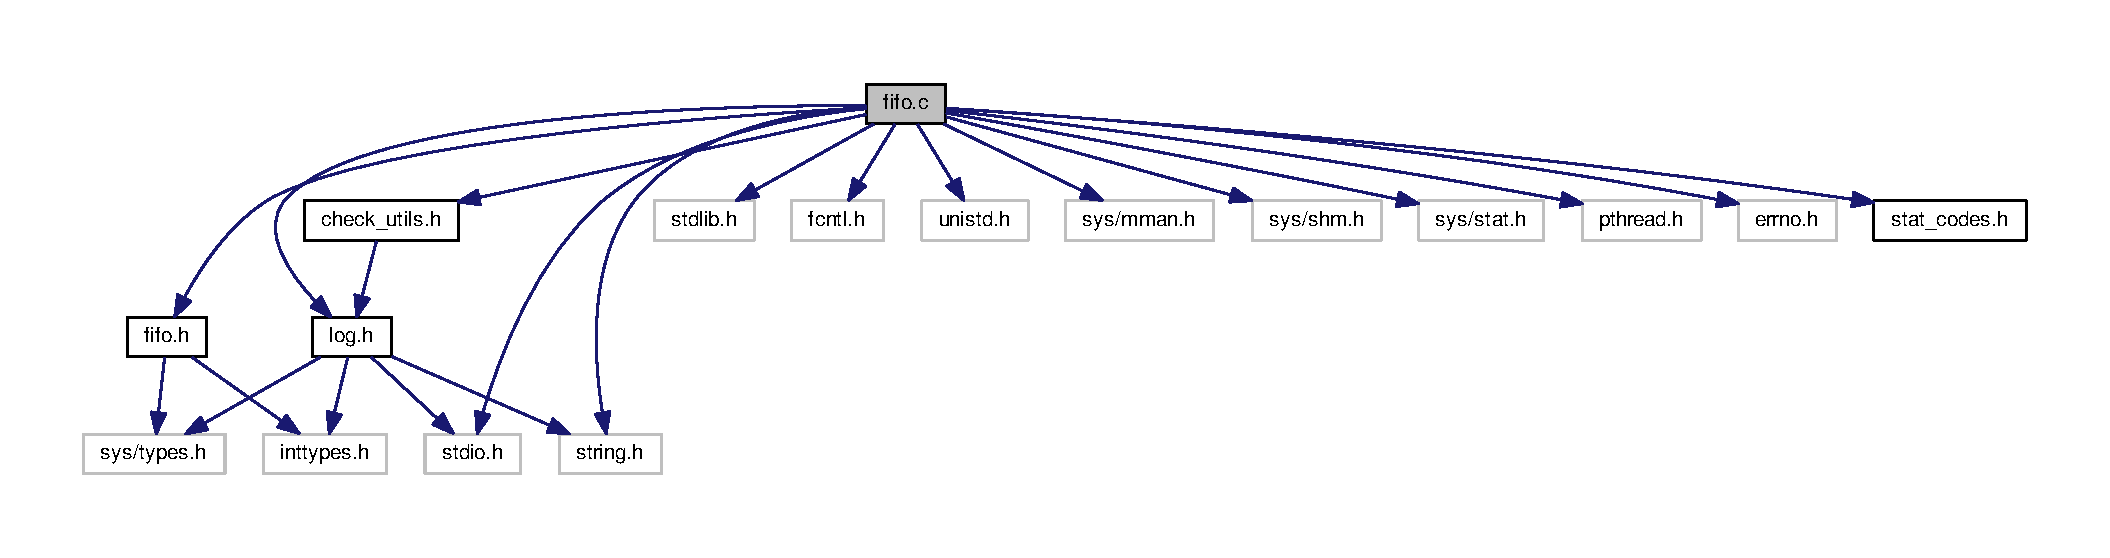
\includegraphics[width=350pt]{fifo_8c__incl}
\end{center}
\end{figure}
\subsection*{Classes}
\begin{DoxyCompactItemize}
\item 
struct \hyperlink{structfifo__elem__ctx__s}{fifo\+\_\+elem\+\_\+ctx\+\_\+s}
\item 
struct \hyperlink{structfifo__ctx__s}{fifo\+\_\+ctx\+\_\+s}
\end{DoxyCompactItemize}
\subsection*{Macros}
\begin{DoxyCompactItemize}
\item 
\#define \hyperlink{fifo_8c_afe4ee3f0e7e613d79afb3ccb9e552c0d}{S\+I\+Z\+E\+O\+F\+\_\+\+F\+I\+F\+O\+\_\+\+E\+L\+E\+M\+\_\+\+C\+T\+X\+\_\+T}(F\+L\+A\+G\+\_\+\+U\+S\+E\+\_\+\+S\+HM,  C\+H\+U\+N\+K\+\_\+\+S\+I\+Z\+E\+\_\+\+M\+AX)~(size\+\_\+t)(sizeof(\hyperlink{fifo_8c_a3236a0200db719fdeb6d875a415ca7c9}{fifo\+\_\+elem\+\_\+ctx\+\_\+t})+ (F\+L\+A\+G\+\_\+\+U\+S\+E\+\_\+\+S\+HM== 0? 1\+: C\+H\+U\+N\+K\+\_\+\+S\+I\+Z\+E\+\_\+\+M\+AX))
\item 
\#define \hyperlink{fifo_8c_a42708bf618db9ea973b091a2d5bdfa9e}{F\+I\+F\+O\+\_\+\+F\+I\+L\+E\+\_\+\+N\+A\+M\+E\+\_\+\+M\+A\+X\+\_\+\+S\+I\+ZE}~1024
\end{DoxyCompactItemize}
\subsection*{Typedefs}
\begin{DoxyCompactItemize}
\item 
typedef struct \hyperlink{structfifo__elem__ctx__s}{fifo\+\_\+elem\+\_\+ctx\+\_\+s} \hyperlink{fifo_8c_a3236a0200db719fdeb6d875a415ca7c9}{fifo\+\_\+elem\+\_\+ctx\+\_\+t}
\item 
typedef struct \hyperlink{structfifo__ctx__s}{fifo\+\_\+ctx\+\_\+s} \hyperlink{fifo_8c_acf3f21e64cbabccd8420c306740820c1}{fifo\+\_\+ctx\+\_\+t}
\end{DoxyCompactItemize}
\subsection*{Functions}
\begin{DoxyCompactItemize}
\item 
static void \hyperlink{fifo_8c_a653d3763790d5f750f801b886b4b6c64}{fifo\+\_\+close\+\_\+internal} (\hyperlink{fifo_8c_acf3f21e64cbabccd8420c306740820c1}{fifo\+\_\+ctx\+\_\+t} $\ast$$\ast$ref\+\_\+fifo\+\_\+ctx, int flag\+\_\+deinit)
\item 
static int \hyperlink{fifo_8c_a2dcffabb4232225fed4b8a1805719288}{fifo\+\_\+init} (\hyperlink{fifo_8c_acf3f21e64cbabccd8420c306740820c1}{fifo\+\_\+ctx\+\_\+t} $\ast$fifo\+\_\+ctx, size\+\_\+t slots\+\_\+max, size\+\_\+t chunk\+\_\+size\+\_\+max, uint32\+\_\+t flags, const char $\ast$fifo\+\_\+file\+\_\+name, const \hyperlink{structfifo__elem__alloc__fxn__s}{fifo\+\_\+elem\+\_\+alloc\+\_\+fxn\+\_\+t} $\ast$fifo\+\_\+elem\+\_\+alloc\+\_\+fxn)
\item 
static void \hyperlink{fifo_8c_a6573ac4da0bc7e4ab51e2433beba806b}{fifo\+\_\+deinit} (\hyperlink{fifo_8c_acf3f21e64cbabccd8420c306740820c1}{fifo\+\_\+ctx\+\_\+t} $\ast$fifo\+\_\+ctx)
\item 
static int {\bfseries fifo\+\_\+input} (\hyperlink{fifo_8c_acf3f21e64cbabccd8420c306740820c1}{fifo\+\_\+ctx\+\_\+t} $\ast$fifo\+\_\+ctx, void $\ast$$\ast$ref\+\_\+elem, size\+\_\+t elem\+\_\+size, int dup\+\_\+flag)\hypertarget{fifo_8c_afcb545f297176708c0d59ee27aa83e07}{}\label{fifo_8c_afcb545f297176708c0d59ee27aa83e07}

\item 
static int {\bfseries fifo\+\_\+output} (\hyperlink{fifo_8c_acf3f21e64cbabccd8420c306740820c1}{fifo\+\_\+ctx\+\_\+t} $\ast$fifo\+\_\+ctx, void $\ast$$\ast$ref\+\_\+elem, size\+\_\+t $\ast$ref\+\_\+elem\+\_\+size, int flush\+\_\+flag, int64\+\_\+t tout\+\_\+usecs)\hypertarget{fifo_8c_aa9de23c47bfe7b8478be73f732911854}{}\label{fifo_8c_aa9de23c47bfe7b8478be73f732911854}

\item 
static int {\bfseries fifo\+\_\+mutex\+\_\+init} (pthread\+\_\+mutex\+\_\+t $\ast$const pthread\+\_\+mutex\+\_\+p, int flag\+\_\+use\+\_\+shm, \hyperlink{structlog__ctx__s}{log\+\_\+ctx\+\_\+t} $\ast$log\+\_\+ctx)\hypertarget{fifo_8c_a5bdd78cdbb33b01fb34dae50120017c6}{}\label{fifo_8c_a5bdd78cdbb33b01fb34dae50120017c6}

\item 
static int {\bfseries fifo\+\_\+cond\+\_\+init} (pthread\+\_\+cond\+\_\+t $\ast$const pthread\+\_\+cond\+\_\+p, int flag\+\_\+use\+\_\+shm, \hyperlink{structlog__ctx__s}{log\+\_\+ctx\+\_\+t} $\ast$log\+\_\+ctx)\hypertarget{fifo_8c_af316d8192b5beffa9b3d2e565255f4fc}{}\label{fifo_8c_af316d8192b5beffa9b3d2e565255f4fc}

\item 
\hyperlink{fifo_8c_acf3f21e64cbabccd8420c306740820c1}{fifo\+\_\+ctx\+\_\+t} $\ast$ \hyperlink{fifo_8c_a06a3217e8cb0f8976fa7632effed3220}{fifo\+\_\+open} (size\+\_\+t slots\+\_\+max, size\+\_\+t chunk\+\_\+size\+\_\+max, uint32\+\_\+t flags, const \hyperlink{structfifo__elem__alloc__fxn__s}{fifo\+\_\+elem\+\_\+alloc\+\_\+fxn\+\_\+t} $\ast$fifo\+\_\+elem\+\_\+alloc\+\_\+fxn)
\item 
\hyperlink{fifo_8c_acf3f21e64cbabccd8420c306740820c1}{fifo\+\_\+ctx\+\_\+t} $\ast$ \hyperlink{fifo_8c_aa6eed5bf3f4cadd29fae7e9fe83aed12}{fifo\+\_\+shm\+\_\+open} (size\+\_\+t slots\+\_\+max, size\+\_\+t chunk\+\_\+size\+\_\+max, uint32\+\_\+t flags, const char $\ast$fifo\+\_\+file\+\_\+name)
\item 
\hyperlink{fifo_8c_acf3f21e64cbabccd8420c306740820c1}{fifo\+\_\+ctx\+\_\+t} $\ast$ {\bfseries fifo\+\_\+shm\+\_\+exec\+\_\+open} (size\+\_\+t slots\+\_\+max, size\+\_\+t chunk\+\_\+size\+\_\+max, uint32\+\_\+t flags, const char $\ast$fifo\+\_\+file\+\_\+name)\hypertarget{fifo_8c_a7cc850453cad4cb1bfb879f1c088c828}{}\label{fifo_8c_a7cc850453cad4cb1bfb879f1c088c828}

\item 
void \hyperlink{fifo_8c_a0b7d820309ccf81a3b39bc7984c7697a}{fifo\+\_\+close} (\hyperlink{fifo_8c_acf3f21e64cbabccd8420c306740820c1}{fifo\+\_\+ctx\+\_\+t} $\ast$$\ast$ref\+\_\+fifo\+\_\+ctx)
\item 
void \hyperlink{fifo_8c_a2611719de8a50e56a040036114de9e88}{fifo\+\_\+set\+\_\+blocking\+\_\+mode} (\hyperlink{fifo_8c_acf3f21e64cbabccd8420c306740820c1}{fifo\+\_\+ctx\+\_\+t} $\ast$fifo\+\_\+ctx, int do\+\_\+block)
\item 
int \hyperlink{fifo_8c_ae01dccc89399239175f99002572151e0}{fifo\+\_\+put\+\_\+dup} (\hyperlink{fifo_8c_acf3f21e64cbabccd8420c306740820c1}{fifo\+\_\+ctx\+\_\+t} $\ast$fifo\+\_\+ctx, const void $\ast$elem, size\+\_\+t elem\+\_\+size)
\item 
int \hyperlink{fifo_8c_a2fe81cc19210968f18f23493a35b6a49}{fifo\+\_\+put} (\hyperlink{fifo_8c_acf3f21e64cbabccd8420c306740820c1}{fifo\+\_\+ctx\+\_\+t} $\ast$fifo\+\_\+ctx, void $\ast$$\ast$ref\+\_\+elem, size\+\_\+t elem\+\_\+size)
\item 
int \hyperlink{fifo_8c_a85a5e85ab81f3a1ea3464ff57fcf8f88}{fifo\+\_\+get} (\hyperlink{fifo_8c_acf3f21e64cbabccd8420c306740820c1}{fifo\+\_\+ctx\+\_\+t} $\ast$fifo\+\_\+ctx, void $\ast$$\ast$ref\+\_\+elem, size\+\_\+t $\ast$ref\+\_\+elem\+\_\+size)
\item 
int \hyperlink{fifo_8c_a277fe27d1a899d61e7b1e838ffe1c784}{fifo\+\_\+timedget} (\hyperlink{fifo_8c_acf3f21e64cbabccd8420c306740820c1}{fifo\+\_\+ctx\+\_\+t} $\ast$fifo\+\_\+ctx, void $\ast$$\ast$ref\+\_\+elem, size\+\_\+t $\ast$ref\+\_\+elem\+\_\+size, int64\+\_\+t tout\+\_\+usecs)
\item 
int \hyperlink{fifo_8c_aef3f90505f9d094700f99064aee174da}{fifo\+\_\+show} (\hyperlink{fifo_8c_acf3f21e64cbabccd8420c306740820c1}{fifo\+\_\+ctx\+\_\+t} $\ast$fifo\+\_\+ctx, void $\ast$$\ast$ref\+\_\+elem, size\+\_\+t $\ast$ref\+\_\+elem\+\_\+size)
\item 
ssize\+\_\+t \hyperlink{fifo_8c_ad11b8d4bba268df196ddd3b3a8df3033}{fifo\+\_\+get\+\_\+buffer\+\_\+level} (\hyperlink{fifo_8c_acf3f21e64cbabccd8420c306740820c1}{fifo\+\_\+ctx\+\_\+t} $\ast$fifo\+\_\+ctx)
\item 
int \hyperlink{fifo_8c_acebb289956cc3f7254d0e8bb5b6ca38a}{fifo\+\_\+traverse} (\hyperlink{fifo_8c_acf3f21e64cbabccd8420c306740820c1}{fifo\+\_\+ctx\+\_\+t} $\ast$fifo\+\_\+ctx, int elem\+\_\+cnt, void($\ast$it\+\_\+fxn)(void $\ast$elem, ssize\+\_\+t elem\+\_\+size, int idx, void $\ast$it\+\_\+arg, int $\ast$ref\+\_\+flag\+\_\+break), void $\ast$it\+\_\+arg)
\item 
void \hyperlink{fifo_8c_a2c0c91155b8d071ae30a07fa866372bc}{fifo\+\_\+empty} (\hyperlink{fifo_8c_acf3f21e64cbabccd8420c306740820c1}{fifo\+\_\+ctx\+\_\+t} $\ast$fifo\+\_\+ctx)
\end{DoxyCompactItemize}


\subsection{Detailed Description}
\begin{DoxyAuthor}{Author}
Rafael Antoniello 
\end{DoxyAuthor}


\subsection{Macro Definition Documentation}
\index{fifo.\+c@{fifo.\+c}!F\+I\+F\+O\+\_\+\+F\+I\+L\+E\+\_\+\+N\+A\+M\+E\+\_\+\+M\+A\+X\+\_\+\+S\+I\+ZE@{F\+I\+F\+O\+\_\+\+F\+I\+L\+E\+\_\+\+N\+A\+M\+E\+\_\+\+M\+A\+X\+\_\+\+S\+I\+ZE}}
\index{F\+I\+F\+O\+\_\+\+F\+I\+L\+E\+\_\+\+N\+A\+M\+E\+\_\+\+M\+A\+X\+\_\+\+S\+I\+ZE@{F\+I\+F\+O\+\_\+\+F\+I\+L\+E\+\_\+\+N\+A\+M\+E\+\_\+\+M\+A\+X\+\_\+\+S\+I\+ZE}!fifo.\+c@{fifo.\+c}}
\subsubsection[{\texorpdfstring{F\+I\+F\+O\+\_\+\+F\+I\+L\+E\+\_\+\+N\+A\+M\+E\+\_\+\+M\+A\+X\+\_\+\+S\+I\+ZE}{FIFO_FILE_NAME_MAX_SIZE}}]{\setlength{\rightskip}{0pt plus 5cm}\#define F\+I\+F\+O\+\_\+\+F\+I\+L\+E\+\_\+\+N\+A\+M\+E\+\_\+\+M\+A\+X\+\_\+\+S\+I\+ZE~1024}\hypertarget{fifo_8c_a42708bf618db9ea973b091a2d5bdfa9e}{}\label{fifo_8c_a42708bf618db9ea973b091a2d5bdfa9e}
Used only if F\+I\+F\+O\+\_\+\+P\+R\+O\+C\+E\+S\+S\+\_\+\+S\+H\+A\+R\+ED is signaled. In this case, this file-\/name is assigned to the shared memory object to facilitate opening F\+I\+FO from an fork-\/exec setting. 

Definition at line 104 of file fifo.\+c.

\index{fifo.\+c@{fifo.\+c}!S\+I\+Z\+E\+O\+F\+\_\+\+F\+I\+F\+O\+\_\+\+E\+L\+E\+M\+\_\+\+C\+T\+X\+\_\+T@{S\+I\+Z\+E\+O\+F\+\_\+\+F\+I\+F\+O\+\_\+\+E\+L\+E\+M\+\_\+\+C\+T\+X\+\_\+T}}
\index{S\+I\+Z\+E\+O\+F\+\_\+\+F\+I\+F\+O\+\_\+\+E\+L\+E\+M\+\_\+\+C\+T\+X\+\_\+T@{S\+I\+Z\+E\+O\+F\+\_\+\+F\+I\+F\+O\+\_\+\+E\+L\+E\+M\+\_\+\+C\+T\+X\+\_\+T}!fifo.\+c@{fifo.\+c}}
\subsubsection[{\texorpdfstring{S\+I\+Z\+E\+O\+F\+\_\+\+F\+I\+F\+O\+\_\+\+E\+L\+E\+M\+\_\+\+C\+T\+X\+\_\+T}{SIZEOF_FIFO_ELEM_CTX_T}}]{\setlength{\rightskip}{0pt plus 5cm}\#define S\+I\+Z\+E\+O\+F\+\_\+\+F\+I\+F\+O\+\_\+\+E\+L\+E\+M\+\_\+\+C\+T\+X\+\_\+T(
\begin{DoxyParamCaption}
\item[{}]{F\+L\+A\+G\+\_\+\+U\+S\+E\+\_\+\+S\+HM, }
\item[{}]{C\+H\+U\+N\+K\+\_\+\+S\+I\+Z\+E\+\_\+\+M\+AX}
\end{DoxyParamCaption}
)~(size\+\_\+t)(sizeof({\bf fifo\+\_\+elem\+\_\+ctx\+\_\+t})+ (F\+L\+A\+G\+\_\+\+U\+S\+E\+\_\+\+S\+HM== 0? 1\+: C\+H\+U\+N\+K\+\_\+\+S\+I\+Z\+E\+\_\+\+M\+AX))}\hypertarget{fifo_8c_afe4ee3f0e7e613d79afb3ccb9e552c0d}{}\label{fifo_8c_afe4ee3f0e7e613d79afb3ccb9e552c0d}
Size of structure type \textquotesingle{}fifo\+\_\+elem\+\_\+ctx\+\_\+t\textquotesingle{}. In the case F\+L\+A\+G\+\_\+\+U\+S\+E\+\_\+\+S\+HM flag is set, \hyperlink{structfifo__elem__ctx__s_a77ec4386ce2ca348e6d9c9ced4fafa92}{fifo\+\_\+elem\+\_\+ctx\+\_\+t\+::shm\+\_\+elem\+\_\+pool} will be actually a predefined buffer with a maximum fixed size of \textquotesingle{}C\+H\+U\+N\+K\+\_\+\+S\+I\+Z\+E\+\_\+\+M\+AX\textquotesingle{} octets. Otherwise, member \hyperlink{structfifo__elem__ctx__s_a77ec4386ce2ca348e6d9c9ced4fafa92}{fifo\+\_\+elem\+\_\+ctx\+\_\+t\+::shm\+\_\+elem\+\_\+pool} will not be used (giving a minimum legacy size). 

Definition at line 61 of file fifo.\+c.



\subsection{Typedef Documentation}
\index{fifo.\+c@{fifo.\+c}!fifo\+\_\+ctx\+\_\+t@{fifo\+\_\+ctx\+\_\+t}}
\index{fifo\+\_\+ctx\+\_\+t@{fifo\+\_\+ctx\+\_\+t}!fifo.\+c@{fifo.\+c}}
\subsubsection[{\texorpdfstring{fifo\+\_\+ctx\+\_\+t}{fifo_ctx_t}}]{\setlength{\rightskip}{0pt plus 5cm}typedef struct {\bf fifo\+\_\+ctx\+\_\+s}  {\bf fifo\+\_\+ctx\+\_\+t}}\hypertarget{fifo_8c_acf3f21e64cbabccd8420c306740820c1}{}\label{fifo_8c_acf3f21e64cbabccd8420c306740820c1}
F\+I\+FO context structure. \index{fifo.\+c@{fifo.\+c}!fifo\+\_\+elem\+\_\+ctx\+\_\+t@{fifo\+\_\+elem\+\_\+ctx\+\_\+t}}
\index{fifo\+\_\+elem\+\_\+ctx\+\_\+t@{fifo\+\_\+elem\+\_\+ctx\+\_\+t}!fifo.\+c@{fifo.\+c}}
\subsubsection[{\texorpdfstring{fifo\+\_\+elem\+\_\+ctx\+\_\+t}{fifo_elem_ctx_t}}]{\setlength{\rightskip}{0pt plus 5cm}typedef struct {\bf fifo\+\_\+elem\+\_\+ctx\+\_\+s}  {\bf fifo\+\_\+elem\+\_\+ctx\+\_\+t}}\hypertarget{fifo_8c_a3236a0200db719fdeb6d875a415ca7c9}{}\label{fifo_8c_a3236a0200db719fdeb6d875a415ca7c9}
F\+I\+FO element context structure. 

\subsection{Function Documentation}
\index{fifo.\+c@{fifo.\+c}!fifo\+\_\+close@{fifo\+\_\+close}}
\index{fifo\+\_\+close@{fifo\+\_\+close}!fifo.\+c@{fifo.\+c}}
\subsubsection[{\texorpdfstring{fifo\+\_\+close(fifo\+\_\+ctx\+\_\+t $\ast$$\ast$ref\+\_\+fifo\+\_\+ctx)}{fifo_close(fifo_ctx_t **ref_fifo_ctx)}}]{\setlength{\rightskip}{0pt plus 5cm}void fifo\+\_\+close (
\begin{DoxyParamCaption}
\item[{{\bf fifo\+\_\+ctx\+\_\+t} $\ast$$\ast$}]{ref\+\_\+fifo\+\_\+ctx}
\end{DoxyParamCaption}
)}\hypertarget{fifo_8c_a0b7d820309ccf81a3b39bc7984c7697a}{}\label{fifo_8c_a0b7d820309ccf81a3b39bc7984c7697a}
//\+T\+O\+DO 

Definition at line 327 of file fifo.\+c.

\index{fifo.\+c@{fifo.\+c}!fifo\+\_\+close\+\_\+internal@{fifo\+\_\+close\+\_\+internal}}
\index{fifo\+\_\+close\+\_\+internal@{fifo\+\_\+close\+\_\+internal}!fifo.\+c@{fifo.\+c}}
\subsubsection[{\texorpdfstring{fifo\+\_\+close\+\_\+internal(fifo\+\_\+ctx\+\_\+t $\ast$$\ast$ref\+\_\+fifo\+\_\+ctx, int flag\+\_\+deinit)}{fifo_close_internal(fifo_ctx_t **ref_fifo_ctx, int flag_deinit)}}]{\setlength{\rightskip}{0pt plus 5cm}static void fifo\+\_\+close\+\_\+internal (
\begin{DoxyParamCaption}
\item[{{\bf fifo\+\_\+ctx\+\_\+t} $\ast$$\ast$}]{ref\+\_\+fifo\+\_\+ctx, }
\item[{int}]{flag\+\_\+deinit}
\end{DoxyParamCaption}
)\hspace{0.3cm}{\ttfamily [static]}}\hypertarget{fifo_8c_a653d3763790d5f750f801b886b4b6c64}{}\label{fifo_8c_a653d3763790d5f750f801b886b4b6c64}
Internal F\+I\+FO closing function. Only parent process (not child) should de-\/initialize F\+I\+FO while closing. 
\begin{DoxyParams}{Parameters}
{\em ref\+\_\+fifo\+\_\+ctx} & \\
\hline
{\em flag\+\_\+deinit} & \\
\hline
\end{DoxyParams}


Definition at line 508 of file fifo.\+c.

\index{fifo.\+c@{fifo.\+c}!fifo\+\_\+deinit@{fifo\+\_\+deinit}}
\index{fifo\+\_\+deinit@{fifo\+\_\+deinit}!fifo.\+c@{fifo.\+c}}
\subsubsection[{\texorpdfstring{fifo\+\_\+deinit(fifo\+\_\+ctx\+\_\+t $\ast$fifo\+\_\+ctx)}{fifo_deinit(fifo_ctx_t *fifo_ctx)}}]{\setlength{\rightskip}{0pt plus 5cm}static void fifo\+\_\+deinit (
\begin{DoxyParamCaption}
\item[{{\bf fifo\+\_\+ctx\+\_\+t} $\ast$}]{fifo\+\_\+ctx}
\end{DoxyParamCaption}
)\hspace{0.3cm}{\ttfamily [static]}}\hypertarget{fifo_8c_a6573ac4da0bc7e4ab51e2433beba806b}{}\label{fifo_8c_a6573ac4da0bc7e4ab51e2433beba806b}
De-\/initialize F\+I\+FO context structure. 
\begin{DoxyParams}{Parameters}
{\em fifo\+\_\+ctx} & \\
\hline
\end{DoxyParams}


Definition at line 636 of file fifo.\+c.

\index{fifo.\+c@{fifo.\+c}!fifo\+\_\+empty@{fifo\+\_\+empty}}
\index{fifo\+\_\+empty@{fifo\+\_\+empty}!fifo.\+c@{fifo.\+c}}
\subsubsection[{\texorpdfstring{fifo\+\_\+empty(fifo\+\_\+ctx\+\_\+t $\ast$fifo\+\_\+ctx)}{fifo_empty(fifo_ctx_t *fifo_ctx)}}]{\setlength{\rightskip}{0pt plus 5cm}void fifo\+\_\+empty (
\begin{DoxyParamCaption}
\item[{{\bf fifo\+\_\+ctx\+\_\+t} $\ast$}]{fifo\+\_\+ctx}
\end{DoxyParamCaption}
)}\hypertarget{fifo_8c_a2c0c91155b8d071ae30a07fa866372bc}{}\label{fifo_8c_a2c0c91155b8d071ae30a07fa866372bc}
//\+T\+O\+DO 

Definition at line 456 of file fifo.\+c.

\index{fifo.\+c@{fifo.\+c}!fifo\+\_\+get@{fifo\+\_\+get}}
\index{fifo\+\_\+get@{fifo\+\_\+get}!fifo.\+c@{fifo.\+c}}
\subsubsection[{\texorpdfstring{fifo\+\_\+get(fifo\+\_\+ctx\+\_\+t $\ast$fifo\+\_\+ctx, void $\ast$$\ast$ref\+\_\+elem, size\+\_\+t $\ast$ref\+\_\+elem\+\_\+size)}{fifo_get(fifo_ctx_t *fifo_ctx, void **ref_elem, size_t *ref_elem_size)}}]{\setlength{\rightskip}{0pt plus 5cm}int fifo\+\_\+get (
\begin{DoxyParamCaption}
\item[{{\bf fifo\+\_\+ctx\+\_\+t} $\ast$}]{fifo\+\_\+ctx, }
\item[{void $\ast$$\ast$}]{ref\+\_\+elem, }
\item[{size\+\_\+t $\ast$}]{ref\+\_\+elem\+\_\+size}
\end{DoxyParamCaption}
)}\hypertarget{fifo_8c_a85a5e85ab81f3a1ea3464ff57fcf8f88}{}\label{fifo_8c_a85a5e85ab81f3a1ea3464ff57fcf8f88}
//\+T\+O\+DO 

Definition at line 366 of file fifo.\+c.

\index{fifo.\+c@{fifo.\+c}!fifo\+\_\+get\+\_\+buffer\+\_\+level@{fifo\+\_\+get\+\_\+buffer\+\_\+level}}
\index{fifo\+\_\+get\+\_\+buffer\+\_\+level@{fifo\+\_\+get\+\_\+buffer\+\_\+level}!fifo.\+c@{fifo.\+c}}
\subsubsection[{\texorpdfstring{fifo\+\_\+get\+\_\+buffer\+\_\+level(fifo\+\_\+ctx\+\_\+t $\ast$fifo\+\_\+ctx)}{fifo_get_buffer_level(fifo_ctx_t *fifo_ctx)}}]{\setlength{\rightskip}{0pt plus 5cm}ssize\+\_\+t fifo\+\_\+get\+\_\+buffer\+\_\+level (
\begin{DoxyParamCaption}
\item[{{\bf fifo\+\_\+ctx\+\_\+t} $\ast$}]{fifo\+\_\+ctx}
\end{DoxyParamCaption}
)}\hypertarget{fifo_8c_ad11b8d4bba268df196ddd3b3a8df3033}{}\label{fifo_8c_ad11b8d4bba268df196ddd3b3a8df3033}
//\+T\+O\+DO 

Definition at line 385 of file fifo.\+c.

\index{fifo.\+c@{fifo.\+c}!fifo\+\_\+init@{fifo\+\_\+init}}
\index{fifo\+\_\+init@{fifo\+\_\+init}!fifo.\+c@{fifo.\+c}}
\subsubsection[{\texorpdfstring{fifo\+\_\+init(fifo\+\_\+ctx\+\_\+t $\ast$fifo\+\_\+ctx, size\+\_\+t slots\+\_\+max, size\+\_\+t chunk\+\_\+size\+\_\+max, uint32\+\_\+t flags, const char $\ast$fifo\+\_\+file\+\_\+name, const fifo\+\_\+elem\+\_\+alloc\+\_\+fxn\+\_\+t $\ast$fifo\+\_\+elem\+\_\+alloc\+\_\+fxn)}{fifo_init(fifo_ctx_t *fifo_ctx, size_t slots_max, size_t chunk_size_max, uint32_t flags, const char *fifo_file_name, const fifo_elem_alloc_fxn_t *fifo_elem_alloc_fxn)}}]{\setlength{\rightskip}{0pt plus 5cm}static int fifo\+\_\+init (
\begin{DoxyParamCaption}
\item[{{\bf fifo\+\_\+ctx\+\_\+t} $\ast$}]{fifo\+\_\+ctx, }
\item[{size\+\_\+t}]{slots\+\_\+max, }
\item[{size\+\_\+t}]{chunk\+\_\+size\+\_\+max, }
\item[{uint32\+\_\+t}]{flags, }
\item[{const char $\ast$}]{fifo\+\_\+file\+\_\+name, }
\item[{const {\bf fifo\+\_\+elem\+\_\+alloc\+\_\+fxn\+\_\+t} $\ast$}]{fifo\+\_\+elem\+\_\+alloc\+\_\+fxn}
\end{DoxyParamCaption}
)\hspace{0.3cm}{\ttfamily [static]}}\hypertarget{fifo_8c_a2dcffabb4232225fed4b8a1805719288}{}\label{fifo_8c_a2dcffabb4232225fed4b8a1805719288}
Initialize F\+I\+FO context structure. 
\begin{DoxyParams}{Parameters}
{\em fifo\+\_\+ctx} & \\
\hline
\end{DoxyParams}
\begin{DoxyReturn}{Returns}
Status code (refer to \textquotesingle{}stat\+\_\+codes\+\_\+ctx\+\_\+t\textquotesingle{} type). 
\end{DoxyReturn}


Definition at line 538 of file fifo.\+c.

\index{fifo.\+c@{fifo.\+c}!fifo\+\_\+open@{fifo\+\_\+open}}
\index{fifo\+\_\+open@{fifo\+\_\+open}!fifo.\+c@{fifo.\+c}}
\subsubsection[{\texorpdfstring{fifo\+\_\+open(size\+\_\+t slots\+\_\+max, size\+\_\+t chunk\+\_\+size\+\_\+max, uint32\+\_\+t flags, const fifo\+\_\+elem\+\_\+alloc\+\_\+fxn\+\_\+t $\ast$fifo\+\_\+elem\+\_\+alloc\+\_\+fxn)}{fifo_open(size_t slots_max, size_t chunk_size_max, uint32_t flags, const fifo_elem_alloc_fxn_t *fifo_elem_alloc_fxn)}}]{\setlength{\rightskip}{0pt plus 5cm}{\bf fifo\+\_\+ctx\+\_\+t}$\ast$ fifo\+\_\+open (
\begin{DoxyParamCaption}
\item[{size\+\_\+t}]{slots\+\_\+max, }
\item[{size\+\_\+t}]{chunk\+\_\+size\+\_\+max, }
\item[{uint32\+\_\+t}]{flags, }
\item[{const {\bf fifo\+\_\+elem\+\_\+alloc\+\_\+fxn\+\_\+t} $\ast$}]{fifo\+\_\+elem\+\_\+alloc\+\_\+fxn}
\end{DoxyParamCaption}
)}\hypertarget{fifo_8c_a06a3217e8cb0f8976fa7632effed3220}{}\label{fifo_8c_a06a3217e8cb0f8976fa7632effed3220}
//\+T\+O\+DO 

Definition at line 195 of file fifo.\+c.

\index{fifo.\+c@{fifo.\+c}!fifo\+\_\+put@{fifo\+\_\+put}}
\index{fifo\+\_\+put@{fifo\+\_\+put}!fifo.\+c@{fifo.\+c}}
\subsubsection[{\texorpdfstring{fifo\+\_\+put(fifo\+\_\+ctx\+\_\+t $\ast$fifo\+\_\+ctx, void $\ast$$\ast$ref\+\_\+elem, size\+\_\+t elem\+\_\+size)}{fifo_put(fifo_ctx_t *fifo_ctx, void **ref_elem, size_t elem_size)}}]{\setlength{\rightskip}{0pt plus 5cm}int fifo\+\_\+put (
\begin{DoxyParamCaption}
\item[{{\bf fifo\+\_\+ctx\+\_\+t} $\ast$}]{fifo\+\_\+ctx, }
\item[{void $\ast$$\ast$}]{ref\+\_\+elem, }
\item[{size\+\_\+t}]{elem\+\_\+size}
\end{DoxyParamCaption}
)}\hypertarget{fifo_8c_a2fe81cc19210968f18f23493a35b6a49}{}\label{fifo_8c_a2fe81cc19210968f18f23493a35b6a49}
//\+T\+O\+DO 

Definition at line 361 of file fifo.\+c.

\index{fifo.\+c@{fifo.\+c}!fifo\+\_\+put\+\_\+dup@{fifo\+\_\+put\+\_\+dup}}
\index{fifo\+\_\+put\+\_\+dup@{fifo\+\_\+put\+\_\+dup}!fifo.\+c@{fifo.\+c}}
\subsubsection[{\texorpdfstring{fifo\+\_\+put\+\_\+dup(fifo\+\_\+ctx\+\_\+t $\ast$fifo\+\_\+ctx, const void $\ast$elem, size\+\_\+t elem\+\_\+size)}{fifo_put_dup(fifo_ctx_t *fifo_ctx, const void *elem, size_t elem_size)}}]{\setlength{\rightskip}{0pt plus 5cm}int fifo\+\_\+put\+\_\+dup (
\begin{DoxyParamCaption}
\item[{{\bf fifo\+\_\+ctx\+\_\+t} $\ast$}]{fifo\+\_\+ctx, }
\item[{const void $\ast$}]{elem, }
\item[{size\+\_\+t}]{elem\+\_\+size}
\end{DoxyParamCaption}
)}\hypertarget{fifo_8c_ae01dccc89399239175f99002572151e0}{}\label{fifo_8c_ae01dccc89399239175f99002572151e0}
//\+T\+O\+DO 

Definition at line 355 of file fifo.\+c.

\index{fifo.\+c@{fifo.\+c}!fifo\+\_\+set\+\_\+blocking\+\_\+mode@{fifo\+\_\+set\+\_\+blocking\+\_\+mode}}
\index{fifo\+\_\+set\+\_\+blocking\+\_\+mode@{fifo\+\_\+set\+\_\+blocking\+\_\+mode}!fifo.\+c@{fifo.\+c}}
\subsubsection[{\texorpdfstring{fifo\+\_\+set\+\_\+blocking\+\_\+mode(fifo\+\_\+ctx\+\_\+t $\ast$fifo\+\_\+ctx, int do\+\_\+block)}{fifo_set_blocking_mode(fifo_ctx_t *fifo_ctx, int do_block)}}]{\setlength{\rightskip}{0pt plus 5cm}void fifo\+\_\+set\+\_\+blocking\+\_\+mode (
\begin{DoxyParamCaption}
\item[{{\bf fifo\+\_\+ctx\+\_\+t} $\ast$}]{fifo\+\_\+ctx, }
\item[{int}]{do\+\_\+block}
\end{DoxyParamCaption}
)}\hypertarget{fifo_8c_a2611719de8a50e56a040036114de9e88}{}\label{fifo_8c_a2611719de8a50e56a040036114de9e88}
//\+T\+O\+DO 

Definition at line 332 of file fifo.\+c.

\index{fifo.\+c@{fifo.\+c}!fifo\+\_\+shm\+\_\+open@{fifo\+\_\+shm\+\_\+open}}
\index{fifo\+\_\+shm\+\_\+open@{fifo\+\_\+shm\+\_\+open}!fifo.\+c@{fifo.\+c}}
\subsubsection[{\texorpdfstring{fifo\+\_\+shm\+\_\+open(size\+\_\+t slots\+\_\+max, size\+\_\+t chunk\+\_\+size\+\_\+max, uint32\+\_\+t flags, const char $\ast$fifo\+\_\+file\+\_\+name)}{fifo_shm_open(size_t slots_max, size_t chunk_size_max, uint32_t flags, const char *fifo_file_name)}}]{\setlength{\rightskip}{0pt plus 5cm}{\bf fifo\+\_\+ctx\+\_\+t}$\ast$ fifo\+\_\+shm\+\_\+open (
\begin{DoxyParamCaption}
\item[{size\+\_\+t}]{slots\+\_\+max, }
\item[{size\+\_\+t}]{chunk\+\_\+size\+\_\+max, }
\item[{uint32\+\_\+t}]{flags, }
\item[{const char $\ast$}]{fifo\+\_\+file\+\_\+name}
\end{DoxyParamCaption}
)}\hypertarget{fifo_8c_aa6eed5bf3f4cadd29fae7e9fe83aed12}{}\label{fifo_8c_aa6eed5bf3f4cadd29fae7e9fe83aed12}

\begin{DoxyParams}{Parameters}
{\em slots\+\_\+max} & \\
\hline
{\em chunk\+\_\+size\+\_\+max} & \\
\hline
{\em flags} & \\
\hline
{\em fifo\+\_\+file\+\_\+name} & This file-\/name is assigned to the shared memory object to facilitate opening F\+I\+FO in a fork-\/exec setting. \\
\hline
\end{DoxyParams}


Definition at line 229 of file fifo.\+c.

\index{fifo.\+c@{fifo.\+c}!fifo\+\_\+show@{fifo\+\_\+show}}
\index{fifo\+\_\+show@{fifo\+\_\+show}!fifo.\+c@{fifo.\+c}}
\subsubsection[{\texorpdfstring{fifo\+\_\+show(fifo\+\_\+ctx\+\_\+t $\ast$fifo\+\_\+ctx, void $\ast$$\ast$ref\+\_\+elem, size\+\_\+t $\ast$ref\+\_\+elem\+\_\+size)}{fifo_show(fifo_ctx_t *fifo_ctx, void **ref_elem, size_t *ref_elem_size)}}]{\setlength{\rightskip}{0pt plus 5cm}int fifo\+\_\+show (
\begin{DoxyParamCaption}
\item[{{\bf fifo\+\_\+ctx\+\_\+t} $\ast$}]{fifo\+\_\+ctx, }
\item[{void $\ast$$\ast$}]{elem, }
\item[{size\+\_\+t $\ast$}]{elem\+\_\+size}
\end{DoxyParamCaption}
)}\hypertarget{fifo_8c_aef3f90505f9d094700f99064aee174da}{}\label{fifo_8c_aef3f90505f9d094700f99064aee174da}
//\+T\+O\+DO 

Definition at line 379 of file fifo.\+c.

\index{fifo.\+c@{fifo.\+c}!fifo\+\_\+timedget@{fifo\+\_\+timedget}}
\index{fifo\+\_\+timedget@{fifo\+\_\+timedget}!fifo.\+c@{fifo.\+c}}
\subsubsection[{\texorpdfstring{fifo\+\_\+timedget(fifo\+\_\+ctx\+\_\+t $\ast$fifo\+\_\+ctx, void $\ast$$\ast$ref\+\_\+elem, size\+\_\+t $\ast$ref\+\_\+elem\+\_\+size, int64\+\_\+t tout\+\_\+usecs)}{fifo_timedget(fifo_ctx_t *fifo_ctx, void **ref_elem, size_t *ref_elem_size, int64_t tout_usecs)}}]{\setlength{\rightskip}{0pt plus 5cm}int fifo\+\_\+timedget (
\begin{DoxyParamCaption}
\item[{{\bf fifo\+\_\+ctx\+\_\+t} $\ast$}]{fifo\+\_\+ctx, }
\item[{void $\ast$$\ast$}]{ref\+\_\+elem, }
\item[{size\+\_\+t $\ast$}]{ref\+\_\+elem\+\_\+size, }
\item[{int64\+\_\+t}]{tout\+\_\+usecs}
\end{DoxyParamCaption}
)}\hypertarget{fifo_8c_a277fe27d1a899d61e7b1e838ffe1c784}{}\label{fifo_8c_a277fe27d1a899d61e7b1e838ffe1c784}
//\+T\+O\+DO 

Definition at line 372 of file fifo.\+c.

\index{fifo.\+c@{fifo.\+c}!fifo\+\_\+traverse@{fifo\+\_\+traverse}}
\index{fifo\+\_\+traverse@{fifo\+\_\+traverse}!fifo.\+c@{fifo.\+c}}
\subsubsection[{\texorpdfstring{fifo\+\_\+traverse(fifo\+\_\+ctx\+\_\+t $\ast$fifo\+\_\+ctx, int elem\+\_\+cnt, void($\ast$it\+\_\+fxn)(void $\ast$elem, ssize\+\_\+t elem\+\_\+size, int idx, void $\ast$it\+\_\+arg, int $\ast$ref\+\_\+flag\+\_\+break), void $\ast$it\+\_\+arg)}{fifo_traverse(fifo_ctx_t *fifo_ctx, int elem_cnt, void(*it_fxn)(void *elem, ssize_t elem_size, int idx, void *it_arg, int *ref_flag_break), void *it_arg)}}]{\setlength{\rightskip}{0pt plus 5cm}int fifo\+\_\+traverse (
\begin{DoxyParamCaption}
\item[{{\bf fifo\+\_\+ctx\+\_\+t} $\ast$}]{fifo\+\_\+ctx, }
\item[{int}]{elem\+\_\+cnt, }
\item[{void($\ast$)(void $\ast$elem, ssize\+\_\+t elem\+\_\+size, int idx, void $\ast$it\+\_\+arg, int $\ast$ref\+\_\+flag\+\_\+break)}]{it\+\_\+fxn, }
\item[{void $\ast$}]{it\+\_\+arg}
\end{DoxyParamCaption}
)}\hypertarget{fifo_8c_acebb289956cc3f7254d0e8bb5b6ca38a}{}\label{fifo_8c_acebb289956cc3f7254d0e8bb5b6ca38a}
//\+T\+O\+DO 

Definition at line 400 of file fifo.\+c.


\hypertarget{fifo_8h}{}\section{fifo.\+h File Reference}
\label{fifo_8h}\index{fifo.\+h@{fifo.\+h}}


Simple pointer queue (F\+I\+FO) implementation.  


{\ttfamily \#include $<$sys/types.\+h$>$}\\*
{\ttfamily \#include $<$inttypes.\+h$>$}\\*
Include dependency graph for fifo.\+h\+:\nopagebreak
\begin{figure}[H]
\begin{center}
\leavevmode
\includegraphics[width=226pt]{fifo_8h__incl}
\end{center}
\end{figure}
This graph shows which files directly or indirectly include this file\+:\nopagebreak
\begin{figure}[H]
\begin{center}
\leavevmode
\includegraphics[width=118pt]{fifo_8h__dep__incl}
\end{center}
\end{figure}
\subsection*{Classes}
\begin{DoxyCompactItemize}
\item 
struct \hyperlink{structfifo__elem__alloc__fxn__s}{fifo\+\_\+elem\+\_\+alloc\+\_\+fxn\+\_\+s}
\end{DoxyCompactItemize}
\subsection*{Macros}
\begin{DoxyCompactItemize}
\item 
\#define \hyperlink{fifo_8h_a49519e161256d5a289e8280bc90cd9ef}{F\+I\+F\+O\+\_\+\+O\+\_\+\+N\+O\+N\+B\+L\+O\+CK}~1
\item 
\#define \hyperlink{fifo_8h_ae195cb592063cc829990078c608eb1b3}{F\+I\+F\+O\+\_\+\+P\+R\+O\+C\+E\+S\+S\+\_\+\+S\+H\+A\+R\+ED}~2
\end{DoxyCompactItemize}
\subsection*{Typedefs}
\begin{DoxyCompactItemize}
\item 
typedef struct \hyperlink{structfifo__ctx__s}{fifo\+\_\+ctx\+\_\+s} {\bfseries fifo\+\_\+ctx\+\_\+t}\hypertarget{fifo_8h_ac236baa51eea7e195ac745426ae30759}{}\label{fifo_8h_ac236baa51eea7e195ac745426ae30759}

\item 
typedef void $\ast$( {\bfseries fifo\+\_\+elem\+\_\+ctx\+\_\+dup\+\_\+fxn\+\_\+t}) (const void $\ast$)\hypertarget{fifo_8h_acca61df5fdf477f0d5461de16fede39c}{}\label{fifo_8h_acca61df5fdf477f0d5461de16fede39c}

\item 
typedef void( {\bfseries fifo\+\_\+elem\+\_\+ctx\+\_\+release\+\_\+fxn\+\_\+t}) (void $\ast$$\ast$)\hypertarget{fifo_8h_abda40d033dd5c5cf84992ac3d6be2dac}{}\label{fifo_8h_abda40d033dd5c5cf84992ac3d6be2dac}

\item 
typedef struct \hyperlink{structfifo__elem__alloc__fxn__s}{fifo\+\_\+elem\+\_\+alloc\+\_\+fxn\+\_\+s} {\bfseries fifo\+\_\+elem\+\_\+alloc\+\_\+fxn\+\_\+t}\hypertarget{fifo_8h_af1144de3246a569f6a9bc5a32c767054}{}\label{fifo_8h_af1144de3246a569f6a9bc5a32c767054}

\end{DoxyCompactItemize}
\subsection*{Functions}
\begin{DoxyCompactItemize}
\item 
\hyperlink{fifo_8c_acf3f21e64cbabccd8420c306740820c1}{fifo\+\_\+ctx\+\_\+t} $\ast$ \hyperlink{fifo_8h_a06a3217e8cb0f8976fa7632effed3220}{fifo\+\_\+open} (size\+\_\+t slots\+\_\+max, size\+\_\+t chunk\+\_\+size\+\_\+max, uint32\+\_\+t flags, const \hyperlink{structfifo__elem__alloc__fxn__s}{fifo\+\_\+elem\+\_\+alloc\+\_\+fxn\+\_\+t} $\ast$fifo\+\_\+elem\+\_\+alloc\+\_\+fxn)
\item 
\hyperlink{fifo_8c_acf3f21e64cbabccd8420c306740820c1}{fifo\+\_\+ctx\+\_\+t} $\ast$ \hyperlink{fifo_8h_aa6eed5bf3f4cadd29fae7e9fe83aed12}{fifo\+\_\+shm\+\_\+open} (size\+\_\+t slots\+\_\+max, size\+\_\+t chunk\+\_\+size\+\_\+max, uint32\+\_\+t flags, const char $\ast$fifo\+\_\+file\+\_\+name)
\item 
\hyperlink{fifo_8c_acf3f21e64cbabccd8420c306740820c1}{fifo\+\_\+ctx\+\_\+t} $\ast$ {\bfseries fifo\+\_\+shm\+\_\+exec\+\_\+open} (size\+\_\+t slots\+\_\+max, size\+\_\+t chunk\+\_\+size\+\_\+max, uint32\+\_\+t flags, const char $\ast$fifo\+\_\+file\+\_\+name)\hypertarget{fifo_8h_a7cc850453cad4cb1bfb879f1c088c828}{}\label{fifo_8h_a7cc850453cad4cb1bfb879f1c088c828}

\item 
void \hyperlink{fifo_8h_a0b7d820309ccf81a3b39bc7984c7697a}{fifo\+\_\+close} (\hyperlink{fifo_8c_acf3f21e64cbabccd8420c306740820c1}{fifo\+\_\+ctx\+\_\+t} $\ast$$\ast$ref\+\_\+fifo\+\_\+ctx)
\item 
void \hyperlink{fifo_8h_a2611719de8a50e56a040036114de9e88}{fifo\+\_\+set\+\_\+blocking\+\_\+mode} (\hyperlink{fifo_8c_acf3f21e64cbabccd8420c306740820c1}{fifo\+\_\+ctx\+\_\+t} $\ast$fifo\+\_\+ctx, int do\+\_\+block)
\item 
int \hyperlink{fifo_8h_ae01dccc89399239175f99002572151e0}{fifo\+\_\+put\+\_\+dup} (\hyperlink{fifo_8c_acf3f21e64cbabccd8420c306740820c1}{fifo\+\_\+ctx\+\_\+t} $\ast$fifo\+\_\+ctx, const void $\ast$elem, size\+\_\+t elem\+\_\+size)
\item 
int \hyperlink{fifo_8h_a2fe81cc19210968f18f23493a35b6a49}{fifo\+\_\+put} (\hyperlink{fifo_8c_acf3f21e64cbabccd8420c306740820c1}{fifo\+\_\+ctx\+\_\+t} $\ast$fifo\+\_\+ctx, void $\ast$$\ast$ref\+\_\+elem, size\+\_\+t elem\+\_\+size)
\item 
int \hyperlink{fifo_8h_a85a5e85ab81f3a1ea3464ff57fcf8f88}{fifo\+\_\+get} (\hyperlink{fifo_8c_acf3f21e64cbabccd8420c306740820c1}{fifo\+\_\+ctx\+\_\+t} $\ast$fifo\+\_\+ctx, void $\ast$$\ast$ref\+\_\+elem, size\+\_\+t $\ast$ref\+\_\+elem\+\_\+size)
\item 
int \hyperlink{fifo_8h_a277fe27d1a899d61e7b1e838ffe1c784}{fifo\+\_\+timedget} (\hyperlink{fifo_8c_acf3f21e64cbabccd8420c306740820c1}{fifo\+\_\+ctx\+\_\+t} $\ast$fifo\+\_\+ctx, void $\ast$$\ast$ref\+\_\+elem, size\+\_\+t $\ast$ref\+\_\+elem\+\_\+size, int64\+\_\+t tout\+\_\+usecs)
\item 
int \hyperlink{fifo_8h_a0793bad9ac8a0db8c1cd54a530a8e7ac}{fifo\+\_\+show} (\hyperlink{fifo_8c_acf3f21e64cbabccd8420c306740820c1}{fifo\+\_\+ctx\+\_\+t} $\ast$fifo\+\_\+ctx, void $\ast$$\ast$elem, size\+\_\+t $\ast$elem\+\_\+size)
\item 
ssize\+\_\+t \hyperlink{fifo_8h_ad11b8d4bba268df196ddd3b3a8df3033}{fifo\+\_\+get\+\_\+buffer\+\_\+level} (\hyperlink{fifo_8c_acf3f21e64cbabccd8420c306740820c1}{fifo\+\_\+ctx\+\_\+t} $\ast$fifo\+\_\+ctx)
\item 
int \hyperlink{fifo_8h_acebb289956cc3f7254d0e8bb5b6ca38a}{fifo\+\_\+traverse} (\hyperlink{fifo_8c_acf3f21e64cbabccd8420c306740820c1}{fifo\+\_\+ctx\+\_\+t} $\ast$fifo\+\_\+ctx, int elem\+\_\+cnt, void($\ast$it\+\_\+fxn)(void $\ast$elem, ssize\+\_\+t elem\+\_\+size, int idx, void $\ast$it\+\_\+arg, int $\ast$ref\+\_\+flag\+\_\+break), void $\ast$it\+\_\+arg)
\item 
void \hyperlink{fifo_8h_a2c0c91155b8d071ae30a07fa866372bc}{fifo\+\_\+empty} (\hyperlink{fifo_8c_acf3f21e64cbabccd8420c306740820c1}{fifo\+\_\+ctx\+\_\+t} $\ast$fifo\+\_\+ctx)
\end{DoxyCompactItemize}


\subsection{Detailed Description}
Simple pointer queue (F\+I\+FO) implementation. 

\begin{DoxyAuthor}{Author}
Rafael Antoniello 
\end{DoxyAuthor}


\subsection{Macro Definition Documentation}
\index{fifo.\+h@{fifo.\+h}!F\+I\+F\+O\+\_\+\+O\+\_\+\+N\+O\+N\+B\+L\+O\+CK@{F\+I\+F\+O\+\_\+\+O\+\_\+\+N\+O\+N\+B\+L\+O\+CK}}
\index{F\+I\+F\+O\+\_\+\+O\+\_\+\+N\+O\+N\+B\+L\+O\+CK@{F\+I\+F\+O\+\_\+\+O\+\_\+\+N\+O\+N\+B\+L\+O\+CK}!fifo.\+h@{fifo.\+h}}
\subsubsection[{\texorpdfstring{F\+I\+F\+O\+\_\+\+O\+\_\+\+N\+O\+N\+B\+L\+O\+CK}{FIFO_O_NONBLOCK}}]{\setlength{\rightskip}{0pt plus 5cm}\#define F\+I\+F\+O\+\_\+\+O\+\_\+\+N\+O\+N\+B\+L\+O\+CK~1}\hypertarget{fifo_8h_a49519e161256d5a289e8280bc90cd9ef}{}\label{fifo_8h_a49519e161256d5a289e8280bc90cd9ef}
F\+Lag to indicate this F\+I\+FO is non-\/blocking. F\+I\+FO is blocking by default (namely, if this flag is not set), which means a writing operation (put) will block until an empty slot is available and reading (get) will block if F\+I\+FO is empty. 

Definition at line 50 of file fifo.\+h.

\index{fifo.\+h@{fifo.\+h}!F\+I\+F\+O\+\_\+\+P\+R\+O\+C\+E\+S\+S\+\_\+\+S\+H\+A\+R\+ED@{F\+I\+F\+O\+\_\+\+P\+R\+O\+C\+E\+S\+S\+\_\+\+S\+H\+A\+R\+ED}}
\index{F\+I\+F\+O\+\_\+\+P\+R\+O\+C\+E\+S\+S\+\_\+\+S\+H\+A\+R\+ED@{F\+I\+F\+O\+\_\+\+P\+R\+O\+C\+E\+S\+S\+\_\+\+S\+H\+A\+R\+ED}!fifo.\+h@{fifo.\+h}}
\subsubsection[{\texorpdfstring{F\+I\+F\+O\+\_\+\+P\+R\+O\+C\+E\+S\+S\+\_\+\+S\+H\+A\+R\+ED}{FIFO_PROCESS_SHARED}}]{\setlength{\rightskip}{0pt plus 5cm}\#define F\+I\+F\+O\+\_\+\+P\+R\+O\+C\+E\+S\+S\+\_\+\+S\+H\+A\+R\+ED~2}\hypertarget{fifo_8h_ae195cb592063cc829990078c608eb1b3}{}\label{fifo_8h_ae195cb592063cc829990078c608eb1b3}
F\+Lag to indicate this F\+I\+FO is to be defined in shared memory. If it is the case, the F\+I\+FO can be shared by parent and son processes (this is thought to be used as an interprocess communication mechanism). 

Definition at line 56 of file fifo.\+h.



\subsection{Function Documentation}
\index{fifo.\+h@{fifo.\+h}!fifo\+\_\+close@{fifo\+\_\+close}}
\index{fifo\+\_\+close@{fifo\+\_\+close}!fifo.\+h@{fifo.\+h}}
\subsubsection[{\texorpdfstring{fifo\+\_\+close(fifo\+\_\+ctx\+\_\+t $\ast$$\ast$ref\+\_\+fifo\+\_\+ctx)}{fifo_close(fifo_ctx_t **ref_fifo_ctx)}}]{\setlength{\rightskip}{0pt plus 5cm}void fifo\+\_\+close (
\begin{DoxyParamCaption}
\item[{{\bf fifo\+\_\+ctx\+\_\+t} $\ast$$\ast$}]{ref\+\_\+fifo\+\_\+ctx}
\end{DoxyParamCaption}
)}\hypertarget{fifo_8h_a0b7d820309ccf81a3b39bc7984c7697a}{}\label{fifo_8h_a0b7d820309ccf81a3b39bc7984c7697a}
//\+T\+O\+DO 

Definition at line 327 of file fifo.\+c.

\index{fifo.\+h@{fifo.\+h}!fifo\+\_\+empty@{fifo\+\_\+empty}}
\index{fifo\+\_\+empty@{fifo\+\_\+empty}!fifo.\+h@{fifo.\+h}}
\subsubsection[{\texorpdfstring{fifo\+\_\+empty(fifo\+\_\+ctx\+\_\+t $\ast$fifo\+\_\+ctx)}{fifo_empty(fifo_ctx_t *fifo_ctx)}}]{\setlength{\rightskip}{0pt plus 5cm}void fifo\+\_\+empty (
\begin{DoxyParamCaption}
\item[{{\bf fifo\+\_\+ctx\+\_\+t} $\ast$}]{fifo\+\_\+ctx}
\end{DoxyParamCaption}
)}\hypertarget{fifo_8h_a2c0c91155b8d071ae30a07fa866372bc}{}\label{fifo_8h_a2c0c91155b8d071ae30a07fa866372bc}
//\+T\+O\+DO 

Definition at line 456 of file fifo.\+c.

\index{fifo.\+h@{fifo.\+h}!fifo\+\_\+get@{fifo\+\_\+get}}
\index{fifo\+\_\+get@{fifo\+\_\+get}!fifo.\+h@{fifo.\+h}}
\subsubsection[{\texorpdfstring{fifo\+\_\+get(fifo\+\_\+ctx\+\_\+t $\ast$fifo\+\_\+ctx, void $\ast$$\ast$ref\+\_\+elem, size\+\_\+t $\ast$ref\+\_\+elem\+\_\+size)}{fifo_get(fifo_ctx_t *fifo_ctx, void **ref_elem, size_t *ref_elem_size)}}]{\setlength{\rightskip}{0pt plus 5cm}int fifo\+\_\+get (
\begin{DoxyParamCaption}
\item[{{\bf fifo\+\_\+ctx\+\_\+t} $\ast$}]{fifo\+\_\+ctx, }
\item[{void $\ast$$\ast$}]{ref\+\_\+elem, }
\item[{size\+\_\+t $\ast$}]{ref\+\_\+elem\+\_\+size}
\end{DoxyParamCaption}
)}\hypertarget{fifo_8h_a85a5e85ab81f3a1ea3464ff57fcf8f88}{}\label{fifo_8h_a85a5e85ab81f3a1ea3464ff57fcf8f88}
//\+T\+O\+DO 

Definition at line 366 of file fifo.\+c.

\index{fifo.\+h@{fifo.\+h}!fifo\+\_\+get\+\_\+buffer\+\_\+level@{fifo\+\_\+get\+\_\+buffer\+\_\+level}}
\index{fifo\+\_\+get\+\_\+buffer\+\_\+level@{fifo\+\_\+get\+\_\+buffer\+\_\+level}!fifo.\+h@{fifo.\+h}}
\subsubsection[{\texorpdfstring{fifo\+\_\+get\+\_\+buffer\+\_\+level(fifo\+\_\+ctx\+\_\+t $\ast$fifo\+\_\+ctx)}{fifo_get_buffer_level(fifo_ctx_t *fifo_ctx)}}]{\setlength{\rightskip}{0pt plus 5cm}ssize\+\_\+t fifo\+\_\+get\+\_\+buffer\+\_\+level (
\begin{DoxyParamCaption}
\item[{{\bf fifo\+\_\+ctx\+\_\+t} $\ast$}]{fifo\+\_\+ctx}
\end{DoxyParamCaption}
)}\hypertarget{fifo_8h_ad11b8d4bba268df196ddd3b3a8df3033}{}\label{fifo_8h_ad11b8d4bba268df196ddd3b3a8df3033}
//\+T\+O\+DO 

Definition at line 385 of file fifo.\+c.

\index{fifo.\+h@{fifo.\+h}!fifo\+\_\+open@{fifo\+\_\+open}}
\index{fifo\+\_\+open@{fifo\+\_\+open}!fifo.\+h@{fifo.\+h}}
\subsubsection[{\texorpdfstring{fifo\+\_\+open(size\+\_\+t slots\+\_\+max, size\+\_\+t chunk\+\_\+size\+\_\+max, uint32\+\_\+t flags, const fifo\+\_\+elem\+\_\+alloc\+\_\+fxn\+\_\+t $\ast$fifo\+\_\+elem\+\_\+alloc\+\_\+fxn)}{fifo_open(size_t slots_max, size_t chunk_size_max, uint32_t flags, const fifo_elem_alloc_fxn_t *fifo_elem_alloc_fxn)}}]{\setlength{\rightskip}{0pt plus 5cm}{\bf fifo\+\_\+ctx\+\_\+t}$\ast$ fifo\+\_\+open (
\begin{DoxyParamCaption}
\item[{size\+\_\+t}]{slots\+\_\+max, }
\item[{size\+\_\+t}]{chunk\+\_\+size\+\_\+max, }
\item[{uint32\+\_\+t}]{flags, }
\item[{const {\bf fifo\+\_\+elem\+\_\+alloc\+\_\+fxn\+\_\+t} $\ast$}]{fifo\+\_\+elem\+\_\+alloc\+\_\+fxn}
\end{DoxyParamCaption}
)}\hypertarget{fifo_8h_a06a3217e8cb0f8976fa7632effed3220}{}\label{fifo_8h_a06a3217e8cb0f8976fa7632effed3220}
//\+T\+O\+DO 

Definition at line 195 of file fifo.\+c.

\index{fifo.\+h@{fifo.\+h}!fifo\+\_\+put@{fifo\+\_\+put}}
\index{fifo\+\_\+put@{fifo\+\_\+put}!fifo.\+h@{fifo.\+h}}
\subsubsection[{\texorpdfstring{fifo\+\_\+put(fifo\+\_\+ctx\+\_\+t $\ast$fifo\+\_\+ctx, void $\ast$$\ast$ref\+\_\+elem, size\+\_\+t elem\+\_\+size)}{fifo_put(fifo_ctx_t *fifo_ctx, void **ref_elem, size_t elem_size)}}]{\setlength{\rightskip}{0pt plus 5cm}int fifo\+\_\+put (
\begin{DoxyParamCaption}
\item[{{\bf fifo\+\_\+ctx\+\_\+t} $\ast$}]{fifo\+\_\+ctx, }
\item[{void $\ast$$\ast$}]{ref\+\_\+elem, }
\item[{size\+\_\+t}]{elem\+\_\+size}
\end{DoxyParamCaption}
)}\hypertarget{fifo_8h_a2fe81cc19210968f18f23493a35b6a49}{}\label{fifo_8h_a2fe81cc19210968f18f23493a35b6a49}
//\+T\+O\+DO 

Definition at line 361 of file fifo.\+c.

\index{fifo.\+h@{fifo.\+h}!fifo\+\_\+put\+\_\+dup@{fifo\+\_\+put\+\_\+dup}}
\index{fifo\+\_\+put\+\_\+dup@{fifo\+\_\+put\+\_\+dup}!fifo.\+h@{fifo.\+h}}
\subsubsection[{\texorpdfstring{fifo\+\_\+put\+\_\+dup(fifo\+\_\+ctx\+\_\+t $\ast$fifo\+\_\+ctx, const void $\ast$elem, size\+\_\+t elem\+\_\+size)}{fifo_put_dup(fifo_ctx_t *fifo_ctx, const void *elem, size_t elem_size)}}]{\setlength{\rightskip}{0pt plus 5cm}int fifo\+\_\+put\+\_\+dup (
\begin{DoxyParamCaption}
\item[{{\bf fifo\+\_\+ctx\+\_\+t} $\ast$}]{fifo\+\_\+ctx, }
\item[{const void $\ast$}]{elem, }
\item[{size\+\_\+t}]{elem\+\_\+size}
\end{DoxyParamCaption}
)}\hypertarget{fifo_8h_ae01dccc89399239175f99002572151e0}{}\label{fifo_8h_ae01dccc89399239175f99002572151e0}
//\+T\+O\+DO 

Definition at line 355 of file fifo.\+c.

\index{fifo.\+h@{fifo.\+h}!fifo\+\_\+set\+\_\+blocking\+\_\+mode@{fifo\+\_\+set\+\_\+blocking\+\_\+mode}}
\index{fifo\+\_\+set\+\_\+blocking\+\_\+mode@{fifo\+\_\+set\+\_\+blocking\+\_\+mode}!fifo.\+h@{fifo.\+h}}
\subsubsection[{\texorpdfstring{fifo\+\_\+set\+\_\+blocking\+\_\+mode(fifo\+\_\+ctx\+\_\+t $\ast$fifo\+\_\+ctx, int do\+\_\+block)}{fifo_set_blocking_mode(fifo_ctx_t *fifo_ctx, int do_block)}}]{\setlength{\rightskip}{0pt plus 5cm}void fifo\+\_\+set\+\_\+blocking\+\_\+mode (
\begin{DoxyParamCaption}
\item[{{\bf fifo\+\_\+ctx\+\_\+t} $\ast$}]{fifo\+\_\+ctx, }
\item[{int}]{do\+\_\+block}
\end{DoxyParamCaption}
)}\hypertarget{fifo_8h_a2611719de8a50e56a040036114de9e88}{}\label{fifo_8h_a2611719de8a50e56a040036114de9e88}
//\+T\+O\+DO 

Definition at line 332 of file fifo.\+c.

\index{fifo.\+h@{fifo.\+h}!fifo\+\_\+shm\+\_\+open@{fifo\+\_\+shm\+\_\+open}}
\index{fifo\+\_\+shm\+\_\+open@{fifo\+\_\+shm\+\_\+open}!fifo.\+h@{fifo.\+h}}
\subsubsection[{\texorpdfstring{fifo\+\_\+shm\+\_\+open(size\+\_\+t slots\+\_\+max, size\+\_\+t chunk\+\_\+size\+\_\+max, uint32\+\_\+t flags, const char $\ast$fifo\+\_\+file\+\_\+name)}{fifo_shm_open(size_t slots_max, size_t chunk_size_max, uint32_t flags, const char *fifo_file_name)}}]{\setlength{\rightskip}{0pt plus 5cm}{\bf fifo\+\_\+ctx\+\_\+t}$\ast$ fifo\+\_\+shm\+\_\+open (
\begin{DoxyParamCaption}
\item[{size\+\_\+t}]{slots\+\_\+max, }
\item[{size\+\_\+t}]{chunk\+\_\+size\+\_\+max, }
\item[{uint32\+\_\+t}]{flags, }
\item[{const char $\ast$}]{fifo\+\_\+file\+\_\+name}
\end{DoxyParamCaption}
)}\hypertarget{fifo_8h_aa6eed5bf3f4cadd29fae7e9fe83aed12}{}\label{fifo_8h_aa6eed5bf3f4cadd29fae7e9fe83aed12}

\begin{DoxyParams}{Parameters}
{\em slots\+\_\+max} & \\
\hline
{\em chunk\+\_\+size\+\_\+max} & \\
\hline
{\em flags} & \\
\hline
{\em fifo\+\_\+file\+\_\+name} & This file-\/name is assigned to the shared memory object to facilitate opening F\+I\+FO in a fork-\/exec setting. \\
\hline
\end{DoxyParams}


Definition at line 229 of file fifo.\+c.

\index{fifo.\+h@{fifo.\+h}!fifo\+\_\+show@{fifo\+\_\+show}}
\index{fifo\+\_\+show@{fifo\+\_\+show}!fifo.\+h@{fifo.\+h}}
\subsubsection[{\texorpdfstring{fifo\+\_\+show(fifo\+\_\+ctx\+\_\+t $\ast$fifo\+\_\+ctx, void $\ast$$\ast$elem, size\+\_\+t $\ast$elem\+\_\+size)}{fifo_show(fifo_ctx_t *fifo_ctx, void **elem, size_t *elem_size)}}]{\setlength{\rightskip}{0pt plus 5cm}int fifo\+\_\+show (
\begin{DoxyParamCaption}
\item[{{\bf fifo\+\_\+ctx\+\_\+t} $\ast$}]{fifo\+\_\+ctx, }
\item[{void $\ast$$\ast$}]{elem, }
\item[{size\+\_\+t $\ast$}]{elem\+\_\+size}
\end{DoxyParamCaption}
)}\hypertarget{fifo_8h_a0793bad9ac8a0db8c1cd54a530a8e7ac}{}\label{fifo_8h_a0793bad9ac8a0db8c1cd54a530a8e7ac}
//\+T\+O\+DO 

Definition at line 379 of file fifo.\+c.

\index{fifo.\+h@{fifo.\+h}!fifo\+\_\+timedget@{fifo\+\_\+timedget}}
\index{fifo\+\_\+timedget@{fifo\+\_\+timedget}!fifo.\+h@{fifo.\+h}}
\subsubsection[{\texorpdfstring{fifo\+\_\+timedget(fifo\+\_\+ctx\+\_\+t $\ast$fifo\+\_\+ctx, void $\ast$$\ast$ref\+\_\+elem, size\+\_\+t $\ast$ref\+\_\+elem\+\_\+size, int64\+\_\+t tout\+\_\+usecs)}{fifo_timedget(fifo_ctx_t *fifo_ctx, void **ref_elem, size_t *ref_elem_size, int64_t tout_usecs)}}]{\setlength{\rightskip}{0pt plus 5cm}int fifo\+\_\+timedget (
\begin{DoxyParamCaption}
\item[{{\bf fifo\+\_\+ctx\+\_\+t} $\ast$}]{fifo\+\_\+ctx, }
\item[{void $\ast$$\ast$}]{ref\+\_\+elem, }
\item[{size\+\_\+t $\ast$}]{ref\+\_\+elem\+\_\+size, }
\item[{int64\+\_\+t}]{tout\+\_\+usecs}
\end{DoxyParamCaption}
)}\hypertarget{fifo_8h_a277fe27d1a899d61e7b1e838ffe1c784}{}\label{fifo_8h_a277fe27d1a899d61e7b1e838ffe1c784}
//\+T\+O\+DO 

Definition at line 372 of file fifo.\+c.

\index{fifo.\+h@{fifo.\+h}!fifo\+\_\+traverse@{fifo\+\_\+traverse}}
\index{fifo\+\_\+traverse@{fifo\+\_\+traverse}!fifo.\+h@{fifo.\+h}}
\subsubsection[{\texorpdfstring{fifo\+\_\+traverse(fifo\+\_\+ctx\+\_\+t $\ast$fifo\+\_\+ctx, int elem\+\_\+cnt, void($\ast$it\+\_\+fxn)(void $\ast$elem, ssize\+\_\+t elem\+\_\+size, int idx, void $\ast$it\+\_\+arg, int $\ast$ref\+\_\+flag\+\_\+break), void $\ast$it\+\_\+arg)}{fifo_traverse(fifo_ctx_t *fifo_ctx, int elem_cnt, void(*it_fxn)(void *elem, ssize_t elem_size, int idx, void *it_arg, int *ref_flag_break), void *it_arg)}}]{\setlength{\rightskip}{0pt plus 5cm}int fifo\+\_\+traverse (
\begin{DoxyParamCaption}
\item[{{\bf fifo\+\_\+ctx\+\_\+t} $\ast$}]{fifo\+\_\+ctx, }
\item[{int}]{elem\+\_\+cnt, }
\item[{void($\ast$)(void $\ast$elem, ssize\+\_\+t elem\+\_\+size, int idx, void $\ast$it\+\_\+arg, int $\ast$ref\+\_\+flag\+\_\+break)}]{it\+\_\+fxn, }
\item[{void $\ast$}]{it\+\_\+arg}
\end{DoxyParamCaption}
)}\hypertarget{fifo_8h_acebb289956cc3f7254d0e8bb5b6ca38a}{}\label{fifo_8h_acebb289956cc3f7254d0e8bb5b6ca38a}
//\+T\+O\+DO 

Definition at line 400 of file fifo.\+c.


\input{interr__usleep_8c}
\input{interr__usleep_8h}
\hypertarget{live555__rtsp_8cpp}{}\section{live555\+\_\+rtsp.\+cpp File Reference}
\label{live555__rtsp_8cpp}\index{live555\+\_\+rtsp.\+cpp@{live555\+\_\+rtsp.\+cpp}}
{\ttfamily \#include $<$mutex$>$}\\*
{\ttfamily \#include \char`\"{}live555\+\_\+rtsp.\+h\char`\"{}}\\*
{\ttfamily \#include $<$stdlib.\+h$>$}\\*
{\ttfamily \#include $<$unistd.\+h$>$}\\*
{\ttfamily \#include $<$string.\+h$>$}\\*
{\ttfamily \#include $<$pthread.\+h$>$}\\*
{\ttfamily \#include $<$libcjson/c\+J\+S\+O\+N.\+h$>$}\\*
{\ttfamily \#include $<$libmediaprocsutils/uri\+\_\+parser.\+h$>$}\\*
{\ttfamily \#include $<$libmediaprocsutils/log.\+h$>$}\\*
{\ttfamily \#include $<$libmediaprocsutils/stat\+\_\+codes.\+h$>$}\\*
{\ttfamily \#include $<$libmediaprocsutils/check\+\_\+utils.\+h$>$}\\*
{\ttfamily \#include $<$libmediaprocsutils/schedule.\+h$>$}\\*
{\ttfamily \#include $<$libmediaprocsutils/fair\+\_\+lock.\+h$>$}\\*
{\ttfamily \#include $<$libmediaprocsutils/fifo.\+h$>$}\\*
{\ttfamily \#include $<$libmediaprocs/proc\+\_\+if.\+h$>$}\\*
{\ttfamily \#include $<$libmediaprocs/procs.\+h$>$}\\*
{\ttfamily \#include $<$libmediaprocs/proc.\+h$>$}\\*
{\ttfamily \#include \char`\"{}muxers\+\_\+settings.\+h\char`\"{}}\\*
{\ttfamily \#include \char`\"{}proc\+\_\+muxer.\+h\char`\"{}}\\*
{\ttfamily \#include $<$live\+Media/live\+Media.\+hh$>$}\\*
{\ttfamily \#include $<$Basic\+Usage\+Environment/\+Basic\+Usage\+Environment.\+hh$>$}\\*
{\ttfamily \#include \char`\"{}Multi\+Framed\+R\+T\+P\+Sink.\+hh\char`\"{}}\\*
Include dependency graph for live555\+\_\+rtsp.\+cpp\+:\nopagebreak
\begin{figure}[H]
\begin{center}
\leavevmode
\includegraphics[width=350pt]{live555__rtsp_8cpp__incl}
\end{center}
\end{figure}
\subsection*{Classes}
\begin{DoxyCompactItemize}
\item 
struct \hyperlink{structlive555__rtsp__mux__settings__ctx__s}{live555\+\_\+rtsp\+\_\+mux\+\_\+settings\+\_\+ctx\+\_\+s}
\item 
struct \hyperlink{structlive555__rtsp__mux__ctx__s}{live555\+\_\+rtsp\+\_\+mux\+\_\+ctx\+\_\+s}
\item 
struct \hyperlink{structlive555__rtsp__es__mux__settings__ctx__s}{live555\+\_\+rtsp\+\_\+es\+\_\+mux\+\_\+settings\+\_\+ctx\+\_\+s}
\item 
struct \hyperlink{structlive555__rtsp__es__mux__ctx__s}{live555\+\_\+rtsp\+\_\+es\+\_\+mux\+\_\+ctx\+\_\+s}
\item 
struct \hyperlink{structlive555__rtsp__dmux__settings__ctx__s}{live555\+\_\+rtsp\+\_\+dmux\+\_\+settings\+\_\+ctx\+\_\+s}
\item 
struct \hyperlink{structlive555__rtsp__dmux__ctx__s}{live555\+\_\+rtsp\+\_\+dmux\+\_\+ctx\+\_\+s}
\item 
class \hyperlink{classSimpleRTPSink2}{Simple\+R\+T\+P\+Sink2}
\item 
class \hyperlink{classSimpleFramedSource}{Simple\+Framed\+Source}
\item 
class \hyperlink{classSimpleMediaSubsession}{Simple\+Media\+Subsession}
\item 
class \hyperlink{classSimpleClientMediaSubsession}{Simple\+Client\+Media\+Subsession}
\item 
class \hyperlink{classSimpleClientSession}{Simple\+Client\+Session}
\item 
class \hyperlink{classStreamClientState}{Stream\+Client\+State}
\item 
class \hyperlink{classSimpleRTSPClient}{Simple\+R\+T\+S\+P\+Client}
\item 
class \hyperlink{classDummySink}{Dummy\+Sink}
\end{DoxyCompactItemize}
\subsection*{Macros}
\begin{DoxyCompactItemize}
\item 
\#define {\bfseries S\+E\+R\+V\+E\+R\+\_\+\+T\+O\+UT}~10\hypertarget{live555__rtsp_8cpp_ae008cde8b9b583dabc423b58c60191c4}{}\label{live555__rtsp_8cpp_ae008cde8b9b583dabc423b58c60191c4}

\item 
\#define {\bfseries F\+R\+A\+M\+E\+D\+\_\+\+S\+O\+U\+R\+C\+E\+\_\+\+F\+I\+F\+O\+\_\+\+S\+L\+O\+TS}~16\hypertarget{live555__rtsp_8cpp_a42241aeef36063f99e93d23924664147}{}\label{live555__rtsp_8cpp_a42241aeef36063f99e93d23924664147}

\item 
\#define {\bfseries S\+I\+N\+K\+\_\+\+B\+U\+F\+F\+E\+R\+\_\+\+S\+I\+ZE}~200000\hypertarget{live555__rtsp_8cpp_a1804958c871ba20b087420ea82878dda}{}\label{live555__rtsp_8cpp_a1804958c871ba20b087420ea82878dda}

\item 
\#define {\bfseries L\+O\+G\+D\+\_\+\+C\+T\+X\+\_\+\+I\+N\+IT}(C\+TX)\hypertarget{live555__rtsp_8cpp_a78f3ba7226e65b5f2d9efd92036d689e}{}\label{live555__rtsp_8cpp_a78f3ba7226e65b5f2d9efd92036d689e}

\item 
\#define {\bfseries L\+O\+GD}(...)\hypertarget{live555__rtsp_8cpp_aa839997a58e14061861cd634fdb7664d}{}\label{live555__rtsp_8cpp_aa839997a58e14061861cd634fdb7664d}

\item 
\#define \hyperlink{live555__rtsp_8cpp_a8995a191e541088a47aec1798a8cec4b}{T\+A\+G\+\_\+\+H\+AS}(N\+E\+E\+D\+LE)~(strstr(tag, N\+E\+E\+D\+LE)!= N\+U\+LL)
\item 
\#define \hyperlink{live555__rtsp_8cpp_a914faae84f39085695352bd45c0fca62}{T\+A\+G\+\_\+\+IS}(T\+AG)~(strcmp(tag, T\+AG)== 0)
\item 
\#define {\bfseries P\+R\+O\+C\+\_\+\+I\+D\+\_\+\+S\+T\+R\+\_\+\+F\+MT}~\char`\"{}\{\textbackslash{}\char`\"{}elementary\+\_\+stream\+\_\+id\textbackslash{}\char`\"{}\+:\%d\}\char`\"{}\hypertarget{live555__rtsp_8cpp_a54cbf5496734caa93dd096e26a796049}{}\label{live555__rtsp_8cpp_a54cbf5496734caa93dd096e26a796049}

\end{DoxyCompactItemize}
\subsection*{Typedefs}
\begin{DoxyCompactItemize}
\item 
typedef struct \hyperlink{structlive555__rtsp__mux__settings__ctx__s}{live555\+\_\+rtsp\+\_\+mux\+\_\+settings\+\_\+ctx\+\_\+s} \hyperlink{live555__rtsp_8cpp_a9ac661b1cd70ad4289851411ae00138e}{live555\+\_\+rtsp\+\_\+mux\+\_\+settings\+\_\+ctx\+\_\+t}
\item 
typedef struct \hyperlink{structlive555__rtsp__mux__ctx__s}{live555\+\_\+rtsp\+\_\+mux\+\_\+ctx\+\_\+s} \hyperlink{live555__rtsp_8cpp_a6261967be7712af24d2a808785fca955}{live555\+\_\+rtsp\+\_\+mux\+\_\+ctx\+\_\+t}
\item 
typedef struct \hyperlink{structlive555__rtsp__es__mux__settings__ctx__s}{live555\+\_\+rtsp\+\_\+es\+\_\+mux\+\_\+settings\+\_\+ctx\+\_\+s} \hyperlink{live555__rtsp_8cpp_a7e27ada4b10e120c5a3695816e1b8715}{live555\+\_\+rtsp\+\_\+es\+\_\+mux\+\_\+settings\+\_\+ctx\+\_\+t}
\item 
typedef struct \hyperlink{structlive555__rtsp__es__mux__ctx__s}{live555\+\_\+rtsp\+\_\+es\+\_\+mux\+\_\+ctx\+\_\+s} {\bfseries live555\+\_\+rtsp\+\_\+es\+\_\+mux\+\_\+ctx\+\_\+t}\hypertarget{live555__rtsp_8cpp_ab959a4ff09497030ee7db6ca33ebe474}{}\label{live555__rtsp_8cpp_ab959a4ff09497030ee7db6ca33ebe474}

\item 
typedef struct \hyperlink{structlive555__rtsp__dmux__settings__ctx__s}{live555\+\_\+rtsp\+\_\+dmux\+\_\+settings\+\_\+ctx\+\_\+s} \hyperlink{live555__rtsp_8cpp_a6a4a1fc32ed08405761d2858703042e4}{live555\+\_\+rtsp\+\_\+dmux\+\_\+settings\+\_\+ctx\+\_\+t}
\item 
typedef struct \hyperlink{structlive555__rtsp__dmux__ctx__s}{live555\+\_\+rtsp\+\_\+dmux\+\_\+ctx\+\_\+s} {\bfseries live555\+\_\+rtsp\+\_\+dmux\+\_\+ctx\+\_\+t}\hypertarget{live555__rtsp_8cpp_acea66c04824cf3fcaf515f8f79557a7f}{}\label{live555__rtsp_8cpp_acea66c04824cf3fcaf515f8f79557a7f}

\end{DoxyCompactItemize}
\subsection*{Functions}
\begin{DoxyCompactItemize}
\item 
static \hyperlink{proc_8h_ae264f89be30fc03f5053bc16d58cba05}{proc\+\_\+ctx\+\_\+t} $\ast$ \hyperlink{live555__rtsp_8cpp_a2f593befac270f3c0f87fd59306c9a07}{live555\+\_\+rtsp\+\_\+mux\+\_\+open} (const \hyperlink{proc_8h_a679816cf30e0b7a8f3e7464e67a6a844}{proc\+\_\+if\+\_\+t} $\ast$proc\+\_\+if, const char $\ast$settings\+\_\+str, \hyperlink{structlog__ctx__s}{log\+\_\+ctx\+\_\+t} $\ast$log\+\_\+ctx, va\+\_\+list arg)
\item 
static int {\bfseries live555\+\_\+rtsp\+\_\+mux\+\_\+init\+\_\+given\+\_\+settings} (\hyperlink{live555__rtsp_8cpp_a6261967be7712af24d2a808785fca955}{live555\+\_\+rtsp\+\_\+mux\+\_\+ctx\+\_\+t} $\ast$live555\+\_\+rtsp\+\_\+mux\+\_\+ctx, const \hyperlink{muxers__settings_8h_a27a0aad585a1ed125c84dd32f5a9b78a}{muxers\+\_\+settings\+\_\+mux\+\_\+ctx\+\_\+t} $\ast$muxers\+\_\+settings\+\_\+mux\+\_\+ctx, \hyperlink{structlog__ctx__s}{log\+\_\+ctx\+\_\+t} $\ast$log\+\_\+ctx)\hypertarget{live555__rtsp_8cpp_a1572ee3ad62031af301b9fb37183bc3e}{}\label{live555__rtsp_8cpp_a1572ee3ad62031af301b9fb37183bc3e}

\item 
static void \hyperlink{live555__rtsp_8cpp_ae36c82c14b171460aad0cdf9b167c5b0}{live555\+\_\+rtsp\+\_\+mux\+\_\+close} (\hyperlink{proc_8h_ae264f89be30fc03f5053bc16d58cba05}{proc\+\_\+ctx\+\_\+t} $\ast$$\ast$ref\+\_\+proc\+\_\+ctx)
\item 
static void \hyperlink{live555__rtsp_8cpp_a30be2a6d7c8e8c64b7c3d3ca4d712584}{live555\+\_\+rtsp\+\_\+mux\+\_\+deinit\+\_\+except\+\_\+settings} (\hyperlink{live555__rtsp_8cpp_a6261967be7712af24d2a808785fca955}{live555\+\_\+rtsp\+\_\+mux\+\_\+ctx\+\_\+t} $\ast$live555\+\_\+rtsp\+\_\+mux\+\_\+ctx, \hyperlink{structlog__ctx__s}{log\+\_\+ctx\+\_\+t} $\ast$log\+\_\+ctx)
\item 
static int \hyperlink{live555__rtsp_8cpp_ad71374130a2220d19874d40b086b1631}{live555\+\_\+rtsp\+\_\+mux\+\_\+process\+\_\+frame} (\hyperlink{proc_8h_ae264f89be30fc03f5053bc16d58cba05}{proc\+\_\+ctx\+\_\+t} $\ast$proc\+\_\+ctx, \hyperlink{fifo_8c_acf3f21e64cbabccd8420c306740820c1}{fifo\+\_\+ctx\+\_\+t} $\ast$iput\+\_\+fifo\+\_\+ctx, \hyperlink{fifo_8c_acf3f21e64cbabccd8420c306740820c1}{fifo\+\_\+ctx\+\_\+t} $\ast$oput\+\_\+fifo\+\_\+ctx)
\item 
static int \hyperlink{live555__rtsp_8cpp_abe47b6b8febe17d311ecede4da45aea0}{live555\+\_\+rtsp\+\_\+mux\+\_\+rest\+\_\+put} (\hyperlink{proc_8h_ae264f89be30fc03f5053bc16d58cba05}{proc\+\_\+ctx\+\_\+t} $\ast$proc\+\_\+ctx, const char $\ast$str)
\item 
static int \hyperlink{live555__rtsp_8cpp_ad353f75943a3ca57089e984dd6a63821}{live555\+\_\+rtsp\+\_\+mux\+\_\+opt} (\hyperlink{proc_8h_ae264f89be30fc03f5053bc16d58cba05}{proc\+\_\+ctx\+\_\+t} $\ast$proc\+\_\+ctx, const char $\ast$tag, va\+\_\+list arg)
\item 
static int \hyperlink{live555__rtsp_8cpp_a79702efb465218250b0e0b47968daa19}{live555\+\_\+rtsp\+\_\+mux\+\_\+rest\+\_\+get} (\hyperlink{proc_8h_ae264f89be30fc03f5053bc16d58cba05}{proc\+\_\+ctx\+\_\+t} $\ast$proc\+\_\+ctx, const \hyperlink{proc__if_8h_a9bea3dae53a91f2a3e3a459d1d3e22b3}{proc\+\_\+if\+\_\+rest\+\_\+fmt\+\_\+t} rest\+\_\+fmt, void $\ast$$\ast$ref\+\_\+reponse)
\item 
static int {\bfseries live555\+\_\+rtsp\+\_\+mux\+\_\+rest\+\_\+get\+\_\+es\+\_\+array} (\hyperlink{procs_8c_a9dcafd40720bff127bdc596e9c6dd6cd}{procs\+\_\+ctx\+\_\+t} $\ast$procs\+\_\+ctx\+\_\+es\+\_\+muxers, c\+J\+S\+ON $\ast$$\ast$ref\+\_\+cjson\+\_\+es\+\_\+array, \hyperlink{structlog__ctx__s}{log\+\_\+ctx\+\_\+t} $\ast$log\+\_\+ctx)\hypertarget{live555__rtsp_8cpp_ae7aae14020d074edce87943c2737a1ac}{}\label{live555__rtsp_8cpp_ae7aae14020d074edce87943c2737a1ac}

\item 
static int \hyperlink{live555__rtsp_8cpp_a20331a8785c164b0f9979a410a05d54f}{live555\+\_\+rtsp\+\_\+mux\+\_\+settings\+\_\+ctx\+\_\+init} (volatile \hyperlink{live555__rtsp_8cpp_a9ac661b1cd70ad4289851411ae00138e}{live555\+\_\+rtsp\+\_\+mux\+\_\+settings\+\_\+ctx\+\_\+t} $\ast$live555\+\_\+rtsp\+\_\+mux\+\_\+settings\+\_\+ctx, \hyperlink{structlog__ctx__s}{log\+\_\+ctx\+\_\+t} $\ast$log\+\_\+ctx)
\item 
static void \hyperlink{live555__rtsp_8cpp_a1315ae5dc3f6ffef91df7dc3d03232c4}{live555\+\_\+rtsp\+\_\+mux\+\_\+settings\+\_\+ctx\+\_\+deinit} (volatile \hyperlink{live555__rtsp_8cpp_a9ac661b1cd70ad4289851411ae00138e}{live555\+\_\+rtsp\+\_\+mux\+\_\+settings\+\_\+ctx\+\_\+t} $\ast$live555\+\_\+rtsp\+\_\+mux\+\_\+settings\+\_\+ctx, \hyperlink{structlog__ctx__s}{log\+\_\+ctx\+\_\+t} $\ast$log\+\_\+ctx)
\item 
static void $\ast$ {\bfseries task\+Scheduler\+\_\+thr} (void $\ast$t)\hypertarget{live555__rtsp_8cpp_a9528d0848a45bcf52448746d89d351f9}{}\label{live555__rtsp_8cpp_a9528d0848a45bcf52448746d89d351f9}

\item 
static \hyperlink{proc_8h_ae264f89be30fc03f5053bc16d58cba05}{proc\+\_\+ctx\+\_\+t} $\ast$ {\bfseries live555\+\_\+rtsp\+\_\+es\+\_\+mux\+\_\+open} (const \hyperlink{proc_8h_a679816cf30e0b7a8f3e7464e67a6a844}{proc\+\_\+if\+\_\+t} $\ast$proc\+\_\+if, const char $\ast$settings\+\_\+str, \hyperlink{structlog__ctx__s}{log\+\_\+ctx\+\_\+t} $\ast$log\+\_\+ctx, va\+\_\+list arg)\hypertarget{live555__rtsp_8cpp_a0a207609bc5a4079a828fe84a66e16da}{}\label{live555__rtsp_8cpp_a0a207609bc5a4079a828fe84a66e16da}

\item 
static void \hyperlink{live555__rtsp_8cpp_a5ecc6f5de6844803a83fab12a13476a2}{live555\+\_\+rtsp\+\_\+es\+\_\+mux\+\_\+close} (\hyperlink{proc_8h_ae264f89be30fc03f5053bc16d58cba05}{proc\+\_\+ctx\+\_\+t} $\ast$$\ast$ref\+\_\+proc\+\_\+ctx)
\item 
static int \hyperlink{live555__rtsp_8cpp_abb290dc91efdc5ecf11447a219348321}{live555\+\_\+rtsp\+\_\+es\+\_\+mux\+\_\+process\+\_\+frame} (\hyperlink{proc_8h_ae264f89be30fc03f5053bc16d58cba05}{proc\+\_\+ctx\+\_\+t} $\ast$proc\+\_\+ctx, \hyperlink{fifo_8c_acf3f21e64cbabccd8420c306740820c1}{fifo\+\_\+ctx\+\_\+t} $\ast$iput\+\_\+fifo\+\_\+ctx, \hyperlink{fifo_8c_acf3f21e64cbabccd8420c306740820c1}{fifo\+\_\+ctx\+\_\+t} $\ast$oput\+\_\+fifo\+\_\+ctx)
\item 
static int \hyperlink{live555__rtsp_8cpp_ab43b1de001e299f5a71b7c6ca41c3835}{live555\+\_\+rtsp\+\_\+es\+\_\+mux\+\_\+rest\+\_\+put} (\hyperlink{proc_8h_ae264f89be30fc03f5053bc16d58cba05}{proc\+\_\+ctx\+\_\+t} $\ast$proc\+\_\+ctx, const char $\ast$str)
\item 
static int \hyperlink{live555__rtsp_8cpp_a56e14bf531cf71bcc507f3f19d1f6d26}{live555\+\_\+rtsp\+\_\+es\+\_\+mux\+\_\+rest\+\_\+get} (\hyperlink{proc_8h_ae264f89be30fc03f5053bc16d58cba05}{proc\+\_\+ctx\+\_\+t} $\ast$proc\+\_\+ctx, const \hyperlink{proc__if_8h_a9bea3dae53a91f2a3e3a459d1d3e22b3}{proc\+\_\+if\+\_\+rest\+\_\+fmt\+\_\+t} rest\+\_\+fmt, void $\ast$$\ast$ref\+\_\+reponse)
\item 
static int {\bfseries live555\+\_\+rtsp\+\_\+es\+\_\+mux\+\_\+settings\+\_\+ctx\+\_\+init} (volatile \hyperlink{live555__rtsp_8cpp_a7e27ada4b10e120c5a3695816e1b8715}{live555\+\_\+rtsp\+\_\+es\+\_\+mux\+\_\+settings\+\_\+ctx\+\_\+t} $\ast$live555\+\_\+rtsp\+\_\+es\+\_\+mux\+\_\+settings\+\_\+ctx, \hyperlink{structlog__ctx__s}{log\+\_\+ctx\+\_\+t} $\ast$log\+\_\+ctx)\hypertarget{live555__rtsp_8cpp_a4cafefe0d5b9076c03a66faa5c7c0e2c}{}\label{live555__rtsp_8cpp_a4cafefe0d5b9076c03a66faa5c7c0e2c}

\item 
static void {\bfseries live555\+\_\+rtsp\+\_\+es\+\_\+mux\+\_\+settings\+\_\+ctx\+\_\+deinit} (volatile \hyperlink{live555__rtsp_8cpp_a7e27ada4b10e120c5a3695816e1b8715}{live555\+\_\+rtsp\+\_\+es\+\_\+mux\+\_\+settings\+\_\+ctx\+\_\+t} $\ast$live555\+\_\+rtsp\+\_\+es\+\_\+mux\+\_\+settings\+\_\+ctx, \hyperlink{structlog__ctx__s}{log\+\_\+ctx\+\_\+t} $\ast$log\+\_\+ctx)\hypertarget{live555__rtsp_8cpp_a94f0c373d6e54ef2e6d637e8e1d5490e}{}\label{live555__rtsp_8cpp_a94f0c373d6e54ef2e6d637e8e1d5490e}

\item 
static \hyperlink{proc_8h_ae264f89be30fc03f5053bc16d58cba05}{proc\+\_\+ctx\+\_\+t} $\ast$ \hyperlink{live555__rtsp_8cpp_a47ff243b0d13dd2e2fa45e543957d4e5}{live555\+\_\+rtsp\+\_\+dmux\+\_\+open} (const \hyperlink{proc_8h_a679816cf30e0b7a8f3e7464e67a6a844}{proc\+\_\+if\+\_\+t} $\ast$proc\+\_\+if, const char $\ast$settings\+\_\+str, \hyperlink{structlog__ctx__s}{log\+\_\+ctx\+\_\+t} $\ast$log\+\_\+ctx, va\+\_\+list arg)
\item 
static int {\bfseries live555\+\_\+rtsp\+\_\+dmux\+\_\+init\+\_\+given\+\_\+settings} (\hyperlink{structlive555__rtsp__dmux__ctx__s}{live555\+\_\+rtsp\+\_\+dmux\+\_\+ctx\+\_\+t} $\ast$live555\+\_\+rtsp\+\_\+dmux\+\_\+ctx, const \hyperlink{muxers__settings_8h_a390103cb3b936f2e053ade49bd318618}{muxers\+\_\+settings\+\_\+dmux\+\_\+ctx\+\_\+t} $\ast$muxers\+\_\+settings\+\_\+dmux\+\_\+ctx, \hyperlink{structlog__ctx__s}{log\+\_\+ctx\+\_\+t} $\ast$log\+\_\+ctx)\hypertarget{live555__rtsp_8cpp_a5113283050f29da99546d7723e44ed5e}{}\label{live555__rtsp_8cpp_a5113283050f29da99546d7723e44ed5e}

\item 
static void \hyperlink{live555__rtsp_8cpp_a6725a20c83725a3080c2eca916800dab}{live555\+\_\+rtsp\+\_\+dmux\+\_\+close} (\hyperlink{proc_8h_ae264f89be30fc03f5053bc16d58cba05}{proc\+\_\+ctx\+\_\+t} $\ast$$\ast$ref\+\_\+proc\+\_\+ctx)
\item 
static void {\bfseries live555\+\_\+rtsp\+\_\+dmux\+\_\+deinit\+\_\+except\+\_\+settings} (\hyperlink{structlive555__rtsp__dmux__ctx__s}{live555\+\_\+rtsp\+\_\+dmux\+\_\+ctx\+\_\+t} $\ast$live555\+\_\+rtsp\+\_\+dmux\+\_\+ctx, \hyperlink{structlog__ctx__s}{log\+\_\+ctx\+\_\+t} $\ast$log\+\_\+ctx)\hypertarget{live555__rtsp_8cpp_ac839fef4f792fe6fc0669d9712fb4d4c}{}\label{live555__rtsp_8cpp_ac839fef4f792fe6fc0669d9712fb4d4c}

\item 
static int \hyperlink{live555__rtsp_8cpp_a1dff06c81ab4c1f15bdc768ffb06fe51}{live555\+\_\+rtsp\+\_\+dmux\+\_\+rest\+\_\+get} (\hyperlink{proc_8h_ae264f89be30fc03f5053bc16d58cba05}{proc\+\_\+ctx\+\_\+t} $\ast$proc\+\_\+ctx, const \hyperlink{proc__if_8h_a9bea3dae53a91f2a3e3a459d1d3e22b3}{proc\+\_\+if\+\_\+rest\+\_\+fmt\+\_\+t} rest\+\_\+fmt, void $\ast$$\ast$ref\+\_\+reponse)
\item 
static int \hyperlink{live555__rtsp_8cpp_a7424e763a4f50f3b4563f86b28569f9d}{live555\+\_\+rtsp\+\_\+dmux\+\_\+process\+\_\+frame} (\hyperlink{proc_8h_ae264f89be30fc03f5053bc16d58cba05}{proc\+\_\+ctx\+\_\+t} $\ast$proc\+\_\+ctx, \hyperlink{fifo_8c_acf3f21e64cbabccd8420c306740820c1}{fifo\+\_\+ctx\+\_\+t} $\ast$iput\+\_\+fifo\+\_\+ctx, \hyperlink{fifo_8c_acf3f21e64cbabccd8420c306740820c1}{fifo\+\_\+ctx\+\_\+t} $\ast$oput\+\_\+fifo\+\_\+ctx)
\item 
static int \hyperlink{live555__rtsp_8cpp_abd61654410d5c9ce8d3d7fc52430d8be}{live555\+\_\+rtsp\+\_\+dmux\+\_\+rest\+\_\+put} (\hyperlink{proc_8h_ae264f89be30fc03f5053bc16d58cba05}{proc\+\_\+ctx\+\_\+t} $\ast$proc\+\_\+ctx, const char $\ast$str)
\item 
static int \hyperlink{live555__rtsp_8cpp_aa1c3a652807d2aee91e4dda8ca66e42f}{live555\+\_\+rtsp\+\_\+dmux\+\_\+settings\+\_\+ctx\+\_\+init} (volatile \hyperlink{live555__rtsp_8cpp_a6a4a1fc32ed08405761d2858703042e4}{live555\+\_\+rtsp\+\_\+dmux\+\_\+settings\+\_\+ctx\+\_\+t} $\ast$live555\+\_\+rtsp\+\_\+dmux\+\_\+settings\+\_\+ctx, \hyperlink{structlog__ctx__s}{log\+\_\+ctx\+\_\+t} $\ast$log\+\_\+ctx)
\item 
static void \hyperlink{live555__rtsp_8cpp_a31187c92536dd0b24032da4bff0770cc}{live555\+\_\+rtsp\+\_\+dmux\+\_\+settings\+\_\+ctx\+\_\+deinit} (volatile \hyperlink{live555__rtsp_8cpp_a6a4a1fc32ed08405761d2858703042e4}{live555\+\_\+rtsp\+\_\+dmux\+\_\+settings\+\_\+ctx\+\_\+t} $\ast$live555\+\_\+rtsp\+\_\+dmux\+\_\+settings\+\_\+ctx, \hyperlink{structlog__ctx__s}{log\+\_\+ctx\+\_\+t} $\ast$log\+\_\+ctx)
\item 
static void {\bfseries continue\+After\+D\+E\+S\+C\+R\+I\+BE} (R\+T\+S\+P\+Client $\ast$rtsp\+Client, int result\+Code, char $\ast$result\+String)\hypertarget{live555__rtsp_8cpp_ac1347ae6d640bc261e25c419eb514d50}{}\label{live555__rtsp_8cpp_ac1347ae6d640bc261e25c419eb514d50}

\item 
static void {\bfseries continue\+After\+S\+E\+T\+UP} (R\+T\+S\+P\+Client $\ast$rtsp\+Client, int result\+Code, char $\ast$result\+String)\hypertarget{live555__rtsp_8cpp_a658f98718bb8809463f29d24a8576d23}{}\label{live555__rtsp_8cpp_a658f98718bb8809463f29d24a8576d23}

\item 
static void {\bfseries continue\+After\+P\+L\+AY} (R\+T\+S\+P\+Client $\ast$rtsp\+Client, int result\+Code, char $\ast$result\+String)\hypertarget{live555__rtsp_8cpp_af5530547cafe8f9a492fff310e11fe73}{}\label{live555__rtsp_8cpp_af5530547cafe8f9a492fff310e11fe73}

\item 
static void \hyperlink{live555__rtsp_8cpp_a48b85c08a53c246bf3b9e8353b04676b}{subsession\+After\+Playing} (void $\ast$client\+Data)
\item 
static void \hyperlink{live555__rtsp_8cpp_ac3ec7faed4d59081b32fbd1dc93d2a68}{subsession\+Bye\+Handler} (void $\ast$client\+Data)
\item 
static void \hyperlink{live555__rtsp_8cpp_a25d0e5450a3553a50ca44562cdae755d}{setup\+Next\+Subsession} (R\+T\+S\+P\+Client $\ast$rtsp\+Client)
\item 
static void \hyperlink{live555__rtsp_8cpp_a745d51722cac48201443f303b01506c9}{shutdown\+Stream} (R\+T\+S\+P\+Client $\ast$rtsp\+Client, int exit\+Code=1)
\item 
void {\bfseries live555\+\_\+rtsp\+\_\+reset\+\_\+on\+\_\+new\+\_\+settings} (\hyperlink{proc_8h_ae264f89be30fc03f5053bc16d58cba05}{proc\+\_\+ctx\+\_\+t} $\ast$proc\+\_\+ctx, int flag\+\_\+is\+\_\+muxer, \hyperlink{structlog__ctx__s}{log\+\_\+ctx\+\_\+t} $\ast$log\+\_\+ctx)\hypertarget{live555__rtsp_8cpp_a1d6d41291ee9ef838378d21c2a27523e}{}\label{live555__rtsp_8cpp_a1d6d41291ee9ef838378d21c2a27523e}

\item 
void {\bfseries live555\+\_\+rtsp\+\_\+reset\+\_\+on\+\_\+new\+\_\+settings\+\_\+es\+\_\+mux} (\hyperlink{proc_8h_ae264f89be30fc03f5053bc16d58cba05}{proc\+\_\+ctx\+\_\+t} $\ast$proc\+\_\+ctx, \hyperlink{structlog__ctx__s}{log\+\_\+ctx\+\_\+t} $\ast$log\+\_\+ctx)\hypertarget{live555__rtsp_8cpp_a583ff210797441deeb2ae3cae460d49e}{}\label{live555__rtsp_8cpp_a583ff210797441deeb2ae3cae460d49e}

\item 
void {\bfseries live555\+\_\+rtsp\+\_\+reset\+\_\+on\+\_\+new\+\_\+settings\+\_\+es\+\_\+dmux} (\hyperlink{proc_8h_ae264f89be30fc03f5053bc16d58cba05}{proc\+\_\+ctx\+\_\+t} $\ast$proc\+\_\+ctx, \hyperlink{structlog__ctx__s}{log\+\_\+ctx\+\_\+t} $\ast$log\+\_\+ctx)\hypertarget{live555__rtsp_8cpp_acde2ded419df9190d405fb1d23986350}{}\label{live555__rtsp_8cpp_acde2ded419df9190d405fb1d23986350}

\end{DoxyCompactItemize}
\subsection*{Variables}
\begin{DoxyCompactItemize}
\item 
const \hyperlink{proc_8h_a679816cf30e0b7a8f3e7464e67a6a844}{proc\+\_\+if\+\_\+t} \hyperlink{live555__rtsp_8cpp_a2e0ae0daf73d6d5c1e4062c8d6c8a3ab}{proc\+\_\+if\+\_\+live555\+\_\+rtsp\+\_\+mux}
\item 
static const \hyperlink{proc_8h_a679816cf30e0b7a8f3e7464e67a6a844}{proc\+\_\+if\+\_\+t} {\bfseries proc\+\_\+if\+\_\+live555\+\_\+rtsp\+\_\+es\+\_\+mux}
\item 
const \hyperlink{proc_8h_a679816cf30e0b7a8f3e7464e67a6a844}{proc\+\_\+if\+\_\+t} \hyperlink{live555__rtsp_8cpp_a7cfaffcc90dde2eeac028b6b9a598251}{proc\+\_\+if\+\_\+live555\+\_\+rtsp\+\_\+dmux}
\end{DoxyCompactItemize}


\subsection{Detailed Description}
\begin{DoxyAuthor}{Author}
Rafael Antoniello 
\end{DoxyAuthor}


\subsection{Macro Definition Documentation}
\index{live555\+\_\+rtsp.\+cpp@{live555\+\_\+rtsp.\+cpp}!T\+A\+G\+\_\+\+H\+AS@{T\+A\+G\+\_\+\+H\+AS}}
\index{T\+A\+G\+\_\+\+H\+AS@{T\+A\+G\+\_\+\+H\+AS}!live555\+\_\+rtsp.\+cpp@{live555\+\_\+rtsp.\+cpp}}
\subsubsection[{\texorpdfstring{T\+A\+G\+\_\+\+H\+AS}{TAG_HAS}}]{\setlength{\rightskip}{0pt plus 5cm}\#define T\+A\+G\+\_\+\+H\+AS(
\begin{DoxyParamCaption}
\item[{}]{N\+E\+E\+D\+LE}
\end{DoxyParamCaption}
)~(strstr(tag, N\+E\+E\+D\+LE)!= N\+U\+LL)}\hypertarget{live555__rtsp_8cpp_a8995a191e541088a47aec1798a8cec4b}{}\label{live555__rtsp_8cpp_a8995a191e541088a47aec1798a8cec4b}
Returns non-\/zero if given \textquotesingle{}tag\textquotesingle{} string contains \textquotesingle{}needle\textquotesingle{} sub-\/string. 

Definition at line 78 of file live555\+\_\+rtsp.\+cpp.

\index{live555\+\_\+rtsp.\+cpp@{live555\+\_\+rtsp.\+cpp}!T\+A\+G\+\_\+\+IS@{T\+A\+G\+\_\+\+IS}}
\index{T\+A\+G\+\_\+\+IS@{T\+A\+G\+\_\+\+IS}!live555\+\_\+rtsp.\+cpp@{live555\+\_\+rtsp.\+cpp}}
\subsubsection[{\texorpdfstring{T\+A\+G\+\_\+\+IS}{TAG_IS}}]{\setlength{\rightskip}{0pt plus 5cm}\#define T\+A\+G\+\_\+\+IS(
\begin{DoxyParamCaption}
\item[{}]{T\+AG}
\end{DoxyParamCaption}
)~(strcmp(tag, T\+AG)== 0)}\hypertarget{live555__rtsp_8cpp_a914faae84f39085695352bd45c0fca62}{}\label{live555__rtsp_8cpp_a914faae84f39085695352bd45c0fca62}
Returns non-\/zero if \textquotesingle{}tag\textquotesingle{} string is equal to given T\+AG string. 

Definition at line 83 of file live555\+\_\+rtsp.\+cpp.



\subsection{Typedef Documentation}
\index{live555\+\_\+rtsp.\+cpp@{live555\+\_\+rtsp.\+cpp}!live555\+\_\+rtsp\+\_\+dmux\+\_\+settings\+\_\+ctx\+\_\+t@{live555\+\_\+rtsp\+\_\+dmux\+\_\+settings\+\_\+ctx\+\_\+t}}
\index{live555\+\_\+rtsp\+\_\+dmux\+\_\+settings\+\_\+ctx\+\_\+t@{live555\+\_\+rtsp\+\_\+dmux\+\_\+settings\+\_\+ctx\+\_\+t}!live555\+\_\+rtsp.\+cpp@{live555\+\_\+rtsp.\+cpp}}
\subsubsection[{\texorpdfstring{live555\+\_\+rtsp\+\_\+dmux\+\_\+settings\+\_\+ctx\+\_\+t}{live555_rtsp_dmux_settings_ctx_t}}]{\setlength{\rightskip}{0pt plus 5cm}typedef struct {\bf live555\+\_\+rtsp\+\_\+dmux\+\_\+settings\+\_\+ctx\+\_\+s}  {\bf live555\+\_\+rtsp\+\_\+dmux\+\_\+settings\+\_\+ctx\+\_\+t}}\hypertarget{live555__rtsp_8cpp_a6a4a1fc32ed08405761d2858703042e4}{}\label{live555__rtsp_8cpp_a6a4a1fc32ed08405761d2858703042e4}
Live555\textquotesingle{}s R\+T\+SP de-\/multiplexer settings context structure. \index{live555\+\_\+rtsp.\+cpp@{live555\+\_\+rtsp.\+cpp}!live555\+\_\+rtsp\+\_\+es\+\_\+mux\+\_\+settings\+\_\+ctx\+\_\+t@{live555\+\_\+rtsp\+\_\+es\+\_\+mux\+\_\+settings\+\_\+ctx\+\_\+t}}
\index{live555\+\_\+rtsp\+\_\+es\+\_\+mux\+\_\+settings\+\_\+ctx\+\_\+t@{live555\+\_\+rtsp\+\_\+es\+\_\+mux\+\_\+settings\+\_\+ctx\+\_\+t}!live555\+\_\+rtsp.\+cpp@{live555\+\_\+rtsp.\+cpp}}
\subsubsection[{\texorpdfstring{live555\+\_\+rtsp\+\_\+es\+\_\+mux\+\_\+settings\+\_\+ctx\+\_\+t}{live555_rtsp_es_mux_settings_ctx_t}}]{\setlength{\rightskip}{0pt plus 5cm}typedef struct {\bf live555\+\_\+rtsp\+\_\+es\+\_\+mux\+\_\+settings\+\_\+ctx\+\_\+s}  {\bf live555\+\_\+rtsp\+\_\+es\+\_\+mux\+\_\+settings\+\_\+ctx\+\_\+t}}\hypertarget{live555__rtsp_8cpp_a7e27ada4b10e120c5a3695816e1b8715}{}\label{live555__rtsp_8cpp_a7e27ada4b10e120c5a3695816e1b8715}
Live555\textquotesingle{}s R\+T\+SP elementary stream (ES) multiplexer settings context structure. \index{live555\+\_\+rtsp.\+cpp@{live555\+\_\+rtsp.\+cpp}!live555\+\_\+rtsp\+\_\+mux\+\_\+ctx\+\_\+t@{live555\+\_\+rtsp\+\_\+mux\+\_\+ctx\+\_\+t}}
\index{live555\+\_\+rtsp\+\_\+mux\+\_\+ctx\+\_\+t@{live555\+\_\+rtsp\+\_\+mux\+\_\+ctx\+\_\+t}!live555\+\_\+rtsp.\+cpp@{live555\+\_\+rtsp.\+cpp}}
\subsubsection[{\texorpdfstring{live555\+\_\+rtsp\+\_\+mux\+\_\+ctx\+\_\+t}{live555_rtsp_mux_ctx_t}}]{\setlength{\rightskip}{0pt plus 5cm}typedef struct {\bf live555\+\_\+rtsp\+\_\+mux\+\_\+ctx\+\_\+s}  {\bf live555\+\_\+rtsp\+\_\+mux\+\_\+ctx\+\_\+t}}\hypertarget{live555__rtsp_8cpp_a6261967be7712af24d2a808785fca955}{}\label{live555__rtsp_8cpp_a6261967be7712af24d2a808785fca955}
Live555\textquotesingle{}s R\+T\+SP multiplexer context structure. \index{live555\+\_\+rtsp.\+cpp@{live555\+\_\+rtsp.\+cpp}!live555\+\_\+rtsp\+\_\+mux\+\_\+settings\+\_\+ctx\+\_\+t@{live555\+\_\+rtsp\+\_\+mux\+\_\+settings\+\_\+ctx\+\_\+t}}
\index{live555\+\_\+rtsp\+\_\+mux\+\_\+settings\+\_\+ctx\+\_\+t@{live555\+\_\+rtsp\+\_\+mux\+\_\+settings\+\_\+ctx\+\_\+t}!live555\+\_\+rtsp.\+cpp@{live555\+\_\+rtsp.\+cpp}}
\subsubsection[{\texorpdfstring{live555\+\_\+rtsp\+\_\+mux\+\_\+settings\+\_\+ctx\+\_\+t}{live555_rtsp_mux_settings_ctx_t}}]{\setlength{\rightskip}{0pt plus 5cm}typedef struct {\bf live555\+\_\+rtsp\+\_\+mux\+\_\+settings\+\_\+ctx\+\_\+s}  {\bf live555\+\_\+rtsp\+\_\+mux\+\_\+settings\+\_\+ctx\+\_\+t}}\hypertarget{live555__rtsp_8cpp_a9ac661b1cd70ad4289851411ae00138e}{}\label{live555__rtsp_8cpp_a9ac661b1cd70ad4289851411ae00138e}
Live555\textquotesingle{}s R\+T\+SP multiplexer settings context structure. 

\subsection{Function Documentation}
\index{live555\+\_\+rtsp.\+cpp@{live555\+\_\+rtsp.\+cpp}!live555\+\_\+rtsp\+\_\+dmux\+\_\+close@{live555\+\_\+rtsp\+\_\+dmux\+\_\+close}}
\index{live555\+\_\+rtsp\+\_\+dmux\+\_\+close@{live555\+\_\+rtsp\+\_\+dmux\+\_\+close}!live555\+\_\+rtsp.\+cpp@{live555\+\_\+rtsp.\+cpp}}
\subsubsection[{\texorpdfstring{live555\+\_\+rtsp\+\_\+dmux\+\_\+close(proc\+\_\+ctx\+\_\+t $\ast$$\ast$ref\+\_\+proc\+\_\+ctx)}{live555_rtsp_dmux_close(proc_ctx_t **ref_proc_ctx)}}]{\setlength{\rightskip}{0pt plus 5cm}static void live555\+\_\+rtsp\+\_\+dmux\+\_\+close (
\begin{DoxyParamCaption}
\item[{{\bf proc\+\_\+ctx\+\_\+t} $\ast$$\ast$}]{ref\+\_\+proc\+\_\+ctx}
\end{DoxyParamCaption}
)\hspace{0.3cm}{\ttfamily [static]}}\hypertarget{live555__rtsp_8cpp_a6725a20c83725a3080c2eca916800dab}{}\label{live555__rtsp_8cpp_a6725a20c83725a3080c2eca916800dab}
Implements the \hyperlink{structproc__if__s_af5971ac1d09d1c6ec3508c36fb286c19}{proc\+\_\+if\+\_\+s\+::close} callback. See .\hyperlink{proc__if_8h}{proc\+\_\+if.\+h} for further details. 

Definition at line 2198 of file live555\+\_\+rtsp.\+cpp.

\index{live555\+\_\+rtsp.\+cpp@{live555\+\_\+rtsp.\+cpp}!live555\+\_\+rtsp\+\_\+dmux\+\_\+open@{live555\+\_\+rtsp\+\_\+dmux\+\_\+open}}
\index{live555\+\_\+rtsp\+\_\+dmux\+\_\+open@{live555\+\_\+rtsp\+\_\+dmux\+\_\+open}!live555\+\_\+rtsp.\+cpp@{live555\+\_\+rtsp.\+cpp}}
\subsubsection[{\texorpdfstring{live555\+\_\+rtsp\+\_\+dmux\+\_\+open(const proc\+\_\+if\+\_\+t $\ast$proc\+\_\+if, const char $\ast$settings\+\_\+str, log\+\_\+ctx\+\_\+t $\ast$log\+\_\+ctx, va\+\_\+list arg)}{live555_rtsp_dmux_open(const proc_if_t *proc_if, const char *settings_str, log_ctx_t *log_ctx, va_list arg)}}]{\setlength{\rightskip}{0pt plus 5cm}static {\bf proc\+\_\+ctx\+\_\+t} $\ast$ live555\+\_\+rtsp\+\_\+dmux\+\_\+open (
\begin{DoxyParamCaption}
\item[{const {\bf proc\+\_\+if\+\_\+t} $\ast$}]{proc\+\_\+if, }
\item[{const char $\ast$}]{settings\+\_\+str, }
\item[{{\bf log\+\_\+ctx\+\_\+t} $\ast$}]{log\+\_\+ctx, }
\item[{va\+\_\+list}]{arg}
\end{DoxyParamCaption}
)\hspace{0.3cm}{\ttfamily [static]}}\hypertarget{live555__rtsp_8cpp_a47ff243b0d13dd2e2fa45e543957d4e5}{}\label{live555__rtsp_8cpp_a47ff243b0d13dd2e2fa45e543957d4e5}
Implements the \hyperlink{structproc__if__s_a34999576771394dfb721463c8455ba06}{proc\+\_\+if\+\_\+s\+::open} callback. See .\hyperlink{proc__if_8h}{proc\+\_\+if.\+h} for further details. 

Definition at line 2110 of file live555\+\_\+rtsp.\+cpp.

\index{live555\+\_\+rtsp.\+cpp@{live555\+\_\+rtsp.\+cpp}!live555\+\_\+rtsp\+\_\+dmux\+\_\+process\+\_\+frame@{live555\+\_\+rtsp\+\_\+dmux\+\_\+process\+\_\+frame}}
\index{live555\+\_\+rtsp\+\_\+dmux\+\_\+process\+\_\+frame@{live555\+\_\+rtsp\+\_\+dmux\+\_\+process\+\_\+frame}!live555\+\_\+rtsp.\+cpp@{live555\+\_\+rtsp.\+cpp}}
\subsubsection[{\texorpdfstring{live555\+\_\+rtsp\+\_\+dmux\+\_\+process\+\_\+frame(proc\+\_\+ctx\+\_\+t $\ast$proc\+\_\+ctx, fifo\+\_\+ctx\+\_\+t $\ast$iput\+\_\+fifo\+\_\+ctx, fifo\+\_\+ctx\+\_\+t $\ast$oput\+\_\+fifo\+\_\+ctx)}{live555_rtsp_dmux_process_frame(proc_ctx_t *proc_ctx, fifo_ctx_t *iput_fifo_ctx, fifo_ctx_t *oput_fifo_ctx)}}]{\setlength{\rightskip}{0pt plus 5cm}static int live555\+\_\+rtsp\+\_\+dmux\+\_\+process\+\_\+frame (
\begin{DoxyParamCaption}
\item[{{\bf proc\+\_\+ctx\+\_\+t} $\ast$}]{proc\+\_\+ctx, }
\item[{{\bf fifo\+\_\+ctx\+\_\+t} $\ast$}]{iput\+\_\+fifo\+\_\+ctx, }
\item[{{\bf fifo\+\_\+ctx\+\_\+t} $\ast$}]{oput\+\_\+fifo\+\_\+ctx}
\end{DoxyParamCaption}
)\hspace{0.3cm}{\ttfamily [static]}}\hypertarget{live555__rtsp_8cpp_a7424e763a4f50f3b4563f86b28569f9d}{}\label{live555__rtsp_8cpp_a7424e763a4f50f3b4563f86b28569f9d}
Implements the \hyperlink{structproc__if__s_ab67b4061f94b6f15ae40c796b6b33597}{proc\+\_\+if\+\_\+s\+::process\+\_\+frame} callback. See .\hyperlink{proc__if_8h}{proc\+\_\+if.\+h} for further details. 

Definition at line 2424 of file live555\+\_\+rtsp.\+cpp.

\index{live555\+\_\+rtsp.\+cpp@{live555\+\_\+rtsp.\+cpp}!live555\+\_\+rtsp\+\_\+dmux\+\_\+rest\+\_\+get@{live555\+\_\+rtsp\+\_\+dmux\+\_\+rest\+\_\+get}}
\index{live555\+\_\+rtsp\+\_\+dmux\+\_\+rest\+\_\+get@{live555\+\_\+rtsp\+\_\+dmux\+\_\+rest\+\_\+get}!live555\+\_\+rtsp.\+cpp@{live555\+\_\+rtsp.\+cpp}}
\subsubsection[{\texorpdfstring{live555\+\_\+rtsp\+\_\+dmux\+\_\+rest\+\_\+get(proc\+\_\+ctx\+\_\+t $\ast$proc\+\_\+ctx, const proc\+\_\+if\+\_\+rest\+\_\+fmt\+\_\+t rest\+\_\+fmt, void $\ast$$\ast$ref\+\_\+reponse)}{live555_rtsp_dmux_rest_get(proc_ctx_t *proc_ctx, const proc_if_rest_fmt_t rest_fmt, void **ref_reponse)}}]{\setlength{\rightskip}{0pt plus 5cm}static int live555\+\_\+rtsp\+\_\+dmux\+\_\+rest\+\_\+get (
\begin{DoxyParamCaption}
\item[{{\bf proc\+\_\+ctx\+\_\+t} $\ast$}]{proc\+\_\+ctx, }
\item[{const {\bf proc\+\_\+if\+\_\+rest\+\_\+fmt\+\_\+t}}]{rest\+\_\+fmt, }
\item[{void $\ast$$\ast$}]{ref\+\_\+reponse}
\end{DoxyParamCaption}
)\hspace{0.3cm}{\ttfamily [static]}}\hypertarget{live555__rtsp_8cpp_a1dff06c81ab4c1f15bdc768ffb06fe51}{}\label{live555__rtsp_8cpp_a1dff06c81ab4c1f15bdc768ffb06fe51}
Implements the \hyperlink{structproc__if__s_a1e45b33c52b931954f7a0d8a14f0db53}{proc\+\_\+if\+\_\+s\+::rest\+\_\+get} callback. See .\hyperlink{proc__if_8h}{proc\+\_\+if.\+h} for further details. 

Definition at line 2260 of file live555\+\_\+rtsp.\+cpp.

\index{live555\+\_\+rtsp.\+cpp@{live555\+\_\+rtsp.\+cpp}!live555\+\_\+rtsp\+\_\+dmux\+\_\+rest\+\_\+put@{live555\+\_\+rtsp\+\_\+dmux\+\_\+rest\+\_\+put}}
\index{live555\+\_\+rtsp\+\_\+dmux\+\_\+rest\+\_\+put@{live555\+\_\+rtsp\+\_\+dmux\+\_\+rest\+\_\+put}!live555\+\_\+rtsp.\+cpp@{live555\+\_\+rtsp.\+cpp}}
\subsubsection[{\texorpdfstring{live555\+\_\+rtsp\+\_\+dmux\+\_\+rest\+\_\+put(proc\+\_\+ctx\+\_\+t $\ast$proc\+\_\+ctx, const char $\ast$str)}{live555_rtsp_dmux_rest_put(proc_ctx_t *proc_ctx, const char *str)}}]{\setlength{\rightskip}{0pt plus 5cm}static int live555\+\_\+rtsp\+\_\+dmux\+\_\+rest\+\_\+put (
\begin{DoxyParamCaption}
\item[{{\bf proc\+\_\+ctx\+\_\+t} $\ast$}]{proc\+\_\+ctx, }
\item[{const char $\ast$}]{str}
\end{DoxyParamCaption}
)\hspace{0.3cm}{\ttfamily [static]}}\hypertarget{live555__rtsp_8cpp_abd61654410d5c9ce8d3d7fc52430d8be}{}\label{live555__rtsp_8cpp_abd61654410d5c9ce8d3d7fc52430d8be}
Implements the \hyperlink{structproc__if__s_acb4d2c240c52904ebd6904f54b1a9b78}{proc\+\_\+if\+\_\+s\+::rest\+\_\+put} callback. See .\hyperlink{proc__if_8h}{proc\+\_\+if.\+h} for further details. 

Definition at line 2516 of file live555\+\_\+rtsp.\+cpp.

\index{live555\+\_\+rtsp.\+cpp@{live555\+\_\+rtsp.\+cpp}!live555\+\_\+rtsp\+\_\+dmux\+\_\+settings\+\_\+ctx\+\_\+deinit@{live555\+\_\+rtsp\+\_\+dmux\+\_\+settings\+\_\+ctx\+\_\+deinit}}
\index{live555\+\_\+rtsp\+\_\+dmux\+\_\+settings\+\_\+ctx\+\_\+deinit@{live555\+\_\+rtsp\+\_\+dmux\+\_\+settings\+\_\+ctx\+\_\+deinit}!live555\+\_\+rtsp.\+cpp@{live555\+\_\+rtsp.\+cpp}}
\subsubsection[{\texorpdfstring{live555\+\_\+rtsp\+\_\+dmux\+\_\+settings\+\_\+ctx\+\_\+deinit(volatile live555\+\_\+rtsp\+\_\+dmux\+\_\+settings\+\_\+ctx\+\_\+t $\ast$live555\+\_\+rtsp\+\_\+dmux\+\_\+settings\+\_\+ctx, log\+\_\+ctx\+\_\+t $\ast$log\+\_\+ctx)}{live555_rtsp_dmux_settings_ctx_deinit(volatile live555_rtsp_dmux_settings_ctx_t *live555_rtsp_dmux_settings_ctx, log_ctx_t *log_ctx)}}]{\setlength{\rightskip}{0pt plus 5cm}static void live555\+\_\+rtsp\+\_\+dmux\+\_\+settings\+\_\+ctx\+\_\+deinit (
\begin{DoxyParamCaption}
\item[{volatile {\bf live555\+\_\+rtsp\+\_\+dmux\+\_\+settings\+\_\+ctx\+\_\+t} $\ast$}]{live555\+\_\+rtsp\+\_\+dmux\+\_\+settings\+\_\+ctx, }
\item[{{\bf log\+\_\+ctx\+\_\+t} $\ast$}]{log\+\_\+ctx}
\end{DoxyParamCaption}
)\hspace{0.3cm}{\ttfamily [static]}}\hypertarget{live555__rtsp_8cpp_a31187c92536dd0b24032da4bff0770cc}{}\label{live555__rtsp_8cpp_a31187c92536dd0b24032da4bff0770cc}
Release specific Live555 R\+T\+SP de-\/multiplexer settings (allocated in heap memory). 
\begin{DoxyParams}{Parameters}
{\em live555\+\_\+rtsp\+\_\+dmux\+\_\+settings\+\_\+ctx} & \\
\hline
{\em log\+\_\+ctx} & \\
\hline
\end{DoxyParams}


Definition at line 2592 of file live555\+\_\+rtsp.\+cpp.

\index{live555\+\_\+rtsp.\+cpp@{live555\+\_\+rtsp.\+cpp}!live555\+\_\+rtsp\+\_\+dmux\+\_\+settings\+\_\+ctx\+\_\+init@{live555\+\_\+rtsp\+\_\+dmux\+\_\+settings\+\_\+ctx\+\_\+init}}
\index{live555\+\_\+rtsp\+\_\+dmux\+\_\+settings\+\_\+ctx\+\_\+init@{live555\+\_\+rtsp\+\_\+dmux\+\_\+settings\+\_\+ctx\+\_\+init}!live555\+\_\+rtsp.\+cpp@{live555\+\_\+rtsp.\+cpp}}
\subsubsection[{\texorpdfstring{live555\+\_\+rtsp\+\_\+dmux\+\_\+settings\+\_\+ctx\+\_\+init(volatile live555\+\_\+rtsp\+\_\+dmux\+\_\+settings\+\_\+ctx\+\_\+t $\ast$live555\+\_\+rtsp\+\_\+dmux\+\_\+settings\+\_\+ctx, log\+\_\+ctx\+\_\+t $\ast$log\+\_\+ctx)}{live555_rtsp_dmux_settings_ctx_init(volatile live555_rtsp_dmux_settings_ctx_t *live555_rtsp_dmux_settings_ctx, log_ctx_t *log_ctx)}}]{\setlength{\rightskip}{0pt plus 5cm}static int live555\+\_\+rtsp\+\_\+dmux\+\_\+settings\+\_\+ctx\+\_\+init (
\begin{DoxyParamCaption}
\item[{volatile {\bf live555\+\_\+rtsp\+\_\+dmux\+\_\+settings\+\_\+ctx\+\_\+t} $\ast$}]{live555\+\_\+rtsp\+\_\+dmux\+\_\+settings\+\_\+ctx, }
\item[{{\bf log\+\_\+ctx\+\_\+t} $\ast$}]{log\+\_\+ctx}
\end{DoxyParamCaption}
)\hspace{0.3cm}{\ttfamily [static]}}\hypertarget{live555__rtsp_8cpp_aa1c3a652807d2aee91e4dda8ca66e42f}{}\label{live555__rtsp_8cpp_aa1c3a652807d2aee91e4dda8ca66e42f}
Initialize specific Live555 R\+T\+SP de-\/multiplexer settings to defaults. 
\begin{DoxyParams}{Parameters}
{\em live555\+\_\+rtsp\+\_\+dmux\+\_\+settings\+\_\+ctx} & \\
\hline
{\em log\+\_\+ctx} & \\
\hline
\end{DoxyParams}
\begin{DoxyReturn}{Returns}
Status code (S\+T\+A\+T\+\_\+\+S\+U\+C\+C\+E\+SS code in case of success, for other code values please refer to .\hyperlink{stat__codes_8h}{stat\+\_\+codes.\+h}). 
\end{DoxyReturn}


Definition at line 2561 of file live555\+\_\+rtsp.\+cpp.

\index{live555\+\_\+rtsp.\+cpp@{live555\+\_\+rtsp.\+cpp}!live555\+\_\+rtsp\+\_\+es\+\_\+mux\+\_\+close@{live555\+\_\+rtsp\+\_\+es\+\_\+mux\+\_\+close}}
\index{live555\+\_\+rtsp\+\_\+es\+\_\+mux\+\_\+close@{live555\+\_\+rtsp\+\_\+es\+\_\+mux\+\_\+close}!live555\+\_\+rtsp.\+cpp@{live555\+\_\+rtsp.\+cpp}}
\subsubsection[{\texorpdfstring{live555\+\_\+rtsp\+\_\+es\+\_\+mux\+\_\+close(proc\+\_\+ctx\+\_\+t $\ast$$\ast$ref\+\_\+proc\+\_\+ctx)}{live555_rtsp_es_mux_close(proc_ctx_t **ref_proc_ctx)}}]{\setlength{\rightskip}{0pt plus 5cm}static void live555\+\_\+rtsp\+\_\+es\+\_\+mux\+\_\+close (
\begin{DoxyParamCaption}
\item[{{\bf proc\+\_\+ctx\+\_\+t} $\ast$$\ast$}]{ref\+\_\+proc\+\_\+ctx}
\end{DoxyParamCaption}
)\hspace{0.3cm}{\ttfamily [static]}}\hypertarget{live555__rtsp_8cpp_a5ecc6f5de6844803a83fab12a13476a2}{}\label{live555__rtsp_8cpp_a5ecc6f5de6844803a83fab12a13476a2}
Implements the \hyperlink{structproc__if__s_af5971ac1d09d1c6ec3508c36fb286c19}{proc\+\_\+if\+\_\+s\+::close} callback. See .\hyperlink{proc__if_8h}{proc\+\_\+if.\+h} for further details. 

Definition at line 1386 of file live555\+\_\+rtsp.\+cpp.

\index{live555\+\_\+rtsp.\+cpp@{live555\+\_\+rtsp.\+cpp}!live555\+\_\+rtsp\+\_\+es\+\_\+mux\+\_\+process\+\_\+frame@{live555\+\_\+rtsp\+\_\+es\+\_\+mux\+\_\+process\+\_\+frame}}
\index{live555\+\_\+rtsp\+\_\+es\+\_\+mux\+\_\+process\+\_\+frame@{live555\+\_\+rtsp\+\_\+es\+\_\+mux\+\_\+process\+\_\+frame}!live555\+\_\+rtsp.\+cpp@{live555\+\_\+rtsp.\+cpp}}
\subsubsection[{\texorpdfstring{live555\+\_\+rtsp\+\_\+es\+\_\+mux\+\_\+process\+\_\+frame(proc\+\_\+ctx\+\_\+t $\ast$proc\+\_\+ctx, fifo\+\_\+ctx\+\_\+t $\ast$iput\+\_\+fifo\+\_\+ctx, fifo\+\_\+ctx\+\_\+t $\ast$oput\+\_\+fifo\+\_\+ctx)}{live555_rtsp_es_mux_process_frame(proc_ctx_t *proc_ctx, fifo_ctx_t *iput_fifo_ctx, fifo_ctx_t *oput_fifo_ctx)}}]{\setlength{\rightskip}{0pt plus 5cm}static int live555\+\_\+rtsp\+\_\+es\+\_\+mux\+\_\+process\+\_\+frame (
\begin{DoxyParamCaption}
\item[{{\bf proc\+\_\+ctx\+\_\+t} $\ast$}]{proc\+\_\+ctx, }
\item[{{\bf fifo\+\_\+ctx\+\_\+t} $\ast$}]{iput\+\_\+fifo\+\_\+ctx, }
\item[{{\bf fifo\+\_\+ctx\+\_\+t} $\ast$}]{oput\+\_\+fifo\+\_\+ctx}
\end{DoxyParamCaption}
)\hspace{0.3cm}{\ttfamily [static]}}\hypertarget{live555__rtsp_8cpp_abb290dc91efdc5ecf11447a219348321}{}\label{live555__rtsp_8cpp_abb290dc91efdc5ecf11447a219348321}
Implements the \hyperlink{structproc__if__s_ab67b4061f94b6f15ae40c796b6b33597}{proc\+\_\+if\+\_\+s\+::process\+\_\+frame} callback. See .\hyperlink{proc__if_8h}{proc\+\_\+if.\+h} for further details. 

Definition at line 1417 of file live555\+\_\+rtsp.\+cpp.

\index{live555\+\_\+rtsp.\+cpp@{live555\+\_\+rtsp.\+cpp}!live555\+\_\+rtsp\+\_\+es\+\_\+mux\+\_\+rest\+\_\+get@{live555\+\_\+rtsp\+\_\+es\+\_\+mux\+\_\+rest\+\_\+get}}
\index{live555\+\_\+rtsp\+\_\+es\+\_\+mux\+\_\+rest\+\_\+get@{live555\+\_\+rtsp\+\_\+es\+\_\+mux\+\_\+rest\+\_\+get}!live555\+\_\+rtsp.\+cpp@{live555\+\_\+rtsp.\+cpp}}
\subsubsection[{\texorpdfstring{live555\+\_\+rtsp\+\_\+es\+\_\+mux\+\_\+rest\+\_\+get(proc\+\_\+ctx\+\_\+t $\ast$proc\+\_\+ctx, const proc\+\_\+if\+\_\+rest\+\_\+fmt\+\_\+t rest\+\_\+fmt, void $\ast$$\ast$ref\+\_\+reponse)}{live555_rtsp_es_mux_rest_get(proc_ctx_t *proc_ctx, const proc_if_rest_fmt_t rest_fmt, void **ref_reponse)}}]{\setlength{\rightskip}{0pt plus 5cm}static int live555\+\_\+rtsp\+\_\+es\+\_\+mux\+\_\+rest\+\_\+get (
\begin{DoxyParamCaption}
\item[{{\bf proc\+\_\+ctx\+\_\+t} $\ast$}]{proc\+\_\+ctx, }
\item[{const {\bf proc\+\_\+if\+\_\+rest\+\_\+fmt\+\_\+t}}]{rest\+\_\+fmt, }
\item[{void $\ast$$\ast$}]{ref\+\_\+reponse}
\end{DoxyParamCaption}
)\hspace{0.3cm}{\ttfamily [static]}}\hypertarget{live555__rtsp_8cpp_a56e14bf531cf71bcc507f3f19d1f6d26}{}\label{live555__rtsp_8cpp_a56e14bf531cf71bcc507f3f19d1f6d26}
Implements the \hyperlink{structproc__if__s_a1e45b33c52b931954f7a0d8a14f0db53}{proc\+\_\+if\+\_\+s\+::rest\+\_\+get} callback. See .\hyperlink{proc__if_8h}{proc\+\_\+if.\+h} for further details. 

Definition at line 1574 of file live555\+\_\+rtsp.\+cpp.

\index{live555\+\_\+rtsp.\+cpp@{live555\+\_\+rtsp.\+cpp}!live555\+\_\+rtsp\+\_\+es\+\_\+mux\+\_\+rest\+\_\+put@{live555\+\_\+rtsp\+\_\+es\+\_\+mux\+\_\+rest\+\_\+put}}
\index{live555\+\_\+rtsp\+\_\+es\+\_\+mux\+\_\+rest\+\_\+put@{live555\+\_\+rtsp\+\_\+es\+\_\+mux\+\_\+rest\+\_\+put}!live555\+\_\+rtsp.\+cpp@{live555\+\_\+rtsp.\+cpp}}
\subsubsection[{\texorpdfstring{live555\+\_\+rtsp\+\_\+es\+\_\+mux\+\_\+rest\+\_\+put(proc\+\_\+ctx\+\_\+t $\ast$proc\+\_\+ctx, const char $\ast$str)}{live555_rtsp_es_mux_rest_put(proc_ctx_t *proc_ctx, const char *str)}}]{\setlength{\rightskip}{0pt plus 5cm}static int live555\+\_\+rtsp\+\_\+es\+\_\+mux\+\_\+rest\+\_\+put (
\begin{DoxyParamCaption}
\item[{{\bf proc\+\_\+ctx\+\_\+t} $\ast$}]{proc\+\_\+ctx, }
\item[{const char $\ast$}]{str}
\end{DoxyParamCaption}
)\hspace{0.3cm}{\ttfamily [static]}}\hypertarget{live555__rtsp_8cpp_ab43b1de001e299f5a71b7c6ca41c3835}{}\label{live555__rtsp_8cpp_ab43b1de001e299f5a71b7c6ca41c3835}
Implements the \hyperlink{structproc__if__s_acb4d2c240c52904ebd6904f54b1a9b78}{proc\+\_\+if\+\_\+s\+::rest\+\_\+put} callback. See .\hyperlink{proc__if_8h}{proc\+\_\+if.\+h} for further details. 

Definition at line 1469 of file live555\+\_\+rtsp.\+cpp.

\index{live555\+\_\+rtsp.\+cpp@{live555\+\_\+rtsp.\+cpp}!live555\+\_\+rtsp\+\_\+mux\+\_\+close@{live555\+\_\+rtsp\+\_\+mux\+\_\+close}}
\index{live555\+\_\+rtsp\+\_\+mux\+\_\+close@{live555\+\_\+rtsp\+\_\+mux\+\_\+close}!live555\+\_\+rtsp.\+cpp@{live555\+\_\+rtsp.\+cpp}}
\subsubsection[{\texorpdfstring{live555\+\_\+rtsp\+\_\+mux\+\_\+close(proc\+\_\+ctx\+\_\+t $\ast$$\ast$ref\+\_\+proc\+\_\+ctx)}{live555_rtsp_mux_close(proc_ctx_t **ref_proc_ctx)}}]{\setlength{\rightskip}{0pt plus 5cm}static void live555\+\_\+rtsp\+\_\+mux\+\_\+close (
\begin{DoxyParamCaption}
\item[{{\bf proc\+\_\+ctx\+\_\+t} $\ast$$\ast$}]{ref\+\_\+proc\+\_\+ctx}
\end{DoxyParamCaption}
)\hspace{0.3cm}{\ttfamily [static]}}\hypertarget{live555__rtsp_8cpp_ae36c82c14b171460aad0cdf9b167c5b0}{}\label{live555__rtsp_8cpp_ae36c82c14b171460aad0cdf9b167c5b0}
Implements the \hyperlink{structproc__if__s_af5971ac1d09d1c6ec3508c36fb286c19}{proc\+\_\+if\+\_\+s\+::close} callback. See .\hyperlink{proc__if_8h}{proc\+\_\+if.\+h} for further details. 

Definition at line 748 of file live555\+\_\+rtsp.\+cpp.

\index{live555\+\_\+rtsp.\+cpp@{live555\+\_\+rtsp.\+cpp}!live555\+\_\+rtsp\+\_\+mux\+\_\+deinit\+\_\+except\+\_\+settings@{live555\+\_\+rtsp\+\_\+mux\+\_\+deinit\+\_\+except\+\_\+settings}}
\index{live555\+\_\+rtsp\+\_\+mux\+\_\+deinit\+\_\+except\+\_\+settings@{live555\+\_\+rtsp\+\_\+mux\+\_\+deinit\+\_\+except\+\_\+settings}!live555\+\_\+rtsp.\+cpp@{live555\+\_\+rtsp.\+cpp}}
\subsubsection[{\texorpdfstring{live555\+\_\+rtsp\+\_\+mux\+\_\+deinit\+\_\+except\+\_\+settings(live555\+\_\+rtsp\+\_\+mux\+\_\+ctx\+\_\+t $\ast$live555\+\_\+rtsp\+\_\+mux\+\_\+ctx, log\+\_\+ctx\+\_\+t $\ast$log\+\_\+ctx)}{live555_rtsp_mux_deinit_except_settings(live555_rtsp_mux_ctx_t *live555_rtsp_mux_ctx, log_ctx_t *log_ctx)}}]{\setlength{\rightskip}{0pt plus 5cm}static void live555\+\_\+rtsp\+\_\+mux\+\_\+deinit\+\_\+except\+\_\+settings (
\begin{DoxyParamCaption}
\item[{{\bf live555\+\_\+rtsp\+\_\+mux\+\_\+ctx\+\_\+t} $\ast$}]{live555\+\_\+rtsp\+\_\+mux\+\_\+ctx, }
\item[{{\bf log\+\_\+ctx\+\_\+t} $\ast$}]{log\+\_\+ctx}
\end{DoxyParamCaption}
)\hspace{0.3cm}{\ttfamily [static]}}\hypertarget{live555__rtsp_8cpp_a30be2a6d7c8e8c64b7c3d3ca4d712584}{}\label{live555__rtsp_8cpp_a30be2a6d7c8e8c64b7c3d3ca4d712584}
Release R\+T\+SP multiplexer at the exception of its settings context structure. 

Definition at line 779 of file live555\+\_\+rtsp.\+cpp.

\index{live555\+\_\+rtsp.\+cpp@{live555\+\_\+rtsp.\+cpp}!live555\+\_\+rtsp\+\_\+mux\+\_\+open@{live555\+\_\+rtsp\+\_\+mux\+\_\+open}}
\index{live555\+\_\+rtsp\+\_\+mux\+\_\+open@{live555\+\_\+rtsp\+\_\+mux\+\_\+open}!live555\+\_\+rtsp.\+cpp@{live555\+\_\+rtsp.\+cpp}}
\subsubsection[{\texorpdfstring{live555\+\_\+rtsp\+\_\+mux\+\_\+open(const proc\+\_\+if\+\_\+t $\ast$proc\+\_\+if, const char $\ast$settings\+\_\+str, log\+\_\+ctx\+\_\+t $\ast$log\+\_\+ctx, va\+\_\+list arg)}{live555_rtsp_mux_open(const proc_if_t *proc_if, const char *settings_str, log_ctx_t *log_ctx, va_list arg)}}]{\setlength{\rightskip}{0pt plus 5cm}static {\bf proc\+\_\+ctx\+\_\+t} $\ast$ live555\+\_\+rtsp\+\_\+mux\+\_\+open (
\begin{DoxyParamCaption}
\item[{const {\bf proc\+\_\+if\+\_\+t} $\ast$}]{proc\+\_\+if, }
\item[{const char $\ast$}]{settings\+\_\+str, }
\item[{{\bf log\+\_\+ctx\+\_\+t} $\ast$}]{log\+\_\+ctx, }
\item[{va\+\_\+list}]{arg}
\end{DoxyParamCaption}
)\hspace{0.3cm}{\ttfamily [static]}}\hypertarget{live555__rtsp_8cpp_a2f593befac270f3c0f87fd59306c9a07}{}\label{live555__rtsp_8cpp_a2f593befac270f3c0f87fd59306c9a07}
Implements the \hyperlink{structproc__if__s_a34999576771394dfb721463c8455ba06}{proc\+\_\+if\+\_\+s\+::open} callback. See .\hyperlink{proc__if_8h}{proc\+\_\+if.\+h} for further details. 

Definition at line 613 of file live555\+\_\+rtsp.\+cpp.

\index{live555\+\_\+rtsp.\+cpp@{live555\+\_\+rtsp.\+cpp}!live555\+\_\+rtsp\+\_\+mux\+\_\+opt@{live555\+\_\+rtsp\+\_\+mux\+\_\+opt}}
\index{live555\+\_\+rtsp\+\_\+mux\+\_\+opt@{live555\+\_\+rtsp\+\_\+mux\+\_\+opt}!live555\+\_\+rtsp.\+cpp@{live555\+\_\+rtsp.\+cpp}}
\subsubsection[{\texorpdfstring{live555\+\_\+rtsp\+\_\+mux\+\_\+opt(proc\+\_\+ctx\+\_\+t $\ast$proc\+\_\+ctx, const char $\ast$tag, va\+\_\+list arg)}{live555_rtsp_mux_opt(proc_ctx_t *proc_ctx, const char *tag, va_list arg)}}]{\setlength{\rightskip}{0pt plus 5cm}static int live555\+\_\+rtsp\+\_\+mux\+\_\+opt (
\begin{DoxyParamCaption}
\item[{{\bf proc\+\_\+ctx\+\_\+t} $\ast$}]{proc\+\_\+ctx, }
\item[{const char $\ast$}]{tag, }
\item[{va\+\_\+list}]{arg}
\end{DoxyParamCaption}
)\hspace{0.3cm}{\ttfamily [static]}}\hypertarget{live555__rtsp_8cpp_ad353f75943a3ca57089e984dd6a63821}{}\label{live555__rtsp_8cpp_ad353f75943a3ca57089e984dd6a63821}
Implements the \hyperlink{structproc__if__s_a4ca0939d6721f368d2560851197fca36}{proc\+\_\+if\+\_\+s\+::opt} callback. See .\hyperlink{proc__if_8h}{proc\+\_\+if.\+h} for further details. 

Definition at line 911 of file live555\+\_\+rtsp.\+cpp.

\index{live555\+\_\+rtsp.\+cpp@{live555\+\_\+rtsp.\+cpp}!live555\+\_\+rtsp\+\_\+mux\+\_\+process\+\_\+frame@{live555\+\_\+rtsp\+\_\+mux\+\_\+process\+\_\+frame}}
\index{live555\+\_\+rtsp\+\_\+mux\+\_\+process\+\_\+frame@{live555\+\_\+rtsp\+\_\+mux\+\_\+process\+\_\+frame}!live555\+\_\+rtsp.\+cpp@{live555\+\_\+rtsp.\+cpp}}
\subsubsection[{\texorpdfstring{live555\+\_\+rtsp\+\_\+mux\+\_\+process\+\_\+frame(proc\+\_\+ctx\+\_\+t $\ast$proc\+\_\+ctx, fifo\+\_\+ctx\+\_\+t $\ast$iput\+\_\+fifo\+\_\+ctx, fifo\+\_\+ctx\+\_\+t $\ast$oput\+\_\+fifo\+\_\+ctx)}{live555_rtsp_mux_process_frame(proc_ctx_t *proc_ctx, fifo_ctx_t *iput_fifo_ctx, fifo_ctx_t *oput_fifo_ctx)}}]{\setlength{\rightskip}{0pt plus 5cm}static int live555\+\_\+rtsp\+\_\+mux\+\_\+process\+\_\+frame (
\begin{DoxyParamCaption}
\item[{{\bf proc\+\_\+ctx\+\_\+t} $\ast$}]{proc\+\_\+ctx, }
\item[{{\bf fifo\+\_\+ctx\+\_\+t} $\ast$}]{iput\+\_\+fifo\+\_\+ctx, }
\item[{{\bf fifo\+\_\+ctx\+\_\+t} $\ast$}]{oput\+\_\+fifo\+\_\+ctx}
\end{DoxyParamCaption}
)\hspace{0.3cm}{\ttfamily [static]}}\hypertarget{live555__rtsp_8cpp_ad71374130a2220d19874d40b086b1631}{}\label{live555__rtsp_8cpp_ad71374130a2220d19874d40b086b1631}
Implements the \hyperlink{structproc__if__s_ab67b4061f94b6f15ae40c796b6b33597}{proc\+\_\+if\+\_\+s\+::process\+\_\+frame} callback. See .\hyperlink{proc__if_8h}{proc\+\_\+if.\+h} for further details. 

Definition at line 857 of file live555\+\_\+rtsp.\+cpp.

\index{live555\+\_\+rtsp.\+cpp@{live555\+\_\+rtsp.\+cpp}!live555\+\_\+rtsp\+\_\+mux\+\_\+rest\+\_\+get@{live555\+\_\+rtsp\+\_\+mux\+\_\+rest\+\_\+get}}
\index{live555\+\_\+rtsp\+\_\+mux\+\_\+rest\+\_\+get@{live555\+\_\+rtsp\+\_\+mux\+\_\+rest\+\_\+get}!live555\+\_\+rtsp.\+cpp@{live555\+\_\+rtsp.\+cpp}}
\subsubsection[{\texorpdfstring{live555\+\_\+rtsp\+\_\+mux\+\_\+rest\+\_\+get(proc\+\_\+ctx\+\_\+t $\ast$proc\+\_\+ctx, const proc\+\_\+if\+\_\+rest\+\_\+fmt\+\_\+t rest\+\_\+fmt, void $\ast$$\ast$ref\+\_\+reponse)}{live555_rtsp_mux_rest_get(proc_ctx_t *proc_ctx, const proc_if_rest_fmt_t rest_fmt, void **ref_reponse)}}]{\setlength{\rightskip}{0pt plus 5cm}static int live555\+\_\+rtsp\+\_\+mux\+\_\+rest\+\_\+get (
\begin{DoxyParamCaption}
\item[{{\bf proc\+\_\+ctx\+\_\+t} $\ast$}]{proc\+\_\+ctx, }
\item[{const {\bf proc\+\_\+if\+\_\+rest\+\_\+fmt\+\_\+t}}]{rest\+\_\+fmt, }
\item[{void $\ast$$\ast$}]{ref\+\_\+reponse}
\end{DoxyParamCaption}
)\hspace{0.3cm}{\ttfamily [static]}}\hypertarget{live555__rtsp_8cpp_a79702efb465218250b0e0b47968daa19}{}\label{live555__rtsp_8cpp_a79702efb465218250b0e0b47968daa19}
Implements the \hyperlink{structproc__if__s_a1e45b33c52b931954f7a0d8a14f0db53}{proc\+\_\+if\+\_\+s\+::rest\+\_\+get} callback. See .\hyperlink{proc__if_8h}{proc\+\_\+if.\+h} for further details. 

Definition at line 1018 of file live555\+\_\+rtsp.\+cpp.

\index{live555\+\_\+rtsp.\+cpp@{live555\+\_\+rtsp.\+cpp}!live555\+\_\+rtsp\+\_\+mux\+\_\+rest\+\_\+put@{live555\+\_\+rtsp\+\_\+mux\+\_\+rest\+\_\+put}}
\index{live555\+\_\+rtsp\+\_\+mux\+\_\+rest\+\_\+put@{live555\+\_\+rtsp\+\_\+mux\+\_\+rest\+\_\+put}!live555\+\_\+rtsp.\+cpp@{live555\+\_\+rtsp.\+cpp}}
\subsubsection[{\texorpdfstring{live555\+\_\+rtsp\+\_\+mux\+\_\+rest\+\_\+put(proc\+\_\+ctx\+\_\+t $\ast$proc\+\_\+ctx, const char $\ast$str)}{live555_rtsp_mux_rest_put(proc_ctx_t *proc_ctx, const char *str)}}]{\setlength{\rightskip}{0pt plus 5cm}static int live555\+\_\+rtsp\+\_\+mux\+\_\+rest\+\_\+put (
\begin{DoxyParamCaption}
\item[{{\bf proc\+\_\+ctx\+\_\+t} $\ast$}]{proc\+\_\+ctx, }
\item[{const char $\ast$}]{str}
\end{DoxyParamCaption}
)\hspace{0.3cm}{\ttfamily [static]}}\hypertarget{live555__rtsp_8cpp_abe47b6b8febe17d311ecede4da45aea0}{}\label{live555__rtsp_8cpp_abe47b6b8febe17d311ecede4da45aea0}
Implements the \hyperlink{structproc__if__s_acb4d2c240c52904ebd6904f54b1a9b78}{proc\+\_\+if\+\_\+s\+::rest\+\_\+put} callback. See .\hyperlink{proc__if_8h}{proc\+\_\+if.\+h} for further details. 

Definition at line 976 of file live555\+\_\+rtsp.\+cpp.

\index{live555\+\_\+rtsp.\+cpp@{live555\+\_\+rtsp.\+cpp}!live555\+\_\+rtsp\+\_\+mux\+\_\+settings\+\_\+ctx\+\_\+deinit@{live555\+\_\+rtsp\+\_\+mux\+\_\+settings\+\_\+ctx\+\_\+deinit}}
\index{live555\+\_\+rtsp\+\_\+mux\+\_\+settings\+\_\+ctx\+\_\+deinit@{live555\+\_\+rtsp\+\_\+mux\+\_\+settings\+\_\+ctx\+\_\+deinit}!live555\+\_\+rtsp.\+cpp@{live555\+\_\+rtsp.\+cpp}}
\subsubsection[{\texorpdfstring{live555\+\_\+rtsp\+\_\+mux\+\_\+settings\+\_\+ctx\+\_\+deinit(volatile live555\+\_\+rtsp\+\_\+mux\+\_\+settings\+\_\+ctx\+\_\+t $\ast$live555\+\_\+rtsp\+\_\+mux\+\_\+settings\+\_\+ctx, log\+\_\+ctx\+\_\+t $\ast$log\+\_\+ctx)}{live555_rtsp_mux_settings_ctx_deinit(volatile live555_rtsp_mux_settings_ctx_t *live555_rtsp_mux_settings_ctx, log_ctx_t *log_ctx)}}]{\setlength{\rightskip}{0pt plus 5cm}static void live555\+\_\+rtsp\+\_\+mux\+\_\+settings\+\_\+ctx\+\_\+deinit (
\begin{DoxyParamCaption}
\item[{volatile {\bf live555\+\_\+rtsp\+\_\+mux\+\_\+settings\+\_\+ctx\+\_\+t} $\ast$}]{live555\+\_\+rtsp\+\_\+mux\+\_\+settings\+\_\+ctx, }
\item[{{\bf log\+\_\+ctx\+\_\+t} $\ast$}]{log\+\_\+ctx}
\end{DoxyParamCaption}
)\hspace{0.3cm}{\ttfamily [static]}}\hypertarget{live555__rtsp_8cpp_a1315ae5dc3f6ffef91df7dc3d03232c4}{}\label{live555__rtsp_8cpp_a1315ae5dc3f6ffef91df7dc3d03232c4}
Release specific Live555 R\+T\+SP multiplexer settings (allocated in heap memory). 
\begin{DoxyParams}{Parameters}
{\em live555\+\_\+rtsp\+\_\+mux\+\_\+settings\+\_\+ctx} & \\
\hline
{\em log\+\_\+ctx} & \\
\hline
\end{DoxyParams}


Definition at line 1264 of file live555\+\_\+rtsp.\+cpp.

\index{live555\+\_\+rtsp.\+cpp@{live555\+\_\+rtsp.\+cpp}!live555\+\_\+rtsp\+\_\+mux\+\_\+settings\+\_\+ctx\+\_\+init@{live555\+\_\+rtsp\+\_\+mux\+\_\+settings\+\_\+ctx\+\_\+init}}
\index{live555\+\_\+rtsp\+\_\+mux\+\_\+settings\+\_\+ctx\+\_\+init@{live555\+\_\+rtsp\+\_\+mux\+\_\+settings\+\_\+ctx\+\_\+init}!live555\+\_\+rtsp.\+cpp@{live555\+\_\+rtsp.\+cpp}}
\subsubsection[{\texorpdfstring{live555\+\_\+rtsp\+\_\+mux\+\_\+settings\+\_\+ctx\+\_\+init(volatile live555\+\_\+rtsp\+\_\+mux\+\_\+settings\+\_\+ctx\+\_\+t $\ast$live555\+\_\+rtsp\+\_\+mux\+\_\+settings\+\_\+ctx, log\+\_\+ctx\+\_\+t $\ast$log\+\_\+ctx)}{live555_rtsp_mux_settings_ctx_init(volatile live555_rtsp_mux_settings_ctx_t *live555_rtsp_mux_settings_ctx, log_ctx_t *log_ctx)}}]{\setlength{\rightskip}{0pt plus 5cm}static int live555\+\_\+rtsp\+\_\+mux\+\_\+settings\+\_\+ctx\+\_\+init (
\begin{DoxyParamCaption}
\item[{volatile {\bf live555\+\_\+rtsp\+\_\+mux\+\_\+settings\+\_\+ctx\+\_\+t} $\ast$}]{live555\+\_\+rtsp\+\_\+mux\+\_\+settings\+\_\+ctx, }
\item[{{\bf log\+\_\+ctx\+\_\+t} $\ast$}]{log\+\_\+ctx}
\end{DoxyParamCaption}
)\hspace{0.3cm}{\ttfamily [static]}}\hypertarget{live555__rtsp_8cpp_a20331a8785c164b0f9979a410a05d54f}{}\label{live555__rtsp_8cpp_a20331a8785c164b0f9979a410a05d54f}
Initialize specific Live555 R\+T\+SP multiplexer settings to defaults. 
\begin{DoxyParams}{Parameters}
{\em live555\+\_\+rtsp\+\_\+mux\+\_\+settings\+\_\+ctx} & \\
\hline
{\em log\+\_\+ctx} & \\
\hline
\end{DoxyParams}
\begin{DoxyReturn}{Returns}
Status code (S\+T\+A\+T\+\_\+\+S\+U\+C\+C\+E\+SS code in case of success, for other code values please refer to .\hyperlink{stat__codes_8h}{stat\+\_\+codes.\+h}). 
\end{DoxyReturn}


Definition at line 1233 of file live555\+\_\+rtsp.\+cpp.

\index{live555\+\_\+rtsp.\+cpp@{live555\+\_\+rtsp.\+cpp}!setup\+Next\+Subsession@{setup\+Next\+Subsession}}
\index{setup\+Next\+Subsession@{setup\+Next\+Subsession}!live555\+\_\+rtsp.\+cpp@{live555\+\_\+rtsp.\+cpp}}
\subsubsection[{\texorpdfstring{setup\+Next\+Subsession(\+R\+T\+S\+P\+Client $\ast$rtsp\+Client)}{setupNextSubsession(RTSPClient *rtspClient)}}]{\setlength{\rightskip}{0pt plus 5cm}static void setup\+Next\+Subsession (
\begin{DoxyParamCaption}
\item[{R\+T\+S\+P\+Client $\ast$}]{rtsp\+Client}
\end{DoxyParamCaption}
)\hspace{0.3cm}{\ttfamily [static]}}\hypertarget{live555__rtsp_8cpp_a25d0e5450a3553a50ca44562cdae755d}{}\label{live555__rtsp_8cpp_a25d0e5450a3553a50ca44562cdae755d}
Iterate through each stream\textquotesingle{}s \textquotesingle{}sub-\/sessions\textquotesingle{}, setting up each one. 

Definition at line 2670 of file live555\+\_\+rtsp.\+cpp.

\index{live555\+\_\+rtsp.\+cpp@{live555\+\_\+rtsp.\+cpp}!shutdown\+Stream@{shutdown\+Stream}}
\index{shutdown\+Stream@{shutdown\+Stream}!live555\+\_\+rtsp.\+cpp@{live555\+\_\+rtsp.\+cpp}}
\subsubsection[{\texorpdfstring{shutdown\+Stream(\+R\+T\+S\+P\+Client $\ast$rtsp\+Client, int exit\+Code=1)}{shutdownStream(RTSPClient *rtspClient, int exitCode=1)}}]{\setlength{\rightskip}{0pt plus 5cm}static void shutdown\+Stream (
\begin{DoxyParamCaption}
\item[{R\+T\+S\+P\+Client $\ast$}]{rtsp\+Client, }
\item[{int}]{exit\+Code}
\end{DoxyParamCaption}
)\hspace{0.3cm}{\ttfamily [static]}}\hypertarget{live555__rtsp_8cpp_a745d51722cac48201443f303b01506c9}{}\label{live555__rtsp_8cpp_a745d51722cac48201443f303b01506c9}
Used to shut down and close a stream (including its \char`\"{}\+R\+T\+S\+P\+Client\char`\"{} object). 

Definition at line 2871 of file live555\+\_\+rtsp.\+cpp.

\index{live555\+\_\+rtsp.\+cpp@{live555\+\_\+rtsp.\+cpp}!subsession\+After\+Playing@{subsession\+After\+Playing}}
\index{subsession\+After\+Playing@{subsession\+After\+Playing}!live555\+\_\+rtsp.\+cpp@{live555\+\_\+rtsp.\+cpp}}
\subsubsection[{\texorpdfstring{subsession\+After\+Playing(void $\ast$client\+Data)}{subsessionAfterPlaying(void *clientData)}}]{\setlength{\rightskip}{0pt plus 5cm}static void subsession\+After\+Playing (
\begin{DoxyParamCaption}
\item[{void $\ast$}]{client\+Data}
\end{DoxyParamCaption}
)\hspace{0.3cm}{\ttfamily [static]}}\hypertarget{live555__rtsp_8cpp_a48b85c08a53c246bf3b9e8353b04676b}{}\label{live555__rtsp_8cpp_a48b85c08a53c246bf3b9e8353b04676b}
called when a stream\textquotesingle{}s sub-\/session (e.\+g., audio or video sub-\/stream) ends. 

Definition at line 2818 of file live555\+\_\+rtsp.\+cpp.

\index{live555\+\_\+rtsp.\+cpp@{live555\+\_\+rtsp.\+cpp}!subsession\+Bye\+Handler@{subsession\+Bye\+Handler}}
\index{subsession\+Bye\+Handler@{subsession\+Bye\+Handler}!live555\+\_\+rtsp.\+cpp@{live555\+\_\+rtsp.\+cpp}}
\subsubsection[{\texorpdfstring{subsession\+Bye\+Handler(void $\ast$client\+Data)}{subsessionByeHandler(void *clientData)}}]{\setlength{\rightskip}{0pt plus 5cm}static void subsession\+Bye\+Handler (
\begin{DoxyParamCaption}
\item[{void $\ast$}]{client\+Data}
\end{DoxyParamCaption}
)\hspace{0.3cm}{\ttfamily [static]}}\hypertarget{live555__rtsp_8cpp_ac3ec7faed4d59081b32fbd1dc93d2a68}{}\label{live555__rtsp_8cpp_ac3ec7faed4d59081b32fbd1dc93d2a68}
Called when a R\+T\+CP \char`\"{}\+B\+Y\+E\char`\"{} is received for a sub-\/session. 

Definition at line 2848 of file live555\+\_\+rtsp.\+cpp.



\subsection{Variable Documentation}
\index{live555\+\_\+rtsp.\+cpp@{live555\+\_\+rtsp.\+cpp}!proc\+\_\+if\+\_\+live555\+\_\+rtsp\+\_\+dmux@{proc\+\_\+if\+\_\+live555\+\_\+rtsp\+\_\+dmux}}
\index{proc\+\_\+if\+\_\+live555\+\_\+rtsp\+\_\+dmux@{proc\+\_\+if\+\_\+live555\+\_\+rtsp\+\_\+dmux}!live555\+\_\+rtsp.\+cpp@{live555\+\_\+rtsp.\+cpp}}
\subsubsection[{\texorpdfstring{proc\+\_\+if\+\_\+live555\+\_\+rtsp\+\_\+dmux}{proc_if_live555_rtsp_dmux}}]{\setlength{\rightskip}{0pt plus 5cm}const {\bf proc\+\_\+if\+\_\+t} proc\+\_\+if\+\_\+live555\+\_\+rtsp\+\_\+dmux}\hypertarget{live555__rtsp_8cpp_a7cfaffcc90dde2eeac028b6b9a598251}{}\label{live555__rtsp_8cpp_a7cfaffcc90dde2eeac028b6b9a598251}
{\bfseries Initial value\+:}
\begin{DoxyCode}
=
\{
    \textcolor{stringliteral}{"live555\_rtsp\_dmux"}, \textcolor{stringliteral}{"demultiplexer"}, \textcolor{stringliteral}{"application/octet-stream"},
    (uint64\_t)0, 
    \hyperlink{live555__rtsp_8cpp_a47ff243b0d13dd2e2fa45e543957d4e5}{live555\_rtsp\_dmux\_open},
    \hyperlink{live555__rtsp_8cpp_a6725a20c83725a3080c2eca916800dab}{live555\_rtsp\_dmux\_close},
    NULL, 
    NULL, 
    proc\_recv\_frame\_default1,
    NULL, 
    \hyperlink{live555__rtsp_8cpp_abd61654410d5c9ce8d3d7fc52430d8be}{live555\_rtsp\_dmux\_rest\_put},
    \hyperlink{live555__rtsp_8cpp_a1dff06c81ab4c1f15bdc768ffb06fe51}{live555\_rtsp\_dmux\_rest\_get},
    \hyperlink{live555__rtsp_8cpp_a7424e763a4f50f3b4563f86b28569f9d}{live555\_rtsp\_dmux\_process\_frame},
    NULL, 
    (\textcolor{keywordtype}{void}*(*)(\textcolor{keyword}{const} \hyperlink{structproc__frame__ctx__s}{proc\_frame\_ctx\_t}*))\hyperlink{proc__if_8c_a778c0de8151b30abc17305131d149932}{proc\_frame\_ctx\_dup},
    (void(*)(\textcolor{keywordtype}{void}**))\hyperlink{proc__if_8c_afad6906a6da22ba369b736863c1e204e}{proc\_frame\_ctx\_release},
    (\hyperlink{structproc__frame__ctx__s}{proc\_frame\_ctx\_t}*(*)(const \textcolor{keywordtype}{void}*))\hyperlink{proc__if_8c_a778c0de8151b30abc17305131d149932}{proc\_frame\_ctx\_dup}
\}
\end{DoxyCode}
Processor interface implementing the wrapper of the live555 R\+T\+SP de-\/multiplexer. 

Definition at line 589 of file live555\+\_\+rtsp.\+cpp.

\index{live555\+\_\+rtsp.\+cpp@{live555\+\_\+rtsp.\+cpp}!proc\+\_\+if\+\_\+live555\+\_\+rtsp\+\_\+es\+\_\+mux@{proc\+\_\+if\+\_\+live555\+\_\+rtsp\+\_\+es\+\_\+mux}}
\index{proc\+\_\+if\+\_\+live555\+\_\+rtsp\+\_\+es\+\_\+mux@{proc\+\_\+if\+\_\+live555\+\_\+rtsp\+\_\+es\+\_\+mux}!live555\+\_\+rtsp.\+cpp@{live555\+\_\+rtsp.\+cpp}}
\subsubsection[{\texorpdfstring{proc\+\_\+if\+\_\+live555\+\_\+rtsp\+\_\+es\+\_\+mux}{proc_if_live555_rtsp_es_mux}}]{\setlength{\rightskip}{0pt plus 5cm}const {\bf proc\+\_\+if\+\_\+t} proc\+\_\+if\+\_\+live555\+\_\+rtsp\+\_\+es\+\_\+mux\hspace{0.3cm}{\ttfamily [static]}}\hypertarget{live555__rtsp_8cpp_add651b6d00832c68964b6fbbfe3ea78a}{}\label{live555__rtsp_8cpp_add651b6d00832c68964b6fbbfe3ea78a}
{\bfseries Initial value\+:}
\begin{DoxyCode}
=
\{
    \textcolor{stringliteral}{"live555\_rtsp\_es\_mux"}, \textcolor{stringliteral}{"multiplexer"}, \textcolor{stringliteral}{"application/octet-stream"},
    (uint64\_t)0, 
    live555\_rtsp\_es\_mux\_open,
    \hyperlink{live555__rtsp_8cpp_a5ecc6f5de6844803a83fab12a13476a2}{live555\_rtsp\_es\_mux\_close},
    proc\_send\_frame\_default1,
    NULL, 
    NULL, 
    NULL, 
    NULL, 
    \hyperlink{live555__rtsp_8cpp_a56e14bf531cf71bcc507f3f19d1f6d26}{live555\_rtsp\_es\_mux\_rest\_get},
    \hyperlink{live555__rtsp_8cpp_abb290dc91efdc5ecf11447a219348321}{live555\_rtsp\_es\_mux\_process\_frame},
    NULL, 
    (\textcolor{keywordtype}{void}*(*)(\textcolor{keyword}{const} \hyperlink{structproc__frame__ctx__s}{proc\_frame\_ctx\_t}*))\hyperlink{proc__if_8c_a778c0de8151b30abc17305131d149932}{proc\_frame\_ctx\_dup},
    (void(*)(\textcolor{keywordtype}{void}**))\hyperlink{proc__if_8c_afad6906a6da22ba369b736863c1e204e}{proc\_frame\_ctx\_release},
    (\hyperlink{structproc__frame__ctx__s}{proc\_frame\_ctx\_t}*(*)(const \textcolor{keywordtype}{void}*))\hyperlink{proc__if_8c_a778c0de8151b30abc17305131d149932}{proc\_frame\_ctx\_dup}
\}
\end{DoxyCode}


Definition at line 570 of file live555\+\_\+rtsp.\+cpp.

\index{live555\+\_\+rtsp.\+cpp@{live555\+\_\+rtsp.\+cpp}!proc\+\_\+if\+\_\+live555\+\_\+rtsp\+\_\+mux@{proc\+\_\+if\+\_\+live555\+\_\+rtsp\+\_\+mux}}
\index{proc\+\_\+if\+\_\+live555\+\_\+rtsp\+\_\+mux@{proc\+\_\+if\+\_\+live555\+\_\+rtsp\+\_\+mux}!live555\+\_\+rtsp.\+cpp@{live555\+\_\+rtsp.\+cpp}}
\subsubsection[{\texorpdfstring{proc\+\_\+if\+\_\+live555\+\_\+rtsp\+\_\+mux}{proc_if_live555_rtsp_mux}}]{\setlength{\rightskip}{0pt plus 5cm}const {\bf proc\+\_\+if\+\_\+t} proc\+\_\+if\+\_\+live555\+\_\+rtsp\+\_\+mux}\hypertarget{live555__rtsp_8cpp_a2e0ae0daf73d6d5c1e4062c8d6c8a3ab}{}\label{live555__rtsp_8cpp_a2e0ae0daf73d6d5c1e4062c8d6c8a3ab}
{\bfseries Initial value\+:}
\begin{DoxyCode}
=
\{
    \textcolor{stringliteral}{"live555\_rtsp\_mux"}, \textcolor{stringliteral}{"multiplexer"}, \textcolor{stringliteral}{"application/octet-stream"},
    (uint64\_t)0, 
    \hyperlink{live555__rtsp_8cpp_a2f593befac270f3c0f87fd59306c9a07}{live555\_rtsp\_mux\_open},
    \hyperlink{live555__rtsp_8cpp_ae36c82c14b171460aad0cdf9b167c5b0}{live555\_rtsp\_mux\_close},
    proc\_send\_frame\_default1,
    NULL, 
    NULL, 
    NULL, 
    \hyperlink{live555__rtsp_8cpp_abe47b6b8febe17d311ecede4da45aea0}{live555\_rtsp\_mux\_rest\_put},
    \hyperlink{live555__rtsp_8cpp_a79702efb465218250b0e0b47968daa19}{live555\_rtsp\_mux\_rest\_get},
    \hyperlink{live555__rtsp_8cpp_ad71374130a2220d19874d40b086b1631}{live555\_rtsp\_mux\_process\_frame},
    \hyperlink{live555__rtsp_8cpp_ad353f75943a3ca57089e984dd6a63821}{live555\_rtsp\_mux\_opt},
    (\textcolor{keywordtype}{void}*(*)(\textcolor{keyword}{const} \hyperlink{structproc__frame__ctx__s}{proc\_frame\_ctx\_t}*))\hyperlink{proc__if_8c_a778c0de8151b30abc17305131d149932}{proc\_frame\_ctx\_dup},
    (void(*)(\textcolor{keywordtype}{void}**))\hyperlink{proc__if_8c_afad6906a6da22ba369b736863c1e204e}{proc\_frame\_ctx\_release},
    (\hyperlink{structproc__frame__ctx__s}{proc\_frame\_ctx\_t}*(*)(const \textcolor{keywordtype}{void}*))\hyperlink{proc__if_8c_a778c0de8151b30abc17305131d149932}{proc\_frame\_ctx\_dup}
\}
\end{DoxyCode}
Processor interface implementing the wrapper of the live555 R\+T\+SP multiplexer. 

Definition at line 551 of file live555\+\_\+rtsp.\+cpp.


\hypertarget{live555__rtsp_8h}{}\section{live555\+\_\+rtsp.\+h File Reference}
\label{live555__rtsp_8h}\index{live555\+\_\+rtsp.\+h@{live555\+\_\+rtsp.\+h}}


Live555 based R\+T\+SP multiplexer and de-\/multiplexer wrappers.  


This graph shows which files directly or indirectly include this file\+:\nopagebreak
\begin{figure}[H]
\begin{center}
\leavevmode
\includegraphics[width=168pt]{live555__rtsp_8h__dep__incl}
\end{center}
\end{figure}
\subsection*{Typedefs}
\begin{DoxyCompactItemize}
\item 
typedef struct \hyperlink{structproc__if__s}{proc\+\_\+if\+\_\+s} {\bfseries proc\+\_\+if\+\_\+t}\hypertarget{live555__rtsp_8h_a679816cf30e0b7a8f3e7464e67a6a844}{}\label{live555__rtsp_8h_a679816cf30e0b7a8f3e7464e67a6a844}

\end{DoxyCompactItemize}
\subsection*{Variables}
\begin{DoxyCompactItemize}
\item 
const \hyperlink{proc_8h_a679816cf30e0b7a8f3e7464e67a6a844}{proc\+\_\+if\+\_\+t} \hyperlink{live555__rtsp_8h_a2e0ae0daf73d6d5c1e4062c8d6c8a3ab}{proc\+\_\+if\+\_\+live555\+\_\+rtsp\+\_\+mux}
\item 
const \hyperlink{proc_8h_a679816cf30e0b7a8f3e7464e67a6a844}{proc\+\_\+if\+\_\+t} \hyperlink{live555__rtsp_8h_a7cfaffcc90dde2eeac028b6b9a598251}{proc\+\_\+if\+\_\+live555\+\_\+rtsp\+\_\+dmux}
\end{DoxyCompactItemize}


\subsection{Detailed Description}
Live555 based R\+T\+SP multiplexer and de-\/multiplexer wrappers. 

\begin{DoxyAuthor}{Author}
Rafael Antoniello 
\end{DoxyAuthor}


\subsection{Variable Documentation}
\index{live555\+\_\+rtsp.\+h@{live555\+\_\+rtsp.\+h}!proc\+\_\+if\+\_\+live555\+\_\+rtsp\+\_\+dmux@{proc\+\_\+if\+\_\+live555\+\_\+rtsp\+\_\+dmux}}
\index{proc\+\_\+if\+\_\+live555\+\_\+rtsp\+\_\+dmux@{proc\+\_\+if\+\_\+live555\+\_\+rtsp\+\_\+dmux}!live555\+\_\+rtsp.\+h@{live555\+\_\+rtsp.\+h}}
\subsubsection[{\texorpdfstring{proc\+\_\+if\+\_\+live555\+\_\+rtsp\+\_\+dmux}{proc_if_live555_rtsp_dmux}}]{\setlength{\rightskip}{0pt plus 5cm}const {\bf proc\+\_\+if\+\_\+t} proc\+\_\+if\+\_\+live555\+\_\+rtsp\+\_\+dmux}\hypertarget{live555__rtsp_8h_a7cfaffcc90dde2eeac028b6b9a598251}{}\label{live555__rtsp_8h_a7cfaffcc90dde2eeac028b6b9a598251}
Processor interface implementing the wrapper of the live555 R\+T\+SP de-\/multiplexer. 

Definition at line 589 of file live555\+\_\+rtsp.\+cpp.

\index{live555\+\_\+rtsp.\+h@{live555\+\_\+rtsp.\+h}!proc\+\_\+if\+\_\+live555\+\_\+rtsp\+\_\+mux@{proc\+\_\+if\+\_\+live555\+\_\+rtsp\+\_\+mux}}
\index{proc\+\_\+if\+\_\+live555\+\_\+rtsp\+\_\+mux@{proc\+\_\+if\+\_\+live555\+\_\+rtsp\+\_\+mux}!live555\+\_\+rtsp.\+h@{live555\+\_\+rtsp.\+h}}
\subsubsection[{\texorpdfstring{proc\+\_\+if\+\_\+live555\+\_\+rtsp\+\_\+mux}{proc_if_live555_rtsp_mux}}]{\setlength{\rightskip}{0pt plus 5cm}const {\bf proc\+\_\+if\+\_\+t} proc\+\_\+if\+\_\+live555\+\_\+rtsp\+\_\+mux}\hypertarget{live555__rtsp_8h_a2e0ae0daf73d6d5c1e4062c8d6c8a3ab}{}\label{live555__rtsp_8h_a2e0ae0daf73d6d5c1e4062c8d6c8a3ab}
Processor interface implementing the wrapper of the live555 R\+T\+SP multiplexer. 

Definition at line 551 of file live555\+\_\+rtsp.\+cpp.


\hypertarget{llist_8c}{}\section{llist.\+c File Reference}
\label{llist_8c}\index{llist.\+c@{llist.\+c}}
{\ttfamily \#include \char`\"{}llist.\+h\char`\"{}}\\*
{\ttfamily \#include $<$stdlib.\+h$>$}\\*
{\ttfamily \#include $<$string.\+h$>$}\\*
{\ttfamily \#include \char`\"{}check\+\_\+utils.\+h\char`\"{}}\\*
{\ttfamily \#include \char`\"{}log.\+h\char`\"{}}\\*
{\ttfamily \#include \char`\"{}stat\+\_\+codes.\+h\char`\"{}}\\*
Include dependency graph for llist.\+c\+:\nopagebreak
\begin{figure}[H]
\begin{center}
\leavevmode
\includegraphics[width=350pt]{llist_8c__incl}
\end{center}
\end{figure}
\subsection*{Functions}
\begin{DoxyCompactItemize}
\item 
int \hyperlink{llist_8c_a51aae99f75f43a1b4a5ca3eeb15a401d}{llist\+\_\+push} (\hyperlink{llist_8h_a90862badf6f9cc4e3d6348b7d60ce4f0}{llist\+\_\+t} $\ast$$\ast$ref\+\_\+llist\+\_\+head, void $\ast$data)
\item 
void $\ast$ \hyperlink{llist_8c_a0d83d366ad71633395a7b1578b6537fc}{llist\+\_\+pop} (\hyperlink{llist_8h_a90862badf6f9cc4e3d6348b7d60ce4f0}{llist\+\_\+t} $\ast$$\ast$ref\+\_\+llist\+\_\+head)
\item 
int \hyperlink{llist_8c_ad405de668eba911caf0c6efd71dc3623}{llist\+\_\+len} (const \hyperlink{llist_8h_a90862badf6f9cc4e3d6348b7d60ce4f0}{llist\+\_\+t} $\ast$llist\+\_\+head)
\item 
void $\ast$ \hyperlink{llist_8c_a900b454dc728efaa01c0c146d90b4047}{llist\+\_\+get\+\_\+nth} (const \hyperlink{llist_8h_a90862badf6f9cc4e3d6348b7d60ce4f0}{llist\+\_\+t} $\ast$llist\+\_\+head, int index)
\item 
int \hyperlink{llist_8c_a64c83f1c3747824131f36f006e88d6fd}{llist\+\_\+insert\+\_\+nth} (\hyperlink{llist_8h_a90862badf6f9cc4e3d6348b7d60ce4f0}{llist\+\_\+t} $\ast$$\ast$ref\+\_\+llist\+\_\+head, int index, void $\ast$data)
\end{DoxyCompactItemize}


\subsection{Detailed Description}
\begin{DoxyAuthor}{Author}
Rafael Antoniello 
\end{DoxyAuthor}


\subsection{Function Documentation}
\index{llist.\+c@{llist.\+c}!llist\+\_\+get\+\_\+nth@{llist\+\_\+get\+\_\+nth}}
\index{llist\+\_\+get\+\_\+nth@{llist\+\_\+get\+\_\+nth}!llist.\+c@{llist.\+c}}
\subsubsection[{\texorpdfstring{llist\+\_\+get\+\_\+nth(const llist\+\_\+t $\ast$llist\+\_\+head, int index)}{llist_get_nth(const llist_t *llist_head, int index)}}]{\setlength{\rightskip}{0pt plus 5cm}void$\ast$ llist\+\_\+get\+\_\+nth (
\begin{DoxyParamCaption}
\item[{const {\bf llist\+\_\+t} $\ast$}]{llist\+\_\+head, }
\item[{int}]{index}
\end{DoxyParamCaption}
)}\hypertarget{llist_8c_a900b454dc728efaa01c0c146d90b4047}{}\label{llist_8c_a900b454dc728efaa01c0c146d90b4047}
Get the \textquotesingle{}Nth\textquotesingle{} element of the list (does not delete the element). 
\begin{DoxyParams}{Parameters}
{\em Pointer} & to the so-\/called \char`\"{}head\char`\"{} of the list.  Position of the element within the list. \\
\hline
\end{DoxyParams}
\begin{DoxyReturn}{Returns}
Pointer to the element if found, N\+U\+LL otherwise. 
\end{DoxyReturn}


Definition at line 113 of file llist.\+c.

\index{llist.\+c@{llist.\+c}!llist\+\_\+insert\+\_\+nth@{llist\+\_\+insert\+\_\+nth}}
\index{llist\+\_\+insert\+\_\+nth@{llist\+\_\+insert\+\_\+nth}!llist.\+c@{llist.\+c}}
\subsubsection[{\texorpdfstring{llist\+\_\+insert\+\_\+nth(llist\+\_\+t $\ast$$\ast$ref\+\_\+llist\+\_\+head, int index, void $\ast$data)}{llist_insert_nth(llist_t **ref_llist_head, int index, void *data)}}]{\setlength{\rightskip}{0pt plus 5cm}int llist\+\_\+insert\+\_\+nth (
\begin{DoxyParamCaption}
\item[{{\bf llist\+\_\+t} $\ast$$\ast$}]{ref\+\_\+llist\+\_\+head, }
\item[{int}]{index, }
\item[{void $\ast$}]{data}
\end{DoxyParamCaption}
)}\hypertarget{llist_8c_a64c83f1c3747824131f36f006e88d6fd}{}\label{llist_8c_a64c83f1c3747824131f36f006e88d6fd}
Insert the given element in the \textquotesingle{}N-\/th\textquotesingle{} position of the list. If the given index position is out of bounds, the element will be appended at the end of the list. 
\begin{DoxyParams}{Parameters}
{\em ref\+\_\+llist\+\_\+head} & Reference to the pointer to the so-\/called \char`\"{}head\char`\"{} of the list. If the list is empty, the head pointer should be N\+U\+LL.  Position in which the element is to be inserted within the list. \\
\hline
{\em data} & Pointer to a new data element to be inserted in the list. \\
\hline
\end{DoxyParams}
\begin{DoxyReturn}{Returns}
Status code (refer to \textquotesingle{}stat\+\_\+codes\+\_\+ctx\+\_\+t\textquotesingle{} type). 
\end{DoxyReturn}
\begin{DoxySeeAlso}{See also}
stat\+\_\+codes\+\_\+ctx\+\_\+t 
\end{DoxySeeAlso}


Definition at line 137 of file llist.\+c.

\index{llist.\+c@{llist.\+c}!llist\+\_\+len@{llist\+\_\+len}}
\index{llist\+\_\+len@{llist\+\_\+len}!llist.\+c@{llist.\+c}}
\subsubsection[{\texorpdfstring{llist\+\_\+len(const llist\+\_\+t $\ast$llist\+\_\+head)}{llist_len(const llist_t *llist_head)}}]{\setlength{\rightskip}{0pt plus 5cm}int llist\+\_\+len (
\begin{DoxyParamCaption}
\item[{const {\bf llist\+\_\+t} $\ast$}]{llist\+\_\+head}
\end{DoxyParamCaption}
)}\hypertarget{llist_8c_ad405de668eba911caf0c6efd71dc3623}{}\label{llist_8c_ad405de668eba911caf0c6efd71dc3623}
Return the number of nodes in a list. 
\begin{DoxyParams}{Parameters}
{\em Pointer} & to the so-\/called \char`\"{}head\char`\"{} of the list. \\
\hline
\end{DoxyParams}
\begin{DoxyReturn}{Returns}
The number of elements in the list is returned. Note that if a N\+U\+LL pointer is passed by argument, we assume that the linked list is empty (thus, returning zero). 
\end{DoxyReturn}


Definition at line 95 of file llist.\+c.

\index{llist.\+c@{llist.\+c}!llist\+\_\+pop@{llist\+\_\+pop}}
\index{llist\+\_\+pop@{llist\+\_\+pop}!llist.\+c@{llist.\+c}}
\subsubsection[{\texorpdfstring{llist\+\_\+pop(llist\+\_\+t $\ast$$\ast$ref\+\_\+llist\+\_\+head)}{llist_pop(llist_t **ref_llist_head)}}]{\setlength{\rightskip}{0pt plus 5cm}void$\ast$ llist\+\_\+pop (
\begin{DoxyParamCaption}
\item[{{\bf llist\+\_\+t} $\ast$$\ast$}]{ref\+\_\+llist\+\_\+head}
\end{DoxyParamCaption}
)}\hypertarget{llist_8c_a0d83d366ad71633395a7b1578b6537fc}{}\label{llist_8c_a0d83d366ad71633395a7b1578b6537fc}
Extract the data from the head node of the list, delete the node, and advance the head pointer to point at the next node list. 
\begin{DoxyParams}{Parameters}
{\em ref\+\_\+llist\+\_\+head} & Reference to the pointer to the so-\/called \char`\"{}head\char`\"{} of the list. The head pointer will be updated to point to the next node of the list. \\
\hline
\end{DoxyParams}
\begin{DoxyReturn}{Returns}
Data element popped, or N\+U\+LL in the case of error due to wrong parameter or empty list. 
\end{DoxyReturn}


Definition at line 75 of file llist.\+c.

\index{llist.\+c@{llist.\+c}!llist\+\_\+push@{llist\+\_\+push}}
\index{llist\+\_\+push@{llist\+\_\+push}!llist.\+c@{llist.\+c}}
\subsubsection[{\texorpdfstring{llist\+\_\+push(llist\+\_\+t $\ast$$\ast$ref\+\_\+llist\+\_\+head, void $\ast$data)}{llist_push(llist_t **ref_llist_head, void *data)}}]{\setlength{\rightskip}{0pt plus 5cm}int llist\+\_\+push (
\begin{DoxyParamCaption}
\item[{{\bf llist\+\_\+t} $\ast$$\ast$}]{ref\+\_\+llist\+\_\+head, }
\item[{void $\ast$}]{data}
\end{DoxyParamCaption}
)}\hypertarget{llist_8c_a51aae99f75f43a1b4a5ca3eeb15a401d}{}\label{llist_8c_a51aae99f75f43a1b4a5ca3eeb15a401d}
Creates a new link node with the given data and pushes it onto the front of the list. 
\begin{DoxyParams}{Parameters}
{\em ref\+\_\+llist\+\_\+head} & Reference to the pointer to the so-\/called \char`\"{}head\char`\"{} of the list. If the list is empty, the head pointer should be N\+U\+LL. The head pointer will be updated to the newly created node. \\
\hline
{\em data} & Pointer to a new data element to be inserted in the list. \\
\hline
\end{DoxyParams}
\begin{DoxyReturn}{Returns}
Status code (refer to \textquotesingle{}stat\+\_\+codes\+\_\+ctx\+\_\+t\textquotesingle{} type). 
\end{DoxyReturn}
\begin{DoxySeeAlso}{See also}
stat\+\_\+codes\+\_\+ctx\+\_\+t 
\end{DoxySeeAlso}


Definition at line 57 of file llist.\+c.


\hypertarget{llist_8h}{}\section{llist.\+h File Reference}
\label{llist_8h}\index{llist.\+h@{llist.\+h}}


Simple linked-\/list utility implementation.  


{\ttfamily \#include $<$sys/types.\+h$>$}\\*
{\ttfamily \#include $<$inttypes.\+h$>$}\\*
Include dependency graph for llist.\+h\+:\nopagebreak
\begin{figure}[H]
\begin{center}
\leavevmode
\includegraphics[width=226pt]{llist_8h__incl}
\end{center}
\end{figure}
This graph shows which files directly or indirectly include this file\+:\nopagebreak
\begin{figure}[H]
\begin{center}
\leavevmode
\includegraphics[width=246pt]{llist_8h__dep__incl}
\end{center}
\end{figure}
\subsection*{Classes}
\begin{DoxyCompactItemize}
\item 
struct \hyperlink{structllist__s}{llist\+\_\+s}
\end{DoxyCompactItemize}
\subsection*{Macros}
\begin{DoxyCompactItemize}
\item 
\#define \hyperlink{llist_8h_a03c73e9b03035a8a4f310c37ee90fb1b}{L\+L\+I\+S\+T\+\_\+\+D\+U\+P\+L\+I\+C\+A\+TE}(ref\+\_\+llist\+\_\+dst,  llist\+\_\+src,  node\+\_\+dup\+\_\+fxn,  node\+\_\+dup\+\_\+fxn\+\_\+t,  ret\+\_\+code)
\item 
\#define \hyperlink{llist_8h_a5a3d6dfc2b9e830609e181ae3e8023d1}{L\+L\+I\+S\+T\+\_\+\+R\+E\+L\+E\+A\+SE}(ref\+\_\+llist\+\_\+head,  node\+\_\+release\+\_\+fxn,  node\+\_\+type)
\end{DoxyCompactItemize}
\subsection*{Typedefs}
\begin{DoxyCompactItemize}
\item 
typedef struct \hyperlink{structllist__s}{llist\+\_\+s} \hyperlink{llist_8h_a90862badf6f9cc4e3d6348b7d60ce4f0}{llist\+\_\+t}
\end{DoxyCompactItemize}
\subsection*{Functions}
\begin{DoxyCompactItemize}
\item 
int \hyperlink{llist_8h_a51aae99f75f43a1b4a5ca3eeb15a401d}{llist\+\_\+push} (\hyperlink{llist_8h_a90862badf6f9cc4e3d6348b7d60ce4f0}{llist\+\_\+t} $\ast$$\ast$ref\+\_\+llist\+\_\+head, void $\ast$data)
\item 
void $\ast$ \hyperlink{llist_8h_a0d83d366ad71633395a7b1578b6537fc}{llist\+\_\+pop} (\hyperlink{llist_8h_a90862badf6f9cc4e3d6348b7d60ce4f0}{llist\+\_\+t} $\ast$$\ast$ref\+\_\+llist\+\_\+head)
\item 
int \hyperlink{llist_8h_ad405de668eba911caf0c6efd71dc3623}{llist\+\_\+len} (const \hyperlink{llist_8h_a90862badf6f9cc4e3d6348b7d60ce4f0}{llist\+\_\+t} $\ast$llist\+\_\+head)
\item 
void $\ast$ \hyperlink{llist_8h_a900b454dc728efaa01c0c146d90b4047}{llist\+\_\+get\+\_\+nth} (const \hyperlink{llist_8h_a90862badf6f9cc4e3d6348b7d60ce4f0}{llist\+\_\+t} $\ast$llist\+\_\+head, int index)
\item 
int \hyperlink{llist_8h_a64c83f1c3747824131f36f006e88d6fd}{llist\+\_\+insert\+\_\+nth} (\hyperlink{llist_8h_a90862badf6f9cc4e3d6348b7d60ce4f0}{llist\+\_\+t} $\ast$$\ast$ref\+\_\+llist\+\_\+head, int index, void $\ast$data)
\end{DoxyCompactItemize}


\subsection{Detailed Description}
Simple linked-\/list utility implementation. 

\begin{DoxyAuthor}{Author}
Rafael Antoniello 
\end{DoxyAuthor}


\subsection{Macro Definition Documentation}
\index{llist.\+h@{llist.\+h}!L\+L\+I\+S\+T\+\_\+\+D\+U\+P\+L\+I\+C\+A\+TE@{L\+L\+I\+S\+T\+\_\+\+D\+U\+P\+L\+I\+C\+A\+TE}}
\index{L\+L\+I\+S\+T\+\_\+\+D\+U\+P\+L\+I\+C\+A\+TE@{L\+L\+I\+S\+T\+\_\+\+D\+U\+P\+L\+I\+C\+A\+TE}!llist.\+h@{llist.\+h}}
\subsubsection[{\texorpdfstring{L\+L\+I\+S\+T\+\_\+\+D\+U\+P\+L\+I\+C\+A\+TE}{LLIST_DUPLICATE}}]{\setlength{\rightskip}{0pt plus 5cm}\#define L\+L\+I\+S\+T\+\_\+\+D\+U\+P\+L\+I\+C\+A\+TE(
\begin{DoxyParamCaption}
\item[{}]{ref\+\_\+llist\+\_\+dst, }
\item[{}]{llist\+\_\+src, }
\item[{}]{node\+\_\+dup\+\_\+fxn, }
\item[{}]{node\+\_\+dup\+\_\+fxn\+\_\+t, }
\item[{}]{ret\+\_\+code}
\end{DoxyParamCaption}
)}\hypertarget{llist_8h_a03c73e9b03035a8a4f310c37ee90fb1b}{}\label{llist_8h_a03c73e9b03035a8a4f310c37ee90fb1b}
Duplicate entire linked list (M\+A\+C\+RO). 
\begin{DoxyParams}{Parameters}
{\em ref\+\_\+llist\+\_\+dst} & Reference to the pointer to the so-\/called \char`\"{}head\char`\"{} of the destination list (where the nodes are to be copied). \\
\hline
{\em Pointer} & to the \char`\"{}head\char`\"{} of the list to be copied. \\
\hline
{\em node\+\_\+dup\+\_\+fxn} & Pointer to the function to be applied to copy each of the node-\/elements of the source list. The prototype of this function is\+: \textquotesingle{}node\+\_\+dup\+\_\+fxn\+\_\+t$\ast$({\itshape node\+\_\+dup\+\_\+fxn)(const node\+\_\+dup\+\_\+fxn\+\_\+t})\textquotesingle{}. \\
\hline
{\em node\+\_\+dup\+\_\+fxn\+\_\+t} & Data type used in function \textquotesingle{}node\+\_\+dup\+\_\+fxn\textquotesingle{}. \\
\hline
{\em ret\+\_\+code} & Status code set as result (refer to \textquotesingle{}stat\+\_\+codes\+\_\+ctx\+\_\+t\textquotesingle{} type). \\
\hline
\end{DoxyParams}
\begin{DoxySeeAlso}{See also}
stat\+\_\+codes\+\_\+ctx\+\_\+t 
\end{DoxySeeAlso}


Definition at line 121 of file llist.\+h.

\index{llist.\+h@{llist.\+h}!L\+L\+I\+S\+T\+\_\+\+R\+E\+L\+E\+A\+SE@{L\+L\+I\+S\+T\+\_\+\+R\+E\+L\+E\+A\+SE}}
\index{L\+L\+I\+S\+T\+\_\+\+R\+E\+L\+E\+A\+SE@{L\+L\+I\+S\+T\+\_\+\+R\+E\+L\+E\+A\+SE}!llist.\+h@{llist.\+h}}
\subsubsection[{\texorpdfstring{L\+L\+I\+S\+T\+\_\+\+R\+E\+L\+E\+A\+SE}{LLIST_RELEASE}}]{\setlength{\rightskip}{0pt plus 5cm}\#define L\+L\+I\+S\+T\+\_\+\+R\+E\+L\+E\+A\+SE(
\begin{DoxyParamCaption}
\item[{}]{ref\+\_\+llist\+\_\+head, }
\item[{}]{node\+\_\+release\+\_\+fxn, }
\item[{}]{node\+\_\+type}
\end{DoxyParamCaption}
)}\hypertarget{llist_8h_a5a3d6dfc2b9e830609e181ae3e8023d1}{}\label{llist_8h_a5a3d6dfc2b9e830609e181ae3e8023d1}
{\bfseries Value\+:}
\begin{DoxyCode}
\textcolor{keywordflow}{while}((*ref\_llist\_head)!= NULL) \{\(\backslash\)
    void (*\_node\_release\_fxn)(node\_type**)= node\_release\_fxn;\(\backslash\)
    node\_type *node= (node\_type*)\hyperlink{llist_8h_a0d83d366ad71633395a7b1578b6537fc}{llist\_pop}(ref\_llist\_head);\(\backslash\)
    if(node!= NULL) \_node\_release\_fxn(&node);\(\backslash\)
    \hyperlink{check__utils_8h_a903f9b298be75defd8a3043ebf62bd99}{ASSERT}(node== NULL);\(\backslash\)
\}
\end{DoxyCode}
Release the entire linked list (M\+A\+C\+RO). 
\begin{DoxyParams}{Parameters}
{\em ref\+\_\+llist\+\_\+head} & Reference to the pointer to the so-\/called \char`\"{}head\char`\"{} of the list to be released. \\
\hline
{\em node\+\_\+release\+\_\+fxn} & Pointer to the function to be applied to release each of the node-\/elements of the given list. The prototype of this function is\+: \textquotesingle{}void ($\ast$node\+\_\+release\+\_\+fxn)(node\+\_\+type$\ast$$\ast$)\textquotesingle{}. \\
\hline
{\em node\+\_\+type} & Data type used in function \textquotesingle{}node\+\_\+release\+\_\+fxn\textquotesingle{}. \\
\hline
\end{DoxyParams}


Definition at line 165 of file llist.\+h.



\subsection{Typedef Documentation}
\index{llist.\+h@{llist.\+h}!llist\+\_\+t@{llist\+\_\+t}}
\index{llist\+\_\+t@{llist\+\_\+t}!llist.\+h@{llist.\+h}}
\subsubsection[{\texorpdfstring{llist\+\_\+t}{llist_t}}]{\setlength{\rightskip}{0pt plus 5cm}typedef struct {\bf llist\+\_\+s} {\bf llist\+\_\+t}}\hypertarget{llist_8h_a90862badf6f9cc4e3d6348b7d60ce4f0}{}\label{llist_8h_a90862badf6f9cc4e3d6348b7d60ce4f0}
Linked list type structure. 

Definition at line 44 of file llist.\+h.



\subsection{Function Documentation}
\index{llist.\+h@{llist.\+h}!llist\+\_\+get\+\_\+nth@{llist\+\_\+get\+\_\+nth}}
\index{llist\+\_\+get\+\_\+nth@{llist\+\_\+get\+\_\+nth}!llist.\+h@{llist.\+h}}
\subsubsection[{\texorpdfstring{llist\+\_\+get\+\_\+nth(const llist\+\_\+t $\ast$llist\+\_\+head, int index)}{llist_get_nth(const llist_t *llist_head, int index)}}]{\setlength{\rightskip}{0pt plus 5cm}void$\ast$ llist\+\_\+get\+\_\+nth (
\begin{DoxyParamCaption}
\item[{const {\bf llist\+\_\+t} $\ast$}]{llist\+\_\+head, }
\item[{int}]{index}
\end{DoxyParamCaption}
)}\hypertarget{llist_8h_a900b454dc728efaa01c0c146d90b4047}{}\label{llist_8h_a900b454dc728efaa01c0c146d90b4047}
Get the \textquotesingle{}Nth\textquotesingle{} element of the list (does not delete the element). 
\begin{DoxyParams}{Parameters}
{\em Pointer} & to the so-\/called \char`\"{}head\char`\"{} of the list.  Position of the element within the list. \\
\hline
\end{DoxyParams}
\begin{DoxyReturn}{Returns}
Pointer to the element if found, N\+U\+LL otherwise. 
\end{DoxyReturn}


Definition at line 113 of file llist.\+c.

\index{llist.\+h@{llist.\+h}!llist\+\_\+insert\+\_\+nth@{llist\+\_\+insert\+\_\+nth}}
\index{llist\+\_\+insert\+\_\+nth@{llist\+\_\+insert\+\_\+nth}!llist.\+h@{llist.\+h}}
\subsubsection[{\texorpdfstring{llist\+\_\+insert\+\_\+nth(llist\+\_\+t $\ast$$\ast$ref\+\_\+llist\+\_\+head, int index, void $\ast$data)}{llist_insert_nth(llist_t **ref_llist_head, int index, void *data)}}]{\setlength{\rightskip}{0pt plus 5cm}int llist\+\_\+insert\+\_\+nth (
\begin{DoxyParamCaption}
\item[{{\bf llist\+\_\+t} $\ast$$\ast$}]{ref\+\_\+llist\+\_\+head, }
\item[{int}]{index, }
\item[{void $\ast$}]{data}
\end{DoxyParamCaption}
)}\hypertarget{llist_8h_a64c83f1c3747824131f36f006e88d6fd}{}\label{llist_8h_a64c83f1c3747824131f36f006e88d6fd}
Insert the given element in the \textquotesingle{}N-\/th\textquotesingle{} position of the list. If the given index position is out of bounds, the element will be appended at the end of the list. 
\begin{DoxyParams}{Parameters}
{\em ref\+\_\+llist\+\_\+head} & Reference to the pointer to the so-\/called \char`\"{}head\char`\"{} of the list. If the list is empty, the head pointer should be N\+U\+LL.  Position in which the element is to be inserted within the list. \\
\hline
{\em data} & Pointer to a new data element to be inserted in the list. \\
\hline
\end{DoxyParams}
\begin{DoxyReturn}{Returns}
Status code (refer to \textquotesingle{}stat\+\_\+codes\+\_\+ctx\+\_\+t\textquotesingle{} type). 
\end{DoxyReturn}
\begin{DoxySeeAlso}{See also}
stat\+\_\+codes\+\_\+ctx\+\_\+t 
\end{DoxySeeAlso}


Definition at line 137 of file llist.\+c.

\index{llist.\+h@{llist.\+h}!llist\+\_\+len@{llist\+\_\+len}}
\index{llist\+\_\+len@{llist\+\_\+len}!llist.\+h@{llist.\+h}}
\subsubsection[{\texorpdfstring{llist\+\_\+len(const llist\+\_\+t $\ast$llist\+\_\+head)}{llist_len(const llist_t *llist_head)}}]{\setlength{\rightskip}{0pt plus 5cm}int llist\+\_\+len (
\begin{DoxyParamCaption}
\item[{const {\bf llist\+\_\+t} $\ast$}]{llist\+\_\+head}
\end{DoxyParamCaption}
)}\hypertarget{llist_8h_ad405de668eba911caf0c6efd71dc3623}{}\label{llist_8h_ad405de668eba911caf0c6efd71dc3623}
Return the number of nodes in a list. 
\begin{DoxyParams}{Parameters}
{\em Pointer} & to the so-\/called \char`\"{}head\char`\"{} of the list. \\
\hline
\end{DoxyParams}
\begin{DoxyReturn}{Returns}
The number of elements in the list is returned. Note that if a N\+U\+LL pointer is passed by argument, we assume that the linked list is empty (thus, returning zero). 
\end{DoxyReturn}


Definition at line 95 of file llist.\+c.

\index{llist.\+h@{llist.\+h}!llist\+\_\+pop@{llist\+\_\+pop}}
\index{llist\+\_\+pop@{llist\+\_\+pop}!llist.\+h@{llist.\+h}}
\subsubsection[{\texorpdfstring{llist\+\_\+pop(llist\+\_\+t $\ast$$\ast$ref\+\_\+llist\+\_\+head)}{llist_pop(llist_t **ref_llist_head)}}]{\setlength{\rightskip}{0pt plus 5cm}void$\ast$ llist\+\_\+pop (
\begin{DoxyParamCaption}
\item[{{\bf llist\+\_\+t} $\ast$$\ast$}]{ref\+\_\+llist\+\_\+head}
\end{DoxyParamCaption}
)}\hypertarget{llist_8h_a0d83d366ad71633395a7b1578b6537fc}{}\label{llist_8h_a0d83d366ad71633395a7b1578b6537fc}
Extract the data from the head node of the list, delete the node, and advance the head pointer to point at the next node list. 
\begin{DoxyParams}{Parameters}
{\em ref\+\_\+llist\+\_\+head} & Reference to the pointer to the so-\/called \char`\"{}head\char`\"{} of the list. The head pointer will be updated to point to the next node of the list. \\
\hline
\end{DoxyParams}
\begin{DoxyReturn}{Returns}
Data element popped, or N\+U\+LL in the case of error due to wrong parameter or empty list. 
\end{DoxyReturn}


Definition at line 75 of file llist.\+c.

\index{llist.\+h@{llist.\+h}!llist\+\_\+push@{llist\+\_\+push}}
\index{llist\+\_\+push@{llist\+\_\+push}!llist.\+h@{llist.\+h}}
\subsubsection[{\texorpdfstring{llist\+\_\+push(llist\+\_\+t $\ast$$\ast$ref\+\_\+llist\+\_\+head, void $\ast$data)}{llist_push(llist_t **ref_llist_head, void *data)}}]{\setlength{\rightskip}{0pt plus 5cm}int llist\+\_\+push (
\begin{DoxyParamCaption}
\item[{{\bf llist\+\_\+t} $\ast$$\ast$}]{ref\+\_\+llist\+\_\+head, }
\item[{void $\ast$}]{data}
\end{DoxyParamCaption}
)}\hypertarget{llist_8h_a51aae99f75f43a1b4a5ca3eeb15a401d}{}\label{llist_8h_a51aae99f75f43a1b4a5ca3eeb15a401d}
Creates a new link node with the given data and pushes it onto the front of the list. 
\begin{DoxyParams}{Parameters}
{\em ref\+\_\+llist\+\_\+head} & Reference to the pointer to the so-\/called \char`\"{}head\char`\"{} of the list. If the list is empty, the head pointer should be N\+U\+LL. The head pointer will be updated to the newly created node. \\
\hline
{\em data} & Pointer to a new data element to be inserted in the list. \\
\hline
\end{DoxyParams}
\begin{DoxyReturn}{Returns}
Status code (refer to \textquotesingle{}stat\+\_\+codes\+\_\+ctx\+\_\+t\textquotesingle{} type). 
\end{DoxyReturn}
\begin{DoxySeeAlso}{See also}
stat\+\_\+codes\+\_\+ctx\+\_\+t 
\end{DoxySeeAlso}


Definition at line 57 of file llist.\+c.


\hypertarget{mem__utils_8h}{}\section{mem\+\_\+utils.\+h File Reference}
\label{mem__utils_8h}\index{mem\+\_\+utils.\+h@{mem\+\_\+utils.\+h}}
{\ttfamily \#include $<$sys/types.\+h$>$}\\*
{\ttfamily \#include $<$inttypes.\+h$>$}\\*
Include dependency graph for mem\+\_\+utils.\+h\+:\nopagebreak
\begin{figure}[H]
\begin{center}
\leavevmode
\includegraphics[width=226pt]{mem__utils_8h__incl}
\end{center}
\end{figure}
This graph shows which files directly or indirectly include this file\+:\nopagebreak
\begin{figure}[H]
\begin{center}
\leavevmode
\includegraphics[width=150pt]{mem__utils_8h__dep__incl}
\end{center}
\end{figure}
\subsection*{Macros}
\begin{DoxyCompactItemize}
\item 
\#define \hyperlink{mem__utils_8h_a51c326f7c7f4a8800412f87127bae426}{C\+T\+X\+\_\+\+S\+\_\+\+B\+A\+S\+E\+\_\+\+A\+L\+I\+GN}~sizeof(uint64\+\_\+t)
\item 
\#define \hyperlink{mem__utils_8h_adbf5f527c8125b78adab5ac636a14809}{E\+X\+T\+E\+N\+D\+\_\+\+S\+I\+Z\+E\+\_\+\+T\+O\+\_\+\+M\+U\+L\+T\+I\+P\+LE}(S\+I\+ZE,  M\+U\+L\+T\+I\+P\+LE)
\item 
\#define \hyperlink{mem__utils_8h_ab1a1602451b782f990edc06a7ec7d9b2}{S\+I\+Z\+E\+\_\+\+I\+S\+\_\+\+M\+U\+L\+T\+I\+P\+LE}(S\+I\+ZE,  M\+U\+L\+T\+I\+P\+LE)~(((S\+I\+ZE)\% M\+U\+L\+T\+I\+P\+LE)== 0)
\item 
\#define {\bfseries W\+O\+R\+D\+\_\+T}~uint32\+\_\+t\hypertarget{mem__utils_8h_a4449eb2c12b204f45347b4ecbe4d7b7f}{}\label{mem__utils_8h_a4449eb2c12b204f45347b4ecbe4d7b7f}

\item 
\#define {\bfseries D\+P\+A\+T\+HW}~32\hypertarget{mem__utils_8h_a148785a8b428d15347514557eec869d7}{}\label{mem__utils_8h_a148785a8b428d15347514557eec869d7}

\item 
\#define {\bfseries D\+P\+A\+T\+H\+W\+\_\+\+S\+H\+I\+F\+Tb}~5\hypertarget{mem__utils_8h_a91c6ca04140193143ac6b61e4a0a320f}{}\label{mem__utils_8h_a91c6ca04140193143ac6b61e4a0a320f}

\item 
\#define {\bfseries D\+P\+A\+T\+H\+W\+\_\+\+S\+H\+I\+F\+TB}~2\hypertarget{mem__utils_8h_a163b74e90687fc0d0bb05ae7de8144b0}{}\label{mem__utils_8h_a163b74e90687fc0d0bb05ae7de8144b0}

\item 
\#define {\bfseries S\+W\+A\+PW}~S\+W\+A\+P4\hypertarget{mem__utils_8h_ab9e7df5ff15b08be0637ca886a7161fa}{}\label{mem__utils_8h_ab9e7df5ff15b08be0637ca886a7161fa}

\end{DoxyCompactItemize}


\subsection{Detailed Description}
\begin{DoxyAuthor}{Author}
Rafael Antoniello 
\end{DoxyAuthor}


\subsection{Macro Definition Documentation}
\index{mem\+\_\+utils.\+h@{mem\+\_\+utils.\+h}!C\+T\+X\+\_\+\+S\+\_\+\+B\+A\+S\+E\+\_\+\+A\+L\+I\+GN@{C\+T\+X\+\_\+\+S\+\_\+\+B\+A\+S\+E\+\_\+\+A\+L\+I\+GN}}
\index{C\+T\+X\+\_\+\+S\+\_\+\+B\+A\+S\+E\+\_\+\+A\+L\+I\+GN@{C\+T\+X\+\_\+\+S\+\_\+\+B\+A\+S\+E\+\_\+\+A\+L\+I\+GN}!mem\+\_\+utils.\+h@{mem\+\_\+utils.\+h}}
\subsubsection[{\texorpdfstring{C\+T\+X\+\_\+\+S\+\_\+\+B\+A\+S\+E\+\_\+\+A\+L\+I\+GN}{CTX_S_BASE_ALIGN}}]{\setlength{\rightskip}{0pt plus 5cm}\#define C\+T\+X\+\_\+\+S\+\_\+\+B\+A\+S\+E\+\_\+\+A\+L\+I\+GN~sizeof(uint64\+\_\+t)}\hypertarget{mem__utils_8h_a51c326f7c7f4a8800412f87127bae426}{}\label{mem__utils_8h_a51c326f7c7f4a8800412f87127bae426}
Byte-\/size alignment constant used for accessing structures and sub-\/structures. 

Definition at line 47 of file mem\+\_\+utils.\+h.

\index{mem\+\_\+utils.\+h@{mem\+\_\+utils.\+h}!E\+X\+T\+E\+N\+D\+\_\+\+S\+I\+Z\+E\+\_\+\+T\+O\+\_\+\+M\+U\+L\+T\+I\+P\+LE@{E\+X\+T\+E\+N\+D\+\_\+\+S\+I\+Z\+E\+\_\+\+T\+O\+\_\+\+M\+U\+L\+T\+I\+P\+LE}}
\index{E\+X\+T\+E\+N\+D\+\_\+\+S\+I\+Z\+E\+\_\+\+T\+O\+\_\+\+M\+U\+L\+T\+I\+P\+LE@{E\+X\+T\+E\+N\+D\+\_\+\+S\+I\+Z\+E\+\_\+\+T\+O\+\_\+\+M\+U\+L\+T\+I\+P\+LE}!mem\+\_\+utils.\+h@{mem\+\_\+utils.\+h}}
\subsubsection[{\texorpdfstring{E\+X\+T\+E\+N\+D\+\_\+\+S\+I\+Z\+E\+\_\+\+T\+O\+\_\+\+M\+U\+L\+T\+I\+P\+LE}{EXTEND_SIZE_TO_MULTIPLE}}]{\setlength{\rightskip}{0pt plus 5cm}\#define E\+X\+T\+E\+N\+D\+\_\+\+S\+I\+Z\+E\+\_\+\+T\+O\+\_\+\+M\+U\+L\+T\+I\+P\+LE(
\begin{DoxyParamCaption}
\item[{}]{S\+I\+ZE, }
\item[{}]{M\+U\+L\+T\+I\+P\+LE}
\end{DoxyParamCaption}
)}\hypertarget{mem__utils_8h_adbf5f527c8125b78adab5ac636a14809}{}\label{mem__utils_8h_adbf5f527c8125b78adab5ac636a14809}
{\bfseries Value\+:}
\begin{DoxyCode}
(\(\backslash\)
        (SIZE)% MULTIPLE? (SIZE)+ (MULTIPLE- ((SIZE)% MULTIPLE)): (SIZE)\(\backslash\)
    )
\end{DoxyCode}
Extend S\+I\+ZE to a multiple of M\+U\+L\+T\+I\+P\+LE. 

Definition at line 52 of file mem\+\_\+utils.\+h.

\index{mem\+\_\+utils.\+h@{mem\+\_\+utils.\+h}!S\+I\+Z\+E\+\_\+\+I\+S\+\_\+\+M\+U\+L\+T\+I\+P\+LE@{S\+I\+Z\+E\+\_\+\+I\+S\+\_\+\+M\+U\+L\+T\+I\+P\+LE}}
\index{S\+I\+Z\+E\+\_\+\+I\+S\+\_\+\+M\+U\+L\+T\+I\+P\+LE@{S\+I\+Z\+E\+\_\+\+I\+S\+\_\+\+M\+U\+L\+T\+I\+P\+LE}!mem\+\_\+utils.\+h@{mem\+\_\+utils.\+h}}
\subsubsection[{\texorpdfstring{S\+I\+Z\+E\+\_\+\+I\+S\+\_\+\+M\+U\+L\+T\+I\+P\+LE}{SIZE_IS_MULTIPLE}}]{\setlength{\rightskip}{0pt plus 5cm}\#define S\+I\+Z\+E\+\_\+\+I\+S\+\_\+\+M\+U\+L\+T\+I\+P\+LE(
\begin{DoxyParamCaption}
\item[{}]{S\+I\+ZE, }
\item[{}]{M\+U\+L\+T\+I\+P\+LE}
\end{DoxyParamCaption}
)~(((S\+I\+ZE)\% M\+U\+L\+T\+I\+P\+LE)== 0)}\hypertarget{mem__utils_8h_ab1a1602451b782f990edc06a7ec7d9b2}{}\label{mem__utils_8h_ab1a1602451b782f990edc06a7ec7d9b2}
Boolean\+: is S\+I\+ZE multiple of M\+U\+L\+T\+I\+P\+LE? 

Definition at line 60 of file mem\+\_\+utils.\+h.


\input{muxers__settings_8c}
\input{muxers__settings_8h}
\hypertarget{proc_8c}{}\section{proc.\+c File Reference}
\label{proc_8c}\index{proc.\+c@{proc.\+c}}
{\ttfamily \#include \char`\"{}proc.\+h\char`\"{}}\\*
{\ttfamily \#include $<$stdlib.\+h$>$}\\*
{\ttfamily \#include $<$unistd.\+h$>$}\\*
{\ttfamily \#include $<$string.\+h$>$}\\*
{\ttfamily \#include $<$pthread.\+h$>$}\\*
{\ttfamily \#include $<$time.\+h$>$}\\*
{\ttfamily \#include $<$errno.\+h$>$}\\*
{\ttfamily \#include $<$libcjson/c\+J\+S\+O\+N.\+h$>$}\\*
{\ttfamily \#include $<$libmediaprocsutils/log.\+h$>$}\\*
{\ttfamily \#include $<$libmediaprocsutils/stat\+\_\+codes.\+h$>$}\\*
{\ttfamily \#include $<$libmediaprocsutils/check\+\_\+utils.\+h$>$}\\*
{\ttfamily \#include $<$libmediaprocsutils/schedule.\+h$>$}\\*
{\ttfamily \#include $<$libmediaprocsutils/fifo.\+h$>$}\\*
{\ttfamily \#include $<$libmediaprocsutils/fair\+\_\+lock.\+h$>$}\\*
{\ttfamily \#include $<$libmediaprocsutils/interr\+\_\+usleep.\+h$>$}\\*
{\ttfamily \#include \char`\"{}proc\+\_\+if.\+h\char`\"{}}\\*
Include dependency graph for proc.\+c\+:\nopagebreak
\begin{figure}[H]
\begin{center}
\leavevmode
\includegraphics[width=350pt]{proc_8c__incl}
\end{center}
\end{figure}
\subsection*{Macros}
\begin{DoxyCompactItemize}
\item 
\#define {\bfseries L\+O\+G\+D\+\_\+\+C\+T\+X\+\_\+\+I\+N\+IT}(C\+TX)\hypertarget{proc_8c_a78f3ba7226e65b5f2d9efd92036d689e}{}\label{proc_8c_a78f3ba7226e65b5f2d9efd92036d689e}

\item 
\#define {\bfseries L\+O\+GD}(...)\hypertarget{proc_8c_aa839997a58e14061861cd634fdb7664d}{}\label{proc_8c_aa839997a58e14061861cd634fdb7664d}

\item 
\#define \hyperlink{proc_8c_a8995a191e541088a47aec1798a8cec4b}{T\+A\+G\+\_\+\+H\+AS}(N\+E\+E\+D\+LE)~(strstr(tag, N\+E\+E\+D\+LE)!= N\+U\+LL)
\item 
\#define \hyperlink{proc_8c_a914faae84f39085695352bd45c0fca62}{T\+A\+G\+\_\+\+IS}(T\+AG)~(strcmp(tag, T\+AG)== 0)
\item 
\#define \hyperlink{proc_8c_ae748d1145794ec3eee8d693b690021d2}{P\+R\+O\+C\+\_\+\+S\+T\+A\+T\+S\+\_\+\+T\+H\+R\+\_\+\+M\+E\+A\+S\+U\+R\+E\+\_\+\+P\+E\+R\+I\+O\+D\+\_\+\+U\+S\+E\+CS}~(1000000)
\end{DoxyCompactItemize}
\subsection*{Functions}
\begin{DoxyCompactItemize}
\item 
static int {\bfseries procs\+\_\+id\+\_\+get} (\hyperlink{proc_8h_ae264f89be30fc03f5053bc16d58cba05}{proc\+\_\+ctx\+\_\+t} $\ast$proc\+\_\+ctx, \hyperlink{structlog__ctx__s}{log\+\_\+ctx\+\_\+t} $\ast$log\+\_\+ctx, \hyperlink{proc__if_8h_a9bea3dae53a91f2a3e3a459d1d3e22b3}{proc\+\_\+if\+\_\+rest\+\_\+fmt\+\_\+t} rest\+\_\+fmt, void $\ast$$\ast$ref\+\_\+reponse)\hypertarget{proc_8c_a58d3290619c003f2fc28545975ba2d8f}{}\label{proc_8c_a58d3290619c003f2fc28545975ba2d8f}

\item 
static void $\ast$ {\bfseries proc\+\_\+stats\+\_\+thr} (void $\ast$t)\hypertarget{proc_8c_acec99e6b86fa60e18aed876636794619}{}\label{proc_8c_acec99e6b86fa60e18aed876636794619}

\item 
static void $\ast$ {\bfseries proc\+\_\+thr} (void $\ast$t)\hypertarget{proc_8c_a6a3220a6637bf2eac3bc01c7c2a6e778}{}\label{proc_8c_a6a3220a6637bf2eac3bc01c7c2a6e778}

\item 
static void \hyperlink{proc_8c_a8108a21cdd295dab6a93f7c562e2919d}{proc\+\_\+stats\+\_\+register\+\_\+frame\+\_\+pts} (\hyperlink{proc_8h_ae264f89be30fc03f5053bc16d58cba05}{proc\+\_\+ctx\+\_\+t} $\ast$proc\+\_\+ctx, const \hyperlink{structproc__frame__ctx__s}{proc\+\_\+frame\+\_\+ctx\+\_\+t} $\ast$proc\+\_\+frame\+\_\+ctx, const \hyperlink{proc_8h_ad9d50caaae50c1832dd22f487331657a}{proc\+\_\+io\+\_\+t} proc\+\_\+io)
\item 
static void \hyperlink{proc_8c_a074bf2d0cf4ef1228a1c1d2aff100d93}{proc\+\_\+stats\+\_\+register\+\_\+accumulated\+\_\+io\+\_\+bits} (\hyperlink{proc_8h_ae264f89be30fc03f5053bc16d58cba05}{proc\+\_\+ctx\+\_\+t} $\ast$proc\+\_\+ctx, const \hyperlink{structproc__frame__ctx__s}{proc\+\_\+frame\+\_\+ctx\+\_\+t} $\ast$proc\+\_\+frame\+\_\+ctx, const \hyperlink{proc_8h_ad9d50caaae50c1832dd22f487331657a}{proc\+\_\+io\+\_\+t} proc\+\_\+io)
\item 
\hyperlink{proc_8h_ae264f89be30fc03f5053bc16d58cba05}{proc\+\_\+ctx\+\_\+t} $\ast$ \hyperlink{proc_8c_a903e30d67b3e65f0711a87945be97cc4}{proc\+\_\+open} (const \hyperlink{proc_8h_a679816cf30e0b7a8f3e7464e67a6a844}{proc\+\_\+if\+\_\+t} $\ast$proc\+\_\+if, const char $\ast$settings\+\_\+str, int proc\+\_\+instance\+\_\+index, uint32\+\_\+t fifo\+\_\+ctx\+\_\+maxsize\mbox{[}P\+R\+O\+C\+\_\+\+I\+O\+\_\+\+N\+UM\mbox{]}, \hyperlink{structlog__ctx__s}{log\+\_\+ctx\+\_\+t} $\ast$log\+\_\+ctx, va\+\_\+list arg)
\item 
void \hyperlink{proc_8c_a3817e994b6b2153430cdde4eab23dcd2}{proc\+\_\+close} (\hyperlink{proc_8h_ae264f89be30fc03f5053bc16d58cba05}{proc\+\_\+ctx\+\_\+t} $\ast$$\ast$ref\+\_\+proc\+\_\+ctx)
\item 
int \hyperlink{proc_8c_a4aa53aea57e2193cedf38b7e2003fac1}{proc\+\_\+send\+\_\+frame} (\hyperlink{proc_8h_ae264f89be30fc03f5053bc16d58cba05}{proc\+\_\+ctx\+\_\+t} $\ast$proc\+\_\+ctx, const \hyperlink{structproc__frame__ctx__s}{proc\+\_\+frame\+\_\+ctx\+\_\+t} $\ast$proc\+\_\+frame\+\_\+ctx)
\item 
int \hyperlink{proc_8c_a9cfe4d96cd6581d309e3bf2b1821bbb6}{proc\+\_\+recv\+\_\+frame} (\hyperlink{proc_8h_ae264f89be30fc03f5053bc16d58cba05}{proc\+\_\+ctx\+\_\+t} $\ast$proc\+\_\+ctx, \hyperlink{structproc__frame__ctx__s}{proc\+\_\+frame\+\_\+ctx\+\_\+t} $\ast$$\ast$ref\+\_\+proc\+\_\+frame\+\_\+ctx)
\item 
int \hyperlink{proc_8c_a0367a65712bcd2e762ec1e9e3035cb3b}{proc\+\_\+opt} (\hyperlink{proc_8h_ae264f89be30fc03f5053bc16d58cba05}{proc\+\_\+ctx\+\_\+t} $\ast$proc\+\_\+ctx, const char $\ast$tag,...)
\item 
int \hyperlink{proc_8c_a720ee51d86625b42b09f508a13977f37}{proc\+\_\+vopt} (\hyperlink{proc_8h_ae264f89be30fc03f5053bc16d58cba05}{proc\+\_\+ctx\+\_\+t} $\ast$proc\+\_\+ctx, const char $\ast$tag, va\+\_\+list arg)
\item 
int {\bfseries proc\+\_\+send\+\_\+frame\+\_\+default1} (\hyperlink{proc_8h_ae264f89be30fc03f5053bc16d58cba05}{proc\+\_\+ctx\+\_\+t} $\ast$proc\+\_\+ctx, const \hyperlink{structproc__frame__ctx__s}{proc\+\_\+frame\+\_\+ctx\+\_\+t} $\ast$proc\+\_\+frame\+\_\+ctx)\hypertarget{proc_8c_ab4eb8ffc342262ec8b748746fecae348}{}\label{proc_8c_ab4eb8ffc342262ec8b748746fecae348}

\item 
int {\bfseries proc\+\_\+recv\+\_\+frame\+\_\+default1} (\hyperlink{proc_8h_ae264f89be30fc03f5053bc16d58cba05}{proc\+\_\+ctx\+\_\+t} $\ast$proc\+\_\+ctx, \hyperlink{structproc__frame__ctx__s}{proc\+\_\+frame\+\_\+ctx\+\_\+t} $\ast$$\ast$ref\+\_\+proc\+\_\+frame\+\_\+ctx)\hypertarget{proc_8c_a8ec368fc617b0066b9fab8a788ec92db}{}\label{proc_8c_a8ec368fc617b0066b9fab8a788ec92db}

\item 
void {\bfseries proc\+\_\+stats\+\_\+register\+\_\+accumulated\+\_\+latency} (\hyperlink{proc_8h_ae264f89be30fc03f5053bc16d58cba05}{proc\+\_\+ctx\+\_\+t} $\ast$proc\+\_\+ctx, const int64\+\_\+t oput\+\_\+frame\+\_\+pts)\hypertarget{proc_8c_aba1da2484ea0dbf14bc238c8ea776737}{}\label{proc_8c_aba1da2484ea0dbf14bc238c8ea776737}

\end{DoxyCompactItemize}


\subsection{Detailed Description}
\begin{DoxyAuthor}{Author}
Rafael Antoniello 
\end{DoxyAuthor}


\subsection{Macro Definition Documentation}
\index{proc.\+c@{proc.\+c}!P\+R\+O\+C\+\_\+\+S\+T\+A\+T\+S\+\_\+\+T\+H\+R\+\_\+\+M\+E\+A\+S\+U\+R\+E\+\_\+\+P\+E\+R\+I\+O\+D\+\_\+\+U\+S\+E\+CS@{P\+R\+O\+C\+\_\+\+S\+T\+A\+T\+S\+\_\+\+T\+H\+R\+\_\+\+M\+E\+A\+S\+U\+R\+E\+\_\+\+P\+E\+R\+I\+O\+D\+\_\+\+U\+S\+E\+CS}}
\index{P\+R\+O\+C\+\_\+\+S\+T\+A\+T\+S\+\_\+\+T\+H\+R\+\_\+\+M\+E\+A\+S\+U\+R\+E\+\_\+\+P\+E\+R\+I\+O\+D\+\_\+\+U\+S\+E\+CS@{P\+R\+O\+C\+\_\+\+S\+T\+A\+T\+S\+\_\+\+T\+H\+R\+\_\+\+M\+E\+A\+S\+U\+R\+E\+\_\+\+P\+E\+R\+I\+O\+D\+\_\+\+U\+S\+E\+CS}!proc.\+c@{proc.\+c}}
\subsubsection[{\texorpdfstring{P\+R\+O\+C\+\_\+\+S\+T\+A\+T\+S\+\_\+\+T\+H\+R\+\_\+\+M\+E\+A\+S\+U\+R\+E\+\_\+\+P\+E\+R\+I\+O\+D\+\_\+\+U\+S\+E\+CS}{PROC_STATS_THR_MEASURE_PERIOD_USECS}}]{\setlength{\rightskip}{0pt plus 5cm}\#define P\+R\+O\+C\+\_\+\+S\+T\+A\+T\+S\+\_\+\+T\+H\+R\+\_\+\+M\+E\+A\+S\+U\+R\+E\+\_\+\+P\+E\+R\+I\+O\+D\+\_\+\+U\+S\+E\+CS~(1000000)}\hypertarget{proc_8c_ae748d1145794ec3eee8d693b690021d2}{}\label{proc_8c_ae748d1145794ec3eee8d693b690021d2}
Processor\textquotesingle{}s statistic thread period (1 second). 

Definition at line 70 of file proc.\+c.

\index{proc.\+c@{proc.\+c}!T\+A\+G\+\_\+\+H\+AS@{T\+A\+G\+\_\+\+H\+AS}}
\index{T\+A\+G\+\_\+\+H\+AS@{T\+A\+G\+\_\+\+H\+AS}!proc.\+c@{proc.\+c}}
\subsubsection[{\texorpdfstring{T\+A\+G\+\_\+\+H\+AS}{TAG_HAS}}]{\setlength{\rightskip}{0pt plus 5cm}\#define T\+A\+G\+\_\+\+H\+AS(
\begin{DoxyParamCaption}
\item[{}]{N\+E\+E\+D\+LE}
\end{DoxyParamCaption}
)~(strstr(tag, N\+E\+E\+D\+LE)!= N\+U\+LL)}\hypertarget{proc_8c_a8995a191e541088a47aec1798a8cec4b}{}\label{proc_8c_a8995a191e541088a47aec1798a8cec4b}
Returns non-\/zero if given \textquotesingle{}tag\textquotesingle{} string contains \textquotesingle{}needle\textquotesingle{} sub-\/string. 

Definition at line 60 of file proc.\+c.

\index{proc.\+c@{proc.\+c}!T\+A\+G\+\_\+\+IS@{T\+A\+G\+\_\+\+IS}}
\index{T\+A\+G\+\_\+\+IS@{T\+A\+G\+\_\+\+IS}!proc.\+c@{proc.\+c}}
\subsubsection[{\texorpdfstring{T\+A\+G\+\_\+\+IS}{TAG_IS}}]{\setlength{\rightskip}{0pt plus 5cm}\#define T\+A\+G\+\_\+\+IS(
\begin{DoxyParamCaption}
\item[{}]{T\+AG}
\end{DoxyParamCaption}
)~(strcmp(tag, T\+AG)== 0)}\hypertarget{proc_8c_a914faae84f39085695352bd45c0fca62}{}\label{proc_8c_a914faae84f39085695352bd45c0fca62}
Returns non-\/zero if \textquotesingle{}tag\textquotesingle{} string is equal to given T\+AG string. 

Definition at line 65 of file proc.\+c.



\subsection{Function Documentation}
\index{proc.\+c@{proc.\+c}!proc\+\_\+close@{proc\+\_\+close}}
\index{proc\+\_\+close@{proc\+\_\+close}!proc.\+c@{proc.\+c}}
\subsubsection[{\texorpdfstring{proc\+\_\+close(proc\+\_\+ctx\+\_\+t $\ast$$\ast$ref\+\_\+proc\+\_\+ctx)}{proc_close(proc_ctx_t **ref_proc_ctx)}}]{\setlength{\rightskip}{0pt plus 5cm}void proc\+\_\+close (
\begin{DoxyParamCaption}
\item[{{\bf proc\+\_\+ctx\+\_\+t} $\ast$$\ast$}]{ref\+\_\+proc\+\_\+ctx}
\end{DoxyParamCaption}
)}\hypertarget{proc_8c_a3817e994b6b2153430cdde4eab23dcd2}{}\label{proc_8c_a3817e994b6b2153430cdde4eab23dcd2}
Ends processing thread, de-\/initialize and release the generic processor (P\+R\+OC) context structure and all the related resources. 
\begin{DoxyParams}{Parameters}
{\em ref\+\_\+proc\+\_\+ctx} & Reference to the pointer to the processor (P\+R\+OC) context structure to be release, that was obtained in a previous call to the \textquotesingle{}\hyperlink{proc_8h_a903e30d67b3e65f0711a87945be97cc4}{proc\+\_\+open()}\textquotesingle{} function. Pointer is set to N\+U\+LL on return. \\
\hline
\end{DoxyParams}


Definition at line 208 of file proc.\+c.

\index{proc.\+c@{proc.\+c}!proc\+\_\+open@{proc\+\_\+open}}
\index{proc\+\_\+open@{proc\+\_\+open}!proc.\+c@{proc.\+c}}
\subsubsection[{\texorpdfstring{proc\+\_\+open(const proc\+\_\+if\+\_\+t $\ast$proc\+\_\+if, const char $\ast$settings\+\_\+str, int proc\+\_\+instance\+\_\+index, uint32\+\_\+t fifo\+\_\+ctx\+\_\+maxsize[P\+R\+O\+C\+\_\+\+I\+O\+\_\+\+N\+UM], log\+\_\+ctx\+\_\+t $\ast$log\+\_\+ctx, va\+\_\+list arg)}{proc_open(const proc_if_t *proc_if, const char *settings_str, int proc_instance_index, uint32_t fifo_ctx_maxsize[PROC_IO_NUM], log_ctx_t *log_ctx, va_list arg)}}]{\setlength{\rightskip}{0pt plus 5cm}{\bf proc\+\_\+ctx\+\_\+t}$\ast$ proc\+\_\+open (
\begin{DoxyParamCaption}
\item[{const {\bf proc\+\_\+if\+\_\+t} $\ast$}]{proc\+\_\+if, }
\item[{const char $\ast$}]{settings\+\_\+str, }
\item[{int}]{proc\+\_\+instance\+\_\+index, }
\item[{uint32\+\_\+t}]{fifo\+\_\+ctx\+\_\+maxsize\mbox{[}\+P\+R\+O\+C\+\_\+\+I\+O\+\_\+\+N\+U\+M\mbox{]}, }
\item[{{\bf log\+\_\+ctx\+\_\+t} $\ast$}]{log\+\_\+ctx, }
\item[{va\+\_\+list}]{arg}
\end{DoxyParamCaption}
)}\hypertarget{proc_8c_a903e30d67b3e65f0711a87945be97cc4}{}\label{proc_8c_a903e30d67b3e65f0711a87945be97cc4}
Allocates generic processor (P\+R\+OC) context structure, initializes, and launches processing thread. 
\begin{DoxyParams}{Parameters}
{\em proc\+\_\+if} & Pointer to the processor interface structure (static and unambiguous interface of the type of processor we are opening). \\
\hline
{\em settings\+\_\+str} & Character string containing initial settings for the processor. String format can be either a query-\/string or J\+S\+ON. \\
\hline
{\em proc\+\_\+instance\+\_\+index} & Each P\+R\+OC instance is registered in an instance array with a specific index (managed and assigned from outside this module). The idea behind using an array is to fetch as fast as possible the P\+R\+OC instance to perform i/o operations. \\
\hline
{\em fifo\+\_\+ctx\+\_\+maxsize} & Maximum size, in number of queued elements, for the input and output F\+I\+F\+Os of the processor. \\
\hline
{\em log\+\_\+ctx} & Pointer to the L\+OG module context structure. \\
\hline
{\em arg} & Variable list of parameters defined by user. \\
\hline
\end{DoxyParams}
\begin{DoxyReturn}{Returns}
Pointer to the generic processor context structure on success, N\+U\+LL if fails. 
\end{DoxyReturn}


Definition at line 87 of file proc.\+c.

\index{proc.\+c@{proc.\+c}!proc\+\_\+opt@{proc\+\_\+opt}}
\index{proc\+\_\+opt@{proc\+\_\+opt}!proc.\+c@{proc.\+c}}
\subsubsection[{\texorpdfstring{proc\+\_\+opt(proc\+\_\+ctx\+\_\+t $\ast$proc\+\_\+ctx, const char $\ast$tag,...)}{proc_opt(proc_ctx_t *proc_ctx, const char *tag,...)}}]{\setlength{\rightskip}{0pt plus 5cm}int proc\+\_\+opt (
\begin{DoxyParamCaption}
\item[{{\bf proc\+\_\+ctx\+\_\+t} $\ast$}]{proc\+\_\+ctx, }
\item[{const char $\ast$}]{tag, }
\item[{}]{...}
\end{DoxyParamCaption}
)}\hypertarget{proc_8c_a0367a65712bcd2e762ec1e9e3035cb3b}{}\label{proc_8c_a0367a65712bcd2e762ec1e9e3035cb3b}
Processor options. This function is thread-\/safe and can be called concurrently.


\begin{DoxyParams}{Parameters}
{\em proc\+\_\+ctx} & Pointer to the processor (P\+R\+OC) context structure obtained in a previous call to the \textquotesingle{}\hyperlink{proc_8h_a903e30d67b3e65f0711a87945be97cc4}{proc\+\_\+open()}\textquotesingle{} function. \\
\hline
{\em tag} & Processor option tag, namely, option identifier string. The following options are available\+:
\begin{DoxyEnumerate}
\item P\+R\+O\+C\+\_\+\+U\+N\+B\+L\+O\+CK
\item P\+R\+O\+C\+\_\+\+G\+ET
\item P\+R\+O\+C\+\_\+\+P\+UT
\end{DoxyEnumerate}\\
\hline
{\em ...} & Variable list of parameters according to selected option. Refer to {\bfseries Tags description} below to see the different additional parameters corresponding to each option tag. \\
\hline
\end{DoxyParams}
\begin{DoxyReturn}{Returns}
Status code (S\+T\+A\+T\+\_\+\+S\+U\+C\+C\+E\+SS code in case of success, for other code values please refer to .\hyperlink{stat__codes_8h}{stat\+\_\+codes.\+h}).
\end{DoxyReturn}
\paragraph*{Tags description (additional variable arguments per tag)}


\begin{DoxyItemize}
\item {\bfseries Tag \char`\"{}\+P\+R\+O\+C\+\_\+\+U\+N\+B\+L\+O\+C\+K\char`\"{}\+:} ~\newline
 Unblock processor input/output F\+I\+FO buffers.~\newline
 No additional variable arguments are needed for calling function \hyperlink{proc_8h_a0367a65712bcd2e762ec1e9e3035cb3b}{proc\+\_\+opt()} with this tag.

Tag \char`\"{}\+P\+R\+O\+C\+\_\+\+G\+E\+T\char`\"{}\+: ~\newline
 Get processor representational state (including current settings).~\newline
 Additional variable arguments for function \hyperlink{proc_8h_a0367a65712bcd2e762ec1e9e3035cb3b}{proc\+\_\+opt()} are\+:~\newline
 
\begin{DoxyParams}{Parameters}
{\em rest\+\_\+fmt} & Indicates the format in which the response data is to be returned. Available formats are enumerated at \textquotesingle{}proc\+\_\+if\+\_\+rest\+\_\+fmt\+\_\+t\textquotesingle{}. \\
\hline
{\em ref\+\_\+reponse} & Reference to the pointer to a data structure returning the processor\textquotesingle{}s representational state. The returned data structure is formatted according to what is indicated in the parameter \textquotesingle{}rest\+\_\+fmt\textquotesingle{}.\\
\hline
\end{DoxyParams}
Tag \char`\"{}\+P\+R\+O\+C\+\_\+\+P\+U\+T\char`\"{}\+: ~\newline
 Put (pass) new settings to processor.~\newline
 Additional variable arguments for function \hyperlink{proc_8h_a0367a65712bcd2e762ec1e9e3035cb3b}{proc\+\_\+opt()} are\+:~\newline
 
\begin{DoxyParams}{Parameters}
{\em str} & Pointer to a character string containing new settings for the processor. String format can be either a query-\/string or J\+S\+ON. \\
\hline
\end{DoxyParams}

\end{DoxyItemize}

Definition at line 368 of file proc.\+c.

\index{proc.\+c@{proc.\+c}!proc\+\_\+recv\+\_\+frame@{proc\+\_\+recv\+\_\+frame}}
\index{proc\+\_\+recv\+\_\+frame@{proc\+\_\+recv\+\_\+frame}!proc.\+c@{proc.\+c}}
\subsubsection[{\texorpdfstring{proc\+\_\+recv\+\_\+frame(proc\+\_\+ctx\+\_\+t $\ast$proc\+\_\+ctx, proc\+\_\+frame\+\_\+ctx\+\_\+t $\ast$$\ast$ref\+\_\+proc\+\_\+frame\+\_\+ctx)}{proc_recv_frame(proc_ctx_t *proc_ctx, proc_frame_ctx_t **ref_proc_frame_ctx)}}]{\setlength{\rightskip}{0pt plus 5cm}int proc\+\_\+recv\+\_\+frame (
\begin{DoxyParamCaption}
\item[{{\bf proc\+\_\+ctx\+\_\+t} $\ast$}]{proc\+\_\+ctx, }
\item[{{\bf proc\+\_\+frame\+\_\+ctx\+\_\+t} $\ast$$\ast$}]{ref\+\_\+proc\+\_\+frame\+\_\+ctx}
\end{DoxyParamCaption}
)}\hypertarget{proc_8c_a9cfe4d96cd6581d309e3bf2b1821bbb6}{}\label{proc_8c_a9cfe4d96cd6581d309e3bf2b1821bbb6}
Get new processed frame of data from the processor\textquotesingle{}s output buffer. Unless unblocked (see processor options \textquotesingle{}\hyperlink{proc_8h_a0367a65712bcd2e762ec1e9e3035cb3b}{proc\+\_\+opt()}\textquotesingle{}), this function blocks until a new frame is available to be read from the processor\textquotesingle{}s output buffer. This function is thread-\/safe and can be called concurrently. 
\begin{DoxyParams}{Parameters}
{\em proc\+\_\+ctx} & Pointer to the processor (P\+R\+OC) context structure obtained in a previous call to the \textquotesingle{}\hyperlink{proc_8h_a903e30d67b3e65f0711a87945be97cc4}{proc\+\_\+open()}\textquotesingle{} function. \\
\hline
{\em ref\+\_\+proc\+\_\+frame\+\_\+ctx} & Reference to the pointer to a structure characterizing the output processed frame. This function will return the processed frame passing its structure pointer by argument. \\
\hline
\end{DoxyParams}
\begin{DoxyReturn}{Returns}
Status code (S\+T\+A\+T\+\_\+\+S\+U\+C\+C\+E\+SS code in case of success, for other code values please refer to .\hyperlink{stat__codes_8h}{stat\+\_\+codes.\+h}). 
\end{DoxyReturn}


Definition at line 323 of file proc.\+c.

\index{proc.\+c@{proc.\+c}!proc\+\_\+send\+\_\+frame@{proc\+\_\+send\+\_\+frame}}
\index{proc\+\_\+send\+\_\+frame@{proc\+\_\+send\+\_\+frame}!proc.\+c@{proc.\+c}}
\subsubsection[{\texorpdfstring{proc\+\_\+send\+\_\+frame(proc\+\_\+ctx\+\_\+t $\ast$proc\+\_\+ctx, const proc\+\_\+frame\+\_\+ctx\+\_\+t $\ast$proc\+\_\+frame\+\_\+ctx)}{proc_send_frame(proc_ctx_t *proc_ctx, const proc_frame_ctx_t *proc_frame_ctx)}}]{\setlength{\rightskip}{0pt plus 5cm}int proc\+\_\+send\+\_\+frame (
\begin{DoxyParamCaption}
\item[{{\bf proc\+\_\+ctx\+\_\+t} $\ast$}]{proc\+\_\+ctx, }
\item[{const {\bf proc\+\_\+frame\+\_\+ctx\+\_\+t} $\ast$}]{proc\+\_\+frame\+\_\+ctx}
\end{DoxyParamCaption}
)}\hypertarget{proc_8c_a4aa53aea57e2193cedf38b7e2003fac1}{}\label{proc_8c_a4aa53aea57e2193cedf38b7e2003fac1}
Put new frame of data to be processed in the processor\textquotesingle{}s input buffer. Unless unblocked (see processor options \textquotesingle{}\hyperlink{proc_8h_a0367a65712bcd2e762ec1e9e3035cb3b}{proc\+\_\+opt()}\textquotesingle{}), this function blocks until a slot is available to be able to push the new frame into the processor\textquotesingle{}s input buffer. This function is thread-\/safe and can be called concurrently. 
\begin{DoxyParams}{Parameters}
{\em proc\+\_\+ctx} & Pointer to the processor (P\+R\+OC) context structure obtained in a previous call to the \textquotesingle{}\hyperlink{proc_8h_a903e30d67b3e65f0711a87945be97cc4}{proc\+\_\+open()}\textquotesingle{} function. \\
\hline
{\em proc\+\_\+frame\+\_\+ctx} & Pointer to the structure characterizing the input frame to be processed. The frame is duplicated and inserted in the input buffer. \\
\hline
\end{DoxyParams}
\begin{DoxyReturn}{Returns}
Status code (S\+T\+A\+T\+\_\+\+S\+U\+C\+C\+E\+SS code in case of success, for other code values please refer to .\hyperlink{stat__codes_8h}{stat\+\_\+codes.\+h}). 
\end{DoxyReturn}


Definition at line 287 of file proc.\+c.

\index{proc.\+c@{proc.\+c}!proc\+\_\+stats\+\_\+register\+\_\+accumulated\+\_\+io\+\_\+bits@{proc\+\_\+stats\+\_\+register\+\_\+accumulated\+\_\+io\+\_\+bits}}
\index{proc\+\_\+stats\+\_\+register\+\_\+accumulated\+\_\+io\+\_\+bits@{proc\+\_\+stats\+\_\+register\+\_\+accumulated\+\_\+io\+\_\+bits}!proc.\+c@{proc.\+c}}
\subsubsection[{\texorpdfstring{proc\+\_\+stats\+\_\+register\+\_\+accumulated\+\_\+io\+\_\+bits(proc\+\_\+ctx\+\_\+t $\ast$proc\+\_\+ctx, const proc\+\_\+frame\+\_\+ctx\+\_\+t $\ast$proc\+\_\+frame\+\_\+ctx, const proc\+\_\+io\+\_\+t proc\+\_\+io)}{proc_stats_register_accumulated_io_bits(proc_ctx_t *proc_ctx, const proc_frame_ctx_t *proc_frame_ctx, const proc_io_t proc_io)}}]{\setlength{\rightskip}{0pt plus 5cm}static void proc\+\_\+stats\+\_\+register\+\_\+accumulated\+\_\+io\+\_\+bits (
\begin{DoxyParamCaption}
\item[{{\bf proc\+\_\+ctx\+\_\+t} $\ast$}]{proc\+\_\+ctx, }
\item[{const {\bf proc\+\_\+frame\+\_\+ctx\+\_\+t} $\ast$}]{proc\+\_\+frame\+\_\+ctx, }
\item[{const {\bf proc\+\_\+io\+\_\+t}}]{proc\+\_\+io}
\end{DoxyParamCaption}
)\hspace{0.3cm}{\ttfamily [static]}}\hypertarget{proc_8c_a074bf2d0cf4ef1228a1c1d2aff100d93}{}\label{proc_8c_a074bf2d0cf4ef1228a1c1d2aff100d93}
Register accumulated input/output bits. This is used to compute bitrate statistics. 

Definition at line 828 of file proc.\+c.

\index{proc.\+c@{proc.\+c}!proc\+\_\+stats\+\_\+register\+\_\+frame\+\_\+pts@{proc\+\_\+stats\+\_\+register\+\_\+frame\+\_\+pts}}
\index{proc\+\_\+stats\+\_\+register\+\_\+frame\+\_\+pts@{proc\+\_\+stats\+\_\+register\+\_\+frame\+\_\+pts}!proc.\+c@{proc.\+c}}
\subsubsection[{\texorpdfstring{proc\+\_\+stats\+\_\+register\+\_\+frame\+\_\+pts(proc\+\_\+ctx\+\_\+t $\ast$proc\+\_\+ctx, const proc\+\_\+frame\+\_\+ctx\+\_\+t $\ast$proc\+\_\+frame\+\_\+ctx, const proc\+\_\+io\+\_\+t proc\+\_\+io)}{proc_stats_register_frame_pts(proc_ctx_t *proc_ctx, const proc_frame_ctx_t *proc_frame_ctx, const proc_io_t proc_io)}}]{\setlength{\rightskip}{0pt plus 5cm}static void proc\+\_\+stats\+\_\+register\+\_\+frame\+\_\+pts (
\begin{DoxyParamCaption}
\item[{{\bf proc\+\_\+ctx\+\_\+t} $\ast$}]{proc\+\_\+ctx, }
\item[{const {\bf proc\+\_\+frame\+\_\+ctx\+\_\+t} $\ast$}]{proc\+\_\+frame\+\_\+ctx, }
\item[{const {\bf proc\+\_\+io\+\_\+t}}]{proc\+\_\+io}
\end{DoxyParamCaption}
)\hspace{0.3cm}{\ttfamily [static]}}\hypertarget{proc_8c_a8108a21cdd295dab6a93f7c562e2919d}{}\label{proc_8c_a8108a21cdd295dab6a93f7c562e2919d}
Register frame presentation time stamp (P\+TS). 

Definition at line 793 of file proc.\+c.

\index{proc.\+c@{proc.\+c}!proc\+\_\+vopt@{proc\+\_\+vopt}}
\index{proc\+\_\+vopt@{proc\+\_\+vopt}!proc.\+c@{proc.\+c}}
\subsubsection[{\texorpdfstring{proc\+\_\+vopt(proc\+\_\+ctx\+\_\+t $\ast$proc\+\_\+ctx, const char $\ast$tag, va\+\_\+list arg)}{proc_vopt(proc_ctx_t *proc_ctx, const char *tag, va_list arg)}}]{\setlength{\rightskip}{0pt plus 5cm}int proc\+\_\+vopt (
\begin{DoxyParamCaption}
\item[{{\bf proc\+\_\+ctx\+\_\+t} $\ast$}]{proc\+\_\+ctx, }
\item[{const char $\ast$}]{tag, }
\item[{va\+\_\+list}]{arg}
\end{DoxyParamCaption}
)}\hypertarget{proc_8c_a720ee51d86625b42b09f508a13977f37}{}\label{proc_8c_a720ee51d86625b42b09f508a13977f37}
The function \textquotesingle{}\hyperlink{proc_8h_a720ee51d86625b42b09f508a13977f37}{proc\+\_\+vopt()}\textquotesingle{} is the same as \hyperlink{proc_8h_a0367a65712bcd2e762ec1e9e3035cb3b}{proc\+\_\+opt()} except that it is called with a va\+\_\+list instead of a variable number of arguments. This function does not call the va\+\_\+end macro. Because it invoke the va\+\_\+arg macro, the value of the argument pointer is undefined after the call. 

Definition at line 382 of file proc.\+c.


\hypertarget{proc_8h}{}\section{proc.\+h File Reference}
\label{proc_8h}\index{proc.\+h@{proc.\+h}}


Generic processor (P\+R\+OC) module.  


{\ttfamily \#include $<$stdarg.\+h$>$}\\*
{\ttfamily \#include $<$pthread.\+h$>$}\\*
{\ttfamily \#include $<$libmediaprocsutils/mem\+\_\+utils.\+h$>$}\\*
Include dependency graph for proc.\+h\+:\nopagebreak
\begin{figure}[H]
\begin{center}
\leavevmode
\includegraphics[width=321pt]{proc_8h__incl}
\end{center}
\end{figure}
This graph shows which files directly or indirectly include this file\+:\nopagebreak
\begin{figure}[H]
\begin{center}
\leavevmode
\includegraphics[width=192pt]{proc_8h__dep__incl}
\end{center}
\end{figure}
\subsection*{Classes}
\begin{DoxyCompactItemize}
\item 
struct \hyperlink{structproc__ctx__s}{proc\+\_\+ctx\+\_\+s}
\end{DoxyCompactItemize}
\subsection*{Macros}
\begin{DoxyCompactItemize}
\item 
\#define \hyperlink{proc_8h_a123c203ae476d5abf664207895880d98}{C\+J\+S\+O\+N\+\_\+\+P\+R\+I\+NT}(C\+J\+S\+O\+N\+\_\+\+P\+TR)~c\+J\+S\+O\+N\+\_\+\+Print(C\+J\+S\+O\+N\+\_\+\+P\+TR)
\end{DoxyCompactItemize}
{\bf }\par
\begin{DoxyCompactItemize}
\item 
\#define \hyperlink{proc_8h_af53db00bc88282285037381807cc5c1d}{I\+P\+U\+T\+\_\+\+P\+T\+S\+\_\+\+A\+R\+R\+A\+Y\+\_\+\+S\+I\+ZE}~128
\item 
\#define {\bfseries I\+P\+U\+T\+\_\+\+P\+T\+S\+\_\+\+V\+AL}~0\hypertarget{proc_8h_afa86ee7ab4ee6007957c849be8f775d1}{}\label{proc_8h_afa86ee7ab4ee6007957c849be8f775d1}

\item 
\#define {\bfseries I\+P\+U\+T\+\_\+\+P\+T\+S\+\_\+\+S\+T\+C\+\_\+\+V\+AL}~1\hypertarget{proc_8h_af5c3c106c2bf1fb0ced5d4b6a1de4938}{}\label{proc_8h_af5c3c106c2bf1fb0ced5d4b6a1de4938}

\end{DoxyCompactItemize}

\subsection*{Typedefs}
\begin{DoxyCompactItemize}
\item 
typedef struct \hyperlink{structproc__if__s}{proc\+\_\+if\+\_\+s} \hyperlink{proc_8h_a679816cf30e0b7a8f3e7464e67a6a844}{proc\+\_\+if\+\_\+t}
\item 
typedef struct \hyperlink{structlog__ctx__s}{log\+\_\+ctx\+\_\+s} {\bfseries log\+\_\+ctx\+\_\+t}\hypertarget{proc_8h_a01e036219a22bb5933ddbc277cee8776}{}\label{proc_8h_a01e036219a22bb5933ddbc277cee8776}

\item 
typedef struct \hyperlink{structfifo__ctx__s}{fifo\+\_\+ctx\+\_\+s} {\bfseries fifo\+\_\+ctx\+\_\+t}\hypertarget{proc_8h_ac236baa51eea7e195ac745426ae30759}{}\label{proc_8h_ac236baa51eea7e195ac745426ae30759}

\item 
typedef struct \hyperlink{structfair__lock__s}{fair\+\_\+lock\+\_\+s} {\bfseries fair\+\_\+lock\+\_\+t}\hypertarget{proc_8h_a44a29fc83b5ff723e1c95dded13ed08c}{}\label{proc_8h_a44a29fc83b5ff723e1c95dded13ed08c}

\item 
typedef struct \hyperlink{structproc__frame__ctx__s}{proc\+\_\+frame\+\_\+ctx\+\_\+s} {\bfseries proc\+\_\+frame\+\_\+ctx\+\_\+t}\hypertarget{proc_8h_aac34f37074877acd40892cfb99d6298d}{}\label{proc_8h_aac34f37074877acd40892cfb99d6298d}

\item 
typedef struct \hyperlink{structinterr__usleep__ctx__s}{interr\+\_\+usleep\+\_\+ctx\+\_\+s} {\bfseries interr\+\_\+usleep\+\_\+ctx\+\_\+t}\hypertarget{proc_8h_aa50cf7f3dbb2547f58dc8a8af0744f5f}{}\label{proc_8h_aa50cf7f3dbb2547f58dc8a8af0744f5f}

\item 
typedef struct \hyperlink{structproc__ctx__s}{proc\+\_\+ctx\+\_\+s} \hyperlink{proc_8h_ae264f89be30fc03f5053bc16d58cba05}{proc\+\_\+ctx\+\_\+t}
\end{DoxyCompactItemize}
\subsection*{Enumerations}
\begin{DoxyCompactItemize}
\item 
enum \hyperlink{proc_8h_ad9d50caaae50c1832dd22f487331657a}{proc\+\_\+io\+\_\+t} \{ {\bfseries P\+R\+O\+C\+\_\+\+I\+P\+UT} = 0, 
{\bfseries P\+R\+O\+C\+\_\+\+O\+P\+UT} = 1, 
{\bfseries P\+R\+O\+C\+\_\+\+I\+O\+\_\+\+N\+UM} = 2
 \}
\end{DoxyCompactItemize}
\subsection*{Functions}
\begin{DoxyCompactItemize}
\item 
\hyperlink{proc_8h_ae264f89be30fc03f5053bc16d58cba05}{proc\+\_\+ctx\+\_\+t} $\ast$ \hyperlink{proc_8h_a903e30d67b3e65f0711a87945be97cc4}{proc\+\_\+open} (const \hyperlink{proc_8h_a679816cf30e0b7a8f3e7464e67a6a844}{proc\+\_\+if\+\_\+t} $\ast$proc\+\_\+if, const char $\ast$settings\+\_\+str, int proc\+\_\+instance\+\_\+index, uint32\+\_\+t fifo\+\_\+ctx\+\_\+maxsize\mbox{[}P\+R\+O\+C\+\_\+\+I\+O\+\_\+\+N\+UM\mbox{]}, \hyperlink{structlog__ctx__s}{log\+\_\+ctx\+\_\+t} $\ast$log\+\_\+ctx, va\+\_\+list arg)
\item 
void \hyperlink{proc_8h_a3817e994b6b2153430cdde4eab23dcd2}{proc\+\_\+close} (\hyperlink{proc_8h_ae264f89be30fc03f5053bc16d58cba05}{proc\+\_\+ctx\+\_\+t} $\ast$$\ast$ref\+\_\+proc\+\_\+ctx)
\item 
int \hyperlink{proc_8h_a4aa53aea57e2193cedf38b7e2003fac1}{proc\+\_\+send\+\_\+frame} (\hyperlink{proc_8h_ae264f89be30fc03f5053bc16d58cba05}{proc\+\_\+ctx\+\_\+t} $\ast$proc\+\_\+ctx, const \hyperlink{structproc__frame__ctx__s}{proc\+\_\+frame\+\_\+ctx\+\_\+t} $\ast$proc\+\_\+frame\+\_\+ctx)
\item 
int \hyperlink{proc_8h_a9cfe4d96cd6581d309e3bf2b1821bbb6}{proc\+\_\+recv\+\_\+frame} (\hyperlink{proc_8h_ae264f89be30fc03f5053bc16d58cba05}{proc\+\_\+ctx\+\_\+t} $\ast$proc\+\_\+ctx, \hyperlink{structproc__frame__ctx__s}{proc\+\_\+frame\+\_\+ctx\+\_\+t} $\ast$$\ast$ref\+\_\+proc\+\_\+frame\+\_\+ctx)
\item 
int \hyperlink{proc_8h_a0367a65712bcd2e762ec1e9e3035cb3b}{proc\+\_\+opt} (\hyperlink{proc_8h_ae264f89be30fc03f5053bc16d58cba05}{proc\+\_\+ctx\+\_\+t} $\ast$proc\+\_\+ctx, const char $\ast$tag,...)
\item 
int \hyperlink{proc_8h_a720ee51d86625b42b09f508a13977f37}{proc\+\_\+vopt} (\hyperlink{proc_8h_ae264f89be30fc03f5053bc16d58cba05}{proc\+\_\+ctx\+\_\+t} $\ast$proc\+\_\+ctx, const char $\ast$tag, va\+\_\+list arg)
\item 
int {\bfseries proc\+\_\+send\+\_\+frame\+\_\+default1} (\hyperlink{proc_8h_ae264f89be30fc03f5053bc16d58cba05}{proc\+\_\+ctx\+\_\+t} $\ast$proc\+\_\+ctx, const \hyperlink{structproc__frame__ctx__s}{proc\+\_\+frame\+\_\+ctx\+\_\+t} $\ast$proc\+\_\+frame\+\_\+ctx)\hypertarget{proc_8h_ab4eb8ffc342262ec8b748746fecae348}{}\label{proc_8h_ab4eb8ffc342262ec8b748746fecae348}

\item 
int {\bfseries proc\+\_\+recv\+\_\+frame\+\_\+default1} (\hyperlink{proc_8h_ae264f89be30fc03f5053bc16d58cba05}{proc\+\_\+ctx\+\_\+t} $\ast$proc\+\_\+ctx, \hyperlink{structproc__frame__ctx__s}{proc\+\_\+frame\+\_\+ctx\+\_\+t} $\ast$$\ast$ref\+\_\+proc\+\_\+frame\+\_\+ctx)\hypertarget{proc_8h_a8ec368fc617b0066b9fab8a788ec92db}{}\label{proc_8h_a8ec368fc617b0066b9fab8a788ec92db}

\item 
void {\bfseries proc\+\_\+stats\+\_\+register\+\_\+accumulated\+\_\+latency} (\hyperlink{proc_8h_ae264f89be30fc03f5053bc16d58cba05}{proc\+\_\+ctx\+\_\+t} $\ast$proc\+\_\+ctx, const int64\+\_\+t oput\+\_\+frame\+\_\+pts)\hypertarget{proc_8h_aba1da2484ea0dbf14bc238c8ea776737}{}\label{proc_8h_aba1da2484ea0dbf14bc238c8ea776737}

\end{DoxyCompactItemize}


\subsection{Detailed Description}
Generic processor (P\+R\+OC) module. 

\begin{DoxyAuthor}{Author}
Rafael Antoniello
\end{DoxyAuthor}
A typical application would use a generic processor as follows\+:~\newline
 1) Application prologue\+: Open the processor using function \textquotesingle{}\hyperlink{proc_8h_a903e30d67b3e65f0711a87945be97cc4}{proc\+\_\+open()}\textquotesingle{} and obtain its context structure (or handler). Opening the processor is performed only once at the beginning of the application. Function \textquotesingle{}\hyperlink{proc_8h_a903e30d67b3e65f0711a87945be97cc4}{proc\+\_\+open()}\textquotesingle{} will internally initialize and launch necessary processing threads.~\newline
 2) Application cyclic\+: Launch a producer thread and a consumer thread for processing data. Use a control thread to manage processor run-\/time options. The producer should use \textquotesingle{}\hyperlink{proc_8h_a4aa53aea57e2193cedf38b7e2003fac1}{proc\+\_\+send\+\_\+frame()}\textquotesingle{} function to put new frames of data into the processor\textquotesingle{}s input F\+I\+FO buffer. The consumer should use \textquotesingle{}\hyperlink{proc_8h_a9cfe4d96cd6581d309e3bf2b1821bbb6}{proc\+\_\+recv\+\_\+frame()}\textquotesingle{} to obtain processed frames from the processor\textquotesingle{}s output F\+I\+FO buffer. The control thread may use the function \textquotesingle{}\hyperlink{proc_8h_a0367a65712bcd2e762ec1e9e3035cb3b}{proc\+\_\+opt()}\textquotesingle{} to manage processor options.~\newline
 3) Application epilogue\+: Close the processor using the function \textquotesingle{}\hyperlink{proc_8h_a3817e994b6b2153430cdde4eab23dcd2}{proc\+\_\+close()}\textquotesingle{}. Function \textquotesingle{}\hyperlink{proc_8h_a3817e994b6b2153430cdde4eab23dcd2}{proc\+\_\+close()}\textquotesingle{} internally joins the processing threads and release all related resources.~\newline
 ~\newline
 Concurrency\+: The processor (P\+R\+OC) module is thread-\/safe, thus run-\/time functions can be executed concurrently (at the exception of \textquotesingle{}\hyperlink{proc_8h_a903e30d67b3e65f0711a87945be97cc4}{proc\+\_\+open()}\textquotesingle{} and \textquotesingle{}\hyperlink{proc_8h_a3817e994b6b2153430cdde4eab23dcd2}{proc\+\_\+close()}\textquotesingle{} functions). 

\subsection{Macro Definition Documentation}
\index{proc.\+h@{proc.\+h}!C\+J\+S\+O\+N\+\_\+\+P\+R\+I\+NT@{C\+J\+S\+O\+N\+\_\+\+P\+R\+I\+NT}}
\index{C\+J\+S\+O\+N\+\_\+\+P\+R\+I\+NT@{C\+J\+S\+O\+N\+\_\+\+P\+R\+I\+NT}!proc.\+h@{proc.\+h}}
\subsubsection[{\texorpdfstring{C\+J\+S\+O\+N\+\_\+\+P\+R\+I\+NT}{CJSON_PRINT}}]{\setlength{\rightskip}{0pt plus 5cm}\#define C\+J\+S\+O\+N\+\_\+\+P\+R\+I\+NT(
\begin{DoxyParamCaption}
\item[{}]{C\+J\+S\+O\+N\+\_\+\+P\+TR}
\end{DoxyParamCaption}
)~c\+J\+S\+O\+N\+\_\+\+Print(C\+J\+S\+O\+N\+\_\+\+P\+TR)}\hypertarget{proc_8h_a123c203ae476d5abf664207895880d98}{}\label{proc_8h_a123c203ae476d5abf664207895880d98}
c\+J\+S\+ON to character string conversion function definition. String can be formated or minimized (removing whitespace, carriage return, ...). 

Definition at line 70 of file proc.\+h.

\index{proc.\+h@{proc.\+h}!I\+P\+U\+T\+\_\+\+P\+T\+S\+\_\+\+A\+R\+R\+A\+Y\+\_\+\+S\+I\+ZE@{I\+P\+U\+T\+\_\+\+P\+T\+S\+\_\+\+A\+R\+R\+A\+Y\+\_\+\+S\+I\+ZE}}
\index{I\+P\+U\+T\+\_\+\+P\+T\+S\+\_\+\+A\+R\+R\+A\+Y\+\_\+\+S\+I\+ZE@{I\+P\+U\+T\+\_\+\+P\+T\+S\+\_\+\+A\+R\+R\+A\+Y\+\_\+\+S\+I\+ZE}!proc.\+h@{proc.\+h}}
\subsubsection[{\texorpdfstring{I\+P\+U\+T\+\_\+\+P\+T\+S\+\_\+\+A\+R\+R\+A\+Y\+\_\+\+S\+I\+ZE}{IPUT_PTS_ARRAY_SIZE}}]{\setlength{\rightskip}{0pt plus 5cm}\#define I\+P\+U\+T\+\_\+\+P\+T\+S\+\_\+\+A\+R\+R\+A\+Y\+\_\+\+S\+I\+ZE~128}\hypertarget{proc_8h_af53db00bc88282285037381807cc5c1d}{}\label{proc_8h_af53db00bc88282285037381807cc5c1d}
Array registering the last input presentation time-\/stamps (P\+TS\textquotesingle{}s). Each P\+TS is registered together with the system-\/time clock (S\+TC) corresponding to the registration instant. 

Definition at line 131 of file proc.\+h.



\subsection{Typedef Documentation}
\index{proc.\+h@{proc.\+h}!proc\+\_\+ctx\+\_\+t@{proc\+\_\+ctx\+\_\+t}}
\index{proc\+\_\+ctx\+\_\+t@{proc\+\_\+ctx\+\_\+t}!proc.\+h@{proc.\+h}}
\subsubsection[{\texorpdfstring{proc\+\_\+ctx\+\_\+t}{proc_ctx_t}}]{\setlength{\rightskip}{0pt plus 5cm}typedef struct {\bf proc\+\_\+ctx\+\_\+s}  {\bf proc\+\_\+ctx\+\_\+t}}\hypertarget{proc_8h_ae264f89be30fc03f5053bc16d58cba05}{}\label{proc_8h_ae264f89be30fc03f5053bc16d58cba05}
Generic processor (P\+R\+OC) context structure. \index{proc.\+h@{proc.\+h}!proc\+\_\+if\+\_\+t@{proc\+\_\+if\+\_\+t}}
\index{proc\+\_\+if\+\_\+t@{proc\+\_\+if\+\_\+t}!proc.\+h@{proc.\+h}}
\subsubsection[{\texorpdfstring{proc\+\_\+if\+\_\+t}{proc_if_t}}]{\setlength{\rightskip}{0pt plus 5cm}typedef struct {\bf proc\+\_\+if\+\_\+s} {\bf proc\+\_\+if\+\_\+t}}\hypertarget{proc_8h_a679816cf30e0b7a8f3e7464e67a6a844}{}\label{proc_8h_a679816cf30e0b7a8f3e7464e67a6a844}
P\+R\+OC interface structure prototype. Each P\+R\+OC type will define a static and unambiguous interface of this type. 

Definition at line 58 of file proc.\+h.



\subsection{Enumeration Type Documentation}
\index{proc.\+h@{proc.\+h}!proc\+\_\+io\+\_\+t@{proc\+\_\+io\+\_\+t}}
\index{proc\+\_\+io\+\_\+t@{proc\+\_\+io\+\_\+t}!proc.\+h@{proc.\+h}}
\subsubsection[{\texorpdfstring{proc\+\_\+io\+\_\+t}{proc_io_t}}]{\setlength{\rightskip}{0pt plus 5cm}enum {\bf proc\+\_\+io\+\_\+t}}\hypertarget{proc_8h_ad9d50caaae50c1832dd22f487331657a}{}\label{proc_8h_ad9d50caaae50c1832dd22f487331657a}
Processor input-\/output type enumerator. 

Definition at line 76 of file proc.\+h.



\subsection{Function Documentation}
\index{proc.\+h@{proc.\+h}!proc\+\_\+close@{proc\+\_\+close}}
\index{proc\+\_\+close@{proc\+\_\+close}!proc.\+h@{proc.\+h}}
\subsubsection[{\texorpdfstring{proc\+\_\+close(proc\+\_\+ctx\+\_\+t $\ast$$\ast$ref\+\_\+proc\+\_\+ctx)}{proc_close(proc_ctx_t **ref_proc_ctx)}}]{\setlength{\rightskip}{0pt plus 5cm}void proc\+\_\+close (
\begin{DoxyParamCaption}
\item[{{\bf proc\+\_\+ctx\+\_\+t} $\ast$$\ast$}]{ref\+\_\+proc\+\_\+ctx}
\end{DoxyParamCaption}
)}\hypertarget{proc_8h_a3817e994b6b2153430cdde4eab23dcd2}{}\label{proc_8h_a3817e994b6b2153430cdde4eab23dcd2}
Ends processing thread, de-\/initialize and release the generic processor (P\+R\+OC) context structure and all the related resources. 
\begin{DoxyParams}{Parameters}
{\em ref\+\_\+proc\+\_\+ctx} & Reference to the pointer to the processor (P\+R\+OC) context structure to be release, that was obtained in a previous call to the \textquotesingle{}\hyperlink{proc_8h_a903e30d67b3e65f0711a87945be97cc4}{proc\+\_\+open()}\textquotesingle{} function. Pointer is set to N\+U\+LL on return. \\
\hline
\end{DoxyParams}


Definition at line 208 of file proc.\+c.

\index{proc.\+h@{proc.\+h}!proc\+\_\+open@{proc\+\_\+open}}
\index{proc\+\_\+open@{proc\+\_\+open}!proc.\+h@{proc.\+h}}
\subsubsection[{\texorpdfstring{proc\+\_\+open(const proc\+\_\+if\+\_\+t $\ast$proc\+\_\+if, const char $\ast$settings\+\_\+str, int proc\+\_\+instance\+\_\+index, uint32\+\_\+t fifo\+\_\+ctx\+\_\+maxsize[P\+R\+O\+C\+\_\+\+I\+O\+\_\+\+N\+UM], log\+\_\+ctx\+\_\+t $\ast$log\+\_\+ctx, va\+\_\+list arg)}{proc_open(const proc_if_t *proc_if, const char *settings_str, int proc_instance_index, uint32_t fifo_ctx_maxsize[PROC_IO_NUM], log_ctx_t *log_ctx, va_list arg)}}]{\setlength{\rightskip}{0pt plus 5cm}{\bf proc\+\_\+ctx\+\_\+t}$\ast$ proc\+\_\+open (
\begin{DoxyParamCaption}
\item[{const {\bf proc\+\_\+if\+\_\+t} $\ast$}]{proc\+\_\+if, }
\item[{const char $\ast$}]{settings\+\_\+str, }
\item[{int}]{proc\+\_\+instance\+\_\+index, }
\item[{uint32\+\_\+t}]{fifo\+\_\+ctx\+\_\+maxsize\mbox{[}\+P\+R\+O\+C\+\_\+\+I\+O\+\_\+\+N\+U\+M\mbox{]}, }
\item[{{\bf log\+\_\+ctx\+\_\+t} $\ast$}]{log\+\_\+ctx, }
\item[{va\+\_\+list}]{arg}
\end{DoxyParamCaption}
)}\hypertarget{proc_8h_a903e30d67b3e65f0711a87945be97cc4}{}\label{proc_8h_a903e30d67b3e65f0711a87945be97cc4}
Allocates generic processor (P\+R\+OC) context structure, initializes, and launches processing thread. 
\begin{DoxyParams}{Parameters}
{\em proc\+\_\+if} & Pointer to the processor interface structure (static and unambiguous interface of the type of processor we are opening). \\
\hline
{\em settings\+\_\+str} & Character string containing initial settings for the processor. String format can be either a query-\/string or J\+S\+ON. \\
\hline
{\em proc\+\_\+instance\+\_\+index} & Each P\+R\+OC instance is registered in an instance array with a specific index (managed and assigned from outside this module). The idea behind using an array is to fetch as fast as possible the P\+R\+OC instance to perform i/o operations. \\
\hline
{\em fifo\+\_\+ctx\+\_\+maxsize} & Maximum size, in number of queued elements, for the input and output F\+I\+F\+Os of the processor. \\
\hline
{\em log\+\_\+ctx} & Pointer to the L\+OG module context structure. \\
\hline
{\em arg} & Variable list of parameters defined by user. \\
\hline
\end{DoxyParams}
\begin{DoxyReturn}{Returns}
Pointer to the generic processor context structure on success, N\+U\+LL if fails. 
\end{DoxyReturn}


Definition at line 87 of file proc.\+c.

\index{proc.\+h@{proc.\+h}!proc\+\_\+opt@{proc\+\_\+opt}}
\index{proc\+\_\+opt@{proc\+\_\+opt}!proc.\+h@{proc.\+h}}
\subsubsection[{\texorpdfstring{proc\+\_\+opt(proc\+\_\+ctx\+\_\+t $\ast$proc\+\_\+ctx, const char $\ast$tag,...)}{proc_opt(proc_ctx_t *proc_ctx, const char *tag,...)}}]{\setlength{\rightskip}{0pt plus 5cm}int proc\+\_\+opt (
\begin{DoxyParamCaption}
\item[{{\bf proc\+\_\+ctx\+\_\+t} $\ast$}]{proc\+\_\+ctx, }
\item[{const char $\ast$}]{tag, }
\item[{}]{...}
\end{DoxyParamCaption}
)}\hypertarget{proc_8h_a0367a65712bcd2e762ec1e9e3035cb3b}{}\label{proc_8h_a0367a65712bcd2e762ec1e9e3035cb3b}
Processor options. This function is thread-\/safe and can be called concurrently.


\begin{DoxyParams}{Parameters}
{\em proc\+\_\+ctx} & Pointer to the processor (P\+R\+OC) context structure obtained in a previous call to the \textquotesingle{}\hyperlink{proc_8h_a903e30d67b3e65f0711a87945be97cc4}{proc\+\_\+open()}\textquotesingle{} function. \\
\hline
{\em tag} & Processor option tag, namely, option identifier string. The following options are available\+:
\begin{DoxyEnumerate}
\item P\+R\+O\+C\+\_\+\+U\+N\+B\+L\+O\+CK
\item P\+R\+O\+C\+\_\+\+G\+ET
\item P\+R\+O\+C\+\_\+\+P\+UT
\end{DoxyEnumerate}\\
\hline
{\em ...} & Variable list of parameters according to selected option. Refer to {\bfseries Tags description} below to see the different additional parameters corresponding to each option tag. \\
\hline
\end{DoxyParams}
\begin{DoxyReturn}{Returns}
Status code (S\+T\+A\+T\+\_\+\+S\+U\+C\+C\+E\+SS code in case of success, for other code values please refer to .\hyperlink{stat__codes_8h}{stat\+\_\+codes.\+h}).
\end{DoxyReturn}
\paragraph*{Tags description (additional variable arguments per tag)}


\begin{DoxyItemize}
\item {\bfseries Tag \char`\"{}\+P\+R\+O\+C\+\_\+\+U\+N\+B\+L\+O\+C\+K\char`\"{}\+:} ~\newline
 Unblock processor input/output F\+I\+FO buffers.~\newline
 No additional variable arguments are needed for calling function \hyperlink{proc_8h_a0367a65712bcd2e762ec1e9e3035cb3b}{proc\+\_\+opt()} with this tag.

Tag \char`\"{}\+P\+R\+O\+C\+\_\+\+G\+E\+T\char`\"{}\+: ~\newline
 Get processor representational state (including current settings).~\newline
 Additional variable arguments for function \hyperlink{proc_8h_a0367a65712bcd2e762ec1e9e3035cb3b}{proc\+\_\+opt()} are\+:~\newline
 
\begin{DoxyParams}{Parameters}
{\em rest\+\_\+fmt} & Indicates the format in which the response data is to be returned. Available formats are enumerated at \textquotesingle{}proc\+\_\+if\+\_\+rest\+\_\+fmt\+\_\+t\textquotesingle{}. \\
\hline
{\em ref\+\_\+reponse} & Reference to the pointer to a data structure returning the processor\textquotesingle{}s representational state. The returned data structure is formatted according to what is indicated in the parameter \textquotesingle{}rest\+\_\+fmt\textquotesingle{}.\\
\hline
\end{DoxyParams}
Tag \char`\"{}\+P\+R\+O\+C\+\_\+\+P\+U\+T\char`\"{}\+: ~\newline
 Put (pass) new settings to processor.~\newline
 Additional variable arguments for function \hyperlink{proc_8h_a0367a65712bcd2e762ec1e9e3035cb3b}{proc\+\_\+opt()} are\+:~\newline
 
\begin{DoxyParams}{Parameters}
{\em str} & Pointer to a character string containing new settings for the processor. String format can be either a query-\/string or J\+S\+ON. \\
\hline
\end{DoxyParams}

\end{DoxyItemize}

Definition at line 368 of file proc.\+c.

\index{proc.\+h@{proc.\+h}!proc\+\_\+recv\+\_\+frame@{proc\+\_\+recv\+\_\+frame}}
\index{proc\+\_\+recv\+\_\+frame@{proc\+\_\+recv\+\_\+frame}!proc.\+h@{proc.\+h}}
\subsubsection[{\texorpdfstring{proc\+\_\+recv\+\_\+frame(proc\+\_\+ctx\+\_\+t $\ast$proc\+\_\+ctx, proc\+\_\+frame\+\_\+ctx\+\_\+t $\ast$$\ast$ref\+\_\+proc\+\_\+frame\+\_\+ctx)}{proc_recv_frame(proc_ctx_t *proc_ctx, proc_frame_ctx_t **ref_proc_frame_ctx)}}]{\setlength{\rightskip}{0pt plus 5cm}int proc\+\_\+recv\+\_\+frame (
\begin{DoxyParamCaption}
\item[{{\bf proc\+\_\+ctx\+\_\+t} $\ast$}]{proc\+\_\+ctx, }
\item[{{\bf proc\+\_\+frame\+\_\+ctx\+\_\+t} $\ast$$\ast$}]{ref\+\_\+proc\+\_\+frame\+\_\+ctx}
\end{DoxyParamCaption}
)}\hypertarget{proc_8h_a9cfe4d96cd6581d309e3bf2b1821bbb6}{}\label{proc_8h_a9cfe4d96cd6581d309e3bf2b1821bbb6}
Get new processed frame of data from the processor\textquotesingle{}s output buffer. Unless unblocked (see processor options \textquotesingle{}\hyperlink{proc_8h_a0367a65712bcd2e762ec1e9e3035cb3b}{proc\+\_\+opt()}\textquotesingle{}), this function blocks until a new frame is available to be read from the processor\textquotesingle{}s output buffer. This function is thread-\/safe and can be called concurrently. 
\begin{DoxyParams}{Parameters}
{\em proc\+\_\+ctx} & Pointer to the processor (P\+R\+OC) context structure obtained in a previous call to the \textquotesingle{}\hyperlink{proc_8h_a903e30d67b3e65f0711a87945be97cc4}{proc\+\_\+open()}\textquotesingle{} function. \\
\hline
{\em ref\+\_\+proc\+\_\+frame\+\_\+ctx} & Reference to the pointer to a structure characterizing the output processed frame. This function will return the processed frame passing its structure pointer by argument. \\
\hline
\end{DoxyParams}
\begin{DoxyReturn}{Returns}
Status code (S\+T\+A\+T\+\_\+\+S\+U\+C\+C\+E\+SS code in case of success, for other code values please refer to .\hyperlink{stat__codes_8h}{stat\+\_\+codes.\+h}). 
\end{DoxyReturn}


Definition at line 323 of file proc.\+c.

\index{proc.\+h@{proc.\+h}!proc\+\_\+send\+\_\+frame@{proc\+\_\+send\+\_\+frame}}
\index{proc\+\_\+send\+\_\+frame@{proc\+\_\+send\+\_\+frame}!proc.\+h@{proc.\+h}}
\subsubsection[{\texorpdfstring{proc\+\_\+send\+\_\+frame(proc\+\_\+ctx\+\_\+t $\ast$proc\+\_\+ctx, const proc\+\_\+frame\+\_\+ctx\+\_\+t $\ast$proc\+\_\+frame\+\_\+ctx)}{proc_send_frame(proc_ctx_t *proc_ctx, const proc_frame_ctx_t *proc_frame_ctx)}}]{\setlength{\rightskip}{0pt plus 5cm}int proc\+\_\+send\+\_\+frame (
\begin{DoxyParamCaption}
\item[{{\bf proc\+\_\+ctx\+\_\+t} $\ast$}]{proc\+\_\+ctx, }
\item[{const {\bf proc\+\_\+frame\+\_\+ctx\+\_\+t} $\ast$}]{proc\+\_\+frame\+\_\+ctx}
\end{DoxyParamCaption}
)}\hypertarget{proc_8h_a4aa53aea57e2193cedf38b7e2003fac1}{}\label{proc_8h_a4aa53aea57e2193cedf38b7e2003fac1}
Put new frame of data to be processed in the processor\textquotesingle{}s input buffer. Unless unblocked (see processor options \textquotesingle{}\hyperlink{proc_8h_a0367a65712bcd2e762ec1e9e3035cb3b}{proc\+\_\+opt()}\textquotesingle{}), this function blocks until a slot is available to be able to push the new frame into the processor\textquotesingle{}s input buffer. This function is thread-\/safe and can be called concurrently. 
\begin{DoxyParams}{Parameters}
{\em proc\+\_\+ctx} & Pointer to the processor (P\+R\+OC) context structure obtained in a previous call to the \textquotesingle{}\hyperlink{proc_8h_a903e30d67b3e65f0711a87945be97cc4}{proc\+\_\+open()}\textquotesingle{} function. \\
\hline
{\em proc\+\_\+frame\+\_\+ctx} & Pointer to the structure characterizing the input frame to be processed. The frame is duplicated and inserted in the input buffer. \\
\hline
\end{DoxyParams}
\begin{DoxyReturn}{Returns}
Status code (S\+T\+A\+T\+\_\+\+S\+U\+C\+C\+E\+SS code in case of success, for other code values please refer to .\hyperlink{stat__codes_8h}{stat\+\_\+codes.\+h}). 
\end{DoxyReturn}


Definition at line 287 of file proc.\+c.

\index{proc.\+h@{proc.\+h}!proc\+\_\+vopt@{proc\+\_\+vopt}}
\index{proc\+\_\+vopt@{proc\+\_\+vopt}!proc.\+h@{proc.\+h}}
\subsubsection[{\texorpdfstring{proc\+\_\+vopt(proc\+\_\+ctx\+\_\+t $\ast$proc\+\_\+ctx, const char $\ast$tag, va\+\_\+list arg)}{proc_vopt(proc_ctx_t *proc_ctx, const char *tag, va_list arg)}}]{\setlength{\rightskip}{0pt plus 5cm}int proc\+\_\+vopt (
\begin{DoxyParamCaption}
\item[{{\bf proc\+\_\+ctx\+\_\+t} $\ast$}]{proc\+\_\+ctx, }
\item[{const char $\ast$}]{tag, }
\item[{va\+\_\+list}]{arg}
\end{DoxyParamCaption}
)}\hypertarget{proc_8h_a720ee51d86625b42b09f508a13977f37}{}\label{proc_8h_a720ee51d86625b42b09f508a13977f37}
The function \textquotesingle{}\hyperlink{proc_8h_a720ee51d86625b42b09f508a13977f37}{proc\+\_\+vopt()}\textquotesingle{} is the same as \hyperlink{proc_8h_a0367a65712bcd2e762ec1e9e3035cb3b}{proc\+\_\+opt()} except that it is called with a va\+\_\+list instead of a variable number of arguments. This function does not call the va\+\_\+end macro. Because it invoke the va\+\_\+arg macro, the value of the argument pointer is undefined after the call. 

Definition at line 382 of file proc.\+c.


\input{proc__frame__2__ffmpeg_8c}
\input{proc__frame__2__ffmpeg_8h}
\hypertarget{proc__if_8c}{}\section{proc\+\_\+if.\+c File Reference}
\label{proc__if_8c}\index{proc\+\_\+if.\+c@{proc\+\_\+if.\+c}}
{\ttfamily \#include \char`\"{}proc\+\_\+if.\+h\char`\"{}}\\*
{\ttfamily \#include $<$stdlib.\+h$>$}\\*
{\ttfamily \#include $<$unistd.\+h$>$}\\*
{\ttfamily \#include $<$string.\+h$>$}\\*
{\ttfamily \#include $<$libmediaprocsutils/log.\+h$>$}\\*
{\ttfamily \#include $<$libmediaprocsutils/stat\+\_\+codes.\+h$>$}\\*
{\ttfamily \#include $<$libmediaprocsutils/check\+\_\+utils.\+h$>$}\\*
{\ttfamily \#include $<$libmediaprocsutils/mem\+\_\+utils.\+h$>$}\\*
Include dependency graph for proc\+\_\+if.\+c\+:\nopagebreak
\begin{figure}[H]
\begin{center}
\leavevmode
\includegraphics[width=350pt]{proc__if_8c__incl}
\end{center}
\end{figure}
\subsection*{Functions}
\begin{DoxyCompactItemize}
\item 
\hyperlink{structproc__frame__ctx__s}{proc\+\_\+frame\+\_\+ctx\+\_\+t} $\ast$ \hyperlink{proc__if_8c_a26df07b260850afd03ec73572608a034}{proc\+\_\+frame\+\_\+ctx\+\_\+allocate} ()
\item 
\hyperlink{structproc__frame__ctx__s}{proc\+\_\+frame\+\_\+ctx\+\_\+t} $\ast$ \hyperlink{proc__if_8c_a778c0de8151b30abc17305131d149932}{proc\+\_\+frame\+\_\+ctx\+\_\+dup} (const \hyperlink{structproc__frame__ctx__s}{proc\+\_\+frame\+\_\+ctx\+\_\+t} $\ast$proc\+\_\+frame\+\_\+ctx\+\_\+arg)
\item 
void \hyperlink{proc__if_8c_afad6906a6da22ba369b736863c1e204e}{proc\+\_\+frame\+\_\+ctx\+\_\+release} (\hyperlink{structproc__frame__ctx__s}{proc\+\_\+frame\+\_\+ctx\+\_\+t} $\ast$$\ast$ref\+\_\+proc\+\_\+frame\+\_\+ctx)
\item 
\hyperlink{proc_8h_a679816cf30e0b7a8f3e7464e67a6a844}{proc\+\_\+if\+\_\+t} $\ast$ \hyperlink{proc__if_8c_adb9a1ff0b9cb3a06aa512f4728d412a9}{proc\+\_\+if\+\_\+allocate} ()
\item 
\hyperlink{proc_8h_a679816cf30e0b7a8f3e7464e67a6a844}{proc\+\_\+if\+\_\+t} $\ast$ \hyperlink{proc__if_8c_a63c55c9b2cec24b252402b3a7f6e66b3}{proc\+\_\+if\+\_\+dup} (const \hyperlink{proc_8h_a679816cf30e0b7a8f3e7464e67a6a844}{proc\+\_\+if\+\_\+t} $\ast$proc\+\_\+if\+\_\+arg)
\item 
int \hyperlink{proc__if_8c_a366394612f85367d742901ccaecc4921}{proc\+\_\+if\+\_\+cmp} (const \hyperlink{proc_8h_a679816cf30e0b7a8f3e7464e67a6a844}{proc\+\_\+if\+\_\+t} $\ast$proc\+\_\+if1, const \hyperlink{proc_8h_a679816cf30e0b7a8f3e7464e67a6a844}{proc\+\_\+if\+\_\+t} $\ast$proc\+\_\+if2)
\item 
void \hyperlink{proc__if_8c_a8ada48e5d6583a44f295821f2e5c5b05}{proc\+\_\+if\+\_\+release} (\hyperlink{proc_8h_a679816cf30e0b7a8f3e7464e67a6a844}{proc\+\_\+if\+\_\+t} $\ast$$\ast$ref\+\_\+proc\+\_\+if)
\end{DoxyCompactItemize}
\subsection*{Variables}
\begin{DoxyCompactItemize}
\item 
const \hyperlink{proc__if_8h_aff5a8e827326b4f7f3c0e5820dc85a14}{proc\+\_\+sample\+\_\+fmt\+\_\+lut\+\_\+t} \hyperlink{proc__if_8c_a4d32bad93759298efb4bf3ca91cdabb8}{proc\+\_\+sample\+\_\+fmt\+\_\+lut} \mbox{[}$\,$\mbox{]}
\end{DoxyCompactItemize}


\subsection{Detailed Description}
\begin{DoxyAuthor}{Author}
Rafael Antoniello 
\end{DoxyAuthor}


\subsection{Function Documentation}
\index{proc\+\_\+if.\+c@{proc\+\_\+if.\+c}!proc\+\_\+frame\+\_\+ctx\+\_\+allocate@{proc\+\_\+frame\+\_\+ctx\+\_\+allocate}}
\index{proc\+\_\+frame\+\_\+ctx\+\_\+allocate@{proc\+\_\+frame\+\_\+ctx\+\_\+allocate}!proc\+\_\+if.\+c@{proc\+\_\+if.\+c}}
\subsubsection[{\texorpdfstring{proc\+\_\+frame\+\_\+ctx\+\_\+allocate()}{proc_frame_ctx_allocate()}}]{\setlength{\rightskip}{0pt plus 5cm}{\bf proc\+\_\+frame\+\_\+ctx\+\_\+t}$\ast$ proc\+\_\+frame\+\_\+ctx\+\_\+allocate (
\begin{DoxyParamCaption}
{}
\end{DoxyParamCaption}
)}\hypertarget{proc__if_8c_a26df07b260850afd03ec73572608a034}{}\label{proc__if_8c_a26df07b260850afd03ec73572608a034}
Allocate an uninitialized input/ouput processor frame structure. \begin{DoxyReturn}{Returns}
Pointer to the newly allocated input/output processor frame structure; N\+U\+LL if fails. 
\end{DoxyReturn}


Definition at line 47 of file proc\+\_\+if.\+c.

\index{proc\+\_\+if.\+c@{proc\+\_\+if.\+c}!proc\+\_\+frame\+\_\+ctx\+\_\+dup@{proc\+\_\+frame\+\_\+ctx\+\_\+dup}}
\index{proc\+\_\+frame\+\_\+ctx\+\_\+dup@{proc\+\_\+frame\+\_\+ctx\+\_\+dup}!proc\+\_\+if.\+c@{proc\+\_\+if.\+c}}
\subsubsection[{\texorpdfstring{proc\+\_\+frame\+\_\+ctx\+\_\+dup(const proc\+\_\+frame\+\_\+ctx\+\_\+t $\ast$proc\+\_\+frame\+\_\+ctx\+\_\+arg)}{proc_frame_ctx_dup(const proc_frame_ctx_t *proc_frame_ctx_arg)}}]{\setlength{\rightskip}{0pt plus 5cm}{\bf proc\+\_\+frame\+\_\+ctx\+\_\+t}$\ast$ proc\+\_\+frame\+\_\+ctx\+\_\+dup (
\begin{DoxyParamCaption}
\item[{const {\bf proc\+\_\+frame\+\_\+ctx\+\_\+t} $\ast$}]{proc\+\_\+frame\+\_\+ctx\+\_\+arg}
\end{DoxyParamCaption}
)}\hypertarget{proc__if_8c_a778c0de8151b30abc17305131d149932}{}\label{proc__if_8c_a778c0de8151b30abc17305131d149932}
Duplicate an input/output processor frame structure. 
\begin{DoxyParams}{Parameters}
{\em proc\+\_\+frame\+\_\+ctx\+\_\+arg} & Pointer to the input/output processor frame structure to be duplicated. \\
\hline
\end{DoxyParams}
\begin{DoxyReturn}{Returns}
Pointer to the new allocated replica of the given input structure; N\+U\+LL if fails. 
\end{DoxyReturn}


Definition at line 52 of file proc\+\_\+if.\+c.

\index{proc\+\_\+if.\+c@{proc\+\_\+if.\+c}!proc\+\_\+frame\+\_\+ctx\+\_\+release@{proc\+\_\+frame\+\_\+ctx\+\_\+release}}
\index{proc\+\_\+frame\+\_\+ctx\+\_\+release@{proc\+\_\+frame\+\_\+ctx\+\_\+release}!proc\+\_\+if.\+c@{proc\+\_\+if.\+c}}
\subsubsection[{\texorpdfstring{proc\+\_\+frame\+\_\+ctx\+\_\+release(proc\+\_\+frame\+\_\+ctx\+\_\+t $\ast$$\ast$ref\+\_\+proc\+\_\+frame\+\_\+ctx)}{proc_frame_ctx_release(proc_frame_ctx_t **ref_proc_frame_ctx)}}]{\setlength{\rightskip}{0pt plus 5cm}void proc\+\_\+frame\+\_\+ctx\+\_\+release (
\begin{DoxyParamCaption}
\item[{{\bf proc\+\_\+frame\+\_\+ctx\+\_\+t} $\ast$$\ast$}]{ref\+\_\+proc\+\_\+frame\+\_\+ctx}
\end{DoxyParamCaption}
)}\hypertarget{proc__if_8c_afad6906a6da22ba369b736863c1e204e}{}\label{proc__if_8c_afad6906a6da22ba369b736863c1e204e}
Release an input/output processor frame structure. 
\begin{DoxyParams}{Parameters}
{\em ref\+\_\+proc\+\_\+frame\+\_\+ctx} & Reference to the pointer to the input/output processor frame structure to be released. Pointer is set to N\+U\+LL on return. \\
\hline
\end{DoxyParams}


Definition at line 125 of file proc\+\_\+if.\+c.

\index{proc\+\_\+if.\+c@{proc\+\_\+if.\+c}!proc\+\_\+if\+\_\+allocate@{proc\+\_\+if\+\_\+allocate}}
\index{proc\+\_\+if\+\_\+allocate@{proc\+\_\+if\+\_\+allocate}!proc\+\_\+if.\+c@{proc\+\_\+if.\+c}}
\subsubsection[{\texorpdfstring{proc\+\_\+if\+\_\+allocate()}{proc_if_allocate()}}]{\setlength{\rightskip}{0pt plus 5cm}{\bf proc\+\_\+if\+\_\+t}$\ast$ proc\+\_\+if\+\_\+allocate (
\begin{DoxyParamCaption}
{}
\end{DoxyParamCaption}
)}\hypertarget{proc__if_8c_adb9a1ff0b9cb3a06aa512f4728d412a9}{}\label{proc__if_8c_adb9a1ff0b9cb3a06aa512f4728d412a9}
Allocate an uninitialized processor interface context structure. \begin{DoxyReturn}{Returns}
Pointer to the newly allocated processor interface context structure; N\+U\+LL if fails. 
\end{DoxyReturn}


Definition at line 142 of file proc\+\_\+if.\+c.

\index{proc\+\_\+if.\+c@{proc\+\_\+if.\+c}!proc\+\_\+if\+\_\+cmp@{proc\+\_\+if\+\_\+cmp}}
\index{proc\+\_\+if\+\_\+cmp@{proc\+\_\+if\+\_\+cmp}!proc\+\_\+if.\+c@{proc\+\_\+if.\+c}}
\subsubsection[{\texorpdfstring{proc\+\_\+if\+\_\+cmp(const proc\+\_\+if\+\_\+t $\ast$proc\+\_\+if1, const proc\+\_\+if\+\_\+t $\ast$proc\+\_\+if2)}{proc_if_cmp(const proc_if_t *proc_if1, const proc_if_t *proc_if2)}}]{\setlength{\rightskip}{0pt plus 5cm}int proc\+\_\+if\+\_\+cmp (
\begin{DoxyParamCaption}
\item[{const {\bf proc\+\_\+if\+\_\+t} $\ast$}]{proc\+\_\+if1, }
\item[{const {\bf proc\+\_\+if\+\_\+t} $\ast$}]{proc\+\_\+if2}
\end{DoxyParamCaption}
)}\hypertarget{proc__if_8c_a366394612f85367d742901ccaecc4921}{}\label{proc__if_8c_a366394612f85367d742901ccaecc4921}
Compares if given processor interfaces are the equal. 
\begin{DoxyParams}{Parameters}
{\em proc\+\_\+if1} & Pointer to the first processor interface context structure to be compared. \\
\hline
{\em proc\+\_\+if2} & Pointer to the second processor interface context structure to be compared. \\
\hline
\end{DoxyParams}
\begin{DoxyReturn}{Returns}
Value 0 if given contexts are equal, otherwise non-\/zero value is returned. 
\end{DoxyReturn}


Definition at line 187 of file proc\+\_\+if.\+c.

\index{proc\+\_\+if.\+c@{proc\+\_\+if.\+c}!proc\+\_\+if\+\_\+dup@{proc\+\_\+if\+\_\+dup}}
\index{proc\+\_\+if\+\_\+dup@{proc\+\_\+if\+\_\+dup}!proc\+\_\+if.\+c@{proc\+\_\+if.\+c}}
\subsubsection[{\texorpdfstring{proc\+\_\+if\+\_\+dup(const proc\+\_\+if\+\_\+t $\ast$proc\+\_\+if\+\_\+arg)}{proc_if_dup(const proc_if_t *proc_if_arg)}}]{\setlength{\rightskip}{0pt plus 5cm}{\bf proc\+\_\+if\+\_\+t}$\ast$ proc\+\_\+if\+\_\+dup (
\begin{DoxyParamCaption}
\item[{const {\bf proc\+\_\+if\+\_\+t} $\ast$}]{proc\+\_\+if\+\_\+arg}
\end{DoxyParamCaption}
)}\hypertarget{proc__if_8c_a63c55c9b2cec24b252402b3a7f6e66b3}{}\label{proc__if_8c_a63c55c9b2cec24b252402b3a7f6e66b3}
Duplicate a processor interface context structure. 
\begin{DoxyParams}{Parameters}
{\em proc\+\_\+if\+\_\+arg} & Pointer to the processor interface context structure to be duplicated. \\
\hline
\end{DoxyParams}
\begin{DoxyReturn}{Returns}
Pointer to a new allocated replica of the given input structure; N\+U\+LL if fails. 
\end{DoxyReturn}


Definition at line 147 of file proc\+\_\+if.\+c.

\index{proc\+\_\+if.\+c@{proc\+\_\+if.\+c}!proc\+\_\+if\+\_\+release@{proc\+\_\+if\+\_\+release}}
\index{proc\+\_\+if\+\_\+release@{proc\+\_\+if\+\_\+release}!proc\+\_\+if.\+c@{proc\+\_\+if.\+c}}
\subsubsection[{\texorpdfstring{proc\+\_\+if\+\_\+release(proc\+\_\+if\+\_\+t $\ast$$\ast$ref\+\_\+proc\+\_\+if)}{proc_if_release(proc_if_t **ref_proc_if)}}]{\setlength{\rightskip}{0pt plus 5cm}void proc\+\_\+if\+\_\+release (
\begin{DoxyParamCaption}
\item[{{\bf proc\+\_\+if\+\_\+t} $\ast$$\ast$}]{ref\+\_\+proc\+\_\+if}
\end{DoxyParamCaption}
)}\hypertarget{proc__if_8c_a8ada48e5d6583a44f295821f2e5c5b05}{}\label{proc__if_8c_a8ada48e5d6583a44f295821f2e5c5b05}
Release a processor interface context structure. 
\begin{DoxyParams}{Parameters}
{\em Reference} & to the pointer to the processor interface context structure to be released. Pointer is set to N\+U\+LL on return. \\
\hline
\end{DoxyParams}


Definition at line 232 of file proc\+\_\+if.\+c.



\subsection{Variable Documentation}
\index{proc\+\_\+if.\+c@{proc\+\_\+if.\+c}!proc\+\_\+sample\+\_\+fmt\+\_\+lut@{proc\+\_\+sample\+\_\+fmt\+\_\+lut}}
\index{proc\+\_\+sample\+\_\+fmt\+\_\+lut@{proc\+\_\+sample\+\_\+fmt\+\_\+lut}!proc\+\_\+if.\+c@{proc\+\_\+if.\+c}}
\subsubsection[{\texorpdfstring{proc\+\_\+sample\+\_\+fmt\+\_\+lut}{proc_sample_fmt_lut}}]{\setlength{\rightskip}{0pt plus 5cm}const {\bf proc\+\_\+sample\+\_\+fmt\+\_\+lut\+\_\+t} proc\+\_\+sample\+\_\+fmt\+\_\+lut\mbox{[}$\,$\mbox{]}}\hypertarget{proc__if_8c_a4d32bad93759298efb4bf3ca91cdabb8}{}\label{proc__if_8c_a4d32bad93759298efb4bf3ca91cdabb8}
{\bfseries Initial value\+:}
\begin{DoxyCode}
=
\{
    \{\hyperlink{proc__if_8h_ac4cd7cdccf4a238d4816b30a0c60c7d9a994f41f061f7c0e8fc91e0851a62f574}{PROC\_IF\_FMT\_UNDEF}, \textcolor{stringliteral}{"Undefined format"}\},
    \{\hyperlink{proc__if_8h_ac4cd7cdccf4a238d4816b30a0c60c7d9a777f2e9fab3b405cc9dd46062d3eab33}{PROC\_IF\_FMT\_YUV420P}, \textcolor{stringliteral}{"Planar YUV 4:2:0 with 12bpp"}\},
    
    \{\hyperlink{proc__if_8h_ac4cd7cdccf4a238d4816b30a0c60c7d9a808f9357cebd8802ec48e80b5a2f28e8}{PROC\_IF\_FMT\_S16}, \textcolor{stringliteral}{"Interleaved signed 16 bits"}\},
    \{\hyperlink{proc__if_8h_ac4cd7cdccf4a238d4816b30a0c60c7d9ad70b5725d66f06b07ec6e9927c39eaa8}{PROC\_IF\_FMT\_S16P}, \textcolor{stringliteral}{"Planar signed 16 bits"}\}
\}
\end{DoxyCode}
Processor samples format look-\/up table. 

Definition at line 38 of file proc\+\_\+if.\+c.


\hypertarget{proc__if_8h}{}\section{proc\+\_\+if.\+h File Reference}
\label{proc__if_8h}\index{proc\+\_\+if.\+h@{proc\+\_\+if.\+h}}


P\+R\+OC interface prototype related definitions and functions.  


{\ttfamily \#include $<$sys/types.\+h$>$}\\*
{\ttfamily \#include $<$inttypes.\+h$>$}\\*
{\ttfamily \#include $<$stdarg.\+h$>$}\\*
Include dependency graph for proc\+\_\+if.\+h\+:\nopagebreak
\begin{figure}[H]
\begin{center}
\leavevmode
\includegraphics[width=296pt]{proc__if_8h__incl}
\end{center}
\end{figure}
This graph shows which files directly or indirectly include this file\+:\nopagebreak
\begin{figure}[H]
\begin{center}
\leavevmode
\includegraphics[width=264pt]{proc__if_8h__dep__incl}
\end{center}
\end{figure}
\subsection*{Classes}
\begin{DoxyCompactItemize}
\item 
struct \hyperlink{structproc__sample__fmt__lut__s}{proc\+\_\+sample\+\_\+fmt\+\_\+lut\+\_\+s}
\item 
struct \hyperlink{structproc__frame__ctx__s}{proc\+\_\+frame\+\_\+ctx\+\_\+s}
\item 
struct \hyperlink{structproc__if__s}{proc\+\_\+if\+\_\+s}
\end{DoxyCompactItemize}
\subsection*{Macros}
\begin{DoxyCompactItemize}
\item 
\#define \hyperlink{proc__if_8h_ad518e1d3dde9c2c595502d631b868744}{P\+R\+O\+C\+\_\+\+F\+R\+A\+M\+E\+\_\+\+M\+A\+X\+\_\+\+W\+I\+D\+TH}~4096
\item 
\#define \hyperlink{proc__if_8h_af393b40d600cbbc1b083ee6828472dfa}{P\+R\+O\+C\+\_\+\+F\+R\+A\+M\+E\+\_\+\+M\+A\+X\+\_\+\+H\+E\+I\+G\+HT}~4096
\item 
\#define {\bfseries P\+R\+O\+C\+\_\+\+F\+R\+A\+M\+E\+\_\+\+N\+U\+M\+\_\+\+D\+A\+T\+A\+\_\+\+P\+O\+I\+N\+T\+E\+RS}~8\hypertarget{proc__if_8h_a4c63c7b6107f1568e9fbbddfd79db229}{}\label{proc__if_8h_a4c63c7b6107f1568e9fbbddfd79db229}

\item 
\#define {\bfseries P\+R\+O\+C\+\_\+\+F\+E\+A\+T\+U\+R\+E\+\_\+\+B\+I\+T\+R\+A\+TE}~1\hypertarget{proc__if_8h_a12e848b4a1da8757ea8fecb9e3d832e2}{}\label{proc__if_8h_a12e848b4a1da8757ea8fecb9e3d832e2}

\item 
\#define {\bfseries P\+R\+O\+C\+\_\+\+F\+E\+A\+T\+U\+R\+E\+\_\+\+R\+E\+G\+I\+S\+T\+E\+R\+\_\+\+P\+TS}~2\hypertarget{proc__if_8h_a1cf403ec62af97c15366f29094b7a7c3}{}\label{proc__if_8h_a1cf403ec62af97c15366f29094b7a7c3}

\item 
\#define {\bfseries P\+R\+O\+C\+\_\+\+F\+E\+A\+T\+U\+R\+E\+\_\+\+L\+A\+T\+E\+N\+CY}~4\hypertarget{proc__if_8h_ad4fd2def0bdb848ae5ac6780181d1bd6}{}\label{proc__if_8h_ad4fd2def0bdb848ae5ac6780181d1bd6}

\end{DoxyCompactItemize}
\subsection*{Typedefs}
\begin{DoxyCompactItemize}
\item 
typedef struct \hyperlink{structproc__ctx__s}{proc\+\_\+ctx\+\_\+s} {\bfseries proc\+\_\+ctx\+\_\+t}\hypertarget{proc__if_8h_ab76380919d54998eb42659d70a657991}{}\label{proc__if_8h_ab76380919d54998eb42659d70a657991}

\item 
typedef struct \hyperlink{structproc__if__s}{proc\+\_\+if\+\_\+s} \hyperlink{proc__if_8h_a2b6dbff97f4d62e7a7c7674284620929}{proc\+\_\+if\+\_\+t}
\item 
typedef struct \hyperlink{structlog__ctx__s}{log\+\_\+ctx\+\_\+s} {\bfseries log\+\_\+ctx\+\_\+t}\hypertarget{proc__if_8h_a01e036219a22bb5933ddbc277cee8776}{}\label{proc__if_8h_a01e036219a22bb5933ddbc277cee8776}

\item 
typedef struct \hyperlink{structfifo__ctx__s}{fifo\+\_\+ctx\+\_\+s} {\bfseries fifo\+\_\+ctx\+\_\+t}\hypertarget{proc__if_8h_ac236baa51eea7e195ac745426ae30759}{}\label{proc__if_8h_ac236baa51eea7e195ac745426ae30759}

\item 
typedef enum \hyperlink{proc__if_8h_ac4cd7cdccf4a238d4816b30a0c60c7d9}{proc\+\_\+sample\+\_\+fmt\+\_\+enum} \hyperlink{proc__if_8h_afafb323fef1a248fbdbef138c7a04a8e}{proc\+\_\+sample\+\_\+fmt\+\_\+t}
\item 
typedef struct \hyperlink{structproc__sample__fmt__lut__s}{proc\+\_\+sample\+\_\+fmt\+\_\+lut\+\_\+s} \hyperlink{proc__if_8h_aff5a8e827326b4f7f3c0e5820dc85a14}{proc\+\_\+sample\+\_\+fmt\+\_\+lut\+\_\+t}
\item 
typedef struct \hyperlink{structproc__frame__ctx__s}{proc\+\_\+frame\+\_\+ctx\+\_\+s} \hyperlink{proc__if_8h_a7cd412b47ab54436d20eb3699fa40bda}{proc\+\_\+frame\+\_\+ctx\+\_\+t}
\item 
typedef enum \hyperlink{proc__if_8h_a465f5c8fc7f5a406367f3d00be33bda1}{proc\+\_\+if\+\_\+rest\+\_\+fmt\+\_\+enum} \hyperlink{proc__if_8h_a9bea3dae53a91f2a3e3a459d1d3e22b3}{proc\+\_\+if\+\_\+rest\+\_\+fmt\+\_\+t}
\end{DoxyCompactItemize}
\subsection*{Enumerations}
\begin{DoxyCompactItemize}
\item 
enum \hyperlink{proc__if_8h_ac4cd7cdccf4a238d4816b30a0c60c7d9}{proc\+\_\+sample\+\_\+fmt\+\_\+enum} \{ \hyperlink{proc__if_8h_ac4cd7cdccf4a238d4816b30a0c60c7d9a994f41f061f7c0e8fc91e0851a62f574}{P\+R\+O\+C\+\_\+\+I\+F\+\_\+\+F\+M\+T\+\_\+\+U\+N\+D\+EF} = 0, 
\hyperlink{proc__if_8h_ac4cd7cdccf4a238d4816b30a0c60c7d9a777f2e9fab3b405cc9dd46062d3eab33}{P\+R\+O\+C\+\_\+\+I\+F\+\_\+\+F\+M\+T\+\_\+\+Y\+U\+V420P}, 
\hyperlink{proc__if_8h_ac4cd7cdccf4a238d4816b30a0c60c7d9a808f9357cebd8802ec48e80b5a2f28e8}{P\+R\+O\+C\+\_\+\+I\+F\+\_\+\+F\+M\+T\+\_\+\+S16}, 
\hyperlink{proc__if_8h_ac4cd7cdccf4a238d4816b30a0c60c7d9ad70b5725d66f06b07ec6e9927c39eaa8}{P\+R\+O\+C\+\_\+\+I\+F\+\_\+\+F\+M\+T\+\_\+\+S16P}
 \}
\item 
enum \hyperlink{proc__if_8h_a465f5c8fc7f5a406367f3d00be33bda1}{proc\+\_\+if\+\_\+rest\+\_\+fmt\+\_\+enum} \{ \hyperlink{proc__if_8h_a465f5c8fc7f5a406367f3d00be33bda1ab52df72f6bd64173c8b9af8732500d53}{P\+R\+O\+C\+\_\+\+I\+F\+\_\+\+R\+E\+S\+T\+\_\+\+F\+M\+T\+\_\+\+C\+H\+AR}, 
\hyperlink{proc__if_8h_a465f5c8fc7f5a406367f3d00be33bda1a517ba20869367e5f56890dbe1c090931}{P\+R\+O\+C\+\_\+\+I\+F\+\_\+\+R\+E\+S\+T\+\_\+\+F\+M\+T\+\_\+\+C\+J\+S\+ON}, 
\hyperlink{proc__if_8h_a465f5c8fc7f5a406367f3d00be33bda1af89ec81dfe9ac1f574ce39e65be1b2ab}{P\+R\+O\+C\+\_\+\+I\+F\+\_\+\+R\+E\+S\+T\+\_\+\+F\+M\+T\+\_\+\+B\+I\+N\+A\+RY}, 
{\bfseries P\+R\+O\+C\+\_\+\+I\+F\+\_\+\+R\+E\+S\+T\+\_\+\+F\+M\+T\+\_\+\+E\+N\+U\+M\+\_\+\+M\+AX}
 \}
\end{DoxyCompactItemize}
\subsection*{Functions}
\begin{DoxyCompactItemize}
\item 
\hyperlink{structproc__frame__ctx__s}{proc\+\_\+frame\+\_\+ctx\+\_\+t} $\ast$ \hyperlink{proc__if_8h_a26df07b260850afd03ec73572608a034}{proc\+\_\+frame\+\_\+ctx\+\_\+allocate} ()
\item 
\hyperlink{structproc__frame__ctx__s}{proc\+\_\+frame\+\_\+ctx\+\_\+t} $\ast$ \hyperlink{proc__if_8h_a778c0de8151b30abc17305131d149932}{proc\+\_\+frame\+\_\+ctx\+\_\+dup} (const \hyperlink{structproc__frame__ctx__s}{proc\+\_\+frame\+\_\+ctx\+\_\+t} $\ast$proc\+\_\+frame\+\_\+ctx\+\_\+arg)
\item 
void \hyperlink{proc__if_8h_afad6906a6da22ba369b736863c1e204e}{proc\+\_\+frame\+\_\+ctx\+\_\+release} (\hyperlink{structproc__frame__ctx__s}{proc\+\_\+frame\+\_\+ctx\+\_\+t} $\ast$$\ast$ref\+\_\+proc\+\_\+frame\+\_\+ctx)
\item 
\hyperlink{proc_8h_a679816cf30e0b7a8f3e7464e67a6a844}{proc\+\_\+if\+\_\+t} $\ast$ \hyperlink{proc__if_8h_adb9a1ff0b9cb3a06aa512f4728d412a9}{proc\+\_\+if\+\_\+allocate} ()
\item 
\hyperlink{proc_8h_a679816cf30e0b7a8f3e7464e67a6a844}{proc\+\_\+if\+\_\+t} $\ast$ \hyperlink{proc__if_8h_a63c55c9b2cec24b252402b3a7f6e66b3}{proc\+\_\+if\+\_\+dup} (const \hyperlink{proc_8h_a679816cf30e0b7a8f3e7464e67a6a844}{proc\+\_\+if\+\_\+t} $\ast$proc\+\_\+if\+\_\+arg)
\item 
int \hyperlink{proc__if_8h_a366394612f85367d742901ccaecc4921}{proc\+\_\+if\+\_\+cmp} (const \hyperlink{proc_8h_a679816cf30e0b7a8f3e7464e67a6a844}{proc\+\_\+if\+\_\+t} $\ast$proc\+\_\+if1, const \hyperlink{proc_8h_a679816cf30e0b7a8f3e7464e67a6a844}{proc\+\_\+if\+\_\+t} $\ast$proc\+\_\+if2)
\item 
void \hyperlink{proc__if_8h_a8ada48e5d6583a44f295821f2e5c5b05}{proc\+\_\+if\+\_\+release} (\hyperlink{proc_8h_a679816cf30e0b7a8f3e7464e67a6a844}{proc\+\_\+if\+\_\+t} $\ast$$\ast$ref\+\_\+proc\+\_\+if)
\end{DoxyCompactItemize}
\subsection*{Variables}
\begin{DoxyCompactItemize}
\item 
const \hyperlink{proc__if_8h_aff5a8e827326b4f7f3c0e5820dc85a14}{proc\+\_\+sample\+\_\+fmt\+\_\+lut\+\_\+t} \hyperlink{proc__if_8h_a4d32bad93759298efb4bf3ca91cdabb8}{proc\+\_\+sample\+\_\+fmt\+\_\+lut} \mbox{[}$\,$\mbox{]}
\end{DoxyCompactItemize}


\subsection{Detailed Description}
P\+R\+OC interface prototype related definitions and functions. 

\begin{DoxyAuthor}{Author}
Rafael Antoniello 
\end{DoxyAuthor}


\subsection{Macro Definition Documentation}
\index{proc\+\_\+if.\+h@{proc\+\_\+if.\+h}!P\+R\+O\+C\+\_\+\+F\+R\+A\+M\+E\+\_\+\+M\+A\+X\+\_\+\+H\+E\+I\+G\+HT@{P\+R\+O\+C\+\_\+\+F\+R\+A\+M\+E\+\_\+\+M\+A\+X\+\_\+\+H\+E\+I\+G\+HT}}
\index{P\+R\+O\+C\+\_\+\+F\+R\+A\+M\+E\+\_\+\+M\+A\+X\+\_\+\+H\+E\+I\+G\+HT@{P\+R\+O\+C\+\_\+\+F\+R\+A\+M\+E\+\_\+\+M\+A\+X\+\_\+\+H\+E\+I\+G\+HT}!proc\+\_\+if.\+h@{proc\+\_\+if.\+h}}
\subsubsection[{\texorpdfstring{P\+R\+O\+C\+\_\+\+F\+R\+A\+M\+E\+\_\+\+M\+A\+X\+\_\+\+H\+E\+I\+G\+HT}{PROC_FRAME_MAX_HEIGHT}}]{\setlength{\rightskip}{0pt plus 5cm}\#define P\+R\+O\+C\+\_\+\+F\+R\+A\+M\+E\+\_\+\+M\+A\+X\+\_\+\+H\+E\+I\+G\+HT~4096}\hypertarget{proc__if_8h_af393b40d600cbbc1b083ee6828472dfa}{}\label{proc__if_8h_af393b40d600cbbc1b083ee6828472dfa}
Maximum height for the input/output processor frame. 

Definition at line 48 of file proc\+\_\+if.\+h.

\index{proc\+\_\+if.\+h@{proc\+\_\+if.\+h}!P\+R\+O\+C\+\_\+\+F\+R\+A\+M\+E\+\_\+\+M\+A\+X\+\_\+\+W\+I\+D\+TH@{P\+R\+O\+C\+\_\+\+F\+R\+A\+M\+E\+\_\+\+M\+A\+X\+\_\+\+W\+I\+D\+TH}}
\index{P\+R\+O\+C\+\_\+\+F\+R\+A\+M\+E\+\_\+\+M\+A\+X\+\_\+\+W\+I\+D\+TH@{P\+R\+O\+C\+\_\+\+F\+R\+A\+M\+E\+\_\+\+M\+A\+X\+\_\+\+W\+I\+D\+TH}!proc\+\_\+if.\+h@{proc\+\_\+if.\+h}}
\subsubsection[{\texorpdfstring{P\+R\+O\+C\+\_\+\+F\+R\+A\+M\+E\+\_\+\+M\+A\+X\+\_\+\+W\+I\+D\+TH}{PROC_FRAME_MAX_WIDTH}}]{\setlength{\rightskip}{0pt plus 5cm}\#define P\+R\+O\+C\+\_\+\+F\+R\+A\+M\+E\+\_\+\+M\+A\+X\+\_\+\+W\+I\+D\+TH~4096}\hypertarget{proc__if_8h_ad518e1d3dde9c2c595502d631b868744}{}\label{proc__if_8h_ad518e1d3dde9c2c595502d631b868744}
Maximum width for the input/output processor frame. 

Definition at line 44 of file proc\+\_\+if.\+h.



\subsection{Typedef Documentation}
\index{proc\+\_\+if.\+h@{proc\+\_\+if.\+h}!proc\+\_\+frame\+\_\+ctx\+\_\+t@{proc\+\_\+frame\+\_\+ctx\+\_\+t}}
\index{proc\+\_\+frame\+\_\+ctx\+\_\+t@{proc\+\_\+frame\+\_\+ctx\+\_\+t}!proc\+\_\+if.\+h@{proc\+\_\+if.\+h}}
\subsubsection[{\texorpdfstring{proc\+\_\+frame\+\_\+ctx\+\_\+t}{proc_frame_ctx_t}}]{\setlength{\rightskip}{0pt plus 5cm}typedef struct {\bf proc\+\_\+frame\+\_\+ctx\+\_\+s}  {\bf proc\+\_\+frame\+\_\+ctx\+\_\+t}}\hypertarget{proc__if_8h_a7cd412b47ab54436d20eb3699fa40bda}{}\label{proc__if_8h_a7cd412b47ab54436d20eb3699fa40bda}
Input/output frame context structure. This aims to be a generic input/output frame structure for any kind of processing (e.\+g. video, audio, subtitles, data, ...). Not all the fields will be necessarily used by all the processors, in fact, most of the processors will only use a subset of these fields. \index{proc\+\_\+if.\+h@{proc\+\_\+if.\+h}!proc\+\_\+if\+\_\+rest\+\_\+fmt\+\_\+t@{proc\+\_\+if\+\_\+rest\+\_\+fmt\+\_\+t}}
\index{proc\+\_\+if\+\_\+rest\+\_\+fmt\+\_\+t@{proc\+\_\+if\+\_\+rest\+\_\+fmt\+\_\+t}!proc\+\_\+if.\+h@{proc\+\_\+if.\+h}}
\subsubsection[{\texorpdfstring{proc\+\_\+if\+\_\+rest\+\_\+fmt\+\_\+t}{proc_if_rest_fmt_t}}]{\setlength{\rightskip}{0pt plus 5cm}typedef enum {\bf proc\+\_\+if\+\_\+rest\+\_\+fmt\+\_\+enum}  {\bf proc\+\_\+if\+\_\+rest\+\_\+fmt\+\_\+t}}\hypertarget{proc__if_8h_a9bea3dae53a91f2a3e3a459d1d3e22b3}{}\label{proc__if_8h_a9bea3dae53a91f2a3e3a459d1d3e22b3}
Processor R\+E\+S\+T-\/response (in G\+ET operation) format enumerator. This definitions are used in the function callback \textquotesingle{}\hyperlink{structproc__if__s_a1e45b33c52b931954f7a0d8a14f0db53}{proc\+\_\+if\+\_\+s\+::rest\+\_\+get()}\textquotesingle{} to indicate the format desired of the response. \index{proc\+\_\+if.\+h@{proc\+\_\+if.\+h}!proc\+\_\+if\+\_\+t@{proc\+\_\+if\+\_\+t}}
\index{proc\+\_\+if\+\_\+t@{proc\+\_\+if\+\_\+t}!proc\+\_\+if.\+h@{proc\+\_\+if.\+h}}
\subsubsection[{\texorpdfstring{proc\+\_\+if\+\_\+t}{proc_if_t}}]{\setlength{\rightskip}{0pt plus 5cm}typedef struct {\bf proc\+\_\+if\+\_\+s}  {\bf proc\+\_\+if\+\_\+t}}\hypertarget{proc__if_8h_a2b6dbff97f4d62e7a7c7674284620929}{}\label{proc__if_8h_a2b6dbff97f4d62e7a7c7674284620929}
P\+R\+OC interface structure prototype. Each P\+R\+OC type will define a static and unambiguous interface of this type. 

Definition at line 37 of file proc\+\_\+if.\+h.

\index{proc\+\_\+if.\+h@{proc\+\_\+if.\+h}!proc\+\_\+sample\+\_\+fmt\+\_\+lut\+\_\+t@{proc\+\_\+sample\+\_\+fmt\+\_\+lut\+\_\+t}}
\index{proc\+\_\+sample\+\_\+fmt\+\_\+lut\+\_\+t@{proc\+\_\+sample\+\_\+fmt\+\_\+lut\+\_\+t}!proc\+\_\+if.\+h@{proc\+\_\+if.\+h}}
\subsubsection[{\texorpdfstring{proc\+\_\+sample\+\_\+fmt\+\_\+lut\+\_\+t}{proc_sample_fmt_lut_t}}]{\setlength{\rightskip}{0pt plus 5cm}typedef struct {\bf proc\+\_\+sample\+\_\+fmt\+\_\+lut\+\_\+s}  {\bf proc\+\_\+sample\+\_\+fmt\+\_\+lut\+\_\+t}}\hypertarget{proc__if_8h_aff5a8e827326b4f7f3c0e5820dc85a14}{}\label{proc__if_8h_aff5a8e827326b4f7f3c0e5820dc85a14}
Processor samples format look-\/up table entry. Each entry of the look-\/up table consists in an identifier and a descriptive text. \index{proc\+\_\+if.\+h@{proc\+\_\+if.\+h}!proc\+\_\+sample\+\_\+fmt\+\_\+t@{proc\+\_\+sample\+\_\+fmt\+\_\+t}}
\index{proc\+\_\+sample\+\_\+fmt\+\_\+t@{proc\+\_\+sample\+\_\+fmt\+\_\+t}!proc\+\_\+if.\+h@{proc\+\_\+if.\+h}}
\subsubsection[{\texorpdfstring{proc\+\_\+sample\+\_\+fmt\+\_\+t}{proc_sample_fmt_t}}]{\setlength{\rightskip}{0pt plus 5cm}typedef enum {\bf proc\+\_\+sample\+\_\+fmt\+\_\+enum}  {\bf proc\+\_\+sample\+\_\+fmt\+\_\+t}}\hypertarget{proc__if_8h_afafb323fef1a248fbdbef138c7a04a8e}{}\label{proc__if_8h_afafb323fef1a248fbdbef138c7a04a8e}
Processor samples format types (enumeration of supported formats). 

\subsection{Enumeration Type Documentation}
\index{proc\+\_\+if.\+h@{proc\+\_\+if.\+h}!proc\+\_\+if\+\_\+rest\+\_\+fmt\+\_\+enum@{proc\+\_\+if\+\_\+rest\+\_\+fmt\+\_\+enum}}
\index{proc\+\_\+if\+\_\+rest\+\_\+fmt\+\_\+enum@{proc\+\_\+if\+\_\+rest\+\_\+fmt\+\_\+enum}!proc\+\_\+if.\+h@{proc\+\_\+if.\+h}}
\subsubsection[{\texorpdfstring{proc\+\_\+if\+\_\+rest\+\_\+fmt\+\_\+enum}{proc_if_rest_fmt_enum}}]{\setlength{\rightskip}{0pt plus 5cm}enum {\bf proc\+\_\+if\+\_\+rest\+\_\+fmt\+\_\+enum}}\hypertarget{proc__if_8h_a465f5c8fc7f5a406367f3d00be33bda1}{}\label{proc__if_8h_a465f5c8fc7f5a406367f3d00be33bda1}
Processor R\+E\+S\+T-\/response (in G\+ET operation) format enumerator. This definitions are used in the function callback \textquotesingle{}\hyperlink{structproc__if__s_a1e45b33c52b931954f7a0d8a14f0db53}{proc\+\_\+if\+\_\+s\+::rest\+\_\+get()}\textquotesingle{} to indicate the format desired of the response. \begin{Desc}
\item[Enumerator]\par
\begin{description}
\index{P\+R\+O\+C\+\_\+\+I\+F\+\_\+\+R\+E\+S\+T\+\_\+\+F\+M\+T\+\_\+\+C\+H\+AR@{P\+R\+O\+C\+\_\+\+I\+F\+\_\+\+R\+E\+S\+T\+\_\+\+F\+M\+T\+\_\+\+C\+H\+AR}!proc\+\_\+if.\+h@{proc\+\_\+if.\+h}}\index{proc\+\_\+if.\+h@{proc\+\_\+if.\+h}!P\+R\+O\+C\+\_\+\+I\+F\+\_\+\+R\+E\+S\+T\+\_\+\+F\+M\+T\+\_\+\+C\+H\+AR@{P\+R\+O\+C\+\_\+\+I\+F\+\_\+\+R\+E\+S\+T\+\_\+\+F\+M\+T\+\_\+\+C\+H\+AR}}\item[{\em 
P\+R\+O\+C\+\_\+\+I\+F\+\_\+\+R\+E\+S\+T\+\_\+\+F\+M\+T\+\_\+\+C\+H\+AR\hypertarget{proc__if_8h_a465f5c8fc7f5a406367f3d00be33bda1ab52df72f6bd64173c8b9af8732500d53}{}\label{proc__if_8h_a465f5c8fc7f5a406367f3d00be33bda1ab52df72f6bd64173c8b9af8732500d53}
}]Character string response. \index{P\+R\+O\+C\+\_\+\+I\+F\+\_\+\+R\+E\+S\+T\+\_\+\+F\+M\+T\+\_\+\+C\+J\+S\+ON@{P\+R\+O\+C\+\_\+\+I\+F\+\_\+\+R\+E\+S\+T\+\_\+\+F\+M\+T\+\_\+\+C\+J\+S\+ON}!proc\+\_\+if.\+h@{proc\+\_\+if.\+h}}\index{proc\+\_\+if.\+h@{proc\+\_\+if.\+h}!P\+R\+O\+C\+\_\+\+I\+F\+\_\+\+R\+E\+S\+T\+\_\+\+F\+M\+T\+\_\+\+C\+J\+S\+ON@{P\+R\+O\+C\+\_\+\+I\+F\+\_\+\+R\+E\+S\+T\+\_\+\+F\+M\+T\+\_\+\+C\+J\+S\+ON}}\item[{\em 
P\+R\+O\+C\+\_\+\+I\+F\+\_\+\+R\+E\+S\+T\+\_\+\+F\+M\+T\+\_\+\+C\+J\+S\+ON\hypertarget{proc__if_8h_a465f5c8fc7f5a406367f3d00be33bda1a517ba20869367e5f56890dbe1c090931}{}\label{proc__if_8h_a465f5c8fc7f5a406367f3d00be33bda1a517ba20869367e5f56890dbe1c090931}
}]c\+J\+S\+ON structure response \index{P\+R\+O\+C\+\_\+\+I\+F\+\_\+\+R\+E\+S\+T\+\_\+\+F\+M\+T\+\_\+\+B\+I\+N\+A\+RY@{P\+R\+O\+C\+\_\+\+I\+F\+\_\+\+R\+E\+S\+T\+\_\+\+F\+M\+T\+\_\+\+B\+I\+N\+A\+RY}!proc\+\_\+if.\+h@{proc\+\_\+if.\+h}}\index{proc\+\_\+if.\+h@{proc\+\_\+if.\+h}!P\+R\+O\+C\+\_\+\+I\+F\+\_\+\+R\+E\+S\+T\+\_\+\+F\+M\+T\+\_\+\+B\+I\+N\+A\+RY@{P\+R\+O\+C\+\_\+\+I\+F\+\_\+\+R\+E\+S\+T\+\_\+\+F\+M\+T\+\_\+\+B\+I\+N\+A\+RY}}\item[{\em 
P\+R\+O\+C\+\_\+\+I\+F\+\_\+\+R\+E\+S\+T\+\_\+\+F\+M\+T\+\_\+\+B\+I\+N\+A\+RY\hypertarget{proc__if_8h_a465f5c8fc7f5a406367f3d00be33bda1af89ec81dfe9ac1f574ce39e65be1b2ab}{}\label{proc__if_8h_a465f5c8fc7f5a406367f3d00be33bda1af89ec81dfe9ac1f574ce39e65be1b2ab}
}]C structure or block of binary data. \end{description}
\end{Desc}


Definition at line 157 of file proc\+\_\+if.\+h.

\index{proc\+\_\+if.\+h@{proc\+\_\+if.\+h}!proc\+\_\+sample\+\_\+fmt\+\_\+enum@{proc\+\_\+sample\+\_\+fmt\+\_\+enum}}
\index{proc\+\_\+sample\+\_\+fmt\+\_\+enum@{proc\+\_\+sample\+\_\+fmt\+\_\+enum}!proc\+\_\+if.\+h@{proc\+\_\+if.\+h}}
\subsubsection[{\texorpdfstring{proc\+\_\+sample\+\_\+fmt\+\_\+enum}{proc_sample_fmt_enum}}]{\setlength{\rightskip}{0pt plus 5cm}enum {\bf proc\+\_\+sample\+\_\+fmt\+\_\+enum}}\hypertarget{proc__if_8h_ac4cd7cdccf4a238d4816b30a0c60c7d9}{}\label{proc__if_8h_ac4cd7cdccf4a238d4816b30a0c60c7d9}
Processor samples format types (enumeration of supported formats). \begin{Desc}
\item[Enumerator]\par
\begin{description}
\index{P\+R\+O\+C\+\_\+\+I\+F\+\_\+\+F\+M\+T\+\_\+\+U\+N\+D\+EF@{P\+R\+O\+C\+\_\+\+I\+F\+\_\+\+F\+M\+T\+\_\+\+U\+N\+D\+EF}!proc\+\_\+if.\+h@{proc\+\_\+if.\+h}}\index{proc\+\_\+if.\+h@{proc\+\_\+if.\+h}!P\+R\+O\+C\+\_\+\+I\+F\+\_\+\+F\+M\+T\+\_\+\+U\+N\+D\+EF@{P\+R\+O\+C\+\_\+\+I\+F\+\_\+\+F\+M\+T\+\_\+\+U\+N\+D\+EF}}\item[{\em 
P\+R\+O\+C\+\_\+\+I\+F\+\_\+\+F\+M\+T\+\_\+\+U\+N\+D\+EF\hypertarget{proc__if_8h_ac4cd7cdccf4a238d4816b30a0c60c7d9a994f41f061f7c0e8fc91e0851a62f574}{}\label{proc__if_8h_ac4cd7cdccf4a238d4816b30a0c60c7d9a994f41f061f7c0e8fc91e0851a62f574}
}]Undefined format. \index{P\+R\+O\+C\+\_\+\+I\+F\+\_\+\+F\+M\+T\+\_\+\+Y\+U\+V420P@{P\+R\+O\+C\+\_\+\+I\+F\+\_\+\+F\+M\+T\+\_\+\+Y\+U\+V420P}!proc\+\_\+if.\+h@{proc\+\_\+if.\+h}}\index{proc\+\_\+if.\+h@{proc\+\_\+if.\+h}!P\+R\+O\+C\+\_\+\+I\+F\+\_\+\+F\+M\+T\+\_\+\+Y\+U\+V420P@{P\+R\+O\+C\+\_\+\+I\+F\+\_\+\+F\+M\+T\+\_\+\+Y\+U\+V420P}}\item[{\em 
P\+R\+O\+C\+\_\+\+I\+F\+\_\+\+F\+M\+T\+\_\+\+Y\+U\+V420P\hypertarget{proc__if_8h_ac4cd7cdccf4a238d4816b30a0c60c7d9a777f2e9fab3b405cc9dd46062d3eab33}{}\label{proc__if_8h_ac4cd7cdccf4a238d4816b30a0c60c7d9a777f2e9fab3b405cc9dd46062d3eab33}
}]Planar Y\+UV 4\+:2\+:0 with 12bpp (video) \index{P\+R\+O\+C\+\_\+\+I\+F\+\_\+\+F\+M\+T\+\_\+\+S16@{P\+R\+O\+C\+\_\+\+I\+F\+\_\+\+F\+M\+T\+\_\+\+S16}!proc\+\_\+if.\+h@{proc\+\_\+if.\+h}}\index{proc\+\_\+if.\+h@{proc\+\_\+if.\+h}!P\+R\+O\+C\+\_\+\+I\+F\+\_\+\+F\+M\+T\+\_\+\+S16@{P\+R\+O\+C\+\_\+\+I\+F\+\_\+\+F\+M\+T\+\_\+\+S16}}\item[{\em 
P\+R\+O\+C\+\_\+\+I\+F\+\_\+\+F\+M\+T\+\_\+\+S16\hypertarget{proc__if_8h_ac4cd7cdccf4a238d4816b30a0c60c7d9a808f9357cebd8802ec48e80b5a2f28e8}{}\label{proc__if_8h_ac4cd7cdccf4a238d4816b30a0c60c7d9a808f9357cebd8802ec48e80b5a2f28e8}
}]Interleaved signed 16 bits (typically audio) \index{P\+R\+O\+C\+\_\+\+I\+F\+\_\+\+F\+M\+T\+\_\+\+S16P@{P\+R\+O\+C\+\_\+\+I\+F\+\_\+\+F\+M\+T\+\_\+\+S16P}!proc\+\_\+if.\+h@{proc\+\_\+if.\+h}}\index{proc\+\_\+if.\+h@{proc\+\_\+if.\+h}!P\+R\+O\+C\+\_\+\+I\+F\+\_\+\+F\+M\+T\+\_\+\+S16P@{P\+R\+O\+C\+\_\+\+I\+F\+\_\+\+F\+M\+T\+\_\+\+S16P}}\item[{\em 
P\+R\+O\+C\+\_\+\+I\+F\+\_\+\+F\+M\+T\+\_\+\+S16P\hypertarget{proc__if_8h_ac4cd7cdccf4a238d4816b30a0c60c7d9ad70b5725d66f06b07ec6e9927c39eaa8}{}\label{proc__if_8h_ac4cd7cdccf4a238d4816b30a0c60c7d9ad70b5725d66f06b07ec6e9927c39eaa8}
}]Planar signed 16 bits (typically audio) \end{description}
\end{Desc}


Definition at line 53 of file proc\+\_\+if.\+h.



\subsection{Function Documentation}
\index{proc\+\_\+if.\+h@{proc\+\_\+if.\+h}!proc\+\_\+frame\+\_\+ctx\+\_\+allocate@{proc\+\_\+frame\+\_\+ctx\+\_\+allocate}}
\index{proc\+\_\+frame\+\_\+ctx\+\_\+allocate@{proc\+\_\+frame\+\_\+ctx\+\_\+allocate}!proc\+\_\+if.\+h@{proc\+\_\+if.\+h}}
\subsubsection[{\texorpdfstring{proc\+\_\+frame\+\_\+ctx\+\_\+allocate()}{proc_frame_ctx_allocate()}}]{\setlength{\rightskip}{0pt plus 5cm}{\bf proc\+\_\+frame\+\_\+ctx\+\_\+t}$\ast$ proc\+\_\+frame\+\_\+ctx\+\_\+allocate (
\begin{DoxyParamCaption}
{}
\end{DoxyParamCaption}
)}\hypertarget{proc__if_8h_a26df07b260850afd03ec73572608a034}{}\label{proc__if_8h_a26df07b260850afd03ec73572608a034}
Allocate an uninitialized input/ouput processor frame structure. \begin{DoxyReturn}{Returns}
Pointer to the newly allocated input/output processor frame structure; N\+U\+LL if fails. 
\end{DoxyReturn}


Definition at line 47 of file proc\+\_\+if.\+c.

\index{proc\+\_\+if.\+h@{proc\+\_\+if.\+h}!proc\+\_\+frame\+\_\+ctx\+\_\+dup@{proc\+\_\+frame\+\_\+ctx\+\_\+dup}}
\index{proc\+\_\+frame\+\_\+ctx\+\_\+dup@{proc\+\_\+frame\+\_\+ctx\+\_\+dup}!proc\+\_\+if.\+h@{proc\+\_\+if.\+h}}
\subsubsection[{\texorpdfstring{proc\+\_\+frame\+\_\+ctx\+\_\+dup(const proc\+\_\+frame\+\_\+ctx\+\_\+t $\ast$proc\+\_\+frame\+\_\+ctx\+\_\+arg)}{proc_frame_ctx_dup(const proc_frame_ctx_t *proc_frame_ctx_arg)}}]{\setlength{\rightskip}{0pt plus 5cm}{\bf proc\+\_\+frame\+\_\+ctx\+\_\+t}$\ast$ proc\+\_\+frame\+\_\+ctx\+\_\+dup (
\begin{DoxyParamCaption}
\item[{const {\bf proc\+\_\+frame\+\_\+ctx\+\_\+t} $\ast$}]{proc\+\_\+frame\+\_\+ctx\+\_\+arg}
\end{DoxyParamCaption}
)}\hypertarget{proc__if_8h_a778c0de8151b30abc17305131d149932}{}\label{proc__if_8h_a778c0de8151b30abc17305131d149932}
Duplicate an input/output processor frame structure. 
\begin{DoxyParams}{Parameters}
{\em proc\+\_\+frame\+\_\+ctx\+\_\+arg} & Pointer to the input/output processor frame structure to be duplicated. \\
\hline
\end{DoxyParams}
\begin{DoxyReturn}{Returns}
Pointer to the new allocated replica of the given input structure; N\+U\+LL if fails. 
\end{DoxyReturn}


Definition at line 52 of file proc\+\_\+if.\+c.

\index{proc\+\_\+if.\+h@{proc\+\_\+if.\+h}!proc\+\_\+frame\+\_\+ctx\+\_\+release@{proc\+\_\+frame\+\_\+ctx\+\_\+release}}
\index{proc\+\_\+frame\+\_\+ctx\+\_\+release@{proc\+\_\+frame\+\_\+ctx\+\_\+release}!proc\+\_\+if.\+h@{proc\+\_\+if.\+h}}
\subsubsection[{\texorpdfstring{proc\+\_\+frame\+\_\+ctx\+\_\+release(proc\+\_\+frame\+\_\+ctx\+\_\+t $\ast$$\ast$ref\+\_\+proc\+\_\+frame\+\_\+ctx)}{proc_frame_ctx_release(proc_frame_ctx_t **ref_proc_frame_ctx)}}]{\setlength{\rightskip}{0pt plus 5cm}void proc\+\_\+frame\+\_\+ctx\+\_\+release (
\begin{DoxyParamCaption}
\item[{{\bf proc\+\_\+frame\+\_\+ctx\+\_\+t} $\ast$$\ast$}]{ref\+\_\+proc\+\_\+frame\+\_\+ctx}
\end{DoxyParamCaption}
)}\hypertarget{proc__if_8h_afad6906a6da22ba369b736863c1e204e}{}\label{proc__if_8h_afad6906a6da22ba369b736863c1e204e}
Release an input/output processor frame structure. 
\begin{DoxyParams}{Parameters}
{\em ref\+\_\+proc\+\_\+frame\+\_\+ctx} & Reference to the pointer to the input/output processor frame structure to be released. Pointer is set to N\+U\+LL on return. \\
\hline
\end{DoxyParams}


Definition at line 125 of file proc\+\_\+if.\+c.

\index{proc\+\_\+if.\+h@{proc\+\_\+if.\+h}!proc\+\_\+if\+\_\+allocate@{proc\+\_\+if\+\_\+allocate}}
\index{proc\+\_\+if\+\_\+allocate@{proc\+\_\+if\+\_\+allocate}!proc\+\_\+if.\+h@{proc\+\_\+if.\+h}}
\subsubsection[{\texorpdfstring{proc\+\_\+if\+\_\+allocate()}{proc_if_allocate()}}]{\setlength{\rightskip}{0pt plus 5cm}{\bf proc\+\_\+if\+\_\+t}$\ast$ proc\+\_\+if\+\_\+allocate (
\begin{DoxyParamCaption}
{}
\end{DoxyParamCaption}
)}\hypertarget{proc__if_8h_adb9a1ff0b9cb3a06aa512f4728d412a9}{}\label{proc__if_8h_adb9a1ff0b9cb3a06aa512f4728d412a9}
Allocate an uninitialized processor interface context structure. \begin{DoxyReturn}{Returns}
Pointer to the newly allocated processor interface context structure; N\+U\+LL if fails. 
\end{DoxyReturn}


Definition at line 142 of file proc\+\_\+if.\+c.

\index{proc\+\_\+if.\+h@{proc\+\_\+if.\+h}!proc\+\_\+if\+\_\+cmp@{proc\+\_\+if\+\_\+cmp}}
\index{proc\+\_\+if\+\_\+cmp@{proc\+\_\+if\+\_\+cmp}!proc\+\_\+if.\+h@{proc\+\_\+if.\+h}}
\subsubsection[{\texorpdfstring{proc\+\_\+if\+\_\+cmp(const proc\+\_\+if\+\_\+t $\ast$proc\+\_\+if1, const proc\+\_\+if\+\_\+t $\ast$proc\+\_\+if2)}{proc_if_cmp(const proc_if_t *proc_if1, const proc_if_t *proc_if2)}}]{\setlength{\rightskip}{0pt plus 5cm}int proc\+\_\+if\+\_\+cmp (
\begin{DoxyParamCaption}
\item[{const {\bf proc\+\_\+if\+\_\+t} $\ast$}]{proc\+\_\+if1, }
\item[{const {\bf proc\+\_\+if\+\_\+t} $\ast$}]{proc\+\_\+if2}
\end{DoxyParamCaption}
)}\hypertarget{proc__if_8h_a366394612f85367d742901ccaecc4921}{}\label{proc__if_8h_a366394612f85367d742901ccaecc4921}
Compares if given processor interfaces are the equal. 
\begin{DoxyParams}{Parameters}
{\em proc\+\_\+if1} & Pointer to the first processor interface context structure to be compared. \\
\hline
{\em proc\+\_\+if2} & Pointer to the second processor interface context structure to be compared. \\
\hline
\end{DoxyParams}
\begin{DoxyReturn}{Returns}
Value 0 if given contexts are equal, otherwise non-\/zero value is returned. 
\end{DoxyReturn}


Definition at line 187 of file proc\+\_\+if.\+c.

\index{proc\+\_\+if.\+h@{proc\+\_\+if.\+h}!proc\+\_\+if\+\_\+dup@{proc\+\_\+if\+\_\+dup}}
\index{proc\+\_\+if\+\_\+dup@{proc\+\_\+if\+\_\+dup}!proc\+\_\+if.\+h@{proc\+\_\+if.\+h}}
\subsubsection[{\texorpdfstring{proc\+\_\+if\+\_\+dup(const proc\+\_\+if\+\_\+t $\ast$proc\+\_\+if\+\_\+arg)}{proc_if_dup(const proc_if_t *proc_if_arg)}}]{\setlength{\rightskip}{0pt plus 5cm}{\bf proc\+\_\+if\+\_\+t}$\ast$ proc\+\_\+if\+\_\+dup (
\begin{DoxyParamCaption}
\item[{const {\bf proc\+\_\+if\+\_\+t} $\ast$}]{proc\+\_\+if\+\_\+arg}
\end{DoxyParamCaption}
)}\hypertarget{proc__if_8h_a63c55c9b2cec24b252402b3a7f6e66b3}{}\label{proc__if_8h_a63c55c9b2cec24b252402b3a7f6e66b3}
Duplicate a processor interface context structure. 
\begin{DoxyParams}{Parameters}
{\em proc\+\_\+if\+\_\+arg} & Pointer to the processor interface context structure to be duplicated. \\
\hline
\end{DoxyParams}
\begin{DoxyReturn}{Returns}
Pointer to a new allocated replica of the given input structure; N\+U\+LL if fails. 
\end{DoxyReturn}


Definition at line 147 of file proc\+\_\+if.\+c.

\index{proc\+\_\+if.\+h@{proc\+\_\+if.\+h}!proc\+\_\+if\+\_\+release@{proc\+\_\+if\+\_\+release}}
\index{proc\+\_\+if\+\_\+release@{proc\+\_\+if\+\_\+release}!proc\+\_\+if.\+h@{proc\+\_\+if.\+h}}
\subsubsection[{\texorpdfstring{proc\+\_\+if\+\_\+release(proc\+\_\+if\+\_\+t $\ast$$\ast$ref\+\_\+proc\+\_\+if)}{proc_if_release(proc_if_t **ref_proc_if)}}]{\setlength{\rightskip}{0pt plus 5cm}void proc\+\_\+if\+\_\+release (
\begin{DoxyParamCaption}
\item[{{\bf proc\+\_\+if\+\_\+t} $\ast$$\ast$}]{ref\+\_\+proc\+\_\+if}
\end{DoxyParamCaption}
)}\hypertarget{proc__if_8h_a8ada48e5d6583a44f295821f2e5c5b05}{}\label{proc__if_8h_a8ada48e5d6583a44f295821f2e5c5b05}
Release a processor interface context structure. 
\begin{DoxyParams}{Parameters}
{\em Reference} & to the pointer to the processor interface context structure to be released. Pointer is set to N\+U\+LL on return. \\
\hline
\end{DoxyParams}


Definition at line 232 of file proc\+\_\+if.\+c.



\subsection{Variable Documentation}
\index{proc\+\_\+if.\+h@{proc\+\_\+if.\+h}!proc\+\_\+sample\+\_\+fmt\+\_\+lut@{proc\+\_\+sample\+\_\+fmt\+\_\+lut}}
\index{proc\+\_\+sample\+\_\+fmt\+\_\+lut@{proc\+\_\+sample\+\_\+fmt\+\_\+lut}!proc\+\_\+if.\+h@{proc\+\_\+if.\+h}}
\subsubsection[{\texorpdfstring{proc\+\_\+sample\+\_\+fmt\+\_\+lut}{proc_sample_fmt_lut}}]{\setlength{\rightskip}{0pt plus 5cm}const {\bf proc\+\_\+sample\+\_\+fmt\+\_\+lut\+\_\+t} proc\+\_\+sample\+\_\+fmt\+\_\+lut\mbox{[}$\,$\mbox{]}}\hypertarget{proc__if_8h_a4d32bad93759298efb4bf3ca91cdabb8}{}\label{proc__if_8h_a4d32bad93759298efb4bf3ca91cdabb8}
Processor samples format look-\/up table. 

Definition at line 38 of file proc\+\_\+if.\+c.


\hypertarget{proc__muxer_8c}{}\section{proc\+\_\+muxer.\+c File Reference}
\label{proc__muxer_8c}\index{proc\+\_\+muxer.\+c@{proc\+\_\+muxer.\+c}}
{\ttfamily \#include \char`\"{}proc\+\_\+muxer.\+h\char`\"{}}\\*
{\ttfamily \#include $<$stdio.\+h$>$}\\*
{\ttfamily \#include $<$stdlib.\+h$>$}\\*
{\ttfamily \#include $<$unistd.\+h$>$}\\*
{\ttfamily \#include $<$string.\+h$>$}\\*
{\ttfamily \#include $<$errno.\+h$>$}\\*
{\ttfamily \#include $<$pthread.\+h$>$}\\*
{\ttfamily \#include $<$libcjson/c\+J\+S\+O\+N.\+h$>$}\\*
{\ttfamily \#include $<$libmediaprocsutils/log.\+h$>$}\\*
{\ttfamily \#include $<$libmediaprocsutils/stat\+\_\+codes.\+h$>$}\\*
{\ttfamily \#include $<$libmediaprocsutils/check\+\_\+utils.\+h$>$}\\*
{\ttfamily \#include $<$libmediaprocs/procs.\+h$>$}\\*
Include dependency graph for proc\+\_\+muxer.\+c\+:\nopagebreak
\begin{figure}[H]
\begin{center}
\leavevmode
\includegraphics[width=350pt]{proc__muxer_8c__incl}
\end{center}
\end{figure}
\subsection*{Macros}
\begin{DoxyCompactItemize}
\item 
\#define \hyperlink{proc__muxer_8c_a193c600428cf8ad0633d262ecce619ae}{P\+R\+O\+C\+\_\+\+M\+U\+X\+E\+R\+\_\+\+M\+A\+X\+\_\+\+E\+S\+\_\+\+N\+UM}~64
\end{DoxyCompactItemize}
\subsection*{Functions}
\begin{DoxyCompactItemize}
\item 
int \hyperlink{proc__muxer_8c_ad76388b1572f0a69e3050fe5c531b5be}{proc\+\_\+muxer\+\_\+mux\+\_\+ctx\+\_\+init} (\hyperlink{proc__muxer_8h_a9ba70ba44a602c29e7c35635183d1d1e}{proc\+\_\+muxer\+\_\+mux\+\_\+ctx\+\_\+t} $\ast$proc\+\_\+muxer\+\_\+mux\+\_\+ctx, \hyperlink{structlog__ctx__s}{log\+\_\+ctx\+\_\+t} $\ast$log\+\_\+ctx)
\item 
void \hyperlink{proc__muxer_8c_a83c9cc2947383faf9d3a759c5e590269}{proc\+\_\+muxer\+\_\+mux\+\_\+ctx\+\_\+deinit} (\hyperlink{proc__muxer_8h_a9ba70ba44a602c29e7c35635183d1d1e}{proc\+\_\+muxer\+\_\+mux\+\_\+ctx\+\_\+t} $\ast$proc\+\_\+muxer\+\_\+mux\+\_\+ctx, \hyperlink{structlog__ctx__s}{log\+\_\+ctx\+\_\+t} $\ast$log\+\_\+ctx)
\end{DoxyCompactItemize}


\subsection{Detailed Description}
\begin{DoxyAuthor}{Author}
Rafael Antoniello 
\end{DoxyAuthor}


\subsection{Macro Definition Documentation}
\index{proc\+\_\+muxer.\+c@{proc\+\_\+muxer.\+c}!P\+R\+O\+C\+\_\+\+M\+U\+X\+E\+R\+\_\+\+M\+A\+X\+\_\+\+E\+S\+\_\+\+N\+UM@{P\+R\+O\+C\+\_\+\+M\+U\+X\+E\+R\+\_\+\+M\+A\+X\+\_\+\+E\+S\+\_\+\+N\+UM}}
\index{P\+R\+O\+C\+\_\+\+M\+U\+X\+E\+R\+\_\+\+M\+A\+X\+\_\+\+E\+S\+\_\+\+N\+UM@{P\+R\+O\+C\+\_\+\+M\+U\+X\+E\+R\+\_\+\+M\+A\+X\+\_\+\+E\+S\+\_\+\+N\+UM}!proc\+\_\+muxer.\+c@{proc\+\_\+muxer.\+c}}
\subsubsection[{\texorpdfstring{P\+R\+O\+C\+\_\+\+M\+U\+X\+E\+R\+\_\+\+M\+A\+X\+\_\+\+E\+S\+\_\+\+N\+UM}{PROC_MUXER_MAX_ES_NUM}}]{\setlength{\rightskip}{0pt plus 5cm}\#define P\+R\+O\+C\+\_\+\+M\+U\+X\+E\+R\+\_\+\+M\+A\+X\+\_\+\+E\+S\+\_\+\+N\+UM~64}\hypertarget{proc__muxer_8c_a193c600428cf8ad0633d262ecce619ae}{}\label{proc__muxer_8c_a193c600428cf8ad0633d262ecce619ae}
Maximum number of elementary streams that can be registered in this M\+U\+X\+ER. 

Definition at line 46 of file proc\+\_\+muxer.\+c.



\subsection{Function Documentation}
\index{proc\+\_\+muxer.\+c@{proc\+\_\+muxer.\+c}!proc\+\_\+muxer\+\_\+mux\+\_\+ctx\+\_\+deinit@{proc\+\_\+muxer\+\_\+mux\+\_\+ctx\+\_\+deinit}}
\index{proc\+\_\+muxer\+\_\+mux\+\_\+ctx\+\_\+deinit@{proc\+\_\+muxer\+\_\+mux\+\_\+ctx\+\_\+deinit}!proc\+\_\+muxer.\+c@{proc\+\_\+muxer.\+c}}
\subsubsection[{\texorpdfstring{proc\+\_\+muxer\+\_\+mux\+\_\+ctx\+\_\+deinit(proc\+\_\+muxer\+\_\+mux\+\_\+ctx\+\_\+t $\ast$proc\+\_\+muxer\+\_\+mux\+\_\+ctx, log\+\_\+ctx\+\_\+t $\ast$log\+\_\+ctx)}{proc_muxer_mux_ctx_deinit(proc_muxer_mux_ctx_t *proc_muxer_mux_ctx, log_ctx_t *log_ctx)}}]{\setlength{\rightskip}{0pt plus 5cm}void proc\+\_\+muxer\+\_\+mux\+\_\+ctx\+\_\+deinit (
\begin{DoxyParamCaption}
\item[{{\bf proc\+\_\+muxer\+\_\+mux\+\_\+ctx\+\_\+t} $\ast$}]{proc\+\_\+muxer\+\_\+mux\+\_\+ctx, }
\item[{{\bf log\+\_\+ctx\+\_\+t} $\ast$}]{log\+\_\+ctx}
\end{DoxyParamCaption}
)}\hypertarget{proc__muxer_8c_a83c9cc2947383faf9d3a759c5e590269}{}\label{proc__muxer_8c_a83c9cc2947383faf9d3a759c5e590269}
De-\/initialize multiplexer common context structure previously allocated by a call to \textquotesingle{}\hyperlink{proc__muxer_8h_ad76388b1572f0a69e3050fe5c531b5be}{proc\+\_\+muxer\+\_\+mux\+\_\+ctx\+\_\+init()}\textquotesingle{}. This function release any heap-\/allocated field or structure member. 
\begin{DoxyParams}{Parameters}
{\em proc\+\_\+muxer\+\_\+mux\+\_\+ctx} & Pointer to the multiplexer common context structure to be de-\/initialized. \\
\hline
{\em log\+\_\+ctx} & Externally defined L\+OG module context structure. \\
\hline
\end{DoxyParams}


Definition at line 70 of file proc\+\_\+muxer.\+c.

\index{proc\+\_\+muxer.\+c@{proc\+\_\+muxer.\+c}!proc\+\_\+muxer\+\_\+mux\+\_\+ctx\+\_\+init@{proc\+\_\+muxer\+\_\+mux\+\_\+ctx\+\_\+init}}
\index{proc\+\_\+muxer\+\_\+mux\+\_\+ctx\+\_\+init@{proc\+\_\+muxer\+\_\+mux\+\_\+ctx\+\_\+init}!proc\+\_\+muxer.\+c@{proc\+\_\+muxer.\+c}}
\subsubsection[{\texorpdfstring{proc\+\_\+muxer\+\_\+mux\+\_\+ctx\+\_\+init(proc\+\_\+muxer\+\_\+mux\+\_\+ctx\+\_\+t $\ast$proc\+\_\+muxer\+\_\+mux\+\_\+ctx, log\+\_\+ctx\+\_\+t $\ast$log\+\_\+ctx)}{proc_muxer_mux_ctx_init(proc_muxer_mux_ctx_t *proc_muxer_mux_ctx, log_ctx_t *log_ctx)}}]{\setlength{\rightskip}{0pt plus 5cm}int proc\+\_\+muxer\+\_\+mux\+\_\+ctx\+\_\+init (
\begin{DoxyParamCaption}
\item[{{\bf proc\+\_\+muxer\+\_\+mux\+\_\+ctx\+\_\+t} $\ast$}]{proc\+\_\+muxer\+\_\+mux\+\_\+ctx, }
\item[{{\bf log\+\_\+ctx\+\_\+t} $\ast$}]{log\+\_\+ctx}
\end{DoxyParamCaption}
)}\hypertarget{proc__muxer_8c_ad76388b1572f0a69e3050fe5c531b5be}{}\label{proc__muxer_8c_ad76388b1572f0a69e3050fe5c531b5be}
Initialize multiplexer common context structure. 
\begin{DoxyParams}{Parameters}
{\em proc\+\_\+muxer\+\_\+mux\+\_\+ctx} & Pointer to the multiplexer common context structure to be initialized. \\
\hline
{\em log\+\_\+ctx} & Externally defined L\+OG module context structure. \\
\hline
\end{DoxyParams}
\begin{DoxyReturn}{Returns}
Status code (S\+T\+A\+T\+\_\+\+S\+U\+C\+C\+E\+SS code in case of success, for other code values please refer to .\hyperlink{stat__codes_8h}{stat\+\_\+codes.\+h}). 
\end{DoxyReturn}


Definition at line 50 of file proc\+\_\+muxer.\+c.


\hypertarget{proc__muxer_8h}{}\section{proc\+\_\+muxer.\+h File Reference}
\label{proc__muxer_8h}\index{proc\+\_\+muxer.\+h@{proc\+\_\+muxer.\+h}}


Generic processor module context (see type proc\+\_\+ctx\+\_\+t) extension for multiplexers and de-\/multiplexers.  


{\ttfamily \#include $<$libmediaprocs/proc.\+h$>$}\\*
Include dependency graph for proc\+\_\+muxer.\+h\+:\nopagebreak
\begin{figure}[H]
\begin{center}
\leavevmode
\includegraphics[width=187pt]{proc__muxer_8h__incl}
\end{center}
\end{figure}
This graph shows which files directly or indirectly include this file\+:\nopagebreak
\begin{figure}[H]
\begin{center}
\leavevmode
\includegraphics[width=262pt]{proc__muxer_8h__dep__incl}
\end{center}
\end{figure}
\subsection*{Classes}
\begin{DoxyCompactItemize}
\item 
struct \hyperlink{structproc__muxer__mux__ctx__s}{proc\+\_\+muxer\+\_\+mux\+\_\+ctx\+\_\+s}
\end{DoxyCompactItemize}
\subsection*{Typedefs}
\begin{DoxyCompactItemize}
\item 
typedef struct \hyperlink{structprocs__ctx__s}{procs\+\_\+ctx\+\_\+s} {\bfseries procs\+\_\+ctx\+\_\+t}\hypertarget{proc__muxer_8h_ab630d67154256bc674d010e9bf2bc3c9}{}\label{proc__muxer_8h_ab630d67154256bc674d010e9bf2bc3c9}

\item 
typedef struct \hyperlink{structproc__muxer__mux__ctx__s}{proc\+\_\+muxer\+\_\+mux\+\_\+ctx\+\_\+s} \hyperlink{proc__muxer_8h_a9ba70ba44a602c29e7c35635183d1d1e}{proc\+\_\+muxer\+\_\+mux\+\_\+ctx\+\_\+t}
\end{DoxyCompactItemize}
\subsection*{Functions}
\begin{DoxyCompactItemize}
\item 
int \hyperlink{proc__muxer_8h_ad76388b1572f0a69e3050fe5c531b5be}{proc\+\_\+muxer\+\_\+mux\+\_\+ctx\+\_\+init} (\hyperlink{proc__muxer_8h_a9ba70ba44a602c29e7c35635183d1d1e}{proc\+\_\+muxer\+\_\+mux\+\_\+ctx\+\_\+t} $\ast$proc\+\_\+muxer\+\_\+mux\+\_\+ctx, \hyperlink{structlog__ctx__s}{log\+\_\+ctx\+\_\+t} $\ast$log\+\_\+ctx)
\item 
void \hyperlink{proc__muxer_8h_a83c9cc2947383faf9d3a759c5e590269}{proc\+\_\+muxer\+\_\+mux\+\_\+ctx\+\_\+deinit} (\hyperlink{proc__muxer_8h_a9ba70ba44a602c29e7c35635183d1d1e}{proc\+\_\+muxer\+\_\+mux\+\_\+ctx\+\_\+t} $\ast$proc\+\_\+muxer\+\_\+mux\+\_\+ctx, \hyperlink{structlog__ctx__s}{log\+\_\+ctx\+\_\+t} $\ast$log\+\_\+ctx)
\end{DoxyCompactItemize}


\subsection{Detailed Description}
Generic processor module context (see type proc\+\_\+ctx\+\_\+t) extension for multiplexers and de-\/multiplexers. 

\begin{DoxyAuthor}{Author}
Rafael Antoniello 
\end{DoxyAuthor}


\subsection{Typedef Documentation}
\index{proc\+\_\+muxer.\+h@{proc\+\_\+muxer.\+h}!proc\+\_\+muxer\+\_\+mux\+\_\+ctx\+\_\+t@{proc\+\_\+muxer\+\_\+mux\+\_\+ctx\+\_\+t}}
\index{proc\+\_\+muxer\+\_\+mux\+\_\+ctx\+\_\+t@{proc\+\_\+muxer\+\_\+mux\+\_\+ctx\+\_\+t}!proc\+\_\+muxer.\+h@{proc\+\_\+muxer.\+h}}
\subsubsection[{\texorpdfstring{proc\+\_\+muxer\+\_\+mux\+\_\+ctx\+\_\+t}{proc_muxer_mux_ctx_t}}]{\setlength{\rightskip}{0pt plus 5cm}typedef struct {\bf proc\+\_\+muxer\+\_\+mux\+\_\+ctx\+\_\+s}  {\bf proc\+\_\+muxer\+\_\+mux\+\_\+ctx\+\_\+t}}\hypertarget{proc__muxer_8h_a9ba70ba44a602c29e7c35635183d1d1e}{}\label{proc__muxer_8h_a9ba70ba44a602c29e7c35635183d1d1e}
Multiplexer processing common context structure. 

\subsection{Function Documentation}
\index{proc\+\_\+muxer.\+h@{proc\+\_\+muxer.\+h}!proc\+\_\+muxer\+\_\+mux\+\_\+ctx\+\_\+deinit@{proc\+\_\+muxer\+\_\+mux\+\_\+ctx\+\_\+deinit}}
\index{proc\+\_\+muxer\+\_\+mux\+\_\+ctx\+\_\+deinit@{proc\+\_\+muxer\+\_\+mux\+\_\+ctx\+\_\+deinit}!proc\+\_\+muxer.\+h@{proc\+\_\+muxer.\+h}}
\subsubsection[{\texorpdfstring{proc\+\_\+muxer\+\_\+mux\+\_\+ctx\+\_\+deinit(proc\+\_\+muxer\+\_\+mux\+\_\+ctx\+\_\+t $\ast$proc\+\_\+muxer\+\_\+mux\+\_\+ctx, log\+\_\+ctx\+\_\+t $\ast$log\+\_\+ctx)}{proc_muxer_mux_ctx_deinit(proc_muxer_mux_ctx_t *proc_muxer_mux_ctx, log_ctx_t *log_ctx)}}]{\setlength{\rightskip}{0pt plus 5cm}void proc\+\_\+muxer\+\_\+mux\+\_\+ctx\+\_\+deinit (
\begin{DoxyParamCaption}
\item[{{\bf proc\+\_\+muxer\+\_\+mux\+\_\+ctx\+\_\+t} $\ast$}]{proc\+\_\+muxer\+\_\+mux\+\_\+ctx, }
\item[{{\bf log\+\_\+ctx\+\_\+t} $\ast$}]{log\+\_\+ctx}
\end{DoxyParamCaption}
)}\hypertarget{proc__muxer_8h_a83c9cc2947383faf9d3a759c5e590269}{}\label{proc__muxer_8h_a83c9cc2947383faf9d3a759c5e590269}
De-\/initialize multiplexer common context structure previously allocated by a call to \textquotesingle{}\hyperlink{proc__muxer_8h_ad76388b1572f0a69e3050fe5c531b5be}{proc\+\_\+muxer\+\_\+mux\+\_\+ctx\+\_\+init()}\textquotesingle{}. This function release any heap-\/allocated field or structure member. 
\begin{DoxyParams}{Parameters}
{\em proc\+\_\+muxer\+\_\+mux\+\_\+ctx} & Pointer to the multiplexer common context structure to be de-\/initialized. \\
\hline
{\em log\+\_\+ctx} & Externally defined L\+OG module context structure. \\
\hline
\end{DoxyParams}


Definition at line 70 of file proc\+\_\+muxer.\+c.

\index{proc\+\_\+muxer.\+h@{proc\+\_\+muxer.\+h}!proc\+\_\+muxer\+\_\+mux\+\_\+ctx\+\_\+init@{proc\+\_\+muxer\+\_\+mux\+\_\+ctx\+\_\+init}}
\index{proc\+\_\+muxer\+\_\+mux\+\_\+ctx\+\_\+init@{proc\+\_\+muxer\+\_\+mux\+\_\+ctx\+\_\+init}!proc\+\_\+muxer.\+h@{proc\+\_\+muxer.\+h}}
\subsubsection[{\texorpdfstring{proc\+\_\+muxer\+\_\+mux\+\_\+ctx\+\_\+init(proc\+\_\+muxer\+\_\+mux\+\_\+ctx\+\_\+t $\ast$proc\+\_\+muxer\+\_\+mux\+\_\+ctx, log\+\_\+ctx\+\_\+t $\ast$log\+\_\+ctx)}{proc_muxer_mux_ctx_init(proc_muxer_mux_ctx_t *proc_muxer_mux_ctx, log_ctx_t *log_ctx)}}]{\setlength{\rightskip}{0pt plus 5cm}int proc\+\_\+muxer\+\_\+mux\+\_\+ctx\+\_\+init (
\begin{DoxyParamCaption}
\item[{{\bf proc\+\_\+muxer\+\_\+mux\+\_\+ctx\+\_\+t} $\ast$}]{proc\+\_\+muxer\+\_\+mux\+\_\+ctx, }
\item[{{\bf log\+\_\+ctx\+\_\+t} $\ast$}]{log\+\_\+ctx}
\end{DoxyParamCaption}
)}\hypertarget{proc__muxer_8h_ad76388b1572f0a69e3050fe5c531b5be}{}\label{proc__muxer_8h_ad76388b1572f0a69e3050fe5c531b5be}
Initialize multiplexer common context structure. 
\begin{DoxyParams}{Parameters}
{\em proc\+\_\+muxer\+\_\+mux\+\_\+ctx} & Pointer to the multiplexer common context structure to be initialized. \\
\hline
{\em log\+\_\+ctx} & Externally defined L\+OG module context structure. \\
\hline
\end{DoxyParams}
\begin{DoxyReturn}{Returns}
Status code (S\+T\+A\+T\+\_\+\+S\+U\+C\+C\+E\+SS code in case of success, for other code values please refer to .\hyperlink{stat__codes_8h}{stat\+\_\+codes.\+h}). 
\end{DoxyReturn}


Definition at line 50 of file proc\+\_\+muxer.\+c.


\hypertarget{procs_8c}{}\section{procs.\+c File Reference}
\label{procs_8c}\index{procs.\+c@{procs.\+c}}
{\ttfamily \#include \char`\"{}procs.\+h\char`\"{}}\\*
{\ttfamily \#include $<$stdio.\+h$>$}\\*
{\ttfamily \#include $<$stdlib.\+h$>$}\\*
{\ttfamily \#include $<$unistd.\+h$>$}\\*
{\ttfamily \#include $<$stdarg.\+h$>$}\\*
{\ttfamily \#include $<$string.\+h$>$}\\*
{\ttfamily \#include $<$pthread.\+h$>$}\\*
{\ttfamily \#include $<$errno.\+h$>$}\\*
{\ttfamily \#include $<$ctype.\+h$>$}\\*
{\ttfamily \#include $<$libcjson/c\+J\+S\+O\+N.\+h$>$}\\*
{\ttfamily \#include $<$libmediaprocsutils/uri\+\_\+parser.\+h$>$}\\*
{\ttfamily \#include $<$libmediaprocsutils/log.\+h$>$}\\*
{\ttfamily \#include $<$libmediaprocsutils/stat\+\_\+codes.\+h$>$}\\*
{\ttfamily \#include $<$libmediaprocsutils/check\+\_\+utils.\+h$>$}\\*
{\ttfamily \#include $<$libmediaprocsutils/fair\+\_\+lock.\+h$>$}\\*
{\ttfamily \#include $<$libmediaprocsutils/llist.\+h$>$}\\*
{\ttfamily \#include \char`\"{}proc.\+h\char`\"{}}\\*
{\ttfamily \#include \char`\"{}proc\+\_\+if.\+h\char`\"{}}\\*
Include dependency graph for procs.\+c\+:\nopagebreak
\begin{figure}[H]
\begin{center}
\leavevmode
\includegraphics[width=350pt]{procs_8c__incl}
\end{center}
\end{figure}
\subsection*{Classes}
\begin{DoxyCompactItemize}
\item 
struct \hyperlink{structprocs__module__ctx__s}{procs\+\_\+module\+\_\+ctx\+\_\+s}
\item 
struct \hyperlink{structprocs__reg__elem__s}{procs\+\_\+reg\+\_\+elem\+\_\+s}
\item 
struct \hyperlink{structprocs__ctx__s}{procs\+\_\+ctx\+\_\+s}
\end{DoxyCompactItemize}
\subsection*{Macros}
\begin{DoxyCompactItemize}
\item 
\#define {\bfseries L\+O\+G\+D\+\_\+\+C\+T\+X\+\_\+\+I\+N\+IT}(C\+TX)\hypertarget{procs_8c_a78f3ba7226e65b5f2d9efd92036d689e}{}\label{procs_8c_a78f3ba7226e65b5f2d9efd92036d689e}

\item 
\#define {\bfseries L\+O\+GD}(...)\hypertarget{procs_8c_aa839997a58e14061861cd634fdb7664d}{}\label{procs_8c_aa839997a58e14061861cd634fdb7664d}

\item 
\#define \hyperlink{procs_8c_a8995a191e541088a47aec1798a8cec4b}{T\+A\+G\+\_\+\+H\+AS}(N\+E\+E\+D\+LE)~(strstr(tag, N\+E\+E\+D\+LE)!= N\+U\+LL)
\item 
\#define \hyperlink{procs_8c_a914faae84f39085695352bd45c0fca62}{T\+A\+G\+\_\+\+IS}(T\+AG)~(strcmp(tag, T\+AG)== 0)
\item 
\#define \hyperlink{procs_8c_abdd647e5ff1dd03cfe69fa57635e9537}{L\+O\+C\+K\+\_\+\+P\+R\+O\+C\+S\+\_\+\+C\+T\+X\+\_\+\+A\+PI}(P\+R\+O\+C\+S\+\_\+\+C\+TX)~\hyperlink{check__utils_8h_a903f9b298be75defd8a3043ebf62bd99}{A\+S\+S\+E\+RT}(pthread\+\_\+mutex\+\_\+lock(\&P\+R\+O\+C\+S\+\_\+\+C\+TX-\/$>$api\+\_\+mutex)== 0);
\item 
\#define \hyperlink{procs_8c_a3b0b901e6ac0fdd66da8f50f84a9d58a}{U\+N\+L\+O\+C\+K\+\_\+\+P\+R\+O\+C\+S\+\_\+\+C\+T\+X\+\_\+\+A\+PI}(P\+R\+O\+C\+S\+\_\+\+C\+TX)~\hyperlink{check__utils_8h_a903f9b298be75defd8a3043ebf62bd99}{A\+S\+S\+E\+RT}(pthread\+\_\+mutex\+\_\+unlock(\&P\+R\+O\+C\+S\+\_\+\+C\+TX-\/$>$api\+\_\+mutex)== 0);
\item 
\#define \hyperlink{procs_8c_a008ef319327fe7b221f460a34ace3c4d}{L\+O\+C\+K\+\_\+\+P\+R\+O\+C\+S\+\_\+\+R\+E\+G\+\_\+\+E\+L\+E\+M\+\_\+\+A\+PI}(P\+R\+O\+C\+S\+\_\+\+C\+TX,  R\+E\+G\+\_\+\+E\+L\+EM,  E\+X\+I\+T\+\_\+\+C\+O\+D\+E\+\_\+\+O\+N\+\_\+\+F\+A\+I\+L\+U\+RE)
\item 
\#define \hyperlink{procs_8c_aa7da6bd2b61be2ae1325d7eb349bc6f0}{U\+N\+L\+O\+C\+K\+\_\+\+P\+R\+O\+C\+S\+\_\+\+R\+E\+G\+\_\+\+E\+L\+E\+M\+\_\+\+A\+PI}(R\+E\+G\+\_\+\+E\+L\+EM)~\hyperlink{check__utils_8h_a903f9b298be75defd8a3043ebf62bd99}{A\+S\+S\+E\+RT}(pthread\+\_\+mutex\+\_\+unlock(\&R\+E\+G\+\_\+\+E\+L\+EM-\/$>$api\+\_\+mutex)== 0);
\item 
\#define \hyperlink{procs_8c_a3ed23854256df248c5c1352b3999275e}{P\+R\+O\+C\+S\+\_\+\+M\+A\+X\+\_\+\+N\+U\+M\+\_\+\+P\+R\+O\+C\+\_\+\+I\+N\+S\+T\+A\+N\+C\+ES}~8192
\item 
\#define {\bfseries P\+R\+O\+C\+S\+\_\+\+F\+I\+F\+O\+\_\+\+S\+I\+ZE}~2\hypertarget{procs_8c_a979ef9763a231c76f8155bbac05ea794}{}\label{procs_8c_a979ef9763a231c76f8155bbac05ea794}

\item 
\#define {\bfseries P\+R\+O\+C\+\_\+\+I\+D\+\_\+\+S\+T\+R\+\_\+\+F\+MT}~\char`\"{}\{\textbackslash{}\char`\"{}proc\+\_\+id\textbackslash{}\char`\"{}\+:\%d\}\char`\"{}\hypertarget{procs_8c_a54cbf5496734caa93dd096e26a796049}{}\label{procs_8c_a54cbf5496734caa93dd096e26a796049}

\end{DoxyCompactItemize}
\subsection*{Typedefs}
\begin{DoxyCompactItemize}
\item 
typedef struct \hyperlink{structprocs__module__ctx__s}{procs\+\_\+module\+\_\+ctx\+\_\+s} \hyperlink{procs_8c_ad411ade07d8515e93bc2e7abf2b1e765}{procs\+\_\+module\+\_\+ctx\+\_\+t}
\item 
typedef struct \hyperlink{structprocs__reg__elem__s}{procs\+\_\+reg\+\_\+elem\+\_\+s} \hyperlink{procs_8c_a63a78f7c86536e71715f3fcef28e11c5}{procs\+\_\+reg\+\_\+elem\+\_\+t}
\item 
typedef struct \hyperlink{structprocs__ctx__s}{procs\+\_\+ctx\+\_\+s} \hyperlink{procs_8c_a9dcafd40720bff127bdc596e9c6dd6cd}{procs\+\_\+ctx\+\_\+t}
\end{DoxyCompactItemize}
\subsection*{Functions}
\begin{DoxyCompactItemize}
\item 
static int {\bfseries register\+\_\+proc\+\_\+if} (const \hyperlink{proc_8h_a679816cf30e0b7a8f3e7464e67a6a844}{proc\+\_\+if\+\_\+t} $\ast$proc\+\_\+if, \hyperlink{structlog__ctx__s}{log\+\_\+ctx\+\_\+t} $\ast$log\+\_\+ctx)\hypertarget{procs_8c_ab5f644ff5e87916d152879ca131a827c}{}\label{procs_8c_ab5f644ff5e87916d152879ca131a827c}

\item 
static int {\bfseries unregister\+\_\+proc\+\_\+if} (const char $\ast$proc\+\_\+name, \hyperlink{structlog__ctx__s}{log\+\_\+ctx\+\_\+t} $\ast$log\+\_\+ctx)\hypertarget{procs_8c_a3c9a7c73a16cf28685b33f74981027d0}{}\label{procs_8c_a3c9a7c73a16cf28685b33f74981027d0}

\item 
static const \hyperlink{proc_8h_a679816cf30e0b7a8f3e7464e67a6a844}{proc\+\_\+if\+\_\+t} $\ast$ {\bfseries get\+\_\+proc\+\_\+if\+\_\+by\+\_\+name} (const char $\ast$proc\+\_\+name, \hyperlink{structlog__ctx__s}{log\+\_\+ctx\+\_\+t} $\ast$log\+\_\+ctx)\hypertarget{procs_8c_a6bb3b1f779018a66c2733b5fbd11b90c}{}\label{procs_8c_a6bb3b1f779018a66c2733b5fbd11b90c}

\item 
static int {\bfseries procs\+\_\+instance\+\_\+opt} (\hyperlink{procs_8c_a9dcafd40720bff127bdc596e9c6dd6cd}{procs\+\_\+ctx\+\_\+t} $\ast$procs\+\_\+ctx, const char $\ast$tag, \hyperlink{structlog__ctx__s}{log\+\_\+ctx\+\_\+t} $\ast$log\+\_\+ctx, va\+\_\+list arg)\hypertarget{procs_8c_a036dcc658ae54a6f39ad6fd68fe9fb83}{}\label{procs_8c_a036dcc658ae54a6f39ad6fd68fe9fb83}

\item 
static int {\bfseries procs\+\_\+rest\+\_\+get} (\hyperlink{procs_8c_a9dcafd40720bff127bdc596e9c6dd6cd}{procs\+\_\+ctx\+\_\+t} $\ast$procs\+\_\+ctx, \hyperlink{structlog__ctx__s}{log\+\_\+ctx\+\_\+t} $\ast$log\+\_\+ctx, char $\ast$$\ast$ref\+\_\+rest\+\_\+str, const char $\ast$filter\+\_\+str)\hypertarget{procs_8c_a9ee758d039dc408ea9ee8eae94db3da1}{}\label{procs_8c_a9ee758d039dc408ea9ee8eae94db3da1}

\item 
static int {\bfseries proc\+\_\+register} (\hyperlink{procs_8c_a9dcafd40720bff127bdc596e9c6dd6cd}{procs\+\_\+ctx\+\_\+t} $\ast$procs\+\_\+ctx, const char $\ast$proc\+\_\+name, const char $\ast$settings\+\_\+str, \hyperlink{structlog__ctx__s}{log\+\_\+ctx\+\_\+t} $\ast$log\+\_\+ctx, int $\ast$ref\+\_\+id, va\+\_\+list arg)\hypertarget{procs_8c_a240395d512aeacbb8fc4592569277ff8}{}\label{procs_8c_a240395d512aeacbb8fc4592569277ff8}

\item 
static int {\bfseries proc\+\_\+unregister} (\hyperlink{procs_8c_a9dcafd40720bff127bdc596e9c6dd6cd}{procs\+\_\+ctx\+\_\+t} $\ast$procs\+\_\+ctx, int id, \hyperlink{structlog__ctx__s}{log\+\_\+ctx\+\_\+t} $\ast$log\+\_\+ctx)\hypertarget{procs_8c_a44272abea454d2cdc836da60087c9285}{}\label{procs_8c_a44272abea454d2cdc836da60087c9285}

\item 
static int {\bfseries procs\+\_\+id\+\_\+opt} (\hyperlink{procs_8c_a9dcafd40720bff127bdc596e9c6dd6cd}{procs\+\_\+ctx\+\_\+t} $\ast$procs\+\_\+ctx, const char $\ast$tag, \hyperlink{structlog__ctx__s}{log\+\_\+ctx\+\_\+t} $\ast$log\+\_\+ctx, va\+\_\+list arg)\hypertarget{procs_8c_a1ee8f0ae39dd325c1df3b3ae05b1deeb}{}\label{procs_8c_a1ee8f0ae39dd325c1df3b3ae05b1deeb}

\item 
static int {\bfseries procs\+\_\+id\+\_\+get} (\hyperlink{procs_8c_a63a78f7c86536e71715f3fcef28e11c5}{procs\+\_\+reg\+\_\+elem\+\_\+t} $\ast$procs\+\_\+reg\+\_\+elem, \hyperlink{proc_8h_ae264f89be30fc03f5053bc16d58cba05}{proc\+\_\+ctx\+\_\+t} $\ast$proc\+\_\+ctx, \hyperlink{structlog__ctx__s}{log\+\_\+ctx\+\_\+t} $\ast$log\+\_\+ctx, void $\ast$$\ast$ref\+\_\+reponse)\hypertarget{procs_8c_a45c91e47e9ccbb3eee39f70d2e76d5dc}{}\label{procs_8c_a45c91e47e9ccbb3eee39f70d2e76d5dc}

\item 
static \hyperlink{proc_8h_ae264f89be30fc03f5053bc16d58cba05}{proc\+\_\+ctx\+\_\+t} $\ast$ \hyperlink{procs_8c_a6c006d44b4e414ce9cfb73cedf5e74b5}{procs\+\_\+id\+\_\+opt\+\_\+fetch\+\_\+proc\+\_\+ctx} (\hyperlink{procs_8c_a9dcafd40720bff127bdc596e9c6dd6cd}{procs\+\_\+ctx\+\_\+t} $\ast$procs\+\_\+ctx, int proc\+\_\+id, const char $\ast$tag, va\+\_\+list arg, \hyperlink{structlog__ctx__s}{log\+\_\+ctx\+\_\+t} $\ast$log\+\_\+ctx)
\item 
int \hyperlink{procs_8c_af5f91a46882b5706b25327384ba347d8}{procs\+\_\+module\+\_\+open} (\hyperlink{structlog__ctx__s}{log\+\_\+ctx\+\_\+t} $\ast$log\+\_\+ctx)
\item 
void \hyperlink{procs_8c_a0947527d95117e432f21354103c390a6}{procs\+\_\+module\+\_\+close} ()
\item 
int \hyperlink{procs_8c_a226ac6dfd7598a59b9ceab3a92239a80}{procs\+\_\+module\+\_\+opt} (const char $\ast$tag,...)
\item 
\hyperlink{procs_8c_a9dcafd40720bff127bdc596e9c6dd6cd}{procs\+\_\+ctx\+\_\+t} $\ast$ \hyperlink{procs_8c_ac44b6ac931afbeadeb7f07b660e30bac}{procs\+\_\+open} (\hyperlink{structlog__ctx__s}{log\+\_\+ctx\+\_\+t} $\ast$log\+\_\+ctx, size\+\_\+t max\+\_\+procs\+\_\+num, const char $\ast$prefix\+\_\+name, const char $\ast$procs\+\_\+href)
\item 
void \hyperlink{procs_8c_a0806c10ed3203ce53115ffb1a89e83d3}{procs\+\_\+close} (\hyperlink{procs_8c_a9dcafd40720bff127bdc596e9c6dd6cd}{procs\+\_\+ctx\+\_\+t} $\ast$$\ast$ref\+\_\+procs\+\_\+ctx)
\item 
int \hyperlink{procs_8c_a7af2e6f2788006cfc96ca8d811922ffa}{procs\+\_\+opt} (\hyperlink{procs_8c_a9dcafd40720bff127bdc596e9c6dd6cd}{procs\+\_\+ctx\+\_\+t} $\ast$procs\+\_\+ctx, const char $\ast$tag,...)
\item 
int \hyperlink{procs_8c_aef6df524cba850594fa9fa23715ca3af}{procs\+\_\+send\+\_\+frame} (\hyperlink{procs_8c_a9dcafd40720bff127bdc596e9c6dd6cd}{procs\+\_\+ctx\+\_\+t} $\ast$procs\+\_\+ctx, int proc\+\_\+id, const \hyperlink{structproc__frame__ctx__s}{proc\+\_\+frame\+\_\+ctx\+\_\+t} $\ast$proc\+\_\+frame\+\_\+ctx)
\item 
int \hyperlink{procs_8c_a5be3851dc586c77c4ac8bb31654a6e2a}{procs\+\_\+recv\+\_\+frame} (\hyperlink{procs_8c_a9dcafd40720bff127bdc596e9c6dd6cd}{procs\+\_\+ctx\+\_\+t} $\ast$procs\+\_\+ctx, int proc\+\_\+id, \hyperlink{structproc__frame__ctx__s}{proc\+\_\+frame\+\_\+ctx\+\_\+t} $\ast$$\ast$ref\+\_\+proc\+\_\+frame\+\_\+ctx)
\end{DoxyCompactItemize}
\subsection*{Variables}
\begin{DoxyCompactItemize}
\item 
static \hyperlink{procs_8c_ad411ade07d8515e93bc2e7abf2b1e765}{procs\+\_\+module\+\_\+ctx\+\_\+t} $\ast$ \hyperlink{procs_8c_a5e1a3210584f8735da101ba984f5e4aa}{procs\+\_\+module\+\_\+ctx} = N\+U\+LL
\end{DoxyCompactItemize}


\subsection{Detailed Description}
\begin{DoxyAuthor}{Author}
Rafael Antoniello 
\end{DoxyAuthor}


\subsection{Macro Definition Documentation}
\index{procs.\+c@{procs.\+c}!L\+O\+C\+K\+\_\+\+P\+R\+O\+C\+S\+\_\+\+C\+T\+X\+\_\+\+A\+PI@{L\+O\+C\+K\+\_\+\+P\+R\+O\+C\+S\+\_\+\+C\+T\+X\+\_\+\+A\+PI}}
\index{L\+O\+C\+K\+\_\+\+P\+R\+O\+C\+S\+\_\+\+C\+T\+X\+\_\+\+A\+PI@{L\+O\+C\+K\+\_\+\+P\+R\+O\+C\+S\+\_\+\+C\+T\+X\+\_\+\+A\+PI}!procs.\+c@{procs.\+c}}
\subsubsection[{\texorpdfstring{L\+O\+C\+K\+\_\+\+P\+R\+O\+C\+S\+\_\+\+C\+T\+X\+\_\+\+A\+PI}{LOCK_PROCS_CTX_API}}]{\setlength{\rightskip}{0pt plus 5cm}\#define L\+O\+C\+K\+\_\+\+P\+R\+O\+C\+S\+\_\+\+C\+T\+X\+\_\+\+A\+PI(
\begin{DoxyParamCaption}
\item[{}]{P\+R\+O\+C\+S\+\_\+\+C\+TX}
\end{DoxyParamCaption}
)~{\bf A\+S\+S\+E\+RT}(pthread\+\_\+mutex\+\_\+lock(\&P\+R\+O\+C\+S\+\_\+\+C\+TX-\/$>$api\+\_\+mutex)== 0);}\hypertarget{procs_8c_abdd647e5ff1dd03cfe69fa57635e9537}{}\label{procs_8c_abdd647e5ff1dd03cfe69fa57635e9537}
Macro\+: lock P\+R\+O\+CS module {\itshape instance} A\+PI critical section. 

Definition at line 71 of file procs.\+c.

\index{procs.\+c@{procs.\+c}!L\+O\+C\+K\+\_\+\+P\+R\+O\+C\+S\+\_\+\+R\+E\+G\+\_\+\+E\+L\+E\+M\+\_\+\+A\+PI@{L\+O\+C\+K\+\_\+\+P\+R\+O\+C\+S\+\_\+\+R\+E\+G\+\_\+\+E\+L\+E\+M\+\_\+\+A\+PI}}
\index{L\+O\+C\+K\+\_\+\+P\+R\+O\+C\+S\+\_\+\+R\+E\+G\+\_\+\+E\+L\+E\+M\+\_\+\+A\+PI@{L\+O\+C\+K\+\_\+\+P\+R\+O\+C\+S\+\_\+\+R\+E\+G\+\_\+\+E\+L\+E\+M\+\_\+\+A\+PI}!procs.\+c@{procs.\+c}}
\subsubsection[{\texorpdfstring{L\+O\+C\+K\+\_\+\+P\+R\+O\+C\+S\+\_\+\+R\+E\+G\+\_\+\+E\+L\+E\+M\+\_\+\+A\+PI}{LOCK_PROCS_REG_ELEM_API}}]{\setlength{\rightskip}{0pt plus 5cm}\#define L\+O\+C\+K\+\_\+\+P\+R\+O\+C\+S\+\_\+\+R\+E\+G\+\_\+\+E\+L\+E\+M\+\_\+\+A\+PI(
\begin{DoxyParamCaption}
\item[{}]{P\+R\+O\+C\+S\+\_\+\+C\+TX, }
\item[{}]{R\+E\+G\+\_\+\+E\+L\+EM, }
\item[{}]{E\+X\+I\+T\+\_\+\+C\+O\+D\+E\+\_\+\+O\+N\+\_\+\+F\+A\+I\+L\+U\+RE}
\end{DoxyParamCaption}
)}\hypertarget{procs_8c_a008ef319327fe7b221f460a34ace3c4d}{}\label{procs_8c_a008ef319327fe7b221f460a34ace3c4d}
{\bfseries Value\+:}
\begin{DoxyCode}
\textcolor{keywordflow}{if}(pthread\_mutex\_trylock(&PROCS\_CTX->api\_mutex)!= EBUSY) \{\(\backslash\)
        EXIT\_CODE\_ON\_FAILURE;\(\backslash\)
    \}\hyperlink{check__utils_8h_a903f9b298be75defd8a3043ebf62bd99}{\(\backslash\)}
\hyperlink{check__utils_8h_a903f9b298be75defd8a3043ebf62bd99}{    ASSERT}(pthread\_mutex\_lock(&REG\_ELEM->api\_mutex)== 0);
\end{DoxyCode}
Macro\+: lock P\+R\+O\+CS instance {\itshape register element} A\+PI critical section. It is important to remark that this macro is thought to make sure the developer lock {\itshape instance} A\+PI critical section first. 

Definition at line 85 of file procs.\+c.

\index{procs.\+c@{procs.\+c}!P\+R\+O\+C\+S\+\_\+\+M\+A\+X\+\_\+\+N\+U\+M\+\_\+\+P\+R\+O\+C\+\_\+\+I\+N\+S\+T\+A\+N\+C\+ES@{P\+R\+O\+C\+S\+\_\+\+M\+A\+X\+\_\+\+N\+U\+M\+\_\+\+P\+R\+O\+C\+\_\+\+I\+N\+S\+T\+A\+N\+C\+ES}}
\index{P\+R\+O\+C\+S\+\_\+\+M\+A\+X\+\_\+\+N\+U\+M\+\_\+\+P\+R\+O\+C\+\_\+\+I\+N\+S\+T\+A\+N\+C\+ES@{P\+R\+O\+C\+S\+\_\+\+M\+A\+X\+\_\+\+N\+U\+M\+\_\+\+P\+R\+O\+C\+\_\+\+I\+N\+S\+T\+A\+N\+C\+ES}!procs.\+c@{procs.\+c}}
\subsubsection[{\texorpdfstring{P\+R\+O\+C\+S\+\_\+\+M\+A\+X\+\_\+\+N\+U\+M\+\_\+\+P\+R\+O\+C\+\_\+\+I\+N\+S\+T\+A\+N\+C\+ES}{PROCS_MAX_NUM_PROC_INSTANCES}}]{\setlength{\rightskip}{0pt plus 5cm}\#define P\+R\+O\+C\+S\+\_\+\+M\+A\+X\+\_\+\+N\+U\+M\+\_\+\+P\+R\+O\+C\+\_\+\+I\+N\+S\+T\+A\+N\+C\+ES~8192}\hypertarget{procs_8c_a3ed23854256df248c5c1352b3999275e}{}\label{procs_8c_a3ed23854256df248c5c1352b3999275e}
Limit value for the maximum number of processors that can be instantiated in the system. This value may be just modified, in compilation, if needed. 

Definition at line 102 of file procs.\+c.

\index{procs.\+c@{procs.\+c}!T\+A\+G\+\_\+\+H\+AS@{T\+A\+G\+\_\+\+H\+AS}}
\index{T\+A\+G\+\_\+\+H\+AS@{T\+A\+G\+\_\+\+H\+AS}!procs.\+c@{procs.\+c}}
\subsubsection[{\texorpdfstring{T\+A\+G\+\_\+\+H\+AS}{TAG_HAS}}]{\setlength{\rightskip}{0pt plus 5cm}\#define T\+A\+G\+\_\+\+H\+AS(
\begin{DoxyParamCaption}
\item[{}]{N\+E\+E\+D\+LE}
\end{DoxyParamCaption}
)~(strstr(tag, N\+E\+E\+D\+LE)!= N\+U\+LL)}\hypertarget{procs_8c_a8995a191e541088a47aec1798a8cec4b}{}\label{procs_8c_a8995a191e541088a47aec1798a8cec4b}
Returns non-\/zero if given \textquotesingle{}tag\textquotesingle{} string contains \textquotesingle{}needle\textquotesingle{} sub-\/string. 

Definition at line 61 of file procs.\+c.

\index{procs.\+c@{procs.\+c}!T\+A\+G\+\_\+\+IS@{T\+A\+G\+\_\+\+IS}}
\index{T\+A\+G\+\_\+\+IS@{T\+A\+G\+\_\+\+IS}!procs.\+c@{procs.\+c}}
\subsubsection[{\texorpdfstring{T\+A\+G\+\_\+\+IS}{TAG_IS}}]{\setlength{\rightskip}{0pt plus 5cm}\#define T\+A\+G\+\_\+\+IS(
\begin{DoxyParamCaption}
\item[{}]{T\+AG}
\end{DoxyParamCaption}
)~(strcmp(tag, T\+AG)== 0)}\hypertarget{procs_8c_a914faae84f39085695352bd45c0fca62}{}\label{procs_8c_a914faae84f39085695352bd45c0fca62}
Returns non-\/zero if \textquotesingle{}tag\textquotesingle{} string is equal to given T\+AG string. 

Definition at line 66 of file procs.\+c.

\index{procs.\+c@{procs.\+c}!U\+N\+L\+O\+C\+K\+\_\+\+P\+R\+O\+C\+S\+\_\+\+C\+T\+X\+\_\+\+A\+PI@{U\+N\+L\+O\+C\+K\+\_\+\+P\+R\+O\+C\+S\+\_\+\+C\+T\+X\+\_\+\+A\+PI}}
\index{U\+N\+L\+O\+C\+K\+\_\+\+P\+R\+O\+C\+S\+\_\+\+C\+T\+X\+\_\+\+A\+PI@{U\+N\+L\+O\+C\+K\+\_\+\+P\+R\+O\+C\+S\+\_\+\+C\+T\+X\+\_\+\+A\+PI}!procs.\+c@{procs.\+c}}
\subsubsection[{\texorpdfstring{U\+N\+L\+O\+C\+K\+\_\+\+P\+R\+O\+C\+S\+\_\+\+C\+T\+X\+\_\+\+A\+PI}{UNLOCK_PROCS_CTX_API}}]{\setlength{\rightskip}{0pt plus 5cm}\#define U\+N\+L\+O\+C\+K\+\_\+\+P\+R\+O\+C\+S\+\_\+\+C\+T\+X\+\_\+\+A\+PI(
\begin{DoxyParamCaption}
\item[{}]{P\+R\+O\+C\+S\+\_\+\+C\+TX}
\end{DoxyParamCaption}
)~{\bf A\+S\+S\+E\+RT}(pthread\+\_\+mutex\+\_\+unlock(\&P\+R\+O\+C\+S\+\_\+\+C\+TX-\/$>$api\+\_\+mutex)== 0);}\hypertarget{procs_8c_a3b0b901e6ac0fdd66da8f50f84a9d58a}{}\label{procs_8c_a3b0b901e6ac0fdd66da8f50f84a9d58a}
Macro\+: unlock P\+R\+O\+CS module {\itshape instance} A\+PI critical section. 

Definition at line 77 of file procs.\+c.

\index{procs.\+c@{procs.\+c}!U\+N\+L\+O\+C\+K\+\_\+\+P\+R\+O\+C\+S\+\_\+\+R\+E\+G\+\_\+\+E\+L\+E\+M\+\_\+\+A\+PI@{U\+N\+L\+O\+C\+K\+\_\+\+P\+R\+O\+C\+S\+\_\+\+R\+E\+G\+\_\+\+E\+L\+E\+M\+\_\+\+A\+PI}}
\index{U\+N\+L\+O\+C\+K\+\_\+\+P\+R\+O\+C\+S\+\_\+\+R\+E\+G\+\_\+\+E\+L\+E\+M\+\_\+\+A\+PI@{U\+N\+L\+O\+C\+K\+\_\+\+P\+R\+O\+C\+S\+\_\+\+R\+E\+G\+\_\+\+E\+L\+E\+M\+\_\+\+A\+PI}!procs.\+c@{procs.\+c}}
\subsubsection[{\texorpdfstring{U\+N\+L\+O\+C\+K\+\_\+\+P\+R\+O\+C\+S\+\_\+\+R\+E\+G\+\_\+\+E\+L\+E\+M\+\_\+\+A\+PI}{UNLOCK_PROCS_REG_ELEM_API}}]{\setlength{\rightskip}{0pt plus 5cm}\#define U\+N\+L\+O\+C\+K\+\_\+\+P\+R\+O\+C\+S\+\_\+\+R\+E\+G\+\_\+\+E\+L\+E\+M\+\_\+\+A\+PI(
\begin{DoxyParamCaption}
\item[{}]{R\+E\+G\+\_\+\+E\+L\+EM}
\end{DoxyParamCaption}
)~{\bf A\+S\+S\+E\+RT}(pthread\+\_\+mutex\+\_\+unlock(\&R\+E\+G\+\_\+\+E\+L\+EM-\/$>$api\+\_\+mutex)== 0);}\hypertarget{procs_8c_aa7da6bd2b61be2ae1325d7eb349bc6f0}{}\label{procs_8c_aa7da6bd2b61be2ae1325d7eb349bc6f0}
Macro\+: unlock P\+R\+O\+CS instance {\itshape register element} A\+PI critical section. 

Definition at line 94 of file procs.\+c.



\subsection{Typedef Documentation}
\index{procs.\+c@{procs.\+c}!procs\+\_\+ctx\+\_\+t@{procs\+\_\+ctx\+\_\+t}}
\index{procs\+\_\+ctx\+\_\+t@{procs\+\_\+ctx\+\_\+t}!procs.\+c@{procs.\+c}}
\subsubsection[{\texorpdfstring{procs\+\_\+ctx\+\_\+t}{procs_ctx_t}}]{\setlength{\rightskip}{0pt plus 5cm}typedef struct {\bf procs\+\_\+ctx\+\_\+s}  {\bf procs\+\_\+ctx\+\_\+t}}\hypertarget{procs_8c_a9dcafd40720bff127bdc596e9c6dd6cd}{}\label{procs_8c_a9dcafd40720bff127bdc596e9c6dd6cd}
Module\textquotesingle{}s instance context structure. P\+R\+O\+CS module context structure is statically defined in the program. \index{procs.\+c@{procs.\+c}!procs\+\_\+module\+\_\+ctx\+\_\+t@{procs\+\_\+module\+\_\+ctx\+\_\+t}}
\index{procs\+\_\+module\+\_\+ctx\+\_\+t@{procs\+\_\+module\+\_\+ctx\+\_\+t}!procs.\+c@{procs.\+c}}
\subsubsection[{\texorpdfstring{procs\+\_\+module\+\_\+ctx\+\_\+t}{procs_module_ctx_t}}]{\setlength{\rightskip}{0pt plus 5cm}typedef struct {\bf procs\+\_\+module\+\_\+ctx\+\_\+s}  {\bf procs\+\_\+module\+\_\+ctx\+\_\+t}}\hypertarget{procs_8c_ad411ade07d8515e93bc2e7abf2b1e765}{}\label{procs_8c_ad411ade07d8515e93bc2e7abf2b1e765}
Module\textquotesingle{}s context structure. P\+R\+O\+CS module context structure is statically defined in the program. \index{procs.\+c@{procs.\+c}!procs\+\_\+reg\+\_\+elem\+\_\+t@{procs\+\_\+reg\+\_\+elem\+\_\+t}}
\index{procs\+\_\+reg\+\_\+elem\+\_\+t@{procs\+\_\+reg\+\_\+elem\+\_\+t}!procs.\+c@{procs.\+c}}
\subsubsection[{\texorpdfstring{procs\+\_\+reg\+\_\+elem\+\_\+t}{procs_reg_elem_t}}]{\setlength{\rightskip}{0pt plus 5cm}typedef struct {\bf procs\+\_\+reg\+\_\+elem\+\_\+s}  {\bf procs\+\_\+reg\+\_\+elem\+\_\+t}}\hypertarget{procs_8c_a63a78f7c86536e71715f3fcef28e11c5}{}\label{procs_8c_a63a78f7c86536e71715f3fcef28e11c5}
Processors registration structure. 

\subsection{Function Documentation}
\index{procs.\+c@{procs.\+c}!procs\+\_\+close@{procs\+\_\+close}}
\index{procs\+\_\+close@{procs\+\_\+close}!procs.\+c@{procs.\+c}}
\subsubsection[{\texorpdfstring{procs\+\_\+close(procs\+\_\+ctx\+\_\+t $\ast$$\ast$ref\+\_\+procs\+\_\+ctx)}{procs_close(procs_ctx_t **ref_procs_ctx)}}]{\setlength{\rightskip}{0pt plus 5cm}void procs\+\_\+close (
\begin{DoxyParamCaption}
\item[{{\bf procs\+\_\+ctx\+\_\+t} $\ast$$\ast$}]{ref\+\_\+procs\+\_\+ctx}
\end{DoxyParamCaption}
)}\hypertarget{procs_8c_a0806c10ed3203ce53115ffb1a89e83d3}{}\label{procs_8c_a0806c10ed3203ce53115ffb1a89e83d3}
De-\/initialize and release the processors (P\+R\+O\+CS) module instance context structure. 
\begin{DoxyParams}{Parameters}
{\em ref\+\_\+procs\+\_\+ctx} & Reference to the pointer to the processors (P\+R\+O\+CS) module instance context structure to be release, obtained in a previous call to the \textquotesingle{}\hyperlink{procs_8h_ac44b6ac931afbeadeb7f07b660e30bac}{procs\+\_\+open()}\textquotesingle{} function. Pointer is set to N\+U\+LL on return. \\
\hline
\end{DoxyParams}


Definition at line 417 of file procs.\+c.

\index{procs.\+c@{procs.\+c}!procs\+\_\+id\+\_\+opt\+\_\+fetch\+\_\+proc\+\_\+ctx@{procs\+\_\+id\+\_\+opt\+\_\+fetch\+\_\+proc\+\_\+ctx}}
\index{procs\+\_\+id\+\_\+opt\+\_\+fetch\+\_\+proc\+\_\+ctx@{procs\+\_\+id\+\_\+opt\+\_\+fetch\+\_\+proc\+\_\+ctx}!procs.\+c@{procs.\+c}}
\subsubsection[{\texorpdfstring{procs\+\_\+id\+\_\+opt\+\_\+fetch\+\_\+proc\+\_\+ctx(procs\+\_\+ctx\+\_\+t $\ast$procs\+\_\+ctx, int proc\+\_\+id, const char $\ast$tag, va\+\_\+list arg, log\+\_\+ctx\+\_\+t $\ast$log\+\_\+ctx)}{procs_id_opt_fetch_proc_ctx(procs_ctx_t *procs_ctx, int proc_id, const char *tag, va_list arg, log_ctx_t *log_ctx)}}]{\setlength{\rightskip}{0pt plus 5cm}static {\bf proc\+\_\+ctx\+\_\+t} $\ast$ procs\+\_\+id\+\_\+opt\+\_\+fetch\+\_\+proc\+\_\+ctx (
\begin{DoxyParamCaption}
\item[{{\bf procs\+\_\+ctx\+\_\+t} $\ast$}]{procs\+\_\+ctx, }
\item[{int}]{proc\+\_\+id, }
\item[{const char $\ast$}]{tag, }
\item[{va\+\_\+list}]{arg, }
\item[{{\bf log\+\_\+ctx\+\_\+t} $\ast$}]{log\+\_\+ctx}
\end{DoxyParamCaption}
)\hspace{0.3cm}{\ttfamily [static]}}\hypertarget{procs_8c_a6c006d44b4e414ce9cfb73cedf5e74b5}{}\label{procs_8c_a6c006d44b4e414ce9cfb73cedf5e74b5}
This function fetches the processor context structure to be used for A\+PI options requests. As a special case to take into account, this function checks if a new processor name is specified on an eventual P\+UT settings (namely, it checks if \textquotesingle{}proc\+\_\+name\textquotesingle{} setting is present on a P\+UT operation, and if it is the case, checks if \textquotesingle{}proc\+\_\+name\textquotesingle{} actually changes). If a new processor name is requested, the current processor should be released and substituted by a new processor of the new type given (recycling the same processors register slot). Substituted processor settings are backup, and set to the new one. This way, if some setting on the old processor apply, will be set on the new processor. Otherwise, not applicable settings will be just ignored. 

Definition at line 1218 of file procs.\+c.

\index{procs.\+c@{procs.\+c}!procs\+\_\+module\+\_\+close@{procs\+\_\+module\+\_\+close}}
\index{procs\+\_\+module\+\_\+close@{procs\+\_\+module\+\_\+close}!procs.\+c@{procs.\+c}}
\subsubsection[{\texorpdfstring{procs\+\_\+module\+\_\+close()}{procs_module_close()}}]{\setlength{\rightskip}{0pt plus 5cm}void procs\+\_\+module\+\_\+close (
\begin{DoxyParamCaption}
{}
\end{DoxyParamCaption}
)}\hypertarget{procs_8c_a0947527d95117e432f21354103c390a6}{}\label{procs_8c_a0947527d95117e432f21354103c390a6}
Close P\+R\+O\+CS module. This is a global function and should be called only once at the end of the life of the application. 

Definition at line 273 of file procs.\+c.

\index{procs.\+c@{procs.\+c}!procs\+\_\+module\+\_\+open@{procs\+\_\+module\+\_\+open}}
\index{procs\+\_\+module\+\_\+open@{procs\+\_\+module\+\_\+open}!procs.\+c@{procs.\+c}}
\subsubsection[{\texorpdfstring{procs\+\_\+module\+\_\+open(log\+\_\+ctx\+\_\+t $\ast$log\+\_\+ctx)}{procs_module_open(log_ctx_t *log_ctx)}}]{\setlength{\rightskip}{0pt plus 5cm}int procs\+\_\+module\+\_\+open (
\begin{DoxyParamCaption}
\item[{{\bf log\+\_\+ctx\+\_\+t} $\ast$}]{log\+\_\+ctx}
\end{DoxyParamCaption}
)}\hypertarget{procs_8c_af5f91a46882b5706b25327384ba347d8}{}\label{procs_8c_af5f91a46882b5706b25327384ba347d8}
Open P\+R\+O\+CS module. This is a global function and should be called only once at the very beginning and during the life of the application. 
\begin{DoxyParams}{Parameters}
{\em log\+\_\+ctx} & Pointer to a externally defined L\+OG module context structure. \\
\hline
\end{DoxyParams}
\begin{DoxyReturn}{Returns}
Status code (S\+T\+A\+T\+\_\+\+S\+U\+C\+C\+E\+SS code in case of success, for other code values please refer to .\hyperlink{stat__codes_8h}{stat\+\_\+codes.\+h}). 
\end{DoxyReturn}


Definition at line 244 of file procs.\+c.

\index{procs.\+c@{procs.\+c}!procs\+\_\+module\+\_\+opt@{procs\+\_\+module\+\_\+opt}}
\index{procs\+\_\+module\+\_\+opt@{procs\+\_\+module\+\_\+opt}!procs.\+c@{procs.\+c}}
\subsubsection[{\texorpdfstring{procs\+\_\+module\+\_\+opt(const char $\ast$tag,...)}{procs_module_opt(const char *tag,...)}}]{\setlength{\rightskip}{0pt plus 5cm}int procs\+\_\+module\+\_\+opt (
\begin{DoxyParamCaption}
\item[{const char $\ast$}]{tag, }
\item[{}]{...}
\end{DoxyParamCaption}
)}\hypertarget{procs_8c_a226ac6dfd7598a59b9ceab3a92239a80}{}\label{procs_8c_a226ac6dfd7598a59b9ceab3a92239a80}
Processors module options. This function represents the A\+PI of the P\+R\+O\+CS module. This function is thread-\/safe and can be called concurrently.


\begin{DoxyParams}{Parameters}
{\em tag} & Processors option tag, namely, option identifier string. The following options are available\+:
\begin{DoxyEnumerate}
\item \char`\"{}\+P\+R\+O\+C\+S\+\_\+\+R\+E\+G\+I\+S\+T\+E\+R\+\_\+\+T\+Y\+P\+E\char`\"{}
\item \char`\"{}\+P\+R\+O\+C\+S\+\_\+\+U\+N\+R\+E\+G\+I\+S\+T\+E\+R\+\_\+\+T\+Y\+P\+E\char`\"{}
\end{DoxyEnumerate}\\
\hline
{\em ...} & Variable list of parameters according to selected option. Refer to {\bfseries Tags description} below to see the different additional parameters corresponding to each option tag. \\
\hline
\end{DoxyParams}
\begin{DoxyReturn}{Returns}
Status code (S\+T\+A\+T\+\_\+\+S\+U\+C\+C\+E\+SS code in case of success, for other code values please refer to .\hyperlink{stat__codes_8h}{stat\+\_\+codes.\+h}).
\end{DoxyReturn}
\paragraph*{Tags description (additional variable arguments per tag)}


\begin{DoxyItemize}
\item {\bfseries Tag \char`\"{}\+P\+R\+O\+C\+S\+\_\+\+R\+E\+G\+I\+S\+T\+E\+R\+\_\+\+T\+Y\+P\+E\char`\"{}\+:}~\newline
 Register the interface of an specific processor type.~\newline
 Additional variable arguments for function \hyperlink{procs_8h_a226ac6dfd7598a59b9ceab3a92239a80}{procs\+\_\+module\+\_\+opt()} are\+:~\newline
 
\begin{DoxyParams}{Parameters}
{\em proc\+\_\+if} & Pointer to the processor interface structure (static and unambiguous interface of the type of processor we are registering). Code example\+: 
\begin{DoxyCode}
1 ...
2 const proc\_if\_t proc\_if\_bypass\_proc= \{
3     "bypass\_processor",
4     bypass\_proc\_open,
5     bypass\_proc\_close,
6     bypass\_proc\_rest\_put,
7     bypass\_proc\_rest\_get,
8     bypass\_proc\_process\_frame,
9     bypass\_proc\_opt,
10     NULL, NULL, NULL
11 \};
12 ...
13 ret\_code= procs\_module\_opt("PROCS\_REGISTER\_TYPE", &proc\_if\_bypass\_proc);
\end{DoxyCode}
\\
\hline
\end{DoxyParams}

\item {\bfseries Tag \char`\"{}\+P\+R\+O\+C\+S\+\_\+\+U\+N\+R\+E\+G\+I\+S\+T\+E\+R\+\_\+\+T\+Y\+P\+E\char`\"{}\+:}~\newline
 Unregister interface of an specific processor type.~\newline
 Additional variable arguments for function \hyperlink{procs_8h_a226ac6dfd7598a59b9ceab3a92239a80}{procs\+\_\+module\+\_\+opt()} are\+:~\newline
 
\begin{DoxyParams}{Parameters}
{\em proc\+\_\+name} & Pointer to a character string with the unambiguous processor type name. Code example\+: 
\begin{DoxyCode}
1 ret\_code= procs\_module\_opt("PROCS\_UNREGISTER\_TYPE", "bypass\_processor");
\end{DoxyCode}
 \\
\hline
\end{DoxyParams}

\end{DoxyItemize}

{\bfseries Tag \char`\"{}\+P\+R\+O\+C\+S\+\_\+\+G\+E\+T\+\_\+\+T\+Y\+P\+E\char`\"{}\+:}~\newline
 Get a copy of the interface of an specific processor type.~\newline
 Additional variable arguments for function \hyperlink{procs_8h_a226ac6dfd7598a59b9ceab3a92239a80}{procs\+\_\+module\+\_\+opt()} are\+:~\newline
 
\begin{DoxyParams}{Parameters}
{\em proc\+\_\+name} & Pointer to a character string with the unambiguous processor type name. \\
\hline
{\em ref\+\_\+proc\+\_\+if\+\_\+cpy} & Reference to the pointer to the copy of the requested processor interface context structure. If the requested processor exist, a copy of the context structure will be returned by this argument; otherwise, reference content will be set to N\+U\+LL. Code example\+: 
\begin{DoxyCode}
1 proc\_if\_t *proc\_if\_cpy= NULL;
2 ...
3 ret\_code= procs\_module\_opt("PROCS\_GET\_TYPE", "bypass\_processor",
4         &proc\_if\_cpy);
\end{DoxyCode}
  \\
\hline
\end{DoxyParams}


Definition at line 294 of file procs.\+c.

\index{procs.\+c@{procs.\+c}!procs\+\_\+open@{procs\+\_\+open}}
\index{procs\+\_\+open@{procs\+\_\+open}!procs.\+c@{procs.\+c}}
\subsubsection[{\texorpdfstring{procs\+\_\+open(log\+\_\+ctx\+\_\+t $\ast$log\+\_\+ctx, size\+\_\+t max\+\_\+procs\+\_\+num, const char $\ast$prefix\+\_\+name, const char $\ast$procs\+\_\+href)}{procs_open(log_ctx_t *log_ctx, size_t max_procs_num, const char *prefix_name, const char *procs_href)}}]{\setlength{\rightskip}{0pt plus 5cm}{\bf procs\+\_\+ctx\+\_\+t}$\ast$ procs\+\_\+open (
\begin{DoxyParamCaption}
\item[{{\bf log\+\_\+ctx\+\_\+t} $\ast$}]{log\+\_\+ctx, }
\item[{size\+\_\+t}]{max\+\_\+procs\+\_\+num, }
\item[{const char $\ast$}]{prefix\+\_\+name, }
\item[{const char $\ast$}]{procs\+\_\+href}
\end{DoxyParamCaption}
)}\hypertarget{procs_8c_ac44b6ac931afbeadeb7f07b660e30bac}{}\label{procs_8c_ac44b6ac931afbeadeb7f07b660e30bac}
Allocates and initializes processors (P\+R\+O\+CS) module instance context structure. 
\begin{DoxyParams}{Parameters}
{\em log\+\_\+ctx} & Pointer to the L\+OG module context structure. \\
\hline
{\em max\+\_\+procs\+\_\+num} & Maximum number of processors that can be created (and managed) by this instance. \\
\hline
{\em prefix\+\_\+name} & Module\textquotesingle{}s A\+PI R\+E\+ST prefix name (256 characters maximum). This parameter is optional (N\+U\+LL may be passed); if not specified, the default name \char`\"{}procs\char`\"{} is used. \\
\hline
{\em procs\+\_\+href} & Module\textquotesingle{}s A\+PI R\+E\+ST href attribute specifying the U\+RL path the A\+PI refers to. This parameter is optional (N\+U\+LL may be passed). \\
\hline
\end{DoxyParams}
\begin{DoxyReturn}{Returns}
Pointer to the processors context structure on success, N\+U\+LL if fails. Code example\+:~\newline
 The following call creates a \char`\"{}processors module instance\char`\"{} capable of handling 16 processors. Prefix name \char`\"{}video\+\_\+processors\char`\"{} suggest we will use this module instance to handle only \char`\"{}video processors\char`\"{}, and we give an href such that the module\textquotesingle{}s A\+PI may be used applying on the following U\+RL\+: G\+E\+T/\+P\+U\+T/\+P\+O\+S\+T/\+D\+E\+L\+E\+TE -\/$>$ 127.\+0.\+0.\+1/video\+\_\+processors.json~\newline
 
\begin{DoxyCode}
1 procs\_ctx\_t *procs\_ctx;
2 ...
3 procs\_ctx= procs\_open(log\_ctx, 16, "video\_processors", "127.0.0.1");
\end{DoxyCode}
 
\end{DoxyReturn}


Definition at line 336 of file procs.\+c.

\index{procs.\+c@{procs.\+c}!procs\+\_\+opt@{procs\+\_\+opt}}
\index{procs\+\_\+opt@{procs\+\_\+opt}!procs.\+c@{procs.\+c}}
\subsubsection[{\texorpdfstring{procs\+\_\+opt(procs\+\_\+ctx\+\_\+t $\ast$procs\+\_\+ctx, const char $\ast$tag,...)}{procs_opt(procs_ctx_t *procs_ctx, const char *tag,...)}}]{\setlength{\rightskip}{0pt plus 5cm}int procs\+\_\+opt (
\begin{DoxyParamCaption}
\item[{{\bf procs\+\_\+ctx\+\_\+t} $\ast$}]{procs\+\_\+ctx, }
\item[{const char $\ast$}]{tag, }
\item[{}]{...}
\end{DoxyParamCaption}
)}\hypertarget{procs_8c_a7af2e6f2788006cfc96ca8d811922ffa}{}\label{procs_8c_a7af2e6f2788006cfc96ca8d811922ffa}
Processors module instance options. This function represents the A\+PI of the P\+R\+O\+CS module instance, and exposes all the available options to operate the different processors instances. This function is thread-\/safe and can be called concurrently.


\begin{DoxyParams}{Parameters}
{\em procs\+\_\+ctx} & Pointer to the processors (P\+R\+O\+CS) module instance context structure. \\
\hline
{\em tag} & Processors option tag, namely, option identifier string. The following options are available\+:
\begin{DoxyEnumerate}
\item \char`\"{}\+P\+R\+O\+C\+S\+\_\+\+P\+O\+S\+T\char`\"{}
\item \char`\"{}\+P\+R\+O\+C\+S\+\_\+\+G\+E\+T\char`\"{}
\item \char`\"{}\+P\+R\+O\+C\+S\+\_\+\+I\+D\+\_\+\+D\+E\+L\+E\+T\+E\char`\"{}
\item \char`\"{}\+P\+R\+O\+C\+S\+\_\+\+I\+D\+\_\+\+G\+E\+T\char`\"{}
\item \char`\"{}\+P\+R\+O\+C\+S\+\_\+\+I\+D\+\_\+\+P\+U\+T\char`\"{}
\end{DoxyEnumerate}\\
\hline
{\em ...} & Variable list of parameters according to selected option. Refer to {\bfseries Tags description} below to see the different additional parameters corresponding to each option tag. \\
\hline
\end{DoxyParams}
\begin{DoxyReturn}{Returns}
Status code (S\+T\+A\+T\+\_\+\+S\+U\+C\+C\+E\+SS code in case of success, for other code values please refer to .\hyperlink{stat__codes_8h}{stat\+\_\+codes.\+h}).
\end{DoxyReturn}
\paragraph*{Tags description (additional variable arguments per tag)}


\begin{DoxyItemize}
\item {\bfseries Tag \char`\"{}\+P\+R\+O\+C\+S\+\_\+\+P\+O\+S\+T\char`\"{}\+:}~\newline
 Instantiate and register new processor.~\newline
 Additional variable arguments for function \hyperlink{procs_8h_a7af2e6f2788006cfc96ca8d811922ffa}{procs\+\_\+opt()} are\+:~\newline
 
\begin{DoxyParams}{Parameters}
{\em proc\+\_\+name} & Pointer to a character string with the unambiguous processor type name. \\
\hline
{\em settings\+\_\+str} & Character string containing initial settings for the processor. String format can be either a query-\/string or J\+S\+ON. \\
\hline
{\em rest\+\_\+str} & Reference to the pointer to a character string returning the processor identifier in J\+S\+ON format as follows\+: \textquotesingle{}\{\char`\"{}proc\+\_\+id\char`\"{}\+:id\+\_\+number\}\textquotesingle{} Code example\+: 
\begin{DoxyCode}
1 char *rest\_str= NULL;
2 ...
3 ret\_code= procs\_opt(procs\_ctx, "PROCS\_POST", "bypass\_processor",
4     "setting1=100", &rest\_str);
\end{DoxyCode}
\\
\hline
\end{DoxyParams}

\item {\bfseries Tag \char`\"{}\+P\+R\+O\+C\+S\+\_\+\+G\+E\+T\char`\"{}\+:}~\newline
 Get the representational state of the processors instances list.~\newline
 Additional variable arguments for function \hyperlink{procs_8h_a7af2e6f2788006cfc96ca8d811922ffa}{procs\+\_\+opt()} are\+:~\newline
 
\begin{DoxyParams}{Parameters}
{\em ref\+\_\+str} & Reference to the pointer to a character string returning the processors list representational state. \\
\hline
{\em filter\+\_\+str} & Character string indicating one of the following filters apply\+:
\begin{DoxyItemize}
\item \char`\"{}proc\+\_\+name==x\char`\"{}\+: Filter the returning list discarding all the processors that are not of the type \textquotesingle{}x\textquotesingle{};
\item \char`\"{}proc\+\_\+name!=x\char`\"{}\+: Filter the returning list discarding all the processors that {\itshape are} of the type \textquotesingle{}x\textquotesingle{}. This parameter is optional, and can be set to N\+U\+LL (no filter apply). Code example\+: 
\begin{DoxyCode}
1 char *rest\_str= NULL;
2 ...
3 ret\_code= procs\_opt(procs\_ctx, "PROCS\_GET", &rest\_str, NULL);
\end{DoxyCode}

\end{DoxyItemize}\\
\hline
\end{DoxyParams}

\item {\bfseries Tag \char`\"{}\+P\+R\+O\+C\+S\+\_\+\+I\+D\+\_\+\+D\+E\+L\+E\+T\+E\char`\"{}\+:}~\newline
 Unregister and release a processor instance.~\newline
 Additional variable arguments for function \hyperlink{procs_8h_a7af2e6f2788006cfc96ca8d811922ffa}{procs\+\_\+opt()} are\+:~\newline
 
\begin{DoxyParams}{Parameters}
{\em proc\+\_\+id} & Processor instance unambiguous Id. Code example\+: 
\begin{DoxyCode}
1 ret\_code= procs\_opt(procs\_ctx, "PROCS\_ID\_DELETE", proc\_id);
\end{DoxyCode}
\\
\hline
\end{DoxyParams}

\item {\bfseries Tag \char`\"{}\+P\+R\+O\+C\+S\+\_\+\+I\+D\+\_\+\+G\+E\+T\char`\"{}\+:}~\newline
 Get the representational state of a processor instance (including current settings).~\newline
 Additional variable arguments for function \hyperlink{procs_8h_a7af2e6f2788006cfc96ca8d811922ffa}{procs\+\_\+opt()} are\+:~\newline
 
\begin{DoxyParams}{Parameters}
{\em proc\+\_\+id} & Processor instance unambiguous Id. \\
\hline
{\em ref\+\_\+str} & Reference to the pointer to a character string returning the processor\textquotesingle{}s representational state. Code example\+: 
\begin{DoxyCode}
1 char *rest\_str= NULL;
2 ...
3 ret\_code= procs\_opt(procs\_ctx, "PROCS\_ID\_GET", proc\_id, &rest\_str);
\end{DoxyCode}
\\
\hline
\end{DoxyParams}

\item {\bfseries Tag \char`\"{}\+P\+R\+O\+C\+S\+\_\+\+I\+D\+\_\+\+P\+U\+T\char`\"{}\+:}~\newline
 Put (pass) new settings to a processor instance.~\newline
 Additional variable arguments for function \hyperlink{procs_8h_a7af2e6f2788006cfc96ca8d811922ffa}{procs\+\_\+opt()} are\+:~\newline
 
\begin{DoxyParams}{Parameters}
{\em proc\+\_\+id} & Processor instance unambiguous Id. \\
\hline
{\em str} & Pointer to a character string containing new settings for the processor instance. String format can be either a query-\/string or J\+S\+ON. Code example\+: 
\begin{DoxyCode}
1 ret\_code= procs\_opt(procs\_ctx, "PROCS\_ID\_PUT", proc\_id, "setting1=100");
\end{DoxyCode}
 \\
\hline
\end{DoxyParams}

\end{DoxyItemize}

Definition at line 474 of file procs.\+c.

\index{procs.\+c@{procs.\+c}!procs\+\_\+recv\+\_\+frame@{procs\+\_\+recv\+\_\+frame}}
\index{procs\+\_\+recv\+\_\+frame@{procs\+\_\+recv\+\_\+frame}!procs.\+c@{procs.\+c}}
\subsubsection[{\texorpdfstring{procs\+\_\+recv\+\_\+frame(procs\+\_\+ctx\+\_\+t $\ast$procs\+\_\+ctx, int proc\+\_\+id, proc\+\_\+frame\+\_\+ctx\+\_\+t $\ast$$\ast$ref\+\_\+proc\+\_\+frame\+\_\+ctx)}{procs_recv_frame(procs_ctx_t *procs_ctx, int proc_id, proc_frame_ctx_t **ref_proc_frame_ctx)}}]{\setlength{\rightskip}{0pt plus 5cm}int procs\+\_\+recv\+\_\+frame (
\begin{DoxyParamCaption}
\item[{{\bf procs\+\_\+ctx\+\_\+t} $\ast$}]{procs\+\_\+ctx, }
\item[{int}]{proc\+\_\+id, }
\item[{{\bf proc\+\_\+frame\+\_\+ctx\+\_\+t} $\ast$$\ast$}]{ref\+\_\+proc\+\_\+frame\+\_\+ctx}
\end{DoxyParamCaption}
)}\hypertarget{procs_8c_a5be3851dc586c77c4ac8bb31654a6e2a}{}\label{procs_8c_a5be3851dc586c77c4ac8bb31654a6e2a}
Get new processed frame of data from the indicated processor\textquotesingle{}s output F\+I\+FO buffer (the processor instance is indicated by the processor Id.). This function blocks until a new frame is available to be read from the processor\textquotesingle{}s output F\+I\+FO. To unblock this function, the corresponding processor instance should be deleted. This function is thread-\/safe and can be called concurrently. 
\begin{DoxyParams}{Parameters}
{\em procs\+\_\+ctx} & Pointer to the processors (P\+R\+O\+CS) module instance context structure. \\
\hline
{\em proc\+\_\+id} & Processor instance unambiguous Id. \\
\hline
{\em ref\+\_\+proc\+\_\+frame\+\_\+ctx} & Reference to the pointer to a structure characterizing the output processed frame. This function will return the processed frame passing its structure pointer by argument. \\
\hline
\end{DoxyParams}
\begin{DoxyReturn}{Returns}
Status code (S\+T\+A\+T\+\_\+\+S\+U\+C\+C\+E\+SS code in case of success, for other code values please refer to .\hyperlink{stat__codes_8h}{stat\+\_\+codes.\+h}). 
\end{DoxyReturn}


Definition at line 545 of file procs.\+c.

\index{procs.\+c@{procs.\+c}!procs\+\_\+send\+\_\+frame@{procs\+\_\+send\+\_\+frame}}
\index{procs\+\_\+send\+\_\+frame@{procs\+\_\+send\+\_\+frame}!procs.\+c@{procs.\+c}}
\subsubsection[{\texorpdfstring{procs\+\_\+send\+\_\+frame(procs\+\_\+ctx\+\_\+t $\ast$procs\+\_\+ctx, int proc\+\_\+id, const proc\+\_\+frame\+\_\+ctx\+\_\+t $\ast$proc\+\_\+frame\+\_\+ctx)}{procs_send_frame(procs_ctx_t *procs_ctx, int proc_id, const proc_frame_ctx_t *proc_frame_ctx)}}]{\setlength{\rightskip}{0pt plus 5cm}int procs\+\_\+send\+\_\+frame (
\begin{DoxyParamCaption}
\item[{{\bf procs\+\_\+ctx\+\_\+t} $\ast$}]{procs\+\_\+ctx, }
\item[{int}]{proc\+\_\+id, }
\item[{const {\bf proc\+\_\+frame\+\_\+ctx\+\_\+t} $\ast$}]{proc\+\_\+frame\+\_\+ctx}
\end{DoxyParamCaption}
)}\hypertarget{procs_8c_aef6df524cba850594fa9fa23715ca3af}{}\label{procs_8c_aef6df524cba850594fa9fa23715ca3af}
Put new frame of data to be processed in the indicated processor\textquotesingle{}s input F\+I\+FO buffer (the processor instance is indicated by the processor Id.). This function blocks until a slot is available to be able to push the new frame into the processor\textquotesingle{}s input F\+I\+FO. To unblock this function, the corresponding processor instance should be deleted. This function is thread-\/safe and can be called concurrently. 
\begin{DoxyParams}{Parameters}
{\em procs\+\_\+ctx} & Pointer to the processors (P\+R\+O\+CS) module instance context structure. \\
\hline
{\em proc\+\_\+id} & Processor instance unambiguous Id. \\
\hline
{\em proc\+\_\+frame\+\_\+ctx} & Pointer to the structure characterizing the input frame to be processed. The frame is duplicated and inserted in the F\+I\+FO buffer. \\
\hline
\end{DoxyParams}
\begin{DoxyReturn}{Returns}
Status code (S\+T\+A\+T\+\_\+\+S\+U\+C\+C\+E\+SS code in case of success, for other code values please refer to .\hyperlink{stat__codes_8h}{stat\+\_\+codes.\+h}). 
\end{DoxyReturn}


Definition at line 504 of file procs.\+c.



\subsection{Variable Documentation}
\index{procs.\+c@{procs.\+c}!procs\+\_\+module\+\_\+ctx@{procs\+\_\+module\+\_\+ctx}}
\index{procs\+\_\+module\+\_\+ctx@{procs\+\_\+module\+\_\+ctx}!procs.\+c@{procs.\+c}}
\subsubsection[{\texorpdfstring{procs\+\_\+module\+\_\+ctx}{procs_module_ctx}}]{\setlength{\rightskip}{0pt plus 5cm}{\bf procs\+\_\+module\+\_\+ctx\+\_\+t}$\ast$ procs\+\_\+module\+\_\+ctx = N\+U\+LL\hspace{0.3cm}{\ttfamily [static]}}\hypertarget{procs_8c_a5e1a3210584f8735da101ba984f5e4aa}{}\label{procs_8c_a5e1a3210584f8735da101ba984f5e4aa}
P\+R\+O\+CS module static instance. 

Definition at line 242 of file procs.\+c.


\hypertarget{procs_8h}{}\section{procs.\+h File Reference}
\label{procs_8h}\index{procs.\+h@{procs.\+h}}


Generic processors (P\+R\+OC) module.  


{\ttfamily \#include $<$sys/types.\+h$>$}\\*
{\ttfamily \#include $<$inttypes.\+h$>$}\\*
{\ttfamily \#include $<$stdarg.\+h$>$}\\*
Include dependency graph for procs.\+h\+:\nopagebreak
\begin{figure}[H]
\begin{center}
\leavevmode
\includegraphics[width=296pt]{procs_8h__incl}
\end{center}
\end{figure}
This graph shows which files directly or indirectly include this file\+:\nopagebreak
\begin{figure}[H]
\begin{center}
\leavevmode
\includegraphics[width=236pt]{procs_8h__dep__incl}
\end{center}
\end{figure}
\subsection*{Typedefs}
\begin{DoxyCompactItemize}
\item 
typedef struct \hyperlink{structlog__ctx__s}{log\+\_\+ctx\+\_\+s} {\bfseries log\+\_\+ctx\+\_\+t}\hypertarget{procs_8h_a01e036219a22bb5933ddbc277cee8776}{}\label{procs_8h_a01e036219a22bb5933ddbc277cee8776}

\item 
typedef struct \hyperlink{structprocs__ctx__s}{procs\+\_\+ctx\+\_\+s} {\bfseries procs\+\_\+ctx\+\_\+t}\hypertarget{procs_8h_ab630d67154256bc674d010e9bf2bc3c9}{}\label{procs_8h_ab630d67154256bc674d010e9bf2bc3c9}

\item 
typedef struct \hyperlink{structproc__frame__ctx__s}{proc\+\_\+frame\+\_\+ctx\+\_\+s} {\bfseries proc\+\_\+frame\+\_\+ctx\+\_\+t}\hypertarget{procs_8h_aac34f37074877acd40892cfb99d6298d}{}\label{procs_8h_aac34f37074877acd40892cfb99d6298d}

\end{DoxyCompactItemize}
\subsection*{Functions}
\begin{DoxyCompactItemize}
\item 
int \hyperlink{procs_8h_af5f91a46882b5706b25327384ba347d8}{procs\+\_\+module\+\_\+open} (\hyperlink{structlog__ctx__s}{log\+\_\+ctx\+\_\+t} $\ast$log\+\_\+ctx)
\item 
void \hyperlink{procs_8h_a0947527d95117e432f21354103c390a6}{procs\+\_\+module\+\_\+close} ()
\item 
int \hyperlink{procs_8h_a226ac6dfd7598a59b9ceab3a92239a80}{procs\+\_\+module\+\_\+opt} (const char $\ast$tag,...)
\item 
\hyperlink{procs_8c_a9dcafd40720bff127bdc596e9c6dd6cd}{procs\+\_\+ctx\+\_\+t} $\ast$ \hyperlink{procs_8h_ac44b6ac931afbeadeb7f07b660e30bac}{procs\+\_\+open} (\hyperlink{structlog__ctx__s}{log\+\_\+ctx\+\_\+t} $\ast$log\+\_\+ctx, size\+\_\+t max\+\_\+procs\+\_\+num, const char $\ast$prefix\+\_\+name, const char $\ast$procs\+\_\+href)
\item 
void \hyperlink{procs_8h_a0806c10ed3203ce53115ffb1a89e83d3}{procs\+\_\+close} (\hyperlink{procs_8c_a9dcafd40720bff127bdc596e9c6dd6cd}{procs\+\_\+ctx\+\_\+t} $\ast$$\ast$ref\+\_\+procs\+\_\+ctx)
\item 
int \hyperlink{procs_8h_a7af2e6f2788006cfc96ca8d811922ffa}{procs\+\_\+opt} (\hyperlink{procs_8c_a9dcafd40720bff127bdc596e9c6dd6cd}{procs\+\_\+ctx\+\_\+t} $\ast$procs\+\_\+ctx, const char $\ast$tag,...)
\item 
int \hyperlink{procs_8h_aef6df524cba850594fa9fa23715ca3af}{procs\+\_\+send\+\_\+frame} (\hyperlink{procs_8c_a9dcafd40720bff127bdc596e9c6dd6cd}{procs\+\_\+ctx\+\_\+t} $\ast$procs\+\_\+ctx, int proc\+\_\+id, const \hyperlink{structproc__frame__ctx__s}{proc\+\_\+frame\+\_\+ctx\+\_\+t} $\ast$proc\+\_\+frame\+\_\+ctx)
\item 
int \hyperlink{procs_8h_a5be3851dc586c77c4ac8bb31654a6e2a}{procs\+\_\+recv\+\_\+frame} (\hyperlink{procs_8c_a9dcafd40720bff127bdc596e9c6dd6cd}{procs\+\_\+ctx\+\_\+t} $\ast$procs\+\_\+ctx, int proc\+\_\+id, \hyperlink{structproc__frame__ctx__s}{proc\+\_\+frame\+\_\+ctx\+\_\+t} $\ast$$\ast$ref\+\_\+proc\+\_\+frame\+\_\+ctx)
\end{DoxyCompactItemize}


\subsection{Detailed Description}
Generic processors (P\+R\+OC) module. 

\begin{DoxyAuthor}{Author}
Rafael Antoniello 
\end{DoxyAuthor}


\subsection{Function Documentation}
\index{procs.\+h@{procs.\+h}!procs\+\_\+close@{procs\+\_\+close}}
\index{procs\+\_\+close@{procs\+\_\+close}!procs.\+h@{procs.\+h}}
\subsubsection[{\texorpdfstring{procs\+\_\+close(procs\+\_\+ctx\+\_\+t $\ast$$\ast$ref\+\_\+procs\+\_\+ctx)}{procs_close(procs_ctx_t **ref_procs_ctx)}}]{\setlength{\rightskip}{0pt plus 5cm}void procs\+\_\+close (
\begin{DoxyParamCaption}
\item[{{\bf procs\+\_\+ctx\+\_\+t} $\ast$$\ast$}]{ref\+\_\+procs\+\_\+ctx}
\end{DoxyParamCaption}
)}\hypertarget{procs_8h_a0806c10ed3203ce53115ffb1a89e83d3}{}\label{procs_8h_a0806c10ed3203ce53115ffb1a89e83d3}
De-\/initialize and release the processors (P\+R\+O\+CS) module instance context structure. 
\begin{DoxyParams}{Parameters}
{\em ref\+\_\+procs\+\_\+ctx} & Reference to the pointer to the processors (P\+R\+O\+CS) module instance context structure to be release, obtained in a previous call to the \textquotesingle{}\hyperlink{procs_8h_ac44b6ac931afbeadeb7f07b660e30bac}{procs\+\_\+open()}\textquotesingle{} function. Pointer is set to N\+U\+LL on return. \\
\hline
\end{DoxyParams}


Definition at line 417 of file procs.\+c.

\index{procs.\+h@{procs.\+h}!procs\+\_\+module\+\_\+close@{procs\+\_\+module\+\_\+close}}
\index{procs\+\_\+module\+\_\+close@{procs\+\_\+module\+\_\+close}!procs.\+h@{procs.\+h}}
\subsubsection[{\texorpdfstring{procs\+\_\+module\+\_\+close()}{procs_module_close()}}]{\setlength{\rightskip}{0pt plus 5cm}void procs\+\_\+module\+\_\+close (
\begin{DoxyParamCaption}
{}
\end{DoxyParamCaption}
)}\hypertarget{procs_8h_a0947527d95117e432f21354103c390a6}{}\label{procs_8h_a0947527d95117e432f21354103c390a6}
Close P\+R\+O\+CS module. This is a global function and should be called only once at the end of the life of the application. 

Definition at line 273 of file procs.\+c.

\index{procs.\+h@{procs.\+h}!procs\+\_\+module\+\_\+open@{procs\+\_\+module\+\_\+open}}
\index{procs\+\_\+module\+\_\+open@{procs\+\_\+module\+\_\+open}!procs.\+h@{procs.\+h}}
\subsubsection[{\texorpdfstring{procs\+\_\+module\+\_\+open(log\+\_\+ctx\+\_\+t $\ast$log\+\_\+ctx)}{procs_module_open(log_ctx_t *log_ctx)}}]{\setlength{\rightskip}{0pt plus 5cm}int procs\+\_\+module\+\_\+open (
\begin{DoxyParamCaption}
\item[{{\bf log\+\_\+ctx\+\_\+t} $\ast$}]{log\+\_\+ctx}
\end{DoxyParamCaption}
)}\hypertarget{procs_8h_af5f91a46882b5706b25327384ba347d8}{}\label{procs_8h_af5f91a46882b5706b25327384ba347d8}
Open P\+R\+O\+CS module. This is a global function and should be called only once at the very beginning and during the life of the application. 
\begin{DoxyParams}{Parameters}
{\em log\+\_\+ctx} & Pointer to a externally defined L\+OG module context structure. \\
\hline
\end{DoxyParams}
\begin{DoxyReturn}{Returns}
Status code (S\+T\+A\+T\+\_\+\+S\+U\+C\+C\+E\+SS code in case of success, for other code values please refer to .\hyperlink{stat__codes_8h}{stat\+\_\+codes.\+h}). 
\end{DoxyReturn}


Definition at line 244 of file procs.\+c.

\index{procs.\+h@{procs.\+h}!procs\+\_\+module\+\_\+opt@{procs\+\_\+module\+\_\+opt}}
\index{procs\+\_\+module\+\_\+opt@{procs\+\_\+module\+\_\+opt}!procs.\+h@{procs.\+h}}
\subsubsection[{\texorpdfstring{procs\+\_\+module\+\_\+opt(const char $\ast$tag,...)}{procs_module_opt(const char *tag,...)}}]{\setlength{\rightskip}{0pt plus 5cm}int procs\+\_\+module\+\_\+opt (
\begin{DoxyParamCaption}
\item[{const char $\ast$}]{tag, }
\item[{}]{...}
\end{DoxyParamCaption}
)}\hypertarget{procs_8h_a226ac6dfd7598a59b9ceab3a92239a80}{}\label{procs_8h_a226ac6dfd7598a59b9ceab3a92239a80}
Processors module options. This function represents the A\+PI of the P\+R\+O\+CS module. This function is thread-\/safe and can be called concurrently.


\begin{DoxyParams}{Parameters}
{\em tag} & Processors option tag, namely, option identifier string. The following options are available\+:
\begin{DoxyEnumerate}
\item \char`\"{}\+P\+R\+O\+C\+S\+\_\+\+R\+E\+G\+I\+S\+T\+E\+R\+\_\+\+T\+Y\+P\+E\char`\"{}
\item \char`\"{}\+P\+R\+O\+C\+S\+\_\+\+U\+N\+R\+E\+G\+I\+S\+T\+E\+R\+\_\+\+T\+Y\+P\+E\char`\"{}
\end{DoxyEnumerate}\\
\hline
{\em ...} & Variable list of parameters according to selected option. Refer to {\bfseries Tags description} below to see the different additional parameters corresponding to each option tag. \\
\hline
\end{DoxyParams}
\begin{DoxyReturn}{Returns}
Status code (S\+T\+A\+T\+\_\+\+S\+U\+C\+C\+E\+SS code in case of success, for other code values please refer to .\hyperlink{stat__codes_8h}{stat\+\_\+codes.\+h}).
\end{DoxyReturn}
\paragraph*{Tags description (additional variable arguments per tag)}


\begin{DoxyItemize}
\item {\bfseries Tag \char`\"{}\+P\+R\+O\+C\+S\+\_\+\+R\+E\+G\+I\+S\+T\+E\+R\+\_\+\+T\+Y\+P\+E\char`\"{}\+:}~\newline
 Register the interface of an specific processor type.~\newline
 Additional variable arguments for function \hyperlink{procs_8h_a226ac6dfd7598a59b9ceab3a92239a80}{procs\+\_\+module\+\_\+opt()} are\+:~\newline
 
\begin{DoxyParams}{Parameters}
{\em proc\+\_\+if} & Pointer to the processor interface structure (static and unambiguous interface of the type of processor we are registering). Code example\+: 
\begin{DoxyCode}
1 ...
2 const proc\_if\_t proc\_if\_bypass\_proc= \{
3     "bypass\_processor",
4     bypass\_proc\_open,
5     bypass\_proc\_close,
6     bypass\_proc\_rest\_put,
7     bypass\_proc\_rest\_get,
8     bypass\_proc\_process\_frame,
9     bypass\_proc\_opt,
10     NULL, NULL, NULL
11 \};
12 ...
13 ret\_code= procs\_module\_opt("PROCS\_REGISTER\_TYPE", &proc\_if\_bypass\_proc);
\end{DoxyCode}
\\
\hline
\end{DoxyParams}

\item {\bfseries Tag \char`\"{}\+P\+R\+O\+C\+S\+\_\+\+U\+N\+R\+E\+G\+I\+S\+T\+E\+R\+\_\+\+T\+Y\+P\+E\char`\"{}\+:}~\newline
 Unregister interface of an specific processor type.~\newline
 Additional variable arguments for function \hyperlink{procs_8h_a226ac6dfd7598a59b9ceab3a92239a80}{procs\+\_\+module\+\_\+opt()} are\+:~\newline
 
\begin{DoxyParams}{Parameters}
{\em proc\+\_\+name} & Pointer to a character string with the unambiguous processor type name. Code example\+: 
\begin{DoxyCode}
1 ret\_code= procs\_module\_opt("PROCS\_UNREGISTER\_TYPE", "bypass\_processor");
\end{DoxyCode}
 \\
\hline
\end{DoxyParams}

\end{DoxyItemize}

{\bfseries Tag \char`\"{}\+P\+R\+O\+C\+S\+\_\+\+G\+E\+T\+\_\+\+T\+Y\+P\+E\char`\"{}\+:}~\newline
 Get a copy of the interface of an specific processor type.~\newline
 Additional variable arguments for function \hyperlink{procs_8h_a226ac6dfd7598a59b9ceab3a92239a80}{procs\+\_\+module\+\_\+opt()} are\+:~\newline
 
\begin{DoxyParams}{Parameters}
{\em proc\+\_\+name} & Pointer to a character string with the unambiguous processor type name. \\
\hline
{\em ref\+\_\+proc\+\_\+if\+\_\+cpy} & Reference to the pointer to the copy of the requested processor interface context structure. If the requested processor exist, a copy of the context structure will be returned by this argument; otherwise, reference content will be set to N\+U\+LL. Code example\+: 
\begin{DoxyCode}
1 proc\_if\_t *proc\_if\_cpy= NULL;
2 ...
3 ret\_code= procs\_module\_opt("PROCS\_GET\_TYPE", "bypass\_processor",
4         &proc\_if\_cpy);
\end{DoxyCode}
  \\
\hline
\end{DoxyParams}


Definition at line 294 of file procs.\+c.

\index{procs.\+h@{procs.\+h}!procs\+\_\+open@{procs\+\_\+open}}
\index{procs\+\_\+open@{procs\+\_\+open}!procs.\+h@{procs.\+h}}
\subsubsection[{\texorpdfstring{procs\+\_\+open(log\+\_\+ctx\+\_\+t $\ast$log\+\_\+ctx, size\+\_\+t max\+\_\+procs\+\_\+num, const char $\ast$prefix\+\_\+name, const char $\ast$procs\+\_\+href)}{procs_open(log_ctx_t *log_ctx, size_t max_procs_num, const char *prefix_name, const char *procs_href)}}]{\setlength{\rightskip}{0pt plus 5cm}{\bf procs\+\_\+ctx\+\_\+t}$\ast$ procs\+\_\+open (
\begin{DoxyParamCaption}
\item[{{\bf log\+\_\+ctx\+\_\+t} $\ast$}]{log\+\_\+ctx, }
\item[{size\+\_\+t}]{max\+\_\+procs\+\_\+num, }
\item[{const char $\ast$}]{prefix\+\_\+name, }
\item[{const char $\ast$}]{procs\+\_\+href}
\end{DoxyParamCaption}
)}\hypertarget{procs_8h_ac44b6ac931afbeadeb7f07b660e30bac}{}\label{procs_8h_ac44b6ac931afbeadeb7f07b660e30bac}
Allocates and initializes processors (P\+R\+O\+CS) module instance context structure. 
\begin{DoxyParams}{Parameters}
{\em log\+\_\+ctx} & Pointer to the L\+OG module context structure. \\
\hline
{\em max\+\_\+procs\+\_\+num} & Maximum number of processors that can be created (and managed) by this instance. \\
\hline
{\em prefix\+\_\+name} & Module\textquotesingle{}s A\+PI R\+E\+ST prefix name (256 characters maximum). This parameter is optional (N\+U\+LL may be passed); if not specified, the default name \char`\"{}procs\char`\"{} is used. \\
\hline
{\em procs\+\_\+href} & Module\textquotesingle{}s A\+PI R\+E\+ST href attribute specifying the U\+RL path the A\+PI refers to. This parameter is optional (N\+U\+LL may be passed). \\
\hline
\end{DoxyParams}
\begin{DoxyReturn}{Returns}
Pointer to the processors context structure on success, N\+U\+LL if fails. Code example\+:~\newline
 The following call creates a \char`\"{}processors module instance\char`\"{} capable of handling 16 processors. Prefix name \char`\"{}video\+\_\+processors\char`\"{} suggest we will use this module instance to handle only \char`\"{}video processors\char`\"{}, and we give an href such that the module\textquotesingle{}s A\+PI may be used applying on the following U\+RL\+: G\+E\+T/\+P\+U\+T/\+P\+O\+S\+T/\+D\+E\+L\+E\+TE -\/$>$ 127.\+0.\+0.\+1/video\+\_\+processors.json~\newline
 
\begin{DoxyCode}
1 procs\_ctx\_t *procs\_ctx;
2 ...
3 procs\_ctx= procs\_open(log\_ctx, 16, "video\_processors", "127.0.0.1");
\end{DoxyCode}
 
\end{DoxyReturn}


Definition at line 336 of file procs.\+c.

\index{procs.\+h@{procs.\+h}!procs\+\_\+opt@{procs\+\_\+opt}}
\index{procs\+\_\+opt@{procs\+\_\+opt}!procs.\+h@{procs.\+h}}
\subsubsection[{\texorpdfstring{procs\+\_\+opt(procs\+\_\+ctx\+\_\+t $\ast$procs\+\_\+ctx, const char $\ast$tag,...)}{procs_opt(procs_ctx_t *procs_ctx, const char *tag,...)}}]{\setlength{\rightskip}{0pt plus 5cm}int procs\+\_\+opt (
\begin{DoxyParamCaption}
\item[{{\bf procs\+\_\+ctx\+\_\+t} $\ast$}]{procs\+\_\+ctx, }
\item[{const char $\ast$}]{tag, }
\item[{}]{...}
\end{DoxyParamCaption}
)}\hypertarget{procs_8h_a7af2e6f2788006cfc96ca8d811922ffa}{}\label{procs_8h_a7af2e6f2788006cfc96ca8d811922ffa}
Processors module instance options. This function represents the A\+PI of the P\+R\+O\+CS module instance, and exposes all the available options to operate the different processors instances. This function is thread-\/safe and can be called concurrently.


\begin{DoxyParams}{Parameters}
{\em procs\+\_\+ctx} & Pointer to the processors (P\+R\+O\+CS) module instance context structure. \\
\hline
{\em tag} & Processors option tag, namely, option identifier string. The following options are available\+:
\begin{DoxyEnumerate}
\item \char`\"{}\+P\+R\+O\+C\+S\+\_\+\+P\+O\+S\+T\char`\"{}
\item \char`\"{}\+P\+R\+O\+C\+S\+\_\+\+G\+E\+T\char`\"{}
\item \char`\"{}\+P\+R\+O\+C\+S\+\_\+\+I\+D\+\_\+\+D\+E\+L\+E\+T\+E\char`\"{}
\item \char`\"{}\+P\+R\+O\+C\+S\+\_\+\+I\+D\+\_\+\+G\+E\+T\char`\"{}
\item \char`\"{}\+P\+R\+O\+C\+S\+\_\+\+I\+D\+\_\+\+P\+U\+T\char`\"{}
\end{DoxyEnumerate}\\
\hline
{\em ...} & Variable list of parameters according to selected option. Refer to {\bfseries Tags description} below to see the different additional parameters corresponding to each option tag. \\
\hline
\end{DoxyParams}
\begin{DoxyReturn}{Returns}
Status code (S\+T\+A\+T\+\_\+\+S\+U\+C\+C\+E\+SS code in case of success, for other code values please refer to .\hyperlink{stat__codes_8h}{stat\+\_\+codes.\+h}).
\end{DoxyReturn}
\paragraph*{Tags description (additional variable arguments per tag)}


\begin{DoxyItemize}
\item {\bfseries Tag \char`\"{}\+P\+R\+O\+C\+S\+\_\+\+P\+O\+S\+T\char`\"{}\+:}~\newline
 Instantiate and register new processor.~\newline
 Additional variable arguments for function \hyperlink{procs_8h_a7af2e6f2788006cfc96ca8d811922ffa}{procs\+\_\+opt()} are\+:~\newline
 
\begin{DoxyParams}{Parameters}
{\em proc\+\_\+name} & Pointer to a character string with the unambiguous processor type name. \\
\hline
{\em settings\+\_\+str} & Character string containing initial settings for the processor. String format can be either a query-\/string or J\+S\+ON. \\
\hline
{\em rest\+\_\+str} & Reference to the pointer to a character string returning the processor identifier in J\+S\+ON format as follows\+: \textquotesingle{}\{\char`\"{}proc\+\_\+id\char`\"{}\+:id\+\_\+number\}\textquotesingle{} Code example\+: 
\begin{DoxyCode}
1 char *rest\_str= NULL;
2 ...
3 ret\_code= procs\_opt(procs\_ctx, "PROCS\_POST", "bypass\_processor",
4     "setting1=100", &rest\_str);
\end{DoxyCode}
\\
\hline
\end{DoxyParams}

\item {\bfseries Tag \char`\"{}\+P\+R\+O\+C\+S\+\_\+\+G\+E\+T\char`\"{}\+:}~\newline
 Get the representational state of the processors instances list.~\newline
 Additional variable arguments for function \hyperlink{procs_8h_a7af2e6f2788006cfc96ca8d811922ffa}{procs\+\_\+opt()} are\+:~\newline
 
\begin{DoxyParams}{Parameters}
{\em ref\+\_\+str} & Reference to the pointer to a character string returning the processors list representational state. \\
\hline
{\em filter\+\_\+str} & Character string indicating one of the following filters apply\+:
\begin{DoxyItemize}
\item \char`\"{}proc\+\_\+name==x\char`\"{}\+: Filter the returning list discarding all the processors that are not of the type \textquotesingle{}x\textquotesingle{};
\item \char`\"{}proc\+\_\+name!=x\char`\"{}\+: Filter the returning list discarding all the processors that {\itshape are} of the type \textquotesingle{}x\textquotesingle{}. This parameter is optional, and can be set to N\+U\+LL (no filter apply). Code example\+: 
\begin{DoxyCode}
1 char *rest\_str= NULL;
2 ...
3 ret\_code= procs\_opt(procs\_ctx, "PROCS\_GET", &rest\_str, NULL);
\end{DoxyCode}

\end{DoxyItemize}\\
\hline
\end{DoxyParams}

\item {\bfseries Tag \char`\"{}\+P\+R\+O\+C\+S\+\_\+\+I\+D\+\_\+\+D\+E\+L\+E\+T\+E\char`\"{}\+:}~\newline
 Unregister and release a processor instance.~\newline
 Additional variable arguments for function \hyperlink{procs_8h_a7af2e6f2788006cfc96ca8d811922ffa}{procs\+\_\+opt()} are\+:~\newline
 
\begin{DoxyParams}{Parameters}
{\em proc\+\_\+id} & Processor instance unambiguous Id. Code example\+: 
\begin{DoxyCode}
1 ret\_code= procs\_opt(procs\_ctx, "PROCS\_ID\_DELETE", proc\_id);
\end{DoxyCode}
\\
\hline
\end{DoxyParams}

\item {\bfseries Tag \char`\"{}\+P\+R\+O\+C\+S\+\_\+\+I\+D\+\_\+\+G\+E\+T\char`\"{}\+:}~\newline
 Get the representational state of a processor instance (including current settings).~\newline
 Additional variable arguments for function \hyperlink{procs_8h_a7af2e6f2788006cfc96ca8d811922ffa}{procs\+\_\+opt()} are\+:~\newline
 
\begin{DoxyParams}{Parameters}
{\em proc\+\_\+id} & Processor instance unambiguous Id. \\
\hline
{\em ref\+\_\+str} & Reference to the pointer to a character string returning the processor\textquotesingle{}s representational state. Code example\+: 
\begin{DoxyCode}
1 char *rest\_str= NULL;
2 ...
3 ret\_code= procs\_opt(procs\_ctx, "PROCS\_ID\_GET", proc\_id, &rest\_str);
\end{DoxyCode}
\\
\hline
\end{DoxyParams}

\item {\bfseries Tag \char`\"{}\+P\+R\+O\+C\+S\+\_\+\+I\+D\+\_\+\+P\+U\+T\char`\"{}\+:}~\newline
 Put (pass) new settings to a processor instance.~\newline
 Additional variable arguments for function \hyperlink{procs_8h_a7af2e6f2788006cfc96ca8d811922ffa}{procs\+\_\+opt()} are\+:~\newline
 
\begin{DoxyParams}{Parameters}
{\em proc\+\_\+id} & Processor instance unambiguous Id. \\
\hline
{\em str} & Pointer to a character string containing new settings for the processor instance. String format can be either a query-\/string or J\+S\+ON. Code example\+: 
\begin{DoxyCode}
1 ret\_code= procs\_opt(procs\_ctx, "PROCS\_ID\_PUT", proc\_id, "setting1=100");
\end{DoxyCode}
 \\
\hline
\end{DoxyParams}

\end{DoxyItemize}

Definition at line 474 of file procs.\+c.

\index{procs.\+h@{procs.\+h}!procs\+\_\+recv\+\_\+frame@{procs\+\_\+recv\+\_\+frame}}
\index{procs\+\_\+recv\+\_\+frame@{procs\+\_\+recv\+\_\+frame}!procs.\+h@{procs.\+h}}
\subsubsection[{\texorpdfstring{procs\+\_\+recv\+\_\+frame(procs\+\_\+ctx\+\_\+t $\ast$procs\+\_\+ctx, int proc\+\_\+id, proc\+\_\+frame\+\_\+ctx\+\_\+t $\ast$$\ast$ref\+\_\+proc\+\_\+frame\+\_\+ctx)}{procs_recv_frame(procs_ctx_t *procs_ctx, int proc_id, proc_frame_ctx_t **ref_proc_frame_ctx)}}]{\setlength{\rightskip}{0pt plus 5cm}int procs\+\_\+recv\+\_\+frame (
\begin{DoxyParamCaption}
\item[{{\bf procs\+\_\+ctx\+\_\+t} $\ast$}]{procs\+\_\+ctx, }
\item[{int}]{proc\+\_\+id, }
\item[{{\bf proc\+\_\+frame\+\_\+ctx\+\_\+t} $\ast$$\ast$}]{ref\+\_\+proc\+\_\+frame\+\_\+ctx}
\end{DoxyParamCaption}
)}\hypertarget{procs_8h_a5be3851dc586c77c4ac8bb31654a6e2a}{}\label{procs_8h_a5be3851dc586c77c4ac8bb31654a6e2a}
Get new processed frame of data from the indicated processor\textquotesingle{}s output F\+I\+FO buffer (the processor instance is indicated by the processor Id.). This function blocks until a new frame is available to be read from the processor\textquotesingle{}s output F\+I\+FO. To unblock this function, the corresponding processor instance should be deleted. This function is thread-\/safe and can be called concurrently. 
\begin{DoxyParams}{Parameters}
{\em procs\+\_\+ctx} & Pointer to the processors (P\+R\+O\+CS) module instance context structure. \\
\hline
{\em proc\+\_\+id} & Processor instance unambiguous Id. \\
\hline
{\em ref\+\_\+proc\+\_\+frame\+\_\+ctx} & Reference to the pointer to a structure characterizing the output processed frame. This function will return the processed frame passing its structure pointer by argument. \\
\hline
\end{DoxyParams}
\begin{DoxyReturn}{Returns}
Status code (S\+T\+A\+T\+\_\+\+S\+U\+C\+C\+E\+SS code in case of success, for other code values please refer to .\hyperlink{stat__codes_8h}{stat\+\_\+codes.\+h}). 
\end{DoxyReturn}


Definition at line 545 of file procs.\+c.

\index{procs.\+h@{procs.\+h}!procs\+\_\+send\+\_\+frame@{procs\+\_\+send\+\_\+frame}}
\index{procs\+\_\+send\+\_\+frame@{procs\+\_\+send\+\_\+frame}!procs.\+h@{procs.\+h}}
\subsubsection[{\texorpdfstring{procs\+\_\+send\+\_\+frame(procs\+\_\+ctx\+\_\+t $\ast$procs\+\_\+ctx, int proc\+\_\+id, const proc\+\_\+frame\+\_\+ctx\+\_\+t $\ast$proc\+\_\+frame\+\_\+ctx)}{procs_send_frame(procs_ctx_t *procs_ctx, int proc_id, const proc_frame_ctx_t *proc_frame_ctx)}}]{\setlength{\rightskip}{0pt plus 5cm}int procs\+\_\+send\+\_\+frame (
\begin{DoxyParamCaption}
\item[{{\bf procs\+\_\+ctx\+\_\+t} $\ast$}]{procs\+\_\+ctx, }
\item[{int}]{proc\+\_\+id, }
\item[{const {\bf proc\+\_\+frame\+\_\+ctx\+\_\+t} $\ast$}]{proc\+\_\+frame\+\_\+ctx}
\end{DoxyParamCaption}
)}\hypertarget{procs_8h_aef6df524cba850594fa9fa23715ca3af}{}\label{procs_8h_aef6df524cba850594fa9fa23715ca3af}
Put new frame of data to be processed in the indicated processor\textquotesingle{}s input F\+I\+FO buffer (the processor instance is indicated by the processor Id.). This function blocks until a slot is available to be able to push the new frame into the processor\textquotesingle{}s input F\+I\+FO. To unblock this function, the corresponding processor instance should be deleted. This function is thread-\/safe and can be called concurrently. 
\begin{DoxyParams}{Parameters}
{\em procs\+\_\+ctx} & Pointer to the processors (P\+R\+O\+CS) module instance context structure. \\
\hline
{\em proc\+\_\+id} & Processor instance unambiguous Id. \\
\hline
{\em proc\+\_\+frame\+\_\+ctx} & Pointer to the structure characterizing the input frame to be processed. The frame is duplicated and inserted in the F\+I\+FO buffer. \\
\hline
\end{DoxyParams}
\begin{DoxyReturn}{Returns}
Status code (S\+T\+A\+T\+\_\+\+S\+U\+C\+C\+E\+SS code in case of success, for other code values please refer to .\hyperlink{stat__codes_8h}{stat\+\_\+codes.\+h}). 
\end{DoxyReturn}


Definition at line 504 of file procs.\+c.


\input{procs__api__http_8c}
\input{procs__api__http_8h}
\input{schedule_8c}
\input{schedule_8h}
\hypertarget{stat__codes_8c}{}\section{stat\+\_\+codes.\+c File Reference}
\label{stat__codes_8c}\index{stat\+\_\+codes.\+c@{stat\+\_\+codes.\+c}}
{\ttfamily \#include \char`\"{}stat\+\_\+codes.\+h\char`\"{}}\\*
Include dependency graph for stat\+\_\+codes.\+c\+:\nopagebreak
\begin{figure}[H]
\begin{center}
\leavevmode
\includegraphics[width=153pt]{stat__codes_8c__incl}
\end{center}
\end{figure}
\subsection*{Classes}
\begin{DoxyCompactItemize}
\item 
struct \hyperlink{structstat__codes__lu__ctx__s}{stat\+\_\+codes\+\_\+lu\+\_\+ctx\+\_\+s}
\end{DoxyCompactItemize}
\subsection*{Typedefs}
\begin{DoxyCompactItemize}
\item 
typedef struct \hyperlink{structstat__codes__lu__ctx__s}{stat\+\_\+codes\+\_\+lu\+\_\+ctx\+\_\+s} {\bfseries stat\+\_\+codes\+\_\+lu\+\_\+ctx\+\_\+t}\hypertarget{stat__codes_8c_a4895474e901723d4d5d504b9c0179f74}{}\label{stat__codes_8c_a4895474e901723d4d5d504b9c0179f74}

\end{DoxyCompactItemize}
\subsection*{Functions}
\begin{DoxyCompactItemize}
\item 
const char $\ast$ {\bfseries stat\+\_\+codes\+\_\+get\+\_\+description} (stat\+\_\+codes\+\_\+ctx\+\_\+t code)\hypertarget{stat__codes_8c_afa82f71983291a9c3a0e881733edfe2a}{}\label{stat__codes_8c_afa82f71983291a9c3a0e881733edfe2a}

\end{DoxyCompactItemize}
\subsection*{Variables}
\begin{DoxyCompactItemize}
\item 
static const \hyperlink{structstat__codes__lu__ctx__s}{stat\+\_\+codes\+\_\+lu\+\_\+ctx\+\_\+t} {\bfseries stat\+\_\+codes\+\_\+lutable} \mbox{[}S\+T\+A\+T\+\_\+\+C\+O\+D\+E\+S\+\_\+\+M\+AX\mbox{]}
\end{DoxyCompactItemize}


\subsection{Detailed Description}
\begin{DoxyAuthor}{Author}
Rafael Antoniello 
\end{DoxyAuthor}


\subsection{Variable Documentation}
\index{stat\+\_\+codes.\+c@{stat\+\_\+codes.\+c}!stat\+\_\+codes\+\_\+lutable@{stat\+\_\+codes\+\_\+lutable}}
\index{stat\+\_\+codes\+\_\+lutable@{stat\+\_\+codes\+\_\+lutable}!stat\+\_\+codes.\+c@{stat\+\_\+codes.\+c}}
\subsubsection[{\texorpdfstring{stat\+\_\+codes\+\_\+lutable}{stat_codes_lutable}}]{\setlength{\rightskip}{0pt plus 5cm}const {\bf stat\+\_\+codes\+\_\+lu\+\_\+ctx\+\_\+t} stat\+\_\+codes\+\_\+lutable\mbox{[}S\+T\+A\+T\+\_\+\+C\+O\+D\+E\+S\+\_\+\+M\+AX\mbox{]}\hspace{0.3cm}{\ttfamily [static]}}\hypertarget{stat__codes_8c_ac7ca27513ce237e2acdffb62015fd865}{}\label{stat__codes_8c_ac7ca27513ce237e2acdffb62015fd865}
{\bfseries Initial value\+:}
\begin{DoxyCode}
=
\{
        \{\textcolor{stringliteral}{""}\}, 
        \{\textcolor{stringliteral}{"Resource requested found but not modified"}\}, 
        \{\textcolor{stringliteral}{"Error occurred"}\}, 
        \{\textcolor{stringliteral}{"Resource requested not found"}\}, 
        \{\textcolor{stringliteral}{"Resource temporarily unavailable (call again)"}\}, 
        \{\textcolor{stringliteral}{"End of file"}\}, 
        \{\textcolor{stringliteral}{"Not enough space/memory"}\}, 
        \{\textcolor{stringliteral}{"Invalid argument passed. Please review ranges."}\}, 
        \{\textcolor{stringliteral}{"Conflict with the current state of the target "}
                \textcolor{stringliteral}{"resource"}\}, 
        \{\textcolor{stringliteral}{"Bad or not supported audio/video format"}\}, 
        \{\textcolor{stringliteral}{"Bad or not supported multiplex format"}\}, 
        \{\textcolor{stringliteral}{"Operation timed out"}\}, 
        \{\textcolor{stringliteral}{"Operation interrupted"}\}, 
        \{\textcolor{stringliteral}{"Bad protocol option"}\}, 
        \{\textcolor{stringliteral}{"Address family not supported"}\}, 
        \{\textcolor{stringliteral}{"Address family not supported: need to specify host IP"}
                \textcolor{stringliteral}{""}\}, 
        \{\textcolor{stringliteral}{"Address family not supported: need to specify port"}
                \textcolor{stringliteral}{""}\}, 
        \{\textcolor{stringliteral}{"Valid request, no data record of requested type"}\}, 
\}
\end{DoxyCode}


Definition at line 41 of file stat\+\_\+codes.\+c.


\hypertarget{stat__codes_8h}{}\section{stat\+\_\+codes.\+h File Reference}
\label{stat__codes_8h}\index{stat\+\_\+codes.\+h@{stat\+\_\+codes.\+h}}


General status codes enumeration.  


This graph shows which files directly or indirectly include this file\+:\nopagebreak
\begin{figure}[H]
\begin{center}
\leavevmode
\includegraphics[width=350pt]{stat__codes_8h__dep__incl}
\end{center}
\end{figure}
\subsection*{Typedefs}
\begin{DoxyCompactItemize}
\item 
typedef enum \hyperlink{stat__codes_8h_a6acf55f4eeae6e27ab854552a32748be}{stat\+\_\+codes\+\_\+ctx\+\_\+s} {\bfseries stat\+\_\+codes\+\_\+ctx\+\_\+t}\hypertarget{stat__codes_8h_a852bc7f62194c290e8d08cbda3205b4f}{}\label{stat__codes_8h_a852bc7f62194c290e8d08cbda3205b4f}

\end{DoxyCompactItemize}
\subsection*{Enumerations}
\begin{DoxyCompactItemize}
\item 
enum \hyperlink{stat__codes_8h_a6acf55f4eeae6e27ab854552a32748be}{stat\+\_\+codes\+\_\+ctx\+\_\+s} \{ \\*
{\bfseries S\+T\+A\+T\+\_\+\+S\+U\+C\+C\+E\+SS} = 0, 
{\bfseries S\+T\+A\+T\+\_\+\+N\+O\+T\+M\+O\+D\+I\+F\+I\+ED}, 
{\bfseries S\+T\+A\+T\+\_\+\+E\+R\+R\+OR}, 
{\bfseries S\+T\+A\+T\+\_\+\+E\+N\+O\+T\+F\+O\+U\+ND}, 
\\*
{\bfseries S\+T\+A\+T\+\_\+\+E\+A\+G\+A\+IN}, 
{\bfseries S\+T\+A\+T\+\_\+\+E\+OF}, 
{\bfseries S\+T\+A\+T\+\_\+\+E\+N\+O\+M\+EM}, 
{\bfseries S\+T\+A\+T\+\_\+\+E\+I\+N\+V\+AL}, 
\\*
{\bfseries S\+T\+A\+T\+\_\+\+E\+C\+O\+N\+F\+L\+I\+CT}, 
{\bfseries S\+T\+A\+T\+\_\+\+E\+B\+A\+V\+F\+O\+R\+M\+AT}, 
{\bfseries S\+T\+A\+T\+\_\+\+E\+B\+M\+U\+X\+F\+O\+R\+M\+AT}, 
{\bfseries S\+T\+A\+T\+\_\+\+E\+T\+I\+M\+E\+D\+O\+UT}, 
\\*
{\bfseries S\+T\+A\+T\+\_\+\+E\+I\+N\+TR}, 
{\bfseries S\+T\+A\+T\+\_\+\+E\+N\+O\+P\+R\+O\+T\+O\+O\+PT}, 
{\bfseries S\+T\+A\+T\+\_\+\+E\+A\+F\+N\+O\+S\+U\+P\+P\+O\+RT}, 
\hyperlink{stat__codes_8h_a6acf55f4eeae6e27ab854552a32748bea6ae294a3cb824f8a48164b8b9cdf0a55}{S\+T\+A\+T\+\_\+\+E\+A\+F\+N\+O\+S\+U\+P\+P\+O\+R\+T\+\_\+\+H\+O\+S\+T\+N\+A\+ME}, 
\\*
\hyperlink{stat__codes_8h_a6acf55f4eeae6e27ab854552a32748bea5669219efcd5824216d0d4336a39efcc}{S\+T\+A\+T\+\_\+\+E\+A\+F\+N\+O\+S\+U\+P\+P\+O\+R\+T\+\_\+\+P\+O\+RT}, 
{\bfseries S\+T\+A\+T\+\_\+\+E\+N\+O\+D\+A\+TA}, 
{\bfseries S\+T\+A\+T\+\_\+\+C\+O\+D\+E\+S\+\_\+\+M\+AX}
 \}
\end{DoxyCompactItemize}
\subsection*{Functions}
\begin{DoxyCompactItemize}
\item 
const char $\ast$ {\bfseries stat\+\_\+codes\+\_\+get\+\_\+description} (stat\+\_\+codes\+\_\+ctx\+\_\+t code)\hypertarget{stat__codes_8h_afa82f71983291a9c3a0e881733edfe2a}{}\label{stat__codes_8h_afa82f71983291a9c3a0e881733edfe2a}

\end{DoxyCompactItemize}


\subsection{Detailed Description}
General status codes enumeration. 

\begin{DoxyAuthor}{Author}
Rafael Antoniello 
\end{DoxyAuthor}


\subsection{Enumeration Type Documentation}
\index{stat\+\_\+codes.\+h@{stat\+\_\+codes.\+h}!stat\+\_\+codes\+\_\+ctx\+\_\+s@{stat\+\_\+codes\+\_\+ctx\+\_\+s}}
\index{stat\+\_\+codes\+\_\+ctx\+\_\+s@{stat\+\_\+codes\+\_\+ctx\+\_\+s}!stat\+\_\+codes.\+h@{stat\+\_\+codes.\+h}}
\subsubsection[{\texorpdfstring{stat\+\_\+codes\+\_\+ctx\+\_\+s}{stat_codes_ctx_s}}]{\setlength{\rightskip}{0pt plus 5cm}enum {\bf stat\+\_\+codes\+\_\+ctx\+\_\+s}}\hypertarget{stat__codes_8h_a6acf55f4eeae6e27ab854552a32748be}{}\label{stat__codes_8h_a6acf55f4eeae6e27ab854552a32748be}
\begin{Desc}
\item[Enumerator]\par
\begin{description}
\index{S\+T\+A\+T\+\_\+\+E\+A\+F\+N\+O\+S\+U\+P\+P\+O\+R\+T\+\_\+\+H\+O\+S\+T\+N\+A\+ME@{S\+T\+A\+T\+\_\+\+E\+A\+F\+N\+O\+S\+U\+P\+P\+O\+R\+T\+\_\+\+H\+O\+S\+T\+N\+A\+ME}!stat\+\_\+codes.\+h@{stat\+\_\+codes.\+h}}\index{stat\+\_\+codes.\+h@{stat\+\_\+codes.\+h}!S\+T\+A\+T\+\_\+\+E\+A\+F\+N\+O\+S\+U\+P\+P\+O\+R\+T\+\_\+\+H\+O\+S\+T\+N\+A\+ME@{S\+T\+A\+T\+\_\+\+E\+A\+F\+N\+O\+S\+U\+P\+P\+O\+R\+T\+\_\+\+H\+O\+S\+T\+N\+A\+ME}}\item[{\em 
S\+T\+A\+T\+\_\+\+E\+A\+F\+N\+O\+S\+U\+P\+P\+O\+R\+T\+\_\+\+H\+O\+S\+T\+N\+A\+ME\hypertarget{stat__codes_8h_a6acf55f4eeae6e27ab854552a32748bea6ae294a3cb824f8a48164b8b9cdf0a55}{}\label{stat__codes_8h_a6acf55f4eeae6e27ab854552a32748bea6ae294a3cb824f8a48164b8b9cdf0a55}
}]Address family not supported\+: need to specify host IP \index{S\+T\+A\+T\+\_\+\+E\+A\+F\+N\+O\+S\+U\+P\+P\+O\+R\+T\+\_\+\+P\+O\+RT@{S\+T\+A\+T\+\_\+\+E\+A\+F\+N\+O\+S\+U\+P\+P\+O\+R\+T\+\_\+\+P\+O\+RT}!stat\+\_\+codes.\+h@{stat\+\_\+codes.\+h}}\index{stat\+\_\+codes.\+h@{stat\+\_\+codes.\+h}!S\+T\+A\+T\+\_\+\+E\+A\+F\+N\+O\+S\+U\+P\+P\+O\+R\+T\+\_\+\+P\+O\+RT@{S\+T\+A\+T\+\_\+\+E\+A\+F\+N\+O\+S\+U\+P\+P\+O\+R\+T\+\_\+\+P\+O\+RT}}\item[{\em 
S\+T\+A\+T\+\_\+\+E\+A\+F\+N\+O\+S\+U\+P\+P\+O\+R\+T\+\_\+\+P\+O\+RT\hypertarget{stat__codes_8h_a6acf55f4eeae6e27ab854552a32748bea5669219efcd5824216d0d4336a39efcc}{}\label{stat__codes_8h_a6acf55f4eeae6e27ab854552a32748bea5669219efcd5824216d0d4336a39efcc}
}]Address family not supported\+: need to specify port \end{description}
\end{Desc}


Definition at line 39 of file stat\+\_\+codes.\+h.


\hypertarget{tsudpsend_8h}{}\section{tsudpsend.\+h File Reference}
\label{tsudpsend_8h}\index{tsudpsend.\+h@{tsudpsend.\+h}}


Header file for 3rd party source code \char`\"{}tsudpsend.\+c\char`\"{}.  


This graph shows which files directly or indirectly include this file\+:\nopagebreak
\begin{figure}[H]
\begin{center}
\leavevmode
\includegraphics[width=150pt]{tsudpsend_8h__dep__incl}
\end{center}
\end{figure}
\subsection*{Functions}
\begin{DoxyCompactItemize}
\item 
int {\bfseries tsudpsend} (int argc, char $\ast$argv\mbox{[}$\,$\mbox{]}, volatile int $\ast$exit\+\_\+flag)\hypertarget{tsudpsend_8h_ae08e51f6f1729596212e058a4609918e}{}\label{tsudpsend_8h_ae08e51f6f1729596212e058a4609918e}

\end{DoxyCompactItemize}


\subsection{Detailed Description}
Header file for 3rd party source code \char`\"{}tsudpsend.\+c\char`\"{}. 


\input{uri__parser_8c}
\hypertarget{uri__parser_8h}{}\section{uri\+\_\+parser.\+h File Reference}
\label{uri__parser_8h}\index{uri\+\_\+parser.\+h@{uri\+\_\+parser.\+h}}


U\+RI parser wrapper.  


This graph shows which files directly or indirectly include this file\+:\nopagebreak
\begin{figure}[H]
\begin{center}
\leavevmode
\includegraphics[width=310pt]{uri__parser_8h__dep__incl}
\end{center}
\end{figure}
\subsection*{Typedefs}
\begin{DoxyCompactItemize}
\item 
typedef enum uri\+\_\+parser\+\_\+uri\+\_\+parts {\bfseries uri\+\_\+parser\+\_\+uri\+\_\+parts\+\_\+t}\hypertarget{uri__parser_8h_ad8bc5c55ce3df3b5acc39c6d5ab09a87}{}\label{uri__parser_8h_ad8bc5c55ce3df3b5acc39c6d5ab09a87}

\end{DoxyCompactItemize}
\subsection*{Enumerations}
\begin{DoxyCompactItemize}
\item 
enum {\bfseries uri\+\_\+parser\+\_\+uri\+\_\+parts} \{ {\bfseries S\+C\+H\+E\+ME} = 0, 
{\bfseries H\+O\+S\+T\+T\+E\+XT}, 
{\bfseries P\+O\+R\+T\+T\+E\+XT}
 \}\hypertarget{uri__parser_8h_abeb185ae2d681449278db867e4e3842b}{}\label{uri__parser_8h_abeb185ae2d681449278db867e4e3842b}

\end{DoxyCompactItemize}
\subsection*{Functions}
\begin{DoxyCompactItemize}
\item 
char $\ast$ {\bfseries uri\+\_\+parser\+\_\+get\+\_\+uri\+\_\+part} (const char $\ast$uri, uri\+\_\+parser\+\_\+uri\+\_\+parts\+\_\+t part)\hypertarget{uri__parser_8h_a0be83ad7e788d9e90ede8d431e516855}{}\label{uri__parser_8h_a0be83ad7e788d9e90ede8d431e516855}

\item 
char $\ast$ {\bfseries uri\+\_\+parser\+\_\+query\+\_\+str\+\_\+get\+\_\+value} (const char $\ast$key, const char $\ast$query\+\_\+str)\hypertarget{uri__parser_8h_ad166be95d4a864025d73dad397461a65}{}\label{uri__parser_8h_ad166be95d4a864025d73dad397461a65}

\item 
int {\bfseries uri\+\_\+parser\+\_\+get\+\_\+id\+\_\+from\+\_\+rest\+\_\+url} (const char $\ast$url, const char $\ast$needle, long long $\ast$ref\+\_\+id)\hypertarget{uri__parser_8h_a9157066a89f0562e1a77071738083936}{}\label{uri__parser_8h_a9157066a89f0562e1a77071738083936}

\end{DoxyCompactItemize}


\subsection{Detailed Description}
U\+RI parser wrapper. 

\begin{DoxyAuthor}{Author}
Rafael Antoniello 
\end{DoxyAuthor}

\input{utests__encdec1_8cpp}
\input{utests__live555__rtsp_8cpp}
\hypertarget{utests__proc_8cpp}{}\section{utests\+\_\+proc.\+cpp File Reference}
\label{utests__proc_8cpp}\index{utests\+\_\+proc.\+cpp@{utests\+\_\+proc.\+cpp}}


Generic processor (P\+R\+OC) module unit testing.  


{\ttfamily \#include $<$Unit\+Test++/\+Unit\+Test++.\+h$>$}\\*
{\ttfamily \#include $<$stdlib.\+h$>$}\\*
{\ttfamily \#include $<$stdio.\+h$>$}\\*
{\ttfamily \#include $<$unistd.\+h$>$}\\*
{\ttfamily \#include $<$sys/types.\+h$>$}\\*
{\ttfamily \#include $<$sys/stat.\+h$>$}\\*
{\ttfamily \#include $<$string.\+h$>$}\\*
{\ttfamily \#include $<$libmediaprocsutils/log.\+h$>$}\\*
{\ttfamily \#include $<$libmediaprocsutils/stat\+\_\+codes.\+h$>$}\\*
{\ttfamily \#include $<$libmediaprocsutils/fifo.\+h$>$}\\*
{\ttfamily \#include $<$libmediaprocs/proc\+\_\+if.\+h$>$}\\*
{\ttfamily \#include $<$libmediaprocs/proc.\+h$>$}\\*
Include dependency graph for utests\+\_\+proc.\+cpp\+:\nopagebreak
\begin{figure}[H]
\begin{center}
\leavevmode
\includegraphics[width=350pt]{utests__proc_8cpp__incl}
\end{center}
\end{figure}
\subsection*{Macros}
\begin{DoxyCompactItemize}
\item 
\#define {\bfseries F\+I\+F\+O\+\_\+\+S\+I\+ZE}~2\hypertarget{utests__proc_8cpp_a6092455278a1ac67204e0dbe08f9d13f}{}\label{utests__proc_8cpp_a6092455278a1ac67204e0dbe08f9d13f}

\end{DoxyCompactItemize}
\subsection*{Functions}
\begin{DoxyCompactItemize}
\item 
static \hyperlink{proc_8h_ae264f89be30fc03f5053bc16d58cba05}{proc\+\_\+ctx\+\_\+t} $\ast$ {\bfseries bypass\+\_\+proc\+\_\+open} (const \hyperlink{proc_8h_a679816cf30e0b7a8f3e7464e67a6a844}{proc\+\_\+if\+\_\+t} $\ast$, const char $\ast$settings\+\_\+str, \hyperlink{structlog__ctx__s}{log\+\_\+ctx\+\_\+t} $\ast$log\+\_\+ctx, va\+\_\+list arg)\hypertarget{utests__proc_8cpp_ace6af9bedc4055ee2576979f16d8227c}{}\label{utests__proc_8cpp_ace6af9bedc4055ee2576979f16d8227c}

\item 
static void {\bfseries bypass\+\_\+proc\+\_\+close} (\hyperlink{proc_8h_ae264f89be30fc03f5053bc16d58cba05}{proc\+\_\+ctx\+\_\+t} $\ast$$\ast$ref\+\_\+proc\+\_\+ctx)\hypertarget{utests__proc_8cpp_a17be20cb4e8a2fa02144b8f742aca981}{}\label{utests__proc_8cpp_a17be20cb4e8a2fa02144b8f742aca981}

\item 
static int {\bfseries bypass\+\_\+proc\+\_\+rest\+\_\+put} (\hyperlink{proc_8h_ae264f89be30fc03f5053bc16d58cba05}{proc\+\_\+ctx\+\_\+t} $\ast$, const char $\ast$str)\hypertarget{utests__proc_8cpp_afede9ce9e75ed61942f081f87e34c114}{}\label{utests__proc_8cpp_afede9ce9e75ed61942f081f87e34c114}

\item 
static int {\bfseries bypass\+\_\+proc\+\_\+rest\+\_\+get} (\hyperlink{proc_8h_ae264f89be30fc03f5053bc16d58cba05}{proc\+\_\+ctx\+\_\+t} $\ast$, const \hyperlink{proc__if_8h_a9bea3dae53a91f2a3e3a459d1d3e22b3}{proc\+\_\+if\+\_\+rest\+\_\+fmt\+\_\+t} rest\+\_\+fmt, void $\ast$$\ast$ref\+\_\+reponse)\hypertarget{utests__proc_8cpp_aee067a3de7373532706164a37704e49f}{}\label{utests__proc_8cpp_aee067a3de7373532706164a37704e49f}

\item 
static int {\bfseries bypass\+\_\+proc\+\_\+process\+\_\+frame} (\hyperlink{proc_8h_ae264f89be30fc03f5053bc16d58cba05}{proc\+\_\+ctx\+\_\+t} $\ast$proc\+\_\+ctx, \hyperlink{fifo_8c_acf3f21e64cbabccd8420c306740820c1}{fifo\+\_\+ctx\+\_\+t} $\ast$fifo\+\_\+ctx\+\_\+iput, \hyperlink{fifo_8c_acf3f21e64cbabccd8420c306740820c1}{fifo\+\_\+ctx\+\_\+t} $\ast$fifo\+\_\+ctx\+\_\+oput)\hypertarget{utests__proc_8cpp_af1246833956ca6b60121bba4e9476757}{}\label{utests__proc_8cpp_af1246833956ca6b60121bba4e9476757}

\item 
{\bfseries S\+U\+I\+TE} (U\+T\+E\+S\+T\+S\+\_\+\+P\+R\+OC)\hypertarget{utests__proc_8cpp_a9b810203632eacc24d79f122104e8c45}{}\label{utests__proc_8cpp_a9b810203632eacc24d79f122104e8c45}

\end{DoxyCompactItemize}


\subsection{Detailed Description}
Generic processor (P\+R\+OC) module unit testing. 

\begin{DoxyAuthor}{Author}
Rafael Antoniello 
\end{DoxyAuthor}

\hypertarget{utests__proc__if_8cpp}{}\section{utests\+\_\+proc\+\_\+if.\+cpp File Reference}
\label{utests__proc__if_8cpp}\index{utests\+\_\+proc\+\_\+if.\+cpp@{utests\+\_\+proc\+\_\+if.\+cpp}}


P\+R\+O\+C-\/\+IF unit testing.  


{\ttfamily \#include $<$Unit\+Test++/\+Unit\+Test++.\+h$>$}\\*
{\ttfamily \#include $<$stdlib.\+h$>$}\\*
{\ttfamily \#include $<$stdio.\+h$>$}\\*
{\ttfamily \#include $<$unistd.\+h$>$}\\*
{\ttfamily \#include $<$sys/types.\+h$>$}\\*
{\ttfamily \#include $<$sys/stat.\+h$>$}\\*
{\ttfamily \#include $<$string.\+h$>$}\\*
{\ttfamily \#include $<$libmediaprocsutils/log.\+h$>$}\\*
{\ttfamily \#include $<$libmediaprocsutils/stat\+\_\+codes.\+h$>$}\\*
{\ttfamily \#include $<$libmediaprocs/proc\+\_\+if.\+h$>$}\\*
{\ttfamily \#include $<$libmediaprocs/proc.\+h$>$}\\*
Include dependency graph for utests\+\_\+proc\+\_\+if.\+cpp\+:\nopagebreak
\begin{figure}[H]
\begin{center}
\leavevmode
\includegraphics[width=350pt]{utests__proc__if_8cpp__incl}
\end{center}
\end{figure}
\subsection*{Functions}
\begin{DoxyCompactItemize}
\item 
static \hyperlink{proc_8h_ae264f89be30fc03f5053bc16d58cba05}{proc\+\_\+ctx\+\_\+t} $\ast$ {\bfseries dummy\+\_\+proc\+\_\+open} (const \hyperlink{proc_8h_a679816cf30e0b7a8f3e7464e67a6a844}{proc\+\_\+if\+\_\+t} $\ast$, const char $\ast$settings\+\_\+str, \hyperlink{structlog__ctx__s}{log\+\_\+ctx\+\_\+t} $\ast$log\+\_\+ctx, va\+\_\+list arg)\hypertarget{utests__proc__if_8cpp_a8ef76283715e83f6960ff7e8680bb055}{}\label{utests__proc__if_8cpp_a8ef76283715e83f6960ff7e8680bb055}

\item 
static void {\bfseries dummy\+\_\+proc\+\_\+close} (\hyperlink{proc_8h_ae264f89be30fc03f5053bc16d58cba05}{proc\+\_\+ctx\+\_\+t} $\ast$$\ast$)\hypertarget{utests__proc__if_8cpp_aa209dff7411388ddb444e0bb58c65bf4}{}\label{utests__proc__if_8cpp_aa209dff7411388ddb444e0bb58c65bf4}

\item 
static int {\bfseries dummy\+\_\+proc\+\_\+rest\+\_\+put} (\hyperlink{proc_8h_ae264f89be30fc03f5053bc16d58cba05}{proc\+\_\+ctx\+\_\+t} $\ast$, const char $\ast$str)\hypertarget{utests__proc__if_8cpp_ac6535e999821850ec4e9e1954f3d17ce}{}\label{utests__proc__if_8cpp_ac6535e999821850ec4e9e1954f3d17ce}

\item 
static int {\bfseries dummy\+\_\+proc\+\_\+rest\+\_\+get} (\hyperlink{proc_8h_ae264f89be30fc03f5053bc16d58cba05}{proc\+\_\+ctx\+\_\+t} $\ast$, const \hyperlink{proc__if_8h_a9bea3dae53a91f2a3e3a459d1d3e22b3}{proc\+\_\+if\+\_\+rest\+\_\+fmt\+\_\+t} rest\+\_\+fmt, void $\ast$$\ast$ref\+\_\+reponse)\hypertarget{utests__proc__if_8cpp_a410997cbd59cf8424c99b1677635d169}{}\label{utests__proc__if_8cpp_a410997cbd59cf8424c99b1677635d169}

\item 
static int {\bfseries dummy\+\_\+proc\+\_\+process\+\_\+frame} (\hyperlink{proc_8h_ae264f89be30fc03f5053bc16d58cba05}{proc\+\_\+ctx\+\_\+t} $\ast$, \hyperlink{fifo_8c_acf3f21e64cbabccd8420c306740820c1}{fifo\+\_\+ctx\+\_\+t} $\ast$i, \hyperlink{fifo_8c_acf3f21e64cbabccd8420c306740820c1}{fifo\+\_\+ctx\+\_\+t} $\ast$o)\hypertarget{utests__proc__if_8cpp_aa293e251b98c72d3e7058d0984ab0327}{}\label{utests__proc__if_8cpp_aa293e251b98c72d3e7058d0984ab0327}

\item 
static int {\bfseries dummy\+\_\+proc\+\_\+opt} (\hyperlink{proc_8h_ae264f89be30fc03f5053bc16d58cba05}{proc\+\_\+ctx\+\_\+t} $\ast$, const char $\ast$tag, va\+\_\+list arg)\hypertarget{utests__proc__if_8cpp_a7f287bd70facea9507347fd058bb6b88}{}\label{utests__proc__if_8cpp_a7f287bd70facea9507347fd058bb6b88}

\item 
static void $\ast$ {\bfseries dummy\+\_\+proc\+\_\+iput\+\_\+fifo\+\_\+elem\+\_\+dup} (const \hyperlink{structproc__frame__ctx__s}{proc\+\_\+frame\+\_\+ctx\+\_\+t} $\ast$)\hypertarget{utests__proc__if_8cpp_a5e65c0e6cfc7de02e35a24460f3b3157}{}\label{utests__proc__if_8cpp_a5e65c0e6cfc7de02e35a24460f3b3157}

\item 
static void {\bfseries dummy\+\_\+proc\+\_\+iput\+\_\+fifo\+\_\+elem\+\_\+release} (void $\ast$$\ast$)\hypertarget{utests__proc__if_8cpp_a0d5da83e7bcefa7f515105573ea44a46}{}\label{utests__proc__if_8cpp_a0d5da83e7bcefa7f515105573ea44a46}

\item 
static \hyperlink{structproc__frame__ctx__s}{proc\+\_\+frame\+\_\+ctx\+\_\+t} $\ast$ {\bfseries dummy\+\_\+proc\+\_\+oput\+\_\+fifo\+\_\+elem\+\_\+dup} (const void $\ast$)\hypertarget{utests__proc__if_8cpp_aa9b8cf9c94c7f9a98a5a7811688d6d1f}{}\label{utests__proc__if_8cpp_aa9b8cf9c94c7f9a98a5a7811688d6d1f}

\item 
{\bfseries S\+U\+I\+TE} (U\+T\+E\+S\+T\+S\+\_\+\+P\+R\+O\+C\+\_\+\+IF)\hypertarget{utests__proc__if_8cpp_a81efc84c534e53db9d8cf8f27b9158dd}{}\label{utests__proc__if_8cpp_a81efc84c534e53db9d8cf8f27b9158dd}

\end{DoxyCompactItemize}


\subsection{Detailed Description}
P\+R\+O\+C-\/\+IF unit testing. 

\begin{DoxyAuthor}{Author}
Rafael Antoniello 
\end{DoxyAuthor}

\hypertarget{utests__procs_8cpp}{}\section{utests\+\_\+procs.\+cpp File Reference}
\label{utests__procs_8cpp}\index{utests\+\_\+procs.\+cpp@{utests\+\_\+procs.\+cpp}}


Processors (P\+R\+O\+CS) module unit testing.  


{\ttfamily \#include $<$Unit\+Test++/\+Unit\+Test++.\+h$>$}\\*
{\ttfamily \#include $<$stdlib.\+h$>$}\\*
{\ttfamily \#include $<$stdio.\+h$>$}\\*
{\ttfamily \#include $<$unistd.\+h$>$}\\*
{\ttfamily \#include $<$sys/types.\+h$>$}\\*
{\ttfamily \#include $<$sys/stat.\+h$>$}\\*
{\ttfamily \#include $<$string.\+h$>$}\\*
{\ttfamily \#include $<$libcjson/c\+J\+S\+O\+N.\+h$>$}\\*
{\ttfamily \#include $<$libmediaprocsutils/uri\+\_\+parser.\+h$>$}\\*
{\ttfamily \#include $<$libmediaprocsutils/log.\+h$>$}\\*
{\ttfamily \#include $<$libmediaprocsutils/check\+\_\+utils.\+h$>$}\\*
{\ttfamily \#include $<$libmediaprocsutils/stat\+\_\+codes.\+h$>$}\\*
{\ttfamily \#include $<$libmediaprocsutils/fifo.\+h$>$}\\*
{\ttfamily \#include $<$libmediaprocs/proc\+\_\+if.\+h$>$}\\*
{\ttfamily \#include $<$libmediaprocs/procs.\+h$>$}\\*
{\ttfamily \#include $<$libmediaprocs/proc.\+h$>$}\\*
Include dependency graph for utests\+\_\+procs.\+cpp\+:\nopagebreak
\begin{figure}[H]
\begin{center}
\leavevmode
\includegraphics[width=350pt]{utests__procs_8cpp__incl}
\end{center}
\end{figure}
\subsection*{Classes}
\begin{DoxyCompactItemize}
\item 
struct \hyperlink{structbypass__proc__ctx__s}{bypass\+\_\+proc\+\_\+ctx\+\_\+s}
\end{DoxyCompactItemize}
\subsection*{Macros}
\begin{DoxyCompactItemize}
\item 
\#define {\bfseries F\+I\+F\+O\+\_\+\+S\+I\+ZE}~2\hypertarget{utests__procs_8cpp_a6092455278a1ac67204e0dbe08f9d13f}{}\label{utests__procs_8cpp_a6092455278a1ac67204e0dbe08f9d13f}

\end{DoxyCompactItemize}
\subsection*{Typedefs}
\begin{DoxyCompactItemize}
\item 
typedef struct \hyperlink{structbypass__proc__ctx__s}{bypass\+\_\+proc\+\_\+ctx\+\_\+s} {\bfseries bypass\+\_\+proc\+\_\+ctx\+\_\+t}\hypertarget{utests__procs_8cpp_af3e144591444ed2ea5cb2ee18c62699b}{}\label{utests__procs_8cpp_af3e144591444ed2ea5cb2ee18c62699b}

\end{DoxyCompactItemize}
\subsection*{Functions}
\begin{DoxyCompactItemize}
\item 
static void {\bfseries bypass\+\_\+proc\+\_\+close} (\hyperlink{proc_8h_ae264f89be30fc03f5053bc16d58cba05}{proc\+\_\+ctx\+\_\+t} $\ast$$\ast$ref\+\_\+proc\+\_\+ctx)\hypertarget{utests__procs_8cpp_a17be20cb4e8a2fa02144b8f742aca981}{}\label{utests__procs_8cpp_a17be20cb4e8a2fa02144b8f742aca981}

\item 
static int {\bfseries bypass\+\_\+proc\+\_\+rest\+\_\+put} (\hyperlink{proc_8h_ae264f89be30fc03f5053bc16d58cba05}{proc\+\_\+ctx\+\_\+t} $\ast$proc\+\_\+ctx, const char $\ast$str)\hypertarget{utests__procs_8cpp_a1f31d662a9148baeaa27cc8805d5b8b8}{}\label{utests__procs_8cpp_a1f31d662a9148baeaa27cc8805d5b8b8}

\item 
static \hyperlink{proc_8h_ae264f89be30fc03f5053bc16d58cba05}{proc\+\_\+ctx\+\_\+t} $\ast$ {\bfseries bypass\+\_\+proc\+\_\+open} (const \hyperlink{proc_8h_a679816cf30e0b7a8f3e7464e67a6a844}{proc\+\_\+if\+\_\+t} $\ast$proc\+\_\+if, const char $\ast$settings\+\_\+str, \hyperlink{structlog__ctx__s}{log\+\_\+ctx\+\_\+t} $\ast$log\+\_\+ctx, va\+\_\+list arg)\hypertarget{utests__procs_8cpp_a406f2d8924de1249959e928e24f80598}{}\label{utests__procs_8cpp_a406f2d8924de1249959e928e24f80598}

\item 
static int {\bfseries bypass\+\_\+proc\+\_\+rest\+\_\+get} (\hyperlink{proc_8h_ae264f89be30fc03f5053bc16d58cba05}{proc\+\_\+ctx\+\_\+t} $\ast$proc\+\_\+ctx, const \hyperlink{proc__if_8h_a9bea3dae53a91f2a3e3a459d1d3e22b3}{proc\+\_\+if\+\_\+rest\+\_\+fmt\+\_\+t} rest\+\_\+fmt, void $\ast$$\ast$ref\+\_\+reponse)\hypertarget{utests__procs_8cpp_a7fa6a10d71a1c042f30bc0e2e8e652f2}{}\label{utests__procs_8cpp_a7fa6a10d71a1c042f30bc0e2e8e652f2}

\item 
static int {\bfseries bypass\+\_\+proc\+\_\+process\+\_\+frame} (\hyperlink{proc_8h_ae264f89be30fc03f5053bc16d58cba05}{proc\+\_\+ctx\+\_\+t} $\ast$proc\+\_\+ctx, \hyperlink{fifo_8c_acf3f21e64cbabccd8420c306740820c1}{fifo\+\_\+ctx\+\_\+t} $\ast$fifo\+\_\+ctx\+\_\+iput, \hyperlink{fifo_8c_acf3f21e64cbabccd8420c306740820c1}{fifo\+\_\+ctx\+\_\+t} $\ast$fifo\+\_\+ctx\+\_\+oput)\hypertarget{utests__procs_8cpp_af1246833956ca6b60121bba4e9476757}{}\label{utests__procs_8cpp_af1246833956ca6b60121bba4e9476757}

\item 
{\bfseries S\+U\+I\+TE} (U\+T\+E\+S\+T\+S\+\_\+\+P\+R\+O\+CS)\hypertarget{utests__procs_8cpp_aa66566e1e12cebccf7f00b648392e342}{}\label{utests__procs_8cpp_aa66566e1e12cebccf7f00b648392e342}

\end{DoxyCompactItemize}


\subsection{Detailed Description}
Processors (P\+R\+O\+CS) module unit testing. 

\begin{DoxyAuthor}{Author}
Rafael Antoniello 
\end{DoxyAuthor}

\input{utests__video__settings_8cpp}
\input{video__settings_8c}
\input{video__settings_8h}
%--- End generated contents ---

% Index
\backmatter
\newpage
\phantomsection
\clearemptydoublepage
\addcontentsline{toc}{chapter}{Index}
\printindex

\end{document}
